\documentclass[a4paper]{article}

%% Language and font encodings
\usepackage[english]{babel}
\usepackage[utf8x]{inputenc}
\usepackage[T1]{fontenc}
\usepackage{float}
%% Sets page size and margins
\usepackage[a4paper,top=3cm,bottom=2cm,left=3cm,right=3cm,marginparwidth=1.75cm]{geometry}
\usepackage[framemethod=TikZ]{mdframed}
\newcommand*{\TickSize}{2pt}%
\usetikzlibrary{calc}
\usepackage{pgfplots}
\pgfplotsset{compat=1.7} % So the compiler stops throwing warnings
\usepackage{pst-plot}
%% Useful packages
\usepackage{fancyhdr}
\pagestyle{fancy}
\usepackage{amsmath}
\usepackage{amsthm}
\usepackage{enumitem}
\usepackage{eqnarray}
\usepackage{float}
\usepackage{esint}
\usepackage{wrapfig}
\usepackage{gensymb}
\usepackage{lipsum}
\usepackage{amssymb}
\usepackage{array}
\usepackage{tikz}
\usepackage[colorlinks=true, allcolors=blue]{hyperref}
\usepackage{graphicx}
\usepackage{amsmath}
\usepackage{amssymb}
\usepackage{graphicx}
\usepackage{mathtools}
\DeclareMathOperator{\Proj}{Proj}
\DeclareMathOperator{\lcm}{lcm}
\DeclareMathOperator{\sgn}{sgn}
\DeclareMathOperator{\Span}{span}
\DeclareMathOperator{\nullity}{nullity}
\DeclarePairedDelimiter\floor{\lfloor}{\rfloor}
\DeclareMathOperator{\sinc}{sinc}
\DeclareMathOperator{\Res}{Res}
\DeclareMathOperator{\rank}{rank}
\DeclareMathOperator{\Ker}{Ker}
\DeclareMathOperator{\R}{R}
\DeclareMathOperator{\Tr}{Tr}
\DeclareMathOperator{\diag}{diag}
\DeclareMathOperator{\Log}{Log}
\DeclareMathOperator{\sech}{sech}
\DeclareMathOperator{\Var}{Var}

\newtheorem{ans}{Answer}[subsection]

\definecolor{darkblue}{RGB}{	0, 0, 139}
\newtheoremstyle{new}% <name>
{2pt}% <Space above>
{2pt}% <Space below>
{\color{darkblue}}% Body font
{}% <Indent amount>
{\bfseries\color{black}}% Theorem head font
{:}% <Punctuation after theorem head>
{.5em}% <Space after theorem headi>
{}% <Theorem head spec (can be left empty, meaning `normal')>
\theoremstyle{new}
\newtheorem{qns}{Problem}[subsection]
\setlength{\parindent}{0cm}
\title{\textbf{Part IB Physics A Tripos Solutions}}
\author{Tai Yingzhe, Tommy (ytt26)}
\date{}
\begin{document}
\maketitle
{\small\tableofcontents}

\newpage
\section{2010}
\subsection{Paper 1}
\subsubsection{Section A}
\begin{qns}[Impedance]
The figure below shows a triangular pulse approaching the junction between two wires held under tension. The wire on the right has the same cross-section as that on the left but is made of a denser material.
\begin{figure}[H]
    \centering
    \includegraphics[scale=0.5]{2010P1A1Q.PNG}
\end{figure}
Sketch a snapshot of the wires a short time after the pulse has left the junction, indicating whether features in your sketch are larger, smaller or the same size as the corresponding features of the pulse approaching the junction.\hfill\textbf{[4]}
\end{qns}
\begin{ans}
The wave speed is $v=\sqrt{T/\rho}$ from the wave equation. The wave speed is smaller on the right due to its greater density. Since the reflection coefficient is $R=\frac{(Z_1-Z_2)^2}{(Z_1+Z_2)^2}$, then $R<0$ since the right side is denser. The waves on the reflected side will have a negative amplitude ($\pi$ phase shift) while the waves on the transmitted side will still have a positive amplitude but larger than the initial (by continuity, $\psi_{trans}+\psi_{ref}=\psi_{ini}$). 
\end{ans}
\begin{qns}[Thin Film Interference]
A thin soap film with refractive index 1.3 is illuminated with a parallel beam of white light at close to normal incidence to the film surface. Interference of the light reflecting from the front and back surfaces of the film is observed, and it is noted that the light has minimum intensities at wavelengths of 500 nm and 600 nm with a single maximum of intensity at intermediate wavelengths. What is the thickness of the film?\hfill\textbf{[4]}
\end{qns}
\begin{ans}
For constructive interference, we have $2d=m\frac{\lambda_1}{n}=(m+1)\frac{\lambda_2}{n}\implies m=\frac{\lambda_2}{\lambda_1-\lambda_2}$ and so $2d=\frac{\lambda_1\lambda_2}{n(\lambda_1-\lambda_2)}=\frac{500\times10^{-9}\times 600\times10^{-9}}{1.3(100\times10^{-9})}\implies d=1.15\mu$m.
\end{ans}
\begin{qns}[Resolution]
The Hubble Space Telescope has a primary mirror of diameter 2.4 m and observes two equally bright stars which are both at a distance of $2\times10^{17}$ m from the Earth and 1011 m apart from one another in the plane of sky. Sketch a 1-d profile of the intensity in the image as a function of angular coordinate between the stars at a wavelength of (a)
300 nm and (b) 1000 nm.\hfill\textbf{[4]}

\begin{mdframed}
\color{darkblue}{The diffraction pattern of a circular aperture of diameter $D$ has its first zero at angular coordinate $1.22\lambda/D$ from the central maximum. The stars are less than $10^9$ m in diameter.}
\end{mdframed}
\end{qns}
\begin{ans}
The angular separation of the two stars is $\Delta\theta=\tan^{-1}(\frac{10^{11}}{2\times10^{17}})=5\times10^{-7}$ rad. The spread about each peak is $\delta\phi(\lambda)=1.22\frac{\lambda}{D}=\frac{1.2\lambda}{2.4}$ which are $1.53\times10^{-7}$ and $5.08\times10^{-7}$ radians respectively for 300 nm and 1000 nm. Since $\delta\phi(\lambda)<\Delta\theta$ for 300 nm, the stars are resolvable at that wavelength. But $\delta\phi(\lambda)\sim\Delta\theta$ for 1000 nm, the peak thus overlaps and the stars are not resolvable.
\end{ans}
\begin{qns}[Structure]
Show that hard spheres can be packed more densely in a face centred cubic lattice than in a body centred cubic lattice.\hfill\textbf{[4]}
\end{qns}
\begin{ans}
Take the conventional unit cell of both lattices to be a cube of side $a$.
FCC lattice consists of eight copies of $\frac{1}{8}\times$ of an atom at the corners, six copies of half an atom on the faces. Then, the number of atoms per unit cell is $8\times\frac{1}{8}+6\times\frac{1}{2}=4$. The face diagonal of FCC lattice spans 4 radii long, hence $4r=\sqrt{2}a$. The packing fraction will be $\frac{4\times\frac{4}{3}\pi r^3}{a^3}=\frac{16}{3}\pi(\frac{\sqrt{2}}{4})^3=\frac{\pi}{6}\sqrt{2}$. BCC lattice consists of eight copies of $\frac{1}{8}\times$ of an atom at the corners, 1 atom at the centre. Then, the number of atoms per unit cell is $8\times\frac{1}{8}+1=2$. The body diagonal of BCC lattice spans 4 radii long, hence $4r=\sqrt{(a^2+a^2)+a^2}=\sqrt{3}a$. The packing fraction will be $\frac{2\times\frac{4}{3}\pi r^3}{a^3}=\frac{8}{3}\pi(\frac{\sqrt{3}}{4})^3=\frac{\sqrt{3}}{8}\pi$. Since $\frac{\sqrt{2}}{6}>\frac{\sqrt{3}}{8}$, FCC has a higher density.
\end{ans}
\begin{qns}[Heat Capacity]
Estimate the ratio between the heat capacities of the same number of atoms of helium gas and of copper at 5 K and at atmospheric pressure, given that the Fermi energy of copper is $E_F = 7$ eV.\hfill\textbf{[4]}
\end{qns}
\begin{ans}
For monoatomic gas, the heat capacity is $\frac{3}{2}k_B$ per atom. For metals, the electronic contribution (linear w.r.t $T$) dominates at low temperature. At 5K, the ratio will be
$$\frac{c_{He}}{c_{Cu}}=\frac{(3/2)k_B}{(9/2)\frac{k_B^2T}{E_F}}=\frac{E_F}{3k_BT}=\frac{7(1.6\times10^{-19})}{3(1.38\times10^{-23})(5)}=5410$$
\end{ans}
\subsubsection{Section B}
\begin{qns}[Oscillation]
The figure below shows a mass m suspended from a spring with spring constant $k$.
\begin{figure}[H]
    \centering
    \includegraphics[scale=0.6]{2010P1B6Q.PNG}
\end{figure}
\begin{enumerate}[label=(\roman*)]
\item The mass is connected to a fixed surface via a damper with damping coefficient $b$. The point of suspension of the spring is displaced as a function of time by an amount $x_1$(t). Show that the displacement of the mass from its equilibrium position $x(t)$ is related to the displacement of the point of suspension $x_1(t)$ by the equation of motion:\hfill\textbf{[2]}
$$m\ddot{x}+b\dot{x}+kx=kx_1$$
\item Show that if the point of suspension is moved in a sinusoidal fashion such that $x_1 =\text{Re}[A e^{i\omega t}]$ then the motion of the mass is given by $x =\text{Re}[R(\omega)A e^{i\omega t}]$ where $R(\omega)$ is the response function\hfill\textbf{[3]}
$$R(\omega)=\frac{k}{k-m\omega^2+i\omega b}$$
\item Write down expressions for $R(\omega)$ for very high and very low frequencies and give brief physical explanations for the forms of the expressions.\hfill\textbf{[4]}
\item Show that the maximum amplitude of motion of the mass for a given amplitude of motion of the point of suspension occurs at an angular frequency of\hfill\textbf{[4]}
$$\omega_{res}=\sqrt{\frac{k}{m}-\frac{b^2}{2m^2}}$$
\item Draw an annotated sketch of the magnitude of the response function $R(\omega)$ as a function of $\omega$, and indicate clearly how $|R(\omega)|$ changes for 3 different levels of light damping.\hfill\textbf{[4]}
\item Explain what happens to the form of the above curve when $k<\frac{b^2}{2m}$.\hfill\textbf{[3]}
\end{enumerate}
\end{qns}
\newpage
\begin{ans}\leavevmode
\begin{enumerate}[label=(\roman*)]
\item The equation of motion is $m\ddot{x}=-b\dot{x}-k(x-x_1)$.
\item With $x_1=\text{Re}[Ae^{i\omega t}]$ and $x=\text{Re}[R(\omega)Ae^{i\omega t}]$, then
$$(-\omega^2m+bi\omega +k)R(\omega)Ae^{i\omega t}=kAe^{i\omega t}\implies R(\omega)=\frac{k}{k-m\omega^2+i\omega b}$$
\item At very low frequencies, $\lim_{\omega\rightarrow0}R(\omega)=1$. The mass always moves in phase with the point of suspension, and the dominant force acting on the mass is the spring force. The acceleration is zero for all times. At very high frequencies, $\lim_{\omega\rightarrow\infty}R(\omega)=-\frac{k}{m\omega^2}\rightarrow 0$. The mass is virtually at rest at all times. Acceleration tends to a finite amplitude $\frac{k}{m}A$. The acceleration is solely due to the driving force, and the spring force is negligible. For both cases, the frictional force is negligible since $v=0$ $\forall t$.
\item The peak amplitude occurs at
$$0=\frac{d}{d\omega}|R(\omega)|=\frac{d}{d\omega}\frac{k}{\sqrt{(k-m\omega^2)^2+\omega^2b^2}}=\frac{k2\omega(b^2-2m(k-m\omega^2))}{2\sqrt{(k-m\omega^2)^2+\omega^2b^2}}$$
This gives $\omega=0$, $\omega\rightarrow\infty$ or $\omega=\sqrt{\frac{k}{m}-\frac{b^2}{2m}}$. Let the last solution be $\omega_{res}$.
\item Let $\gamma=b/m$. Then, we see that the higher the damping, the greater the $\gamma$, and hence the smaller the $\omega_{res}$ occur (greater deviation from $\omega_0$ towards 0) at compared to the case when $b=0$ (at $\omega_0$). This will occur until $b^2=4mk$, where no resonance will occur for larger values of $b$ (no peak) since $\omega_{res}$ has no real solutions. In drawing the graphs, note the limits obtained in part (iii). In order of increasing extent of light damping: black, blue, red.
\begin{center}
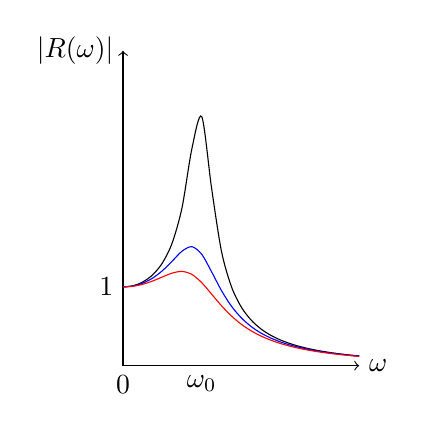
\begin{tikzpicture}
      \draw[->] (0,0) -- (3,0) node[right] {$\omega$};
      \draw[->] (0,0) -- (0,4) node[left] {$|R(\omega)|$};
      \draw[domain=0:3,smooth,variable=\x,black] plot ({\x},{1/sqrt((1-\x^2)^2+0.1*\x^2)});
      \draw[domain=0:3,smooth,variable=\x,blue] plot ({\x},{1/sqrt((1-\x^2)^2+0.5*\x^2)});
      \draw[domain=0:3,smooth,variable=\x,red] plot ({\x},{1/sqrt((1-\x^2)^2+0.9*\x^2)});
      \draw (0,0) node[below]{0};
\draw (0,1) node[left]{1};
\draw (1,0) node[below]{$\omega_0$};
\end{tikzpicture}
\end{center}
\item For $k<\frac{b^2}{2m}$, since $\omega_{res}$ has no real solution, then $|R(\omega)|$ monotonically decreases from 1 down to zero as $\omega$ increases.
\end{enumerate}
\end{ans}
\newpage
\begin{qns}[Waveguide]\leavevmode
\begin{enumerate}[label=(\roman*)]
\item Explain what is meant by dispersive waves, and distinguish between the group velocity and phase velocity of such waves.\hfill\textbf{[4]}
\item Give two examples of a dispersive wave.\hfill\textbf{[2]}\\[5pt]
A thin membrane has the property that transverse elastic waves travel in it at a speed $v$ that is independent of frequency and direction. A two-dimensional waveguide is made from this material. It is infinite in the $x$-direction, has width $b$ in the $y$-direction, and is rigidly fixed along the lines $y = 0$ and $y = b$ as shown in the diagram below.
\begin{figure}[H]
    \centering
    \includegraphics[scale=0.65]{2010P1B7Q.PNG}
\end{figure}
\item  Consider transverse elastic waves in this waveguide with wave vector $k = (k_x, k_y)$ and angular frequency $\omega$. What are the permitted values of $k_y$ and what is the general expression relating $\omega$ and $k_x$?\hfill\textbf{[4]}
\item Derive expressions for the phase and group velocities of guided waves travelling along the waveguide.\hfill\textbf{[3]}
\item If $b = 5$ cm and $\nu = 1000$ m s$^{−1}$, evaluate $k_x$ for travelling waves of frequency 15 kHz.\hfill\textbf{[3]}
\item Describe what would happen if you attempted to propagate waves of frequency (a) 5 kHz (b) 25 kHz.\hfill\textbf{[4]}
\end{enumerate}
\end{qns}
\begin{ans}\leavevmode
\begin{enumerate}[label=(\roman*)]
\item Dispersive waves change their profile as they propagate through a medium. If we consider a wave to be composed of many harmonic waves of different angular frequencies $\omega$ and wavenumbers $\mathbf{k}$, then the phase speed will be $v_p=\frac{\omega}{k}$ and in general, be dependent on $\omega$. The interference maximum will propagate at a group velocity given by $u_g=\frac{\partial\omega}{\partial k}|_{k_0}$ where $k_0$ is the dominant wavenumber in the group.
\item Water waves in the ocean, electromagnetic waves in a dielectric.
\item $\psi(x,0,t)=\psi(x,b,t)\implies k_yb=n\pi$ for $n\in\mathbb{Z}^+$. $$\omega=v\sqrt{k_x^2+k_y^2}=v\sqrt{k_x^2+(n\pi/b)^2}$$
\item $$u_p=\frac{\omega}{k_x}=v\sqrt{1+(n\pi/bk_x)^2},\quad u_g=\frac{\partial\omega}{\partial k_x}=\frac{vk_x}{\sqrt{k_x^2+(n\pi/b)^2}}$$ then $u_pu_g=v^2$.
\item 
$$k_x=\sqrt{(2\pi f/v)^2-(n\pi/b)^2}=\pi\sqrt{900-400 n^2},\quad k\in\mathbb{Z}^+$$ 
For $n=1$, $k_x=10\sqrt{5}\pi\in\mathbb{R}$. (b) If $f=25\times10^3$ Hz, then $k_x\in\mathbb{R}$ for both $n=1$ and $n=2$. (a) If $f=5\times10^3$ Hz, then $k_x\notin\mathbb{R}$, i.e. no propagating modes can be activated. 
\end{enumerate}
\end{ans}
\newpage
\begin{qns}[Fraunhofer Diffraction]\leavevmode
\begin{enumerate}[label=(\roman*)]
\item A 1-dimensional aperture is illuminated by a parallel beam of light of wavelength $\lambda$ and the diffraction pattern is viewed on a distant screen. Show that the amplitude of the diffraction pattern is given by
$$\psi(\theta)\propto\int_{-\infty}^\infty T(y)\exp\bigg(\frac{i2\pi y\sin\theta}{\lambda}\bigg)dy$$
where $\theta$ is the angular coordinate of a point on the screen as seen from the aperture and $T(y)$ is the transmission function of the aperture at distance $y$ from the centre of the aperture.\hfill\textbf{[4]}\\[5pt]
A pair of narrow slits separated by 0.1 mm is illuminated by light at a wavelength of 500 nm. Over one slit is placed a piece of glass which shifts the phase of the light going through that slit by 180\degree compared with the light going through the other slit.
\item Sketch
\begin{enumerate}[label=(\alph*)]
    \item the transmission function $T(y)$ for this aperture;\hfill\textbf{[2]}
    \item the intensity profile of the diffraction pattern as a function of angular coordinate on the diffraction screen.\hfill\textbf{[4]}
\end{enumerate}
\item The pair of narrow slits is replaced by an aperture consisting of a single slit 0.2 mm wide. Sketch the intensity of the diffraction pattern of this slit.\hfill\textbf{[3]}
\item Half of this slit is now covered by a piece of the same glass sheet described previously. Show how the diffraction pattern for this slit can be related to the diffraction pattern of the pair of slits and the diffraction pattern of a single slit of finite width. Sketch the intensity profile of the resulting diffraction pattern.\hfill\textbf{[7]}
\end{enumerate}
\end{qns}
\begin{ans}\leavevmode
\begin{enumerate}[label=(\roman*)]
\item Focusing on the linear phase variation (as seen from any given point on the aperture plane), the Fresnel-Kirchoff diffraction integral can be approximated as
$$\psi(\theta)\propto\int_\Sigma\psi_\Sigma e^{-ikyy_0/R}dy$$
where $\psi_\Sigma$ is the incident amplitude on the aperture plane $\Sigma$, $k=\frac{2\pi}{\lambda}$ is the wavelength of light used, $r$ is the distance from a point on the aperture plane $(x_0,y_0)$ to the point on screen $(x,y)$.
$$r=\sqrt{(y-y_0)^2+L^2}\approx R\bigg(1-\frac{2yy_0}{2R^2}\bigg)$$
where $R^2=y_0^2+L^2$, $R>>y,y_0$, and the higher order terms have been dropped. Assume small angle approximation, $\sin\theta\approx\tan\theta=\frac{y_0}{R}$, then
$$\int_\Sigma\psi_\Sigma e^{-iky_0y/R}dy\sim\int_{-\infty}^\infty T(y)e^{-iky_0y/R}dy\approx\int_{-\infty}^\infty T(y)e^{-i2\pi y\sin\theta/\lambda}dy$$
\item 
\begin{enumerate}[label=(\alph*)]
\item Let the separation of the two narrow slits be $2L=0.1$ mm. Sketch $T(y)=(\delta(y+L)-\delta(y-L))\otimes\text{rect}(y/\epsilon)$ where $\epsilon$ is very small since the slits are very narrow.
\begin{center}
\begin{tikzpicture}
\begin{axis}[
ticks=none,
width=10cm,
height=4cm,
x axis line style={-stealth},
y axis line style={-stealth},
xticklabels={},
ymax = 1.5,xmax=2.5,
axis lines*=center,
xlabel near ticks,
ylabel near ticks]
\addplot+[thick,mark=none,const plot]
coordinates
{(-2,0)(-2,-1)(-1,-1)(-1,0)(0,0)(1,0) (1,1) (2,0)};
\end{axis}
\end{tikzpicture}
\end{center}
\item The Fourier transform is $\propto e^{-iqL}-e^{iqL}=2\sin(qL)$, where $q=k\sin\theta=4\times 10^6\pi\sin\theta$. For very small $\theta$ (period is very small anyways), $I\propto\sin^2(200\pi\theta)$.
\begin{center}
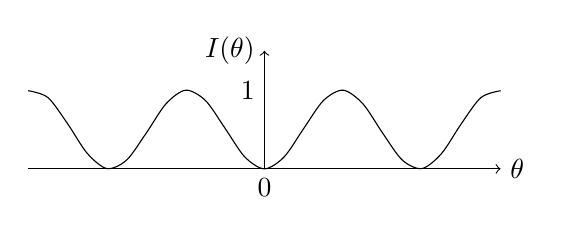
\begin{tikzpicture}
      \draw[->] (-3,0) -- (3,0) node[right] {$\theta$};
      \draw[->] (0,0) -- (0,1.5) node[left] {$I(\theta)$};
      \draw[domain=-3:3,smooth,variable=\x,black] plot ({\x},{(sin(200*pi*\x))^2});
      \draw (0,0) node[below]{0};
\draw (0,1) node[left]{1};
\end{tikzpicture}
\end{center}
\end{enumerate}
\item Let the width of the new slit be $l=0.2$ mm. The transmission function is now $T(y)=\text{rect}(y/l)$, then the Fourier transform is $\int_{-l/2}^{l/2}e^{-iqy}dy=l\sinc(lq/2)$
$$\implies I\propto\sinc^2(400\pi\sin\theta)\approx\sinc^2(400\pi\theta)$$
\begin{center}
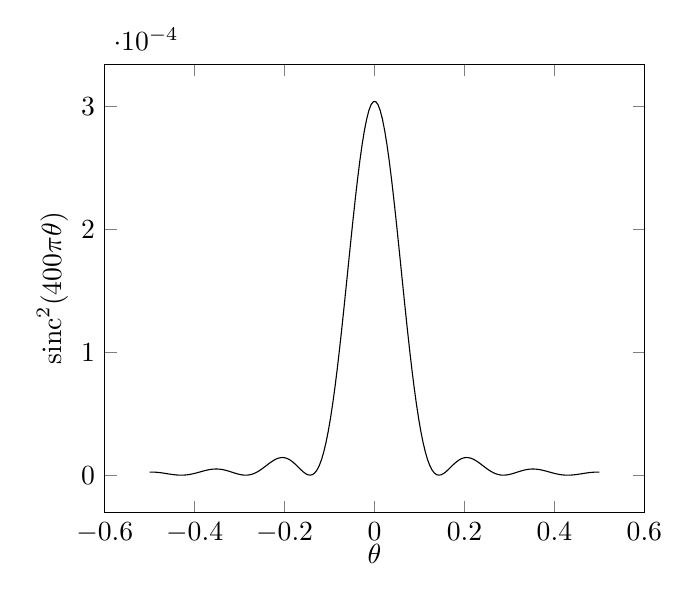
\begin{tikzpicture} 
    \begin{axis}[
    x label style={at={(axis description cs:0.5,-0.05)},anchor=north},
    y label style={at={(axis description cs:-0.05,.5)},anchor=south},
    ylabel={$\sinc^2(400\pi\theta)$},
    xlabel={$\theta$}]
      \addplot [domain = -0.5:0.5, samples = 200]
      ({\x},{(sin(400*pi*\x)/(400*pi*\x))^2});
 \end{axis}
\end{tikzpicture}
\end{center}
\item $T(y)$ is now $1$ for $0<y<l$ and $-1$ for $-l<y<0$. The Fourier transform will thus be $\propto\int_0^{l}e^{-ik\sin\theta y}dy-\int_{-l}^0e^{-ik\sin\theta y}dy=\frac{4}{iq}\sin^2(2qd)$. The intensity is hence 
$$I\propto\frac{\sin^4(400\pi\sin\theta)}{\sin^2\theta}\approx\sin^4(400\pi\theta)/\theta^2$$
In fact, this satisfies Convolution Theorem. The result for (iib) and (iii) are $2\sin(qL)$ and $l\sinc(lq/2)$ respectively. Multiplying together gives $$2l\sin(qL)\sinc(lq/2)=8d\sin(2qd)\sinc(2qd)=\frac{4}{q}\sin^2(2qd)$$
\begin{center}
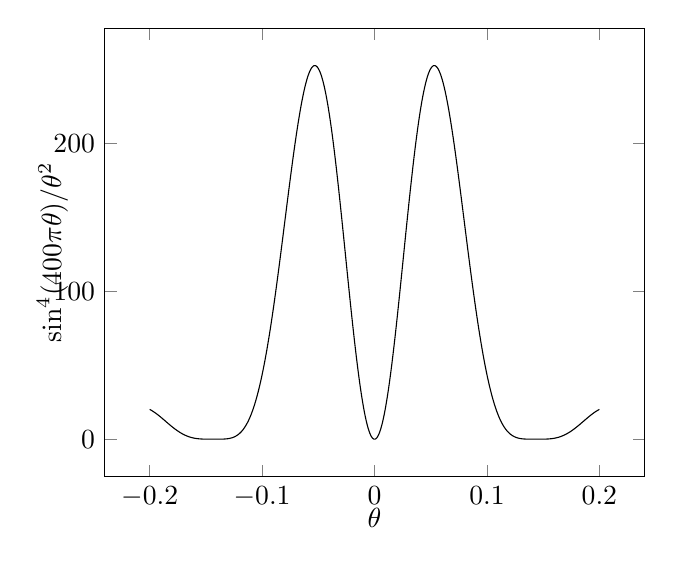
\begin{tikzpicture} 
    \begin{axis}[x label style={at={(axis description cs:0.5,-0.05)},anchor=north},
    y label style={at={(axis description cs:-0.05,.5)},anchor=south},
    ylabel={$\sin^4(400\pi\theta)/\theta^2$},
    xlabel={$\theta$}]
      \addplot [domain = -0.2:0.200, samples = 2000] ({\x},{(sin(400*pi*\x))^4/\x^2});
 \end{axis}
\end{tikzpicture}
\end{center}
\end{enumerate}
\end{ans}
\newpage
\begin{qns}[Fresnel Diffraction]\leavevmode
\begin{enumerate}[label=(\roman*)]
\item State the difference between Fresnel and Fraunhofer diffraction.\hfill\textbf{[2]}
\item Show that when a diffracting aperture is illuminated by a parallel beam of light, the transition between the Fresnel and Fraunhofer diffraction regimes occurs at a distance of approximately $\rho^2/\lambda$ from the aperture, where $\rho$ is a characteristic dimension of the aperture and $\lambda$ is the wavelength.\hfill\textbf{[3]}
\item A small radio receiver operating at a frequency of 30 GHz is 16 m away from a straight, very tall sheet metal fence. One day, a section of the fence is blown away in a storm, leaving a 0.5-metre-wide gap in the fence close to its point of closest approach to the radio receiver. Derive whether Fresnel or Fraunhofer diffraction should be used to calculate the amount of power detected by the receiver, due to the radiation leaking through the gap from a distant transmitter close to the ground.\hfill\textbf{[2]}\\[5pt]
The graph below is the Cornu spiral which gives the values of the integrals $C(w) =\int_0^w\cos(\pi y^2/2) dy$ and $S (w) =\int_0^w\sin(\pi y^2/2) dy$. The dimensionless coordinate $w$ corresponds to a distance $x$ from the optical axis given by $x\sqrt{2/\lambda z}$ where $z$ is the distance between the diffracting aperture and the point at which the diffraction is measured.
\begin{figure}[H]
    \centering
    \includegraphics[scale=0.75]{2010P1B9Q.PNG}
\end{figure}
\item The line-of-sight between the transmitter and the receiver grazes one edge of the gap in the fence. Draw a sketch of the Cornu spiral superimposed with suitable vectors corresponding to (a) the signal received through the gap and (b) the signal that would be received if the entire fence had blown down.\hfill\textbf{[5]}
\item What is the ratio of the power received in cases (a) and (b)?\hfill\textbf{[4]}
\item Which contiguous region of fence would have to be removed to receive the maximum signal from the transmitter?\hfill\textbf{[4]}
\end{enumerate}
\end{qns}
\newpage
\begin{ans}\leavevmode
\begin{enumerate}[label=(\roman*)]
\item The Fraunhofer regime occurs when the variation in phase along the observation screen is approximately linear in the distance in the aperture plane. The quadratic and higher order variations can only be neglected if their extra path difference from one extreme of the aperture to another is very much less than half a wavelength. The Frensel regime occurs when the quadratic terms cannot be neglected, but the cubic and higher terms can.
\item Consider a spherical source with strength $a_S$, at distance $s(x,y)$ from the aperture element $dxdy$ with overall aperture function $h(x,y)$. The incoming spherical wave have amplitude $\psi_1=a_Se^{iks}/s$, and the aperture element acts as a source of secondary wavelets with amplitude $-(i/\lambda)\psi_1(x,y)h(x,y)dxdy$. This secondary wave generates a disturbance at point P and have amplitude $d\psi_P$. Integrating everywhere gives us the total amplitude at point P, at a distance $r(x,y)$ from the aperture element
$$\psi_P=-\int\frac{i}{\lambda}h(x,y)K(\theta)\frac{a_Se^{ik(s+r)}}{sr}dxdy$$
where $K(\theta)$ is the obliquity factor to ensure momentum of photons is conserved. Consider the diffraction pattern in a plane at a distance $L$ from the aperture. We denote the coordinates of point P in this plane by $(x_0,y_0)$ and further assume P to be close to the axis. Assume that the source S is a large distance behind the aperture, and the aperture is illuminated with a plane wave at normal incidence.\\[5pt]
Considering P close to the axis such that $K=1$ and $x_0/L<<1$, $y_0/L<<1$, then the distance $r$ from the aperture element $dxdy$ to P is
$$r^2=L^2+(x_0-x)^2+(y_0-y)^2=D^2\bigg(1-2\frac{x_0x+y_0y}{D^2}+\frac{x^2+y^2}{D^2}\bigg)$$
where $D^2=L^2+x_0^2+y_0^2$. Using binomial expansion, we obtain $r\approx D-\frac{x_0x+y_0y}{D}+\frac{x^2+y^2}{2D}$. Since the phase of each wavelet is directly proportional to $kr$, the phase will have terms which vary linearly and quadratically with the position in the aperture. For large $D$, we obtain the Fraunhofer diffraction condition $\forall x,y\in\Sigma$, where we can drop the quadratic term and left with the linear term. Equivalently, for an aperture of maximum extent $\rho=\sqrt{x^2+y^2}$, the quadratic term for the phase $kr$ must be much less than $\pi$, i.e. $\frac{x^2+y^2}{2D}k<<\pi\implies D>>\frac{\rho^2}{\lambda}$.
\item We compute $\frac{\rho^2}{\lambda}=\frac{(0.5)^2(30\times10^9)}{3\times10^8}=25$ m. This is of the same order of magnitude as 16 m, so this is the Frensel regime.
\item The vectors for (b) and (a) respeectively are from $(0.5,0.5)$ to $(-0.5,-0.5)$ and from $(0.5,0.5)$ to $(0,0)$.
\item Since the ratio of amplitudes is half, the ratio of power is a quarter, with (b) being larger.
\item Maximum amplitude occurs for the interval $\Delta w=2.4$. This is the longest spanning vector between any two points on the Cornu spiral. Further, to convert between $x$ and $w$:
$$w=x\sqrt{\frac{2}{\lambda z}}=x\sqrt{\frac{(2)(30\times10^{-9})}{(3\times10^8)(16)}}=3.5355 x$$
Hence, $x=0.6788$ m. Since the transmitter is distant, we approximate the opening as $x$. Since the current opening is already 0.5 m, we need to remover another 0.1788 m above the current fence height.
\end{enumerate}
\end{ans}
\newpage
\subsubsection{Section C}
\begin{qns}[Brillouin Zone]\leavevmode
\begin{enumerate}[label=(\roman*)]
\item Sketch the typical energy–wavevector dependence, or dispersion relation, of electrons in a one-dimensional periodic potential within nearly free electron theory. In your sketch, include the unperturbed dispersion, the effects of the periodic potential, the Brillouin zone, the relevant reciprocal lattice wavevector, and the folded-back band structure. How can this approach explain the formation of energy gaps in solids?\hfill\textbf{[6]}
\item In the first Brillouin zone of a body centred cubic (BCC) crystal, the shortest distance from the zone centre to the zone boundary is $\sqrt{2}\pi/a$, where $a$ is the width of the conventional cubic unit cell. Show that in free electron theory the Fermi wavevector $k_F$ is $(3\pi^2n)^{1/3}$, where $n$ the number density of electrons, and demonstrate that the free electron Fermi surface of a monovalent metal with the BCC structure is contained entirely within the first Brillouin zone.\hfill\textbf{[5]}
\item The absorption of photons in metals excites an electron from a filled state at wavevector $k$ to an empty state at the same wavevector, but in a higher band. Sketch a suitable one-dimensional electronic dispersion relation and indicate the absorption process that requires the minimum energy $E_0$. For a BCC monovalent material, show that this energy is approximately 0.64 times the Fermi energy $E_F$.\hfill\textbf{[5]}\\[5pt]
Alkali metals have a BCC structure. The experimental data below show the frequency dependence of the conductivity in the alkali metals Na, K, and Rb, which have lattice constants $a$, respectively, of 0.423 nm, 0.523 nm, and 0.559 nm.
\begin{figure}[H]
    \centering
    \includegraphics[scale=0.65]{2010P1C10Q.PNG}
\end{figure}
\item The broad peaks at higher frequencies in each curve have been interpreted as arising from interband optical absorption. Explain whether this is qualitatively consistent with nearly free electron behaviour.\hfill\textbf{[4]}
\end{enumerate}
\end{qns}
\newpage
\begin{ans}\leavevmode
\begin{enumerate}[label=(\roman*)]
\item

\item 



\item

\item

\end{enumerate}
\end{ans}
\newpage
\begin{qns}[Band Structure]\leavevmode
\begin{enumerate}[label=(\roman*)]
\item Show that the mobility (ratio of drift velocity to electric field) of electrons in solids is $\mu=e\tau/m_e^*$ , where $\tau$ is relaxation time and $m_e^*$ is the effective mass. Hence show that the resulting electrical conductivity is given by $\sigma=ne^2\tau/m_e^*$, where $n$ is the conduction electron number density.\hfill\textbf{[5]}
\item A semiconductor has a band gap energy $E_g = 1$ eV and equal electron and hole effective masses, $m_e^*=m_h^*$. Show that at 300 K, intrinsic conduction in this material is negligible compared to that of a typical metal.\hfill\textbf{[4]}
\item The semiconductor is n-doped with a donor concentration of $N_d = 10^{18}$ cm$^{−3}$. On an energy band diagram, indicate the position of the conduction and valence bands, the chemical potential of the undoped semiconductor, the position of the donor levels and the chemical potential of the doped semiconductor. Calculate the electrical conductivity of the doped semiconductor at 300 K, given an electron mobility of $\mu= 100$ cm$^2$ V$^{−1}$s$^{−1}$, and assuming that the donors are fully ionised.\hfill\textbf{[6]}
\item The semiconductor has a dielectric constant $\epsilon=18$ and an effective mass for electrons $m_e^* = 0.015m_e$. Calculate the ionisation energy and estimate the extent of a hydrogenic donor orbit, and comment on whether the assumption of full ionisation of the donors is justified.\hfill\textbf{[5]}

\begin{mdframed}
\color{darkblue}{The ionisation energy of Hydrogen is 13.6 eV, and the Bohr radius is $5.3\times 10^{−11}$ m.}
\end{mdframed}
\end{enumerate}
\end{qns}
\begin{ans}\leavevmode
\begin{enumerate}[label=(\roman*)]
\item In dynamic equilibrium, the net force on the electrons averages to zero, hence
$$\boldsymbol{0}=m_e^*\mathbf{\ddot{r}}=-e\mathbf{E}-\gamma\mathbf{\dot{r}}$$
Assuming a linear friction term $\gamma$, we have $|\mathbf{\dot{r}}|/|\mathbf{E}|=e/\gamma$. If we solve the equation of motion without the electric field, we have 
$$m_e^*\mathbf{\ddot{r}}+\gamma\mathbf{\dot{r}}=\boldsymbol{0}\implies\mathbf{r}=\mathbf{A}+\mathbf{B}e^{-\gamma t/m_e^*}$$
Thus the characteristic decay time $\tau$ is given by $\tau=m_e^*/\gamma$ and hence we obtain the mobility $\mu=e\tau/m_e^*$. The electrical conductivity in isotropic linear materials is $\sigma$ and satisfies $\mathbf{J}=\sigma\mathbf{E}$, where $\mathbf{J}$ is the current density per unit area, and is related to the number density of electrons by
$$\mathbf{J}=ne\mathbf{\dot{r}}\implies\sigma=\frac{|\mathbf{J}|}{|\mathbf{E}|}=\frac{ne\mu|\mathbf{E}|}{|\mathbf{E}|}=\frac{ne^2\tau}{m_e^*}$$
\item To compare the relative conductances, we need to know the relative populations of charge carriers and the relative effective masses. For an undoped semiconductor, the chemical potential lies halfway within the bandgap, and hence the populations are suppressed by a factor of $e^{-E_g/2k_BT}$, assuming similar effective masses
$$\frac{\sigma_{semicon}}{\sigma_{metal}}\sim e^{-E_g/2k_BT}\sim e^{-1.6\times10^{-19}/(2(1.38\times10^{-23})(300))}\sim 10^{-9}$$
\item For an undoped semiconductors for electrons of wavenumbers $\mathbf{k}$ and energy $E(\mathbf{k})$, we have parabolic conduction and valence bands with turning points facing each other. The chemical potential $\mu$ is midway between this energy gap $E_g$. The introduction of $n$-type dopants create localized states in real space and hence delocalized states in $k$-space energy levels. These levels are very slightly below the empty conduction band, and have the effect of dragging $\mu$ towards the top of the bandgap. The electrical conductivity of the fully ionized donors is
$$\sigma=N_de\mu=10^{18}(1.6\times10^{-19})(100)(100)=1.6\times10^3\Omega^{-1}m^{-1}$$
\item The energy levels of a Hydrogen atom are of the form $E_n=-R_H/n^2$, where $R_H=13.6$ eV is the Rydberg constant, which depends on the mass of the electron $m$ and relative dielectric constant $\epsilon$ via $R_H\propto m/\epsilon^2$, and so for the dopants, the ionization energy is
$$E_{ionization}=13.6\times\frac{0.05}{18^2}=6.296\times10^{-4}eV$$
This is very much smaller than the bandgap, and hence justifies placing the donor Hydrogenic orbits so close to the conduction band. At 300 K, all the donors will be excited as $E_{ionization}<<k_BT$. For Hydrogen atoms, the Bohr radius $a_0$ represents the modal radius of the probability distribution for the ground state
$$a_0=\frac{4\pi\epsilon_0\hbar^2}{e^2m_e}$$
and so for the dopant atoms, the modal radius $a'$ is
$$a'=a_0\frac{18}{0.015}=\frac{18}{0.015}\frac{4\pi(8.85\times10^{-12})(6.626\times10^{-34}/2\pi)^2}{(1.6\times10^{-19})^2(9.11\times10^{-31})}=63.6nm$$
A dopant concentration of $N_D$ roughly corresponds to a dopant-dopant separation $l=N_D^{-1/3}=10$ nm $<a'$, so donors are not isolated orbitals.
\end{enumerate}
\end{ans}
\subsubsection{Section D}
\begin{qns}[OWO Short Note]
Write brief notes on two of the following:\hfill\textbf{[20]}
\begin{itemize}
    \item resolving a pair of narrow spectral lines using two different optical instruments;
    \item the transient response of a damped oscillator;
    \item the propagation of sound waves in gases. 
\end{itemize}
\end{qns}
\begin{ans}\leavevmode
\subsubsection*{Resolving a pair of narrow spectral lines using two different optical instruments:}
The two optical instruments we will discuss are the Fabry-Pérot etalon and the Michelson interferometer. For Michelson-Morley interferometer, the path difference is generated by only one reflection not many (like in the Fabry-Pérot etalon), and hence its physical dimensions need to be larger by a factor of the order $m$, in order to achieve the same resolution.\\[5pt]
Consider a film of air (of thickness $d$) sandwiched between two mirrors, known as a Fabry-Pérot etalon. A fraction $t$ of this beam is transmitted in passing from glass to air, and a further fraction $t'$ transmitted in passing from air to glass, giving an emerging beam of amplitude $tt'=T$. This etalon produces a fringe pattern with much sharper features than a simple thin film, and is useful for high resolution spectroscopy. \\[5pt]
Each successive beam emerging from the etalon acquires a factor of $R:=r^2$ in amplitude and a phase shift $\delta$, where $\delta=\frac{4\pi d}{\lambda}\cos\theta$ (thin film). The total intensity transmission of the etalon is $|A|^2$ where $A=Te^{i\omega t}\sum_{n=0}^\infty R^ne^{-in\delta}$:
$$\frac{Te^{i\omega t}}{1-Re^{-i\delta}}\frac{Te^{-i\omega t}}{1-Re^{i\delta}}=\bigg|\frac{T}{1-Re^{i\delta}}\bigg|^2=\frac{T^2}{(1-R\cos\delta)^2+R^2\sin^2\delta}=\frac{T^2}{(1-R)^2}\bigg(\frac{1}{1+(4R/(1-R)^2))\sin^2(\delta/2)}\bigg)$$
The fringe pattern has maxima at $\delta=\frac{4\pi d}{\lambda}\cos\theta=2m\pi$ for $m\in\mathbb{Z}^+$. At normal incidence $\theta=0$ we have an integer number of half wavelengths between the mirrors.\\[5pt]
Although a Fabry-Pérot etalon will in general produce narrow and sharply defined circular fringes (of constant inclination $\theta$), in practice use them at normal incidence and detect the transmitted intensity at angles very close to $\theta=0$. By varying the spacing of the mirrors and using a photodiode to measure the transmitted intensity it is possible to measure the spectrum of the incident light, with each wavelength component producing its own set of peaks as a function of $d$.\\[5pt]
In practice, one cannot sum the geometric series to infinity above as it assumes that the etalon is infinite in extent (and that the plates are perfectly parallel, with uniform reflectivites), and so we have a finite total path difference, which will blur this resolution.
\begin{figure}[H]
    \centering
    \includegraphics[width=\linewidth]{fabryperot.PNG}
    \caption{(Top Left) Geometry of Fabry Pérot Etalon. (Top Right) Free Spectral Range and Resolution of Fabry Pérot Etalon. (Bottom Left) Intensity Profile of Fabry Pérot Etalon. (Bottom Right) Finesse Profile of Fabry Pérot Etalon.}
\end{figure}
The sharpness of the peaks is a function of $\delta$. The maximum value of $\frac{I_{out}}{I_{in}}=\frac{T^2}{(1-R)^2}$ where $\delta=2m\pi$. We define the half-width of the peaks $\delta_{1/2}$ as the change in $\delta$ required for the intensity to reduce to half its maximum value.
$$\frac{4R}{(1-R)^2}\sin^2(0.5\delta_{1/2})=1\implies\delta_{1/2}\approx\frac{1-R}{\sqrt{R}}$$
It is useful to define the finesse, $\mathcal{F}$ as the ratio of separation of successive peaks in $\delta$ (equal to $2\pi$) to their full-width at half maximum $(2\delta_{1/2})$
$$\mathcal{F}=\frac{2\pi}{2\delta_{1/2}}=\frac{\pi\sqrt{R}}{1-R}$$
The finesse is a measure of the quality of the etalon and becomes high as $R\rightarrow 1$. The chromatic resolving power of the etalon is defined as $\frac{\lambda}{\Delta\lambda}$.
$$d\delta=-\frac{4\pi d\cos\theta}{\lambda^2}d\lambda\implies|d\delta|:=\Delta\delta=\frac{\delta}{\lambda}\Delta\lambda=2\delta_{1/2}\implies\frac{\lambda}{\Delta\lambda}=\frac{2\pi d\cos\theta}{\lambda\delta_{1/2}}$$
Since $2d\cos\theta=m\lambda$ at maxima, the resolving power is $\frac{\lambda}{\Delta\lambda}=\frac{m\pi}{\delta_{1/2}}=m\mathcal{F}$. This has the same form as the resolving power in the $m$th order for a diffraction grating of $N$ lines, where $N_{eff}$ is $\mathcal{F}$ of the Fabry-Pérot interferometer. This effective number is also the number of interfering beams in the interferometer.\\[5pt]
If $R=0.95$, $d=5$ mm, $\lambda=500$ nm, the resolving power is more than $10^6$ comparable with a grating spectrometer with a very large grating. Unfortunately, neighbouring orders with different wavelengths will overlap. The wavelength difference at which this  overlapping takes place is known as the free spectral range. At normal incidence, the maxima is at $2d=m\lambda\implies-\frac{2d}{\lambda^2}d\lambda=dm$. When $m$ is large, we can use this to find the wavelength change $(\Delta\lambda)_{fsr}$ corresponding to $\Delta m=1$, i.e.
$$1=\Delta m\frac{2d}{\lambda^2}(\Delta\lambda)_{fsr}=\frac{m}{\lambda}(\Delta\lambda)_{fsr}$$
The free spectral range $(\Delta\lambda)_{fsr}=\frac{\lambda}{m}$. The free spectral range around $\lambda=500$ nm is only 0.025 nm. Etalons are more suitable for measuring the fine structure of narrow spectral lines. The number of resolution elements across the spectrum is $\frac{(\Delta\lambda)_{fsr}}{(\Delta\lambda)_{res}}=\mathcal{F}$.\\[5pt]
The Michelson interferometer has many important applications including high precision metrology, Fourier Transform spectroscopy and the Michelson-Morley experiment. Consider the basic setup
\begin{figure}[H]
    \centering
    \includegraphics[width=\linewidth]{mmi.PNG}
\end{figure}
The beam-splitter splits the incident beam with components travel along different paths, and recombine at the same beam-splitter. Constructive or destructive interference will occur depending on the difference between the two paths. Normally, one path is kept fixed (reference path) and the other path is varied by moving a mirror (on a precision stage) in order to see a fringe pattern as a function of the mirror position. This arrangement focuses the beams onto a photodiode. The system is illuminated with the collimated beam; the mirrors are aligned so that the path difference is constant across the beam\\[5pt]
If a light source has two closely-spaced wavelengths $k_0\pm\Delta k$, each component will produce a fringe pattern with a slightly different fringe spacing. The observed interference pattern will be the sum of the two individual patterns. As $x$ increases from $x=0$, a phase shift develops between the two patterns and eventually the fringes become invisible since the maxima in one set of fringes overlap with the minima in the other set. The larger the spacing between the components $\Delta k$, the more rapidly fringes disappear as $x$ increases.\\[5pt]
Let the intensity of light in the wavenumber range $[k,k+dk]$ be $S(k)dk$ such that $S(-k)=S^*(k)$. In this double-sided convention for a spectrum, $S(k)$ can be represented as two pairs of closely-spaced delta functions spaced about $\pm k_0$. This can be written as a convolution $S(k)=[\delta(k-k_0)+\delta(k+k_0)]*[\delta(k-\Delta k)+\delta(k+\Delta k)]\implies I(x)=I_1[1+\cos(k_0x)\cos(\Delta kx)]$. The high frequency cosine $\cos(k_0x)$ represents the fringes while the low frequency envelope $\cos(\Delta kx)$ modulates the amplitude of these fringes. We can define the fringe contrast or fringe visibility as the ratio of local high-frequency fringe amplitude to the mean intensity.
$$\frac{I_{max}-I_{min}}{I_{max}+I_{min}}$$
At the position of the first zero in the low frequency envelope, the fringe contrast will be zero and this can be used to find $\Delta k$.\\[5pt]
Measuring the fringe visibility allows the fine structure of atomic lines to be investigated. The Sodium D line at 589.3 nm is in fact a doublet with $\Delta\lambda=0.6$ nm, whereas the Cadmium line is highly monochromatic, hence showing no minimum in fringe visibility for values of $x\leq 0.4$ m.
\newpage
\subsubsection*{The transient response of a damped oscillator:}
Consider the presence of a sinusoidal driving force in a damped oscillatory system such that the equation of motion has the form
$$\ddot{x}+\gamma\dot{x}+\omega_0^2x=f_0e^{i\omega t}$$
The driving frequency, $\omega$, is not necessarily equal to the natural frequency of oscillation, $\omega_0$. The general solution for a forced damped oscillatory system is a linear combination of the general solution for an unforced damped oscillatory system (associated homogeneous differential equation) and the particular solution for the forced function. The transient solution, complementary solution of the forced damped oscillation, is just the general solution of the corresponding homogeneous second order differential equation, i.e. free (but could be damped) oscillation.\\[5pt]
The homogeneous solutions for a damped oscillating system
$$\ddot{x}+\gamma\dot{x}+\omega_0^2x=0$$
are as follows:
\begin{enumerate}
    \item $x(t)=e^{-0.5\gamma t}[C_1e^{i\omega_ut}+C_2e^{-i\omega_ut}]$, where $\omega_u=\omega_0\sqrt{1-0.25(\gamma/\omega_0)^2}<\omega_0$.
    \item $x(t)=C_3e^{-\mu_1t}+C_4e^{-\mu_2t}$ where $\mu_{1,2}=0.5\gamma\pm\sqrt{-\omega_0^2+0.25\gamma^2}$.
    \item $x(t)=(C_5+C_6t)e^{-0.5\gamma t}$.
\end{enumerate}
where $C_1$, $C_2$, $C_3$, $C_4$ and $C_5$ are arbitrary constants that are dependent on boundary conditions. This is illustrated below: red, black blue respectively.
\begin{center}
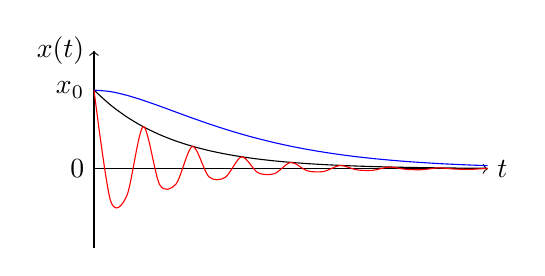
\begin{tikzpicture}
      \draw[->] (0,0) -- (5,0) node[right] {$t$};
      \draw[->] (0,-1) -- (0,1.5) node[left] {$x(t)$};
      \draw[domain=0:5,smooth,variable=\x,black] plot ({\x},{exp(-\x)});
      \draw[domain=0:5,smooth,variable=\x,blue] plot ({\x},{(1+\x)*exp(-\x)});
      \draw[domain=0:5,smooth,variable=\x,red] plot ({\x},{exp(-\x)*cos(10*\x*180/pi)});
      \draw (0,0) node[left]{0};
    \draw (0,1) node[left]{$x_0$};
\end{tikzpicture}
\end{center}
Suppose $\gamma<2\omega_0$, such that the damping is small, then the oscillation is said to be underdamped. The general solution for an underdamped solution is
$$x(t)=e^{-0.5\gamma t}(c_1\cos(\omega_ut)+c_2\sin(\omega_ut))$$
where $\omega_u=\sqrt{\omega_0^2-0.25\gamma^2}$ and the constants $c_1$ and $c_2$ are dependent on the initial conditions. If the initial conditions are $x(t=0)=x_0$ and $\dot{x}(t=0)=v_0$, then the solution is
$$x(t)=e^{-0.5\gamma t}\bigg(x_0\cos(\omega_ut)+\frac{v_0+0.5\gamma x_0}{\omega_u}\sin(\omega_ut)\bigg)$$
which is an oscillatory solution with a decaying envelope.\\[5pt]
If $\gamma>2\omega_0$, where there is a large friction, then the system is said to be overdamped such that no oscillation occurs and the displacement goes asymptotically to zero. The general solution is
$$x(t)=c_+e^{-\mu_+t}+c_-e^{-\mu_-t}$$
where $\mu_{\pm}=\frac{1}{2}\gamma\pm\sqrt{0.25\gamma^2-\omega_0^2}$ such that $\mu_+>0.5\gamma>\omega_0$ and that $c_{\pm}$ are constants dependent on initial conditions. With the initial conditions $x(t=0)=x_0$ and $\dot{x}(t=0)=v_0$, the constants are
$$c_+=\frac{x_0\mu_-+v_0}{\mu_--\mu_+},\quad c_-=\frac{x_0\mu_++v_0}{\mu_+-\mu_-}$$
For heavy damping, the greater the friction, the amplitude decreases at a slower rate and it takes a much longer time for the amplitude to reach zero.\\[5pt]
Critical damping occurs when $\gamma=2\omega_0$ and subjected to the initial conditions $x(0)=x_0$ and $v(0)=v_0$, we have
$$x(t)=(x_0+(v_0+0.5\gamma x_0)t)e^{-0.5\gamma t}$$
Critically damping gives the fastest return to the equilibrium position (but still asymptotically reaches zero), without undergoing oscillation.
\subsubsection*{The propagation of sound waves in gases:}
Recall the definition of longitudinal waves: The displacement of the medium in a longitudinal wave is in the same direction as the direction of wave propagation. Then, for a longitudinal wave in gas, we will show that the longitudinal displacement and excess pressure obey the wave equation.\\[5pt]
Let's consider a 1D wave, i.e. a tube of air inside a cylindrical container with cross-sectional area $A$. Let the ends of this section be located at $x$ and $x+\Delta x$ at equilibrium, and then at $x+\psi(x)$ and $x+\Delta x+\psi(x+\Delta x)$ at a later time. The function $\psi$ measures the longitudinal displacement from equilibrium. If we define $\Delta\psi$ to be $\psi(x+\Delta x)=\psi(x)+\Delta\psi$, where $\Delta\psi$ is how much more the right boundary of the region moves compared with the left boundary.\\[5pt]
Let the pressure in the tube at equilibrium be $p_0$. Let $\psi_p(x)$ be the excess pressure above $p_0$ as a function of $x$. The total pressure at the left boundary and the right boundary are $\psi_p(x)$ and $\psi_p(x+\Delta x)=\psi_p(x)+\Delta\psi_p$, where $\Delta\psi_p$ is how much the pressure at the right boundary exceeds the pressure at the left boundary.\\[5pt]
The change in volume from equilibrium $\Delta V=A\Delta\psi$ is directly proportional to $-V\psi_p$, where $\Delta V/V<<1$. Let the compressibility $\kappa$ be the desired constant of proportionality, then $$\frac{\partial\psi}{\partial x}=-\kappa\psi_p\implies\frac{\partial\psi_p}{\partial x}=-\frac{1}{\kappa}\frac{\partial^2\psi}{\partial x^2}$$
For ideal gas, we have isothermal compressibility be $\kappa=\frac{1}{p_0}$ and for adiabatic compressibility be $\kappa=\frac{1}{\gamma p_0}$. The net force is $F_{net}=A(p(x)-p(x+\Delta x))=A(p_0+\psi_p(x)-p_0-\psi_p(x+\Delta x))=A(-\Delta\psi_p)$ and so
$$\rho A\Delta x\frac{\partial^2\psi}{\partial t^2}=-A\bigg(-\frac{1}{\kappa}\frac{\partial^2\psi}{\partial x^2}\Delta x\bigg)\implies\frac{\partial^2\psi}{\partial t^2}=\frac{\gamma p_0}{\rho}\frac{\partial^2\psi}{\partial x^2}$$
The longitudinal displacement does satisfy the wave equation. Taking $\frac{\partial}{\partial x}$ yields $$\frac{\partial^2}{\partial t^2}\frac{\partial\psi}{\partial x}=\frac{\gamma p_0}{\rho}\frac{\partial^2}{\partial x^2}\frac{\partial\psi}{\partial x}$$
Since $\frac{\partial\psi}{\partial x}$ is directly proportional to $\psi_p$, we have the desired wave equation for excess pressure. The wave speed is $1/c=1/\sqrt{\rho/\gamma p_0}=1/\sqrt{\kappa\rho}$. The pressure leads the displacement by a phase $\pi/2$ and has amplitude $\frac{k}{\kappa}\psi$. For a harmonic wave of the form $\psi(x,t)\propto e^{i(\omega t-kx)}$, then $\psi_p(x,t)=-\frac{1}{\kappa}\frac{\partial\psi(x,t)}{\partial x}=-\frac{-ik}{\kappa}\psi(x,t)$. The excess force that a sheet of gas exerts on the region to its right is $$F=A\psi_p=A\bigg(-\frac{1}{\kappa}\frac{\partial\psi}{\partial x}\bigg)=-\frac{A}{\kappa}\bigg(\mp\frac{1}{c}\frac{\partial\psi}{\partial t}\bigg)=\frac{\pm A}{\kappa c}\frac{\partial\psi}{\partial t}$$
where we used the harmonic wave form. Hence, the acoustic impedance  $Z_{acous}$ (impedance per cross-sectional area) of the gas is $$Z_{acous}=\frac{1}{A}\frac{F}{\partial\psi/\partial t}=\frac{1}{\kappa c}=\sqrt{\rho/\kappa}=\sqrt{\gamma p_0\rho}$$
The energy density per unit volume can be shown to be $\rho(\frac{\partial\psi}{\partial t})^2$ where $A\rho=\mu$. The power on the sheet of particles whose equilibrium position is $x$ is $P=(p_0+\psi_p)A\frac{\partial\psi}{\partial t}$. Since $\psi_p=-\frac{1}{\kappa}\frac{\partial\psi}{\partial x}$, then $$P=\pm\frac{A}{\kappa c}\bigg(\frac{\partial\psi}{\partial t}\bigg)^2=\pm\frac{Ac^2\kappa^2}{\kappa c}\psi_p=\frac{c}{\rho c^2}\psi_p=\frac{\psi_p}{\rho c}$$ 
Alternatively, using the acoustic impedance $Z_{acous}=\rho c$, we have $P=\pm Z_{acous}(\frac{\partial\psi}{\partial t})^2$. The mean power per unit area, or intensity, is  $\frac{1}{2}Z_{acous}\omega^2|\psi_0|^2$. We can express the intensity of sound as a power level in decibels:
$$10\log_{10}(I/I_{ref})$$
with $I_{ref}=p_{ref}^2/Z_{acous}$ which is $10^{-12}$ W/m$^2$, where $Z_{acous}$ for air is 400 kg m$^{-2}$ s$^{-1}$.
\end{ans}
\newpage
\begin{qns}[CMP Essay]
Explain the ideas underlying our understanding of the thermal conductivity of solids. Your discussion should include (i) why it is appropriate to apply the theory of gases result $\kappa=\frac{1}{3}C\langle c\rangle\ell$ to solids, where $C$ is the heat capacity per unit volume, $\langle c\rangle$ is an average speed and $\ell$ is a mean free path, (ii) thermal transport by phonons and electrons, (iii) scattering mechanisms limiting the mean free path $\ell$, and (iv) the Wiedemann–Franz law.\hfill\textbf{[20]}
\end{qns}
\begin{ans}
In general, we account for the thermal conductivity of insulators and metals by phonons and electrons respectively. 
\subsubsection*{Theory of gases and thermal transport by phonons:}
We use the kinetic theory of gases to model phonons (which are predominant carriers of heat in insulators): we consider phonons crossing a plane at an angle $\theta$, the excess temperature of phonons crossing the plane $\Delta T=-\frac{dT}{dz}\ell\cos\theta$ and excess energy in each phonon mode $c_{ph}\Delta T=-c_{ph}\frac{dT}{dz}\ell\cos\theta$, where $c_{ph}$ is the heat capacity of a phonon mode. We integrate the excess heat per mode over the phonon distribution $nf(c)dc$, i.e. the number of phonons with speed $c$ to $c+dc$. The phonons are propagating in all directions, so weight by speed normal to the plane. The fraction with angles $\theta$ to $\theta+d\theta$ is $\frac{2\pi}{4\pi}\sin\theta d\theta$. The heat flux integral across the plane becomes
$$\int_0^\pi\int_0^\infty nf(c)dc\frac{1}{2}\sin\theta d\theta c\cos\theta\bigg(-c_{ph}\frac{dT}{dz}\ell\cos\theta\bigg)=-\frac{1}{2}c_{ph}n\ell\frac{dT}{dz}\int_0^\pi\sin\theta\cos^2\theta d\theta\langle c\rangle$$
Since this heat flux is $-\kappa\frac{dT}{dz}$, we obtain our desired result: $\kappa=\frac{1}{3}C\langle c\rangle \ell$ where $C$ is the heat capacity per unit volume, $\langle c\rangle$ is the average speed, and $\ell$ is the phonon mean free path. This result also holds for electrons in metals, as we will discuss later.
\subsubsection*{Thermal transport by electrons:}
In the free electron model (FEM), each lattice point contributes $n$ delocalized electrons ($n$ is valency). The rest are regarded as core electrons and together with the nuclei, they form a uniform background potential. With this in mind, we can predict the transport properties of these solids using the classical Drude model. The assumptions of the Drude model are
\begin{enumerate}
    \item Independent electron approximation: neglect electron-electron interactions between collisions; Free electron approximation: neglect electron-ion interactions. The electrons respond solely to the externally applied fields.
    \item Collisions are instantaneous events that abruptly alter the velocity of an electron. Drude attributed them to the electrons bouncing off the impenetrable ion cores.
    \item Electron experiences a collision with a probability per unit time $1/\tau$, where $\tau$ is the relaxation time. An electron picked at random at a given moment will, on the average, have been travelling for a time $\tau$ before its next collision, and will, on the average, have been travelling for a time $\tau$ since its last collision. $\tau$ is independent of the electron's position and velocity.
    \item Electrons are assumed to achieve thermal equilibrium with their surroundings only through collisions. Immediately after each collision, an electron is taken to emerge with a velocity that is not related to its velocity just before the collision, but randomly oriented and with a speed appropriate to the temperature prevailing at the place where the collision occurred.
\end{enumerate}
In the Drude's derivation, one uses classical statistical mechanics on a metallic electron gas. The Sommerfeld model uses quantum statistical mechanics instead. The Fermi-Dirac distribution is
$$n_{FD}=\frac{1}{e^{(\epsilon-\mu)/k_BT}+1}$$
Under Born-von Karman boundary conditions (or sometimes called periodic boundary conditions), the solution is $\psi_k(\mathbf{r})=\frac{1}{\sqrt{V}}e^{i\mathbf{k}\cdot\mathbf{r}}$ with energy $\epsilon(\mathbf{k})=\frac{\hbar^2k^2}{2m}$. The periodic boundary condition require quantization of wavevectors $k_i=\frac{2\pi n_i}{L}$, $n_i\in\mathbb{Z}$. If the region is very large, then to an excellent approximation, the number of allowed points is just the volume of $k$-space contained within the region, divided by the volume of $k$-space per point in the network of allowed values of $\mathbf{k}$. We conclude that a region of $k$-space of volume $\Omega$ will contain $\frac{\Omega V}{8\pi^3}$ allowed values of $\mathbf{k}$.\\[5pt]
Assuming the electrons are non-interacting, we can build up the $N$-electron ground state by placing electrons into the allowed one-electron levels. The Pauli exclusion principle states that we at most place on electron in each single electron level. But, associated with each allowed wavevector $\mathbf{k}$ are two electronic levels.\\[5pt]
We begin placing the electrons from the lowest energy and then successively filling the one-electron levels of lowest energy that are not occupied. Since the energy of a one-electron level is directly proportional to the square of its wave vector, when $N$ is enormous, the occupied region will be indistinguishable from a sphere. The radius of this sphere is called $k_F$ and its volume $\Omega$ is $\frac{4}{3}\pi k_F^3$. The corresponding highest energy occupied state is the Fermi energy $E_F$. The number of allowed values of $\mathbf{k}$ within the sphere is $\frac{4\pi k_F^3}{3}\frac{V}{8\pi^3}=\frac{k_F^3V}{6\pi^2}$. The number of electrons will be twice of this and so the electronic density is $n=\frac{k_F^3}{3\pi^2}$.\\[5pt]
When an electric field is applied, the electrons start to move. Since they have extra momentum, the electron states are displaced in $k$-space. In the absence of scattering, the equation of motion is $\frac{d\mathbf{k}}{dt}=-\frac{e\mathbf{E}}{\hbar}$. In reality, electrons do not accelerate indefinitely since scattering processes occur to limit the displacement of the Fermi sphere. The electronic contribution to thermal conductivity is
$$\kappa_{el}=\frac{1}{3}C_{el}\langle c\rangle\ell=\frac{1}{3}\frac{\pi^2nk_BT}{2T_F}v_F\tau=\frac{\pi^2nk_B^2T\tau}{3m^*}$$
At room temperatures, pure metals have $\kappa$ about 100 times that of insulators since electron thermal conductivity swamps phonon conductivity. At high temperature, phonons dominate scattering. Since $\tau\propto 1/T$, electronic thermal conductivity is roughly constant with temperature.
\subsubsection*{Scattering mechanisms limiting the mean free path $\ell$:}
Scattering processes reduce the mean free path. The resultant mean free path is a linear sum of the inverse of the mean free path for each contributory process.\\[5pt]
For phonons, there are two types of scattering:
\begin{itemize}
    \item Geometric scattering: phonons scatter from sample boundaries and from impurities or grain boundaries. The geometric mean free path $\ell$ is independent of temperature $T$.
    \item Phonon-phonon scattering: phonons scatter one another in an anharmonic lattice (true crystals are not purely harmonic). 
\end{itemize}
For low temperatures, there are few phonons, so phonon-phonon scattering is an insignificant process but geometric scattering dominates ($\ell$ independent of temperature), $C$ and hence $\kappa$ varies as $T^3$. For high temperatures, we have plenty of phonons such that the phonon scattering dominates. $C$ is constant (by Dulong-Petit Law), the number of phonons directly proportional to $T$. Since the mean free path is inversely proportional to $T$ and hence $\kappa$ is inversely proportional to $T$.\\[5pt]
For phonon-phonon scattering, they interact through lattice anharmonicity: one phonon $\mathbf{q_2}$ distorts the lattice while another incoming phonon $\mathbf{q_1}$ diffracts off that phonon $\mathbf{q_2}$. Their interactions satisfy $\mathbf{q_3}=\mathbf{q_1}+\mathbf{q_2}$. Phonons can coalesce, i.e. $\hbar\mathbf{q_3}=\hbar\mathbf{q_1}+\hbar\mathbf{q_2}$ (conservation of momentum) and energy is conserved. Similarly, phonons can decompose, i.e. i.e. $\hbar\mathbf{q_3}=\hbar\mathbf{q_1}+\hbar\mathbf{q_2}$ (conservation of momentum) and energy is also conserved. There are two types:
\begin{itemize}
\item Normal scattering: Most phonon coalescence processes don't dramatically change the resulting wavevector, hence weakly affects $\kappa$.
\item Umklapp scattering: These coalescences (which require high temperatures) can result in a phonon wavevector outside the first Brillouin Zone. Folding these back into the first Brillouin Zone results in a negative group velocity. This gives strong randomisation of phonons, hence a dramatic reduction in $\kappa$.
\end{itemize}
Phonons have a wavevector comparable to electrons, but the energies are tiny compared to $E_F$. Phonon scatterings can strongly change the direction of electron wavevector, but can only slightly change the magnitude. Defects can also produce large changes in the direction of $\mathbf{k}$, but only weak changes in energy.\\[5pt] 
For electron scattering, there must be empty states available for scattering to occur. There are no free states within the body of the Fermi sphere. The only free states at similar energies to filled states are around the edge of the sphere, at the Fermi surface. The majority of electrons that are scattered are at the front of the Fermi sphere. The net result of scattering is that they are transferred to the back. The sphere reaches an equilibrium displacement in $k$-space, $\Delta k$, which corresponds to the drift velocity $v_{drift}$.
$$v_{drift}m^*=\hbar\Delta k$$
The scattering rate $\tau$ is an average of the electrons that are not scattered at all inside the sphere and those that are scattered strongly at the front. At high temperature, all phonon states are populated, so scattering by phonons is much more frequent than by defects, hence resistivity is proportional to temperature. At low temperatures, there are few phonons so defect scattering is dominant. Different samples have different defect densities, leading to temperature independent offset, known as the Matthiessens's rule.
\subsubsection*{Widemann-Franz law:}
The most impressive success of the Drude model was to account for the empirical law of Wiedemann and Franz. The law states that the ratio of thermal conductivity $\kappa$ to electrical conductivity $\sigma$ is directly proportional to the temperature. Here, we assumed the bulk of the thermal current in a metal is carried by the conduction electrons. Consider a metal bar along which the temperatures varies slowly, and no sources and sinks are present. We define the thermal current density $\mathbf{J_q}:=-\kappa\boldsymbol{\nabla}T$.\\[5pt]
Consider first a one-dimensional model. If $\epsilon(T)$ is the thermal energy per electron in a metal in equilibrium at temperature $T$, then an electron whose last collision was at $x'$ will, on the average, have a thermal energy $\epsilon(T[x'])$. The electrons arriving at $x$ from the high-temperature side will, on the average, have had their last collision at $x-v\tau$, and will therefore carry a thermal energy per electron of size $\epsilon(T[x-v\tau])$. Their contribution to the thermal current density at $x$ will therefore be $\frac{n}{2}v\epsilon(T[x-v\tau])$. The electrons arriving at $x$ from the low temperature side will be $-v\frac{n}{2}\epsilon(T[x+v\tau])$. Then we have 
$$J_q\approx nv^2\tau\frac{d\epsilon}{dT}\bigg(-\frac{dT}{dx}\bigg)$$
Extending to three dimensions, we replace $v^2$ with $\frac{1}{3}v^2$ to average over all directions. So,
$$\mathbf{J_q}=\frac{1}{3}v^2\tau c_V(-\boldsymbol{\nabla}T)\implies\kappa=\frac{1}{3}v^2\tau c_V$$
where $c_V$ is the electronic specific heat. The ratio is thus $\frac{\kappa}{\sigma}=\frac{c_Vmv^2}{3ne^2}$. Drude further took $c_V=\frac{3}{2}nk_B$ and $\frac{1}{2}mv^2=\frac{3}{2}k_BT$. The ratio becomes
$$\frac{\kappa}{\sigma T}=\frac{3k_B^2}{2e^2}$$
which is the Lorenz number. Drude theory is successful in accounting for the value of Wiedemann-Franz ratio. 
\end{ans}
\newpage
\subsection{Paper 2}
\subsubsection{Section A}
\begin{qns}[1D Potential]
In a semiconductor device an electron of mass $9.11 \times 10^{−31}$ kg is confined to a quantum well of width 10 nm. Estimate the temperature below which the electron is likely to be only in the ground state of the quantum well.\hfill\textbf{[4]}
\end{qns}
\begin{ans}
To prevent a transition from the ground state to the first excited state in this infinite potential well, we need the thermal energy $E_T\sim\frac{1}{2}k_BT$ to be much less than this energy gap, i.e.
$$\frac{1}{2}k_BT<<E_2-E_1=\frac{\hbar^2\pi^2}{2ma^2}(2^2-1)\implies T<<\frac{3\hbar^2\pi^2}{k_Bma^2}=\frac{3(6.626\times10^{-34}/2\pi)^2\pi^2}{(1.38\times10^{-23})(9.11\times10^{-31})(10\times10^{-9})^2}=262K$$
\end{ans}
\begin{qns}[Harmonic Oscillator]
A simple harmonic oscillator has energy spectrum $E_n=(n+0.5)\hbar\omega$, with $n = 0, 1, 2 . . .$ Show that for a superposition of two states, with quantum numbers $n$ and $n′$, the expectation value of an observable is periodic in time, with period $T =\frac{2\pi}{\omega|n-n'|}$.\hfill\textbf{[4]}
\end{qns}
\begin{ans}
The superposition of two states is written as $|\phi(t)\rangle=c_1e^{-i\omega_nt}|n\rangle+c_2e^{-i\omega_{n'}t}|n'\rangle$. The expectation is
$$\langle\hat{A}\rangle=|c_1|^2\langle\hat{A}\rangle_n+|c_2|^2\langle\hat{A}\rangle_n+2\text{Re}[c_1^*c_2e^{i(\omega_n-\omega_{n'})t}\langle n|\hat{A}|n'\rangle]$$
where the first two terms and the last term is oscillatory, with period $\frac{2\pi}{\omega|n-n'|}$.
\end{ans}
\begin{qns}[1D Potential]
For a particle moving in the potential shown below, the lowest three energy eigenstates have energies $E_0$, $E_1$, $E_2$ as marked.
\begin{figure}[H]
    \centering
    \includegraphics[scale=0.75]{2010P2A3Q.PNG}
\end{figure}
Sketch the corresponding wavefunctions.\hfill\textbf{[4]}
\end{qns}
\begin{ans}
We will take the potential of the leftmost and rightmost edges to be $\infty$ such that $\psi_0$, $\psi_1$ and $\psi_2$ must terminate there. Observe that the potential is not symmetric, so the wavefunctions are not eigenstates of the parity operator.\\[5pt]
We approximate the left side to be like an infinite potential well, since the left side is much deeper. $\psi_0$ thus looks like the ground state of infinite potential well, with non-zero `leakage' to the right (exponential decay since $V>E_0$). Similarly, $\psi_1$ will be the first excited state of the infinite potential well. But $\psi_2$ will not. In the central region where $V>E_2$, it will be an exponential decay. But for the two wells, it will be oscillatory, with a smaller oscillatory wavelength in the shallower well (since $E-V$ smaller, and thus $k=\sqrt{2m|E-V|}{\hbar}$ is smaller, i.e. longer wavelength). Note that $\psi_2$ need to satisfy continuity everywhere including the edges of the central protrusion.
\end{ans}
\newpage
\begin{qns}[Probability and Distribution]
Five measurements of a particular quantity and their errors, are: 102 $\pm$ 2, 105 $\pm$ 6, 99 $\pm$ 2, 112 $\pm$ 8, and 98 $\pm$ 3. What is the weighted mean of these measurements, and its error?\hfill\textbf{[4]}
\end{qns}
\begin{ans}
The weighted mean is
$$\overline{y}=\frac{\sum_{i=1}^5(y_i/\sigma_i^2)}{\sum_{i=1}^5(1/\sigma_i^2)}=\frac{(102/2^2)+(105/6^2)+(112/8^2)+(99/2^2)+(98/3^2)}{(1/2^2)+(1/6^2)+(1/8^2)+(1/2^2)+(1/3^2)}=\frac{65.8056}{0.6545}=100.5$$
and its error is 
$$\sigma_{\overline{y}}=\frac{1}{\sqrt{\sum_{i=1}^5(1/\sigma_i^2)}}\approx 1.2$$
\end{ans}
\begin{qns}[Sampling]
When digitising an analogue signal, explain why adding noise can be beneficial when combined with oversampling in time.\hfill\textbf{[4]}
\end{qns}
\begin{ans}
On timescales much shorter than the shortest period present in the signal, we can model the signal as a constant signal. This constant signal is unlikely to exactly match one of the digitization levels, and hence will be mis-measured as the closest level.\\[5pt]
Consider symmetric noise with standard deviation comparable with the level spacing. When this noise is added, it will trigger the adjacent digitization levels and then averaging the signal will recover the true value, hence removing this error.\\[5pt]
One must not average over timescales longer than the shortest period present in the signal, as then one would be averaging the signal, hence the signal must be oversampled relative to the Nyquist criterion of twice the maximum frequency present in the signal.
\end{ans}
\newpage
\subsubsection{Section B}
\begin{qns}[1D Potential]
The time-independent Schrödinger equation for a particle moving in a one-dimensional potential $V(x)$ is
$$-\frac{\hbar^2}{2m}\frac{d^2\psi(x)}{dx^2}+V(x)\psi(x)=E\psi(x)$$
\begin{enumerate}[label=(\roman*)]
\item Explain the concept of parity, in relation to potentials $V(x)$ for which $V(x) = V(−x)$.\hfill\textbf{[3]}
\item A potential well has $V(x) = 0$ for $|x| > a$ and $V(x) = −V_0$ for $|x|\leq a$, with $V_0$ positive. The ground state of this potential is a bound state, with an energy $E_0$ in the range $−V_0 < E_0 < 0$. Explain why the ground state wavefunction can be written in the form \hfill\textbf{[6]}
$$\psi_0(x)=
\left\{
        \begin{array}{ll}
      Ae^{qx} & x\leq-a \\
      B\cos(kx) & -a\leq x\leq a\\
      Ae^{-qx} & a\leq x
        \end{array}
    \right.$$
and write down expressions for $k$ and $q$.
\item By applying boundary conditions at $x=\pm a$, show that\hfill\textbf{[7]}
$$\sqrt{-E_0}=\sqrt{V_0+E_0}\tan\bigg(\frac{\sqrt{2m(V_0+E_0)a}}{\hbar}\bigg)$$
and determine an expression for $E_0$ when $a<<\frac{\hbar}{\sqrt{mV_0}}$. (Note that $E_0 < 0$ for a bound state.)
\item Without detailed derivation, outline how the above calculation could be amended in order to determine whether the first excited state is also bound.\hfill\textbf{[4]}
\end{enumerate}
\end{qns}
\begin{ans}\leavevmode
\begin{enumerate}[label=(\roman*)]
\item The Hamiltonian is $\hat{H}=-\frac{\hbar^2}{2m}\frac{d^2}{dx^2}+V(x)$. The parity operator $\hat{P}:f(x)\mapsto f(-x)$ and thus the kinetic energy operator is invariant under parity transform, i.e. $\hat{P}\frac{\partial^2}{\partial x^2}=(-1)^2\frac{\partial^2}{\partial x^2}$. For Hamiltonians with even potentials $V(x)=V(-x)$, $\hat{P}$ must thus commute with $\hat{H}$. In this case, both operators share the same eigenstates, with eigenvalues $\pm1$ for the parity operator, i.e. eigenstates are either odd or even.
\item Since $V(x)$ is even, then by the result of part (i), the eigenstates must have a state of definite parity. The ground state must have as few nodes as possible to minimize the kinetic energy term, hence the ground state must be even.\\[5pt]
To solve for $\psi$, we have to solve the Schrodigner equation $\frac{d^2\psi}{dx^2}=\frac{2m}{\hbar^2}(V(x)-E)\psi$, subjected to continuity conditions and normalizability condition.\\[5pt]
For the region $|x|\geq a$, $\frac{d^2\psi}{dx^2}=\frac{2m|E|}{\hbar^2}\psi>0$ and thus 
$$\psi=Ae^{\sqrt{2m|E|}x/\hbar}+Be^{-\sqrt{2m|E|}x/\hbar}$$
For it to be normalizable, we have $B=0$ for $x<-a$ and $A=0$ for $x>a$.\\[5pt]
For the region $|x|\leq a$, $\frac{d^2\psi}{dx^2}=-\frac{2m(V_0+E)}{\hbar^2}\psi<0$ and thus 
$$\psi=A\sin\frac{\sqrt{2m(V_0+E)}}{\hbar}x+B\cos\frac{\sqrt{2m(V_0+E)}}{\hbar}x$$ Since $\psi$ is the ground state, it must even and so $A=0$. We thus obtain our desired result,
$$k=\frac{\sqrt{2m(V_0+E)}}{\hbar},\quad q=\frac{\sqrt{2m|E|}}{\hbar}$$
\item $\psi$ is continuous at $x=\pm a$: 
$$Ae^{-qa}=B\cos(-ka)=B\cos(ka)$$
$\psi'$ is continuous at $x=\pm a$: 
$$+qAe^{-qa}=-Bk\sin(-ka)\implies q=k\tan(ka)$$
which gives
$$\frac{\sqrt{2m(-E)}}{\hbar}=\frac{\sqrt{2m(V_0+E)}}{\hbar}\tan\frac{\sqrt{2m(V_0+E)}}{\hbar}a\implies\sqrt{-E}=\sqrt{V_0+E}\tan\frac{\sqrt{2m(V_0+E)}}{\hbar}a$$
When $a<<\frac{\hbar}{\sqrt{mV_0}}$, then $\tan\frac{\sqrt{2m(V_0+E)}}{\hbar}a\approx \frac{\sqrt{2m(V_0+E)}}{\hbar}a$. and so
$$\sqrt{-E}\approx\sqrt{V_0+E}\sqrt{V_0+E}\frac{\sqrt{2m}a}{\hbar}\implies E^2+\bigg(2V_0+\frac{\hbar^2}{2ma^2}\bigg)E+V_0^2$$
The energy is thus approximately
$$E=-V_0-\frac{\hbar^2}{4ma^2}\pm\sqrt{\bigg(V_0+\frac{\hbar^2}{4ma^2}\bigg)^2-V_0^2}=V_0-\frac{\hbar^2}{4ma^2}\pm\frac{\hbar}{4ma^2}\bigg(1+\frac{V_08ma^2}{\hbar}\bigg)^{1/2}\approx -\frac{-4V_0^2ma^2}{\hbar^2}$$
where we expanded up to the next order, i.e. $\sqrt{1+x}\approx 1+0.5x-0.25x^2$.
\item Since the first excited state is odd, we modify $B\cos(kx)$ to $B\sin(kx)$.
\end{enumerate}
\end{ans}
\newpage
\begin{qns}[Harmonic Oscillator]
A particle of mass m undergoes simple harmonic motion in one dimension with characteristic angular frequency $\omega$. The quantum mechanical ladder operators, $\hat{a}$ and $\hat{a}$, are defined by
$$\hat{a}=\sqrt{\frac{m\omega}{2\hbar}}\hat{x}+i\frac{\hat{p}}{\sqrt{2m\omega\hbar}}\text{  and  }\hat{a}^\dag=\sqrt{\frac{m\omega}{2\hbar}}\hat{x}-i\frac{\hat{p}}{\sqrt{2m\omega\hbar}}$$
where $\hat{x}$ and $\hat{p}$ are the position and momentum operators.
\begin{enumerate}[label=(\roman*)]
\item Using the commutation properties of $\hat{x}$ and $\hat{p}$ , show that $[\hat{a},\hat{a}^\dag]=1$.\hfill\textbf{[2]}
\item Given that the Hamiltonian is $\hat{H}=\hbar\omega(\hat{a}^\dag\hat{a}+\frac{1}{2})$, show that $[\hat{H},\hat{a}]=-\hbar\omega\hat{a}$. Use this result to explain why $\hat{a}|\phi_0\rangle=0$ where $|\phi_0\rangle$ is the normalised ground state.\hfill\textbf{[6]}\\[5pt]
A certain normalised quantum state of the oscillator, depending on a complex parameter $\alpha$, is defined to be
$$|\psi\rangle=\sum_{n=0}^\infty\frac{1}{n!}\alpha^n(\hat{a}^\dag)^n|\phi_0\rangle$$
\item Prove that $[\hat{a},(\hat{a}^\dag)^n]=n(\hat{a}^\dag)^{n-1}$, and show that\hfill\textbf{[6]}
$$\hat{a}|\psi\rangle=\alpha|\psi\rangle$$
\item Hence, show that $\langle\psi|\hat{x}|\psi\rangle=\sqrt{\frac{\hbar}{2m\omega}}(\alpha+\alpha^*)$. By computing $\langle\psi|\hat{x}^2|\psi\rangle$ determine the positional uncertainty of the state $|\psi\rangle$. \hfill\textbf{[6]}
\end{enumerate}
\end{qns}
\begin{ans}\leavevmode
\begin{enumerate}[label=(\roman*)]
\item We have $[\hat{x},\hat{p}]=i\hbar$ and so
$$[\hat{a},\hat{a}^\dag]=-i\sqrt{\frac{m\omega}{2\hbar}}\hat{x}\frac{1}{\sqrt{2m\omega\hbar}}[\hat{x},\hat{p}]+i\sqrt{\frac{m\omega}{2\hbar}}\hat{x}\frac{1}{\sqrt{2m\omega\hbar}}[\hat{p},\hat{x}]=2ii\hbar\sqrt{\frac{m\omega}{2\hbar}}\frac{1}{\sqrt{2m\omega\hbar}}$$
\item Using result from part (i)
$$[\hat{H},\hat{a}]=\hbar\omega[\hat{a}^\dag\hat{a},\hat{a}]=\hbar\omega[\hat{a}^\dag,\hat{a}]\hat{a}=-\hbar\omega\hat{a}$$
We evaluate
$$\hat{a}E_0|\phi_0\rangle=\hat{a}\hat{H}|\phi_0\rangle=\hat{H}\hat{a}|\phi_0\rangle-[\hat{H},\hat{a}]]|\phi_0\rangle=\hat{H}\hat{a}|\phi_0\rangle+\hbar\omega\hat{a}|\phi_0\rangle$$
We thus have $(E_0-\hbar\omega)\hat{a}|\phi_0\rangle=\hat{H}\hat{a}|\phi_0\rangle$. But $E_0$ is the lowest energy, by definition of ground state energy. For $E_0-\hbar\omega\neq0$, then there exists a state with an energy lower than the ground state energy. To resolve this contradiction, $\hat{a}|\phi_0\rangle=0$.
\item We prove $[\hat{a},(\hat{a}^\dag)^n]$ by induction for $n\in\mathbb{Z}^+$. We have proved the base case in part (i). Assume $[\hat{a},(\hat{a}^\dag)^r]$ for some $r\in\mathbb{Z}^+$, then $[\hat{a},(\hat{a}^\dag)^{r+1}]$ is
$$[\hat{a},(\hat{a}^\dag)^{r+1}]=[\hat{a},(\hat{a}^\dag)^{r}]\hat{a}^\dag+(\hat{a}^\dag)^r[\hat{a},\hat{a}^\dag]=r(\hat{a}^\dag)^r+(\hat{a}^\dag)^r=(r+1)(\hat{a}^\dag)^r$$
Thus, if $[\hat{a},(\hat{a}^\dag)^r]$ is true for some $r\in\mathbb{Z}^+$, then $[\hat{a},(\hat{a}^\dag)^{r+1}]$ is true, and thus by Mathematical Induction, $[\hat{a},(\hat{a}^\dag)^n]$ is true $\forall n\in\mathbb{Z}^+$.\\[5pt]
We use this result in our evaluation for the action of $\hat{a}$ on the given $\psi$.
$$\hat{a}|\psi\rangle=\hat{a}\sum_{n=0}^\infty\frac{\alpha^n}{n!}(\hat{a}^\dag)^n|\phi_0\rangle=\sum_{n=0}^\infty\frac{\alpha^n}{n!}([\hat{a},(\hat{a}^\dag)^n]+(\hat{a}^\dag)^n\hat{a})|\phi_0\rangle=\alpha\sum_{n=0}^\infty\frac{\alpha^{n-1}}{(n-!)!}(\hat{a}^\dag)^{n-1}|\phi_0\rangle=\alpha|\phi_0\rangle$$
where we recall from part (ii) that $\hat{a}$ kills off $|\psi_0\rangle$.
\item We have $\hat{x}=\sqrt{\frac{\hbar}{2m\omega}}(\hat{a}+\hat{a}^\dag)$ and frm part(i),
$$\hat{x}^2=\frac{\hbar}{2m\omega}(\hat{a}^2+\hat{a}^\dag\hat{a}+\hat{a}\hat{a}^\dag+(\hat{a}^\dag)^2)=\frac{\hbar}{2m\omega}(\hat{a}^2+2\hat{a}^\dag\hat{a}+1+(\hat{a}^\dag)^2)$$
Using result from part (iii), i.e. $\hat{a}|\psi\rangle=\alpha|\psi\rangle$, the expectations would be
$$\langle\hat{x}\rangle=\sqrt{\frac{\hbar}{2m\omega}}(\langle\psi|\hat{a}|\psi\rangle+\langle\psi|\hat{a}^\dag|\psi\rangle)=\sqrt{\frac{\hbar}{2m\omega}}(\alpha+\alpha^*)$$
$$\langle\hat{x}^2\rangle=\frac{\hbar}{2m\omega}(\langle\psi|\hat{a}^2|\psi\rangle+2\langle\psi|\hat{a}^\dag\hat{a}|\psi\rangle+\langle\psi|\psi\rangle+\langle\psi|(\hat{a}^\dag)^2|\psi\rangle)=\frac{\hbar}{2m\omega}(\alpha^2+2|\alpha|^2+1+(\alpha^*)^2)$$
The uncertainty in position is
$$\Delta x=\sqrt{\langle x^2\rangle
-\langle x\rangle^2}=\sqrt{\frac{\hbar}{2m\omega}}\sqrt{\alpha^2+2|\alpha|^2+1+(\alpha^*)^2-\alpha^2-(\alpha^*)^2-2|\alpha|^2}=\sqrt{\frac{\hbar}{2m\omega}}$$
\end{enumerate}
\end{ans}
\begin{qns}[Angular Momentum]
A particle carries orbital angular momentum, as described by the angular momentum operators $\hat{L}_x$, $\hat{L}_y$ and $\hat{L}_z$. The operators $\hat{L}_\pm$ are defined $\hat{L}_\pm=\hat{L}_x\pm i\hat{L}_y$.
\begin{enumerate}[label=(\roman*)]
\item Determine expressions for the commutators $[\hat{L}_+,\hat{L}_z]$, $[\hat{L}_-,\hat{L}_z]$ and $[\hat{L}_+,\hat{L}_-]$.\hfill\textbf{[5]}
\item Show that the matrix representation
$$\hat{L}_+=\hbar\begin{pmatrix}0&\sqrt{2}&0\\0&0&\sqrt{2}\\0&0&0\\\end{pmatrix},\quad \hat{L}_-=\hbar\begin{pmatrix}0&0&0\\\sqrt{2}&0&0\\0&\sqrt{2}&0\\\end{pmatrix},\quad \hat{L}_z=\hbar\begin{pmatrix}1&0&0\\0&0&0\\0&0&-1\\\end{pmatrix}$$
reproduces these angular momentum commutation relations.\hfill\textbf{[5]}
\item A particle has $\hat{L}^2=\ell(\ell+1)\hbar^2=2\hbar^2$. Without detailed calculation, state the eigenvalues of the operator $\hat{\mathbf{L}}\cdot\mathbf{n}=\hat{L}_x\sin\theta+\hat{L}_z\cos\theta$, in which $\mathbf{n}$ is a unit vector in the $x$−$z$ plane.\hfill\textbf{[2]}
\item Using the above matrix representation, determine the normalised eigenvector of $\hat{\mathbf{L}}\cdot\mathbf{n}$ with the maximum eigenvalue.\hfill\textbf{[6]}
\item An atom prepared in the eigenstate of $\hat{\mathbf{L}}\cdot\mathbf{n}$ with maximum eigenvalue is incident on a Stern–Gerlach apparatus with a magnetic field gradient in the $\hat{z}$-direction. What are the probabilities of measuring the atom to have angular momentum projections $L_z = −\hbar, 0, \hbar$, when $\mathbf{n}$ is such that $\theta=\pi/3$?\hfill\textbf{[2]}
\end{enumerate}
\begin{mdframed}
\color{darkblue}{You may quote the result: 
$$[\hat{L}_i,\hat{L}_j]=i\hbar\epsilon_{ijk}\hat{L}_k$$}
\end{mdframed}
\end{qns}
\newpage
\begin{ans}\leavevmode
\begin{enumerate}[label=(\roman*)]
\item Using the given hint, the commutators are
$$[\hat{L}_\pm,\hat{L}_x]=[\hat{L}_x\pm i\hat{L}_y,\hat{L}_x]=[\pm i\hat{L}_y,\hat{L}_x]=\pm i(-i\hbar\hat{L}_z)=\pm \hbar\hat{L}_z$$
$$[\hat{L}_+,\hat{L}_-]=[\hat{L}_x+i\hat{L}_y,\hat{L}_x-i\hat{L}_y]=[i\hat{L}_y,\hat{L}_x]+[\hat{L}_x,-i\hat{L}_y]=-2i(i\hbar\hat{L}_z)=2\hbar\hat{L}_z$$
\item Trivial verification of the result in part (i). Note:
$$\hat{L}_x=\frac{1}{2}(\hat{L}_++\hat{L}_-)=\frac{1}{2}\hbar\begin{pmatrix}0&\sqrt{2}&0\\\sqrt{2}&0&\sqrt{2}\\0&\sqrt{2}&0\\\end{pmatrix}$$
\item Without loss of generality, we can always redefine $\mathbf{n}$ as $\mathbf{\hat{z}}$. Since $l=+1$, $-l\leq m_l\leq l$, and thus $m_l\in\{+\hbar,0,-\hbar\}$.
\item The maximum eigenvalue is $+\hbar$. We wish to solve for the vector equation.
$$\hbar\begin{pmatrix}\cos\theta&(1/\sqrt{2})\sin\theta&0\\(1/\sqrt{2})\sin\theta&0&(1/\sqrt{2})\sin\theta\\0&(1/\sqrt{2})\sin\theta&-\cos\theta\\\end{pmatrix}\begin{pmatrix}a\\b\\c\\\end{pmatrix}=\hbar\begin{pmatrix}a\\b\\c\\\end{pmatrix}$$
which gives us $c=\frac{b}{\sqrt{2}}\frac{\sin\theta}{1+\cos\theta}=\frac{b}{2}\tan\frac{\theta}{2}$ and $a=\frac{b}{\sqrt{2}}\cot\frac{\theta}{2}$. Normalizing gives $b=\frac{\sin\theta}{\sqrt{2}}$.
\item Since the initial state has maximum eigenvalue, it is the normalized eigenvector $$\mathbf{e}=\frac{\sin\theta}{\sqrt{2}}\begin{pmatrix}\frac{1}{\sqrt{2}}\tan\frac{\theta}{2}\\1\\\frac{1}{\sqrt{2}}\cot\frac{\theta}{2}\\\end{pmatrix}$$ 
we found in part (iv). The probabilities would be
$$P(+\hbar)=|\mathbf{e}\cdot(1,0,0)^T|^2=\frac{1}{2}\sin^2\theta\frac{1}{2}\tan^2\frac{\theta}{2}=\frac{9}{16}$$
$$P(0)=|\mathbf{e}\cdot(0,1,0)^T|^2=\frac{1}{2}\sin^2\theta=\frac{3}{8}$$
$$P(-\hbar)=|\mathbf{e}\cdot(0,0,1)^T|^2=\frac{1}{2}\sin^2\theta\frac{1}{2}\cot^2\frac{\theta}{2}=\frac{1}{16}$$
To check, $P(+\hbar)+P(0)+P(-\hbar)=1$.
\end{enumerate}
\end{ans}
\begin{qns}[Identical Particles]
Two non-interacting identical particles of mass $m$ are confined to move on a ring of radius $R$, such that the Hamiltonian is
$$\hat{H}=\sum_{i=1,2}-\frac{\hbar^2}{2mR^2}\frac{d^2}{d\phi_i^2}$$
where $\phi_i$ is the angular coordinate of particle $i = 1, 2$.
\begin{enumerate}[label=(\roman*)]
\item For two distinguishable particles, show that the state
$$\psi_{l_1,l_2}(\phi_1,\phi_2)=\frac{1}{2\pi}e^{il_1\phi_1+il_2\phi_2}$$
with $l_1$ and $l_2$ integers, is a normalised energy eigenstate, and derive an expression for the energy of this state.\hfill\textbf{[5]}
\item For two indistinguishable spin-$\frac{1}{2}$ fermions:
\begin{enumerate}[label=(\alph*)]
    \item What are the degeneracies of the lowest two energy eigenstates?\hfill\textbf{[5]}
    \item Write down the two-particle wavefunctions for the lowest energy singlet and lowest energy triplet states, using $|S,m_s\rangle$ to denote the spin states. Specify clearly the degeneracies in each case.\hfill\textbf{[6]}
    \item By comparing the wavefunctions of these singlet and triplet states, and without detailed calculations, explain why a short range repulsive interaction between the fermions can increase the energy of the singlet relative to the triplet states.\hfill\textbf{[4]}
\end{enumerate}
\end{enumerate}
\end{qns}
\newpage
\begin{ans}\leavevmode
\begin{enumerate}[label=(\roman*)]
\item To check that this is an eigenstate:
$$\hat{H}\psi_{l_1,l_2}(\phi_1,\phi_2)=-\frac{\hbar^2}{2mR^2}\psi_{l_1,l_2}(-l_1^2-l_2^2)$$
Indeed, it is, with an energy eigenvalue $\frac{\hbar^2}{2mR^2}(l_1^2+l_2^2)$. If we insist that $l_1,l_2\in\mathbb{Z}^+$, so that $\psi$ is single-valued. Check normalization:
$$\int_0^{2\pi}\int_0^{2\pi}\psi_{l_1,l_2}^*\psi_{l_1,l_2}d\phi_1d\phi_2=\frac{1}{4\pi^2}(2\pi)(2\pi)=1$$
\item We have two spin-half fermions. Fermions must have an overall wavefunction (product of the spatial wavefunction and the spin wavefunction) that must be anti-symmetric under exchange, i.e. the eigenvalue of the parity exchange operator is $-1$. For $l_1=l_2$, the spatial wavefunction is as above. But for $l_1\neq l_2$, the spatial wavefunction is
$$\frac{1}{2\pi}\frac{1}{\sqrt{2}}(e^{il_1\phi_1+il_2\phi_2}\pm e^{il_2\phi_1+il_1\phi_1})$$
which is either symmetric or anti-symmetric. The spin wavefunctions are either singlet (anti-symmetric)
$$|0,0\rangle=\frac{1}{\sqrt{2}}(|0.5,+0.5\rangle|0.5,-0.5\rangle-|0.5,-0.5\rangle|0.5,+0.5\rangle)$$
or triplet (symmetric)
$$|1,1\rangle=|0.5,0.5\rangle|0.5,0.5\rangle$$
$$|1,0\rangle=\frac{1}{\sqrt{2}}(|0.5,+0.5\rangle|0.5,-0.5\rangle+|0.5,-0.5\rangle|0.5,+0.5\rangle)$$
$$|1,-1\rangle=|0.5,-0.5\rangle|0.5,-0.5\rangle$$
\begin{enumerate}[label=(\alph*)]
\item The lowest eigenstate is $l_1=l_2=0$. The spatial wavefunction is symmetric, and thus the spin wavefunction must be anti-symmetric. In that case, the spin wavefunction is a singlet, and hence the degeneracy is 1.\\[5pt]
The second lowest eigenstate is $l_1=\pm1$, $l_2=0$ (or vice-versa), then the spatial wavefunction is either symmetric or anti-symmetric. The respective spin wavefunction is either anti-symmetric or symmetric. The degeneracy is thus 2 times 4, hence 8.
\item The lowest energy singlet has wavefunction $\frac{1}{2\pi}|0,0\rangle$ with degeneracy 1. The lowest energy triplet has spatial wavefunctions $\{\frac{1}{2\sqrt{2}\pi}(e^{i\phi_1}-e^{i\phi_2}),\frac{1}{2\sqrt{2}\pi}(e^{-i\phi_1}-e^{-i\phi_2})\}$ and the spin wavefunctions $\{|1,1\rangle,|1,0\rangle,|1,-1\rangle\}$. The overall degeneracy is $2\times 3=6$.
\item The expectation value of separation is larger for the triplet state (since all 3 particles can't be in the same place at the same time), the short range interaction raises energy less.
\end{enumerate}
\end{enumerate}
\end{ans}
\newpage
\subsubsection{Section C}
\begin{qns}[QM Short Notes]
Write brief notes on two of the following topics, as applied within quantum theory:\hfill\textbf{[20]}
\begin{itemize}
    \item conserved quantities and symmetry operators;
    \item Compton scattering;
    \item the addition of angular momenta.
\end{itemize}
\end{qns}
\begin{ans}\leavevmode
\subsubsection*{Conserved quantities and symmetry operators:}
For all wavefunctions to stay normalized after a generic transformation, then this transformation must be represented by a unitary operator.
$$1=\langle\psi'|\psi'\rangle=\langle\psi|U^\dag U|\psi\rangle$$
By treating time evolution as a unitary operator, we can obtain the time-dependent Schr\"{o}dinger's equation.
We write $U(t)=e^{-iHt/\hbar}$ and we have $|\psi(t)\rangle=U(t)|\psi(0)\rangle$ and hence
$$|\psi(t+\delta t)\rangle-|\psi(t)\rangle=[U(t+\delta t)-U(t)]|\psi(0)\rangle=(U(\delta t)-1)U(t)|\psi(0)\rangle=\bigg(1-i\frac{\delta t}{\hbar}H-1\bigg)|\psi(t)\rangle$$
or equivalently, $i\hbar\frac{\partial}{\partial t}|\psi(t)\rangle=H(t)|\psi(t)\rangle$, which is the time-dependent Schr\"{o}dinger's equation.\\[5pt]
Likewise, instead of working with time-dependent states, we can notice $$\langle\psi(t)|\mathbf{Q_S}|\psi(t)\rangle=\langle\psi(0)|U^{-1}(t)\mathbf{Q_S}U(t)|\psi(0)\rangle$$ and hence work with $|\psi(0)\rangle$ using time-dependent operators $\mathbf{Q_H}(t)=U^{-1}(t)\mathbf{Q_S}U(t)$ via conjugation. This is known as the Heisenberg's picture, where states are time-dependent but operators vary with time. This is in contrast with the Schr\"{o}dinger's picture (states change by time-dependent Schr\"{o}dinger's equation but operators are time-independent).\\[5pt]
Suppose an operator $Q$ does not depend on $t$ even in the Heisenberg picture, i.e. $Q(t)=U^{-1}(t)QU(t)=Q$ $\forall t$ true iff $[Q,H]=0$. Such operators are said to be conserved. If $Q$ is Hermitian, then it is useful to choose its eigenstates to be a basis of our $H$ if $Q$ is conserved.\\[5pt]
Now suppose the Hamiltonian is invariant under some transformation represented by $U(\theta):~\mathcal{H}\rightarrow\mathcal{H}$ with generator $T$. Then $H'=U(\theta)^{-1}HU(\theta)=H$. The Hamiltonian is invariant under such transformations. Equivalently, for an infinitesimal symmetry transformation $T$, we must have
$$[H,T]=0$$
This is the same equation as for conserved quantities, so symmetries of a given $H(X,P,...)$ correspond to conserved quantities.\\[5pt]
Consider the example of the free particle, where its Hamiltonian $H=\frac{P^2}{2m}$ is invariant under translations and rotations, i.e. $[H,P]=0$ and $[H,J]=0$. So momentum $P$ and angular momentum $J$ will be conserved. 
\newpage
\subsubsection*{Compton scattering:}
In his 1923 experiment, Compton discovered that by scattering X-rays off free electrons, he found that the wavelength of the scattered radiation is larger than the wavelength of the incident radiation. This shift in wavelength depends on the scattering angle and is independent of the intensity of the incident radiation.\\[5pt]
Since the energy of the X-ray radiation is too high to be absorbed by a free electron, the incident X-ray will provide an oscillatory electric field which sets the electron into oscillatory motion, hence radiating light with an intensity that depends on the intensity of the incident radiation. However, this (classically) predicts that the incident and scattered radiation will have the same wavelength.\\[5pt]
Compton succeeded in explaining his experimental results by treating the incident radiation as a stream of photons, similar to Planck's postulate. These photons collide elastically with the electrons and we can use the conservation of energy and linear momentum.\\[5pt]
The quantities after the collision are primed. The energy of the electron before and after the collision is $m_ec^2$ and $\sqrt{p_{electron}^2c^2+(m_ec^2)^2}$ respectively. The energy of the photon before and after the collision is denoted as $hf$ and $hf^\prime$ respectively.
$$E_{photon}+E_{electron}=E'_{photon}+E'_{electron}$$
The momentum of the photon before and after the collision is $hf/c$ and $hf^\prime/c$ respectively.
$$\mathbf{p_{photon}=p'_{photon}+p_{electron}}$$
Bear in mind that the photon has been scattered by an angle $\theta$ and we thus must account for conservation of momentum in the x and y direction. We thus get
$$\Delta\lambda=c\bigg(\frac{1}{f'}-\frac{1}{f}\bigg)=\frac{h}{m_ec}(1-\cos(\theta))$$
Indeed, the shift in wavelength depends on the scattering angle and is independent of the intensity of the incident radiation.
\newpage
\subsubsection*{Addition of angular momenta:}
When we combine states $|j_1,m_1\rangle$ and $|j_2,m_2\rangle$ each of which has definite angular momentum, the `obvious' basis of $H_{j_1}\otimes H_{j_2}$ consisting of all pairs $|j_1,m_1\rangle\otimes|j_2,m_2\rangle$ may not be the most convenient. We want to understand how to decompose $$H_{j_1}\otimes H_{j_2}=\oplus_jH_j$$ where each $H_j$ has definite angular momentum for the combined system.\\[5pt]
To be specific, for the bases  $\{|j_1,m_1\rangle\},~\{|j_2,m_2\rangle\}$, where $-j_i\leq m_i\leq j_i$ for $i=1,2$, the state of the combined system is
$$|\psi\rangle=\sum_{m_1=-j_1}^{j_1}\sum_{m_2=-j_2}^{j_2}C_{m_1,m_2}|j_1,m_1\rangle\otimes|j_2,m_2\rangle$$
for some $C_{m_1,m_2}$. If we were to choose $m_1$ and $m_2$ independently, so there are a total of $(2j_1+1)(2j_2+1)$ number of states, which is also the dimension of $\mathcal{H}_{j_1}\otimes\mathcal{H}_{j_2}$, as expected. We want to understand how $|\psi\rangle$ behaves under rotations. Equivalently, which linear combinations correspond to definite amount of angular momentum for the system as a whole.\\[5pt]
Classically, if we combine angular momentum $\mathbf{J_1}$ and $\mathbf{J_2}$, we would expect $\mathbf{J}=\mathbf{J_1}+\mathbf{J_2}$ to lie anywhere on a sphere of radius $|\mathbf{J_2}|$ centred on $\mathbf{J_1}$. Then the combined angular momentum could have magnitude $J$ with
$$|\mathbf{J_1}|-|\mathbf{J_2}|\leq J\leq|\mathbf{J_1}|+|\mathbf{J_2}|$$
Let's define $\mathbf{J}$ to be $\mathbf{J_1}\otimes\text{Id}+\text{Id}\otimes\mathbf{J_2}$, or more casually we write as $J=J_1+J_2$. Then the total angular momentum operator is
$$J^2:=J_1^2\otimes\text{Id}+\text{Id}\otimes J_2^2+2\mathbf{J_1}\otimes\mathbf{J_2}$$
or after an abuse of notation, $J^2=J_1^2+J_2^2+2\mathbf{J_1}\cdot\mathbf{J_2}$. We rewrite $J^2$ using $J_{1\pm}=J_{1x}\pm iJ_{1y}$ and $J_{2\pm}=J_{2x}\pm i J_{2y}$.
\begin{eqnarray}
\mathbf{J_1}\cdot\mathbf{J_2}&=&J_{1x}J_{2x}+J_{1y}J_{2y}+J_{1z}J_{2z}\nonumber\\&=&\frac{J_{1+}+J_{1-}}{2}\frac{J_{2+}+J_{2-}}{2}+\frac{J_{1+}-J_{1-}}{2i}\frac{J_{2+}-J_{2-}}{2i}+J_{1z} J_{2z}\nonumber\\&=&\frac{1}{2}(J_{1+} J_{2-})+\frac{1}{2}(J_{1-} J_{2+})+J_{1z}J_{2z}\nonumber
\end{eqnarray}
The purpose is to understand the action of $J^2$ on $|j_1,m_1\rangle|j_2,m_2\rangle$.
$$J_z|j_1,j_1\rangle\otimes|j_2,j_2\rangle=(J_{1z}\otimes\text{Id}+\text{Id}\otimes J_{2z})|j_1,j_1\rangle\otimes|j_2,j_2\rangle=\hbar(j_1+j_2)|j_1,j_1\rangle\otimes|j_2,j_2\rangle$$
$$J^2|j_1,j_1\rangle\otimes|j_2,j_2\rangle=[j_1(j_1+1)+j_2(j_2+1)+2j_1j_2]\hbar^2|j_1,j_1\rangle\otimes|j_2,j_2\rangle=(j_1+j_2)(j_1+j_2+1)\hbar^2|j_1,j_1\rangle\otimes|j_2,j_2\rangle$$
From the above, we can thus write $|j_1,j_1\rangle|j_2,j_2\rangle$ as $|j,j\rangle$ for the combined system where $j=j_1+j_2$ is the total angular momentum aligned along $\mathbf{\hat{z}}$. We have the overall lowering operator $J_-=J_{1-}\otimes\text{Id}+\text{Id}\otimes J_{2-}$ to act on $|j,j\rangle=|j_1,j_1\rangle\otimes|j_2,j_2\rangle$. LHS gives
\begin{eqnarray}
& &(J_{1-}\otimes\text{Id}+\text{Id}\otimes J_{2-})|j_1,j_1\rangle\otimes|j_2,j_2\rangle\nonumber\\&=&\hbar\sqrt{j_1(j_1+1)-j_1(j_1-1)}||j_1,j_1-1\rangle\otimes|j_2,j_2\rangle+\hbar\sqrt{j_2(j_2+1)-j_2(j_2-1)}|j_1,j_1\rangle\otimes|j_2,j_2-1\rangle\nonumber\\&=&\hbar\sqrt{2j_1}|j_1,j_1-1\rangle\otimes|j_2,j_2\rangle+\hbar\sqrt{2j_2}|j_1,j_1\rangle\otimes|j_2,j_2-1\rangle\nonumber
\end{eqnarray}
and RHS gives
$$J_-|j,j\rangle=\hbar\sqrt{2j}|j,j-1\rangle$$
Comparing would give the first result, where $j=j_1+j_2$. This state still has perfect alignment between the two subsystems, but only $(j_1+j_2-1)\hbar$ units of angular momentum along $\mathbf{\hat{z}}$. By repeatedly applying $J_-=J_{1-}\otimes\text{Id}+\text{Id}\otimes J_{2-}$, we will construct $(2j+1)$ states all with subsystems aligned, but with $m\in\{-j,...,+j\}$. All these states have the same eigenvalue $j(j+1)$ of $J^2$ with $j=j_1+j_2$.\\[5pt]
Now let's find another state with $m=j_1+j_2-1$. Any such state is directly proportional to $|j_1,j_1-1\rangle\otimes|j_2,j_2\rangle+\beta|j_1,j_1\rangle\otimes|j_2,j_2-1\rangle$ for some $\beta$. If we want this state to have $j=j_1+j_2-1$, then it must be orthogonal to $|j,j-1\rangle$, so
$$|j-1,j-1\rangle=\sqrt{j_2/j}|j_1,j_1-1\rangle\otimes|j_2,j_2\rangle-\sqrt{j_1/j}|j_1,j_1\rangle\otimes|j_2,j_2-1\rangle$$
One can also show
$$J^2|j-1,j-1\rangle=j(j-1)\hbar^2|j-1,j-1\rangle$$
with $j=j_1+j_2$. Again, this is a highest weight state, now with $j = j_1 + j_2 − 1$. Applying $J_-$ to this state produces a multiplot with total angular momentum $j_1+j_2-1$ and $m\in\{-j_1-j_2+1,...,j_1+j_2-1\}$.\\[5pt]
Classically, we would expect $|j_1-j_2|\leq j\leq j_1+j_2$ (assume $j_1\geq j_2$). This is also true in QM: 
$$\dim(H_{j_1}\otimes H_{j_2})=(2j_1+1)(2j_2+1)$$
$$\sum_{j=j_1-j_2}^{j_1+j_2}\dim(H_j)=\sum_{j=j_1-j_2}^{j_1+j_2}(2j+1)=2j_1(2j_2+1)+2j_2+1=(2j_2+1)(2j_1+1)$$
In general, we can write 
$$|j,m\rangle=\sum_{m_1,m_2}C_{j,m}(j_1,m_1;j_2,m_2)|j_1,m_1\rangle\otimes|j_2,m_2\rangle$$
where $C_{j,m}$ are the Clebsch-Gordan coefficients.
Take for example, $1\otimes0.5=1.5\oplus0.5$. 
We have the highest weight state and the next highest (apply $J_-$ once) to be respectively
$$|1.5,1.5\rangle=|1,1\rangle\otimes|0.5,0.5\rangle,\quad|1.5,0.5\rangle=\sqrt{\frac{2}{3}}|1,0\rangle\otimes|0.5,0.5\rangle+\frac{1}{\sqrt{3}}|1,1\rangle\otimes|0.5,-0.5\rangle$$
For the remaining two, remember $j_1=1\implies m_1=\{1,0,-1\}$, $j_2=0.5\implies m_2=\{0.5,-0.5\}$ and that we are constrained to have $j=j_1+j_2$ and $m=m_1+m_2$.
$$|1.5,-0.5\rangle=|1,-1\rangle\otimes|0.5,0.5\rangle,\quad|1.5,-1.5\rangle=|1,-1\rangle\otimes|0.5,-0.5\rangle$$
All of which have $j=1.5$. The $|0.5,0.5\rangle$ state is obtained from $|1.5,1.5\rangle$
$$|0.5,0.5\rangle=\frac{1}{\sqrt{3}}|1,0\rangle\otimes|0.5,0.5\rangle-\sqrt{\frac{2}{3}}|1,1\rangle\otimes|0.5,-0.5\rangle$$
this could also be obtained from the orthogonality relation $\langle1.5,0.5|0.5,0.5\rangle=0$. The last one is obtained by applying $J_-$ to $|0.5,0.5\rangle$.
$$|0.5,-0.5\rangle=\sqrt{\frac{2}{3}}|1,-1\rangle\otimes|0.5,0.5\rangle-\frac{1}{\sqrt{3}}|1,0\rangle\otimes|0.5,-0.5\rangle$$
each of which have $j=0.5$. Altogether this are $4+2=3\times 2$ states. 4 states for $j=1.5$ and 2 for $j=0.5$; 3 states for spin 1 and 2 states from spin 0.5.
\end{ans}
\newpage
\begin{qns}[QM Essay]
Write an essay describing the concept of ‘tunnelling’ in quantum mechanics. Include in your response a detailed description of tunnelling through a potential barrier, and give examples of the relevance of tunnelling in physical processes in the natural world and in technological applications.\hfill\textbf{[20]}
\end{qns}
\begin{ans}
Suppose we send a wavepacket towards a barrier, then the probabilities of reflection and transmission are $P_{ref}$ and $P_{tr}$ respectively. We allow $\Psi(x,t)$ to represent beams of infinitely many particles with $|\Psi(x,t)|^2$ being the density of number of particles (per unit length) at $x,t$. Here, we constantly send in particles and the wavefunctions are called steady states. Here, $\Psi(x,t)$ is bounded but no longer normalizable. If $\Psi$ is the particle density instead of probability distribution, then the probability current $J(x,t)$ represents the flux of particles at $x,t$. 
$$J(x,t)=-\frac{i\hbar}{2m}\bigg(\Psi^*\frac{\partial\Psi}{\partial x}-\frac{\partial\Psi^*}{\partial x}\Psi\bigg)\in\mathbb{R}$$
Consider momentum eigenstates of the time-independnet Schr\"{o}dinger's equation $\Psi(x)=Ce^{ikx}$ with momentum $p=\hbar k$, particle density $|\Psi(x)|^2=|C|^2$ and current $J=\frac{\hbar k}{m}|C|^2$. In 1D scattering problems, the probabilities for transmission and reflection are
$$P_{tr}=\frac{|J_{tr}|}{|J_{inc}|},\quad P_{ref}=\frac{|J_{ref}|}{|J_{inc}|}$$
Consider a potential barrier with the following potential
   $$
V(x)=
\left\{
        \begin{array}{ll}
      U & 0<x<a\\
	0& x\leq 0,x\geq a\\
        \end{array}
    \right.
$$
Define $E$ and $U$ such that
$$E=\frac{\hbar^2k^2}{2m},\quad U-E=\frac{\hbar^2\kappa^2}{2m}$$
and consider scattering states of energy $0<E<U$. We guess a wavefunction of the form
       $$
\psi(x)=
\left\{
        \begin{array}{ll}
      Ie^{ikx}+Re^{-ikx} & x<0\\
 Te^{ikx}& x>0\\
 Ae^{\kappa x}+Be^{-\kappa x}&0<x<a
        \end{array}
    \right.
$$
Invoke continuity condition of $\psi$ and $\psi'$ at the points od potential discontinuity $x=0$ and $x=a$:
$$I+R=A+B,\quad ik(I-R)=k(A-B)$$
$$Ae^{\kappa a}+Be^{-\kappa a}=Te^{ika},\quad \kappa (Ae^{\kappa a}-Be^{-\kappa a})=ikTe^{ika}$$
Solve them to get 
$$I+\frac{\kappa\mp ik}{\kappa\pm ik}R=Te^{ika}e^{\mp\kappa a}\implies T=Ie^{-ika}\frac{1}{\cosh\kappa a-i\frac{k^2-\kappa^2}{2k\kappa}\sinh ka}$$
Define the probability current to be
$$J(x,t)=-\frac{i\hbar}{2m}\bigg(\Psi^*\frac{\partial\Psi}{\partial x}-\frac{\partial\Psi^*}{\partial x}\Psi\bigg)\in\mathbb{R}$$
then the currents will be
       $$
J(x)=
\left\{
        \begin{array}{ll}
      J_{inc}+J_{ref}=\frac{\hbar k}{m}(|I|^2-|R|^2)& x<0\\
J_{tr}=|T|^2\frac{\hbar k}{m}& x>0\\
        \end{array}
    \right.
$$
and thus the probability of transmission is
$$P_{tr}=\frac{|J_{tr}|}{|J_{inc}|}=\frac{|T|^2}{|I|^2}=\frac{1}{1+\frac{U^2\sinh^2\kappa a}{4E(U-E)}}$$
This is the phenomenon of quantum tunnelling where there is non-zero probability of passing through the barrier even though it classically does not have enough energy. For $\kappa a>>1$, the probability decays as $e^{-2\kappa a}$. Next, we proceed to discuss a few experimental evidences of quantum tunnelling.\\[5pt]
Under normal circumstances, a low-energy electron cannot leave the surface of a metal because of the Coulombic interaction between the electron and the ions that make up the lattice.
The presence of an external electric field ($V =-Ex$) creates a potential having the form of a narrow barrier. Electrons can tunnel across this barrier giving rise to a process known as field emission. This process has been developed into the scanning tunneling microscope (STM).\\[5pt]
In the STM, a sharp tip is scanned over the surface the sample, and a voltage is applied such that field emission occurs. The tunneling current, which is exponentially dependent on spacing, is used to hold the tip at a fixed height above the surface. The feedback control to the piezo displacer is then used as a measure of the height of the surface.\\[5pt]
Another evidence of quantum tunneling in the natural world is in radioactive decay. Large unstable nuclei can decay via the emission of an $\alpha$-particle, which is the nucleus of a He atom comprising two protons and two neutrons. The energy of the emitted $\alpha$-particle is small (4-9 MeV) compared with the nuclear barrier (20-25 MeV). The transmission probability, and therefore the rate of escape, depends near-exponentially on the kinetic energy of the released particle. Small changes in the energy of the released particle correspond to very large changes in the materials half life. A high-energy particle has a small half life.\\[5pt]
A similar example would be nuclear fusion in stars. Proton-proton chain rapidly occurs between positively-charged protons despite the large Coulomb barrier. This is because tunneling may occur, allowing a reaction to take place despite not having sufficient energy to overcome the Coulomb barrier, i.e. the star is not hot enough.
\end{ans}
\newpage
\subsubsection{Section D}
\begin{qns}[Expt Mthds Short Notes]
Write brief notes on two of the following:\hfill\textbf{[20]}
\begin{itemize}
    \item the $\chi^2$ test;
    \item the removal of systematic errors in experiments, including examples;
    \item methods of shielding equipment from thermal fluctuations.
\end{itemize}
\end{qns}
\begin{ans}\leavevmode
\subsubsection*{The $\chi^2$ test:}
If we have a set of data in the form of a certain number of observations within a given number of bins (e.g. true for any scientific observation ever, where repeated observations were obtained using instruments that only have finite resolution) and a model that predicts what the observed distribution should be, then under certain conditions we can use a $\chi^2$ test to determine the `goodness-of-fit' for the model.\\[5pt]
The conditions are that we assume that there are no errors on the inputs, that the errors on the outputs are independent between observations. The statistic $\chi^2$ is then
$$\chi^2=\sum_{bins}\bigg(\frac{n_{obs}-n_{pred}}{\sigma_{pred}}\bigg)^2$$
The expected value of $\chi^2$ should be the number of data points (bins) minus the number of parameters derived from the data. This difference, $N$ is known as how many degrees of freedom the data possesses.\\[5pt]
If $\chi^2$ is significantly (as $N \rightarrow\infty$, $\chi^2$ tends to a normal distribution with variance $2N$) higher than $N$, then the model is almost certainly wrong. Unfortunately, we have virtually no idea why. It might be that we have not included enough parameters to account for external influences.\\[5pt]
If $\chi^2$ is too low, it is indicative that we have overestimated the degrees of freedom in the model (e.g. the errors are correlated between experiments, the experimentalists forged the data, or maybe parameters in the model were not independent, for instance, $y=(x-a)^2$ and $y=x^2+\alpha x+\beta$ are both quadratic models but with different degrees of freedom).\\[5pt]
As the number of counts in any given bin is normally assumed to be a rate process, it will obey Poisson statistics, and hence the predicted standard deviation will be equal to the square root of the predicted number of counts, i.e.
$$\chi^2=\sum_{bins}\bigg(\frac{n_{obs}-n_{pred}}{\sqrt{n_{pred}}}\bigg)^2$$
If our bins are such that the predicted number of occurrences is too small (less than about 5) then we must amalgamate the bin with nearby bins otherwise the small denominator can cause the variation in $\chi^2$ to become too big for reliable interpretation.
\newpage
\subsubsection*{The removal of systematic errors in experiments:}
Systematic errors are broadly due to (i) inaccurate instruments, (ii) apparatus that differs from some assumed form, (iii) incorrect theory, that is, there are some effects present that are not taken into account. It is a good rule that whenever there is an apparent symmetry in the apparatus, reversing some quantity or interchanging any two components should in theory have no effect.
\begin{itemize}
    \item Study the equipment and measurement instruments beforehand to identify any zero errors and correct for them. Also, calibrate the instruments. If necessary, measure the same quantity with different equipment that may have been calibrated differently.
    \item Check the experimental set-up by measuring different quantities to make sure they are consistent with the desired experimental setup.
    \item Null methods can be used, where the indicating device need not be linear or well-calibrated and we attempt to make a measurement based on the indicating device coming to a null state.
    \item We can make the same measurement at different times to observe if there are any changes (or gradual drift) in the measured quantity due to environmental changes (ambient temperature) or changes in equipment (overheating) over time.
    \item We can make differential (difference) measurements so that the systematic error is cancelled out in the calculations.
\end{itemize}
\subsubsection*{Methods of shielding equipment from thermal fluctuations}
Heat transfer between the experiment and the environment is sometimes undesirable. To minimize the impact of this, we shield the equipment thermally. To minimize heat transfer via evaporation, one can use a lid to cover the setup, preventing vapor from escaping. To minimize conduction, one could insulate the entire setup with styrofoam (which is a poor heat conductor). To minimize convection currents from setting up within the setup, conduct the experiment in vacuum. Lastly, to prevent radiative losses or gains, use a thin aluminium foil to wrap up the setup.
\end{ans}
\newpage
\begin{qns}[Op-Amp and Filters]\leavevmode
\begin{enumerate}[label=(\roman*)]
\item Discuss the rules (sometimes called ‘golden rules’) that apply to idealised operational amplifiers, and comment on how the behaviour of non-ideal amplifiers is different.\hfill\textbf{[5]}\\[5pt]
An ideal operational amplifier is connected with a resistor $R$ and a capacitor $C$ to a voltage source $V_{in}$ as shown below.
\begin{figure}[H]
    \centering
    \includegraphics[scale=0.75]{2010P2D13Q.PNG}
\end{figure}
\item Show that this circuit acts as an ‘integrator’ by deriving the relationship between the output voltage $V_{out}$ and the input voltage $V_{in}$.\hfill\textbf{[6]}
\item Comment on possible problems with this circuit, and how they might be mitigated.\hfill\textbf{[2]}
\item The ideal operational amplifier is now replaced with a non-ideal amplifier, with a modest voltage gain, $A$, of 100, and the input signal is an AC voltage of amplitude $V_{in}$ and angular frequency $\omega$. Assuming that the inputs of this amplifier have infinite impedances, derive the (complex) response of $V_{out}/V_{in}$, and sketch the amplitude and phase responses as functions of $\omega$.\hfill\textbf{[7]}
\end{enumerate}
\end{qns}
\begin{ans}\leavevmode
\begin{enumerate}[label=(\roman*)]
\item If the ideal operational amplifier is configured with negative feedback, such that stable self-consistent solutions are obtained, then the Golden Rules state that
\begin{itemize}
    \item no potential difference between the two inputs;
    \item (+) and (-) terminals draw no current.
\end{itemize}
The difference between ideal and non-ideal operational amplifier:
\begin{itemize}
    \item non-ideal operational amplifier have finite input resistance (not infinite) and non-zero output resistance;
    \item output voltage is capped at some finite magnitude due to the finite supply of operational amplifier, hence leading to saturation.
\end{itemize}
For finite $V_{out}$ below saturation, we have
$$V_{out}=|A(\omega)|e^{i\phi(\omega)}(V_+-V_-)$$
Since $\phi(\omega)\rightarrow\pi$ as $\omega$ approaches some critical frequency, the operational amplifier has an internal frequency compensation that ensures the amplitude $A$ to fall off before the critical frequency. Otherwise, for high enough frequencies, $\omega T+\phi=O(\pi)$ where $T$ is the time of flight for the signal to travel down the wires to the (-) terminal, then resulting in undesirable interconversion between positive and negative feedback.
\item Denote the junction nearest to (-) terminal as node X. Conserve current here and assume ideal operational amplifier ($V_X\rightarrow 0$) where the (-) terminal draws no current, then
$$\frac{V_{in}-V_X}{R}=i\implies V_{out}=-\frac{1}{CR}\int^tV_{in}dt'$$
For single frequency AC inputs of the form $V=V_0e^{i\omega t}$, then $V_{out}=-\frac{1}{i\omega RC}|V_{in}|e^{i\omega t}$, i.e. the output is a scaled copy of the integrated input. By the principle of superposition, a general voltage input could be decomposed into the Fourier components, and since Ohm's and Kirchoff's laws are linear, the output will be the integral of each component separately. Hence, the circuit is an integrator.
\item At very low frequencies, the voltage is amplified by a large amount, and will possibly lead to clipping (the operational amplifier saturates because of the finite power supply). To resolve this, we add a resistor parallel to the capacitor. This reduces the current through the capacitor, hence reducing $V_{out}$. The only drawback is that it no longer performs an exact integration.
\item Again conserving current at node X, we have 
$$\frac{V_{in}-V_X}{R}=\frac{V_X-V_{out}}{1/i\omega C}$$
but $V_{out}=-AV_X$, where $V_+=0$, then we eventually get 
$$\frac{V_{out}}{V_{in}}=-\frac{1}{A^{-1}(1+i\omega CR)+i\omega CR}$$
At high $\omega$, $\frac{V_{out}}{V_{in}}\approx-\frac{1}{i\omega CR(A^{-1}+1)}$, i.e. approximately integrates. The amplitude starts from 100 at $\omega=0$ and slowly decays to zero as $\omega\rightarrow\infty$. Note that $|\frac{V_{out}}{V_{in}}|(\omega=0)$ is of a finite value for the non-ideal case, but diverges for the ideal case.\\[5pt]
The phase is $\pi-\tan^{-1}(A\omega CR(1+A^{-1}))=\pi-\tan^{-1}(101CR\omega)$. The phase starts from $\pi$ at $\omega=\pi$ and decays to $\frac{\pi}{2}$ as $\omega\rightarrow\infty$.
\end{enumerate}
\end{ans}
\newpage
\section{2011}
\subsection{Paper 1}
\subsubsection{Section A}
\begin{qns}[Oscillation]
A gong when struck gives out 2 different notes, one at 700 Hz and one at 6 kHz. The lower-frequency note is twice the intensity of the higher-frequency note at first but dies out more rapidly, so that after 2 seconds it is less loud than the higher note. Given that the $Q$-value of the higher frequency vibration is 105, calculate the $Q$-value of the lower frequency vibration.\hfill\textbf{[4]}
\end{qns}
\begin{ans}
Recall $I(t)\propto e^{-2\gamma t}$, where the quality factor is $Q=\frac{\omega}{2\gamma}$. For the two intensities to be equal at $t=T$, we have $\frac{I_1(t)}{I_2(t)}=1$, bearing in mind that $2I_1(0)=I_2(0)$, then $e^{2T(\gamma_2-\gamma_1)}=2\implies Q_2=\frac{2\pi f_2}{\frac{2\pi f_1}{Q_1}+\frac{\ln 2}{2T}}=\frac{2\pi(700)}{\frac{2\pi(6000)}{10^5}+\frac{\ln 2}{4}}=8000$.
\end{ans}
\begin{qns}[Fraunhofer Diffraction]
Explain Babinet’s principle in Fraunhofer diffraction.

\hfill\textbf{[4]}
\end{qns}
\begin{ans}
In the Fraunhofer regime, the amplitude is given by the Fourier transform of the aperture function $h(x,y)$. Babinet's principle states that for a complementary aperture $h'$ such that $h'+h=1$, the diffraction patterns are identical $\forall\theta$ other than the straight-through beam. Taking the Fourier transform of the complementary aperture:
$$\mathcal{F}[h']=\mathcal{F}[1-h]=\mathcal{F}[1]-\mathcal{F}[h]$$
But $\mathcal{F}[1]$ is the Dirac delta functiona at the centre. Thus, for all points that do not lie in the centre, the observed intensities are equal, i.e. $|\mathcal{F}[h']|^2=|\mathcal{F}[h]|^2$.
\end{ans}
\begin{qns}[Fresnel Diffraction]
A point source of monochromatic light with wavelength 500 nm is 0.5 m from an aperture, and the diffraction pattern is observed on a screen 0.5 m from the aperture. At the aperture, what is the radius of the second Fresnel half-period zone?\hfill\textbf{[4]}
\end{qns}
\begin{ans}
The $n$th radius of the Fresnel half-period zone is $\sqrt{nR\lambda}$ with $R=(\frac{1}{a}+\frac{1}{b})^{-1}=0.25$ m. Then, $\rho_2=\sqrt{2(0.25)(500\times10^{-9})}=500\mu$m.
\end{ans}
\begin{qns}[Structure]
Body-centred cubic sodium has a density of $0.968\times10^3$ kg m$^{−3}$ and the mass of a sodium atom is 23 mu. What is the next-nearest neighbour distance in sodium?\hfill\textbf{[4]}
\end{qns}
\begin{ans}
The BCC lattice has two atoms per unit cell, so $\rho=\frac{2\times 23 m_u}{a^3}$:
$$a=\bigg(\frac{2\times 23\times 1.6\times10^{-27}}{0.968\times10^3}\bigg)^{1/3}=0.43 nm$$
\end{ans}
\begin{qns}[Brillouin Zone]
Sketch the first Brillouin zone and the Fermi surface of a two-dimensional square lattice of (a) a monovalent, and (b) a divalent metal.\hfill\textbf{[4]}
\end{qns}
\begin{ans}
The B.Z. for the 2D square lattice is a square of side lengths $\frac{2\pi}{a}$, centred at the origin. The Fermi surfaces are a circle of radius $k_F$ with that of (b) twice as large as that of (a), since it is divalent.
\begin{center}
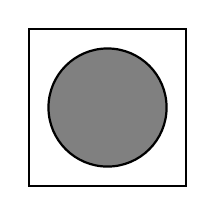
\begin{tikzpicture}
\draw[fill=white,thick](0,0) rectangle (2,2);
\draw[fill=gray,thick] (1,1) circle (0.75cm);
\end{tikzpicture}
\hspace{2cm}
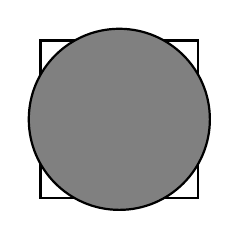
\begin{tikzpicture}
\draw[fill=white,thick](0,0) rectangle (2,2);
\draw[fill=gray,thick] (1,1) circle (1.15cm);
\end{tikzpicture}
\end{center}
\end{ans}
\newpage
\subsubsection{Section B}
\begin{qns}[Oscillation]
A mechanical model for a hydrogen atom in a varying external electric field $E(t)$ is shown in the picture below.
\begin{figure}[H]
    \centering
    \includegraphics[scale=0.5]{2011P1B6Q.PNG}
\end{figure}
\begin{enumerate}[label=(\roman*)]
\item The model consists of an electron of mass $m_e = 9.1\times 10^{−31}$ kg and charge $−e$, where $e = 1.6 × 10^{−19}$ C, connected to an infinitely massive proton via a spring of constant $k = 2.9$ N m$^{−1}$, which represents the electron–proton interaction, in parallel with a damper of constant $b = 5.7\times10^{-18}$ N s m$^{−1}$, which represents the losses due to radiation. Show that the displacement $x$ of the electron from its equilibrium position has the form \hfill\textbf{[2]}
$$\ddot{x}+\gamma\dot{x}+\omega_0^2x=-\frac{eE(t)}{m_e}$$
\item Calculate the values of $\omega_0$ and $\gamma$ for the Hydrogen atom.\hfill\textbf{[2]}
\item A beam of light incident on the atom is modelled as an oscillating electric field $E(t) = \text{Re}(E_0e^{i\omega t})$, where $\omega$ is the angular frequency of the radiation. Show that the velocity of the electron in this case is given by\hfill\textbf{[3]}
$$v=\text{Re}(v_0e^{i\omega t})$$
where
$$v_0=\frac{-i\omega E_0e}{m_e[(\omega_0^2-\omega^2)+i\gamma\omega]}$$
\item If the mean power absorbed by the atom is given by $\frac{1}{2}|b|v_0|^2$, show that the peak power absorption occurs for light waves at an angular frequency of $\omega_0$.\hfill\textbf{[3]}
\item Show that the bandwidth over which the power absorption is greater than half its maximum value is given by $\Delta\omega=\gamma$ (you may assume  $\gamma<<\omega_0$).\hfill\textbf{[4]}
\item Sketch a graph of the power absorption versus frequency for the model hydrogen  atom and give the wavelength of the peak and its width in nanometres.\hfill\textbf{[4]}
\item Describe qualitatively what happens if the model atom is in a constant electric field and the field is then instantaneously switched off, giving relevant timescales. \hfill\textbf{[2]}
\end{enumerate}
\end{qns}
\newpage
\begin{ans}\leavevmode
\begin{enumerate}[label=(\roman*)]
\item The equation of motion is $m_e\ddot{x}=-b\dot{x}-kx-eE(t)$. Set $\omega_0^2=k/m_e$, $\gamma=b/m_e$.
\item $\omega_0=\sqrt{\frac{2.9}{9.1\times10^{-31}}}=1.8\times10^{15}$ rad/s and $\gamma=\frac{5.7\times10^{-18}}{9.1\times10^{-31}}=6.2\times10^{12}$ N/m.
\item Set $x=\text{Re}[Ae^{i\omega t}]$, then $A=-\frac{eE_0}{m_e(\omega_0^2-\omega^2+i\omega\gamma)}$. We then differentiate $x$:
$$\dot{x}=\text{Re}\bigg[\frac{-i\omega eE_0e^{i\omega t}}{m_e(\omega_0^2-\omega^2+i\omega\gamma)}\bigg]=\text{Re}[v_0e^{i\omega t}]$$
\item The power is
$$P=\frac{1}{2}b|v|^2=\frac{1}{2}b\frac{\omega^2E_0^2e^2}{m_e^2[(\omega_0^2-\omega^2)^2+\omega^2\gamma^2]}=\frac{be^2E_0^2}{2m_e^2[\frac{(\omega_0^2-\omega^2)^2}{\omega^2}+\gamma^2]}$$
which is maximized when $\omega_0=\omega$, where $P_{max}=P(\omega=\omega_0)=\frac{be^2E_0^2}{2m_e^2\gamma^2}$.
\item At the half power points, i.e. $P=\frac{1}{2}P_{max}$:
$$\frac{be^2E_0^2}{2m_e^2[\frac{(\omega_0^2-\omega^2)^2}{\omega^2}+\gamma^2]}=\frac{be^2E_0^2}{4m_e^2\gamma^2}\implies\gamma\omega_\pm=\mp(\omega_0^2-\omega^2_\pm)$$
Adding them together give $\gamma(\omega_++\omega_-)=\omega_+^2-\omega_-^2=(\omega_+-\omega_-)(\omega_+-\omega_-)\implies\Delta\omega=\gamma$.
\item The quality factor is $Q=\frac{\omega_0}{\Delta\omega}=\frac{1.8\times10^{15}}{6.2\times10^{12}}=3.0\times10^2$, $\lambda_0=\frac{2\pi c}{\omega_0}=\frac{2\pi 3\times10^8}{1.8\times10^{15}}=1000\mu$ m, $\Delta\lambda=\frac{-2\pi c}{\omega^2\Delta\omega}=-\frac{2\pi 3\times10^8\times 6.2\times10^{12}}{(1.8\times10^{15})^2}=-3.6$ nm. The power absorption curve gives a sharp peak at $\lambda=\lambda_0$ and a full width half maximum of $\Delta\lambda$.

\begin{center}
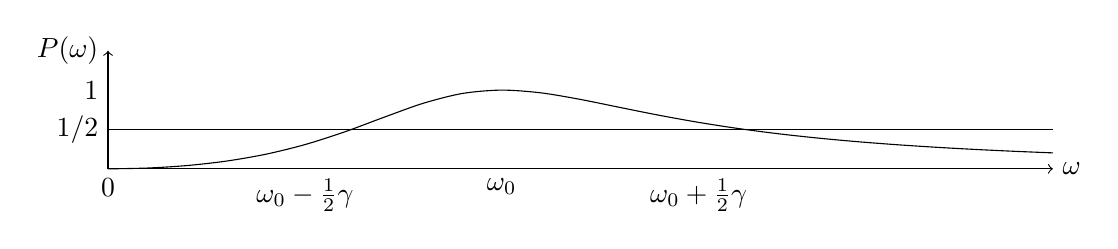
\begin{tikzpicture}
      \draw[->] (0,0) -- (12,0) node[right] {$\omega$};
      \draw[->] (0,0) -- (0,1.5) node[left] {$P(\omega)$};
      \draw[domain=0:12,smooth,variable=\x,black] plot ({\x},{(0.2*\x)^2/((1-(0.2*\x)^2)^2+(0.2*\x)^2)});
      \draw[domain=0:12,smooth,variable=\x,black] plot ({\x},{0.5});
      \draw (0,0) node[below]{0};
      %\draw 
%\foreach \x in {1,2,...,4} {%
    %\draw ($(\x,0) + (0,-\TickSize)$) -- ($(\x,0) + (0,\TickSize)$);
%}

\draw (0,1) node[left]{1};
\draw (0,1/2) node[left]{1/2};
\draw (2.5,0) node[below]{$\omega_0-\frac{1}{2}\gamma$};
\draw (5,0) node[below]{$\omega_0$};
\draw (7.5,0) node[below]{$\omega_0+\frac{1}{2}\gamma$};
\end{tikzpicture}
\end{center}
\item The system oscillates at $\omega_0$, and decays exponentially with a decay constant $\tau=\frac{1}{\gamma}=1.6\times10^{-13}$ s.
\end{enumerate}
\end{ans}
\newpage
\begin{qns}[Dispersion]\leavevmode
\begin{enumerate}[label=(\roman*)]
\item Under dispersive conditions, the \textit{group velocity} of a wave packet can be different from the \textit{phase velocity}. Explain with the aid of sketches the meaning of the italicised terms above.\hfill\textbf{[5]}
\item By considering the relative phases of different frequency components of a wave packet or otherwise, show that the group velocity $v_g$ is given by
$$v_g=\frac{\partial\omega}{\partial k}\bigg|_{\omega_0}$$
where $\omega$ is angular frequency, $k$ is wavenumber and $\omega_0$ is the central angular frequency of the packet. \hfill\textbf{[3]}
\item Surface waves in deep water obey the relation $\omega=\sqrt{gk}$, where $g$ is the acceleration due to gravity. Show that the group velocity is half the phase velocity for waves of any given frequency.\hfill\textbf{[2]}
\item A passenger on a ship sees that waves are approaching the ship in distinct groups. They observe that, at any instant, there are approximately 6 wave crests in all groups. The passenger now counts the number of crests that strike the ship in any one group and gets a significantly different number. Use sketches of a wave group and the ship in a frame in which the envelope of the wave group is at rest to explain why this is and calculate the typical number of crests counted in this case. You may assume that the ship is at rest on the ocean and there are no ocean currents.\hfill\textbf{[5]}
\item A wave monitor off the coast of Hawaii measures the typical periods of the waves arriving from the open ocean. One day, the monitor begins to record the arrival of waves coming from a distant ocean storm, and the dominant period is 20 s. A day later, the dominant period of the waves is 15 s. Using this information, estimate the distance to the storm from Hawaii, stating any assumptions you make.\hfill\textbf{[5]}
\end{enumerate}
\end{qns}
\begin{ans}\leavevmode
\begin{enumerate}[label=(\roman*)]
\item If we consider a superposition of lots of different frequency harmonic waves, we may localize the disturbance to produce a wavepacket. If the dispersion relation $\omega=\omega(k)$ is not linear, then the phase velocity $v_p=\frac{\omega}{k}$ is not constant for all waves. The phase velocity is the velocity at which the phase of a harmonic wave $\cos(kx-\omega t+\phi)=\cos(k(x-\frac{\omega}{k}t)+\phi)$ travels. The group velocity $v_g$ is the velocity at which interference features travel, most commonly chosen to be the velocity of the maximum amplitude. For positive dispersion, the higher frequency waves travel faster and the wavefronts bunch together at the front. For negative dispersion, the lower frequency waves travel faster, and so the wavefronts bunch together at the back.
\item Stationary phase approximation: $0=\frac{\partial}{\partial k}(kx-\omega t+\phi)=x-\frac{\partial\omega}{\partial k}t\implies v_g=\frac{x}{t}=\frac{\partial\omega}{\partial k}$.
\item $\omega=\sqrt{gk}$. The phase velocity is $v_p=\frac{\omega}{k}=\sqrt{g/k}$. The group velocity is $\frac{\partial\omega}{\partial k}=\frac{1}{2}\sqrt{\frac{g}{k}}=\frac{1}{2}v_p$.
\item In the rest frame of the packet, the individual wave crests moving at $v_g$, the ship is moving at $-v_g$. Let the length of the packet be $L$ such that $L/6$ is one wavelength. Then for the wavepacket to break in the ship, in this frame, it must move a distance $L$, which takes a time $T=\frac{L}{v_g}$. During this time, the phase velocity has caused the individual waves to move a distance $v_pT=12L$, and so a total of 12 crests reak on the ship.
\item The distance is equal to $v_g(\tau=20s)T$ and also equal to $v_g(\tau=15s)(T+1\text{day})$ where $\tau$ is the period $1/f$ of the wave while $T$ is the time taken it takes for the wave to reach from the source to the receiver. Longer period waves travel faster.\\[5pt]
We have $v_p^2=g/k=\frac{g\lambda}{2\pi}=\frac{g}{2\pi}\frac{v_p}{f}\implies v_p=\frac{g}{2\pi f}\implies v_g=\frac{g}{4\pi f}$. So, let $\tau=20$s,
$$\frac{g\tau}{4\pi}T=\frac{g(\tau-5)}{4\pi}(T+24\times 3600)\implies 1=\bigg(1-\frac{5}{\tau}\bigg)\bigg(1+\frac{24\times 3600}{T}\bigg)$$
which gives $T=2.59\times10^5$s and so the distance is $\frac{g\times 20}{4\pi}\times T$ to be $4.04\times10^6$ m. 
\end{enumerate}
\end{ans}
\newpage
\begin{qns}[Fraunhofer Diffraction]\leavevmode
\begin{enumerate}[label=(\roman*)]
\item Fraunhofer diffraction occurs when the phase change varies linearly with position across an aperture. For an aperture of width $d$ illuminated by plane waves with wavelength $\lambda$, show that the quadratic and higher order terms in the phase change can be neglected at a distance $D$, provided that\hfill\textbf{[5]}
$$D>>\frac{d^2}{\lambda}$$
\item An alternative way of observing Fraunhofer diffraction uses lenses to provide appropriate conditions. Sketch an optical configuration for observing Fraunhofer diffraction using a point source of light and two lenses.\hfill\textbf{[2]}
\item A parallel beam of light is incident normally on a diffraction grating which consists of a regular array of 200 narrow slits per mm, each slit being 1 $\mu$m wide. Light emerging from the grating is focussed by a lens of focal length 300 mm onto a screen. The lens and screen are centred on a line perpendicular to the centre of the grating, and are parallel to the grating. It is intended to observe the 3rd diffraction order with light at a wavelength of around 460 nm. Where on the screen does this diffraction order appear? \hfill\textbf{[2]}
\item Sketch the diffraction patterns of the grating when (a) the slit width is 1.0 $\mu$m, (b) the slit width is changed to 1.5 $\mu$m, but with the same centre-to-centre slit spacing, and keeping the same intensity in the incoming beam.\hfill\textbf{[4]}
\item Calculate the approximate changes in intensities of the 0th and 3rd diffraction orders between cases (a) and (b) above. \hfill\textbf{[3]}
\item The light illuminating the grating comes from a lamp emitting two equally bright narrow spectral lines at wavelengths of 459.5 nm and 460.0 nm respectively. Sketch the diffraction pattern around the 3rd grating order when the illuminating beam is (a) 5.0 mm wide (b) 1.5 mm wide (you may assume that the slit widths are small in this case, and that the grating is much wider than 5 mm). \hfill\textbf{[4]}
\end{enumerate}
\end{qns}
\begin{ans}\leavevmode
\begin{enumerate}[label=(\roman*)]
\item Consider a spherical source with strength $a_S$, at distance $s(x,y)$ from the aperture element $dxdy$ with overall aperture function $h(x,y)$. The incoming spherical wave have amplitude $\psi_1=a_Se^{iks}/s$, and the aperture element acts as a source of secondary wavelets with amplitude $-(i/\lambda)\psi_1(x,y)h(x,y)dxdy$. This secondary wave generates a disturbance at point P and have amplitude $d\psi_P$. Integrating everywhere gives us the total amplitude at point P, at a distance $r(x,y)$ from the aperture element
$$\psi_P=-\int\frac{i}{\lambda}h(x,y)K(\theta)\frac{a_Se^{ik(s+r)}}{sr}dxdy$$
where $K(\theta)$ is the obliquity factor to ensure momentum of photons is conserved. Consider the diffraction pattern in a plane at a distance $L$ from the aperture. We denote the coordinates of point P in this plane by $(x_0,y_0)$ and further assume P to be close to the axis. Assume that the source S is a large distance behind the aperture, and the aperture is illuminated with a plane wave at normal incidence.\\[5pt]
Considering P close to the axis such that $K=1$ and $x_0/L<<1$, $y_0/L<<1$, then the distance $r$ from the aperture element $dxdy$ to P is
$$r^2=L^2+(x_0-x)^2+(y_0-y)^2=D^2\bigg(1-2\frac{x_0x+y_0y}{D^2}+\frac{x^2+y^2}{D^2}\bigg)$$
where $D^2=L^2+x_0^2+y_0^2$. Using binomial expansion, we obtain $r\approx D-\frac{x_0x+y_0y}{D}+\frac{x^2+y^2}{2D}$. Since the phase of each wavelet is directly proportional to $kr$, the phase will have terms which vary linearly and quadratically with the position in the aperture. For large $D$, we obtain the Fraunhofer diffraction condition $\forall x,y\in\Sigma$, where we can drop the quadratic term and left with the linear term. Equivalently, for an aperture of maximum extent $d=\sqrt{x^2+y^2}$, the quadratic term for the phase $kr$ must be much less than $\pi$, i.e. $\frac{x^2+y^2}{2D}k<<\pi\implies D>>\frac{d^2}{\lambda}$. \item We can use lenses on either side of the aperture to convert the diverging beam from the source into a parallel beam, and to focus the diffracted parallel beams onto an observation screen. The source and observation screen must be placed at the object and image planes of the lenses, which are conjugate points. An aperture placed anywhere along the optical axis will produce a Fraunhofer diffraction pattern in the image plane.
\begin{figure}[H]
    \centering
    \includegraphics[scale=0.4]{fraunhoferlimit.PNG}
    \caption{Implementing Fraunhofer Diffraction}
\end{figure}
\item Using small angle approximation, $\sin\theta\approx\tan\theta=\frac{y}{f}$. For maxima we have $\frac{2\pi}{\lambda}d\sin\theta=2n\pi\implies2d\sin\theta=2n\lambda$. Hence, the position of the $n$th order on the screen is $y=\frac{n\lambda f}{d}=\frac{3(460\times10^{-9})(0.3)}{(5\times10^{-6})}=0.08$ m.
\item (a) $a/d=0.2$; (b) $a/d=0.3$. For (b), the width of the central lobe of the $\sinc^2$ envelope in the intensity plot is smaller, and we are likely to see less intense higher orders.
\item The ratio of intensity of the $n$th order to the zeroth order is
$$\frac{I(\theta(n))}{I(0)}=\bigg(\frac{\sin(0.5ka\sin\theta)}{0.5ka\sin\theta}\frac{\sin(0.5Nkd\sin\theta)}{N\sin(0.5kd\sin\theta)}\bigg)^2=\bigg(\frac{\sin(\chi0.5\pi n)}{0.5\chi\pi n}\frac{\sin(0.5N\chi\pi)}{N\sin(0.5\chi\pi)}\bigg)^2$$
where $n=3$, $\chi=0.2$ for (a) and $\chi=0.3$ for (b). Hence, the ratio of intensities of (a) to (b) is 0.737 to 0.488, about 1.5 times.
\item Illuminating only a finite region of the grating would be akin to having a $N=W/d$ slit grating. The positions of the third order are $y=\frac{3(0.3)}{2(5\times10^{-6})}\lambda$, which are 0.041355 and 0.0414 m (very close together!). The ratio of intensities are $\frac{\sin(4712)}{1000}\frac{300}{\sin(4.712\times 300)}=0.977$.
\end{enumerate}
\end{ans}
\newpage
\begin{qns}[Fabry-Pérot]\leavevmode
\begin{enumerate}[label=(\roman*)]
\item Define what is meant by the terms wave impedances $Z_1$ and $Z_2$ and reflection coefficient $r$ in the formula\hfill\textbf{[4]}
$$r=\frac{Z_1-Z_2}{Z_1+Z_2}$$
\item A monochromatic laser beam is incident normally on the surface of a parallel-sided sheet of silicon, with a refractive index of $n = 3.5$. Calculate the internal reflection coefficient $r$ for beams reflecting at a silicon–air interface (the impedance to electromagnetic waves for a material of refractive index $n$ is $\frac{Z_0}{n}$ where $Z_0$ is the impedance of free space).\hfill\textbf{[2]}
\item By considering the multiple internal reflections in the sheet, show that the intensity of the laser light transmitted through the sheet varies with wavelength as
$$I\frac{1}{|1-r^2e^{i\delta}|^2}$$
where $\delta=4\pi nd/\lambda$ with $\lambda$ the wavelength of the laser in air, $n$ the refractive index and $d$ the thickness of the sheet. You may use the result that $1+x+x^2+x^3+...=(1-x)^{-1}$ for $|x|<1$.\hfill\textbf{[5]}
\item If the sheet has a thickness of 1000 nm and the laser wavelength is tuned through the range 1200–1600 nm, at what wavelengths is the transmitted intensity at its maximum and minimum, and what is the ratio of the maximum to minimum transmitted intensity?\hfill\textbf{[5]}
\item Explain, with the aid of a sketch, how the variation of the transmission with wavelength would change if the sheet were covered on both faces with a coating with a high reflection coefficient.\hfill\textbf{[4]}
\end{enumerate}
\end{qns}
\begin{ans}\leavevmode
\begin{enumerate}[label=(\roman*)]
\item Consider a wave with complex amplitude $Ae^{i(kx-\omega t)}$, then the impedance $Z$ in a medium is the ratio of the `force' to the appropriate velocity response of the medium. For instance, tension to transverse velocity for a wave in a string, ratio of $H$ field to $E$ field in an electromagnetic wave.\\[5pt]
The amplitude reflection coefficient $r$ for a wave propagating from region 1 to region 2 is the ratio of the amplitude of outgoing wave in region 1 to the incoming wave in region 1.
\item $r=\frac{(1/3.5)-1}{(1/3.5)+1}=\frac{1-3.5}{1+3.5}=-\frac{2.5}{4.5}=\frac{-5}{9}$.
\item At each interface, light is either transmitted with transmission amplitude coefficient $t_{12}$ or $t_{21}$, or reflected. On passing through the sheet, the ray must be transmitted exactly once through each boundary, but must be reflected an even number of times.\\[5pt]
The optical path difference between consecutive rays will be $2d\cos\theta$, and so each round trip acquires a phase difference of $\delta=\frac{2\pi}{\lambda'}2d$, where $\lambda'=\frac{\lambda}{\pi}$ is the wavelength of the light in the medium. The final amplitude $A$ is thus related to the initial amplitude $A_0$ by
$$A=A_0t_{12}t_{21}e^{i\delta}+A_0t_{12}t_{21}e^{i\delta}r^2_{21}e^{i\delta}+A_0t_{12}t_{21}e^{i\delta}(r^2_{21}e^{i\delta})^2+...=\frac{A_0t_{12}t_{21} e^{i\delta}}{1-r_{21}^2e^{i\delta}}$$
The transmitted intensity is thus
$$I=|A|^2=\frac{|A_0|^2|t_{12}t_{21}|^2}{|1-r^2e^{i\delta}|^2}\propto\frac{1}{|1-r^2e^{i\delta}|^2}$$
\item As $r=r^*$, $\frac{I}{I_0}=\frac{1}{(1-r^2e^{i\delta})(1-r^2e^{-i\delta})}=\frac{1}{1+r^4-2r^2\cos\delta}$. Then, the maximum and minimum values are $\frac{1}{(1-r^2)^2}$ and $\frac{1}{(1+r^2)^2}$ for $\delta=2p\pi$ and $\delta=(2p+1)\pi$, for $p\in\mathbb{Z}$. Since, $\delta=\frac{4\pi nd}{\lambda}$, we must have $p=\frac{2nd}{\lambda}$. For the shortest wavelength $\lambda_1=1200$ nm, we have $$\frac{2(3.5)(1000\times10^{-9})}{1200\times10^{-9}}=5.88$$
For the longest wavelength $\lambda_1=1600$ nm, we have $$\frac{2(3.5)(1000\times10^{-9})}{1600\times10^{-9}}=4.375$$
In this range, we have a maximum when $p=5$, then the wavelength is $\lambda=\frac{2n d}{p}=\frac{2}{5}\times 1000\times10^{-9}=1.4\mu$m. When $\lambda=\frac{4nd}{2p+1}$, we have 1.56 $\mu$m and 1.27 $\mu$m, for $n=9$ or 11 respectively. Edge cases do not matter for global extrema. The ratio of maximum to minimum intensity will be $(\frac{1+r^2}{1-r^2})^2$.
\item With the highly reflective coatings, $|r|\rightarrow 1$, hence the peaks will be sharper and the valleys in between will be broader and deeper. Since by continuity, we must have $t_{12}=1+r_{12}$, and so $t_{12}t_{21}=(1+r_{12})(1+r_{21})=1-r_{12}^2$. Then, the intensity will be
$$I=|A_0|^2\frac{(1-r^2)^2}{1+r^4-2r^2\cos\delta}$$
with maximum value $|A_0|^2$ and minimum $|A_0|^2=\frac{(1-r^2)^2}{(1+r^2)^2}$. In the plot, $r$ for the blue curve is greater than that of the red curve.
\begin{center}
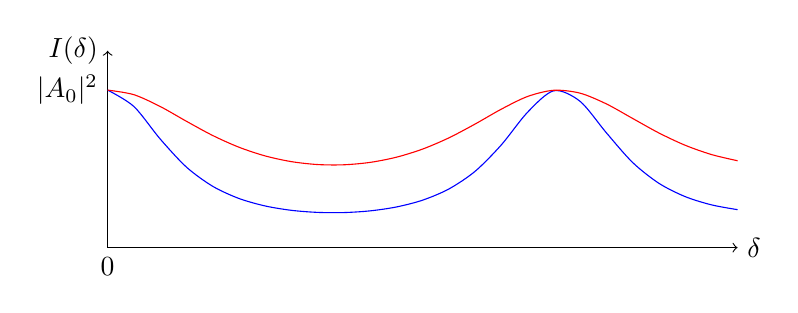
\begin{tikzpicture}
      \draw[->] (0,0) -- (8,0) node[right] {$\delta$};
      \draw[->] (0,0) -- (0,2.5) node[left] {$I(\delta)$};
      \draw[domain=0:8,smooth,variable=\x,blue] plot ({\x},{2*(1-0.6^2)^2/(1+0.6^4-2*0.6^2*cos(20*pi*\x))});
    \draw[domain=0:8,smooth,variable=\x,red] plot ({\x},{2*(1-0.4^2)^2/(1+0.4^4-2*0.4^2*cos(20*pi*\x))});
      \draw (0,0) node[below]{0};
    \draw (0,2) node[left]{$|A_0|^2$};
\end{tikzpicture}
\end{center}
\end{enumerate}
\end{ans}
\newpage
\subsubsection{Section C}
\begin{qns}[Scattering]\leavevmode
\begin{enumerate}[label=(\roman*)]
\item State the energy and momentum conservation laws that govern the interaction of a particle with a crystal structure, (a) for elastic processes, and (b) for inelastic processes,
which involve phonon absorption (annihilation) or creation. \hfill\textbf{[4]}
\item Neutrons of mass $m_n = 1.67 \times 10^{−27}$ kg, with momentum $\hbar k_i$ and energy $E=\frac{\hbar^2k_i^2}{2m_n}$, scatter from a crystal by absorbing phonons of energy $\hbar\omega$ and crystal momentum $\hbar q$. All of the momentum change is perpendicular to the momentum of the incident neutrons. Show that energy and momentum conservation are satisfied, if $\hbar\omega=\hbar^2q^2/2m_n$. \hfill\textbf{[4]}
\item The dispersion relation of the absorbed phonons can be modelled as
$$\omega=\frac{2v}{a}\bigg|\sin\bigg(\frac{qa}{2}\bigg)\bigg|$$
where $v = 2000$ m s$^{−1}$ and $a = 0.5$ nm. Show that $\pi/a<q<2\pi/a$.\hfill\textbf{[4]}
\item Using a linear approximation to the phonon dispersion relation in the range $\pi/a<q<2\pi/a$ or otherwise, estimate the wavevector and frequency of the absorbed phonons.\hfill\textbf{[5]}
\item Explain why the neutrons are no longer scattered in this way when the crystal is cooled to very low temperature.\hfill\textbf{[3]}
\end{enumerate}
\end{qns}
\begin{ans}\leavevmode
\begin{enumerate}[label=(\roman*)]
\item Say the particle has energy $E_i, E_f$ and momentum $\mathbf{k_i}, \mathbf{k_f}$ before and after the collision respectively, and the phonon has energy $E$ and momentum $\mathbf{q}$, and the crystal has reciprocal lattice vectors $\mathbf{G_{hkl}}$, then
\begin{itemize}
    \item for elastic processes, no phonons are created, so $E_i=E_f+\hbar\omega$, but $\mathbf{k_f}-\mathbf{k_i}=\mathbf{G_{hkl}}$ for some $\mathbf{G_{hkl}}$ as the crystal centre of mass must change momentum. The centre of mass momentum of crystals is represented (due to Nyqusit) by $\hbar$ times the integer numbers of reciprocal lattice vectors.
    \item For inelastic processes, $\mathbf{k_f}-\mathbf{k_i}=\pm\mathbf{q}+\mathbf{G_{hkl}}$ and $E_f-E_i=\pm E'$ for creation and annihilation respectively.
\end{itemize}
\item The energy of the photon is $\hbar\omega=\frac{\hbar^2}{2m_n}(k_f^2-k_i^2)$ while the momentum is $\mathbf{q}=\mathbf{k_f}-\mathbf{k_i}$ where $\mathbf{q}\cdot\mathbf{k_i}=0$, so $k_f^2=|\mathbf{k_i}+\mathbf{q}|^2=k_i^2+q^2$. Hence, $\omega=\frac{\hbar q^2}{2m_n}$.
\item We numerically solve
$$\frac{\hbar a}{4 v m_n}q^2=\bigg|\sin\frac{qa}{2}\bigg|$$
but $\sin\frac{\pi}{a}\frac{a}{2}=1$, so evaluate the left at $q=\frac{\pi}{a}$
$$\frac{\hbar a}{4m_nv}\frac{\pi^2}{a^2}=\frac{(6.626\times10^{-34}/2\pi)0.5\times10^{-9}\pi^2}{4(1.67\times10^{-27})2000(0.5\times10^{-9})^2}=0.156<1$$
So looking at the intersection graphically, we must have $\frac{\pi}{a}<q<\frac{2\pi}{a}$.
\item Let $\alpha:=\frac{\hbar a}{4m_nv}$, we now solve
$$\alpha q^2=\pi-\frac{qa}{2}\implies q=\frac{1}{2\alpha}(-0.5a+\sqrt{0.25a^2+4\alpha\pi})$$
where the positive root gives $1.1\times10^{10}m^{-1}$, which give an energy $\frac{\hbar^2q^2}{2m_n}=2.5\times10^{-3}$eV. 
\item At low temperatures, the phonons required to be annihilated just do not exist since they are too energetic to be present due to thermal motion, hence this process does not occur.

\end{enumerate}
\end{ans}
\newpage
\begin{qns}[Heat Capacity]\leavevmode
\begin{enumerate}[label=(\roman*)]
\item State general expressions in the form of $k$-space sums or energy integrals for the contributions to the internal energy of a metal from (a) conduction electrons, (b) lattice vibrations. Explain the terms in your expressions.\hfill\textbf{[5]}
\item Explain, without detailed mathematical derivations, why 
\begin{enumerate}[label=(\alph*)]
    \item the electronic contribution, $C_{el}$, to the molar heat capacity of metals at low temperature, $T$, is proportional to $T$ and proportional to the density of states at the Fermi energy, $g(E_F)$;\hfill\textbf{[5]}
    \item the lattice contribution, $C_{la}$, to the molar heat capacity of metals at low temperature is proportional to $T^3$, and why it tends to a constant at temperatures larger than the Debye temperature $\theta_D$.\hfill\textbf{[6]}
\end{enumerate}
\item Given that
$$C_{el}(T)\approx 3k_B^2g(E_F)T,\quad C_{la}(T)=\frac{12\pi^4}{5}R\bigg(\frac{T}{\theta_D}\bigg)^3$$
for potassium, $\theta_D=$ 100 K and the Fermi energy, $E_F$, is 2 eV, estimate the temperature at which the lattice and electronic contributions to the molar heat capacity are equal for potassium.\hfill\textbf{[4]}
\end{enumerate}
\end{qns}
\begin{ans}\leavevmode
\begin{enumerate}[label=(\roman*)]
\item The density of states for particles of momentum $p=\hbar|\mathbf{k}|$ is
$$g(p)dp=\frac{4\pi p^2dp}{h^3/V}$$
\begin{enumerate}[label=(\alph*)]
\item Since electrons are fermions, they obey the Fermi-Dirac probability distribution
$$p_{FD}(\epsilon)=\frac{1}{\exp[(\epsilon-\mu)/k_BT]+1}$$
where $\mu$ is the chemical potential, which is approximately equal to the Fermi energy for temperatures much less than the melting temperature. As electrons are massive particles, we have $\epsilon=\frac{p^2}{2m}\implies d\epsilon=\frac{pdp}{m}$ and so the internal energy $U$ is
$$U=\int_0^\infty\epsilon p_{FD}(\epsilon)g(\epsilon)d\epsilon=\frac{8\pi V}{h^3}\int_0^{\infty}\frac{\epsilon^{3/2}d\epsilon}{\exp[(\epsilon-\mu)/k_BT]+1}$$
\item Phonons on the other hand are bosons, they obey the Bose-Einstein probability distribution
$$p_{BE}(\epsilon)=\frac{1}{\exp[(\epsilon-\mu)/k_BT]-1}$$
and so the internal energy is 
$$U=\int_0^{\epsilon_{max}}\epsilon p_{BE}(\epsilon)g(\epsilon)d\epsilon$$
The finite upper limit $\epsilon_{max}$ occur since phonons have a fixed number of modes. Phonons have spin 1 and hence 3 polarization state. $g(\epsilon)$ generally has a complicated form, but it has to account for different values of $\frac{\partial\omega}{\partial\mathbf{q}}$ in different directions.
\end{enumerate}
\item 
\begin{enumerate}[label=(\alph*)]
\item Since the constituent particles of a metal obey Fermi-Dirac statistics, only the electrons within $k_BT$ of the Fermi energy have empty states that they can be excited to. Thus, the internal energy can be approximated as the number of electrons that can be excited $g(\epsilon_F)k_BT$ multiplied by the energy of each electron $k_BT$, i.e.
$$U_{\text{el}}\sim k_BT g(\epsilon_F)k_BT$$
so the electronic contribution to the heat capacity is $C_{\text{el}}=\frac{\partial U_{\text{el}}}{\partial T}=2k_B^2Tg(\epsilon_F)$.
\item At low temperatures, we have a linear dispersion relation for phonons, i.e. $\omega(\mathbf{q})=v_s|\mathbf{q}|$ where $v_s$ is the speed of sound in the crystal. This means $p^2dp=\frac{\epsilon^2}{v_s^3}d\epsilon$ and so we approximate the Bose Einstein distribution as $p_{BE}(\epsilon)\approx e^{-\epsilon/k_BT}$. We approximate the upper limit of the internal energy as as infinity, i.e.
$$U_{\text{la}}\sim\int_0^\infty\epsilon e^{-\epsilon/k_BT}3\frac{4\pi\epsilon^2}{v_s^3}d\epsilon$$
The evaluated integral has a $T^4$ behaviour and thus the lattice contribution to the heat capacity is $C_{\text{la}}\sim T^3$. This approximation is valid at $T<<\theta_D$ for some characteristic temperature $\theta_D$. But if $T>>\theta_D$, all $3N$ modes have been excited since by equipartition theorem, each of the 6 degrees of freedom has $\frac{1}{2}k_BT$, so $C_{\text{la}}\sim 3k_BT$. In reality, finding $\theta_D$ requires knowledge of the form of $\omega(\mathbf{q})$ but with a quick estimation, it yields $\theta_D\propto n^{1/2}v_s$ where $n=N/V$.
\end{enumerate}
\item Solve for $T$ where $C_{el}=C_{la}$
$$3k_B^2g(\epsilon_F)T=\frac{12}{5}\pi^4R\frac{T^3}{\theta_D^3}\implies T^2=\frac{5k_B^2\theta_D^3}{4\pi^4R}g(E_F)$$
The total number of modes should be $N_A$ (one mole) 
$$N_A=\int_0^{\epsilon_F}K\epsilon^{1/2}d\epsilon=K\frac{2}{3}\epsilon_F^{3/2}\implies K=\frac{3N_A}{2\epsilon_F^{3/2}}$$
So we have the molar density of states to be $g_M(\epsilon)=\frac{3N_A}{2\epsilon_F}$ and hence
$$T=\sqrt{\frac{15N_Ak_B^2\theta_D^3}{8\pi^4RE_F}}=\sqrt{\frac{15(1.38\times10^{-23})(100)^3}{8\pi^42(1.6\times10^{-19})}}=0.911K$$
which is very low.
\end{enumerate}
\end{ans}
\newpage
\subsubsection{Section D}
\begin{qns}[OWO Short Notes]
Write brief notes on two of the following:\hfill\textbf{[20]}
\begin{itemize}
    \item Fourier transform spectroscopy;
    \item resolution in imaging instruments;
    \item the dispersion relation for guided waves.
\end{itemize}
\end{qns}
\begin{ans}\leavevmode
\subsubsection*{Fourier transform spectroscopy:}
To understand Fourier transform spectroscopy, we first discuss the setup of the Michelson interferometer. The beam-splitter splits the incident beam with components travel along different paths, and recombine at the same beam-splitter. Constructive or destructive interference will occur depending on the difference between the two paths. Normally, one path is kept fixed (reference path) and the other path is varied by moving a mirror (on a precision stage) in order to see a fringe pattern as a function of the mirror position. This arrangement focuses the beams onto a photodiode. The system is illuminated with the collimated beam; the mirrors are aligned so that the path difference is constant across the beam\\[5pt]
For an extended light source, light from different parts of the source travels at different angles through the interferometer to the eye and the differential delays will be a function of this angle. Mirrors may also be tilted to introduce different delays for beams hitting the mirrors at different points. The combination of these effects means that a spatially-varying intensity (i.e. fringes) can be seen when the mirrors are both held fixed.
\begin{figure}[H]
    \centering
    \includegraphics[width=\linewidth]{mmi.PNG}
\end{figure}
Consider the following example. A Fourier Transform Spectrograph has a maximum mirror displacement of $\Delta x=50$ cm. What is its spectral resolution at a wavelength of $\lambda_0=1\mu$m?\\[5pt]
We measure the Fourier transform $I(x)$ of the source spectrum $S(k)$ but over a limited range of $x$ values. The maximum pathlength difference is 1 m. Assume that this is disposed symmetrically about the position of zero pathlength difference, i.e. $x$ ha a range $\pm50$cm. The measured intensity $I'(x)$ over this range is equal to $I(x)$ over infinite limits multiplied by a tophat function $W(x)$ of width $w=2\Delta x=1$m, i.e. $I'(x)=W(x)I(x)$. The reconstructed spectrum $S'(k)$ is the convolution, i.e. $S'(k)=\mathcal{F}(W)(k)*S(k)$ . Spectral information at finer resolutions is lost. The width of the blurring function ($\mathcal{F}(W)(k)$ is sinc) in spatial frequency space is $\Delta k=\frac{2\pi}{w}$. We find that $\frac{|\Delta\lambda|}{\lambda}=\frac{\Delta k}{k}=\frac{\lambda}{w}$. So the spectral resolving power $\frac{\lambda}{\Delta\lambda}=10^6$ in this case. We can distinguish spectral lines which are 1 pm apart when the central wavelength is 1 $\mu$m.\\[5pt]
Note that by Nyquist Criterion, the sampling rate $\Delta x$ must be high enough so that copies of the source spectrum do not overlap. Hence, the bandwidth $\Delta k$ must obey $\Delta k<\frac{\pi}{\Delta x}\implies\Delta x<0.5\lambda_{min}$. Clearly, the maximum separation between points on the wavefront sets the spectral resolution. The bigger the separation, the better the resolution.
\begin{figure}[H]
    \centering
    \includegraphics[width=\linewidth]{FTS.PNG}
\end{figure}
\subsubsection*{Resolution in imaging instruments:}
We will be discussing resolution in the context of two imaging instruments, namely the typical diffraction grating and the Fabry-Pérot etalon. To determine two spectral lines are resolved, we use the Rayleigh criterion. Rayleigh Criterion states that two lines can only be resolved from each other if at their minimum separation, the maximum of one line lies over the first zero of the other.\\[5pt]
Consider a diffraction grating with slit spacing $d$ being used to analyze a spectrum. The limit of resolution is determined by looking for the highest order, and then imposing the Rayleigh criterion. The $m$th order maximum will be when $\Delta\phi=2\pi m$. For the longer of the two wavelengths $\lambda_2$ we set the angle to $\theta=0.5\pi$ to discover the maximum order:
$$2\pi m=\Delta\phi=\frac{2\pi}{\lambda_2}d\sin\frac{\pi}{2}$$
We then require the first zero after the $m$th maximum of the other wavelength, $\lambda_1$ to also be at $\theta=0.5\pi$. This occurs when $\Delta\phi=2\pi m+\frac{2\pi}{N}$ and so
$$\frac{2\pi}{\lambda_1}d\sin\frac{\pi}{2}=\frac{2\pi}{N}+2m\pi\implies\lambda_1^{-1}-\lambda_2^{-1}=(Nd)^{-1}\implies Nd=\frac{\lambda_1}{\lambda_2-\lambda_1}d$$
The greater the number of slits/lines $N$, the higher the resolving power. Wider gratings give narrower diffraction beams which are easier to distinguish. It is also easier to distinguish wavelengths at higher order, since upon fixing widths, their angular separation increases with $m$. At any given angle, a number of different wavelengths may satisfy the diffraction condition, corresponding to different orders. It is necessary to use filters to remove higher order diffractions in order to obtain an accurate spectrum from a broadband source.\\[5pt]
Consider a film of air (of thickness $d$) sandwiched between two mirrors, known as a Fabry-Pérot etalon. A fraction $t$ of this beam is transmitted in passing from glass to air, and a further fraction $t'$ transmitted in passing from air to glass, giving an emerging beam of amplitude $tt'=T$. This etalon produces a fringe pattern with much sharper features than a simple thin film, and is useful for high resolution spectroscopy. Each successive beam emerging from the etalon acquires a factor of $R:=r^2$ in amplitude and a phase shift $\delta$, where $\delta=\frac{4\pi d}{\lambda}\cos\theta$ (thin film). The fringe pattern has maxima at $\delta=\frac{4\pi d}{\lambda}\cos\theta=2m\pi$ for $m\in\mathbb{Z}^+$. At normal incidence $\theta=0$ we have an integer number of half wavelengths between the mirrors.
\begin{figure}[H]
    \centering
    \includegraphics[scale=0.8]{2019P2B6.PNG}
\end{figure}
The sharpness of the peaks is a function of $\delta$. The maximum value of $\frac{I_{out}}{I_{in}}=\frac{T^2}{(1-R)^2}$ where $\delta=2m\pi$. We define the half-width of the peaks $\delta_{1/2}$ as the change in $\delta$ required for the intensity to reduce to half its maximum value.
$$\frac{4R}{(1-R)^2}\sin^2(0.5\delta_{1/2})=1\implies\delta_{1/2}\approx\frac{1-R}{\sqrt{R}}$$
It is useful to define the finesse, $\mathcal{F}$ as the ratio of separation of successive peaks in $\delta$ (equal to $2\pi$) to their full-width at half maximum $(2\delta_{1/2})$
$$\mathcal{F}=\frac{2\pi}{2\delta_{1/2}}=\frac{\pi\sqrt{R}}{1-R}$$
The finesse is a measure of the quality of the etalon and becomes high as $R\rightarrow 1$. The chromatic resolving power of the etalon is defined as $\frac{\lambda}{\Delta\lambda}$.
$$d\delta=-\frac{4\pi d\cos\theta}{\lambda^2}d\lambda\implies|d\delta|:=\Delta\delta=\frac{\delta}{\lambda}\Delta\lambda=2\delta_{1/2}\implies\frac{\lambda}{\Delta\lambda}=\frac{2\pi d\cos\theta}{\lambda\delta_{1/2}}$$
Since $2d\cos\theta=m\lambda$ at maxima, the resolving power is $\frac{\lambda}{\Delta\lambda}=\frac{m\pi}{\delta_{1/2}}=m\mathcal{F}$. This has the same form as the resolving power in the $m$th order for a diffraction grating of $N$ lines, where $N_{eff}$ is $\mathcal{F}$ of the Fabry-Pérot interferometer. This effective number is also the number of interfering beams in the interferometer.
\newpage
\subsubsection*{The dispersion relation for guided waves:}
Consider an effective model for guided waves: waves on a large 2D elastic membrane in the $xy$ plane. The membrane is clamped along $y=0$ and $y=b$ and hence $k_y$ is quantized, i.e. $k_y=\frac{n\pi}{b}$, where $n\in\mathbb{Z}^+$. The constituent waves are multiply reflected at the boundaries with a phase change of $\pi$ radians at each as they move down the guide. The dispersion relation is $$v^2\nabla^2\psi=\frac{\partial^2\psi}{\partial t^2}\implies\omega^2=v^2(k_x^2+\frac{n^2\pi^2}{b^2})$$ 
If we were to superpose the two waves before and after a reflection, we have
$$Ae^{i(\omega t-k_xx-k_yy)}-Ae^{i(\omega t-k_xx+k_yy)}=Ae^{i(\omega t-k_xx)}[e^{-ik_yy}-e^{ik_yy}]=-2iA\sin(k_yy)e^{i(\omega t-k_xx)}$$
The wave travelling in the $x$ direction has amplitude modulated by the standing wave in the $y$ direction. A cutoff frequency exists since for $\omega<\frac{n\pi v}{b}:=\omega_c$, $k_x<0$ and so propagation is not possible. Here, the wave is evanescent. If a spread of frequencies exist, multiple modes can be excited and the signal will distort. The waveguide is single-moded if only one mode is excited.\\[5pt]
If we have different modes propagating, the signal output at any given time will be superimposed, the time-delayed copies of different input signals can be mitigated in three ways:
\begin{itemize}
    \item choose physical dimensions such that for frequency range of interest, where only one mode can propagate;
    \item undo the distortion in software later;
    \item choose the physical dimension such that for the frequency range of interest, many modes can be activated. Very little power will be injected into the high $n$ modes and most will go into modes already in the linear regime where $\omega\approx vk$ and so exhibit no dispersion.
\end{itemize}
The phase velocity is $$v_p=\frac{\omega}{k_x}=\frac{\omega}{\sqrt{(\omega/v)^2-(n\pi/b)^2}}$$
and the group velocity is obtained by $$2\omega\frac{d\omega}{dk_x}=2v^2k_x\implies v_pv_g=v^2\implies v_g=\frac{v^2}{\omega^2}\sqrt{(\omega/v)^2-(n\pi/b)^2}$$
The phase velocity $v_p=\frac{v}{\cos\theta}$ is greater than $v$. $v_p$ travels at an angle $\theta$ inclined to the $x$-axis while $v$ is along the $x$-axis. Note that $\tan\theta=k_y/k_x$. The wavelength of the guided wave $\lambda_x$ is thus longer than the unguided wave $\lambda$. We also have 
$$\lim_{k_x\rightarrow\infty}v_p,v_g=v\quad\lim_{k_x\rightarrow0}v_g=0\quad\lim_{k_x\rightarrow0}v_p=\infty$$
but this does not violate special relativity since the energy is transmitted at $v_g$, which is less than $v=c$.\\[5pt]
An optical fibre, an example of a waveguide, comprises a cylindrical silica core, surrounded by a cladding of lower refractive index. Optical waves can be guided down the core of the fibre. The data is sent as a series of pulses of light, and the data rate which can be achieved over a given length of fibre is determined by the spreading out of these pulses as they are transmitted along the fibre, i.e. by the dispersion.\\[5pt]
The opposing effects of the waveguide dispersion relation and $n(\lambda)$ of glass can minimize unwanted dispersion in optical fibres. Hence, choose a wavelength with minimal dispersion such that losses in this wavelength is kept small as well.\\[5pt]
Propagation of light in more than one mode would therefore lead to major pulse spreading, hence most fibres are designed with a core which is sufficiently small that only one propagating mode exists.
\end{ans}
\newpage
\begin{qns}[CMP Essay]
Explain qualitatively, with the aid of energy band diagrams, the operation of (a) rectifying diodes, (b) light emitting diodes, and (c) photovoltaic cells, all based on semiconductor p−n junctions.\hfill\textbf{[20]}
\end{qns}
\begin{ans}
Adding dopants that gives more (fewer) electrons than the substrate itself creates an n-type (a p-type) semiconductor. At non-zero temperatures, all these states are ionized, increasing the conductance of the material. For the n-type (p-type), the vast majority of the charge carriers are ionized electrons (holes left behind when electrons from the filled band were excited into the dopant hole state). In the absence of impurities, the Fermi energy ($\mu(T=0)$) is in the middle of the band gap. When the donor (acceptor) impurities are added, at zero temperature, impurity states near the top (bottom) of the bandgap are filled (empty). The Fermi energy is moved up to the top (down to the bottom) of the band gap.\\[5pt]
Although the n-doped system has free negatively charged electrons and the p-doped system has free positively charged holes, both systems are overall electrically neutral since charged ions compensate for the charges of the mobile charge carriers. When the two doped semiconductors are brought into contact, the electrons in the conduction band will fall into the valence band, filling the empty hole states, thus pair-annihilating both the electron and the hole. This amounts to a gain in energy of $E_{gap}$ per pair annihilated. After this process of electrons falling into holes and annihilating occurs there will be a region near the interface where there are no free carriers at all. This is the depletion region, which is electrically charged (since there are charged ions but no carriers to neutralize them). Hence, there is a net electric field pointing from the positively charged to the negatively charged ions. This is a p-n junction.\\[5pt]
(a) \textbf{Rectifying diodes:} In a rectifying diode, current is only allowed to flow through the junction easily in one direction, but not the other. There are 4 processes that can create current:
\begin{enumerate}
    \item Electrons may be thermally excited into the conduction band. Some of these electrons will flow down the slope to the left.
    \item Holes may be thermally excited down into the valence band and will flow up the slope to the right. 
    \item Electrons in the conduction band on the left will be thermally activated to climb up the potential slope in the depletion layer and will annihilate with holes once they arrive at the p-doped side. 
    \item Holes in the valence band on the right may be thermally activated to climb down the potential slope towards the n-doped side where they annihilate with electrons.
\end{enumerate}
The contribution by processes 1 and 2 to the current is directly proportional to $e^{-E_{gap}/k_BT}$. Voltage bias will not change the number of excited carriers, hence current independent of voltage.\\[5pt]
The contribution by processes 3 and 4 to the current is directly proportional to $e^{-E_{gap}/k_BT}$ in the absence of an applied voltage, and $e^{-(E_{gap}+eV)/k_BT}$ in the presence of an applied voltage. The total current flow will be the sum and hence
$$I=J_s(T)(e^{-eV/k_BT}-1)$$
where $J_s$ is directly proportional to $e^{-E_{gap}/k_BT}$ is known as the saturation current. This is the diode equation. Current flows easily in one direction, i.e. forward biased, but flows poorly in the opposite direction, i.e. reverse biased.
\begin{figure}[H]
    \centering
    \includegraphics[width=\linewidth]{biasedPN.PNG}
    \caption{Band diagram of a biased p-n junction. The four processes that can create current are labelled. In the absence of applied voltage, the net current is zero. When voltage is applied, current flows easily for $eV<0$ and not easily with $eV>0$.~\cite{simon2013oxford} }
\end{figure}
(b) \textbf{Light emitting diodes:} A light emitting diode is a p-n junction that is optimized for the production of photons during carrier recombination. To induce light emission, we forward bias the p-n junction. The majority of the carriers flow into the junction and recombine, releasing energy. In a direct bandgap material, light emission can be the most favourable process. The size of the bandgap determines the wavelength of the photons emitted. LEDs are widely used, including in communications and in efficient lighting.\\[5pt]
(c) \textbf{Photovolatic cells:} If one applies light to a semiconductor, electron-hole pairs may be excited if the energy of a photon is greater than the energy of the bandgap. In most regions of the semi-conductor, the created electrons and holes will quickly annihilate upon exposure to light. However, in the depletion region, due to the electric field in this region, electrons which are created flow off towards the n-doped region and holes which are created flow off towards the p-doped region. In both cases, the charge current is moving to the right.
\end{ans}
\newpage
\subsection{Paper 2}
\subsubsection{Section A}
\begin{qns}[1D Potential]
A one-dimensional potential, V(x), with value zero at the origin, has an eigenfunction $\psi\propto e^{-ax^4}$. Find the form of the potential and the energy of the eigenstate. 

\hfill\textbf{[4]}
\end{qns}
\begin{ans}
Since $\psi\propto e^{-ax^4}$, $\psi'\propto -4ax^3\psi$ and $\psi''\propto (-12ax^3+16a^2x^6)\psi$, then the Schrodinger equation gives
$$-\frac{\hbar^2}{2m}4ax^2(-3+4ax^4)\psi=(E-V)\psi$$
Since $V(x=0)=0$, then $E=0$ $\forall x$. Hence, $V=\frac{2\hbar^2}{m}ax^2(4ax^4-3)$.
\end{ans}
\begin{qns}[1D Potential]
A particle moves in the potential shown in the diagram. The energy of the fourth lowest bound state is indicated. Sketch the corresponding wavefunction.\hfill\textbf{[4]}
\begin{figure}[H]
    \centering
    \includegraphics[scale=0.5]{2011P2A2Q.PNG}
\end{figure}
\end{qns}
\begin{ans}
The wavefunction is the fourth lowest bound state, so third excited state, hence three nodes. $E-V>0$ within the well so $\psi$ is oscillatory, but for regions where $E-V$ is smaller (shallower well), $k=\frac{\sqrt{2m(E-V)}}{\hbar}$ is smaller, hence the wavelength of oscillation is larger. The converse is true. Since $E-V<0$ outside of the well, $k\notin\mathbb{R}$ and $\psi$ must be an exponential decay.
\end{ans}
\begin{qns}[Misc]
For a one-dimensional quantum mechanical system, show that $[\hat{p}_x^2,\hat{x}]=-2i\hbar\hat{p}_x$, where $\hat{p}_x$ and $\hat{x}$ are the momentum and position operators. \hfill\textbf{[4]}
\end{qns}
\begin{ans}
With $[\hat{x},\hat{p}_x]=i\hbar$,
$$[\hat{p}_x^2,\hat{x}]=\hat{p}_x[\hat{p}_x,\hat{x}]+[\hat{p}_x,\hat{x}]\hat{p}_x=-2i\hbar\hat{p}_x$$
\end{ans}
\begin{qns}[Error Analysis]
If
$$z=\frac{\tan(x+y)}{\tan(x)}$$
with $x = 20\degree\pm 4\degree$ and $y = 30\degree\pm 3\degree$, estimate the value of $z$ and its error.\hfill\textbf{[4]}
\end{qns}
\begin{ans}
$z=\frac{\tan(50\degree)}{\tan(20\degree)}=3.274$. The error in $z$ is approximately
$$\sigma_z^2\approx\bigg(\frac{\partial z}{\partial x}\bigg)^2\sigma_x^2+\bigg(\frac{\partial z}{\partial y}\bigg)^2\sigma_y^2=\bigg(\frac{\sec^2(x+y)}{\tan(x)}-\frac{\tan(x+y)}{\sin^2(x)}\bigg)^2\sigma_x^2+\bigg(\frac{\sec^2(x+y)}{\tan(x)}\bigg)^2\sigma_y^2=0.18176$$
which gives $\sigma_z\approx 0.4$, so $z=3.3\pm0.4$.
\end{ans}
\begin{qns}[Sampling]
An analogue to digital converter quantizes an input voltage which is randomly distributed, with a standard deviation very much larger than $\Delta V$, the spacing of the digitised levels. Show that the r.m.s. of the difference between the input and the digitised output is $\Delta V/\sqrt{12}$.\hfill\textbf{[4]}
\end{qns}
\begin{ans}
We can treat the input signal as uniform over the range since its standard deviation is larger than the spacing of the digitized levels. Our probability distribution is relative to the trigger level: $p(x)=\frac{1}{\Delta V}$, $|x|\leq\frac{\Delta V}{2}$ and 0 elsewhere. By symmetry, $\overline{x}=0$ but $\overline{x^2}\neq 0$.
$$\overline{x^2}=\int_{-\Delta V/2}^{\Delta V/2}\frac{x^2}{\Delta V}dx=\bigg[\frac{x^3}{3\Delta V}\bigg]^{\Delta V/2}_{-\Delta V/2}=\frac{(\Delta V)^2}{12}$$
hence the r.m.s difference is $\Delta V/\sqrt{12}$.
\end{ans}
\newpage
\subsubsection{Section B}
\begin{qns}[Hybrid]\leavevmode
\begin{enumerate}[label=(\roman*)]
\item A particle of mass $m$ can undergo isotropic simple harmonic oscillation in the $x$−$y$ plane, characterised by the oscillation frequency $\omega$. The lowering and raising ladder operators are defined by
$$\hat{a}_x=\sqrt{\frac{m\omega}{2\hbar}}\hat{x}+i\frac{\hat{p}_x}{\sqrt{2m\omega\hbar}}\text{  and   }\hat{a}_x^\dag=\sqrt{\frac{m\omega}{2\hbar}}\hat{x}-i\frac{\hat{p}_x}{\sqrt{2m\omega\hbar}}$$
respectively, where $\hat{x}$ and $\hat{p}_x$ are the position and momentum operators corresponding to motion in direction $x$, with similar operators defined for motion in direction $y$. The quantum numbers for energy eigenstates in directions $x$ and $y$ are $k$ and $l$ respectively, so a particular quantum state is designated $|k\rangle |l\rangle$. Derive the Hamiltonian for this system in terms of the ladder operators.\hfill\textbf{[4]}
\item State the effect of the following operations on the specified states, including the usual normalisation:\hfill\textbf{[3]}
$$\hat{a}_x|k\rangle|l\rangle,\quad\hat{a}_y^\dag|k\rangle|l\rangle,\quad\hat{a}_z|0\rangle|l\rangle$$
\item Show that the operator $\hat{L}_z$ corresponding to orbital angular momentum about the direction $z$ can be expressed as, \hfill\textbf{[5]}
$$\hat{L}_z=-i\hbar(\hat{a}_x^\dag\hat{a}_y-\hat{a}_y^\dag\hat{a}_x)$$
\item and demonstrate that $\hat{L}_z$ is a constant of the motion.\hfill\textbf{[4]}
\item Show that the state
$$\Psi=|1\rangle|0\rangle+i|0\rangle|1\rangle$$
is an eigenfunction of $\hat{L}_z$, and determine the corresponding angular momentum.\hfill\textbf{[4]}
\end{enumerate}
\end{qns}
\begin{ans}\leavevmode
\begin{enumerate}[label=(\roman*)]
\item The Hamiltonian for a 2D isotropic harmonic oscillator is
$$\hat{H}=\frac{1}{2m}
(\hat{p}_x^2+\hat{p}_y^2)+\frac{1}{2}m\omega^2(\hat{x}^2+\hat{y}^2)$$
We will only work out the operators associated with $x$, since the algebra for $y$ is similar. We have $\hat{x}=\sqrt{\frac{\hbar}{2m\omega}}(\hat{a}_x+\hat{a}_x^\dag)$ and $\hat{p}_x=i\sqrt{\frac{m\omega\hbar}{2}}(\hat{a}_x^\dag-\hat{a}_x)$. To proceed further, we evaluate
$$[\hat{a}_x,\hat{a}_x^\dag]=\sqrt{\frac{m\omega}{2\hbar}}\frac{-i}{\sqrt{2m\omega\hbar}}2[\hat{x},\hat{p}_x]=1$$
Then, $\hat{x}^2=\frac{\hbar}{2m\omega}(\hat{a}-x^2+(\hat{a}_x^\dag)^2+2\hat{a}_x^\dag\hat{a}-x+1)$ and $\hat{p}_x^2=-\frac{m\omega\hbar}{2}((\hat{a}_x^\dag)^2+\hat{a}_x^2-2\hat{a}_x^\dag\hat{a}-x-1)$. The Hamiltonian is
$$\hat{H}_x=\frac{1}{2m}(\hat{p}_x^2)+\frac{1}{2}m\omega^2\hat{x}^2=\frac{1}{2}\hbar\omega+\hbar\omega\hat{a}_x^\dag\hat{a}_x$$
Thus, the Hamiltonian is $\hat{H}=\hbar\omega(\hat{a}_x^\dag\hat{a}_x+\hat{a}_y^\dag\hat{a}_y+1)$.
\item $\hat{a}_x|k\rangle|l\rangle=\sqrt{k}|k-1\rangle|l\rangle$, $\hat{a}_y^\dag|k\rangle|l\rangle=\sqrt{l+1}|k\rangle|l+1\rangle$ and $\hat{a}_x|0\rangle|l\rangle=0$.
\item Classically, $L_z=xp_y-yp_x$, so
$$\hat{L}_z=\hat{x}\hat{p}_y-\hat{y}\hat{p}_x=\sqrt{\frac{\hbar}{2m\omega}}(\hat{a}_x+\hat{a}_x^\dag)i\sqrt{\frac{m\omega\hbar}{2}}(\hat{a}_y^\dag-\hat{a}_y)-\sqrt{\frac{\hbar}{2m\omega}}(\hat{a}_y+\hat{a}_y^\dag)i\sqrt{\frac{m\omega\hbar}{2}}(\hat{a}_x^\dag-\hat{a}_x)=-i\hbar(\hat{a}_x^\dag\hat{a}_y-\hat{a}_x\hat{a}_y^\dag)$$
To show that $\hat{L}_z$ is a constant of motion, we invoke Ehrenfest theorem.
$$\frac{d\langle\hat{L}_z\rangle}{dt}=\frac{i}{\hbar}\langle[\hat{H},\hat{L}_z]\rangle+\bigg\langle\frac{\partial\hat{L}_z}{\partial t}\bigg\rangle=0+0=0$$
where the commutator with the Hamiltonian $[\hat{H},\hat{L}_z]$ is
$$[\hbar\omega(\hat{a}_x^\dag\hat{a}_x+\hat{a}_y^\dag\hat{a}_y+1),-i\hbar(\hat{a}_x^\dag\hat{a}_y-\hat{a}_x\hat{a}_y^\dag)]=-i\hbar^2\omega([\hat{a}_x\hat{a}_x^\dag,\hat{a}_x^\dag]\hat{a}_y-[\hat{a}_x\hat{a}_x^\dag,\hat{a}_x]\hat{a}_y^\dag+\hat{a}_x^\dag[\hat{a}_y^\dag\hat{a}_y,\hat{a}_y]-\hat{a}_x[\hat{a}_y^\dag\hat{a}_y,\hat{a}_y^\dag])=0$$
where we used $[\hat{a}\hat{a}^\dag,\hat{a}^\dag]=\hat{a}^\dag$ and related identities.
\item The eigenvalue of $\psi$ is $+\hbar$ and so $m_z=+1$.
$$\hat{L}_z\psi=i\hbar(|0\rangle|1\rangle+i0|2\rangle-|2\rangle0-i|1\rangle|0\rangle)=\hbar(i|0\rangle|1\rangle+|1\rangle)\\rangle)$$
For a 2D system, the total angular momentum just consists of that in the $z$-component. Hence, it is just $\hbar$.
\end{enumerate}
\end{ans}
\begin{qns}[Hybrid]\leavevmode
\begin{enumerate}[label=(\roman*)]
\item What is meant by the term stationary state in quantum mechanics?\hfill\textbf{[3]}\\[5pt]
Conservation of probability implies that
$$\boldsymbol{\nabla}\cdot\mathbf{j}=-\frac{\partial\rho}{\partial t}$$
where $\rho=\psi^*\psi$ is the probability density corresponding to a wavefunction $\psi$, and $\mathbf{j}$ represents a probability current.
\item By using the time-dependent Schrödinger equation and its complex conjugate, show that probability conservation implies that there is a probability current $\mathbf{j}$ in a stationary state, for a particle of mass $m$, given by\hfill\textbf{[7]}
$$\mathbf{j}=\frac{\hbar}{2im}(\psi^*\boldsymbol{\nabla}\psi-\psi\boldsymbol{\nabla}\psi^*)$$
\item Derive the probability current in the normalized state
$$\psi=Are^{-r/2a_0}\sin\theta e^{i\phi}$$
at a point $(r, \theta, \phi)$ in spherical polar coordinates, where $A=1/(8\sqrt{\pi}a_0^{5/2})$.\hfill\textbf{[5]}
\item The product of probability current and mass is expected to describe linear momentum in an element of volume, and contributes $mrj\sin\theta dV$ to the angular momentum in the $z$-direction. Using this, calculate the total angular momentum in the $z$-direction in the given state.\hfill\textbf{[5]}
\end{enumerate}
\begin{mdframed}
\color{darkblue}{You may use the results $\int_0^\infty r^ne^{-r/a_0}dr=n!a_0^{n+1}$ and $\int_0^\pi\sin^3\theta d\theta=4/3$.}
\end{mdframed}
\end{qns}
\begin{ans}\leavevmode
\begin{enumerate}[label=(\roman*)]
\item A stationary state has a probability density that is time-independent, i.e. $\frac{\partial}{\partial t}|\psi|^2=0$, so any time-dependence of $\psi$ will ahve to appear in an overall phase factor. THis stationary state is an eigenstate of the Hamiltonian $i\hbar\frac{\partial}{\partial t}$ with a real eigenvalue (energy).
\item Using the result from conservation of probability,
$$\boldsymbol{\nabla}\cdot\mathbf{j}=-\frac{\partial}{\partial t}\psi^*\psi=-\psi\frac{\partial\psi^*}{\partial t}-\psi^*\frac{\partial\psi}{\partial t}=-\psi\frac{\hbar}{2im}\nabla^2\psi^*+\psi^*\frac{\hbar}{2im}\nabla^2\psi$$
But $\nabla^2f=\boldsymbol{\nabla}\cdot(\boldsymbol{\nabla}f)$ for some scalar function. Thus, we get the desired form of $\mathbf{j}$ with $\mathbf{j}=\boldsymbol{0}$ when $\psi=0$.
\item In spherical polar,
$$\boldsymbol{\nabla}\psi=A\sin\theta e^{i\phi}\frac{\partial re^{-r/2a_0}}{\partial r}\mathbf{\hat{r}}+Are^{-r/2a_0}e^{i\phi}\frac{1}{r}\frac{\partial\sin\theta}{\partial\theta}\boldsymbol{\hat{\theta}}+Are^{-r/2a_0}\sin\theta\frac{1}{r\sin\theta}\frac{\partial e^{i\phi}}{\partial\phi}\boldsymbol{\hat{\phi}}$$
$$\boldsymbol{\nabla}\psi^*=A\sin\theta e^{-i\phi}\frac{\partial re^{-r/2a_0}}{\partial r}\mathbf{\hat{r}}+Are^{-r/2a_0}e^{-i\phi}\frac{1}{r}\frac{\partial\sin\theta}{\partial\theta}\boldsymbol{\hat{\theta}}+Are^{-r/2a_0}\sin\theta\frac{1}{r\sin\theta}\frac{\partial e^{-i\phi}}{\partial\phi}\boldsymbol{\hat{\phi}}$$
Thus, $\mathbf{J}=\frac{\hbar}{2mi}2i|A|^2re^{-r/a_0}\sin\theta\boldsymbol{\hat{\phi}}=\frac{\hbar}{m}\frac{1}{64\pi a^5}re^{-r/a_0}\sin\theta\boldsymbol{\hat{\phi}}$.
\item Conceptually, $\psi$ will obviously have eigenvalue $\hbar$ when $\hat{L}_z$ acts on it. To check:
$$\int mrj\sin\theta dV=\int mr^2\frac{\hbar}{m}\frac{e^{-r/a_0}\sin^2\theta}{64\pi a_0^5}r^2\sin\theta d\theta d\phi=\frac{\hbar}{64\pi a_0^5}\int_0^\infty r^4e^{-r/a_0}dr\int_0^\pi\sin^3\theta d\theta\int_0^{2\pi}d\phi$$
where we used the hinted integrals to get $\frac{\hbar}{64\pi a_0^5}4!a_0^5\frac{4}{3}2\pi=\hbar$.
\end{enumerate}
\end{ans}
\begin{qns}[Spin]
Electrons in a particular solid possess a magnetic dipole moment, $\hat{\boldsymbol{\mu}}$, related to their intrinsic spin, $\hat{\mathbf{S}}=\frac{\hbar}{2}\hat{\boldsymbol{\sigma}}$, by $\hat{\boldsymbol{\mu}}=(ge/2m)\hat{\mathbf{S}}$ , where $g$ is the Landé g-factor for the electron in this system, and $\hat{\boldsymbol{\sigma}}$ is a vector of Dirac matrices, with components
$$\hat{\sigma}_x=\begin{pmatrix}0&1\\1&0\\\end{pmatrix},\quad\hat{\sigma}_y=\begin{pmatrix}0&-i\\i&0\\\end{pmatrix},\quad\hat{\sigma}_z=\begin{pmatrix}1&0\\0&-1\\\end{pmatrix}$$
\begin{enumerate}[label=(\roman*)]
\item Construct the Hamiltonian $\hat{H}=-\hat{\boldsymbol{\mu}}\cdot\mathbf{B}$ for an electron in a uniform magnetic flux density $\mathbf{B} = (B_x, B_y, B_z)$.\hfill\textbf{[4]}\\[5pt]
Eigenstates of angular momentum in the $z$-direction are denoted
$$\begin{pmatrix}1\\0\\\end{pmatrix}\text{   and   }\begin{pmatrix}0\\1\\\end{pmatrix}$$
corresponding to $S_z =+\hbar/2$ and $S_z=-\hbar/2$ respectively. The solid is located in a region of uniform magnetic flux density $\hat{B}_x$ in the x-direction, and the electrons are prepared in the state denoted  
$$\begin{pmatrix}1\\0\\\end{pmatrix}$$
\item By considering the time-dependent Schrödinger equation, show that the expression for the state is in the form\hfill\textbf{[6]}
$$\psi=\cos(\omega t)\begin{pmatrix}1\\0\\\end{pmatrix}+i\sin(\omega t)\begin{pmatrix}0\\1\\\end{pmatrix}$$
\item The spin of the electrons can be measured at a time $t$ after the initial preparation of the state.
\begin{enumerate}[label=(\alph*)]
    \item Show that the expectation value of the spin measured in the x-direction is zero at all times.\hfill\textbf{[4]}
    \item  Show that the expectation value of the spin measured in the $z$-direction varies as $\cos(\Omega t)$, find an expression for $\Omega$, and give a physical interpretation of this time dependence.\hfill\textbf{[6]}
\end{enumerate}
\end{enumerate}
\end{qns}
\begin{ans}\leavevmode
\begin{enumerate}[label=(\roman*)]
\item Write the Hamiltonian as
$$\hat{H}=-\hat{\boldsymbol{\mu}}\cdot\mathbf{B}=-\frac{ge}{2m}\frac{\hbar}{2}\boldsymbol{\hat{\sigma}}\cdot\boldsymbol{\hat{B}}=-\frac{ge\hbar}{4m}
\begin{pmatrix}B_z&B_x-iB_y\\B_x+iB_y&-B_z\\\end{pmatrix}$$
\item The field is only in the $x$-direction, so we need to solve the Schrodinger equation:
$$i\hbar\frac{\partial}{\partial t}
\begin{pmatrix}a\\b\\\end{pmatrix}=-\frac{ge\hbar}{4m}\begin{pmatrix}0&B_x\\B_x&0\\\end{pmatrix}\begin{pmatrix}a\\b\\\end{pmatrix}$$
We get a coupled first order differential equation $\dot{a}=\frac{igeB_x}{4m}b$ and $\dot{b}=\frac{igeB_x}{4m}a$, which is basically one second order differential equation $\ddot{a}=-\frac{g^2e^2}{16m^2}a$. Together with the initial condition $\psi(t=0)=(1,0)^T$, the solution is $\psi(t)=(\cos\omega t,i\sin\omega t)^T$ where $\omega=\frac{ge}{4m}B_x$.
\item For both parts evaluate matrix equation.
\begin{enumerate}[label=(\alph*)]
\item $\langle\hat{S}_x\rangle=\langle\psi(t)|\frac{\hbar}{2}\hat{\sigma}_x|\psi(t)\rangle=0$
\item $\langle\hat{S}_z\rangle=\langle\psi(t)|\frac{\hbar}{2}\hat{\sigma}_z|\psi(t)\rangle=\frac{\hbar}{2}(\cos^2\omega t-\sin^2\omega t)=\frac{\hbar}{2}\cos(2\omega t)$. Thus, $\Omega=2\omega$. The state behaves like a vector, rotating in an abstract 2D space. The basis of this space is the eigenvectors that correspond to these two observables. To jump into an eigenstate with probability 1 would require that the state is either aligned or anti-aligned with the basis state. The probabilities of getting the desired eigenstates happen at twice the frequency of the rotation.
\end{enumerate}
\end{enumerate}
\end{ans}
\newpage
\begin{qns}[Central Potential]\leavevmode
\begin{enumerate}[label=(\roman*)]
\item In some circumstances the motion of an electron, mass $\mu$, about a massive fixed positive particle of charge $+e$, can be confined to two dimensions. Show that in this case, with a Coulomb interaction of the form $V(r)=-\frac{e^2}{4\pi\epsilon_0r}$, the Schrödinger equation for the electron has a separable solution $\psi(r,\phi)=R(r)\Phi(\phi)$ which leads to a radial equation of the form\hfill\textbf{[5]}
$$r\frac{d^2R}{dr^2}+\frac{dR}{dr}+\bigg[\frac{2\mu}{\hbar^2}\bigg(Er+\frac{e^2}{4\pi\epsilon_0}\bigg)-\frac{m^2}{r}\bigg]R=0$$
\item Explain why $m$ should be an integer.\hfill\textbf{[2]}\\[5pt]
To solve this equation for bound states, a further substitution is made, of the form $R(r) = G(x)x^me^{−x/2}$, with
$$r=xN\frac{2\pi\hbar^2\epsilon_0}{\mu e^2}\text{  and   }E=-\frac{\mu e^4}{32\hbar^2\pi^2\epsilon_0^2N^2}$$
\item The function $G(x)$ can be shown to satisfy
$$x\frac{d^2G}{dx^2}+(2m+1-x)\frac{dG}{dx}+(N-m-0.5)G=0$$
Show that the relation between successive terms in the power series for\hfill\textbf{[6]}
$$G(x)=\sum_{n=0}a_nx^n$$
is
$$a_{n+1}=a_n\frac{m+n+0.5-N}{(n+1)(2m+n+1)}$$
\item By considering the termination of the power series deduce what values can be taken by $N$.

\hfill\textbf{[3]}
\item Compare the sequence of energies of the lowest three bound states in this two-dimensional case to that of the corresponding three-dimensional system.\hfill\textbf{[4]}
\end{enumerate}
\begin{mdframed}
\color{darkblue}{In two dimensional polar coordinates $(r,\phi)$,
$$\nabla^2=\frac{1}{r}\frac{\partial}{\partial r}\bigg(r\frac{\partial}{\partial r}\bigg)+\frac{1}{r^2}\frac{\partial^2}{\partial\phi^2}$$
}
\end{mdframed}
\end{qns}
\newpage
\begin{ans}\leavevmode
\begin{enumerate}[label=(\roman*)]
\item The Schrodinger equation for the Hydrogen atom is
$$-\frac{\hbar^2}{2\mu}\nabla^2\psi(r,\phi)-\frac{e^2}{4\pi\epsilon_0r}\psi(r,\phi)=E(r,\phi)$$
Using separation of variables, we have
$$-\frac{\hbar^2}{2\mu}\bigg(rR\bigg(\frac{dR}{dr}+r\frac{d^2R}{dr^2}\bigg)+\frac{1}{r^2\Phi}\frac{d^2\Phi}{d\phi^2}\bigg)=E+\frac{e^2}{4\pi\epsilon_0r}$$
Let $\frac{d^2\Phi}{d\phi^2}=-m^2\Phi$, then we recover the desired equation.
\item For $\Phi(\phi)$ to be single-valued, i.e. $\Phi(\phi+2\pi)=\Phi(\phi)$, $m$ needs to be an integer (that is not zero). In this case, $\Phi(\phi)=Ae^{im\phi}+Be^{-im\phi}$.
\item Using series solution
$$\sum_{n=0}na_nx^n+(2m+1)\sum_{n=0}na_nx^{n-1}-\sum_{n=0}a_nnx^n+(N-m-0.5)\sum_{n=0}a_nnx^n=0$$
Comparing coefficients for $x^n$, we get the recurrence relation.
\item We need $|\psi|^2$ to be normalizable. This requires $G(x)$ to terminate, i.e. polynomial. Thus, $N=m+n+0.5$, for some $n\geq0$, i.e. $N$ must be half-integer.
\item The energy is
$$E_{n,m,2D}=\frac{-\mu e^4}{32\pi^2\hbar^2\epsilon_0^2}\frac{1}{(m+n+0.5)^2}$$
\begin{itemize}
    \item Lowest bound state: $n=m=0$, $E_{00}=-\frac{\mu e^4}{8\hbar^2\pi^2\epsilon_0^2}$;
    \item Second lowest bound state: $n=1$, $m=0$ or vice-versa, $E_{01}=E_{10}=-E_{00}\frac{1}{9}$;
    \item Third lowest bound state: $n=1=m$, $n=2$, $m=0$ or vice-versa, $E_{02}=E_{20}=E_{11}=-E_{00}\frac{1}{25}$. 
\end{itemize}
Compared to the 3D energy spectrum $E_{n,3D}=-\frac{\mu e^4}{32\hbar^2\pi^2\epsilon_0^2}\frac{1}{n^2}$. The 2D energy levels are higher due to the energy associated with confining the electrons to a plane.
\end{enumerate}
\end{ans}
\newpage
\subsubsection{Section C}
\begin{qns}[QM Short Notes]
Write an essay on `The concept and consequences of indistinguishability'.\hfill\textbf{[20]}
\end{qns}
\begin{ans}
In classical mechanics, when a system is made of identical particles, it is possible to identify and distinguish each particle from the others. In quantum mechanics, however, identical particles are truly indistinguishable since we cannot specify more than a complete set of commuting observables, and due to uncertainty principle (path of a particle is meaningless).\\[5pt]
As an example, when scattering two identical particles in the centre of mass frame, it is impossible to forecast with certitude that the particle fired from source $S_1$ will make it to detector 1 or 2. 
\begin{figure}[H]
    \centering
    \includegraphics[width=\linewidth]{indistinguishable.PNG}
    \caption{Scattering of Indistinguishable Particles}
\end{figure}
Consider two particles with single particle basis $|\alpha\rangle$ and $|\beta\rangle$ respectively. We define the transposition operator
$$P_{12}|\alpha\rangle|\beta\rangle:=|\beta\rangle|\alpha\rangle$$
where $|\alpha\rangle|\beta\rangle=|\alpha\rangle\otimes|\beta\rangle$. Note $P_{12}\in\mathcal{L}(V\otimes V)$. The transposition operator is Hermitian, i.e. $P_{12}^\dag=P_{12}$. The eigenvalues of $P_{12}$ are $\pm1$, where $+1$ represents symmetric states and $-1$ represents anti-symmetric states.\\[5pt]
The spin-statistics theorem states that particles whose spin is an integer (half odd integer) multiple of $\hbar$ are described by totally symmetrical (anti-symmetric) states. They are bosons (fermions) and satisfy the Bose-Einstein (Fermi-Dirac statistics). Moreover, partially symmetric states do not exist. Essentially, for a system of $N$ identical particles,
$$P_{ij}|N\text{ identical bosons }\rangle=+|N\text{ identical bosons }\rangle$$
$$P_{ij}|N\text{ identical fermions }\rangle=-|N\text{ identical fermions}\rangle$$
where $P_{ij}$ is the permutation operator that interchanges the $i$th and the $j$ th particles, with $i$ and $j$ arbitrary.\\[5pt]
Consider two particles with states they can occupy be $|\alpha\rangle$ and $|\beta\rangle$. For bosons, the independent states are
$$|\alpha\rangle|\alpha\rangle,\quad|\beta\rangle|\beta\rangle,\quad\frac{1}{\sqrt{2}}(|\alpha\rangle|\beta\rangle+|\beta\rangle|\alpha\rangle)$$
For fermions, the only independent state can be written as
$$\frac{1}{\sqrt{2}}(|\alpha\rangle|\beta\rangle-|\beta\rangle|\alpha\rangle)$$
For classical particles (distinguishable), they follow the Maxwell-Boltzmann statistics. the independent states are $|\alpha\rangle|\beta\rangle$, $|\beta\rangle|\alpha\rangle$, $|\alpha\rangle|\alpha\rangle$, $|\beta\rangle|\beta\rangle$.\\[5pt]
For any two fermions, say if $\alpha=\beta$, the state vanishes, i.e. no such state exists. This is called Pauli Exclusion Principle, which states that no two fermions can occupy the same state.\\[5pt]
We generalize this to $N$ identical particles. For a system of many identical particles, we can define
$$P_{ij}|k^1\rangle|k^2\rangle...|k^i\rangle|k^{i+1}\rangle...|k^j\rangle...:=|k^1\rangle|k^2\rangle...|k^j\rangle|k^{i+1}\rangle...|k^i\rangle...$$
It is clear that $P_{ij}^2=1$ and the allowed eigenvalues are $\pm 1$ as well. Also, $[P_{ij},P_{kl}]\neq 0$. The normalization is $\sqrt{\prod_{i=1}^nN_i!/N!}$ where $N$ is the total number of particles and $N_i$ is the number of times $|k^{(i)}\rangle$ occurs. For $N$ particle systems, we can define $N!$ permutation operators. To build an anti-symmetric $N$ particle states, we use the Slater determinant (determinant ensures exchange of any two particles will give a minus sign).\\[5pt]
The total wavefunction may be written as a product of spatial $\psi(\mathbf{r_i})$ and spin wavefunction $\chi(\mathbf{m_{s_i}})$. We denote it as $|\Psi\rangle\in V\otimes W$, where $V$ and $W$ are spaces for spatial and spin states respectively. The overall state must satisfy the symmetrization postulate. Say if the overall state must be antisymmetric, then either spatial or the spin state must be symmetric, with the other being antisymmetric.
\end{ans}
\newpage
\begin{qns}[QM Essay]
Write brief notes on two of the following topics in quantum mechanics:\hfill\textbf{[20]}
\begin{itemize}
    \item the consequences of the non-commutation of operators;
    \item examples of tunnelling;
    \item singlet and triplet states.
\end{itemize}
\end{qns}
\begin{ans}\leavevmode
\subsubsection*{The consequences of the non-commutation of operators:}
Every observable of a physical system is associated with a Hermitian operator with a complete set of eigenfunctions. The (projective) measurement of an observable A may be represented formally by the action of the corresponding operator $\mathbf{\hat{A}}$ on a state vector $|\psi(t)\big\rangle$. If the measurement yields a quantum state $|\psi_n\big\rangle$, then the corresponding eigenvalue of this quantum state is $a_n$.\\[5pt]
$a_n$ is the component of $|\psi(t)\big\rangle$ when projected onto the eigenvector $|\psi_n\big\rangle$ using the projection operator where $a_n=\big\langle\psi_n|\psi(t)\big\rangle$. By Born's rule, the probability of measuring the quantum system to be in the state $|\psi_n\big\rangle$ is 
$$P_n=\frac{|\big\langle\psi_n|\psi\big\rangle|^2}{\big\langle\psi|\psi\big\rangle}=|\big\langle\psi_n|\psi\big\rangle|^2=|a_n|^2$$
After the measurement, the state of the system will be $|\psi_n\big\rangle$  and we can thus say that the wavefunction has collapsed or projected into the measured state. Note that the outcome of a single round of measurement is intrinsically unpredictable.\\[5pt]
The expectation value $\big\langle\mathbf{\hat{A}}\big\rangle$ represents the average result of measuring $\mathbf{\hat{A}}$ on the state $|\psi\big\rangle$. Heuristically, the expectation value can be regarded as a long-run mean. As we repeatedly measure the quantity A, the mean of this huge set of measurements will approach the expectation value. The expectation of the operator $\mathbf{\hat{A}}$ is
$$\langle\mathbf{\hat{A}}\rangle=\frac{\langle\psi|\mathbf{\hat{A}}|\psi\rangle}{\langle\psi|\psi\rangle}$$
The uncertainty of a random variable is the standard deviation - the square root of the expected value of the square of deviations from the average value. The uncertainty, by convention, is always more or equal to zero. Evidently, the eigenstate for a generic Hermitian operator $\mathbf{\hat{A}}$ has zero uncertainty.\\[5pt]
Two observables are said to be compatible if their operators commute and have a common basis of eigenstates. Their eigenvalues are good quantum numbers. Conversely, if the two observables are not compatible or equivalently, their operators do not commute, then we will not be able to simulataneously measure both observables. The Heisenberg Uncertainty relation for two generic incompatible observables, which are represented by the  Hermitian operators $\mathbf{\hat{A}}$ and $\mathbf{\hat{B}}$ respectively is
$$\sigma_A^2\sigma_B^2\geq\bigg|\frac{1}{2i}\big\langle[\mathbf{\hat{A}},\mathbf{\hat{B}}]\big\rangle\bigg|^2$$
Since they are incompatible, the operators do not commute. Suppose we define $\sigma_A^2\equiv\big\langle f|f\big\rangle$ and $\sigma_B^2\equiv\big\langle g|g\big\rangle$, then by Schwarz inequality,
$\big\langle f|f\big\rangle\big\langle g|g\big\rangle\geq|\big\langle f|g\big\rangle|^2$. 
$\big\langle f|g\big\rangle$ is thus
$$\big\langle f|g\big\rangle=\big\langle\psi|\mathbf{\hat{A}}\mathbf{\hat{B}}|\psi\big\rangle-\big\langle\mathbf{\hat{A}}\big\rangle\big\langle\mathbf{\hat{B}}\big\rangle\implies\text{Im}(\big\langle f|g\big\rangle)=\frac{1}{2i}(\big\langle f|g\big\rangle-\big\langle g|f\big\rangle)=\frac{1}{2i}\big\langle[\mathbf{\hat{A}},\mathbf{\hat{B}}]\big\rangle$$
We thus obtain our desired relation. For example, the uncertainty relation for position and momentum is 
$$\sigma_x\sigma_p\geq\frac{\hbar}{2}$$
where the canonical commutator relation can be shown to be $[\mathbf{\hat{x}},\mathbf{\hat{p}}]=i\hbar$. Hence, we cannot measure simultaneously both the position and momentum of any quantum system. Another example would be the non-commutation of any two angular momentum operators in distinct directions
$$[J_i,J_j]\neq0$$
This implies we cannot determine all three components of angular momentum simultaneously.
\subsubsection*{Examples of tunnelling:}
For a potential barrier of $U>0$, the probability for a particle of energy $E$ to transmit across the barrier is
$$P_{tr}=\frac{|J_{tr}|}{|J_{inc}|}=\frac{|T|^2}{|I|^2}=\frac{1}{1+\frac{U^2\sinh^2\kappa a}{4E(U-E)}}$$
This is the phenomenon of quantum tunnelling where there is non-zero probability of passing through the barrier even though it classically does not have enough energy. For $\kappa a>>1$, the probability decays as $e^{-2\kappa a}$. Next, we proceed to discuss a few experimental evidences of quantum tunnelling.\\[5pt]
Under normal circumstances, a low-energy electron cannot leave the surface of a metal because of the Coulombic interaction between the electron and the ions that make up the lattice.
The presence of an external electric field ($V =-Ex$) creates a potential having the form of a narrow barrier. Electrons can tunnel across this barrier giving rise to a process known as field emission. This process has been developed into the scanning tunneling microscope (STM).\\[5pt]
In the STM, a sharp tip is scanned over the surface the sample, and a voltage is applied such that field emission occurs. The tunneling current, which is exponentially dependent on spacing, is used to hold the tip at a fixed height above the surface. The feedback control to the piezo displacer is then used as a measure of the height of the surface.\\[5pt]
Another evidence is in radioactive decay. Large unstable nuclei can decay via the emission of an $\alpha$-particle, which is the nucleus of a He atom comprising two protons and two neutrons. The energy of the emitted $\alpha$-particle is small (4-9 MeV) compared with the nuclear barrier (20-25 MeV). The transmission probability, and therefore the rate of escape, depends near-exponentially on the kinetic energy of the released particle. Small changes in the energy of the released particle correspond to very large changes in the materials half life. A high-energy particle has a small half life.\\[5pt]
A similar example would be nuclear fusion in stars. Proton-proton chain rapidly occurs between positively-charged protons despite the large Coulomb barrier. This is because tunneling may occur, allowing a reaction to take place despite not having sufficient energy to overcome the Coulomb barrier, i.e. the star is not hot enough.
\newpage
\subsubsection*{Singlet and triplet states:}
To understand singlet and triplet states, we must first understand how to add angular momentum. When we combine states $|j_1,m_1\rangle$ and $|j_2,m_2\rangle$ each of which has definite angular momentum, the `obvious' basis of $H_{j_1}\otimes H_{j_2}$ consisting of all pairs $|j_1,m_1\rangle\otimes|j_2,m_2\rangle$ may not be the most convenient. We want to understand how to decompose $$H_{j_1}\otimes H_{j_2}=\bigoplus_jH_j$$ where each $H_j$ has definite angular momentum for the combined system.\\[5pt]
To be specific, for the bases  $\{|j_1,m_1\rangle\},~\{|j_2,m_2\rangle\}$, where $-j_i\leq m_i\leq j_i$ for $i=1,2$, the state of the combined system is
$$|\psi\rangle=\sum_{m_1=-j_1}^{j_1}\sum_{m_2=-j_2}^{j_2}C_{m_1,m_2}|j_1,m_1\rangle\otimes|j_2,m_2\rangle$$
for some $C_{m_1,m_2}$. If we were to choose $m_1$ and $m_2$ independently, so there are a total of $(2j_1+1)(2j_2+1)$ number of states, which is also the dimension of $\mathcal{H}_{j_1}\otimes\mathcal{H}_{j_2}$, as expected. We want to understand how $|\psi\rangle$ behaves under rotations. Equivalently, which linear combinations correspond to definite amount of angular momentum for the system as a whole.\\[5pt]
Classically, if we combine angular momentum $\mathbf{J_1}$ and $\mathbf{J_2}$, we would expect $\mathbf{J}=\mathbf{J_1}+\mathbf{J_2}$ to lie anywhere on a sphere of radius $|\mathbf{J_2}|$ centred on $\mathbf{J_1}$. Then the combined angular momentum could have magnitude $J$ with
$$|\mathbf{J_1}|-|\mathbf{J_2}|\leq J\leq|\mathbf{J_1}|+|\mathbf{J_2}|$$
Let's define $\mathbf{J}$ to be $\mathbf{J_1}\otimes\text{Id}+\text{Id}\otimes\mathbf{J_2}$, or more casually we write as $J=J_1+J_2$. Then the total angular momentum operator is
$$J^2:=J_1^2\otimes\text{Id}+\text{Id}\otimes J_2^2+2\mathbf{J_1}\otimes\mathbf{J_2}$$
or after an abuse of notation, $J^2=J_1^2+J_2^2+2\mathbf{J_1}\cdot\mathbf{J_2}$. We rewrite $J^2$ using $J_{1\pm}=J_{1x}\pm iJ_{1y}$ and $J_{2\pm}=J_{2x}\pm i J_{2y}$.
\begin{eqnarray}
\mathbf{J_1}\cdot\mathbf{J_2}&=&J_{1x}J_{2x}+J_{1y}J_{2y}+J_{1z}J_{2z}\nonumber\\&=&\frac{J_{1+}+J_{1-}}{2}\frac{J_{2+}+J_{2-}}{2}+\frac{J_{1+}-J_{1-}}{2i}\frac{J_{2+}-J_{2-}}{2i}+J_{1z} J_{2z}\nonumber\\&=&\frac{1}{2}(J_{1+} J_{2-})+\frac{1}{2}(J_{1-} J_{2+})+J_{1z}J_{2z}\nonumber
\end{eqnarray}
The purpose is to understand the action of $J^2$ on $|j_1,m_1\rangle|j_2,m_2\rangle$.
$$J_z|j_1,j_1\rangle\otimes|j_2,j_2\rangle=(J_{1z}\otimes\text{Id}+\text{Id}\otimes J_{2z})|j_1,j_1\rangle\otimes|j_2,j_2\rangle=\hbar(j_1+j_2)|j_1,j_1\rangle\otimes|j_2,j_2\rangle$$
$$J^2|j_1,j_1\rangle\otimes|j_2,j_2\rangle=[j_1(j_1+1)+j_2(j_2+1)+2j_1j_2]\hbar^2|j_1,j_1\rangle\otimes|j_2,j_2\rangle=(j_1+j_2)(j_1+j_2+1)\hbar^2|j_1,j_1\rangle\otimes|j_2,j_2\rangle$$
From the above, we can thus write $|j_1,j_1\rangle|j_2,j_2\rangle$ as $|j,j\rangle$ for the combined system where $j=j_1+j_2$ is the total angular momentum aligned along $\mathbf{\hat{z}}$. We have the overall lowering operator $J_-=J_{1-}\otimes\text{Id}+\text{Id}\otimes J_{2-}$ to act on $|j,j\rangle=|j_1,j_1\rangle\otimes|j_2,j_2\rangle$. LHS gives
\begin{eqnarray}
& &(J_{1-}\otimes\text{Id}+\text{Id}\otimes J_{2-})|j_1,j_1\rangle\otimes|j_2,j_2\rangle\nonumber\\&=&\hbar\sqrt{j_1(j_1+1)-j_1(j_1-1)}||j_1,j_1-1\rangle\otimes|j_2,j_2\rangle+\hbar\sqrt{j_2(j_2+1)-j_2(j_2-1)}|j_1,j_1\rangle\otimes|j_2,j_2-1\rangle\nonumber\\&=&\hbar\sqrt{2j_1}|j_1,j_1-1\rangle\otimes|j_2,j_2\rangle+\hbar\sqrt{2j_2}|j_1,j_1\rangle\otimes|j_2,j_2-1\rangle\nonumber
\end{eqnarray}
and RHS gives
$$J_-|j,j\rangle=\hbar\sqrt{2j}|j,j-1\rangle$$
Comparing would give the first result, where $j=j_1+j_2$. This state still has perfect alignment between the two subsystems, but only $(j_1+j_2-1)\hbar$ units of angular momentum along $\mathbf{\hat{z}}$. By repeatedly applying $J_-=J_{1-}\otimes\text{Id}+\text{Id}\otimes J_{2-}$, we will construct $(2j+1)$ states all with subsystems aligned, but with $m\in\{-j,...,+j\}$. All these states have the same eigenvalue $j(j+1)$ of $J^2$ with $j=j_1+j_2$.\\[5pt]
Now let's find another state with $m=j_1+j_2-1$. Any such state is directly proportional to $|j_1,j_1-1\rangle\otimes|j_2,j_2\rangle+\beta|j_1,j_1\rangle\otimes|j_2,j_2-1\rangle$ for some $\beta$. If we want this state to have $j=j_1+j_2-1$, then it must be orthogonal to $|j,j-1\rangle$, so
$$|j-1,j-1\rangle=\sqrt{j_2/j}|j_1,j_1-1\rangle\otimes|j_2,j_2\rangle-\sqrt{j_1/j}|j_1,j_1\rangle\otimes|j_2,j_2-1\rangle$$
One can also show
$$J^2|j-1,j-1\rangle=j(j-1)\hbar^2|j-1,j-1\rangle$$
with $j=j_1+j_2$. Again, this is a highest weight state, now with $j = j_1 + j_2 − 1$. Applying $J_-$ to this state produces a multiplot with total angular momentum $j_1+j_2-1$ and $m\in\{-j_1-j_2+1,...,j_1+j_2-1\}$.\\[5pt]
Classically, we would expect $|j_1-j_2|\leq j\leq j_1+j_2$ (assume $j_1\geq j_2$). This is also true in QM: 
$$\dim(H_{j_1}\otimes H_{j_2})=(2j_1+1)(2j_2+1)$$
$$\sum_{j=j_1-j_2}^{j_1+j_2}\dim(H_j)=\sum_{j=j_1-j_2}^{j_1+j_2}(2j+1)=2j_1(2j_2+1)+2j_2+1=(2j_2+1)(2j_1+1)$$
In general, we can write 
$$|j,m\rangle=\sum_{m_1,m_2}C_{j,m}(j_1,m_1;j_2,m_2)|j_1,m_1\rangle\otimes|j_2,m_2\rangle$$
where $C_{j,m}$ are the Clebsch-Gordan coefficients. Consider the example of adding two $j=0.5$ states, i.e.  $0.5\otimes0.5=1\oplus0$. One example would be adding two spin-half particles (since orbital angular momenta cannot be half-integer), like an electron and a proton. We have the highest weight state ($j=j_1+j_2,m=j$) to be $$|1,1\rangle=|0.5,0.5\rangle|0.5,0.5\rangle:=|\uparrow\rangle|\uparrow\rangle$$ 
Here, LHS is $|j,m\rangle$ while RHS is $|j_1,m_1\rangle|j_2m_2\rangle$. Applying $J_-$ once to get $$|1,0\rangle=\sqrt{\frac{1}{2}}|0.5,-0.5\rangle|0.5,0.5\rangle+\sqrt{\frac{1}{2}}|0.5,0.5\rangle|0.5,-0.5\rangle:=\frac{1}{\sqrt{2}}(|\downarrow\rangle|\uparrow\rangle+|\uparrow\rangle|\downarrow\rangle)$$
For the remaining $j=1$ state, remember $j_i=0.5\implies m_i=\{0.5,-0.5\}$ and $m=m_1+m_2$, $j=j_1+j_2$.
$$|1,-1\rangle=|0.5,-0.5\rangle|0.5,-0.5\rangle:=|\downarrow\rangle|\downarrow\rangle$$ 
The remaining state is deduced to be (needs to be orthogonal to $|1,1\rangle$)
$$|0,0\rangle=\sqrt{\frac{1}{2}}|0.5,-0.5\rangle|0.5,0.5\rangle-\sqrt{\frac{1}{2}}|0.5,0.5\rangle|0.5,-0.5\rangle:=\frac{1}{\sqrt{2}}(|\uparrow\rangle|\uparrow\rangle-|\downarrow\rangle|\uparrow\rangle)$$
For $j=1$, we have a triplet of states, which are symmetric under exchange of two subsystems. For $j=0$, we have a singlet state, anti-symmetric under exchange of two subsystems. Note that $0.5\otimes0.5=1\oplus0$ where we have 4 states (3$+$1 since 3 for $j=1$ and 1 for $j=0$, and 2 $\times$ 2 since 2 for spin-half).
\end{ans}
\newpage
\subsubsection{Section D}
\begin{qns}[Expt Mthds Essay]
Write brief notes on two of the following:\hfill\textbf{[20]}
\begin{itemize}
    \item the use of Bayes theorem to estimate parameters;
    \item aliasing of digitised signals;
    \item experimental techniques for the elimination of systematic errors from measurements.
\end{itemize}
\end{qns}
\begin{ans}\leavevmode
\subsubsection*{The use of Bayes theorem to estimate parameters:}
Prior to any experiment, one usually has some prejudice as to the values of the model parameters, either on the basis of someone's else data or some other information. This is captured by $p($ model parameters $)$, which is known as the prior probability, i.e. our knowledge of the model parameters prior to performing the experiment. After the experiment, the extent to which certain model parameters are to be preferred will depend on whether the data measured could reasonably have been explained on the basis of those parameter values, which is captured by the likelihood function, $p($ Data| Model parameters $)$. By Bayes' Theorem, the posterior probability, i.e. our knowledge of the model parameters after performing the experiment, is
$$p(\text{ model parameters | Data })=\frac{p(\text{ Data | model parameters})\times p(\text{ model parameters })}{p(\text{Data})}$$
In the case of a uniform prior in the model parameters, the Bayesian parameter estimation is equivalent to the maximum likelihood approach which is to find the value of the vector of model parameters $\mathbf{a}$ that maximizes the likelihood function $\mathcal{L}(y_1,...,y_N|\mathbf{a})$. But $\mathcal{L}(y_1,...,y_N|\mathbf{a})$ measures $p(\text{data}|\mathbf{a})$, which is different from what we want, i.e. $p(\mathbf{a}|\text{data})$. 
\subsubsection*{Aliasing of digitised signals:}
To understand the phenomenon of aliasing of digitised signals, we need to understand sampling. Sampling is to reduce a continuous time signal to a discrete time signal. This considerably reduces the data volume and appropriate for non-linear media. Sampled data are also easier to transmit without loss.\\[5pt]
Nyquist's Sampling Theorem states that, for a band-limited function, you need to sample at a minimum rate of twice the highest frequency Fourier component present in the signal, i.e. $f_s\geq 2f_c$.\\[5pt]
When overlapping is said to occur, then $\omega_s<2\omega_m$ and thus the signal is undersampled. Undersampling is undesirable because it will lead to aliasing where a higher frequency harmonic is incorrectly mapped to that of a lower frequency. The recovered signal will be heavily distorted.\\[5pt]
Consider a time-varied message signal $m(t)$ which is band-limited, i.e. its Fourier transform $M(\omega)=0$ $\forall|\omega|\geq\omega_m$. In understanding Nyquist's theorem, we have assumed that the signal contains components from $\omega=0$ to $\omega=\pm\omega_m$. In some cases, we know a signal only contains power over a range of frequencies that does not include $\omega=0$, i.e. over a known bandwidth $B$ with $\omega_{min}>0$. If you sample at more than twice the bandwidth, the convolution image will similarly not overlap. To sample at sub-Nyquist rates and to avoid overlap of the convolution images, we either sample faster or lower the signal frequency (while preserving the information).\\[5pt]
For a non-band-limited function, you either have to sample at an infinite rate to ensure the possibility of faithful reproduction, or you have to low-pass filter the signal first to limit its frequency content before you sample it.\\[5pt]
To recover the signal, we convolve (in time $t$) the sample values with a sinc function (sinus cardinalis function, i.e. $\sinc(x)=\frac{\sin x}{x}$), or multiply the Fourier transform of the signal with a top-hat function (in frequency $\omega$).
\subsubsection*{Experimental techniques for the elimination of systematic errors from measurements:}
Systematic errors are broadly due to (i) inaccurate instruments, (ii) apparatus that differs from some assumed form, (iii) incorrect theory, that is, there are some effects present that are not taken into account. It is a good rule that whenever there is an apparent symmetry in the apparatus, reversing some quantity or interchanging any two components should in theory have no effect.
\begin{itemize}
    \item Study the equipment and measurement instruments beforehand to identify any zero errors and correct for them. Also, calibrate the instruments. If necessary, measure the same quantity with different equipment that may have been calibrated differently.
    \item Check the experimental set-up by measuring different quantities to make sure they are consistent with the desired experimental setup.
    \item Null methods can be used, where the indicating device need not be linear or well-calibrated and we attempt to make a measurement based on the indicating device coming to a null state.
    \item We can make the same measurement at different times to observe if there are any changes (or gradual drift) in the measured quantity due to environmental changes (ambient temperature) or changes in equipment (overheating) over time.
    \item We can make differential (difference) measurements so that the systematic error is cancelled out in the calculations.
\end{itemize}
\end{ans}
\newpage
\begin{qns}[Op-Amp and Filters]\leavevmode
\begin{enumerate}[label=(\roman*)]
\item State the so-called ‘golden rules’ for an ideal operational amplifier.\hfill\textbf{[3]}
\item An operational amplifier is connected with two resistors, $R_1$ and $R_2$, in the circuit
below, with an input AC signal of amplitude $V_{in}$.
\begin{figure}[H]
    \centering
    \includegraphics[scale=0.5]{2011P2D13Qi.PNG}
\end{figure}
Treating the operational amplifier as ideal, use the ‘golden rules’ to deduce the voltage gain for this circuit. \hfill\textbf{[2]}\\[5pt]
A real operational amplifier has a gain of A, so that the output voltage is $V_{out}=A(V_+-V_-)$, and an internal resistance of $R_{in}$ between the input terminals.
\begin{figure}[H]
    \centering
    \includegraphics[scale=0.75]{2011P2D13Qii.PNG}
\end{figure}
\item For a real operational amplifier, such as those used in the practical classes: (a)
what is a typical value of $R_{in}$ (b) how does A vary with frequency?\hfill\textbf{[4]}
\item In the circuit above, by considering the internal resistance and gain of a real operational amplifier, show that the voltage gain is \hfill\textbf[6]
$$\frac{V_{out}}{V_{in}}=\frac{-1}{R_1[\frac{1}{A}(\frac{1}{R_1}+\frac{1}{R_2}+\frac{1}{R_{in}})+\frac{1}{R_3}]}$$
\item Show how this voltage gain can be simplified to be consistent with that obtained using the ‘golden rules’.\hfill\textbf{[2]}
\item Explain why this circuit is useful in the case $R_1 = R_2$.\hfill\textbf{[3]}
\end{enumerate}
\end{qns}
\newpage
\begin{ans}\leavevmode
\begin{enumerate}[label=(\roman*)]
\item If the ideal operational amplifier is configured with negative feedback such that one gets self-consistent stable solutions, then the Golden Rules state
\begin{itemize}
    \item no potential difference between the two inputs;
    \item (+) and (-) terminal draws no current.
\end{itemize}
\item Denote the junction adjacent to the (-) terminal as node X. Conserving current at node X gives
$\frac{V_{in}-V_X}{R_1}=\frac{-V_{out}+V_X}{R_2}$. But, 
$V_+=V_-=0\implies V_X=0$ and hence the gain is $|\frac{V_{out}}{V_{in}}|=\frac{R_2}{R_1}$.
\item
\begin{enumerate}[label=(\alph*)]
\item 
$r_{in}$ is about a few M$\Omega$ or higher
\item At high frequency, the gain $A$ is deliberately attenuated in magnitude (typically $\ln A\sim\omega^{-1}$), i.e. internal frequency compensation. This is because the phase will become comparable with $\omega T$, where $T$ is the time of flight for the signal to propagate back from the output pin to whichever input pin is being used. It is thus possible to get $O(\pi)$ phase shifts. If this design feature were not included, there will be undesirable interconversion between positive and negative feedback.
\end{enumerate}
\item Again, conserving current at node X, and set $V_+=0$, so
$\frac{V_{in}-V_X}{R_1}=\frac{V_X}{R_{in}}+\frac{V_X-V_{out}}{R_2}$
But $V_{out}=-AV_X$, hence manipulating the expression gives the final result.
\item For $A\rightarrow\infty$ and $r_{in}\rightarrow\infty$, $\frac{V_{out}}{V_{in}}$ simplifies to $-\frac{R_2}{R_1}$ as before.
\item For $R_1=R_2$, the circuit acts as a unit gain inverting buffer. Its main function is to isolate the signal generator and load resistance, particularly in a measuring device. In the ideal case, $Z_{in}=\infty$ so can measure $V_{in}$ accurately. In the non-ideal case, usually $r_{in}$ is much greater than other resistances in the circuit, allowing $V_{out}$ to be a very good approximation to $V_{in}$.
\end{enumerate}
\end{ans}
\newpage
\section{2012}
\subsection{Paper 1}
\subsubsection{Section A}
\begin{qns}[Misc]
Photoelectrons are produced from a metal with maximum energy 2.3 eV for incident radiation of wavelength 200 nm and 0.9 eV for incident radiation of wavelength 258 nm. Hence calculate Planck’s constant.\hfill\textbf{[4]}
\end{qns}
\begin{ans}
By conservation of energy, $K=\frac{hc}{\lambda}-\Phi$, where $K$ is the kinetic energy of the photoelectron ejected, $\frac{hc}{\lambda}$ is the energy of the photon irridated on the metal with work function $\Phi$. Since it is the same metal, $\Phi$ is the same:
$$hc\bigg(\frac{1}{\lambda_1}-\frac{1}{\lambda_2}\bigg)=K_1-K_2\implies h=\frac{(2.3-0.9)(1.6\times10^{-19})}{3\times10^8((200\times10^{-9})^{-1}-(258\times10^{-9})^{-1})}=6.64\times10^{-34}$$
\end{ans}
\begin{qns}[1D Potential]
For the one-dimensional potential $V(x) = kx^2/2$, draw an annotated sketch of the wavefunctions corresponding to the three lowest energy eigenstates, indicating the points of inflection of the wavefunctions.\hfill\textbf{[4]}
\end{qns}
\begin{ans}
Note:
\begin{itemize}
    \item the wavefunctions are eigenstates of the parity operator, i.e. for the $n$th excited state, if $n$ is odd (even), the wavefunction $\psi$ exhibit odd (even) symmetry;
    \item the $n$th excited state has $n$ number of nodes, with the ground state having no nodes;
    \item the higher the kinetic energy (region of smaller potential), the shorter the wavelength;
    \item the point of inflexion occur when the kinetic energy is zero (transition between classically allowed and classically forbidden region).
\end{itemize}
\begin{figure}[H]
    \centering
    \includegraphics[width=\linewidth]{2015P1A2.JPG}
    \caption{The norm of the wavefunctions of harmonic oscillator, superimposed with the harmonic oscillator potential.}
\end{figure}
\end{ans}
\begin{qns}[Misc]
Estimate the order of magnitude of the distance scale that can be probed at the Large Hadron Collider using a beam of protons with an energy of 4 TeV. \hfill\textbf{[4]}
\end{qns}
\begin{ans}
Since the energy of the proton is a thousand times greater than its rest mass, it is relativistic, so $\lambda=\frac{hc}{E}=\frac{6.626\times10^{-34}(3\times10^8)}{4\times10^{12}(1.6\times10^{-19})}=3\times10^{-19}$.
\end{ans}
\newpage
\begin{qns}[Error Analysis]
The power $P$ radiated by a body is proportional to $T^4$, where $T$ is its temperature. If $P = P_{total} − P_{back}$ and $P_{total}$ is $\approx 10P_{back}$, what is the uncertainty in T due to uncertainties in $P_{total}$ and $P_{back}$ of 1 percent and 10 percent respectively?\hfill\textbf{[4]}
\end{qns}
\begin{ans}
We have $P=P_{total}-P_{back}=9P_{back}$. Given $\frac{\sigma_{P_{total}}}{P_{total}}=0.01$ and $\frac{\sigma_{P_{back}}}{P_{back}}=0.1$, then
$$(\sigma_P)^2=(\sigma_{P_{total}})^2+(\sigma_{P_{back}})^2=2(0.1P_{back})^2$$
Since $P$ directly proportional to $T^4$, we have
$$\frac{\sigma_P}{P}=\frac{4\sigma_T}{T}\implies\frac{\sigma_T}{T}=\frac{0.14}{9\times 4}=3.89\times10^{-3}$$
\end{ans}
\begin{qns}[Noise]
What is a typical uncertainty in the amount of charge flowing in $10^{-6}$ s for a current of 1 nA?\hfill\textbf{[4]}
\end{qns}
\begin{ans}
We have the number of electrons to be $N=\frac{It}{e}$. Shot noise is an example of Poisson distribution. The error is thus $\Delta N=\sqrt{N}$, hence
$$\Delta Q=e\Delta N=e\sqrt{N}=e\sqrt{\frac{It}{e}}=\sqrt{Ite}=\sqrt{(1\times10^{-9})(10^{-6}(1.6\times10^{-19})}=1.26\times10^{-17}C$$
\end{ans}
\subsubsection{Section B}
\begin{qns}[Hybrid]
The Hamiltonian of a 2-dimensional isotropic harmonic oscillator is given by
$$\hat{H}=\frac{\hat{p}_x^2+\hat{p}_y^2}{2m}+\frac{m\omega^2}{2}(\hat{x}^2+\hat{y}^2)$$
where $\hat{x}$ and $\hat{y}$ denote position operators and $\hat{p}_x$ and $\hat{p}_y$ the corresponding momentum operators.
\begin{enumerate}[label=(\roman*)]
\item State (without proof) the commutation relations between the operators $\hat{x}$, $\hat{y}$, $\hat{p}_x$, $\hat{p}_y$. \hfill\textbf{[2]}\\[5pt]
Now consider the operators defined by
$$\hat{J}_1=\frac{\hat{p}_x\hat{p}_y}{2m\omega}+\frac{m\omega\hat{x}\hat{y}}{2},\quad\hat{J}_2=\frac{(\hat{p}_y^2-\hat{p}_x^2)}{4m\omega}+\frac{m\omega(\hat{y}^2-\hat{x}^2)}{4},\quad\hat{J}_3=\frac{\hat{x}\hat{p}_y-\hat{y}\hat{p}_x}{2}$$
\item Show that $\hat{J}_1$ is an observable.\hfill\textbf{[1]}
\item $\hat{H}^2$ can be written in the form $\hat{H}^2=\alpha(\hat{J}_1^2+\hat{J}_2^2+\hat{J}_3^2)+\beta$ Determine the constants $\alpha$ and $\beta$.

\hfill\textbf{[7]}
\item Given further that the operators $\hat{J}_i$ satisfy the same commutation relations as angular momentum operators in three dimensions, namely $[\hat{J}_i,\hat{J}_j]=i\hbar\epsilon_{ijk}\hat{J}_k$, show that $\hat{J}_1$ is conserved and that the system cannot, in general, be in a simultaneous eigenstate of $\hat{J}_1$ and $\hat{J}_2$.\hfill\textbf{[5]}
\item Use standard results (which you may quote without proof) about the eigenvalues of $\hat{J}_1^2+\hat{J}_2^2+\hat{J}_3^2$ to find the energies and degeneracies of eigenstates of the two dimensional harmonic oscillator.\hfill\textbf{[5]}
\end{enumerate}
\end{qns}
\begin{ans}\leavevmode
\begin{enumerate}[label=(\roman*)]
\item $[\hat{x},\hat{p}_x]=i\hbar$, $[\hat{y},\hat{p}_y]=i\hbar$, $[\hat{x},\hat{p}_y]=[\hat{y},\hat{p}_x]=0$. We will be explooting these a lot later!
\item To check $\hat{J}_1$ is an observable, it must be Hermitian.
$$\hat{J}_1^\dag=\bigg(\frac{\hat{p}_x\hat{p}_y}{2m\omega}\bigg)^\dag+\frac{m\omega}{2}(\hat{x}\hat{y})^\dag=\frac{\hat{p}_y^\dag\hat{p}_x^\dag}{2m\omega}+\frac{m\omega}{2}\hat{y}^\dag\hat{x}^\dag$$
But $\{\hat{p}_x,\hat{p}_y,\hat{x},\hat{y}\}$ are all Hermitian operators, so $\hat{J}_1^\dag=\hat{J}_1$, and so $\hat{J}_1$ is an observable.
\item Take the square of each $\hat{J}_i$ and compare with $\hat{H}^2$:
$$\hat{J}_1^2=\frac{1}{4m^2\omega^2}\hat{p}_x^2\hat{p}_y^2+\frac{1}{4}m^2\omega^2\hat{x}^2\hat{y}^2+\frac{1}{4}(\hat{p}_x\hat{p}_y\hat{x}\hat{y}+\hat{x}\hat{y}\hat{p}_x\hat{p}_y)$$
$$\hat{J}_2^2=\frac{1}{16m^2\omega^2}(\hat{p}_y^2-\hat{p}_x^2)^2+\frac{1}{16}m^2\omega^2(\hat{y}^2-\hat{x}^2)^2+\frac{1}{16}(\hat{p}_y^2-\hat{p}_x^2)(\hat{y}^2-\hat{x}^2)+\frac{1}{16}(\hat{y}^2-\hat{x}^2)(\hat{p}_y^2-\hat{p}_x^2)$$
Expand the two cross-terms to get $\frac{1}{16}(\hat{p}_y^2\hat{y}^2+\hat{y}^2\hat{p}_y^2+\hat{x}^2\hat{p}_x^2+\hat{p}_x^2\hat{x}^2-2\hat{x}^2\hat{p}_y^2-2\hat{y}^2\hat{p}_x^2)$.
$$4\hat{J}_3^2=\hat{x}^2\hat{p}_x^2+\hat{y}^2\hat{p}_y^2-\hat{x}\hat{p}_y\hat{y}\hat{p}_x-\hat{y}\hat{p}_y\hat{x}\hat{p}_x=\hat{x}^2\hat{p}_x^2+\hat{y}^2\hat{p}_y^2-\hat{x}\hat{p}_y\hat{y}\hat{p}_x-\hat{y}\hat{p}_x\hat{x}\hat{p}_y$$
Adding them together, i.e. $4\sum_{i=1}^3\hat{J}_i^2$. But first look at the non-cross terms:
$$\frac{1}{m^2\omega^2}\hat{p}_x^2\hat{p}_y^2+\frac{1}{4m^2\omega^2}(\hat{p}_y^2-\hat{p}_x^2)^2+m^2\omega^2\hat{x}^2\hat{y}^2+\frac{1}{4}m^2\omega^2(\hat{y}^2-\hat{x}^2)^2=\frac{1}{4m^2\omega^2}(\hat{p}_y^2+\hat{p}_x^2)^2+\frac{1}{4}m^2\omega^2(\hat{y}^2+\hat{x}^2)^2$$
and the cross-terms give
\begin{equation}
    (\hat{p}_x\hat{p}_y\hat{x}\hat{y}+\hat{x}\hat{y}\hat{p}_x\hat{p}_y)+\frac{1}{4}(\hat{p}_y^2\hat{y}^2+\hat{y}^2\hat{p}_y^2+\hat{x}^2\hat{p}_x^2+\hat{p}_x^2\hat{x}^2-2\hat{x}^2\hat{p}_y^2-2\hat{y}^2\hat{p}_x^2)+\hat{x}^2\hat{p}_x^2+\hat{y}^2\hat{p}_y^2+(-\hat{x}\hat{p}_y\hat{y}\hat{p}_x-\hat{y}\hat{p}_x\hat{x}\hat{p}_y)\tag{*}
\end{equation}
But $\hat{H}^2$ is
$$\hat{H}^2=\frac{1}{4m^2}(\hat{p}_x^2+\hat{p}_y^2)^2+\frac{1}{4}m^2\omega^4(\hat{x}^2+\hat{y}^2)^2+\frac{1}{4}\omega^2(\hat{p}_x^2+\hat{p}_y^2)(\hat{x}^2+\hat{y}^2)+\frac{1}{4}\omega^2(\hat{x}^2+\hat{y}^2)(\hat{p}_x^2+\hat{p}_y^2)$$
The first two terms agree with what we already have. Take the last two terms and take out $\omega^2$:
$$\frac{1}{4}(\hat{x}^2\hat{p}_x^2+\hat{p}_x^2\hat{x}^2+\hat{y}^2\hat{p}_y^2+\hat{p}_y^2\hat{y}^2+2\hat{x}^2\hat{p}_y^2+2\hat{p}_y^2\hat{x}^2)$$
This is equal to Equation (*), except for the missing $(-\hat{x}\hat{p}_y\hat{y}\hat{p}_x-\hat{y}\hat{p}_x\hat{x}\hat{p}_y)+(\hat{p}_x\hat{p}_y\hat{x}\hat{y}+\hat{x}\hat{y}\hat{p}_x\hat{p}_y)$. Now let's regroup this term and rearrange some commuting operators:
$$(\hat{p}_x\hat{p}_y\hat{x}\hat{y}-\hat{y}\hat{p}_x\hat{x}\hat{p}_y)+(\hat{x}\hat{y}\hat{p}_x\hat{p}_y-\hat{x}\hat{p}_y\hat{y}\hat{p}_x)=\hat{p}_x\hat{x}[\hat{p}_y,\hat{y}]+\hat{x}\hat{p}_x[\hat{y},\hat{p}_y]=[\hat{x},\hat{p}_x][\hat{y},\hat{p}_y]=-\hbar^2$$
Hence,
$$4\omega^2\sum_{i=3}^3\hat{J}_i^2=\hat{H}^2-\hbar^2\omega^2$$
Thus, $\alpha=4\omega^2$, $\beta=\hbar^2\omega^2$.
\item By Ehrenfest's Theorem,
$$\frac{d\hat{J}_1}{dt}=\frac{i}{\hbar}\langle[\hat{H},\hat{J}]\rangle+\bigg\langle\frac{\partial\hat{J}_1}{\partial t}\bigg\rangle$$
Since $\hat{J}_1$ is explicitly time-independent, all we need to check is whether $\hat{H}$ and $\hat{J}_1$ commute, in order to show $\hat{J}_1$ is a constant of motion, i.e. $\frac{d\hat{J}_1}{dt}=0$.
\begin{eqnarray}
[\hat{J}_1,\hat{H}]&=&\bigg[\frac{\hat{p}_x\hat{p}_y}{2m\omega},\frac{m\omega^2}{2}(\hat{x}^2+\hat{y}^2)\bigg]+\bigg[\frac{m\omega}{2}\hat{x}\hat{y},\frac{1}{2m}(\hat{p}_x^2+\hat{p}_y^2)\bigg]\nonumber\\&=&\frac{\omega}{4}([\hat{p}_x,\hat{x}^2]\hat{p}_y+\hat{p}_x[\hat{p}_y,\hat{y}^2]+[\hat{x},\hat{p}_x^2]\hat{y}+\hat{x}[\hat{y},\hat{p}_y^2])\nonumber\\&=&2i\hbar\frac{\omega}{4}(\hat{x}\hat{p}_y+\hat{p}_x\hat{y}-\hat{p}_x\hat{y}-\hat{x}\hat{p}_y)\nonumber\\&=&0\nonumber
\end{eqnarray}
Next, since we are given $[\hat{J}_1,\hat{J}_2]=i\hbar\hat{J}_3$, then we cannot simultaneously measure both operators simultaneously (no common eigenstate), and it must satisfy Heisenberg's Uncertainty Principle.
\item From part (iii), we have $\hat{H}^2=4\omega^2\hat{J}^2+\hbar^2\omega^2$. Since the Hamiltonian is isotropic, it commutes with $\hat{J}^2$ and has a common eigenstate $|\psi\rangle$:
$$\hat{H}^2|\psi\rangle=(4\omega^2\hat{J}^2+\hbar^2\omega^2)|\psi\rangle\implies E^2=4\omega^2\hbar^2j(j+1)+\hbar^2\omega^2=\hbar^2\omega^2(2j+1)^2$$
This recovers the familiar expression for 2D harmonic oscillator, $E=\hbar\omega(n+1)$, where $n=2j$. This is consistent with the definition of $j$, as it has to have integer step increments. The degeneracy of the 2D harmonic oscillator is $n+1$. To elaborate, $n=0$: $j=0$ only, $n=1$: $j=\pm\frac{1}{2}$, $n=2$: $j=\pm1$ and 0.
\end{enumerate}
\end{ans}
\newpage
\begin{qns}[Identical Particles]\leavevmode
\begin{enumerate}[label=(\roman*)]
\item Discuss Heisenberg’s uncertainty principle and describe the spin-statistics governing the behaviour of bosons and fermions.\hfill\textbf{[5]}\\[5pt]
Consider a single particle of mass $m$ in the potential
$$V(x)=
\left\{
        \begin{array}{ll}
      0 & 0<x<L \\
      \infty & \text{elsewhere} 
        \end{array}
    \right.$$
\item Find the energy eigenstate wavefunctions and their corresponding eigenvalues.\hfill\textbf{[5]}
\item Evaluate $\Delta x$ and $\Delta p$ of the particle in the ground state and compare with the bound set by the uncertainty principle.\hfill\textbf{[7]}
\item Four identical, non-interacting particles are now put into the well. Find the total ground state energy for the cases when the particles each have spin $s = 0$, $\frac{1}{2}$ and $\frac{3}{2}$.\hfill\textbf{[3]}
\end{enumerate}
\end{qns}
\begin{ans}\leavevmode
\begin{enumerate}[label=(\roman*)]
\item Heisenberg's Uncertainty Principle states that if there are two observables with operators $\hat{A}$ and $\hat{B}$ respectively, then the product of the standard deviations of their expectation values must obey the relation
$$\Delta A\Delta B\geq|0.5\langle[\hat{A},\hat{B}]\rangle|$$
So if the two operators do not commute, they do not share a common eigenbasis, and we cannot measure both observables simultaneously. The most common example is $[\mathbf{r_i},\mathbf{p_j}]=i\hbar\delta_{ij}\implies\Delta x\Delta p_x\geq0.5\hbar$.\\[5pt]
Now, if we have a composite system of two or more identical particles occupying different states, there are constraints on the form of the overall wavefunction as long as they are indistinguishable. We define the particle exchange operator $\hat{P}_{1,2}$ such that
$$\hat{P}_{1,2}|\psi(\mathbf{r_1},\mathbf{r_2})\rangle=|\psi(\mathbf{r_2},\mathbf{r_1})\rangle$$
Observe that $\hat{P}_{1,2}^2$ maps the state back to itself, hence it is just the identity. The eigenvalues of the parity exchange operator must thus have eigenvalues of unit modulus 1 and square to 1. Such a choice can only be $\{+1,-1\}$. The spin-statistic theorem tells us that when the eigenvalue of the parity exchange operator is (-)+1, then the corresponding particles of the state must be (anti-)symmetric under exchange. Such particles are called (fermions)bosons and must have (half-)integer spins.
\item For $0<x<L$, the Schrodinger equation is $\frac{d^2\psi}{dx^2}=-\frac{2mE}{\hbar^2}\psi<0$. Together with the boundary condition: $\psi(x=0)=\psi(x=L)=0$ (since the potential is $\infty$ at these two points), and the normalization requirement, we have $c_2=0$, $\frac{\sqrt{2mE}}{\hbar}=\frac{n\pi}{L}\implies E_n=\frac{\hbar^2n^2\pi^2}{2mL^2}$ for $n\in\mathbb{Z}^+$ and $c_1=\sqrt{2/L}$. 
\item The ground state is $\psi=\sqrt{\frac{2}{L}}\sin\frac{\pi x}{L}$. Using the integration results:
$$\int x\cos\frac{2\pi x}{L}dx=\frac{L^2}{4\pi^2}\cos\frac{2\pi x}{L}+\frac{L}{2\pi}x\sin\frac{2\pi x}{L}$$
$$\int x^2\cos\frac{2\pi x}{L}dx=-\frac{L^3}{4\pi^3}\sin\frac{2\pi x}{L}+\frac{L^2}{2\pi^2}x\cos\frac{2\pi x}{L}+x^2\frac{L}{2\pi}\sin\frac{2\pi x}{L}$$
and $\frac{d^2}{dx^2}\sin\frac{\pi x}{L}=-\frac{\pi^2}{L^2}\sin\frac{\pi x}{L}$, then the expectation values are
$$\langle x\rangle=\frac{2}{L}\int_0^Lx\sin^2\frac{\pi x}{L}dx=\frac{1}{L}\int_0^L x-x\cos\frac{2\pi x}{L}dx=\frac{1}{L}\frac{1}{2}L^2-0=\frac{1}{2}L$$
$$\langle x^2\rangle=\frac{2}{L}\int_0^Lx^2\sin^2\frac{\pi x}{L}dx=\frac{1}{L}\int_0^L x^2-x^2\cos\frac{2\pi x}{L}dx=\frac{1}{L}\frac{1}{3}L^3-\frac{l^2}{2\pi^2}=L\bigg(\frac{1}{3}-\frac{1}{2\pi^2}\bigg)$$
$$\langle p\rangle=\frac{2}{L}\frac{\hbar}{i}\int_0^L\sin\frac{\pi x}{L}\frac{\pi}{L}\cos\frac{\pi x}{L}dx=0$$
$$\langle p^2\rangle=-\frac{2}{L}\frac{\hbar}{i}\frac{\hbar}{i}\int_0^L\sin\frac{\pi x}{L}\frac{\pi^2}{L^2}\sin\frac{\pi x}{L}dx=\frac{\hbar^2\pi^2}{L^2}$$
The uncertainties will be 
$$\Delta x=\sqrt{\langle x^2\rangle-\langle x\rangle^2}=L\sqrt{\frac{1}{12}-\frac{1}{2\pi^2}}$$
$$\Delta p=\frac{\hbar\pi}{L}$$
and thus $\Delta x\Delta p=\frac{\hbar}{2}\sqrt{\frac{\pi^2}{3}-2}\geq\frac{\hbar}{2}$, and thus satisfy the constraint set by the Uncertainty principle.
\item We consider the three separate cases:
\begin{itemize}
    \item $s=0$: By the Spin-Statistics Theorem, these particles are bosons, and the overall wavefunction must be symmetric under exchange. But $s=0$ suggests the spin wavefunction must be symmetric. Hence, the spatial wavefunction is symmetric as well, and all four particles are in the ground state.
    $$E_{s=0}=4\frac{\hbar^2\pi^2}{2mL^2}$$
    \item $s=0.5$: By the Spin-Statistics Theorem, these particles are fermions, and the overall wavefunction must be anti-symmetric under exchange. But $s=0.5$ suggests $m_s=\pm0.5$ and so there is only two possible spin wavefunctions. In order for it to be overall anti-symmetric, the spatial wavefunction must be anti-symmetric. Two particles will occupy the ground state and another two in the first excited state.
    $$E_{s=0.5}=2\frac{\hbar^2\pi^2}{2mL^2}+2\frac{4\hbar^2\pi^2}{2mL^2}=\frac{5\hbar^2\pi^2}{mL^2}$$
    \item $s=1.5$: By the Spin-Statistics Theorem, these particles are fermions, and the overall wavefunction must be anti-symmetric under exchange. But $s=0.5$ suggests $m_s=\pm0.5,\pm1.5$ and so there are four possible spin wavefunctions. We can thus construct an anti-symmetric spin wavefunction, allowing the spatial wavefunction  to be symmetric. Again, all four particles occupy the ground state.
    $$E_{s=1.5}=E_{s=0}$$
\end{itemize}
\end{enumerate}
\end{ans}
\newpage
\begin{qns}[Spin]\leavevmode
\begin{enumerate}[label=(\roman*)]
\item Show that the Pauli spin matrices, $\hat{\sigma}_i$, defined by
$$\sigma_1=\begin{pmatrix}0&1\\1&0\\\end{pmatrix},\quad\sigma_2=\begin{pmatrix}0&-i\\i&0\\\end{pmatrix},\quad\sigma_3=\begin{pmatrix}1&0\\0&-1\\\end{pmatrix}$$
satisfy the commutation relations $[\hat{\sigma}_i,\hat{\sigma}_j]=2i\epsilon_{ijk}\hat{\sigma}_k$, and briefly discuss the relevance of the Pauli spin matrices for angular momentum in quantum mechanics.\hfill\textbf{[2]}
\item A neutron in a magnetic field $\mathbf{B}$ has Hamiltonian given by
$$\hat{H}=\alpha \mathbf{B}\cdot\mathbf{\hat{S}}$$
where $\mathbf{\hat{S}}=S_i\hat{\sigma}_i$ is the spin operator. What are the possible eigenvalues of the spin measured along some axis?\hfill\textbf{[1]}
\item Suppose that initially the neutron is in an eigenstate with spin up in the $+z$ direction, with the magnetic field in the $+y$ direction. Write down the time-dependent Schrodinger equation. Solve it to obtain an expression for the wavefunction, $\psi(t)$, at a later time $t$, of the form
$$\psi(t)=\begin{pmatrix}\cos\phi(t)\\\sin\phi(t)\\\end{pmatrix}$$
and determine the function $\phi(t)$.\hfill\textbf{[6]}
\item If the spin is measured along the $x$-axis, find the two normalised spin eigenstates.\hfill\textbf{[2]}\\[5pt]
Suppose now that the spin is measured about an axis in the $z$−$y$ plane making an angle $\theta$ with the $+z$ direction, as shown
\begin{figure}[H]
    \centering
    \includegraphics[scale=0.5]{2012P1B8Q.PNG}
\end{figure}
The two spin eigenstates with respect to this new measurement direction are
$$\begin{pmatrix}\cos(\theta/2)\\i\sin(\theta/2)\\\end{pmatrix}\text{  and   }\begin{pmatrix}i\sin(\theta/2)\\\cos(\theta/2)\\\end{pmatrix}$$
\item Show that these are orthonormal and comment on their values for $\theta=0$, $\pi/2$, $\pi$ and $2\pi$.\hfill\textbf{[3]}
\item Derive the probability of measuring spin up or down in this direction at time $t$, again commenting on the values for $\theta=0$, $\pi/2$, $\pi$ and $2\pi$.\hfill\textbf{[6]}
\end{enumerate}
\end{qns}
\begin{ans}\leavevmode
\begin{enumerate}[label=(\roman*)]
\item Trivial matrix multiplications. After multiplying by $\frac{\hbar}{2}$, these matrices represent spin-half operators.
\item Since the neutron has spin $\frac{1}{2}$, the possible eigenvalues are $\pm\frac{\hbar}{2}$.
\item Solve Schrodinger equation with initial condition $|\psi(t=0)\rangle=(1,0)^T$:
$$i\hbar\begin{pmatrix}\dot{a}\\\dot{b}\\\end{pmatrix}=\alpha B_yi\begin{pmatrix}0&-1\\1&0\\\end{pmatrix}\begin{pmatrix}a\\b\\\end{pmatrix}$$
which gives us two coupled first order differential equations, which are equivalent to $\ddot{a}=-\frac{\alpha^2B_y^2}{\hbar^2}a$. With the initial conditions, we get $a(t)=\cos\frac{\alpha By}{\hbar}t$ and $b(t)=\sin\frac{\alpha B_y}{\hbar}t$, and thus $\phi(t)=\frac{\alpha B_yt}{\hbar}$.
\item Solve the matrix equation to find the eigenvectors:
$$\frac{\hbar}{2}\begin{pmatrix}0&1\\1&0\\\end{pmatrix}\begin{pmatrix}a\\b\\\end{pmatrix}=\pm\frac{\hbar}{2}\begin{pmatrix}a\\b\\\end{pmatrix}$$
to find $a=\pm b$ and $|a|^2+|b|^2=1$. The normalized eigenvectors are thus $\mathbf{e_\pm}=\frac{1}{\sqrt{2}}(1,\pm 1)^T$.
\item Let $\mathbf{e_1'}=(\cos\frac{\theta}{2},i\sin\frac{\theta}{2})^T$ and $\mathbf{e_2'}=(i\sin\frac{\theta}{2},\cos\frac{\theta}{2})^T$.  Check orthonormality:
$$\mathbf{e_1'}\cdot\mathbf{e_2'}=\cos\frac{\theta}{2}i\sin\frac{\theta}{2}-i\sin\frac{\theta}{2}\cos\frac{\theta}{2}=0$$
$$\mathbf{e_1'}\cdot\mathbf{e_1'}=\mathbf{e_2'}\cdot\mathbf{e_2'}=\cos\frac{\theta}{2}\cos\frac{\theta}{2}-i i\sin\frac{\theta}{2}\sin\frac{\theta}{2}=1$$
For the four angles:
\begin{itemize}
    \item $\theta=0$: $\mathbf{e_1'}=(1,0)$ and $\mathbf{e_2'}=(0,1)$;
    \item $\theta=\pi/2$: $\mathbf{e_1'}=(1,i)/\sqrt{2}$ and $\mathbf{e_2'}=(i,1)/\sqrt{2}$;
    \item $\theta=\pi$: $\mathbf{e_1'}=(0,i)$ and $\mathbf{e_2'}=(i,0)$;
    \item $\theta=2\pi$: $\mathbf{e_1'}=(-1,0)$ and $\mathbf{e_2'}=(0,-1)$.
\end{itemize}
The eigenstates has $4\pi$ periodicity but the measurements (as we will see) ignore the global phase factors and will only have $2\pi$ periodicity.
\item The probabilities are $P_\pm=|\langle\psi(t)|\mathbf{e_{1,2}'}\rangle|^2$, which are $\cos^2\phi(t)\cos^2\frac{\theta}{2}+\sin^2\phi(t)\sin^2\frac{\theta}{2}$ and $\cos^2\phi(t)\sin^2\frac{\theta}{2}+\sin^2\phi(t)\cos^2\frac{\theta}{2}$ respectively. For the four angles:
\begin{itemize}
    \item $\theta=0$: $P_+=\cos^2\phi(t)$ and $P_-=\sin^2\phi(t)$;
    \item $\theta=\pi/2$: $P_+=0,5=P_-$;
    \item $\theta=\pi$: $P_+=\sin^2\phi(t)$ and $P_-=\cos^2\phi(t)$;
    \item $\theta=2\pi$: $P_+=\cos^2\phi(t)$ and $P_-=\sin^2\phi(t)$ 
\end{itemize}
which have a periodicity of $2\pi$ indeed.
\end{enumerate}
\end{ans}
\newpage
\begin{qns}[Central Potential]
For an electron of mass $m$ in a central potential $V(r)$, the time-independent Schrodinger equation may be written as
$$-\frac{\hbar^2}{2m}\frac{1}{r^2}\frac{\partial}{\partial r}\bigg(r^2\frac{\partial\psi}{\partial r}\bigg)+\frac{1}{2mr^2}\hat{L}^2\psi+V(r)\psi=E\psi$$
The energy eigenstates may be written as
$$\psi_{nlm}(r,\theta,\phi)=R_n(r)Y_{lm}(\theta,\phi)$$
\begin{enumerate}[label=(\roman*)]
\item State (without proof) the corresponding eigenvalues of\hfill\textbf{[4]}
\begin{enumerate}[label=(\alph*)]
    \item the $z$ component of the angular momentum operator, $\hat{L}_z$,
    \item the square of the angular momentum operator, $\hat{L}^2$.
\end{enumerate}
\item For the hydrogen atom, with
$$V(r)=-\frac{e^2}{4\pi\epsilon_0r}$$
show that
$$R_n(r)=Ar^le^{-r/(a_0(l+1))}$$
is an energy eigenstate and find an expression for $a_0$. Determine the energy $E$ and the normalisation constant $A$.\hfill\textbf{[6]}
\item For the ground state, estimate the probability for the electron to be found within the proton (of radius $r_p$), and give reasons why this is only an estimate.\hfill\textbf{[4]}
\item Also for the ground state, show that classically the electron must be at radii $\leq 2a_0$, and find the probability that the electron lies outside this region.\hfill\textbf{[6]}
\end{enumerate}
\begin{mdframed}
\color{darkblue}{You may assume that $\int_0^\infty t^\rho e^{-t}dt=\rho!$ and that the $Y_{lm}$ functions are normalised with $\int|Y_{lm}|^2d\Omega=1$.}
\end{mdframed}
\end{qns}
\begin{ans}\leavevmode
\begin{enumerate}[label=(\roman*)]
\item (a) $\hbar m_l$; (b) $\hbar^2l(l+1)$
\item Use separation of variables and the following:
$$\frac{1}{r^2}\frac{d}{dr}\bigg(r^2\frac{dR_n(r)}{dr}\bigg)=l(l+1)\frac{R_n(r)}{r^2}-\frac{lR_n}{a_0(l+1)r}-\frac{(l+2)R_n}{a_0(l+1)r}+\frac{R_n}{a_0^2(l+1)^2}\implies$$
$$E+\frac{e^2}{4\pi\epsilon_0r}-\frac{\hbar^2l(l+1)}{2mr^2}=-\frac{\hbar^2}{2m}\bigg(\bigg(\frac{l(l+1)}{r^2}-\frac{2}{a_0r}+\frac{1}{a_0^2(l+1)^2}\bigg)\implies E\psi=-\frac{\hbar^2}{2m}\bigg(\frac{1}{a_0^2(l+1)^2}-\frac{2}{a_0r}\bigg)-\frac{e^2}{4\pi\epsilon_0r}\bigg)\psi$$
For $\psi$ to be an eigenfunction, we choose $a_0=\frac{4\pi\epsilon_0\hbar^2}{me^2}\implies E=-\frac{\hbar^2}{2m(l+1)^2a_0^2}=-\frac{me^4}{32\pi^2\epsilon_0^2\hbar^2(l+1)^2}$. To find $A$, we normalize $\psi_{nlm}$:
$$1=\int_0^\infty |R_n(r)|^2r^2dr\int|Y_{lm}|^2d\Omega\implies|A|^2=\frac{1}{\int_0^\infty r^{2l+2}e^{-2r/a_0(l+1)}dr}=\frac{1}{(0.5a_0(l+1))^{2l+3}\int_0^\infty u^{2l+2}e^{-u}du}$$
We first substitute $u=\frac{2r}{a_0(l+1)}$ and the suggested integral to get $|A|=\frac{1}{\sqrt{(2l+2)!}}(\frac{2}{a_0(l+1)})^{l+1.5}$.
\item The ground state is $n=0$, $l=0$, i.e. $R_0(r)=\frac{1}{2!}(\frac{2}{a_0})^3e^{-r/a_0}$. The probability is thus
$$P(r_p)=\int_0^{r_p}\frac{4}{a_0^3}r^2e^{-2r/a_0}dr\approx\int_0^{r_p}\frac{4r^2}{a_0^3}dr=\frac{4r_p^3}{3a_0^3}\approx 0$$
where $r_p<<a_0$ means $e^{-r_p/a_0}\approx 1$.
\item We require $E_k\geq0$ which leads to $r\leq\frac{e^2}{4\pi\epsilon_0\hbar^2}2a_0^2=2a_0$. The probability that the electron lies outside this region is
$$P(r\geq2a_0)=\int_{2a_0}^\infty\frac{4}{a_0^3}r^2e^{-2r/a_0}dr=13e^{-4}\approx 0.24$$
where we used $\int r^2e^{-2r/a_0}dr=(-0.5r^2a_0-0.5ra_0^2-0.25a_0^3)e^{-2r/a_0}$.
\end{enumerate}
\end{ans}
\newpage
\subsubsection{Section C}
\begin{qns}[QM Essay]
Write an essay on angular momentum in quantum mechanics, including a discussion of orbital and spin angular momentum, the Stern–Gerlach experiment and singlet and triplet spin states.\hfill\textbf{[20]}
\end{qns}
\begin{ans}
Generic rotations in quantum physics are described by the angular momentum operator $\mathbf{J}$, which was originally thought of as a sum of the orbital angular momentum $\mathbf{L}$ (translate an object's centre of mass along a circular arc) and spin $\mathbf{S}$ (which was originally thought as self-rotation about its own centre of mass). While the operator actions are identical for both, it turns out spin is due to an intrinsic property, inherent to quantum particles and unrelated to the classical notion of `self-rotation'.\\[5pt]
Suppose we translate our system around an $N$-sided regular polygon. As $N\rightarrow\infty$, this will be a circular translation. The orbital angular momentum operator $\mathbf{L}$ is a generator of this circular translation. If our system is initially located at some $\mathbf{x}\in\mathbb{R}^3$, then we translate it through $\delta\mathbf{a}=\delta\alpha\mathbf{n}\times\mathbf{x}$, where $\mathbf{n}$ is the unit normal to the plane of the polygon. Hence, our translation is
$$U(\delta\mathbf{a})^{-1}\mathbf{X}U(\delta\mathbf{a})=\mathbf{X}+\delta\alpha(\mathbf{n}\times\mathbf{X})$$
where $\mathbf{X}$ is the position operator and $U(\delta\mathbf{a})$ is the associated unitary translation operator, which is (discarding second order terms in $\delta\alpha^2$)
$$U(\delta\mathbf{a})=1-\frac{i}{\hbar}\delta\mathbf{a}\cdot\mathbf{P}=1-\frac{i}{\hbar}\delta\alpha(\mathbf{n}\times\mathbf{X})\cdot\mathbf{P}=1-\frac{i}{\hbar}\delta\boldsymbol{\alpha}\cdot(\mathbf{X}\times\mathbf{P})$$
where $\mathbf{P}$ is the momentum operator, and we identify $\mathbf{L}=\mathbf{X}\times\mathbf{P}$ which is a Hermitian operator by inspection, and thus corresponds to the angular momentum observable. Classically,  $\mathbf{L}=\mathbf{r}\times\mathbf{p}=\epsilon_{ijk}x_ip_j\mathbf{\hat{k}}$. The corresponding quantum mechanial definition is
$$\mathbf{\hat{L}_i}=-i\hbar\epsilon_{jki}\mathbf{\hat{x}_j}\frac{\partial}{\partial x_k}$$ 
The total angular momentum operator will then be 
$$\mathbf{\hat{L}^2}=\mathbf{\hat{L}_i}\mathbf{\hat{L}_i}$$
One can show that the angular momentum operators satisfy the following commutators:
$$[\mathbf{\hat{L}_i},\mathbf{\hat{L}_j}]=i\hbar\epsilon_{ijk}\mathbf{\hat{L}_k},\quad [\hat{L}^2,\mathbf{\hat{L}_i}]=0$$
The fact that the angular momentum operators along any two distinct directions do not commute would mean that we are not able to simultaneously measure the angular momentum in all three directions. Fortunately, we can simultaneously determine the total angular momentum and the angular momentum in any one direction. This non-commutativity would mean that the angular momentum operators satisfy the uncertainty principle
$$\sigma_{L_x}\sigma_{L_y}\geq\frac{\hbar^2}{2}|\langle\mathbf{\hat{L}_z}\rangle|$$
Geometrically, the angular momentum vector $L$ traces out a cone in 3 dimensional angular momentum space where the length of the vector is $\hbar\sqrt{l(l+1)}$ and the half angle of the cone is $\cos^{-1}(m/\sqrt{l(l+1)})$.  $m$ is thus the projection of the angular momentum vector along the $z$ axis. As the angular momenta states are quantized, $\theta$ is quantized too and have a discrete set of $2l + 1$ possible values. As $l\rightarrow\infty$ (classical limit), $\theta\rightarrow 0$, this physically means we can measure the angular momentum's direction with great certainty, consistent with the correspondence principle.\\[5pt]
Since $[\hat{L}^2,\mathbf{\hat{L}_i}]=0$, we can define a simultaneous eigenstate. Without loss of generality, choose the $z$ direction. Then, let's assume the simultaneous state $\{|\beta,m\rangle\}$ (properly normalized, orthonormal and non-degenerate) obeys
$$\hat{L}^2|\beta,m\rangle=\beta\hbar^2|\beta,m\rangle,\quad \mathbf{\hat{L}_z}|\beta,m\rangle=m\hbar|\beta,m\rangle$$
One can proceed to show that the eigenvalues of $\mathbf{\hat{L}}^2$ are of the form $\hbar^2l(l+1)$ with $l$ integer or half-integer. Furthermore, for a given value of $l$, the eigenvalues of $\mathbf{\hat{L}_z}$ are $\hbar m$ with $m\in\{-l,-l+1,...,l-1,l\}$. That is, the eigenvalue $l$ of $\mathbf{L}^2$ has a multiplicity of $2l+1$. $l$ and $m$ are known as the orbital angular momentum quantum number and zimuthal quantum number respectively.\\[5pt]
One can then define ladder operators to relate states of the same angular momentum number $l$, i.e. For $m=-l$, $\mathbf{\hat{L}_-}|l,m\rangle=0$. If $m>-l$, we obtain $|l,m-1\rangle$ after one iteration of $\mathbf{\hat{L}_-}$. Similarly, for $m=+l$, $\mathbf{\hat{L}_+}|l,m\rangle=0$. If $m<l$, we obtain $|l,m-1\rangle$. By normalizing the resultant state, one can show 
$$\mathbf{\hat{L}_\pm}|l,m\rangle=\hbar\sqrt{l(l+1)-m(m\pm1)}|l,m\pm1\rangle$$
In fact, the commutator $[\mathbf{\hat{L}_i},\mathbf{\hat{L}_j}]=i\hbar\epsilon_{ijk}\mathbf{\hat{L}_k}$ suggests that we can represent the actions of the angular momentum operators as finite-dimensional matrices (we can't do this for position and momentum operators). The matrix representations will be $$\langle l',m'|\mathbf{\hat{L}^2}|l,m\rangle=\hbar^2l(l+1)\delta_{l',l}\delta_{m',m}$$
$$\langle l',m'|\mathbf{\hat{L}_z}|l,m\rangle=\hbar m\delta_{l',l}\delta_{m',m}$$
$$\langle l',m'|\mathbf{\hat{L}_x}|l,m\rangle=0.5\hbar[\sqrt{l(l+1)-m(m+1)}\delta_{m',m+1}+\sqrt{l(l+1)-m(m-1)}\delta_{m',m-1}]\delta_{j',j}$$
$$\langle l',m'|\mathbf{\hat{L}_y}|l,m\rangle=0.5\hbar[\sqrt{l(l+1)-m(m+1)}\delta_{m',m+1}-\sqrt{l(l+1)-m(m-1)}\delta_{m',m-1}]\delta_{j',j}$$
Finally, if a physical quantity $A$ is rotational invariant, it commutes with the angular momentum, i.e. $[\mathbf{\hat{A}},\mathbf{\hat{L}}]=0$. All the operator algebra discussed is still relevant for spin. Below we outline the famous Stern-Gerlach experiment to motivate the revolutionary idea of quantum spin.\\[5pt]
In 1922, Otto Stern and Walther Gerlach devised an experiment to investigate whether angular momentum is quantized. A beam of neutral Ag atoms (in the ground state such that total angular momentum is zero since the valence electron is in 5s orbital) are passed through the poles of a long magnet (non-uniform magnetic field between the pole pieces but uniform along the length of the magnet). In this experiment, a beam of Ag atoms each of mass $m$ was sent through a region of varying $\mathbf{B}$ field. The Hamiltonian is 
$$H=\frac{\hat{p}^2}{2m}-\boldsymbol{\mu}\cdot\mathbf{B}(\mathbf{\hat{x}})$$
where $\boldsymbol{\mu}$ is the magnetic dipole moment, which is non-zero since atoms have non-trivial spin $s$, i.e. $\boldsymbol{\mu}=\frac{\mu}{\hbar s}\mathbf{\hat{S}}$ where without loss of generality, we choose our axes for the magnetic field to be $\mathbf{B}=B(\mathbf{\hat{x}})\mathbf{\hat{z}}$. The equation of motion from the Heisenberg picture gives
$$\frac{d\langle\mathbf{\hat{x}}\rangle}{dt}=\frac{\langle\mathbf{\hat{p}}\rangle}{m},\quad \frac{d\langle\mathbf{\hat{p}}\rangle}{dt}=\frac{\mu}{\hbar s}\langle\boldsymbol{\nabla}B \hat{S}_z\rangle$$
Atoms experience a force from the non-uniform $B$ field in the $\perp$ direction, depending on their spin state $|s,\sigma\rangle$. If a given atom is in state $|s,s\rangle$ with spin aligned along the direction of $\mathbf{B}$, then it will be driven towards increasing $|\mathbf{B}|$ whereas $|s,-s\rangle$ will be driven away from this region. Classically, a continuous range of outcomes is possible, whereas quantum mechanically, only a limited number of discrete momenta are possible, whereas in quantum mechanics, since the atomic spins are initially randomly aligned, we would expect our beam to be deflected into $2s+1$ separate paths. But Stern Gerlach observed just two different paths for Ag atoms, hence Ag atoms have $s=0.5$.\\[5pt]
The half-integer angular momenta is incompatible with our classical idea of spin - self-rotation (which was originally thought to be the difference between angular momentum $J$ and orbital angular momentum $L$). Originally, it was suggested in early 1925 that spin was due to self-rotation. When Pauli heard about the idea, he criticized it severely, noting that for an electron to have half-integer spin, the electron's hypothetical surface would have to be moving faster than the speed of light in order for it to rotate quickly enough to produce the necessary angular momentum. This would violate the theory of relativity. Hence, spin is an intrinsic property inherent to quantum particles and here, these particles are not self-rotating (thus no classical analogue).\\[5pt]
To understand singlet and triplet states, we must first understand how to add angular momentum. When we combine states $|j_1,m_1\rangle$ and $|j_2,m_2\rangle$ each of which has definite angular momentum, the `obvious' basis of $H_{j_1}\otimes H_{j_2}$ consisting of all pairs $|j_1,m_1\rangle\otimes|j_2,m_2\rangle$ may not be the most convenient. We want to understand how to decompose $$H_{j_1}\otimes H_{j_2}=\bigoplus_jH_j$$ where each $H_j$ has definite angular momentum for the combined system.\\[5pt]
To be specific, for the bases  $\{|j_1,m_1\rangle\},~\{|j_2,m_2\rangle\}$, where $-j_i\leq m_i\leq j_i$ for $i=1,2$, the state of the combined system is
$$|\psi\rangle=\sum_{m_1=-j_1}^{j_1}\sum_{m_2=-j_2}^{j_2}C_{m_1,m_2}|j_1,m_1\rangle\otimes|j_2,m_2\rangle$$
for some $C_{m_1,m_2}$. If we were to choose $m_1$ and $m_2$ independently, so there are a total of $(2j_1+1)(2j_2+1)$ number of states, which is also the dimension of $\mathcal{H}_{j_1}\otimes\mathcal{H}_{j_2}$, as expected. Let's define $\mathbf{J}$ to be $\mathbf{J_1}\otimes\text{Id}+\text{Id}\otimes\mathbf{J_2}$, or more casually we write as $J=J_1+J_2$. Then the total angular momentum operator is
$$J^2:=J_1^2\otimes\text{Id}+\text{Id}\otimes J_2^2+(J_{1+}\otimes J_{2-})+(J_{1-}\otimes J_{2+})+2J_{1z}\otimes J_{2z}$$
The purpose is to understand the action of $J^2$ on $|j_1,m_1\rangle|j_2,m_2\rangle$.
$$J_z|j_1,j_1\rangle\otimes|j_2,j_2\rangle=(J_{1z}\otimes\text{Id}+\text{Id}\otimes J_{2z})|j_1,j_1\rangle\otimes|j_2,j_2\rangle=\hbar(j_1+j_2)|j_1,j_1\rangle\otimes|j_2,j_2\rangle$$
$$J^2|j_1,j_1\rangle\otimes|j_2,j_2\rangle=[j_1(j_1+1)+j_2(j_2+1)+2j_1j_2]\hbar^2|j_1,j_1\rangle\otimes|j_2,j_2\rangle=(j_1+j_2)(j_1+j_2+1)\hbar^2|j_1,j_1\rangle\otimes|j_2,j_2\rangle$$
From the above, we can thus write $|j_1,j_1\rangle|j_2,j_2\rangle$ as $|j,j\rangle$ for the combined system where $j=j_1+j_2$ is the total angular momentum aligned along $\mathbf{\hat{z}}$. We have the overall lowering operator $J_-=J_{1-}\otimes\text{Id}+\text{Id}\otimes J_{2-}$ to act on $|j,j\rangle=|j_1,j_1\rangle\otimes|j_2,j_2\rangle$. LHS gives
\begin{eqnarray}
& &(J_{1-}\otimes\text{Id}+\text{Id}\otimes J_{2-})|j_1,j_1\rangle\otimes|j_2,j_2\rangle\nonumber\\&=&\hbar\sqrt{j_1(j_1+1)-j_1(j_1-1)}||j_1,j_1-1\rangle\otimes|j_2,j_2\rangle+\hbar\sqrt{j_2(j_2+1)-j_2(j_2-1)}|j_1,j_1\rangle\otimes|j_2,j_2-1\rangle\nonumber\\&=&\hbar\sqrt{2j_1}|j_1,j_1-1\rangle\otimes|j_2,j_2\rangle+\hbar\sqrt{2j_2}|j_1,j_1\rangle\otimes|j_2,j_2-1\rangle\nonumber
\end{eqnarray}
and RHS gives
$$J_-|j,j\rangle=\hbar\sqrt{2j}|j,j-1\rangle$$
Comparing would give the first result, where $j=j_1+j_2$. This state still has perfect alignment between the two subsystems, but only $(j_1+j_2-1)\hbar$ units of angular momentum along $\mathbf{\hat{z}}$. By repeatedly applying $J_-=J_{1-}\otimes\text{Id}+\text{Id}\otimes J_{2-}$, we will construct $(2j+1)$ states all with subsystems aligned, but with $m\in\{-j,...,+j\}$. All these states have the same eigenvalue $j(j+1)$ of $J^2$ with $j=j_1+j_2$. To obtain singlet and triplet states, we add two $j=0.5$ states, i.e.  $0.5\otimes0.5=1\oplus0$. One example would be adding two spin-half particles (since orbital angular momenta cannot be half-integer), like an electron and a proton. We have the highest weight state to be $$|1,1\rangle=|0.5,0.5\rangle|0.5,0.5\rangle:=|\uparrow\rangle|\uparrow\rangle$$ 
Here, LHS is $|j,m\rangle$ while RHS is $|j_1,m_1\rangle|j_2m_2\rangle$. Applying $J_-$ once to get $$|1,0\rangle=\sqrt{\frac{1}{2}}|0.5,-0.5\rangle|0.5,0.5\rangle+\sqrt{\frac{1}{2}}|0.5,0.5\rangle|0.5,-0.5\rangle:=\frac{1}{\sqrt{2}}(|\downarrow\rangle|\uparrow\rangle+|\uparrow\rangle|\downarrow\rangle)$$
For the remaining $j=1$ state, remember $j_i=0.5\implies m_i=\{0.5,-0.5\}$ and $m=m_1+m_2$, $j=j_1+j_2$.
$$|1,-1\rangle=|0.5,-0.5\rangle|0.5,-0.5\rangle:=|\downarrow\rangle|\downarrow\rangle$$ 
The remaining state is deduced to be (needs to be orthogonal to $|1,1\rangle$)
$$|0,0\rangle=\sqrt{\frac{1}{2}}|0.5,-0.5\rangle|0.5,0.5\rangle-\sqrt{\frac{1}{2}}|0.5,0.5\rangle|0.5,-0.5\rangle:=\frac{1}{\sqrt{2}}(|\uparrow\rangle|\uparrow\rangle-|\downarrow\rangle|\uparrow\rangle)$$
For $j=1$, we have a triplet of states, which are symmetric under exchange of two subsystems. For $j=0$, we have a singlet state, anti-symmetric under exchange of two subsystems. Note that $0.5\otimes0.5=1\oplus0$ where we have 4 states (3$+$1 since 3 for $j=1$ and 1 for $j=0$, and 2 $\times$ 2 since 2 for spin-half).
\end{ans}
\newpage
\begin{qns}[QM Short Notes]
Write brief notes on two of the following:\hfill\textbf{[20]}
\begin{itemize}
    \item tunnelling in quantum mechanics and its applications;
    \item the treatment of time-dependence in quantum mechanics;
    \item Compton scattering.
\end{itemize}
\end{qns}
\begin{ans}\leavevmode
\subsubsection*{Tunnelling in quantum mechanics and its applications:}
The following describes a potential barrier
   $$
V(x)=
\left\{
        \begin{array}{ll}
      U & 0<x<a\\
	0& x\leq 0,x\geq a\\
        \end{array}
    \right.
$$
Define $E$ and $U$ such that
$$E=\frac{\hbar^2k^2}{2m},\quad U-E=\frac{\hbar^2\kappa^2}{2m}$$
and consider scattering states of energies $0<E<U$. We guess a wavefunction of the form
       $$
\psi(x)=
\left\{
        \begin{array}{ll}
      Ie^{ikx}+Re^{-ikx} & x<0\\
 Te^{ikx}& x>0\\
 Ae^{\kappa x}+Be^{-\kappa x}&0<x<a
        \end{array}
    \right.
$$
Invoke continuity condition of $\psi$ and $\psi'$ at the points od potential discontinuity $x=0$ and $x=a$:
$$I+R=A+B,\quad ik(I-R)=k(A-B)$$
$$Ae^{\kappa a}+Be^{-\kappa a}=Te^{ika},\quad \kappa (Ae^{\kappa a}-Be^{-\kappa a})=ikTe^{ika}$$
Solve them to get 
$$I+\frac{\kappa\mp ik}{\kappa\pm ik}R=Te^{ika}e^{\mp\kappa a}\implies T=Ie^{-ika}\frac{1}{\cosh\kappa a-i\frac{k^2-\kappa^2}{2k\kappa}\sinh ka}$$
Define the probability current to be
$$J(x,t)=-\frac{i\hbar}{2m}\bigg(\Psi^*\frac{\partial\Psi}{\partial x}-\frac{\partial\Psi^*}{\partial x}\Psi\bigg)\in\mathbb{R}$$
then the currents will be
       $$
J(x)=
\left\{
        \begin{array}{ll}
      J_{inc}+J_{ref}=\frac{\hbar k}{m}(|I|^2-|R|^2)& x<0\\
J_{tr}=|T|^2\frac{\hbar k}{m}& x>0\\
        \end{array}
    \right.
$$
and thus the probability of transmission is
$$P_{tr}=\frac{|J_{tr}|}{|J_{inc}|}=\frac{|T|^2}{|I|^2}=\frac{1}{1+\frac{U^2\sinh^2\kappa a}{4E(U-E)}}$$
This is the phenomenon of quantum tunnelling where there is non-zero probability of passing through the barrier even though it classically does not have enough energy. For $\kappa a>>1$, the probability decays as $e^{-2\kappa a}$. Next, we proceed to discuss a few experimental evidences of quantum tunnelling.\\[5pt]
Under normal circumstances, a low-energy electron cannot leave the surface of a metal because of the Coulombic interaction between the electron and the ions that make up the lattice.
The presence of an external electric field ($V =-Ex$) creates a potential having the form of a narrow barrier. Electrons can tunnel across this barrier giving rise to a process known as field emission. This process has been developed into the scanning tunneling microscope (STM).\\[5pt]
In the STM, a sharp tip is scanned over the surface the sample, and a voltage is applied such that field emission occurs. The tunneling current, which is exponentially dependent on spacing, is used to hold the tip at a fixed height above the surface. The feedback control to the piezo displacer is then used as a measure of the height of the surface.\\[5pt]
Another evidence is in radioactive decay. Large unstable nuclei can decay via the emission of an $\alpha$-particle, which is the nucleus of a He atom comprising two protons and two neutrons. The energy of the emitted $\alpha$-particle is small (4-9 MeV) compared with the nuclear barrier (20-25 MeV). The transmission probability, and therefore the rate of escape, depends near-exponentially on the kinetic energy of the released particle. Small changes in the energy of the released particle correspond to very large changes in the materials half life. A high-energy particle has a small half life. A similar example would be nuclear fusion in stars. Proton-proton chain rapidly occurs between positively-charged protons despite the large Coulomb barrier. This is because tunneling may occur, allowing a reaction to take place despite not having sufficient energy to overcome the Coulomb barrier, i.e. the star is not hot enough.
\subsubsection*{The treatment of time-dependence in quantum mechanics:}
For all wavefunctions to stay normalized after an arbitrary transformation, then this transformation must be represented by a unitary operator. By treating time evolution as a unitary operator, we can obtain the time-dependent Schr\"{o}dinger's equation. We write $U(t)=e^{-iHt/\hbar}$ and we have $|\psi(t)\rangle=U(t)|\psi(0)\rangle$ and hence
$$|\psi(t+\delta t)\rangle-|\psi(t)\rangle=[U(t+\delta t)-U(t)]|\psi(0)\rangle=(U(\delta t)-1)U(t)|\psi(0)\rangle=\bigg(1-i\frac{\delta t}{\hbar}H-1\bigg)|\psi(t)\rangle$$
or equivalently, $i\hbar\frac{\partial}{\partial t}|\psi(t)\rangle=H(t)|\psi(t)\rangle$, which is the time-dependent Schr\"{o}dinger's equation. By using separation of variables, $\Psi(x,t)=\psi(x)T(t)$ for the time-dependent Schr\"{o}dinger's equation, one obtains 
$$\Psi(x,t)=\psi(x)e^{-iEt/\hbar}$$
Such wavefunctions $\Psi(x,t)$ are called stationary states, where $\psi(x)$ is an eigenfunction of the Hamiltonian with eigenvalue $E$. If there exists stationary state solutions to $H\Psi_n=E_n\Psi_n$ of the form $\Psi_n=\psi_ne^{-iE_nt/\hbar}$ and given the initial state $\Psi(0)=\sum_n\alpha_n\psi_n$, then $\forall t$,
$$\Psi(t)=\sum_n\alpha_ne^{-iE_nt/\hbar}\psi_n$$
The probability density $P(x,t)=|\Psi(x,t)|^2$ obeys a conservation equation
$$\frac{\partial P}{\partial t}=-\frac{\partial J}{\partial x}$$
where $J(x,t)$ is the probability current
$$J(x,t)=-\frac{i\hbar}{2m}\bigg(\Psi^*\frac{\partial\Psi}{\partial x}-\frac{\partial\Psi^*}{\partial x}\Psi\bigg)\in\mathbb{R}$$
This follows from the time-dependent Schr\"{o}dinger Equation,
$$\frac{\partial P}{\partial t}=\Psi^*\frac{\partial\Psi}{\partial t}+\frac{\partial\Psi^*}{\partial t}\Psi=\Psi^*\frac{i\hbar}{2m}\Psi''-\frac{i\hbar}{2m}\Psi''^*\Psi=-\frac{\partial J}{\partial x}$$
where we assumed $V\in\mathbb{R}$. The rate of change of probability is the net flux of the probability current.
$$\frac{d}{dt}\int_a^b|\Psi(x,t)|^2dx=\int_a^b-\frac{\partial J}{\partial x}(x,t)dx=J(a,t)-J(b,t)$$
Normalized states stay normalized. Consider a normalizable state with $\Psi,\Psi',J\rightarrow 0$ as $x\rightarrow\pm\infty$ for fixed $t$. Take $a\rightarrow-\infty$, $b\rightarrow+\infty$, $\frac{d}{dt}\int_{-\infty}^\infty|\Psi(x,t)|^2dx=0$.\\[5pt]
For an observable $Q$, its expectation varies with time and this time dependence satisfies
$$i\hbar\frac{d}{dt}\langle Q\rangle_\psi=\langle [Q,H]\rangle_\Psi+i\hbar\langle\dot{Q}\rangle_\Psi$$
This is called Ehrenfest's theorem and follows from the definition of expectation and the Schr\"{o}dinger's equation (use its complex conjugate as well).\\[5pt]
The previous discussion is restricted to the Schr\"{o}dinger's picture where states are time-dependent but observables are generally not. Instead of working with time-dependent states, we can notice $$\langle\psi(t)|\mathbf{Q_S}|\psi(t)\rangle=\langle\psi(0)|U^{-1}(t)\mathbf{Q_S}U(t)|\psi(0)\rangle$$ and hence work with $|\psi(0)\rangle$ using time-dependent operators $\mathbf{Q_H}(t)=U^{-1}(t)\mathbf{Q_S}U(t)$ via conjugation. This is known as the Heisenberg's picture, where states are time-dependent but operators vary with time, in contrast with the Schr\"{o}dinger's picture. Similar to Ehrenfest's theorem, the rate of change of a time-dependent Heisenberg operator $Q_H(t)$ is
$$\frac{d}{dt}Q_H(t)=\frac{i}{\hbar}[H,Q_H(t)]+U^{-1}\frac{\partial Q_S}{\partial t}U(t)$$
where $Q_S$ is the corresponding Schr\"{o}dinger's operator. This is the Heisenberg's equationof motion.\\[5pt]
Finally, suppose an operator $Q$ does not depend on $t$ even in the Heisenberg picture, i.e. $Q(t)=U^{-1}(t)QU(t)=Q$ $\forall t$ true iff $[Q,H]=0$. Such operators are said to be conserved. If $Q$ is Hermitian, then it is useful to choose its eigenstates to be a basis of our $H$ if $Q$ is conserved. Now suppose the Hamiltonian is invariant under some transformation represented by $U(\theta):~\mathcal{H}\rightarrow\mathcal{H}$ with generator $T$. Then $H'=U(\theta)^{-1}HU(\theta)=H$. The Hamiltonian is invariant under such transformations. Equivalently, for an infinitesimal symmetry transformation $T$, we must have
$$[H,T]=0$$
This is the same equation as for conserved quantities, so symmetries of a given $H(X,P,...)$ correspond to conserved quantities.
\subsubsection*{Compton scattering:}
In his 1923 experiment, Compton discovered that by scattering X-rays off free electrons, he found that the wavelength of the scattered radiation is larger than the wavelength of the incident radiation. This shift in wavelength depends on the scattering angle and is independent of the intensity of the incident radiation.\\[5pt]
Since the energy of the X-ray radiation is too high to be absorbed by a free electron, the incident X-ray will provide an oscillatory electric field which sets the electron into oscillatory motion, hence radiating light with an intensity that depends on the intensity of the incident radiation. However, this (classically) predicts that the incident and scattered radiation will have the same wavelength.\\[5pt]
Compton succeeded in explaining his experimental results by treating the incident radiation as a stream of photons, similar to Planck's postulate. These photons collide elastically with the electrons and we can use the conservation of energy and linear momentum.\\[5pt]
The quantities after the collision are primed. The energy of the electron before and after the collision is $m_ec^2$ and $\sqrt{p_{electron}^2c^2+(m_ec^2)^2}$ respectively. The energy of the photon before and after the collision is denoted as $hf$ and $hf^\prime$ respectively.
$$E_{photon}+E_{electron}=E'_{photon}+E'_{electron}$$
The momentum of the photon before and after the collision is $hf/c$ and $hf^\prime/c$ respectively.
$$\mathbf{p_{photon}=p'_{photon}+p_{electron}}$$
Bear in mind that the photon has been scattered by an angle $\theta$ and we thus must account for conservation of momentum in the x and y direction. We thus get
$$\Delta\lambda=c\bigg(\frac{1}{f'}-\frac{1}{f}\bigg)=\frac{h}{m_ec}(1-\cos(\theta))$$
Indeed, the shift in wavelength depends on the scattering angle and is independent of the intensity of the incident radiation.
\end{ans}
\newpage
\subsubsection{Section D}
\begin{qns}[Expt Mthds Short Notes]
Write brief notes on two of the following:\hfill\textbf{[20]}
\begin{itemize}
    \item the $\chi^2$ test;
    \item Nyquist's theorem;
    \item shielding experimental equipment from electric and magnetic fields.
\end{itemize}
\end{qns}
\begin{ans}\leavevmode
\subsubsection*{The $\chi^2$ test:}
If we have a set of data in the form of a certain number of observations within a given number of bins (e.g. true for any scientific observation ever, where repeated observations were obtained using instruments that only have finite resolution) and a model that predicts what the observed distribution should be, then under certain conditions we can use a $\chi^2$ test to determine the `goodness-of-fit' for the model.\\[5pt]
The conditions are that we assume that there are no errors on the inputs, that the errors on the outputs are independent between observations. The statistic $\chi^2$ is then
$$\chi^2=\sum_{bins}\bigg(\frac{n_{obs}-n_{pred}}{\sigma_{pred}}\bigg)^2$$
The expected value of $\chi^2$ should be the number of data points (bins) minus the number of parameters derived from the data. This difference, $N$ is known as how many degrees of freedom the data possesses.\\[5pt]
If $\chi^2$ is significantly (as $N \rightarrow\infty$, $\chi^2$ tends to a normal distribution with variance $2N$) higher than $N$, then the model is almost certainly wrong. Unfortunately, we have virtually no idea why. It might be that we have not included enough parameters to account for external influences.\\[5pt]
If $\chi^2$ is too low, it is indicative that we have overestimated the degrees of freedom in the model (e.g. the errors are correlated between experiments, the experimentalists forged the data, or maybe parameters in the model were not independent, for instance, $y=(x-a)^2$ and $y=x^2+\alpha x+\beta$ are both quadratic models but with different degrees of freedom).\\[5pt]
As the number of counts in any given bin is normally assumed to be a rate process, it will obey Poisson statistics, and hence the predicted standard deviation will be equal to the square root of the predicted number of counts, i.e.
$$\chi^2=\sum_{bins}\bigg(\frac{n_{obs}-n_{pred}}{\sqrt{n_{pred}}}\bigg)^2$$
If our bins are such that the predicted number of occurrences is too small (less than about 5) then we must amalgamate the bin with nearby bins otherwise the small denominator can cause the variation in $\chi^2$ to become too big for reliable interpretation.
\newpage
\subsubsection*{Nyquist's theorem:}
To understand Nyquist's theorem, we need to first understand sampling. Sampling is to reduce a continuous time signal to a discrete time signal. This considerably reduces the data volume and appropriate for non-linear media. Sampled data are also easier to transmit without loss.\\[5pt]
Nyquist's Sampling Theorem states that, for a band-limited function, you need to sample at a minimum rate of twice the highest frequency Fourier component present in the signal, i.e. $f_s\geq 2f_c$.\\[5pt]
When overlapping is said to occur, then $\omega_s<2\omega_m$ and thus the signal is undersampled. Undersampling is undesirable because it will lead to aliasing where a higher frequency harmonic is incorrectly mapped to that of a lower frequency. The recovered signal will be heavily distorted.\\[5pt]
Consider a time-varied message signal $m(t)$ which is band-limited, i.e. its Fourier transform $M(\omega)=0$ $\forall|\omega|\geq\omega_m$. In understanding Nyquist's theorem, we have assumed that the signal contains components from $\omega=0$ to $\omega=\pm\omega_m$. In some cases, we know a signal only contains power over a range of frequencies that does not include $\omega=0$, i.e. over a known bandwidth $B$ with $\omega_{min}>0$. If you sample at more than twice the bandwidth, the convolution image will similarly not overlap. To sample at sub-Nyquist rates and to avoid overlap of the convolution images, we either sample faster or lower the signal frequency (while preserving the information).\\[5pt]
For a non-band-limited function, you either have to sample at an infinite rate to ensure the possibility of faithful reproduction, or you have to low-pass filter the signal first to limit its frequency content before you sample it.\\[5pt]
To recover the signal, we convolve (in time $t$) the sample values with a sinc function (sinus cardinalis function, i.e. $\sinc(x)=\frac{\sin x}{x}$), or multiply the Fourier transform of the signal with a top-hat function (in frequency $\omega$).
\subsubsection*{Shielding experimental equipment from electric and magnetic fields}
In general, to shield against external electric fields, use a Faraday cage; whereas to shield against external magnetic field, we use a high permeability metal to provide a low reluctance path for B field lines. If the cables generate these stray magnetic fields, one may use twisted pair wires. Coaxial cables may also be used for better shielding.\\[5pt]
Consider the example of an optical sensor for night-time infrared surveillance. Electronic interference may be present from AC mains, etc. It is thus important to shield the camera appropriately away from external electric fields by using a Faraday cage. Stray magnetic fields may be removed using twisted pair wires. Coaxial cables may also be used for better shielding.
\end{ans}
\newpage
\begin{qns}[Op-Amp and Filters]\leavevmode
\begin{enumerate}[label=(\roman*)]
\item State the rules (sometimes called the ‘golden rules’) that apply to an idealised operational amplifier.\hfill\textbf{[3]}
\item An ideal operational amplifier is connected with four resistors and two capacitors to an a.c. voltage source $V=\text{Re}[V_{in}e^{i\omega t}]$ as shown below.
\begin{figure}[H]
    \centering
    \includegraphics[scale=0.75]{2012P1D13Q.PNG}
\end{figure}
For this circuit:
\begin{enumerate}[label=(\alph*)]
\item in the special case that the values of $C_1$ and $C_2$ are zero, show that the voltage gain of the circuit is\hfill\textbf{[3]}
$$\frac{V_{out}}{V_{in}}=1+\frac{R_4}{R_3}:=K$$
where $K$ is a constant;
\item in the general case, with $C_1$ and $C_2$ both non-zero, by considering the currents through $R_2$ and $C_2$, or otherwise, show that the voltage at point A is \hfill\textbf{[3]}
$$V_A=\frac{V_{out}}{K}(1+i\omega R_2C_2)$$
\item hence show that the complex voltage gain of the circuit in the general case is\hfill\textbf{[4]}
$$\frac{V_{out}}{V_{in}}=\frac{K}{1-\omega^2C_1C_2R_1R_2+i\omega[C_1R_1(1-K)+C_2(R_1+R_2)}$$
\end{enumerate}
\item In the general case, if the values of resistors and capacitors are chosen such that $R_1 = R_2 = R_3 = 10$ k$\Omega$, $R_4 = 40$ k$\Omega$ and $C_1 = C_2 =$ 10 nF, sketch the amplitude and phase of the voltage gain.\hfill\textbf{[6]}
\item Comment on how this circuit might be useful.\hfill\textbf{[2]}
\end{enumerate}
\end{qns}
\newpage
\begin{ans}\leavevmode
\begin{enumerate}[label=(\roman*)]
\item For an ideal operational amplifier configured with negative feedback, then the Golden Rules state
\begin{itemize}
    \item no potential difference between the two inputs;
    \item (-) and (+) terminal draw no current.
\end{itemize}
\item
\begin{enumerate}[label=(\alph*)]
\item (+) terminal draws no current, so
$$\frac{V_{out}-V_-}{R_4}=\frac{V_--0}{R_3}\implies V_-=V_+=V_{in}\implies\frac{V_{out}}{V_{in}}=1+\frac{R_4}{R_3}$$
\item Denote $K:=\frac{V_{out}}{V_{in}}=1+\frac{R_4}{R_3}$. Since (+) terminal draws no current,
$$\frac{V_A-V_+}{R_2}=\frac{V_+}{1/i\omega C_2}\implies V_A=V_+(1+i\omega R_2C_2)=\frac{V_{out}}{R}(1+i\omega R_2C_2)$$
\item Conserve currents at node A,
$$\frac{V_{in}-V_A}{R_1}=\frac{V_A-V_+}{R_2}+\frac{V_A-V_{out}}{1/i\omega C_1}\implies V_{in}-V_A=\frac{R_1}{R_2}\bigg(V_A-\frac{V_A}{1+i\omega R_2C_2}\bigg)+(V_A-V_{out})i\omega C_1R_1$$
Group $V_A$ to one side and using $K$, we can simplify our expression to the desired result.
$$V_A\bigg(\frac{R_1}{R_2}-\frac{R_1}{R_2(i\omega R_2C_2+1)}+i\omega C_1R_1+1\bigg)=\frac{V_AKi\omega C_1R_1}{1+i\omega R_2C_2}+V_{in}$$
$$\implies\frac{V_{out}}{V_{in}}=\frac{K}{(1+i\omega C_2R_2)(i\omega C_1R_1)-Ki\omega C_1R_1}=\frac{K}{1-\omega^2C_1C_2R_1R_2+i\omega R_1C_1(1-K)+i\omega C_2(R_1+R_2)}$$
\end{enumerate}
\item Given the values,
\begin{eqnarray}
\frac{V_{out}}{V_{in}}&=&\frac{1+\frac{R_4}{R_3}}{1-\omega^2C_1C_2R_1R_2+i\omega(-C_1R_1\frac{R_4}{R_3}+C_2(R_1+R_2)}\nonumber\\&=&\frac{1+4}{1-\omega^2(10\times10^{-9})^2(10\times10^3)^2+i\omega(10\times10^{-9}(40\times10^3)+10\times10^{-9}(20\times10^3)}\nonumber\\&=&\frac{5(1-\omega^210^{-18}+i\omega(2\times10^{-4})}{(1-10^{-8}\omega^2)^2+\omega^2(2\times10^{-4})^2}\nonumber
\end{eqnarray}
The phase and amplitude are respectively $\tan^{-1}(\frac{2\times10^{-4}\omega}{1-\omega^2\times10^{-8}})$ and $\frac{5}{\sqrt{(1-10^{-8}\omega^2)^2+\omega^2(2\times10^{-4})^2}}$. In the regime of low $\omega$ and high $\omega$, the phases and amplitudes are respectively $(0,5)$ and $(\pi,0)$. When the denominator is zero, this occurs at $\omega^2=10^8\implies\omega=10^4$ rad/s. At this value, the phase is $\frac{5}{2}$. One can check that only $\omega=0$ or $\omega=\infty$ is a stationary point for the amplitude.\\[5pt]
The sketches will be: the phase increase from 0 at $\omega=0$, to $\frac{\pi}{2}$ at $\omega=10^4$, and then approaches $\pi$; the amplitude will decrease from 5 at $\omega=0$ (maximum) and decays to zero as $\omega\rightarrow\infty$.
\item Circuit might be useful as a low-pass filter to filter away high frequency signals.
\end{enumerate}
\end{ans}
\newpage
\subsection{Paper 2}
\subsubsection{Section A}
\begin{qns}[Fresnel Diffraction]
Explain the phenomenon of Poisson’s spot.\hfill\textbf{[4]}
\end{qns}
\begin{ans}
Consider a circular obstruction of radius $r_a$ on-axis, the inner zones up to $\rho=r_a$ are obscured, but all the outer zones are clear. The limits of integration for the diffraction integral are $[r_a,\infty)$. The relevant spanning vector in the phasor diagram starts from the centre of the circular trajectory formed by the phasors (when unobstructed) to a point such that an arc angle of $\frac{\pi r_a^2}{\lambda R}$ is spanned. Provided that $r_a$ is not too large (where $K\approx 1$ still holds), a bright spot is obtained on-axis, with intensity similar to the unobstructed case. This bright spot is known as Poisson's spot.
\end{ans}
\begin{qns}[Polarization]
Show how an elliptically polarised wave can be created by the superposition of a circularly polarised wave and a linearly polarised wave.\hfill\textbf{[4]}
\end{qns}
\begin{ans}
We compute $c_1\psi_{circ}+c_2\psi_{linear}$:
$$c_1\begin{pmatrix}b\cos(\omega t-kz)\\b\sin(\omega t-kz)\\\end{pmatrix}+c_2\begin{pmatrix}a\cos(\omega t-kz)\\0\\\end{pmatrix}$$
This will be an elliptically polarized wave with major axis $a+b$ in the $x$-direction, and minor axis $b$ in the $y$-direction.
\end{ans}
\begin{qns}[Dispersion]
What frequencies are present in the wavegroup shown by the solid line in the figure below?\hfill\textbf{[4]}
\begin{figure}[H]
    \centering
    \includegraphics[scale=0.7]{2012P2A3Q.PNG}
\end{figure}
\end{qns}
\begin{ans}
We guess the envelope to have a form $A+B\cos(\omega_st)$, which modulates a fast oscillating wave of the form $\cos(\omega_ft)$. From the figure, $\omega_f=\frac{2\pi}{T_f}=\frac{2\pi}{2}=\pi$ rad s$^{-1}$, $\omega_s=\frac{2\pi}{T_s}=\frac{2\pi}{10}=0.2\pi$ rad s$^{-1}$. The wave will have the form
$$\psi=(A+B\cos(\omega_st))\cos(\omega_ft)=A\cos\omega_ft+\frac{B}{2}\cos\bigg(\frac{(\omega_s-\omega_f)}{2}t\bigg)+\frac{B}{2}\cos\bigg(\frac{(\omega_s+\omega_f)}{2}t\bigg)$$
where $0.5(\omega_f-\omega_s)=\frac{3\pi}{10}$ rad s$^{-1}$ and $0.5(\omega_f+\omega_s)=\frac{2\pi}{10}$ rad s$^{-1}$.
\end{ans}
\begin{qns}[Phonons]
Draw annotated sketches of the atomic displacements for the acoustic and optical modes in a diatomic crystal.\hfill\textbf{[4]}
\end{qns}
\begin{ans}
In the long wavelength limit, the acoustic mode involves the two atoms in a unit cell to move in phase (with equal amplitude). But in an optical mode, the two atoms in a unit cell move in anti-phase (with equal amplitude).
\begin{center}
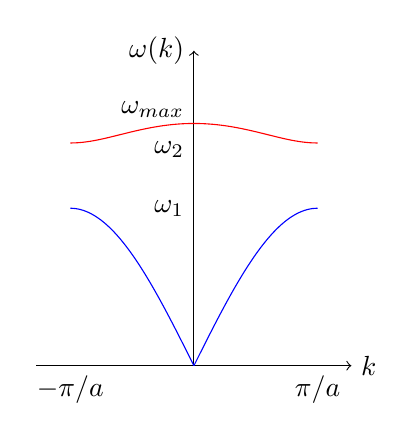
\begin{tikzpicture}
      \draw[->] (-2,0) -- (2,0) node[right] {$k$};
      \draw[->] (0,0) -- (0,4) node[left] {$\omega(k)$};
      \draw[domain=0:1.57,smooth,variable=\x,red] plot ({\x},{2*sqrt(0.5*(1+2+sqrt((1-2)^2+2*(cos(deg(\x))^2))))});
      \draw[domain=-1.57:0,smooth,variable=\x,red] plot ({\x},{2*sqrt(0.5*(1+2+sqrt((1-2)^2+2*(cos(deg(\x))^2))))});
      \draw[domain=-1.57:0,smooth,variable=\x,blue] plot ({\x},{-2*sin(deg(\x))});
      \draw[domain=0:1.57,smooth,variable=\x,blue] plot ({\x},{2*sin(deg(\x))});
      \draw (0,2) node[left]{$\omega_1$};
      \draw (0,2.75) node[left]{$\omega_2$};
      \draw (0,3.25) node[left]{$\omega_{max}$};
      \draw (1.57,0) node[below]{$\pi/a$};
      \draw (-1.57,0) node[below]{$-\pi/a$};
\end{tikzpicture}
\end{center}
The labelled $\omega$ quantities are
$$\omega_{max}=\sqrt{\frac{2\alpha(m+M)}{Mm}},\quad\omega_1=\sqrt{\frac{2\alpha}{M}},~\omega_2=\sqrt{\frac{2\alpha}{m}}$$
\end{ans}
\begin{qns}[Transport]
A monatomic free electron metal has a density of atoms of 2.5$\times10^{28}$ m$^{−3}$ and a conductivity of $2.1\times 10^7\Omega^{−1}$m$^{−1}$. Evaluate the electronic mobility and mean time between collisions for this metal.\hfill\textbf{[4]}
\end{qns}
\begin{ans}
The mobility is $\mu=\frac{\sigma}{ne}=\frac{2.1\times10^7}{2.5\times10^{28}\times 1.6\times10^{-19}}=5.25\times10^{-3}$ m$^2$ V$^{-1}$ s$^{-1}$, and the mean time between collisions is $\tau=\mu\frac{m}{e}=5.25\times10^{-3}\frac{9.11\times10^{-31}}{1.6\times10^{-19}}=3\times10^{-14}$ s.
\end{ans}
\subsubsection{Section B}
\begin{qns}[Dispersion]\leavevmode
\begin{enumerate}[label=(\roman*)]
\item Define phase velocity $u_p$ and group velocity $u_g$.\hfill\textbf{[2]}
\item Waves on deep water obey the dispersion relation for angular frequency $\omega$
$$\omega^2=gk+\frac{\sigma k^3}{\rho_1}$$
where $g$ is the gravitational acceleration, $\sigma$ and $\rho_1$ are respectively the surface tension and density of water, and $k$ is the wavenumber. Verify that the group and phase velocities are equal at one particular wavelength, $\lambda^*$, and calculate the wave speed at $\lambda^*$, for $g = 9.8$ m s$^{−2}$, $\rho_1 = 10^3$ kg m$^{−3}$ and $\sigma = 72\times 10^{-3}$ N m$^{−1}$.\hfill\textbf{[4]}
\item Find the ratio $u_g/u_p$ in the long and short wavelength limits.\hfill\textbf{[2]}
\item Consider a wavepacket which is compact at a given time. Describe or sketch the different time evolution when the wavepacket has wavelengths $>>\lambda^*$ compared with when the wavelengths are $<<\lambda^*$.\hfill\textbf{[3]}
\item If a thin elastic sheet, of thickness $a$ and density $\rho_2$ covers the water surface, the dispersion relation is modified to
$$\omega^2\bigg(1+\frac{\rho_2}{\rho_1}ak\bigg)=gk\bigg(1+\frac{\sigma k^2}{\rho_1g}+\frac{Bk^4}{\rho_1g}\bigg)$$
where $B$ is a modulus that quantifies the resistance of the sheet to bending. Take $\rho_2 = 0.8\rho_1$, $a = 10^{−4}$ m, $B = 10^{−10}$ J, and other values as above. Sketch, as a function of the wavenumber, the ratio of the frequencies observed with and without the covering sheet. Comment on the physical reasons for the behaviour of this ratio at small and large wavenumber.\hfill\textbf{[5]}
\item Assuming that this system is kept in a large container, and a square frame of edge $L = 6$ cm is lowered onto the surface pinning the boundaries, calculate by how much the lowest wave frequency allowed inside the frame is changed by the presence of the sheet.\hfill\textbf{[4]}
\end{enumerate}
\end{qns}
\begin{ans}\leavevmode
\begin{enumerate}[label=(\roman*)]
\item The phase velocity is the speed at which an individual harmonic wave with angular frequency (independent of $k$) and wavenumber $k$ travels in the system, it is given by $u_p=\frac{\omega}{k}$. The group velocity is the speed at which the interference features (such as the maximum of the profile) travels at. For a Gaussian wavepacket with central wavenumber $k$ and angular frequency $\omega(k)$, the central maximum travels at $u_g=\frac{\partial\omega}{\partial k}|_{k=k_0}$.
\item The phase velocity and group velocity of waves in deep water are respectively
$$u_p=\frac{\omega}{k}=\sqrt{\frac{g}{k}+\frac{\sigma k}{\rho_1}}$$
$$2\frac{\omega}{k}\frac{\partial\omega}{\partial k}=\frac{g}{k}+\frac{3\sigma k}{\rho_1}\implies u_g=\frac{\frac{g}{k}+\frac{3\sigma k}{\rho_1}}{2\sqrt{\frac{g}{k}+\frac{\sigma k}{\rho_1}}}$$
For $u_p=u_g$ at wavelength $\lambda=\lambda^*$, then
$$\frac{\frac{2g}{k}+\frac{2\sigma k}{\rho_1}}{\frac{g}{k}+\frac{3\sigma k}{\rho_1}}=1\implies\frac{g}{k}=\frac{\sigma k}{\rho_1}\implies\lambda^*=2\pi\sqrt{\frac{\sigma}{g\rho_1}}=2\pi\sqrt{\frac{72\times10^{-3}}{9.8\times10^3}}=0.017m$$
\item For short wavelengths, $\frac{1}{k}<<1$:
$$\frac{u_g}{u_p}=\frac{\rho_1}{2\sigma}\bigg(\frac{3\sigma}{\rho_1}+\frac{g}{k^2}\bigg)\bigg(1+\frac{g\rho_1}{\sigma k^2}\bigg)^{-1}\approx\frac{\rho_1}{2\sigma}\bigg(\frac{3\sigma}{\rho_1}+\frac{g}{k^2}\bigg)\bigg(1-\frac{g\rho_1}{\sigma k^2}\bigg)\approx\frac{3}{2}$$
For long wavelengths, $k<<1$:
$$\frac{u_g}{u_p}=\frac{1}{2g}\bigg(g+\frac{3\sigma k^2}{\rho_1}\bigg)\bigg(1+\frac{\sigma k^2}{\rho_1g}\bigg)^{-1}\approx\frac{1}{2g}\bigg(g+\frac{3\sigma k^2}{\rho_1}\bigg)\bigg(1-\frac{\sigma k^2}{\rho_1g}\bigg)\approx\frac{1}{2}$$
\item For wavelengths $>>\lambda^*$, we are in the long wavelength limit and so $u_g=\frac{1}{2}u_p<u_p$, resulting in wave to accumulate at the front, i.e. positive dispersion. On the other hand, for wavelengths $<<\lambda^*$, we are in the short wavelength limit and so $u_g=\frac{3}{2}u_p>u_p$, resulting in waves to pile up at the back, i.e. negative dispersion.
\item Let $\omega_0^2=gk+\frac{\sigma k^3}{\rho_1}$, then the ratio of $\omega^2$ to $\omega_0^2$ is
$$\frac{\omega^2}{\omega_0^2}=\frac{gk(1+\frac{\sigma k^2}{\rho_1g}+\frac{Bk^4}{\rho_1g})}{(1+\frac{\rho_2}{\rho_1}ak)gk(1+\frac{\sigma k^2}{g\rho_1})}$$
We have $\lim_{k\rightarrow0}\frac{\omega^2}{\omega_0^2}\approx(1+\frac{\sigma k^2}{\rho_1g}(1-\frac{\rho_2}{\rho_1}ak)\approx 1$ and $\lim_{k\rightarrow\infty}\frac{\omega^2}{\omega_0^2}\approx\frac{Bkg\rho_1^2}{\rho_1g\rho_2\sigma a}\rightarrow\infty$.
\item $\lambda_0=2\times L=0.12$ m, while $k=\sqrt{(2\pi/2L)^2+(2\pi/2L)^2}=\sqrt{2}\frac{\pi}{L}$. 
$$\omega_0^2(\lambda_0)=g\sqrt{2}\frac{\pi}{L}+\frac{2\sqrt{2}\sigma\pi^3}{\rho_1L}=\frac{\sqrt{2}\pi9.8}{0.06}+\frac{2\sqrt{2}(72\times10^{-3})}{0.06^3(10^3)}\pi^3\implies\omega_0=27.4755$$
$$\omega^2(\lambda_0)=\frac{g\sqrt{2}\frac{\pi}{L}(1+\frac{\sigma}{\rho_1g}\frac{2\pi^2}{L^2}+\frac{B}{\rho_1g}\frac{4\pi^4}{L^4})}{1+\frac{\rho_2}{\rho_1}a\sqrt{2}\frac{\pi}{L}}=\frac{9.8\sqrt{2}\frac{\pi}{0.06}(1+\frac{72\times10^{-3}}{9.8(10^3)}\frac{2\pi^2}{0.06^2}+\frac{10^{-10}}{9.8(10^3)}\frac{4\pi^4}{0.06^4})}{1+0.8(10^{-4})\sqrt{2}\frac{\pi}{0.06}}\implies\omega=27.3945$$
The lowest frequency have changed by $\frac{\omega-\omega_0}{2\pi}=-0.0129$ Hz.
\end{enumerate}
\end{ans}
\newpage
\begin{qns}[Fabry-Pérot]
A Fabry–Pérot interferometer consists of two flat glass plates separated by a distance $d$. The two inner surfaces are coated and have intensity reflection coefficient $R$; $\mu$ and $\mu_0$ are the refractive indices of the medium between and outside the plates respectively.
If an extended monochromatic source of light is observed through the interferometer, light is incident over a range of angles. The subsequent paths of one incident ray are shown in the figure.
\begin{figure}[H]
    \centering
    \includegraphics[scale=0.5]{2012P2B7Q.PNG}
\end{figure}
\begin{enumerate}[label=(\roman*)]
\item Calculate the phase difference $\delta$ between the adjacent rays that exit the cavity as shown in the figure, and thus show that sharp bright rings are observed in the far-field when $2k_0\mu d\cos\theta=2m\pi$, where $m$ is an integer, $k_0$ is the wavenumber of the light in vacuum and $\theta$ is as labelled in the figure.\hfill\textbf{[4]}
\item Show that, for a fixed angle $\theta$, the transmittance (the emitted fraction of the incident intensity) is given by\hfill\textbf{[6]}
$$T_e=\frac{(1-R)^2}{1+R^2-2R\cos\delta}$$
\item The interferometer is now illuminated by a broadband source. Show that for a fixed angle $\theta$, adjacent transmission peaks occur at a wavelength separation (called the free spectral range) given approximately by
$$\Delta\lambda\approx\frac{\lambda_0^2}{2\mu d\cos\theta}$$
where $\lambda_0$ is the central wavelength of the nearest transmission peak.\hfill\textbf{[2]}\\[5pt]
A quantity, $\mathcal{F}$, known as the finesse of the interferometer is defined as $\mathcal{F}=\frac{\Delta\lambda}{\delta\lambda}$, where $\delta\lambda$ is the full-width half-maximum of the transmission for a particular order. It can be shown that the finesse is approximately
$$\mathcal{F}=\frac{\pi R^{1/2}}{1-R}$$
\item A Fabry–Pérot interferometer is used to measure a spectrum that consists of two lines centred at $\lambda_1 = 670$ nm, with separation $\Delta\lambda_1=1$ nm, and another line at $\lambda_2=$ 633 nm. Derive appropriate values of $d$ and $R$ for measuring this spectrum, when observations are made varying $\theta$.\hfill\textbf{[5]}
\item Discuss why a Fabry–Pérot interferometer can have a much higher resolving power than a Michelson interferometer of similar physical dimensions, and what the requirements on the flatness of the surfaces are, in order to achieve this higher theoretical resolving power.\hfill\textbf{[3]}
\end{enumerate}
\end{qns}
\begin{ans}\leavevmode
\begin{enumerate}[label=(\roman*)]
\item Consider an event of beam splitting. The two beams travel until they emerge into the air. The second beam will travel an additional distance $L=2d\sec\theta$ in the medium of refractive index $\mu$, then the two beams both travel the same distance in the glass. The first beam travels an extra distance $l=2x\sin\beta$ in air. After this, the two beams travel parallel to the distant observer. Snell's law gives $\frac{\sin\theta}{\sin\alpha}=\frac{\mu_0}{\mu}$ and $\frac{\sin\alpha}{\sin\beta}=\frac{1}{\mu_0}$, which gives $\sin\beta=\mu\sin\theta$. As the wavenumber in the medium $\mu(k)$ is related to the wavenumber in air $k_0$, then we have $k=\mu k_0$. The phase difference is 
$$\delta =kL-k_0l=\mu_0k_02d\sec\theta-k_02d\tan\theta\mu\sin\theta=2d\mu k_0\bigg(\frac{1}{\cos\theta}-\frac{\sin^2\theta}{\cos\theta}\bigg)=2d\mu k_0\cos\theta$$
For consecutive interference, $\delta=2k_0\mu d\cos\theta=2m\pi$, for $m\in\mathbb{Z}$. These will appear as circles if we are far away from the normal of the glass.
\item The $n$th beam will have been transmitted twice (once in and once out) and reflected $2(n-1)$ times, and accrued a relative phase difference of $(n-1)\delta$, giving us an amplitude
$$A=A_0(1-R)+A_0(1-R)e^{o\delta}+A_0(1-R)R^2e^{2i\delta}+...=A_0(1-R)\sum_{n=0}^\infty (Re^{i\delta})^n=\frac{A_0(1-R)}{1-Re^{i\delta}}$$
The ratio of outgoing intensity to the incident intensity gives the transmittance.
$$T_e=\frac{I}{I_0}=\frac{(1-R)^2}{(1-Re^{i\delta})(1-Re^{-i\delta})}=\frac{(1-R)^2}{1+R^2-2R\cos\delta}$$
\item For the $m$th order peak corresponding to wavelength $\lambda$, $2\frac{2\pi}{\lambda}\mu d\cos\theta=2m\pi$, so if $\theta$ corresponds to $m$th peak of $\lambda_0$, and also $(m-1)$th peak of $\lambda_0+\Delta\lambda$, 
$$2\mu d\cos\theta=m\lambda_0=(m-1)(\lambda_0+\Delta\lambda)\implies m=\frac{\lambda_0}{\Delta\lambda}+1$$
We then have $2\mu d\cos\theta=\frac{\lambda_0^2}{\Delta\lambda}+\lambda_0\implies\Delta\lambda\approx\frac{\lambda_0^2}{2\mu d\cos\theta}$ for $\frac{\lambda_0}{\Delta\lambda}>>1$.
\item The separation $d$ is determined by the requirement that we can resolve the peaks that are farthest apart in wavelength, as we do not want the orders to overlap. $\mu d\cos\theta\sim\frac{\lambda_0^2}{2\mu\Delta\lambda}\sim 6\mu$m, and so we are looking at an order $m\sim 9$. To find $\delta\lambda$, we need the full width half maximum of $T_e$:
$$\frac{1}{2}\frac{(1-R)^2}{1+R^2-2R}=\frac{(1-R)^2}{1+R^2-2R\cos\delta}\implies (1-R)^2=2R(1-\cos\delta)$$
where $\delta$ is the phase of the $m$th order of the line of $\lambda_0+\delta\lambda=633$ nm relative to that corresponding to the $m$th order maximum of the line at $\lambda_0=632$ nm. Hence,
$$2\mu k_0\cos\theta=2m\pi\implies\delta=2\mu k\cos\theta=2m\pi\frac{\lambda_0}{\lambda}\implies\cos\delta\sim 0.3$$
which gives $R^2-1+2R(1-0.3)=0\implies R=0.5$.
\item In practice, we cannot sum the geometric series in $A$ to infinity, given the finite extent of the etalon. The resultant finite total path difference will blur the resolution.\\[5pt]
There are problems even if we use the Fabry-Pérot at normal configuration ($\theta=0$ and vary $d$). The plates cannot be perfectly flat when the plates are moved. Any slight misalignment will lead to an extra path difference, of value $m$ times this misalignment.\\[5pt]
In comparison, for a Michelson interferometer, the path difference is generated by only one reflection. As a result, the physical dimensions of the setup need to be larger by a factor of order $m$, in order to achieve the same resolution as the etalon. Moreover, the Michelson interferometer faces the same issue of finite optical path length available.
\end{enumerate}
\end{ans}
\newpage
\begin{qns}[Fraunhofer Diffraction]\leavevmode
\begin{enumerate}[label=(\roman*)]
\item State the conditions for Fraunhofer diffraction to apply, and how it can be achieved in practice.\hfill\textbf{[2]}
\item Explain why the complex amplitude $\phi$ is given by the Fraunhofer integral
$$\phi\propto\int\int_{\Sigma}\phi_{\Sigma}\exp\bigg[-ik\bigg(\frac{x_0x+y_0y}{R}\bigg)\bigg]dxdy$$
defining the quantities in this relation with a labelled sketch.\hfill\textbf{[4]}
\item Show, for the particular case of one-dimensional slits, that the aperture function can be recovered from a Fourier transform of the Fraunhofer diffracted field. \hfill\textbf{[4]}\\[5pt]
An interferometric radio telescope is made of 10 dishes whose centres are separated by $D =$ 800 m, aligned East–West on the equator, pointing directly overhead. Each dish has diameter 25 m. The interferometer operates at $\lambda =$ 6 cm.
\item Consider first the dishes as synchronised emitters. Approximately how far away does an observer need to be in order to measure the Fraunhofer diffraction pattern? Show that in this case the intensity pattern observed as a function of angle is given approximately by:
$$I(\theta)=I\bigg[\frac{\sin(10k_0\frac{D}{2}\theta)}{\sin(k_0\frac{D}{2}\theta)}\bigg]^2$$
where $\theta$ is measured from the vertical, and $k_0=\frac{2\pi}{\lambda}$. State any assumptions made regarding the effect of the dish diameters.\hfill\textbf{[4]}
\item Sketch and label this intensity pattern.\hfill\textbf{[3]}
\item Now the same radio telescope is used in reception mode. Due to the Earth’s rotation a bright source in the sky appears to move relative to the telescope. Through what angle must the source move to pass from the zero order maximum to the first minimum?\hfill\textbf{[3]}
\end{enumerate}
\end{qns}
\begin{ans}\leavevmode
\begin{enumerate}[label=(\roman*)]
\item In the Fraunhofer regime, the phase variation as seen from any given point on the aperture plane is linear in the distance in the aperture. Place the source and the screen at conjugate points of the two lenses located on the left and right side of the aperture plane.
\item Focusing on the linear phase variation, the Fresnel-Kirchoff diffraction integral can be approximated as
$$\phi\propto\int\int_\Sigma\psi_\Sigma e^{-ik\frac{x_0x+y_0y}{R}}dxdy$$
where $k$ is the wavenumber of the light used, $\psi_\Sigma$ is the incident amplitude on the aperture plane $\Sigma$, $r$ is the distance from the aperture point on the plane $(x_0,y_0)$ to the point on the screen $(x,y)$, where $r$ is
$$r=\sqrt{(x-x_0)^2+(y-y_0)^2+L^2}\approx R\bigg(1-\frac{2(xx_0+yy_0)}{2R^2}\bigg)$$
where $R^2=x_0^2+y_0^2+L^2$, $R>>x,x_0,y,y_0$, and that the higher order terms in the approximation have been dropped.
\item Take $y=0$ since one-dimensional. Assuming small angle approximation holds, i.e. $\sin\theta\approx\tan\theta=\frac{x_0}{R}$, then
$$\phi\propto\int_\Sigma\psi_\Sigma e^{-ik\sin\theta}dx\propto\int_{\mathbb{R}}h(x)e^{-ik\sin\theta}dx$$
where the complex amplitude is akin to a Fourier transform of the aperture function $h(x)$. The result is a function of the Fourier conjugate variable, $k\sin\theta$.
\item The setup is akin to a 10-slit diffraction grating with $N=10$, $D=800$ m, $a=25$ m, $\lambda=6\times10^{-2}$ m. We have $\frac{a^2}{\lambda}=\frac{25^2}{6\times10^{-2}}=10417$. In order to measure Fraunhofer diffraction pattern, the observer must stand much farther than 10 km. Observe that $\frac{a}{D}=\frac{25}{800}=\frac{1}{32}<<1$, and so we argue that the width of the slit is negligible compared to the spacing of the slit. The aperture function is
$$h(x)=\sum_{n=0}^9\delta(x-nD)\implies\phi\propto\int h(x)e^{-ik\sin\theta}dx=e^{-ik\sin\theta(9/2)D}\frac{\sin(10k\sin\theta D/2)}{\sin(k\sin\theta D/2)}$$
The intensity is proportional to the modulus of the complex amplitude, and taking $k=k_0$, $\sin\theta\approx\theta$, we obtain our desired result.
\item The intensity plot is
\pgfplotsset{ticks=none}
\begin{center}
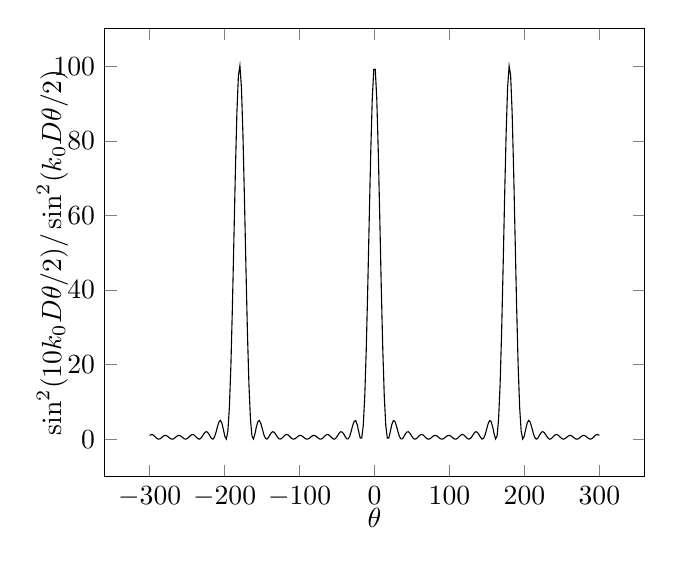
\begin{tikzpicture} 
    \begin{axis}[
    x label style={at={(axis description cs:0.5,-0.05)},anchor=north},
    y label style={at={(axis description cs:-0.05,.5)},anchor=south},
    ylabel={$\sin^2(10k_0D\theta/2)/\sin^2(k_0D\theta/2)$},
    xlabel={$\theta$}]
      \addplot [domain = -300:300, samples = 300] ({\x},{(sin(10*\x)/sin(\x))^2});
 \end{axis}
\end{tikzpicture}
\end{center}
\item The first zero of the $\sinc$ curve occurs at $k_0D\theta=\frac{2\pi}{N}\implies\theta=\frac{\lambda}{DN}=\frac{6\times10^{-2}}{800\times 10}=7.5\times10^{-6}$ radians.
\end{enumerate}
\end{ans}
\newpage
\begin{qns}[Impedance]\leavevmode
\begin{enumerate}[label=(\roman*)]
\item Consider a string of mass per unit length $\rho$ held under a tension $T$. Explain what is meant by the characteristic impedance $Z$ of the string, and how it depends on $T$ and $\rho$. Evaluate the mean power transmitted by a travelling wave in terms of $Z$, $\omega$ and its amplitude $A$.\hfill\textbf{[4]}\\[5pt]
Two long pieces of string of mass per unit length $\rho_0$ and $4\rho_0$ are connected together as shown in the figure, and held under a tension $T$, assumed to be constant.
\begin{figure}[H]
    \centering
    \includegraphics[scale=0.75]{2012P2B9Q.PNG}
\end{figure}
\item Consider a sinusoidal transverse wave of the form
$$\psi=\text{Re}(\psi_0e^{i(kx-\omega t)})$$
propagating in the lighter string in the $x$-direction, giving rise to reflected and transmitted waves. Obtain an expression for the disturbance which is set up in the light string, showing that it can be written as a sum of a standing wave and a travelling wave.\hfill\textbf{[5]}
\item Find the reflection and transmission coefficients, and the standing wave ratio (the ratio of maximum to minimum amplitude of oscillation) in the light string.\hfill\textbf{[3]}
\item An additional piece of string is inserted in between the two long pieces considered above. This new segment of string has different density and is of length $a$. Without detailed calculations, explain under what conditions, if any, it is possible to transmit fully the incident wave coming from the light string.\hfill\textbf{[5]}
\item A different piece of string is inserted between the two original strings. This new segment of string has density varying gradually from $\rho_0$ to $4\rho_0$, and has a length which is much greater than the incident wavelength. Under these conditions there is no reflection. What are the frequency, amplitude and wavelength of the wave in the heavier string, relative to the incident wave values?\hfill\textbf{[3]}
\end{enumerate}
\end{qns}
\begin{ans}\leavevmode
\begin{enumerate}[label=(\roman*)]
\item The characteristic impedance is defined for a harmonic wave $\psi=\text{Re}[Ae^{i(kx-\omega t)}]$ and it is the ratio of the complex driving force to the complex velocity response by
$$Z=-\frac{T\psi'}{\dot{\psi}}=T\frac{-ik\psi}{-i\omega\psi}=\frac{T}{v_p}$$
where $v_p$ is the phase velocity and $v_p=\sqrt{T/\rho}$ from the wave equation. Hence, $Z=\sqrt{T\rho}$.\\[5pt]
The instantaneous power of a harmonic travelling wave is 
$$P=\text{Re}[F]\text{Re}[v]=\frac{1}{2}(F+F^*)(v+v^*)=\frac{1}{4}(Fv+(Fv)^*+Fv^*+(Fv^*)^*)$$
which is basically $\frac{1}{2}\text{Re}[Fv]+\frac{1}{2}\text{Re}[Fv^*]=\frac{1}{2}\text{Re}[F_0v_0e^{2i\omega t}]+\frac{1}{2}\text{Re}[F_0v_0]$. Taking the time-averaged of the power, the first term is zero due to $\langle\cos2\omega t\rangle=0$ while the second term is non-zero. So, $\langle P\rangle=\frac{1}{2}\text{Re}[Zvv^*]=\frac{1}{2}|A|^2\omega^2\text{Re}[Z]$.
\item In the two regions, we guess
$$\psi(x,t)=
\left\{
        \begin{array}{ll}
      \text{Re}[\psi_0e^{i(kx-\omega t)}+r\psi_0e^{i(-kx-i\omega t)} & x<0\\
      \text{Re}[\tau\psi_0e^{i(qx-\Omega t)}] & x>0
        \end{array}
    \right.$$
where $r$ and $\tau$ are the reflection and transmission amplitude coefficients respectively, $q$ and $\Omega$ are the angular frequency and wavenumber respectively in $x>0$. The wave in $x<0$ can be written as
$$\psi=\text{Re}[\psi_0e^{-i\omega t}(e^{ikx}+re^{-ikx})]=(1-r)|\psi_0|\cos(kx-\omega t+\text{arg}(\psi_0))+(1+r)|\psi_0|\cos(\arg(\psi_0)-\omega t)\cos(2kx)$$
The first term is a travelling wave, while the second term is a standing wave. 
\item  $\psi$ and $\psi'$ continuous $\forall x$ and $\forall t$. So, for convenience, set $x=0$. Then,
$$e^{-i\omega t}+re^{-i\omega t}=\tau e^{-i\Omega t}$$
$$ik(e^{-i\omega t}-re^{-i\omega t})=iqe^{-i\Omega t}$$
For this to be true $\forall t$, we have $\omega=\Omega$, $$1+r=\tau,\quad 1-r=\tau\frac{q}{k}$$ 
But, $\frac{q}{k}=\frac{q}{\omega}\frac{\omega}{k}=\frac{v_1}{v_2}=\frac{Z_2}{Z_1}$. Rearranging gives $r=\frac{1-(Z_2/Z_1)}{1+(Z_2/Z_1)}$. But since we have $\rho_0$ and $4\rho_0$, the reflection coefficient is $\frac{1-\sqrt{4}}{1+\sqrt{4}}=-\frac{1}{3}$. 
$$\psi=\text{Re}[\psi_0e^{-i\omega t}(e^{ikx}-\frac{1}{3}e^{-ikx})]=\frac{4}{3}|\psi_0|\cos(kx-\omega t+\text{arg}(\psi_0))-\frac{2}{3}|\psi_0|\cos(\arg(\psi_0)-\omega t)\cos(2kx)$$
The standing wave ratio (SWR) is a ratio of the instantaneous amplitude at $x=0$ and $t=\frac{\arg(\psi_0)}{\omega}$ to that at $2kx=\frac{\pi}{2}$ and when $kx-\omega t+\arg(\psi_0)$. Hence, SWR is 
$$\frac{4/3-2/3}{4/3}=\frac{1}{2}$$
while the transmission coefficient is $\tau=1+r=\frac{2}{3}$.
\item For no reflection, we must choose the impedance of the intermediate region $Z_3$ to be the geometric mean of $Z_1$ and $Z_2$, and choose the value of $a$ such that in this region, $a=\frac{\lambda}{4}(1+4n)$.
\item For this new configuration, same frequencies in each region, the ratio of wavelengths is $\frac{\lambda_2}{\lambda_1}=\frac{Z_1}{Z_2}=\frac{1}{2}$. Since the powers are equal, the ratio of amplitude is $\frac{|A_1|}{|A_2|}=\sqrt{\frac{Z_2}{Z_1}}=\sqrt{2}$.
\end{enumerate}
\end{ans}
\newpage
\subsubsection{Section C}
\begin{qns}[Band Structure]\leavevmode
\begin{enumerate}[label=(\roman*)]
\item Discuss, without mathematical detail, the origin of the band gap in semiconductors.\hfill\textbf{[8]}
\item In a particular direct gap semiconductor, the top of the valence band and the bottom of the conduction band are both located at the wavevector $k = 0$. The band gap $E_g$ is 0.18 eV, the effective mass of an electron in the conduction band is $m_e^*=0.14 m_e$, and the effective mass of a hole in the valence band is $m_h^*=0.4 m_e$, where $m_e$ is the free electron mass. A photon of energy 0.5 eV excites an electron from the valence to the conduction band. Sketch the energy bands and, on the assumption that a phonon is not involved and the wave vector of the photon is much less than the Fermi wavevector, show the electronic transition which occurs.\hfill\textbf{[2]}
\item Evaluate the initial and final energies of the electron, taking the zero of energy to be at the top of the valence band.\hfill\textbf{[4]}
\item If impurities are introduced into the semiconductor, new energy levels are introduced into the gap. Sketch their position for the introduction of n- and p-type impurities respectively, and briefly explain why they sit where they do.\hfill\textbf{[4]}
\item If the effective mass of the electron associated with a trivalent impurity is $0.1 m_e$, and the dielectric constant of the material is 12, evaluate the ionisation potential of the singly-ionised impurity, commenting on this result.\hfill\textbf{[2]}
\end{enumerate}
\begin{mdframed}
\color{darkblue}{The energy levels of the Hydrogen atom are given by$$E_n=-\frac{me^4}{2\hbar^2n^2(4\pi\epsilon_0)^2}=-\frac{1}{n^2}13.6eV$$
}
\end{mdframed}
\end{qns}
\begin{ans}\leavevmode
\begin{enumerate}[label=(\roman*)]
\item The free electron model assumes the occupied electron states are either extremely localized `bonding' electrons or delocalized states. The latter interact with the atomic nuclei and the former through an assumed constant mean field. The solutions to this system are plane waves with a dispersion relation of $E=p^2/2m_e$ for non-relativistic electrons.\\[5pt]
The nearly free electron model refines this approach by considering the background potential as a constant potential plus a small perturbation $\Delta H$. Due to the translational symmetry of the lattice, this potential will be Fourier expandable as
$$\Delta H=\sum_{h,k,l}V_p\cos(\mathbf{G_{hkl}}\cdot\mathbf{x})$$
where $\mathbf{G_{hkl}}$ is a reciprocal lattice vector. With this perturbation, the previous eigenstates $|\phi_n\rangle$ will be hybridized by
$$|\phi_n\rangle\rightarrow|\phi_n\rangle+\sum_{m\neq n}c_{nm}|\phi_m\rangle$$
with the coefficients $c_{nm}$ given by the first order time-independent perturbation (from Part II) as
$$c_{mn}=\frac{\langle\phi_n|\Delta H|\phi_m\rangle}{E_m-E_n}$$
and so there will only be significant hybridization between states of similar energies and states that are an integer number of reciprocal lattice vectors apart. This means that deviations from the quadratic dispersion relation will only be seen at the Brillouin Zone boundaries and at the centre.\\[5pt]
Since electrons are fermions, each state can only be occupied by a finite number of electrons (two for each quantum state of the same energy since electrons have spin-half). For certain materials, it is possible that at temperture $T$, all the occupied states are separated from the next available state
\begin{itemize}
    \item by an infinitesimal energy gap: conductors
    \item by a large energy gap (comparable to $k_BT$): insulators
    \item by a moderate energy gap ($\sim k_BT$): semi-conductors
\end{itemize}
\item Since the momentum of the photon is much smaller than the momenta of the starting or ending phonons (for photons $E=|\mathbf{p}|c$ while for phonons $E\sim|\mathbf{p}|v_s$ where $v_s<<c$ is the speed of the sound in the material). This makes the transition practically vertical. Since the bandgap is less than the energy of the transition, it must occur off-centre, i.e. involve a phonon.
\item Model the conduction and valence bands as quadratic, with the initial and final energies of the electron to be
$$\hbar\omega_u=E_g+\frac{1}{2}\frac{\hbar^2}{0.14m_e}k^2$$
$$\hbar\omega_l=-\frac{1}{2}\frac{\hbar^2}{0.4m_e}k^2$$
The bandgap is given as $E_g=0.18$eV and the change in energy of the electron is $E_0=0.5$eV:
$$0.5=E_0=0.18+\frac{\hbar^2k^2}{2m_e}\bigg(\frac{1}{0.14}-\frac{-1}{0.4}\bigg)\implies\frac{\hbar^2k^2}{2m_e}=33.2meV$$
Hence, the initial and final energies are $\hbar\omega_l=(33.2/-0.4)=-83$ meV and $\hbar\omega_u=(33.2/0.14)=0.237$ eV.
\item The new energy states are highly localized in real space, and hence delocalized in $k$-space. Thus, they are represented as horizontal lines (no $k$-dependence). Since the ionization energies of the impurities (electrons and holes respectively) are very much than the bandgap $E_g$, the energies are quite close to the conduction/valence bands. 
\item The ionization energy is
$$\frac{m^*}{m_e}\frac{1}{\epsilon^2}13.6=\frac{13.6(0.1)}{12^2}=9.4meV$$
Hence, the p-donor levels are very close to the valence band. At room temperature, $k_BT=(1.38\times10^{-23})(300)=26$ meV, greater than the ionization energy, hence all p-donor states are excited.
\end{enumerate}
\end{ans}
\begin{qns}[Heat Capacity]\leavevmode
\begin{enumerate}[label=(\roman*)]
\item Working within the free electron model, derive expressions for the Fermi energy $E_F$ and the density of states $g(E_F)$.\hfill\textbf{[6]}
\item Hence evaluate the density of states at the Fermi energy for magnesium, which has a valence of two and an atomic concentration of $4.3\times 10^{28}$ m$^{−3}$.\hfill\textbf{[4]}
\item Using this value of $g(E_F)$, estimate the electronic contribution to the heat capacity of magnesium.\hfill\textbf{[4]}
\item Sketch the general form of the heat capacity of a metal as a function of temperature, briefly explaining the different regimes of behaviour (detailed mathematics is not required).\hfill\textbf{[4]}
\item Outline why the electronic contribution to the heat capacity of a metal is negligible at room temperature.\hfill\textbf{[2]}
\end{enumerate}
\end{qns}
\newpage
\begin{ans}\leavevmode
\begin{enumerate}[label=(\roman*)]
\item In the Free Electron Model, each lattice point contributes $n$ delocalized electrons, where $n$ is known as the valency. The delocalized electrons occupy plane wave states, and because each electron is a spin-half fermion, each electron can only occupy a single state. The Fermi energy $E_F$ is defined to be the energy of the highest occupied state. To get the density of states $g(E_F)$, we take a crystal of linear size $L$ and impose periodic boundary conditions, thus giving us $L=n\lambda\implies p=\frac{h}{\lambda}=\frac{nh}{L}$, so each state in $p$-space occupies a cube of size $(h/L)^3$. The number of states available for a particle with momentum in the range $[p,p+dp]$ is
$$g(p)dp=2(4\pi p^2dp)\frac{1}{(h/L)^3}=\frac{8\pi V}{h^3}p^2dp$$
where 2 is the spin degeneracy factor, $4\pi p^2dp$ is the corresponding differential volume in $p$-space and $V=L^3$ is the volume of the crystal. Assuming the electrons are non-relativistic, $E=\frac{p^2}{2m}\implies mdE=pdp$, so
$$g(E)dE=\frac{8\sqrt{2}\pi Vm^{3/2}}{h^3}\sqrt{E}dE$$
but the total number of states occupied is fixed at $N$, with the Fermi energy $E_F$ being the highest energy
$$N=\int_0^{E_F}g(E)dE=\frac{V8\sqrt{2}\pi m^{3/2}}{h^3}\int_0^{E_F}\sqrt{E}dE=\frac{16\sqrt{2}V\pi m^{3/2}}{3h^3}E_F^{3/2}$$
so the Fermi energy and the corresponding density of states is
$$E_F=\frac{h^2}{2m}\bigg(\frac{3N}{8\pi V}\bigg)^{2/3},\quad g(E_F)=\frac{8\pi Vm}{h^2}\bigg(\frac{N}{V}\frac{3}{8\pi}\bigg)^{1/3}$$
\item We are given $E_F=6.9$ eV and the electron concentration be $\frac{N}{V}=2\times(4.3\times10^{28})$ m$^{-3}$ where Magnesium has a valency of 2, so the density of states per unit volume is
$$\frac{8\sqrt{2}\pi m^{3/2}}{h^3}E_F^{1/2}=\frac{8\sqrt{2}\pi\sqrt{6.9(1.6\times10^{-19})}}{(6.626\times10^{-34})^3}(9.11\times10^{-31})^{3/2}=1.12\times10^{47}m^{-3}J^{-1}$$
\item Since only electrons of energy within $k_BT$ of the Fermi energy can be excited (due to the fact that deeper electrons not having empty states available). The thermal energy per unit volume is thus
$$U_{th}\sim\frac{3}{2}k_BTg(E_F)k_BT\sim \frac{3}{2}k_B^2T^2g(E_F)$$
where $\frac{3}{2}k_BT$ is the energy per state and so the corresponding heat capacity is
$$C_V\sim\frac{\partial U_{th}}{\partial T}=3k_B^2Tg(E_F)=3(1.38\times10^{-23})^2(300)(1.1\times10^{47})=1.89\times10^4Jkg^{-1}K^{-1}$$
\item At high temperatures, the phononic heat capacity approximately plateaus to $3k_B$ per atom as all the phonon modes are activated (all 6 degrees of freedom). This dominates over the electronic contribution as the temperature at which all the electrons can be excited is way above the melting point. At low temperatures, the cubic phononic contribution will be smaller than the linear electronic contribution.
\item At temperature ranges where the metal remains a solid, the number of electrons available for thermal excitation is much less than that of phonons.

\end{enumerate}
\end{ans}
\newpage
\subsubsection{Section D}
\begin{qns}[OWO Essay]
Write an essay on the $Q$ factor in different damping regimes, with physical examples.\hfill\textbf{[20]}
\end{qns}
\begin{ans}
Quality factor is defined to be the number of cycles for the amplitude to decrease by a factor of $e^{-\pi}$. To complete $Q$ number of cycles, the time taken can be obtained from $\omega_ut=2\pi Q$. We write $Q$ as a ratio, i.e.
$$Q=\frac{\omega_0}{\gamma}$$
We study the problem on damped oscillation by considering a freely oscillating system subjected to a linear friction term (proportional to velocity), then our equation of motion will be
$$-kx-b\dot{x}=m\ddot{x}$$
which can be rewritten in the following form:
$$\ddot{x}+\gamma\dot{x}+\omega_0^2x=0$$
which is a second order, linear homogeneous differential equation, where we took $\gamma=b/m$ and $\omega_0^2=k/m$. The solutions for a damped oscillating system
$$\ddot{x}+\gamma\dot{x}+\omega_0^2x=0$$
are as follows:
\begin{enumerate}
    \item $x(t)=e^{-0.5\gamma t}[C_1e^{i\omega_ut}+C_2e^{-i\omega_ut}]$, where $\omega_u=\omega_0\sqrt{1-0.25(\gamma/\omega_0)^2}<\omega_0$.
    \item $x(t)=C_3e^{-\mu_1t}+C_4e^{-\mu_2t}$ where $\mu_{1,2}=0.5\gamma\pm\sqrt{-\omega_0^2+0.25\gamma^2}$.
    \item $x(t)=(C_5+C_6t)e^{-0.5\gamma t}$.
\end{enumerate}
where $C_1$, $C_2$, $C_3$, $C_4$ and $C_5$ are arbitrary constants that are dependent on boundary conditions. This is illustrated below: red, black blue respectively.
\begin{center}
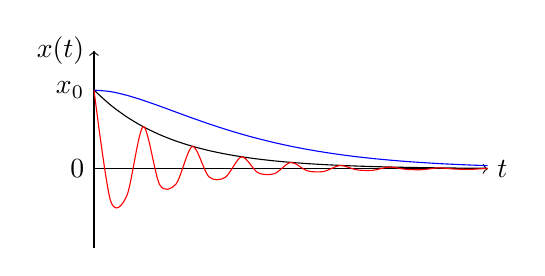
\begin{tikzpicture}
      \draw[->] (0,0) -- (5,0) node[right] {$t$};
      \draw[->] (0,-1) -- (0,1.5) node[left] {$x(t)$};
      \draw[domain=0:5,smooth,variable=\x,black] plot ({\x},{exp(-\x)});
      \draw[domain=0:5,smooth,variable=\x,blue] plot ({\x},{(1+\x)*exp(-\x)});
      \draw[domain=0:5,smooth,variable=\x,red] plot ({\x},{exp(-\x)*cos(10*\x*180/pi)});
      \draw (0,0) node[left]{0};
    \draw (0,1) node[left]{$x_0$};
\end{tikzpicture}
\end{center}
Suppose $\gamma<2\omega_0$, such that the damping is small, then the oscillation is said to be underdamped. The general solution for an underdamped solution is
$$x(t)=e^{-0.5\gamma t}(c_1\cos(\omega_ut)+c_2\sin(\omega_ut))$$
where $\omega_u=\sqrt{\omega_0^2-0.25\gamma^2}$ and the constants $c_1$ and $c_2$ are dependent on the initial conditions. If the initial conditions are $x(t=0)=x_0$ and $\dot{x}(t=0)=v_0$, then the solution is
$$x(t)=e^{-0.5\gamma t}\bigg(x_0\cos(\omega_ut)+\frac{v_0+0.5\gamma x_0}{\omega_u}\sin(\omega_ut)\bigg)$$
which is an oscillatory solution with a decaying envelope. The mean loss of energy is the time average power dissipated by the friction, i.e. $-b\langle\dot{x}^2\rangle$. One example of light damping is a pendulum freely oscillating in air with air resistance. For very light damping, $\omega_u\approx\omega_0$ and one can approximate this as $\frac{2\pi Q}{\omega_0}=\frac{2\pi}{\gamma}$ such that $e^{-0.5\gamma t}=e^{-0.5\gamma(2\pi/\gamma)}=e^{-\pi}$. Since the condition for light damping is $\gamma<2\omega_0$, $Q>0.5$. The greater the quality factor, the smaller the damping.\\[5pt]
We could also have considered the ratio of amplitude of the $(n+1)$th peak to that of the $n$th peak, bearing in mind that the amplitudes are related by the exponential term $e^{-0.5\gamma t}$:
$$\frac{a_{n+1}}{a_n}=e^{-\gamma(t_{n+1}-t_n)}$$
The time difference between the $n$th peak and the $(n+1)$th peak is related to the period of the under-damped oscillation which is $\frac{2\pi}{\omega_u}$. We denote the quantity $\Delta$ to be the logarithmic decrement $\ln(a_{n+1}/a_n)$:
$$\Delta=\ln(e^{-\frac{1}{2}\frac{2\pi\gamma}{\omega_u}})=-\frac{\pi\gamma}{\omega_u}\approx-\frac{\pi\gamma}{\omega_0}=-\frac{\pi}{Q}$$
The number of cycles for the amplitude to fall by a factor $e$ is thus
$$\bigg|\frac{1}{\Delta}\bigg|=\frac{Q}{\pi}$$
The quality factor can thus also be defined as the number of radians of oscillations for the amplitude to fall by a factor of $e$. This is only applicable for lightly damped oscillations since the other two damping regimes do not exhibit any oscillation, as we will see.\\[5pt]
If $\gamma>2\omega_0$, where there is a large friction, then the system is said to be overdamped such that no oscillation occurs and the displacement goes asymptotically to zero. The general solution is
$$x(t)=c_+e^{-\mu_+t}+c_-e^{-\mu_-t}$$
where $\mu_{\pm}=\frac{1}{2}\gamma\pm\sqrt{0.25\gamma^2-\omega_0^2}$ such that $\mu_+>0.5\gamma>\omega_0$ and that $c_{\pm}$ are constants dependent on initial conditions. With the initial conditions $x(t=0)=x_0$ and $\dot{x}(t=0)=v_0$, the constants are
$$c_+=\frac{x_0\mu_-+v_0}{\mu_--\mu_+},\quad c_-=\frac{x_0\mu_++v_0}{\mu_+-\mu_-}$$
Observe that for overdamping, the quality factor $Q<0.5$. For heavy damping, the greater the friction, the amplitude decreases at a slower rate and it takes a much longer time for the amplitude to reach zero. In fact, for certain initial conditions, there exists a time where the amplitude is zero (other than when $t\rightarrow\infty$). One example of heavy damping is the spring system connected to a door such that when the door is closed, it does not forcefully shut or even swing back and forth.\\[5pt]
Critical damping occurs when $\gamma=2\omega_0$ and subjected to the initial conditions $x(0)=x_0$ and $v(0)=v_0$, we have
$$x(t)=(x_0+(v_0+0.5\gamma x_0)t)e^{-0.5\gamma t}$$
Critically damping gives the fastest return to the equilibrium position (but still asymptotically reaches zero), without undergoing oscillation. The quality factor here is exactly half. Critical damping is very important in various measuring devices. For instance, if a current meter is critically damped, the instrument is good at measuring alternating current with angular frequency $\omega$ if the relaxation time (time taken for amplitude to be a factor of $e^{-1}$ of its initial value) is a lot less
than a period of the oscillation to be measured, i.e.
$$\frac{2/\gamma}{2\pi/\omega}=\frac{\omega}{\gamma\pi}<<1$$
\end{ans}
\newpage
\begin{qns}[CMP Short Notes]
Write short notes on two of the following:\hfill\textbf{[20]}
\begin{itemize}
    \item Umklapp processes and their relevance to thermal conductivity;
    \item The Wiedemann–Franz law and electronic contributions to thermal and electronic conductivity;
    \item Cyclotron resonance to measure effective mass of charged particles.
\end{itemize}
\end{qns}
\begin{ans}\leavevmode
\subsubsection*{Umklapp processes and their relevance to thermal conductivity:}
In an insulator, thermal conductivity is largely due to phonons. A phonon is a collective harmonic excitation of the atoms with a well-defined frequency, with a fixed relative phase and amplitude between all of the atoms. Heat is carried by these phonons (and free electrons in conductors). At low temperatures, the thermal conductivity is $\propto T^3$ due to Debye's theory for phononic heat capacity while at high temperatures, the thermal conductivity is $\propto 1/T$ due to the significantly greater occurrence of phonon-phonon scattering.\\[5pt]
Phonons interact through lattice anharmonicity: one phonon $\mathbf{q_2}$ distorts the lattice while another incoming phonon $\mathbf{q_1}$ diffracts off that phonon $\mathbf{q_2}$. Their interactions satisfy $\mathbf{q_3}=\mathbf{q_1}+\mathbf{q_2}$. Phonons can coalesce, i.e. $\hbar\mathbf{q_3}=\hbar\mathbf{q_1}+\hbar\mathbf{q_2}$ (conservation of momentum) and energy is conserved. Similarly, phonons can decompose, i.e. i.e. $\hbar\mathbf{q_3}=\hbar\mathbf{q_1}+\hbar\mathbf{q_2}$ (conservation of momentum) and energy is also conserved. This is the more common phonon-phonon scattering.\\[5pt]
In general, scattering processes reduce the mean free path. The resultant mean free path is a linear sum of the inverse of the mean free path for each contributory process. There are two types of scattering:
\begin{itemize}
    \item Geometric scattering: phonons scatter from sample boundaries and from impurities or grain boundaries. The geometric mean free path $l$ is independent of temperature $T$.
    \item Phonon-phonon scattering: phonons scatter one another in an anharmonic lattice (true crystals are not purely harmonic). 
\end{itemize}
For phonon-phonon scattering, there are two sub-types:
\begin{itemize}
\item Normal scattering: Most phonon coalescence processes don't dramatically change the resulting wavevector, hence weakly affects $\kappa$.
\item Umklapp scattering: These coalescences (which require high temperatures) can result in a phonon wavevector outside the first Brillouin Zone. Folding these back into the first Brillouin Zone results in a negative group velocity. This gives strong randomisation of phonons, hence a dramatic reduction in $\kappa$.
\end{itemize}
Using kinetic theory: we consider phonons crossing a plane at an angle $\theta$, the excess temperature of phonons crossing the plane $\Delta T=-\frac{dT}{dz}l\cos\theta$ and excess energy in each phonon mode $c_{ph}\Delta T=-c_{ph}\frac{dT}{dz}l\cos\theta$, where $c_{ph}$ is the heat capacity of a phonon mode. We integrate the excess heat per mode over the phonon distribution $nf(c)dc$, i.e. the number of phonons with speed $c$ to $c+dc$. The phonons are propagating in all directions, so weight by speed normal to the plane. The fraction with angles $\theta$ to $\theta+d\theta$ is $\frac{2\pi}{4\pi}\sin\theta d\theta$. The heat flux integral across the plane becomes
$$\int_0^\pi\int_0^\infty nf(c)dc\frac{1}{2}\sin\theta d\theta c\cos\theta\bigg(-c_{ph}\frac{dT}{dz}l\cos\theta\bigg)=-\frac{1}{2}c_{ph}nl\frac{dT}{dz}\int_0^\pi\sin\theta\cos^2\theta d\theta\langle c\rangle$$
Since this heat flux is $-\kappa\frac{dT}{dz}$, we obtain the phononic contribution to thermal conductivity be
$$\kappa=\frac{1}{3}C\langle c\rangle l$$
Since phonons are bosons, they follow the Bose-Einstein statistics with probability distribution
$$p_{BE}(\varepsilon)=\frac{1}{e^{\beta(\varepsilon-\mu)}-1}$$
where $\beta=\frac{1}{k_BT}$. At low temperatures, there are few phonons so the thermal conductivity is dominated by the heat capacity with dependence $C\propto T^3$. This follows from Debye's model. But at high temperatures, $C$ is constant (Dulong Petit law) and there are a lot of phonons (number scale with $T$). Since the mean free path 
$$l\propto\frac{1}{T}\implies\kappa\propto\frac{1}{T}$$
At these high temperatures, the Umklapp processes are fully active. Again, in these scattering, coalescence can result in a phonon wavevector outside of the first Brillouin Zone. By Nyquist's theorem, only the first Brillouin Zone is physically meaningful, and thus this phonon is folded back, giving it a negative group velocity in the first Brillouin Zone. This gives a dramatic reduction in the thermal conductivity.
\subsubsection*{The Wiedemann-Franz law and electronic contributions to thermal and electronic conductivity:}
We first discuss the free electron model and its assumptions, before discussing its applications to thermal conductivity followed by electronic conductivity. In the free electron model (FEM), each lattice point contributes $n$ delocalized electrons ($n$ is valency). The rest are regarded as core electrons and together with the nuclei, they form a uniform background potential. With this in mind, we can predict the transport properties of these solids using the classical Drude model. The assumptions of Drude model are
\begin{enumerate}
    \item Independent electron approximation: neglect electron-electron interactions between collisions; Free electron approximation: neglect electron-ion interactions. The electrons respond solely to the externally applied fields.
    \item Collisions are instantaneous events that abruptly alter the velocity of an electron. Drude attributed them to the electrons bouncing off the impenetrable ion cores.
    \item Electron experiences a collision with a probability per unit time $1/\tau$, where $\tau$ is the relaxation time. An electron picked at random at a given moment will, on the average, have been travelling for a time $\tau$ before its next collision, and will, on the average, have been travelling for a time $\tau$ since its last collision. $\tau$ is independent of the electron's position and velocity.
    \item Electrons are assumed to achieve thermal equilibrium with their surroundings only through collisions. Immediately after each collision, an electron is taken to emerge with a velocity that is not related to its velocity just before the collision, but randomly oriented and with a speed appropriate to the temperature prevailing at the place where the collision occurred.
\end{enumerate}
The most impressive success of the Drude model was to account for the empirical law of Wiedemann and Franz. The law states that the ratio of thermal conductivity $\kappa$ to electrical conductivity $\sigma$ is directly proportional to the temperature. Here, we assumed the bulk of the thermal current in a metal is carried by the conduction electrons. Consider a metal bar along which the temperatures varies slowly, and no sources and sinks are present. We define the thermal current density $\mathbf{J_q}:=-\kappa\boldsymbol{\nabla}T$.\\[5pt]
Consider first a one-dimensional model. If $\epsilon(T)$ is the thermal energy per electron in a metal in equilibrium at temperature $T$, then an electron whose last collision was at $x'$ will, on the average, have a thermal energy $\epsilon(T[x'])$. The electrons arriving at $x$ from the high-temperature side will, on the average, have had their last collision at $x-v\tau$, and will therefore carry a thermal energy per electron of size $\epsilon(T[x-v\tau])$. Their contribution to the thermal current density at $x$ will therefore be $\frac{n}{2}v\epsilon(T[x-v\tau])$. The electrons arriving at $x$ from the low temperature side will be $-v\frac{n}{2}\epsilon(T[x+v\tau])$. Then we have 
$$J_q\approx nv^2\tau\frac{d\epsilon}{dT}\bigg(-\frac{dT}{dx}\bigg)$$
Extending to three dimensions, we replace $v^2$ with $\frac{1}{3}v^2$ to average over all directions. So,
$$\mathbf{J_q}=\frac{1}{3}v^2\tau c_V(-\boldsymbol{\nabla}T)\implies\kappa=\frac{1}{3}v^2\tau c_V$$
where $c_V$ is the electronic specific heat.\\[5pt]
The ratio is thus $\frac{\kappa}{\sigma}=\frac{c_Vmv^2}{3ne^2}$. Drude further took $c_V=\frac{3}{2}nk_B$ and $\frac{1}{2}mv^2=\frac{3}{2}k_BT$. The ratio becomes
$$\frac{\kappa}{\sigma T}=\frac{3k_B^2}{2e^2}$$
which is the Lorenz number. Drude theory is successful in accounting for the value of Wiedemann-Franz ratio. Many other transport properties are also predicted correctly, e.g. conductivity at finite frequency.\\[5pt]
We first discuss Direct Current electrical transport. With the application of a DC electric field, the acceleration of the electron is $\frac{-e\mathbf{E}}{m}$. $m$ is usually called the effective mass $m^*$ and is usually different from $m_e$ due to the influence of the lattice. The drift velocity is defined as
$$\mathbf{v_{drift}}=\frac{-e\mathbf{E}\tau}{m}$$
The average $t$ is the relaxation time $\tau$ and since $\mathbf{J}=-ne\mathbf{v}$, we have $\mathbf{J}=\frac{ne^2\tau}{m}\mathbf{E}$ with DC conductivity
$$\sigma_{DC}=\frac{ne^2\tau}{m}$$
The electron mobility is
$$\mu=\frac{v_{drift}}{E}=\frac{e\tau}{m}$$
At any time $t$, the average electronic velocity is $\mathbf{v}$ is just $\frac{\mathbf{p}(t)}{m}$, where $\mathbf{p}$ is the total momentum per electron. Hence the current density is $\mathbf{J}=-\frac{ne\mathbf{p}(t)}{m}$.\\[5pt]
Given that the momentum per electron is $\mathbf{p}(t)$ at time $t$, an electron taken at random at time $t$ will have a collision before time $t+dt$, with probability $\frac{dt}{\tau}$ and will therefore survive to time $t+dt$ without suffering a collision with probability $1-\frac{dt}{\tau}$. If it experiences no collision, however, it simply evolves under the influence of the force $\textbf{f}(t)$. The contribution of all those electrons that do not collide between $t$ and $t+dt$ to the momentum per electron at time $t+dt$ is the fraction $(1-dt/\tau)$ times their average momentum per electron. The equation of motion is thus
$$\mathbf{p}(t+dt)=(1-dt/\tau)[\mathbf{p}(t)+\mathbf{f}(t)dt]=\mathbf{p}(t)-(dt/\tau)\mathbf{p}(t)+\mathbf{f}(t)\implies\frac{d\mathbf{p}(t)}{dt}=-\frac{\mathbf{p}(t)}{\tau}+\mathbf{f}(t)$$
The total collision rate is the sum of the rates of the individual types of collisions. Hence, the relaxation times add like
$$\frac{1}{\tau}=\sum_i\frac{1}{\tau_i}$$
Consider instead a time-dependent electric field of the form $\mathbf{E}(t)=\text{Re}[\mathbf{E}(\omega)e^{i\omega t}]$. The equation of motion is $\frac{d\mathbf{p}}{dt}=-\frac{\mathbf{p}}{\tau}-e\mathbf{E}$. We seek a steady-state solution of the form $\mathbf{p}(t)=\text{Re}[\mathbf{p}(\omega)e^{i\omega t}]$ and have $\mathbf{J}(t)$ to adopt a similar form, we then have
$$\mathbf{J}(\omega)=\frac{ne^2}{m}\frac{1}{(1/\tau)+i\omega}\mathbf{E}(\omega)$$
We then have the frequency-dependent conductivity
$$\sigma_{AC}(\omega)=\frac{1}{1+i\omega\tau}\frac{ne^2\tau}{m}=\frac{ne^2\tau}{m}\frac{1-i\omega\tau}{1+\omega^2\tau^2}$$
The real part has its point of inflexion at $\omega=1/\tau$, which coincide with the peak of the imaginary part. The most important application is the propagation of electromagnetic radiation in a metal. The accompanied perpendicular magnetic field may be ignored for non-relativistic velocities. Moreover, we require the field to not vary appreciably over distances comparable to the electronic mean free path.
\newpage
\subsubsection*{Cyclotron resonance to measure effective mass of charged particles:}
In the presence of a magnetic field $\mathbf{B}$ pointing in the positive $z$-direction, the electron feels a  Lorentz force $-e\mathbf{v}\times\mathbf{B}$ which acts to deflect electrons in the negative $y$-direction. This force is orthogonal to the velocity and will act like a centripetal force that restricts these charge particles to follow circular trajectories. As such, a charged particle in a magnetic field moves in a helix along the magnetic field axis. The period $T$ of the circular motion depends on its mass $m$ and charge $e$,
$$T=\bigg|\frac{2\pi m}{eB}\bigg|$$
For particles in asymmetrical band structures, the particle no longer moves exactly in a helix, however its motion transverse to the magnetic field still moves in a closed loop (not necessarily a circle). Moreover, the time to complete one of these loops still varies inversely with magnetic field, and so it is possible to define a cyclotron effective mass $m=m^*$ from the measured period, using the above equation.\\[5pt]
The semiclassical motion of the particle can be described by a closed loop in k-space. Throughout this loop, the particle maintains a constant energy, as well as a constant momentum along the magnetic field axis. By defining $A$ to be the k-space area enclosed by this loop (this area depends on the energy $E$, the direction of the magnetic field, and the on-axis wavevector $k_B$), then it can be shown that the cyclotron effective mass depends on the band structure via the derivative of this area in energy:
$$m^*(E,\hat{B},k_{\hat{B}})=\frac{\hbar^2}{2\pi}\frac{\partial A(E,\hat{B},k_{\hat{B}})}{\partial E}$$
Typically, experiments that measure cyclotron motion (cyclotron resonance, de Haas–van Alphen effect, etc.) are restricted to only probe motion for energies near the Fermi level.\\[5pt]
In two-dimensional electron gases, the cyclotron effective mass is defined only for one magnetic field direction (perpendicular) and the out-of-plane wavevector drops out. The cyclotron effective mass therefore is only a function of energy, and it turns out to be exactly related to the density of states at that energy.\\[5pt]
Using cyclotron resonances, we can measure effective masses of `holes' as well, which are charged particles with a charge of the same magnitude but opposite sign. Suppose we start with an insulator or semiconductor and we excite one electron from the valence band to the conduction band. This excitation may be due to absorption of a photon, or it might be a thermal excitation. When the electron has been moved up to the conduction band, there is an absence of an electron in the valence band known as a hole. Since a completely filled band is inert, it is very convenient to only keep track of the few holes in the valence band and to treat these holes as individual elementary particles. The electron can fall back into the empty state that is the hole, emitting energy and annihilating both the electron and hole from the conduction and valence band respectively. 
\end{ans}
\newpage
\section{2013}
\subsection{Paper 1}
\subsubsection{Section A}
\begin{qns}[Misc]
The pendulum of a grandfather clock has a period of 1 s and makes excursions of 3 cm either side of its equilibrium position. Given that the bob weighs 0.2 kg, around what value of the quantum number $n$ would you expect its quantum amplitudes to cluster?\hfill\textbf{[4]}
\end{qns}
\begin{ans}
Treat this as a quantum harmonic oscillator with energies $E_n=\hbar\omega(n+0.5)$. But $E=mg(1-\cos\theta_{max})$, since at the maximum amplitude, it is instantaneously at rest. $\theta_{max}$ is $\tan^{-1}(d/l)$ where $\omega^2=\frac{g}{l}$, then
$$n=\frac{E}{\hbar\omega}-\frac{1}{2}=\frac{mgT}{h}\bigg(1-\cos\tan^{-1}\frac{4\pi^2d}{T^2g}\bigg)-\frac{1}{2}=\frac{0.2(9.81)(1)}{6.626\times10^{-34}}\bigg(1-\cos\tan^{-1}\frac{4\pi^2(3\times10^{-2})}{1^2(9.81)}\bigg)-\frac{1}{2}$$
which gives $2\times10^{31}$ and is really huge, hence it is consistent with the Correspondence Principle.
\end{ans}
\begin{qns}[Misc]
Write down the phase and group velocities of the wavefunction of a free, non-relativistic particle in terms of its mass, wavevector and $\hbar$. Describe the physical significance of each velocity.\hfill\textbf{[4]}
\end{qns}
\begin{ans}
$E=\hbar\omega=\frac{\hbar^2k^2}{2m}$, with $v_p=\frac{\omega}{k}=\frac{\hbar k}{2m}$ and $v_g=\frac{\partial\omega}{\partial k}=\frac{\hbar k}{m}$. The group velocity is the velocity of the interference features of the wavepacket, and the phase velocity is not physical.
\end{ans}
\begin{qns}[1D Potential]
Explain why the tunneling probability of an alpha particle through a barrier is much lower than that of an electron through the same barrier.\hfill\textbf{[4]}
\end{qns}
\begin{ans}
The tunneling probability is related to $e^{-2ka}$ with $k=\frac{\sqrt{2m|E-U|}}{\hbar}$. The larger the mass of the quantum particle, $m$, the smaller the exponential, hence much smaller tunneling probability.
\end{ans}
\begin{qns}[Probability and Distribution]
The ten digits (0-9) are expected to appear with equal frequency in the real number $\pi$. The table below provides the fraction $f_0$ of the occurrences of the digit zero, as a function of the number $N$ of digits considered:
\begin{center}
\begin{tabular}{ c |c| c| c| c| c| c}
$N$ & 30 & 100 & 300 & 1000 & 3000 & 10000\\
\hline
$f_0$ & 0.000 & 0.080 & 0.087 & 0.093 & 0.094 & 0.097
\end{tabular}
\end{center}
Sketch a plot, on log-log scales, of the square deviations of $f_0$ relative to the expected value, as a function of $N$, and comment on what function you would expect to fit your plotted data.\hfill\textbf{[4]}
\end{qns}
\begin{ans}
Let $X$ be the random variable representing the number of times the digit 0 occur in $N$ digits of $\pi$, i.e. $X\sim Po(0.1)$. The corresponding expressions evaluate to $E[X/N]=(10N)^{-1}$ and $\Var[X/N]=(10N^2)^{-1}$ and so the theoretical gradient should be $\log\frac{E[X/N]}{\Var[X/N]}=-1$. The plot, on log-log scales, will be $(f_0-E[f])^2$ against $E[f]$.
\end{ans}
\begin{qns}[Error Analysis]
Light incident from air at an angle $\theta_i$ is refracted into glass at an angle $\theta_r$ such that $n\sin\theta_r =\sin\theta_i$, where $n$ is the refractive index of glass. If the angles are measured to be $\theta_i=(20\pm1)\degree$ and $\theta_r=(13\pm1)\degree$, estimate the error on $n$ and state your assumption(s).\hfill\textbf{[4]}
\end{qns}
\begin{ans}
We have $n=\frac{\sin\theta_i}{\sin\theta_r}=\frac{\sin(20\degree)}{\sin(13\degree)}=1.52$. Assuming the errors are Gaussian and uncorrelated,
$$\sigma_n^2=\bigg(\frac{\partial n}{\partial \theta_i}\bigg)^2\sigma_{\theta_i}^2+\bigg(\frac{\partial n}{\partial \theta_r}\bigg)^2\sigma_{\theta_r}^2=\bigg(\frac{\cos\theta_i}{\sin\theta_r}\bigg)^2\sigma_{\theta_i}^2+\bigg(\frac{-\sin\theta_i\cos\theta_r}{\sin^2\theta_r}\bigg)^2\sigma_{\theta_r}^2=0.0185\implies \sigma_n=0.14$$
So, $n=1.5\pm 0.1$.
\end{ans}
\newpage
\subsubsection{Section B}
\begin{qns}[Central Potential]
The Schrödinger equation for energy eigenstates of the hydrogen atom may be written as $\hat{H}|\psi\rangle=E|\psi\rangle$, where the Hamiltonian operator is given by
$$\hat{H}=\frac{\hat{p}^2}{2m}-\frac{e^2}{4\pi\epsilon_0r}$$
and where $r$ is the radial spherical coordinate.
\begin{enumerate}[label=(\alph*)]
\item The operator $\hat{p}_r$ is defined by $\hat{p}_r=-i\hbar(\frac{\partial}{\partial r}+\frac{1}{r})$. Show that:\hfill\textbf{[3]}
\begin{enumerate}[label=(\roman*)]
    \item $[r,\hat{p}_r]=i\hbar$;
    \item $[r^{-1},\hat{p}_r]=-i\hbar r^{-2}$;
    \item $\hat{p}_r^2=-\frac{\hbar^2}{r^2}\frac{\partial}{\partial r}(r^2\frac{\partial}{\partial r})$
\end{enumerate}
\item Without detailed derivation, explain why the Hamiltonian can be reduced to
$$\hat{H}_l=\frac{\hat{p}_r^2}{2m}+\frac{l(l+1)\hbar^2}{2mr^2}-\frac{e^2}{4\pi\epsilon_0r}$$
when acting on energy eigenstates, and explain the significance of $l$.\hfill\textbf{[3]}
\item The operator $\hat{A}_l$ is defined by
$$\hat{A}_l=\frac{a}{\sqrt{2}}\bigg(\frac{i}{\hbar}\hat{p}_r-\frac{l+1}{r}+\frac{1}{(l+1)a}\bigg)$$
where $a$ is a real constant. Show that for a suitable value of $a$, one may write the Hamiltonian as
$$\hat{H}_l=\frac{\hbar^2}{ma^2}\bigg(\hat{A}_l^\dag\hat{A}_l-\frac{1}{2(l+1)^2}\bigg)$$
and give the corresponding value of $a$.\hfill\textbf{[4]}
\item Show that the following relations hold:\hfill\textbf{[5]}
\begin{enumerate}[label=(\roman*)]
    \item $$[\hat{A}_l,\hat{A}_l^\dag]=\frac{a^2(l+1)}{r^2}=\frac{ma^2}{\hbar^2}(\hat{H}_{l+1}-\hat{H}_l)$$
    \item 
    $$[\hat{A}_l,\hat{H}_l]=(\hat{H}_{l+1}-\hat{H}_l)\hat{A}_l$$
\end{enumerate}
\item Given an eigenstate $|\psi\rangle= |E, l\rangle$ of $\hat{H}_l$, with energy eigenvalue $E$, show that $\hat{H}_{l+1}\hat{A}_l|E,l\rangle=E\hat{A}_l|E,l\rangle$, and explain why there must exist a particular value $L$ such that $\hat{A}_L|E, L\rangle = 0$. By considering $|\hat{A}_L|E,L\rangle|^2$, derive the energy eigenvalues of the hydrogen atom.\hfill\textbf{[5]}
\end{enumerate}
\end{qns}
\newpage
\begin{ans}\leavevmode
\begin{enumerate}[label=(\alph*)]
\item Using a scalar function $f$, the commutators evaluate to
\begin{enumerate}[label=(\roman*)]
    \item $[r,\hat{p}_r]f=-i\hbar r(\partial_r+r^{-1})f+i\hbar(\partial_r+r^{-1})(rf)=i\hbar f$;
    \item $[r^{-1},\hat{p}_r]=-i\hbar r^{-1}(\partial_r+r^{-1})(rf)+i\hbar(\partial_r+r^{-1})(f/r)=-i\hbar r^{-2}f$;
    \item 
    $$\hat{p}_r^2f=-\hbar^2(\partial_r+r^{-1})(\partial_r+r^{-1})f=-\hbar^2(\partial_r^2f-fr^{-2}+2r^{-1}\partial_rf+fr^{-2})=-\frac{\hbar^2}{r^2}\frac{\partial}{\partial r}\bigg(r^2\frac{\partial}{\partial r}\bigg)$$
\end{enumerate}
\item One can decompose the kinetic energy into the radial and angular contributions. The latter is $\frac{\hat{L}^2}{2mr^2}$ just like in classical mechanics. Here, $\hat{H}$ and $\hat{L}$ commute, so they share an eigenbasis. So $\hat{L}^2|\psi\rangle=l(l+1)\hbar^2|\psi\rangle$, where $|\psi\rangle$ is an energy eigenstate. In part(a)(iii), ,$\hat{p}_r^2$ gives the appropriate radial contribution of $\nabla^2$.
\item Evaluate $\frac{\hbar^2}{ma^2}\hat{A}_l^\dag\hat{A}_l$:
\begin{eqnarray}
\frac{\hbar^2}{ma^2}\hat{A}_l^\dag\hat{A}_l&=&\frac{\hbar^2}{ma^2}\frac{a^2}{2}\bigg(-\frac{i}{\hbar}\hat{p}_r-\frac{l+1}{r}+\frac{1}{(l+1)a}\bigg)\bigg(\frac{i}{\hbar}\hat{p}_r-\frac{l+1}{r}+\frac{1}{(l+1)a}\bigg)\nonumber\\&=&=\frac{\hbar^2}{2m}\bigg(\frac{1}{\hbar^2}\hat{p}_r^2+\frac{i}{\hbar}(l+1)[\hat{p}_r,r^{-1}]+\bigg(\frac{1}{(l+1)a}-\frac{l+1}{r}\bigg)^2\bigg)\nonumber\\&=&\frac{1}{2m}\hat{p}_r^2+\frac{\hbar}{2m}(l+1)i\frac{i\hbar}{r^2}+\frac{\hbar^2}{2m}\bigg(\frac{1}{(l+1)^2a^2}-\frac{2}{ar}+\frac{(l+1)^2}{r^2}\bigg)\nonumber
\end{eqnarray}
where we used the result of part (a)(ii). With this, we can evaluate the suggested form of $\hat{H}_l$ to get $\frac{\hat{p}_r^2}{2m}+l(l+1)\frac{\hbar^2}{2mr^2}-\frac{\hbar^2}{mar}$. For this to be true, we require $a=\frac{4\hbar^2\pi\epsilon_0}{me^2}$.
\item Again, evaluate the commutators
\begin{enumerate}[label=(\roman*)]
    \item 
    $$[\hat{A}_l,\hat{A}_l^\dag]=\frac{a^2}{2}\bigg[\frac{i}{\hbar}\hat{p}_r+\frac{1}{(l+1)a}-\frac{l+1}{r},-\frac{i}{\hbar}\hat{p}_r+\frac{1}{(l+1)a}-\frac{l+1}{r}\bigg]=-\frac{a^2}{2}\frac{i}{\hbar}(l+1)2[\hat{p}_r,r^{-1}]=\frac{(l+1)a^2}{r^2}$$
    where we used result from part (a)(iii). But, $\hat{H}_{l+1}-\hat{H}_l=\frac{\hbar^2}{2mr^2}[(l+1)(l+2)-l(l+1)]=\frac{\hbar^2}{m}\frac{l+1}{r^2}$, then we recover the desired relation.
    \item 
    $$[\hat{A}_l,\hat{H}_l]=[\hat{A}_l,\hat{A}_l^\dag\hat{A}_l]\frac{\hbar^2}{ma^2}=[\hat{A}_l,\hat{A}_l^\dag]\hat{A}_l\frac{\hbar^2}{ma^2}=\frac{(l+1)}{r^2}\frac{\hbar^2}{m}\hat{A}_l=(\hat{H}_{l+1}-\hat{H}_l)\hat{A}_l$$
    where we used results from part (c) and (d)(i).
\end{enumerate}
\item First, evaluate $[\hat{A}_l,\hat{H}_l]$:
$$\hat{A}_l\hat{H}_l-\hat{H}_l\hat{A}_l=[\hat{A}_l,\hat{H}_l]=\hat{H}_{l+1}\hat{A}_l-\hat{H}\hat{A}_l\implies\hat{A}_l\hat{H}_l=\hat{H}_{l+1}\hat{A}_l$$
Then, we have
$$\hat{H}_{l+1}\hat{A}_l|E,l\rangle=\hat{A}_l\hat{H}_l|E,l\rangle=E\hat{A}_l|E,l\rangle$$
so $\hat{A}_l|E,l\rangle$ is an eigenstate of $\hat{H}_{l+1}$. Hence, $\hat{A}_l$ raises the angular momentum quantum number by one without changing energy. Energy associated with angular momentum will exceed the total energy (a contradiction). Thus, there exists a state $|E,L\rangle$ such that $\hat{A}_l|E,L\rangle=0$. Evaluating the norm gives
$$0=\langle E,L|\hat{A}_l^\dag\hat{A}_l|E,L\rangle=\frac{ma^2}{\hbar^2}\langle E,L|\hat{H}_l|E,L\rangle+\frac{1}{2(L+1)2}\implies\langle\hat{H}_L\rangle=-\frac{\hbar^2}{2ma^2(L+1)^2}$$
By realizing that $L=n-1$, we recover the energy levels of the Hydrogen atom.
\end{enumerate}
\end{ans}
\newpage
\begin{qns}[Spin]\leavevmode
\begin{enumerate}[label=(\roman*)]
\item The components $\hat{S}_x$, $\hat{S}_y$, and $\hat{S}_z$ of the spin angular momentum operator satisfy the commutation relation $[\hat{S}_x,\hat{S}_y]=i\hbar\hat{S}_z$. Write down the other commutation relations and state the possible eigenvalues of $\hat{S}_z$ and $\hat{S}_x^2+\hat{S}_y^2+\hat{S}_z^2$.\hfill\textbf{[5]}
\item Give a set of $2\times 2$ matrices that satisfy these commutation relations and describe what sort of particle they could be used to represent.\hfill\textbf{[2]}
\item Suppose that such a particle has a spin-dependent Hamiltonian
$$\hat{H}=A\hat{S}_z^2+B(\hat{S}_x^2-\hat{S}_y^2)$$
where $A$ and $B$ are constants. Find the normalized energy eigenstates and their eigenvalues.

\hfill\textbf{[3]}\\[5pt]
A new particle has $\hat{S}_x$ given by the $3\times 3$ matrix
$$\hat{S}_x=i\hbar\begin{pmatrix}0&0&0\\0&0&1\\0&-1&0\\\end{pmatrix}$$
\item Find corresponding matrices $\hat{S}_y$ and $\hat{S}_z$ that satisfy the commutation relations and describe what sort of particle they could be used to represent.\hfill\textbf{[3]}
\item Assuming the same Hamiltonian as above, find the new normalized energy eigenstates and their eigenvalues.\hfill\textbf{[3]}
\item At time $t = 0$, the new particle is in a state with its spin aligned parallel to the $x$-axis. When is the particle’s spin anti-parallel to the $x$-axis?\hfill\textbf{[4]}
\end{enumerate}
\begin{mdframed}
\color{darkblue}{The Pauli matrices are $\sigma^1=\begin{pmatrix}0&1\\1&0\\\end{pmatrix}$, $\sigma^2=\begin{pmatrix}0&-i\\i&0\\\end{pmatrix}$, and $\sigma^3=\begin{pmatrix}1&0\\0&-1\\\end{pmatrix}$.}
\end{mdframed}
\end{qns}
\begin{ans}
Note that the given Pauli matrices are also $\sigma_x$, $\sigma_y$ and $\sigma_z$ respectively.
\begin{enumerate}[label=(\roman*)]
\item The other commutations are $[\hat{S}_z,\hat{S}_x]=i\hbar\hat{S}_y$, $[\hat{S}_y,\hat{S}_z]=i\hbar\hat{S}_x$. The eigenvalues of $\hat{S}_z$ and $\hat{S}^2$ are $\hbar m_s$ and $\hbar^2s(s+1)$ respectively, where $-s\leq m_s\leq s$ (integer increment) and that $s$ can be half-integer.
\item Simple example is the set of Pauli matrices $\{\sigma_x,\sigma_y,\sigma_z\}$. When multiplied by $\frac{\hbar}{2}$, they represent spin-$\frac{1}{2}$ particles.
\item Note that $\hat{S}_x^2=\hat{S}_y^2=\hat{S}_z^2=\frac{\hbar^2}{4}I$, and so $\hat{H}=A\frac{\hbar^2}{4}I$. The eigenvector is any vector in $\mathbb{R}^2$ and eigenvalue is $\frac{A\hbar^2}{4}$.
\item Diagonalize $\hat{S}_x$ to get the eigenvalues $-\hbar,\hbar,0$. Then, this matrix represents a spin-1 particle. We perform a change of basis and relabel $\hat{S}_x$ to $\hat{S_z}'$:
$$\hat{S}_x=i\hbar\begin{pmatrix}0&0&0\\0&0&1\\0&-1&0\\\end{pmatrix}\rightarrow\hat{S}_z'=\begin{pmatrix}1&0&0\\0&0&0\\0&0&-1\\\end{pmatrix}$$
Let this linear transformation be $\mathcal{L}$ such that $\hat{S}_z'=\mathcal{L}\hat{S}_x=R\hat{S}_xPQ$ where $P$, $Q$ and $R$ are elementary matrices (first two swap columns while third swap rows):
$$P=\begin{pmatrix}0&0&1\\0&1&0\\1&0&0\\\end{pmatrix},\quad Q=\begin{pmatrix}1&0&0\\0&0&1\\0&1&0\\\end{pmatrix},\quad R=\begin{pmatrix}0&1&0\\1&0&0\\0&0&1\\\end{pmatrix}$$
The transformed spin matrices must have the familiar form (since they represent spin-1 particles):
$$\hat{S}_z'=\hbar\begin{pmatrix}1&0&0\\0&0&0\\0&0&-1\\\end{pmatrix},\quad\hat{S}_y'=\frac{i\hbar}{\sqrt{2}}\begin{pmatrix}0&-1&0\\1&0&-1\\0&1&0\\\end{pmatrix},\quad\hat{S}_x'=\frac{\hbar}{\sqrt{2}}\begin{pmatrix}0&1&0\\1&0&1\\0&1&0\\\end{pmatrix}$$
To obtain $\hat{S}_y$ and $\hat{S}_z$, we perform the inverse linear transformation and relabel:
$$\hat{S}_y=\mathcal{L}^{-1}\hat{S}_x'=R\hat{S}_x'QP\frac{1}{-i}=\frac{i}{\sqrt{2}}\hbar\begin{pmatrix}0&1&1\\1&0&0\\1&0&0\\\end{pmatrix}$$
$$\hat{S}_z=\mathcal{L}^{-1}\hat{S}_y'=R\hat{S}_y'QP\frac{1}{-i}=\frac{1}{\sqrt{2}}\hbar\begin{pmatrix}0&1&-1\\1&0&0\\-1&0&0\\\end{pmatrix}$$
One can check that the spin matrices do satisfy the commutation relation $[\hat{S}_i,\hat{S}_j]=i\hbar\epsilon_{ijk}\hat{S}_k$.
\item The Hamiltonian is
$$\hat{H}=\hbar^2\begin{pmatrix}A+B&0&0\\0&0.5A+1.5B&-0.5A+0.5B\\0&-0.5A+0.5B&0.5A+1.5B\\\end{pmatrix}$$
The energy eigenvalues are $2B\hbar^2$, $(A+B)\hbar^2$ and $(A+B)\hbar^2$ (degeneracy) with their corresponding normalized eigenvectors as $\frac{1}{\sqrt{2}}(0,1,1)^T$, $\frac{1}{\sqrt{2}}(0,-1,1)^T$ and $(1,0,0)$. It turns out that the $(1,0,0)$ is an eigenvector of both $\hat{S}_x$ and $\hat{H}$.
\item The general time-dependent state of this Hamiltonian is
$$\psi(t)=c_1e^{-i2B\hbar^2t/\hbar}\frac{1}{\sqrt{2}}\begin{pmatrix}0\\1\\1\\\end{pmatrix}+c_2e^{-i(A+B)\hbar^2t/\hbar}\frac{1}{\sqrt{2}}\begin{pmatrix}0\\-1\\1\\\end{pmatrix}+c_3e^{-i(A+B)\hbar^2t/\hbar}\begin{pmatrix}1\\0\\0\\\end{pmatrix}$$
To solve the initial state:
$$\psi(t=0)=\begin{pmatrix}1\\0\\0\\\end{pmatrix}=\begin{pmatrix}c_3\\(c_1-c_2)/\sqrt{2}\\(c_1+c_2)/\sqrt{2}\\\end{pmatrix}$$
which gives $c_3=1$, $c_1=c_2=0$. To find the time where $\psi(t)$ becomes $\propto(-1,0,0)$, we must have 
$$e^{-i(A+B)\hbar t}=e^{-i\pi}\implies t=\frac{\pi}{\hbar(A+B)}$$
\end{enumerate}
\end{ans}
\newpage
\begin{qns}[1D Potential]\leavevmode
\begin{enumerate}[label=(\roman*)]
\item A single particle of mass $m$ moves in a one-dimensional potential given by $V(x) = −U\delta(x)$, where $U > 0$. Write down the time-independent Schrodinger equation and explain the origin of the terms in it.\hfill\textbf{[2]}
\item Starting from the Schrodinger equation, explain why $d\psi/dx$ should be discontinuous at the origin and $\psi$ should be continuous there. Hence derive the boundary condition
$$\frac{d\psi}{dx}(0^-)-\frac{d\psi}{dx}(0^+)=\frac{2m}{\hbar^2}U\psi(0)$$
where $x = 0^−$ and $x = 0^+$ are positions immediately to the left and right of the origin.\hfill\textbf{[2]}
\item Find general solutions to the Schrodinger equation with negative energy in the regions $x < 0$ and $x > 0$.\hfill\textbf{[2]}
\item By using these solutions, together with the necessary boundary conditions, find the energy eigenvalue and the normalized eigenfunction of the negative-energy bound state. \hfill\textbf{[4]}
\item Find general solutions to the Schrodinger equation with positive energy in the regions $x < 0$ and $x > 0$.\hfill\textbf{[3]}
\item Using these solutions, together with the necessary boundary conditions, find the intensity reflection and transmission coefficients $R$ and $T$, respectively, for a beam of particles incident from $x < 0$ on the above potential and show that $R + T = 1$.\hfill\textbf{[4]}
\item Sketch $R$ and $T$ as a function of $U$ and give a physical interpretation of your results.\hfill\textbf{[3]}
\end{enumerate}
\end{qns}
\begin{ans}\leavevmode
\begin{enumerate}[label=(\roman*)]
\item The time-independent Schrodinger equation is
$$-\frac{\hbar^2}{2m}\frac{d^2\psi(x)}{dx^2}-U\delta(x)\psi(x)=E\psi(x)$$
The first term on the left represents the kinetic energy of the particle, the second term represents the potential energy, while the term on the right represents the total energy.
\item Suppose $\psi$ were discontinuous, then $\frac{d^2\psi}{dx^2}$ would be really large and the Schrodinger equation would be inconsistent. Hence, $\psi$ must be continuous everywhere, including the origin. Suppose $\frac{d\psi}{dx}$ were discontinuous, then $\frac{d^2\psi}{dx^2}$ would be finite. Integrating over an infinitesimal range about $x=0$:
$$-\frac{\hbar^2}{2m}\int_{-\epsilon}^\epsilon\frac{d^2\psi(x)}{dx^2}dx-U\int_{-\epsilon}^\epsilon\delta(x)\psi(x)dx=E\int_{-\epsilon}^\epsilon\psi(x)dx\implies-\frac{\hbar^2}{2m}\bigg[\frac{d\psi(x)}{dx}\bigg]_{-\epsilon}^\epsilon-U\psi(0)=E2\epsilon\psi(0)$$
where the area under a delta function is $\int_{-\infty}^\infty\delta(x)dx=1$. Finally, take $\epsilon\rightarrow 0$.
\item For $E<0$ and $x\neq 0$, the Schrodinger equation is
$$\frac{d^2\psi}{dx^2}=\frac{2m|E|}{\hbar^2}\psi>0\implies\psi=c_1e^{\sqrt{2m|E|}x/\hbar}+c_2e^{-\sqrt{2m|E|}x/\hbar}$$
\item For $x<0$, $c_2=0$ and for $x>0$, $c_1=0$ in order for the wavefunction to be normalizable. The continuity of $\psi$ at $x=0$ would require $c_1=c_2$. The discontinuity of $\frac{d\psi}{dx}$ at $x=0$ requires
$$-2c_1\frac{\sqrt{2m|E|}}{\hbar}=-\frac{2mU}{\hbar^2}c_1\implies |E|=\frac{mU^2}{2\hbar^2}$$
But since $E<0$, $E=-\frac{mU^2}{2\hbar^2}$. To normalize:
$$|c_1|^2\int_{-\infty}^0e^{2\sqrt{2m|E|}x/\hbar}dx+|c_1|^2\int_0^\infty e^{-2\sqrt{2m|E|}x/\hbar}dx=1\implies |c_1|=\frac{\sqrt{mU}}{\hbar}$$
\item Now $E>0$, $x\neq 0$, the Schrodinger equation is
$$\frac{d^2\psi}{dx^2}=-\frac{2mE}{\hbar^2}\psi(x)<0\implies\psi(x)=c_3e^{i\sqrt{2mE}x/\hbar}+c_4e^{-i\sqrt{2mE}x/\hbar}$$
\item Now $E>0$, incident from $x<0$. We guess $\psi$ to have an asymptotic form of
$$\psi(x)=
\left\{
        \begin{array}{ll}
      e^{ikx}+re^{-ikx} & x<0\\
      \tau e^{ikx} & x>0
        \end{array}
    \right.$$ 
The boundary conditions are:
\begin{itemize}
    \item $\psi$ is continuous at the origin: $1+r=\tau$;
    \item $\frac{d\psi}{dx}$ is discontinuous at the origin: $ik(\tau-(1-r))=-\frac{2mU}{\hbar^2}(1+r)$.
\end{itemize}
Solving the simultaneous equations give
$$r=\frac{-2mU/\hbar^2}{\frac{2mU}{\hbar^2}+2ik}\implies R=|r|^2=\frac{\frac{mU^2}{\hbar^2}}{\frac{mU^2}{\hbar^2}+2E}$$
Then, $\tau=1+r=\frac{-2ik}{\frac{2mU}{\hbar^2}-2ik}$. Since $k$ same in $x<0$ and $x>0$, 
$$T=|\tau|^2=\frac{2E}{2E+\frac{mU^2}{\hbar^2}}$$
\item As $U$ increases to $\infty$, it gets increasingly had to pass through the barrier, so $T\rightarrow 0$ and $R\rightarrow 1$, i.e. the barrier acts like a hard wall. When $U$ is very small, it is very easy to pass through, so $T\rightarrow 1$ and $R\rightarrow 0$. The sketch below shows $R$ (blue) and $T$ (red) as a function of $U$.
\begin{center}
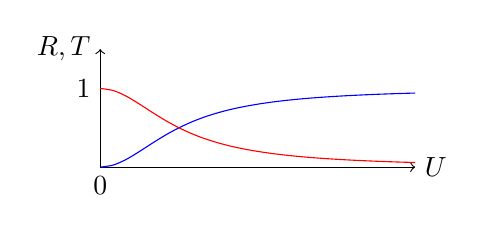
\begin{tikzpicture}
      \draw[->] (0,0) -- (4,0) node[right] {$U$};
      \draw[->] (0,0) -- (0,1.5) node[left] {$R,T$};
      \draw[domain=0:4,smooth,variable=\x,blue] plot ({\x},{\x^2/(\x^2+1)});
      \draw[domain=0:4,smooth,variable=\x,red] plot ({\x},{1/(\x^2+1))});
      \draw (0,0) node[below]{0};
\draw (0,1) node[left]{1};
\end{tikzpicture}
\end{center}
\end{enumerate}
\end{ans}
\newpage
\begin{qns}[Hybrid]\leavevmode
\begin{enumerate}[label=(\alph*)]
\item Show how the method of separation of variables can be used to solve the time-independent Schrodinger equation for the three-dimensional potential\hfill\textbf{[3]}
$$V=\frac{m}{2}(\omega_x^2x^2+\omega_y^2y^2+\omega_z^2z^2)$$
\item Explain what is meant by a conserved quantity and give conditions on the constants $\omega_x$, $\omega_y$, and $\omega_z$ such that the operators
\begin{enumerate}[label=(\roman*)]
\item $x\frac{\partial}{\partial y}-y\frac{\partial}{\partial x}$
\item $(x\frac{\partial}{\partial y}-y\frac{\partial}{\partial x})^2+(x\frac{\partial}{\partial z}-z\frac{\partial}{\partial x})^2+(z\frac{\partial}{\partial y}-y\frac{\partial}{\partial z})^2$
\end{enumerate}
are conserved. Explain your reasoning.\hfill\textbf{[4]}\\[5pt]
From now on, you may assume that $\omega_x=\omega_y=\omega_z=\omega$.
\item Write down the energy levels for a single electron moving in the potential and show that a suitable wavefunction for the first excited state takes the form $\psi=Axe^{-\alpha(x^2+y^2+z^2)}$ Find the value of $\alpha$.\hfill\textbf{[5]}
\item Calculate the uncertainty, $\Delta x$, in the $x$-coordinate in the first excited state and compare your answer with the amplitude of a classical oscillator with the same energy.\hfill\textbf{[4]}
\begin{mdframed}
\color{darkblue}{Hint: Use $\int_{-\infty}^\infty x^4e^{-2x^2}dx=\frac{3}{4}\int_{-\infty}^\infty x^2e^{-2x^2}dx$.}
\end{mdframed}
\item Now consider a system of nine non-interacting electrons moving in the potential. What are the energies of the ground state and of the first excited state?\hfill\textbf{[4]}
\end{enumerate}
\end{qns}
\begin{ans}\leavevmode
\begin{enumerate}[label=(\alph*)]
\item The Hamiltonian is
$$H=-\frac{\hbar^2}{2m}\bigg(\frac{\partial^2}{\partial x^2}+\frac{\partial^2}{\partial y^2}+\frac{\partial^2}{\partial z^2}\bigg)+\frac{1}{2}m(\omega_x^2x^2+\omega_y^2y^2+\omega_z^2z^2)$$
By separation of variables $\psi(x,y,z)=X(x)Y(y)Z(z)$, we have
$$-\frac{\hbar^2}{2m}\bigg(\frac{X''}{X}+\frac{Y''}{Y}+\frac{Z''}{Z}\bigg)+\frac{1}{2}m(\omega_x^2x^2+\omega_y^2y^2+\omega_z^2z^2)=E:=E_x+E_y+E_z$$
This gives three separate linear ordinary differential equations, which can be solved separately.
\item A conserved quantity is one whose expectation value does not change with time. By Ehrenfest Theorem, the rate of change of the expectation of an arbitrary operator $\hat{A}$ is
$$\frac{d\langle\hat{A}\rangle}{dt}=\frac{i}{\hbar}\langle[\hat{H},\hat{A}]\rangle+\bigg\langle\frac{\partial\hat{A}}{\partial t}\bigg\rangle$$
For $\frac{d\langle\hat{A}\rangle}{dt}$=0, we require $\langle\frac{\partial\hat{A}}{\partial t}\rangle=0$ and $[\hat{H},\hat{A}=0$.
\begin{enumerate}[label=(\roman*)]
    \item $x\frac{\partial}{\partial y}-y\frac{\partial}{\partial x}\propto\hat{L}_z$. For $\hat{L}_z$ to be conserved, $[\hat{L}_z,\hat{H}]=0$, i.e. the Hamiltonian is invariant under arbitrary rotations about the $z$-axis, i.e. $\omega_y=\omega_x$.
    \item $(x\frac{\partial}{\partial y}-y\frac{\partial}{\partial x})^2+(x\frac{\partial}{\partial z}-z\frac{\partial}{\partial x})^2+(z\frac{\partial}{\partial y}-y\frac{\partial}{\partial z})^2\propto\hat{L}^2$. For $\hat{L}^2$ to be conserved, $[\hat{L}^2,\hat{H}]=0$, i.e. the Hamiltonian is invariant under arbitrary rotations about any axis, i.e. $\omega_x=\omega_y=\omega_z$.
\end{enumerate}
\item $E=E_x+E_y+E_z=\frac{1}{2}\hbar\omega(n_x+n_y+n_z+1.5)$. To check $\psi$ is an eigenstate, we compute $\frac{\partial^2}{\partial x^2}\psi=(-6\alpha+4\alpha^2x^2)\psi$, $\frac{\partial^2}{\partial y^2}\psi=(-2\alpha+4\alpha^2y^2)\psi$ and $\frac{\partial^2}{\partial z^2}\psi=(-2\alpha+4\alpha^2z^2)\psi$ and compare with $\hat{H}\psi=E\psi$. This gives 
$$-4\alpha^2\frac{\hbar^2}{2m}+\frac{1}{2}m\omega^2=0\implies\alpha=\frac{m\omega}{2\hbar}$$
and $E=-\frac{\hbar^2}{2m}(-10\alpha)=\frac{5\hbar^2\alpha}{m}=\frac{5}{2}\hbar\omega$. This is the same energy as a state with $(n_x,n_y,n_z)$ being $(1,0,0)$, $(0,1,0)$ and $(0,0,1)$, i.e. the first excited state.
\item The expectations are
$$\langle\hat{x}^2\rangle=\int_{-\infty}^\infty|A|^2x^4e^{-\alpha x^2}dx\int_{-\infty}^\infty\int_{-\infty}^\infty e^{-\alpha(y^2+z^2)}dydz=\frac{3}{4\alpha}\int_{-\infty}^\infty |A|^2x^2e^{-\alpha x^2}dx\int_{-\infty}^\infty\int_{-\infty}^\infty e^{-\alpha(y^2+z^2)}dydz$$
$$\langle\hat{x}\rangle=\int_{-\infty}^\infty|A|^2x^3e^{-\alpha x^2}dx\int_{-\infty}^\infty\int_{-\infty}^\infty e^{-\alpha(y^2+z^2)}dydz=0$$
since the integrand is odd and the integral has symmetric limits, and the normalization constant is defined as $1=\int_{-\infty}^\infty |A|^2x^2e^{-\alpha x^2}dx\int_{-\infty}^\infty\int_{-\infty}^\infty e^{-\alpha(y^2+z^2)}dydz$. Thus, $\langle x^2\rangle=\frac{3}{4\alpha}$ and $\Delta x=\frac{1}{2}\sqrt{\frac{3}{\alpha}}=\sqrt{\frac{3\hbar}{2m\omega}}$. For a classical harmonic oscillator of energy $E=\frac{5}{2}\hbar\omega$, we have $\frac{5}{2}\hbar\omega=\frac{1}{2}m\omega^2a^2\implies a=\sqrt{\frac{5\hbar}{m\omega}}$. Hence, $\frac{\Delta x}{a}=\sqrt{\frac{3}{10}}\approx 0.547$, i.e. the particle spends more than half the time in the classical region.
\item Each state has a spin degeneracy of 2, since the spin of electrons is $\frac{1}{2}$. For the single particle states, the lowest eight states (labelled by ($n_x,n_y,n_z)$) are
\begin{itemize}
    \item $(0,0,0)$, $E=\frac{3}{2}\hbar\omega$, degeneracy is $1\times2=2$;
    \item $(1,0,0)$, $E=\frac{5}{2}\hbar\omega$, degeneracy is $3\times 2=6$;
    \item $(1,1,0)$ and $(2,0,0)$ have $E=\frac{7}{2}\hbar\omega$, degeneracy is not important, since only one of the few possible states can be occupied.
\end{itemize}
For the nine-particle ground state:
\begin{itemize}
    \item both single-particle ground state will be occupied;
    \item all six single-particle first excited state will be occupied;
    \item only one of the single-particle second excited state will be occupied.
\end{itemize}
The total energy is $(\frac{3}{2}\times 2+\frac{5}{2}\times 6+\frac{7}{2})\hbar\omega=\frac{43}{2}\hbar\omega$. To get the first excited state for the nine-particle system, one of the electrons in the single-particle first excited state will be promoted to a single-particle second excited state, or the electron already in the single-particle second excited state promoted into the single-particle third excited state. Either way the energy change is the same, so we an additional $\hbar\omega$.
\end{enumerate}
\end{ans}
\newpage
\subsubsection{Section C}
\begin{qns}[QM Essay]
Write an essay on the postulates of quantum mechanics and the experiments that gave rise to them. Include discussions of the photoelectric effect, and the Stern-Gerlach and Davisson-Germer experiments. \hfill\textbf{[20]}
\end{qns}
\begin{ans}
Quantum physics was a revolution in modern physics in the 19th century. The fundamental revolution is the idea brought forth by Max Planck that electromagnetic radiation is quantized, i.e. light are packets of fixed energy called photons. To motivate this postulate, we begin with a discussion of the photoelectric effect.\\[5pt]
In 1887, Hertz discovered that the electrons were observed to be ejected from the metal when the metal was irradiated with light. Classically, we expect:
\begin{itemize}
\item Since the intensity of an electromagnetic wave is proportional to the square of its amplitude, any frequency with sufficiently high intensity can supply the necessary energy to free the electron from the metal.
\item For low intensity, an electron will keep on absorbing energy at a continuous rate and hence given sufficient amount of time, the electron will gain sufficient energy to leave the metal.
\item Electron's kinetic energy should depend on the intensity of the light source. More intense radiation will give the electron more energy.
\end{itemize}
However, the observations made were completely opposite.
\begin{itemize}
\item If the frequency of the incident radiation is smaller than the metal's threshold frequency, which is dependent on the metal, no electron can be emitted regardless of the radiation's intensity.
\item No matter how low the intensity of the incident radiation, electrons will be ejected instantly the moment the frequency of the radiation exceeds the threshold frequency of the metal.
\item The kinetic energy of the ejected electron depends on the frequency but not the intensity of the beam. In fact, the kinetic energy increases linearly with the incident frequency.
\item Moreover, at any frequency above the threshold frequency, the number of electrons ejected increases with the intensity of the light but does not depend on the light's frequency. Hence, the magnitude of the photoelectric current generated is proportional to the intensity of the light.
\end{itemize} 
Based on Planck's postulate, Einstein gave a theoretical explanation for the photoelectric effect in 1905.
\begin{itemize}
\item The incident radiation of frequency $f$ consists of photons of energy $hf$. Electrons gain energy by completely absorbing one of these photons, irrespective of the intensity of the incident radiation. This interaction can be instantaneous.
\item The threshold frequency $f_0$ of the metal is related to the work function of the metal $W$, which is defined as the minimum energy required to dislodge the electron from the metal. As long as the photon's energy is greater than the work function, the electron will be ejected. The remaining energy of the electron is the kinetic energy of the electron $K$.
$$hf=W+K=hf_0+\frac{1}{2}mv^2$$
\item The kinetic energy of the electron increases linearly with the incident frequency and is clearly independent of the intensity of the radiation. Moreover, it clearly shows that below the threshold frequency, no electron can be ejected from the metal.
\end{itemize}
Planck's postulate was relevant in other experiments and models, and has helped revolutionize our understanding of physics. Another instance is the Bohr's model where Bohr extended this idea and postulated that the angular momentum of electron's orbits are quantized. This result in discrete energy levels which accounts for the emission and absorption spectra of various chemicals, particularly Hydrogen. In these spectra, spectral lines were identified at fixed wavelengths which are explained as photon emission accompanied by the electrons transiting different energy levels.\\[5pt]
Next, we discuss the Davisson and Germer experiment to illustrate another revolution in modern physics. In 1927, Davisson and Germer scattered a $54eV$ monoenergetic beam of electrons from a Nickel crystal. The source and detector were symmetrically located with respect to the crystal's normal, similar to Bragg setup for X-ray diffraction of a crystal. Interestingly, electrons are scattered in all directions from the crystal, but a minima and maxima was found at $\theta = 35\degree$ and $\theta=50\degree$ respectively. This pattern persisted even when the intensity of the beam was so low that the incident electrons were sent one at a time. This result was very similar to Bragg's X-ray diffraction, i.e. $n\lambda=2d\sin\phi $ where $2\phi+\theta=\pi$.\\[5pt]
This result cannot be explained by the classical idea where electrons are strictly regarded as particles. The experiment thus suggested that electrons have wave-like properties. In the same year, Thomson diffracted electrons through a polycrystalline thin film and obtained diffraction rings. This result was very similar to diffracting light through the same film. Thomson thus confirm that electrons have wave-like properties.\\[5pt]
In fact, in the first decade of the 1800s, Young carried out his original double-slit experiment with light to show that the waves of light from the two slits interfered to produce a characteristic fringe pattern on a screen. Classically, we expect when both slits, in front of a source of particles, are open, the resultant intensity distribution is the sum of that corresponding to each slit. As for waves, an interference pattern is obtained since the amplitudes add and not the intensities.
$$|\psi_1+\psi_2|^2=|\psi_1|^2+|\psi_2|^2+2\text{Re}(\psi_1^*\psi_2)$$
where the last term becomes $2\sqrt{I_1I_2}\cos\delta$, where $\delta$ is the phase difference between $\psi_1$ and $\psi_2$, which results in an oscillating term. The double-slit experiment for electrons was performed by Claus J\"{o}nsson, where he demonstrated electron interference pattern for up to five slits. All these experiments suggest the idea that particles have wave-like behaviour which is apparent in the quantum regime. Since then particle interference has been demonstrated with neutrons, atoms and molecules as large as carbon-60 and carbon-70. Motivated by this dual property in light, de Broglie derived a relationship between wavelength and momentum of matter, known as the de Broglie relation.
$$p=\frac{h}{\lambda}$$
More importantly, the experiments suggest that all quantum particles could really be described by like a wave-like function, known as the wavefunction that encompasses all of its behaviour. This postulates that states of a quantum system correspond to non-zero elements of a complex vector space (Hilbert space $\mathcal{H}$) with $\psi$ and $\alpha\psi$ physically equivalent $\forall\alpha\in\mathbb{C}\backslash\{0\}$. In particular, the norm squared of the wavefunction gives the probability density.  This process of taking the square magnitude explains how this `interference' occurs, similar to that in waves:
$$|\psi_1+\psi_2|^2=|\psi_1|^2+|\psi_2|^2+2\text{Re}(\psi_1^*\psi_2)$$
\end{ans}
\newpage
\begin{qns}[QM Short Notes]
Write brief notes on two of the following:\hfill\textbf{[20]}
\begin{itemize}
    \item symmetries and conservation laws in quantum mechanics;
    \item the vibrational and rotational specific heat capacities of gases;
    \item blackbody radiation
\end{itemize}
\end{qns}
\begin{ans}\leavevmode
\subsubsection*{Symmetries and conservation laws in quantum mechanics:}
For all wavefunctions to stay normalized after a generic transformation, then this transformation must be represented by a unitary operator.
$$1=\langle\psi'|\psi'\rangle=\langle\psi|U^\dag U|\psi\rangle$$
By treating time evolution as a unitary operator, we can obtain the time-dependent Schr\"{o}dinger's equation.
We write $U(t)=e^{-iHt/\hbar}$ and we have $|\psi(t)\rangle=U(t)|\psi(0)\rangle$ and hence
$$|\psi(t+\delta t)\rangle-|\psi(t)\rangle=[U(t+\delta t)-U(t)]|\psi(0)\rangle=(U(\delta t)-1)U(t)|\psi(0)\rangle=\bigg(1-i\frac{\delta t}{\hbar}H-1\bigg)|\psi(t)\rangle$$
or equivalently, $i\hbar\frac{\partial}{\partial t}|\psi(t)\rangle=H(t)|\psi(t)\rangle$, which is the time-dependent Schr\"{o}dinger's equation.\\[5pt]
Likewise, instead of working with time-dependent states, we can notice $$\langle\psi(t)|\mathbf{Q_S}|\psi(t)\rangle=\langle\psi(0)|U^{-1}(t)\mathbf{Q_S}U(t)|\psi(0)\rangle$$ and hence work with $|\psi(0)\rangle$ using time-dependent operators $\mathbf{Q_H}(t)=U^{-1}(t)\mathbf{Q_S}U(t)$ via conjugation. This is known as the Heisenberg's picture, where states are time-dependent but operators vary with time. This is in contrast with the Schr\"{o}dinger's picture (states change by time-dependent Schr\"{o}dinger's equation but operators are time-independent).\\[5pt]
Suppose an operator $Q$ does not depend on $t$ even in the Heisenberg picture, i.e. $Q(t)=U^{-1}(t)QU(t)=Q$ $\forall t$ true iff $[Q,H]=0$. Such operators are said to be conserved. If $Q$ is Hermitian, then it is useful to choose its eigenstates to be a basis of our $H$ if $Q$ is conserved.\\[5pt]
Now suppose the Hamiltonian is invariant under some transformation represented by $U(\theta):~\mathcal{H}\rightarrow\mathcal{H}$ with generator $T$. Then $H'=U(\theta)^{-1}HU(\theta)=H$. The Hamiltonian is invariant under such transformations. Equivalently, for an infinitesimal symmetry transformation $T$, we must have
$$[H,T]=0$$
This is the same equation as for conserved quantities, so symmetries of a given $H(X,P,...)$ correspond to conserved quantities.\\[5pt]
Consider the example of the free particle, where its Hamiltonian $H=\frac{P^2}{2m}$ is invariant under translations and rotations, i.e. $[H,P]=0$ and $[H,J]=0$. So momentum $P$ and angular momentum $J$ will be conserved. 
\newpage
\subsubsection*{The vibrational and rotational specific heat capacities of gases:}
For a diatomic molecule, its vibrational motion is the same as that of a single mass moving in a central potential (quadratic for low energies). Classically, each degree of freedom (vibrational mode) has thermal energy $0.5k_BT$. Quantum mechanically, an oscillator has a range of discrete vibrational energy states with $E_n=(n+0.5)\hbar\sqrt{\alpha/\mu}$ where $\mu$ is the reduced mass of the diatomic molecule and $\alpha$ is the stiffness of the chemical bond. The average vibrational energy per molecule is
$$\langle E\rangle=\frac{1}{2}\hbar\omega+\frac{\sum_{n=1}^\infty n\hbar\omega e^{-n\hbar\omega\beta}}{\sum_{n=1}^\infty e^{-n\hbar\omega\beta}}$$
To solve that summation, let $Z=\sum_{n=1}^\infty e^{-n\hbar\omega\beta}=\frac{1}{1-e^{-\hbar\omega\beta}}$ be the partition function. We have
$$-\frac{\partial Z}{\partial\beta}=\sum_{n=1}^\infty n\hbar\omega e^{-n\hbar\omega\beta}=\frac{\hbar\omega e^{-\hbar\omega\beta}}{(1-e^{-\hbar\omega\beta})^2}$$
so $\langle E\rangle=0.5\hbar\omega+\frac{\hbar\omega}{e^{\hbar\omega\beta}-1}$, where the second term is the average energy of a quantum SHO lightly coupled to a heat bath of temperature $T$. The vibrational heat capacity of $N$ diatomic molecules is
$$C_{vib}=N\frac{\partial\langle E\rangle}{\partial T}=Nk_B\frac{\hbar^2\omega^2}{k_B^2T^2}\frac{e^{\hbar\omega/k_BT}}{(e^{\hbar\omega/(k_BT)}-1)^2}$$
$C_{vib}\rightarrow NK_B$ as $T\rightarrow\infty$. It approaches the classical value at the temperature $\hbar\omega/k_B$.\\[5pt]
The diatomic molecule can be modelled as a rigid rotor, where its rotational behaviour is the same as that of a
single mass acting as a rigid rotor at a fixed distance
from the origin.
$$E=\frac{L^2}{2I}$$
where $I$ is the moment of inertia of the molecule about its centre of mass, i.e. $I=2\mu R^2$, where $R$ is the bond length. The energy is quantized $E_l=\frac{\hbar^2}{2I}l(l+1)$ with degeneracy $2l+1$. $\frac{\hbar^2}{2I}$ is the rotational constant. The mean rotational energy per rotor is
$$\langle E\rangle=\frac{\sum_l\frac{l(l+1)\hbar^2}{2I}(2l+1)e^{-l(l+1)\hbar^2/(2Ik_BT)}}{\sum_l(2l+1)e^{-l(l+1)\hbar^2/(2Ik_BT)}}$$
Unlike the vibrational case, this does not simplify easily. We can find the rotational heat capacity of $N$ molecules, i.e. $C_{rot}=N\frac{\partial\langle E\rangle}{\partial T}$. $\lim_{T\rightarrow0}C_{rot}=0$ while $\lim_{T\rightarrow\infty}C_{rot}=R$. There is, however, a characteristic temperature of rotation, i.e. $\frac{\hbar^2}{2Ik_B}$.\\[5pt]
These observations underpin the spectroscopic analysis
of diatomic gases. For each degree of freedom, there is an approximate critical temperature at which it "thaws" ("unfreezes") and becomes active, thus being able to hold heat energy. For the rotational degrees of freedom, the thawing temperature is usually a few tens of kelvins (although with a very light molecule such as hydrogen the rotational energy levels will be spaced so widely that rotational heat capacity may not completely "unfreeze" until considerably higher temperatures are reached). Vibration modes of diatomic molecules generally start to activate only well above room temperature. This results in a step-like temperature dependence of the heat capacities.
\newpage
\subsubsection*{Blackbody radiation:}
An idealized blackbody absorbs all of the incoming radiation. When the blackbody is in thermal equilibrium with its surroundings, it radiates as much energy as it absorbs. Hence, a blackbody is a perfect absorber and perfect emitter. The maximum intensity of this radiation depends on its frequency and on the temperature of the blackbody.\\[5pt]
A practical blackbody can be constructed by taking a hollow cavity whose internal metallic walls perfectly reflect electromagnetic radiation. The cavity also has a very small hole on its surface. Radiation that enters through the hole will be trapped inside the cavity and gets completely absorbed after successive reflections on the inner surfaces of the cavity. The hole behaves as a perfect absorber and emitter.\\[5pt]
When a solid is subjected to infrared radiation, a solid object glows and emits thermal radiation. As the temperature increases, the object becomes red, then yellow, then white. This emission of thermal radiation consists of a continuous distribution of frequencies ranging from infrared to ultraviolet, and peak at a wavelength dependent on its temperature (determined by Wien's Law). This is in stark contrast to the radiation emitted by heated gases, which is a discrete distribution spectrum (a few sharp, narrow, colored lines on a dark background). Stefan-Boltzmann Law states that the total intensity $I$ (power per unit surface area) radiated by a glowing object of temperature $T$ is
$$I=a\sigma T^4$$
where $\sigma$ is the Stefan-Boltzmann constant ($5.67\times10^{-8}Wm^{-2}K^{-4}$) and the coefficient $a$ (where $0<a<1$) is $1$ for a perfect blackbody. Accounting for blackbody radiation has been a mystery for many decades in the 19th to 20th century. Classical attempts include
\begin{itemize}
\item (1894) Wien's formula empirically fits the high frequency data but fails in the low frequency regime: $u(f,T)=\alpha f^3e^{-\frac{\beta f}{T}}$
\item In 1900, Rayleigh focused on understanding the nature of the electromagnetic radiation inside the cavity (which was modelled as a blackbody). He considered the radiation to consist of standing waves of temperature $T$ with nodes at the metallic surfaces. These standing waves are harmonic oscillations of a large number of electrons present in the walls of the cavity.\\[5pt]
When the cavity is in thermal equilibrium, the electromagnetic density inside the cavity is equal to the energy density of the charged particles in the walls of the cavity, The number of standing waves (modes) of the radiation in the frequency interval $f$ to $f+df$ is $N(f)=\frac{8\pi f^2}{c^3}$. The average energy of the oscillators present on the cavity walls can be determined using the equipartition theorem of classical thermodynamics, which is $kT$. Thus, the energy density per unit frequency (given by Rayleigh-Jeans formula) is $u(f,T)=\frac{8\pi f^2}{c^3}kT$. 
This fits well for low frequency regime but fails for high frequency, which diverges to infinity. Hence, this problem was termed as the ``ultraviolet catastrophe''.
\end{itemize}
In reality, the arguments put forth by both Wien and Rayleigh were erroneous simply because they assumed the energy exchange between radiation and matter is continuous. Planck, on the other hand, put forth an unprecedented argument using the postulate that the energy of the radiation emitted by the oscillators are integer multiples of hf, where $h$ is the Planck's constant.
The average energy for a quantized oscillator is thus
$$
\big \langle E \big \rangle = \frac{\sum_{n=0}^{\infty} nhfe^{-\frac{nhf}{kT}}}{\sum_{n=0}^{\infty}e^{-\frac{nhf}{kT}}}=\frac{hf}{e^{\frac{hf}{kT}}-1}$$
Hence we obtained the Planck distribution:
$$u(f,T)=\frac{8\pi f^2}{c^3}\frac{hf}{e^{\frac{hf}{kT}}-1}$$
Planck's distribution gives an exact fit for the entire frequency distribution. The total energy density can be found by integrating over the whole spectrum,
$$
\int_{0}^{\infty}u(f,T)df=\frac{8\pi h}{c^3}\int_{0}^{\infty}\frac{f^3}{e^{\frac{hf}{kT}}-1}df=\frac{8\pi^5 k^4T^4}{15h^3c^3}=\frac{4}{c}\sigma T^4$$
where $\sigma = \frac{2\pi^5 k^4}{15h^3c^2}$. In this way, Planck's relation leads to a finite total energy density of the radiation emitted by a blackbody, hence avoiding the ultraviolet catastrophe.
In the limit of very low frequencies $hf<<kT$, 
$$
u(f,T)\approx\frac{8\pi f^2}{c^3}\frac{hf}{\frac{hf}{kT}}=\frac{8\pi f^2}{c^3}kT
$$
On the other hand, in the limit of very high frequencies $hf>>kT$, the denominator will become very small
$$
u(f,T)=\frac{8\pi f^2}{c^3}\frac{hfe^{-\frac{hf}{kT}}}{1-e^{-\frac{hf}{kT}}}\approx\frac{8\pi hf^3}{c^3}e^{-\frac{hf}{kT}}$$
We can find the peak wavelength using Wien's Displacement Law, which relates the peak wavelength $\lambda_{max}$ of the radiation emitted by a black body of temperature $T$.
$$\lambda_{max}=\frac{2898.9\times 10^{-6}}{T}$$
The Wien's Distribution (black curve) do agree with Planck's Distribution for low frequencies ($f\rightarrow 0$) whereas the Rayleigh-Jeans' Distribution (blue curve)do agree with Planck's Distribution for high frequencies ($f\rightarrow\infty$). The Wien's Law helps us to determine the frequency where the energy density per unit frequency peaks at, given a constant temperature $T$.
\begin{center}
\begin{tikzpicture}
      \draw[->] (0,0) -- (8,0) node[right] {$f$};
      \draw[->] (0,-1) -- (0,3) node[left] {$u(f,T)$};
      \draw[domain=0:1.5,smooth,variable=\x,black] plot ({\x},{\x^2});
      \draw[domain=3:8,smooth,variable=\x,blue] plot ({\x},{\x^3 *exp(-\x)});
      \draw[domain=0.1:8,smooth,variable=\x,red] plot ({\x},{\x^3/(exp(\x)-1)});
      \draw (0,0) node[left]{0};
    \draw (3,0) node[below]{$f_{\text{max}}$};
\end{tikzpicture}
\end{center}
For a higher temperature (blue), the energy density increases while the frequency of maximum energy density increases.
\begin{center}
\begin{tikzpicture}
      \draw[->] (0,0) -- (8,0) node[right] {$f$};
      \draw[->] (0,-1) -- (0,3) node[left] {$u(f,T)$};
 \draw[domain=0.1:8,smooth,variable=\x,blue] plot ({\x},{(\x)^3/(exp(0.9*\x)-1)});
      \draw[domain=0.1:8,smooth,variable=\x,red] plot ({\x},{\x^3/(exp(\x)-1)});
      \draw (0,0) node[left]{0};
    \draw (3,0) node[below]{$f_{\text{max}}$};
\end{tikzpicture}
\end{center}
\end{ans}
\newpage
\subsubsection{Section D}
\begin{qns}[Op-Amp and Filters]\leavevmode
\begin{enumerate}[label=(\roman*)]
\item What does it mean for an operational amplifier (op-amp) to be “ideal”? When analyzing the response of a circuit containing an op-amp with negative feedback, what rules follow from approximating the op-amp as ideal?\hfill\textbf{[5]}
\item Consider the circuit shown below. An AC voltage of angular frequency $\omega$ is applied at $V_{in}$. Assuming an ideal op-amp, show that
$$\bigg|\frac{V_{out}}{V_{in}}\bigg|^2=\bigg(\frac{R_2}{R_1}\bigg)^2\frac{\omega^2\tau_1^2}{(1-\omega^2\tau_1\tau_2)^2+\omega^2(\tau_1+\tau_2)^2}$$
where $\tau_1=R_1C_1$, $\tau_2=R_2C_2$.\hfill\textbf{[5]}
\begin{figure}[H]
    \centering
    \includegraphics[scale=0.75]{2013P1D12Q.PNG}
\end{figure}
\item Sketch $|V_{out}/V_{in}|^2$ as a function of $\omega$, quantifying characteristic features of the function, and highlighting the behavior at low and high $\omega$ in the cases $\tau_1>>\tau_2$ and $\tau_2>>\tau_1$.\hfill\textbf{[5]}
\item This circuit could be used as a band-pass filter. How would you choose the components to achieve a sharp pass-band? In a circuit with a very sharp band, what ratio of which components determines the maximum amplification?\hfill\textbf{[3]}
\item With real components, explain what differences, especially at high $\omega$, you would expect compared with the ideal behavior above.\hfill\textbf{[2]}
\end{enumerate}
\end{qns}
\begin{ans}\leavevmode
\begin{enumerate}[label=(\roman*)]
\item An ideal operational amplifier have
\begin{itemize}
    \item infinite input impedance;
    \item infinite gain with zero phase shift at all frequencies, i.e. purely real;
    \item zero output impedance, i.e. device can supply arbitrary large currents and still maintain the prescribed value of $V_{out}$;
    \item no upper limit on the magnitude of the output voltage.
\end{itemize}
If the ideal operational amplifier is configured with negative feedback (so as to achieve a stable self-consistent solution), then the Golden Rules state
\begin{itemize}
    \item no potential difference between the two inputs;
    \item positive and negative terminal draws no current.
\end{itemize}
\newpage
\item Label the junction in the vicinity of the (-) terminal to be node X. Conserve current at node X and assume (-) terminal does not draw current,
$$\frac{V_{in}-V_X}{\frac{1}{i\omega C_1}+R_1}=\frac{-V_{out}+V_X}{(\frac{1}{R_2}+i\omega C_2)^{-1}}$$
Also, $V_X=0$ since (-) terminal draws no current.
\begin{eqnarray}
\bigg|\frac{V_{out}}{V_{in}}\bigg|&=&\bigg|\frac{1}{\frac{1}{i\omega C_1}+R_1}\bigg|\bigg|\frac{1}{\frac{1}{R_2}+i\omega C_2}\bigg|\nonumber\\&=&\frac{1}{(-\frac{1}{i\omega C_1}+R_1)(\frac{-1}{i\omega C_1}+R_1)}\frac{1}{(\frac{1}{R_2}+i\omega C_2)(\frac{1}{R_2}-i\omega C_2)}\nonumber\\&=&\frac{\omega^2C_1^2R_1^2}{R_1^2+R_1^4\omega^2C_1^2}\frac{R_2^2}{1+\omega^2C_2^2R_2^2}\nonumber\\&=&\frac{R_2^2}{R_1^2}\frac{R_1^2\omega^2C_1^2}{(1+R_1^2\omega^2C_1^2)(1+R_2^2\omega^2C_2^2}\nonumber\\&=&\frac{R_2^2}{R_1^2}\frac{\omega^2\tau_1^2}{(1-\omega^2\tau_1\tau_2)^2+\omega^2(\tau_1+\tau_2)^2}\nonumber
\end{eqnarray}
where $(1-\omega^2\tau_1\tau_2)^2+\omega^2(\tau_1+\tau_2)^2=1+\omega^4\tau_1^2\tau_2^2+\omega^2\tau_1^2+\omega^2\tau_2^2$.
\item 
$$\lim_{\omega\rightarrow 0}\bigg|\frac{V_{out}}{V_{in}}\bigg|^2=0=\lim_{\omega\rightarrow\infty}\bigg|\frac{V_{out}}{V_{in}}\bigg|^2$$
The graph thus starts from zero at $\omega=0$, peaks at a certain value, and decays to zero as $\omega\rightarrow\infty$. The maximum value of $|\frac{V_{out}}{V_{in}}|^2$ is $\frac{R_2^4}{R_1^4}\frac{\tau_1^4}{(\tau_1+\tau_2)^4}$ and this occurs when $\omega^{-2}=\tau_1\tau_2\implies\omega=\frac{1}{\sqrt{\tau_1\tau_2}}$. The peak value depends on whether $\tau_1>>\tau_2$ or $\tau_2>>\tau_1$, which respectively are: 
$$\bigg|\frac{V_{out}}{V_{in}}\bigg|\rightarrow\frac{R_2^2}{R_1^2}\frac{\tau_1^2}{(\omega^{-1}-\omega\tau_1\tau_2)^2+\tau_1^2}\rightarrow\frac{R_2^2}{R_1^2}$$
$$\bigg|\frac{V_{out}}{V_{in}}\bigg|\rightarrow\frac{R_2^2}{R_1^2}\frac{\tau_1^2}{\tau_2^2}=\frac{C_1^2}{C_2^2}$$
\item The half power points occur at $|\frac{V_{out}}{V_{in}}|=\frac{R_2^2}{2R_1^2}\frac{\tau_1^2}{(\tau_1+\tau_2)^2}$, and so removing the factors $\frac{R_2^2}{R_1^2}\tau_1^2$,
$$\frac{1}{(\omega^{-1}-\omega\tau_1\tau_2)^2+(\tau_1+\tau_2)^2}=\frac{1}{2(\tau_1+\tau_2)^2}\implies1-\omega^2\tau_1\tau_2=\pm\omega(\tau_1+\tau_2)$$
$$\implies \omega_\pm=\frac{\mp(\tau_1+\tau_2)\pm\sqrt{(\tau_1+\tau_2)^2+4\tau_1\tau_2}}{2\tau_1\tau_2}$$
For a sharp band, we need to minimize $\omega_+-\omega_-$, i.e. keep it as small as possible, compared to the mean $\frac{\omega_++\omega_-}{2}$. This occurs when $\tau_1=\tau_2\implies\frac{R_1}{R_2}=\frac{C_2}{C_1}$.
\item At high $\omega$ and with real components, $A$ is not real, i.e. a phase lag occur. This becomes a significant fraction of the period as $\omega\rightarrow\infty$, which leads to the undesirable inter-conversion between positive and negative feedback. Golden rules will thus not apply. Further, real amplifiers have internal frequency compensation such that $\lim_{\omega\rightarrow\infty}|A|=0$.
\end{enumerate}
\end{ans}
\newpage
\begin{qns}[Expt Mthds Short Notes]
Write brief notes on two of the following:\hfill\textbf{[20]}
\begin{itemize}
    \item causes of systematic errors and methods to eliminate them;
    \item `likelihood' and Bayes' theorem, including how they are applied to experimental data analysis;
    \item reducing unwanted environmental thermal effects in an experiment.
\end{itemize}
\end{qns}
\begin{ans}\leavevmode
\subsubsection*{Causes of systematic errors and methods to eliminate them:}
Systematic errors are broadly due to (i) inaccurate instruments, (ii) apparatus that differs from some assumed form, (iii) incorrect theory, that is, there are some effects present that are not taken into account. It is a good rule that whenever there is an apparent symmetry in the apparatus, reversing some quantity or interchanging any two components should in theory have no effect.
\begin{itemize}
    \item Study the equipment and measurement instruments beforehand to identify any zero errors and correct for them. Also, calibrate the instruments. If necessary, measure the same quantity with different equipment that may have been calibrated differently.
    \item Check the experimental set-up by measuring different quantities to make sure they are consistent with the desired experimental setup.
    \item Null methods can be used, where the indicating device need not be linear or well-calibrated and we attempt to make a measurement based on the indicating device coming to a null state.
    \item We can make the same measurement at different times to observe if there are any changes (or gradual drift) in the measured quantity due to environmental changes (ambient temperature) or changes in equipment (overheating) over time.
    \item We can make differential (difference) measurements so that the systematic error is cancelled out in the calculations.
\end{itemize}
\subsubsection*{'Likelihood' and Bayes' theorem, including how they are applied to experimental data analysis:}
Prior to any experiment, one usually has some prejudice as to the values of the model parameters, either on the basis of someone's else data or some other information. This is captured by $p($ model parameters $)$, which is known as the prior probability, i.e. our knowledge of the model parameters prior to performing the experiment. After the experiment, the extent to which certain model parameters are to be preferred will depend on whether the data measured could reasonably have been explained on the basis of those parameter values, which is captured by the likelihood function, $p($ Data| Model parameters $)$. By Bayes' Theorem, the posterior probability, i.e. our knowledge of the model parameters after performing the experiment, is
$$p(\text{ model parameters | Data })=\frac{p(\text{ Data | model parameters})\times p(\text{ model parameters })}{p(\text{Data})}$$
In the case of a uniform prior in the model parameters, the Bayesian parameter estimation is equivalent to the maximum likelihood approach which is to find the value of the vector of model parameters $\mathbf{a}$ that maximizes the likelihood function $\mathcal{L}(y_1,...,y_N|\mathbf{a})$. But $\mathcal{L}(y_1,...,y_N|\mathbf{a})$ measures $p(\text{data}|\mathbf{a})$, which is different from what we want, i.e. $p(\mathbf{a}|\text{data})$. 
\subsubsection*{Reducing unwanted environmental thermal effects in an experiment:}
Heat transfer between the experiment and the environment is sometimes undesirable. To minimize the impact of this, we shield the equipment thermally. To minimize heat transfer via evaporation, one can use a lid to cover the setup, preventing vapor from escaping. To minimize conduction, one could insulate the entire setup with styrofoam (which is a poor heat conductor). To minimize convection currents from setting up within the setup, conduct the experiment in vacuum. Lastly, to prevent radiative losses or gains, use a thin aluminium foil to wrap up the setup.
\end{ans}
\newpage
\subsection{Paper 2}
\subsubsection{Section A}
\begin{qns}[Resolution]
An interferometric array of radio telescopes operates at a frequency of $1.5\times10^{10}$ Hz and has a longest baseline of 100m and a shortest baseline of 5 m. Estimate the angular resolution of the array and the largest angular scale to which it is sensitive.\hfill\textbf{[4]}
\end{qns}
\begin{ans}
We treat the array as one big dish with effective baseline as the diameter of the dish. We have a range of angular resolution based on the range of baseline. The angular resolution is
$$\Delta\theta=1.22\frac{\lambda}{D}=\frac{1.22(3\times10^8)}{1.5\times10^{10}\times D}$$
where $\Delta\theta(D=100)=2.44\times10^{-4}$ rad and $\Delta\theta(D=5)=4.88\times 10^{-3}$ rad.\hfill\textbf{[4]}
\end{ans}
\begin{qns}[Impedance]
Explain why many spectacle lenses appear slightly purple.\hfill\textbf{[4]}
\end{qns}
\begin{ans}
The lens coating has a refractive index being the geometric mean of that of the lens itself and air. For perfect transmission, we require the lens coating to have thickness $\frac{\lambda}{4}$. To cover the entire visible spectrum, we choose green light, which lies in the middle. Blue and red have thus smaller transmission, so the reflected light seems purple.
\end{ans}
\begin{qns}[Wave Speed]
The speed of sound through air is measured to be 320 m/s. Estimate the air temperature.\hfill\textbf{[4]}
\begin{mdframed}
Hint: You may assume that air pressure $p$ is given by $p=nk_BT$, where $n$ is the number density of molecules, $T$ the temperature, and $k_B$ Boltzmann’s constant.
\end{mdframed}
\end{qns}
\begin{ans}
From ideal gas law, i.e. $pV=Nk_BT\implies p=\rho k_BT$, and that the wave speed of air is $v=\sqrt{\gamma p/\rho}$, we have $320=\sqrt{1.4\times(1.38\times10^{-19})T}\implies T=250$ K.
\end{ans}
\begin{qns}[Structure]
Explain the difference between fcc and bcc crystal lattices. How do these lattices look in reciprocal space?\hfill\textbf{[4]}
\end{qns}
\begin{ans}
For both lattices, the conventional unit cell consists of a cube with a lattice point at each corner. For bcc, there is an additional lattice point at the centre, while for the fcc there are additional lattice points on the centre of each face. Hence, there are 2 and 4 lattice points respectively per conventional unit cell. The reciprocal lattice of bcc is the fcc, and vice-versa.
\end{ans}
\begin{qns}[Transport]
Explain the Hall effect, and show how, by measuring the Hall coefficient, one can deduce the average number of free electrons per atom.\hfill\textbf{[4]}
\end{qns}
\begin{ans}
A steady current in the presence of a steady magnetic field (perpendicular to the direction of current flow) has no net force as the magnetic force $Bqv$ is opposed by the electric force $qE$ arising from a static potential difference due to a concentration gradient of charge carriers. Hence, $qE=qvB\implies E=vB$.\\[5pt]
Assume the field is uniform, then for a conductor of width $w$, the electric field is $E=\frac{V}{w}$. The current is $I=JA=nqvA$, with $A$ being the cross-sectional area. The Hall coefficient is
$$R_H=\frac{E}{JB}=\frac{vB}{nqvB}=\frac{1}{nq}$$
Together with the number density of atoms, we can determine the number of conduction electrons (each with charge $e$) per atom.
\end{ans}
\newpage
\subsubsection{Section B}
\begin{qns}[Impedance]\leavevmode
\begin{enumerate}[label=(\roman*)]
\item Given that the product $\text{Re}[A]\text{Re}[B]$ can be written as $\frac{1}{2}(A+A^*)\frac{1}{2}(B+B^*)$, where $A$ and $B$ are complex numbers and $^*$ denotes the complex conjugate, show that the time-averaged power for an oscillator subject to a force $\text{Re}[F]$ and having velocity $\text{Re}[u]$, where $F = F_0e^{i\omega t}$ and $u = u_0e^{i(\omega t+\phi)}$, is $\frac{1}{2}\text{Re}[Fu^*]$.\hfill\textbf{[4]}
\item A light string, of mass $\rho$ per unit length, is stretched along the $x$-axis under tension $T$. Show that small transverse displacements $\psi(x,t)$ satisfy the wave equation
$$\frac{\partial^2\psi}{\partial x^2}=\frac{1}{v^2}\frac{\partial^2\psi}{\partial t^2}$$
and give an expression for $v$ in terms of $\rho$ and $T$.\hfill\textbf{[5]}
\item Using the representation $\psi(x,t)=A_0e^{i(\omega t-kx)}$ for a transverse wave, show that the average power carried along the string by the wave is $\frac{1}{2}Z\omega^2A_0^2$ and briefly describe the meaning of $Z$.\hfill\textbf{[4]}
\item State the conditions satisfied by $\psi$ and $\frac{\partial\psi}{\partial x}$ at any point on the string.\hfill\textbf{[2]}
\item State the general expressions for the reflected and transmitted powers at an impedance boundary.\hfill\textbf{[2]}
\item What are these reflected and transmitted powers if: (a) the string density changes from $\rho_1$ at $x < 0$ to $\rho_2$ at $x > 0$; (b) the string is constrained in such a way that $\frac{\partial\psi}{\partial x}=0$ at $x = 0$ but $\psi$ is otherwise unconstrained?\hfill\textbf{[3]}
\end{enumerate}
\end{qns}
\begin{ans}\leavevmode
\begin{enumerate}[label=(\roman*)]
\item The power is $\text{Re}[F]\text{Re}[u]$
$$\frac{1}{4}(Fu+(Fu)^*+Fu^*+(Fu^*)^*)=\frac{1}{2}\text{Re}[Fu]+\frac{1}{2}\text{Re}[Fu^*]=\frac{1}{2}\text{Re}[F_0u_0e^{i2\omega t}]+\frac{1}{2}\text{Re}[F_0u_0^*]$$
Result is $\frac{1}{2}|F_0||u_0|\cos(2\omega t+\text{arg}(F_0)-\text{arg}(u_0))+\frac{1}{2}\text{Re}[Fu^*]$. The first term averages to zero, so the time-averaged $\langle P\rangle=\frac{1}{2}\text{Re}[Fu^*]$.
\item The net force on a string element between $x$ and $x+\Delta x$ is the tension in the string projected on the vertical. $F=T\sin\phi-T\sin\theta$. Assume the angles are small enough, such that $\sin\theta\approx\tan\theta=\frac{\partial y}{\partial x}$.
$$F=T\bigg(\frac{\partial y}{\partial x}(x+\Delta x)-\frac{\partial y}{\partial x}(x)\bigg)\implies\rho\Delta x\frac{\partial^2y}{\partial t^2}=T\Delta(\frac{\partial y}{\partial x})$$
Take $\Delta x\rightarrow0$ to give wave equation, where $v=\sqrt{T/\rho}$.
\item The force is $F=-T\frac{\partial\psi}{\partial x}=+ikT\psi$ and the velocity response is $u=\frac{\partial\psi}{\partial t}=i\omega\psi$. The time-averaged power is
$$\langle P\rangle=\frac{1}{2}\text{Re}[+ikT\psi(-i\omega\psi)]=\frac{1}{2}kT\omega|A_0|^2=\frac{1}{2}Z\omega^2|A_0|^2$$
where $Z=\frac{T\frac{\partial\psi}{\partial x}}{\psi}=\frac{kT}{\omega}$ is the impedance of the system.
\item $\psi$ and $\psi'$ are continuous at all points on the string.
\item The power reflection coefficient is $R=|\frac{Z_1-Z_2}{Z_1+Z_2}|^2$ while the power transmission coefficient is $\tau=1-R=\frac{4Z_1Z_2}{(Z_1+Z_2)^2}$ where $Z_1$ and $Z_2$ are the two impedances on either side of the boundary.
\item (a) We have $Z=\frac{kT}{\omega}=\sqrt{T\rho}$, then $R=(\frac{1-\sqrt{\rho_1/\rho_2}}{1+\sqrt{\rho_1/\rho_2}})^2$ and $\tau=\frac{4\sqrt{\rho_1\rho_2}}{(\sqrt{\rho_1+\rho_2})^2}$.\\[5pt]
(b) $Z_2=0\implies R=1,\tau=0$.
\end{enumerate}
\end{ans}
\newpage
\begin{qns}[Oscillation]\leavevmode
\begin{enumerate}[label=(\roman*)]
\item The equation for a damped, driven, harmonic oscillator can be represented by $m\ddot{x}+b\dot{x}+kx=\text{Re}[F_0e^{i\omega t}]$. Explain the terms in this equation.\hfill\textbf{[2]}
\item By substituting the trial solution $x=\text{Re}[Ae^{i\omega t}]$ into the above equation, show that $A = R(\omega)F_0$, where $R(\omega)$ is the response function\hfill\textbf{[2]}
$$R(\omega)=\frac{1}{k-m\omega^2+i\omega b}$$
\item Show that the angular frequency at which amplitude resonance occurs is\hfill\textbf{[4]}
$$\omega_{res}=\sqrt{\frac{k}{m}-\frac{b^2}{2m^2}}$$
\item Draw an annotated sketch of the magnitude of $R(\omega)$ as a function of $\omega$, and indicate clearly how $R(\omega)$ changes for different levels of damping.\hfill\textbf{[4]}
\item For the circuit shown below, in which $V=\text{Re}[V_0e^{i\omega t}]$, show that the equation for
\begin{figure}[H]
    \centering
    \includegraphics[scale=0.5]{2013P2B7Q.PNG}
\end{figure}
the charge on the capacitor can be represented by\hfill\textbf{[3]}
$$L\ddot{q}+R\dot{q}+\frac{q}{C}=V$$
\item If $\omega_{max}$ is the angular frequency at which the root-mean-square voltage across the resistor $R$ is a maximum, show that, for light damping, \hfill\textbf{[5]}
$$\omega_{max}-\omega_{res}=\frac{R^2}{4L}\sqrt{\frac{C}{L}}$$
\end{enumerate}
\end{qns}
\begin{ans}\leavevmode
\begin{enumerate}[label=(\roman*)]
\item $m$ is the mass of particle, $b$ is the frictional force per unit velocity, $k$ is restoring force per unit displacement, $F_0$ is the complex amplitude of driving force.
\item We have $-\omega^2Ame^{i\omega t}+i\omega Abe^{i\omega t}+kAe^{i\omega t}=F_0e^{i\omega t}\implies R(\omega)=\frac{A}{F_0}=\frac{1}{k-m\omega^2+i\omega b}$.
\item First substitute $\gamma=\frac{b}{m}$ and $\omega_0^2=\frac{k}{m}$. We see that the peak of $R(\omega)$ is
$$0=\frac{d}{d\omega}|R(\omega)|=-\frac{1}{2}\frac{-4\omega(\omega_0^2-\omega^2)+2\omega\gamma^2)}{[(\omega^2-\omega_0^2)^2+\omega^2\gamma^2]^{3/2}}$$
which give solutions $\omega=0$, $\omega=\infty$ and $\omega=\sqrt{\omega_0^2-0.5\gamma^2}$. The last answer is $\omega_{res}$.
\item  The smaller the $\gamma$ (proportional to extent of damping), and so the higher the amplitude and the resonant peak $\omega_{res}$ approaches $\omega_0$. No resonance is achieved for $\gamma\geq2$ (regimes that are not light damping). Below shows light damping (black), critical damping (blue), heavy damping (red).
\begin{center}
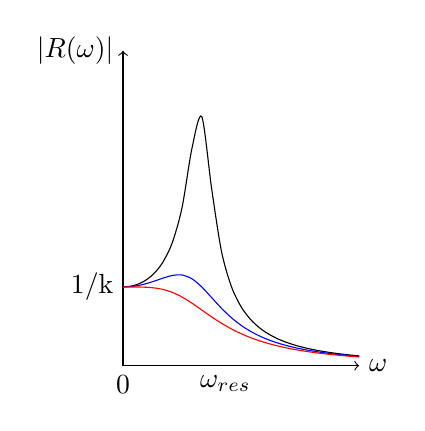
\begin{tikzpicture}
      \draw[->] (0,0) -- (3,0) node[right] {$\omega$};
      \draw[->] (0,0) -- (0,4) node[left] {$|R(\omega)|$};
      \draw[domain=0:3,smooth,variable=\x,black] plot ({\x},{1/sqrt((1-\x^2)^2+0.1*\x^2)});
      \draw[domain=0:3,smooth,variable=\x,blue] plot ({\x},{1/sqrt((1-\x^2)^2+\x^2)});
      \draw[domain=0:3,smooth,variable=\x,red] plot ({\x},{1/sqrt((1-\x^2)^2+2*\x^2)});
      \draw (0,0) node[below]{0};
\draw (0,1) node[left]{1/k};
\draw (1.3,0) node[below]{$\omega_{res}$};
\end{tikzpicture}
\end{center}
\item By Kirchoff's Voltage law,
$$V=IR+L\frac{dI}{dt}+\frac{q}{C}=\frac{dq}{dt}R+L\frac{d^2q}{dt^2}+\frac{q}{C}$$
and we obtain our desired differential equation.
\item Here, $\gamma=\frac{R}{L}$ and $\omega_0=\frac{1}{\sqrt{LC}}$. Invoking an earlier result, $\omega_{res}=\sqrt{\omega_0^2-0.5\gamma^2}=\sqrt{\frac{1}{LC}-\frac{R^2}{2L^2}}$. $\omega_{max}$ occurs when $\omega L=\frac{1}{\omega C}\implies\omega_{max}=\frac{1}{\sqrt{LC}}$. For light damping, i.e. $\frac{R^2C^2}{2L}<<1$:
$$\omega_{max}-\omega_{res}=\frac{1}{\sqrt{LC}}-\sqrt{\frac{1}{LC}-\frac{R^2}{2L^2}}\approx\frac{1}{\sqrt{LC}}\frac{R^2C}{4L}=\frac{R^2}{4}\sqrt{\frac{C}{L}}$$
\end{enumerate}
\end{ans}
\newpage
\begin{qns}[Dispersion]\leavevmode
\begin{enumerate}[label=(\roman*)]
\item Explain the term wavepacket, and define phase velocity and group velocity.\hfill\textbf{[3]}
\item For electromagnetic waves of frequency $f$ in a dispersive medium of refractive $n(f)$, the phase velocity is $c/n(f)$, where $c$ is the speed of light in vacuum. Show that the group velocity $u_g$ is given by \hfill\textbf{[4]}
$$\frac{c}{u_g}=n(f)+f\frac{dn(f)}{df}$$
A communications transmitter sends pulses of radiation of centre frequency $f_0=2\times10^{14}$ Hz and duration $10^{-10}$s at a rate of $10^9$ per second into an optical fibre. The fibre has refractive index $n(f)=1.5+\tau(f-f_0)$ where $\tau=3\times10^{-16}$ s. A receiver is connected to the other end of the fibre.
\item Justify the fact that the range of frequencies present in each transmitted pulse covers around $10^{10}$ Hz. \hfill\textbf{[1]}
\item Find the group velocity at the centre frequency, and estimate the range of group velocities present in each transmitted pulse.\hfill\textbf{[4]}
\item Explain what limits the useable length of this optical fibre, and estimate the maximum useable length in kilometres.\hfill\textbf{[6]}
\item A longer useable length could be obtained by fitting repeaters at intervals along the fibre. What must each of these repeaters do?\hfill\textbf{[2]}
\end{enumerate}
\end{qns}
\begin{ans}\leavevmode
\begin{enumerate}[label=(\roman*)]
\item A superposition of harmonic waves with different frequencies is called a wavepacket. This localizes the disturbance in space.\\[5pt]
Dispersive waves have the following dispersion relation: $\omega(k)$ that is not a constant, and is a function of $k$. Different wavelengths travel at different phase speeds. The phase velocity of a wave is the rate at which the phase of the wave propagates in space. This is the velocity at which the phase of any one frequency component of the wave travels, i.e. any harmonic wave: $v_p=\frac{\omega(k)}{k}$. The group velocity of a wave is the velocity of the interference maximum of a wavepacket. $v_g=\frac{\partial\omega(k)}{\partial k}|_{k=k_0}$ For a dispersive wave, $v_g\neq v_p$. In a non-dispersive media, the waves do not exhibit a dispersion relation.
\item We have $ck=n\omega$ for electromagnetic waves. Hence, 
$$c\frac{\partial k}{\partial\omega}=n+\omega\frac{\partial n}{\partial\omega}\implies\frac{c}{u_g}=n+2\pi f\frac{\partial n}{\partial(2\pi f)}=n+f\frac{dn}{df}$$
\item In the time domain, the signal $g(t)$ consists of a sine wave of frequency $f_0=2\times10^{14}$ Hz, multiplied by a top hat function of width $T_P=10^{-10}$ s (duration of pulse). This is then convolved with an infinite comb of delta functions with spacing $T_R=10^{-9}$ s (time interval between successive pulses). The Fourier transform of this signal $\tilde{g}(f)$ is:\\[5pt]
The carrier sine wave transforms to a delta function at $f_0$ (as well as a negative delta function at $-f_0$ if the oscillation is a sine wave). The top hat transforms to a sinc function $\frac{\sin(\pi fT_P)}{\pi fT_P}$. This sinc function has a zero at $\Delta f=\frac{1}{T_P}=10$ GHz, and another one at $-\Delta f$. When we convolve this sinc function with the delta function, it shifts it to be centred at $f_0$ with zeros at $f_0\pm \Delta f$. Finally, we multiply by the Fourier transform of the comb function (finely-spaced infinite comb of delta functions with spacing $\frac{1}{T_R}=1$ GHz).
\item 
$$n(f)=1.5+3\times10^{-16}(f-2\times10^{14})$$
$$\frac{c}{u_g}=1.5+\tau(f-f_0)+f\tau=1.5+\tau(2f-f_0)\implies u_g=\frac{3\times10^8}{1.5+3\times10^{-16}((2-1)2\times10^{14})}=1.92\times10^8 m/s$$
For $f_0\pm\Delta f$,
$$\Delta u_g=\frac{\partial u_g}{\partial f}\Delta f=-\frac{2\tau c}{(1.5+\tau(2f_0-f_0))^2}\Delta f\implies|\Delta u_g|=\frac{2(3\times10^{-16})(3\times10^8)10^{10}}{(1.5+3\times10^{-16}2\times10^{14})^2}=740m/s$$
So the group velocity is $(1.92\times10^8\pm 370)$ m/s.
\item The refractive index of the fibres result in the velocity of the wavepacket to be frequency dependent. As the wavepacket travels, the range of group speeds present cause the wavepacket to disperse. We have the distance to be $v_g(fast)T=v_g(slow)(T+T_R)$ and so
$$\frac{1.92\times10^8+370}{1.92\times10^8-370}=1+\frac{T_R}{T}$$
The distance is $(1.92\times10^8-370)T$ which gives 49.8 km.
\item Each repeater must re-emit the optical signal at the same frequency and same power.
\end{enumerate}
\end{ans}
\begin{qns}[Fraunhofer Diffraction]\leavevmode
\begin{enumerate}[label=(\roman*)]
\item A thin opaque sheet in the $x$-$y$ plane contains a transparent aperture. The aperture is described by an aperture function $h(x)$, where $x$ is the horizontal direction. The aperture is infinitely long in the vertical $y$ direction. If this aperture is illuminated by plane-wave, monochromatic light of wavelength $\lambda$ travelling in the $z$-direction, state the condition that the resulting diffraction is Fraunhofer rather than Fresnel.\hfill\textbf{[2]}
\item Starting from the conditions for the Fraunhofer regime, show that the light intensity that appears on a screen placed parallel to and after the aperture plane depends on a Fourier transform of $h(x)$.\hfill\textbf{[5]}
\item Consider a particular system illuminated as described, where the aperture is a slit of width $b$ in the $x$-direction. A very thin layer of glass, which reverses the phase of the light passing through it, is placed over the left-hand half of the slit. Show that the resulting intensity diffraction pattern on the screen in the Fraunhofer regime has an angular dependence proportional to
$$\frac{1}{\sin^2\theta}\sin^4\bigg(\frac{kb\sin\theta}{4}\bigg)$$
where $k=\frac{2\pi}{\lambda}$ and $\theta$ is the angle, at the aperture centre and in the $x$, $z$ plane, between the $z$ axis and a point on the screen.\hfill\textbf{[7]}
\item Draw an annotated sketch of this diffraction pattern.\hfill\textbf{[4]}
\item How would the diffraction pattern change if the thickness of the glass layer were doubled?\hfill\textbf{[2]}
\end{enumerate}
\end{qns}
\newpage
\begin{ans}\leavevmode
\begin{enumerate}[label=(\roman*)]
\item The Fraunhofer regime occurs when the variation in phase along the observation screen is approximately linear in the distance in the aperture plane. The quadratic and higher order variations can only be neglected if their extra path difference from one extreme of the aperture to another is very much less than half a wavelength. The Frensel regime occurs when the quadratic terms cannot be neglected, but the cubic and higher terms can.
\item By Huygen's principle, light incident on the aperture plane will be diffracted in all directions. Consider the ray that passes through the origin, and then to a distant observer. Consider another ray, passing through a point $x$ in the aperture plane, that also is diffracted towards the same distant observer. For the Fraunhofer approximation, we will assume that these rays are parallel. The extra path difference is given by $x\sin\theta$, and so we may represent the infinitesimal amplitude $d\psi$ passing through a strip of width $dx$ at position $x$ on the aperture plane that eventually reaches an observer at an angle $\theta$ to the straight through beam as $d\psi=Adx e^{i(k[X+x\sin\theta]-\omega t)}$, where $A$ is the amplitude per unit length incident on aperture, and $X$ is the distance from the origin of the aperture plane to the distant observer. The distant observer sees the sum of these
$$\psi_{tot}=\int_{-\infty}^\infty h(x)Ae^{i(kX-\omega t)}e^{ikx\sin\theta}d\theta=\sqrt{2\pi}Ae^{i(kX-\omega t)}\tilde{h}(k\sin\theta)$$
and so the observed intensity is $|\psi_{total}|^2\propto|\mathcal{F}[h(x)]|^2$, where we take the Fourier transform variable to be $q=k\sin\theta$.
\item The aperture function is
$$h(x)=[\delta(x-0.25b)-\delta(x+0.25b)]\otimes\text{rect}(x/0.5b)$$
By Convolution Theorem, the Fourier transform of $h(x)$ is
$$\mathcal{F}[h]=\frac{1}{\sqrt{2\pi}}(-e^{iqb/4}+e^{-iqb/4})\times\mathcal{F}[\text{rect}(x/0.5b)]\propto\sin(qb/4)\sinc(qb/4)$$
and so the intensity will be $\propto\sin^2(qb/4)\sinc^2(qb/4)=\frac{\sin^4(kb\sin\theta/4)}{\sin^2\theta}$.
\item Assuming the distance from the aperture to the screen is $L$, the points on the screen will be at a distance of $u=L\tan\theta$ from the straight through beam. Further, assume small angle approximation and that the Fraunhofer regime holds, then $I(u)\propto\sin^4(\pi bu/2L\lambda)\frac{1}{u^2}$. The intensity pattern (blue) will have a central zero, symmetric, oscillates like a $\sin$ curve modulated by a $1/u^2$ curve (black). Maxima are not exactly halfway between minima such that the peak will be slightly shifted towards $u=0$.
\pgfplotsset{ticks=none}
\begin{center}
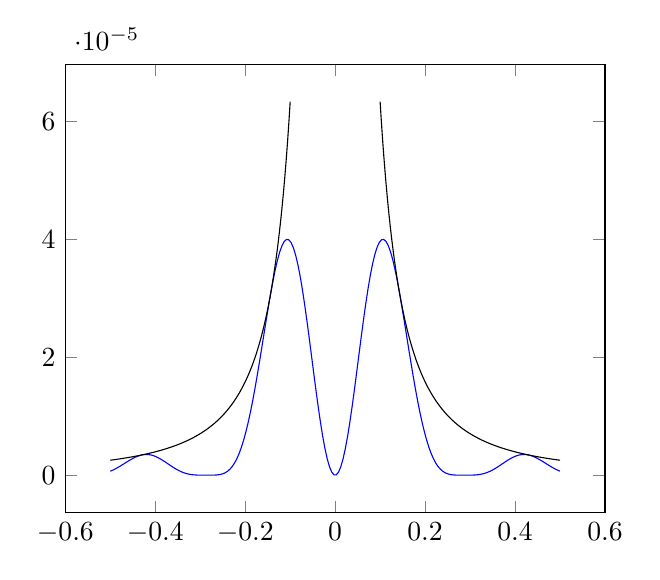
\begin{tikzpicture} 
    \begin{axis}[
    x label style={at={(axis description cs:0.5,-0.05)},anchor=north},
    y label style={at={(axis description cs:-0.05,.5)},anchor=south}]
      \addplot [domain = -0.5:0.5, samples = 200,color=blue]
      ({\x},{((sin(200*pi*\x))^2/(400*pi*\x))^2});
      \addplot [domain = -0.5:-0.1, samples = 200,color=black]
      ({\x},{1/(400*pi*\x)^2});
      \addplot [domain = 0.1:0.5, samples = 200,color=black]
      ({\x},{1/(400*pi*\x)^2});
 \end{axis}
\end{tikzpicture}
\end{center}
\item If the glass thickness is doubled, then the aperture function is $h(x)=\text{rect}(x/0.25b)$. With the extra $\pi$ phase shift, the diffraction pattern is $\sinc^2(kb\theta/2)$. Thus,  the spacing between minima on the screen will be half as big, and there will now be a central maximum rather than a central zero.
\end{enumerate}
\end{ans}
\newpage
\subsubsection{Section C}
\begin{qns}[Free Electron Model]\leavevmode
\begin{enumerate}[label=(\roman*)]
\item Outline the assumptions of the free-electron model of a solid.\hfill\textbf{[3]}
\item Assuming that electrons are confined to a 2D plane (as in graphene, for example), show that the density of states for the number of these electrons at each energy value is given by $g(\epsilon) = (A/2\pi)(m/\hbar^2)$ where $A$ is the area.\hfill\textbf{[5]}
\item Electrons are fermions and obey the Pauli exclusion principle. Calculate the maximum energy $\epsilon_F$ for $N$ electrons on a plane of area $A$ at $T = 0$ and sketch the diagram of occupied states.

\hfill\textbf{[6]}
\item By considering the probability that a state of energy $\epsilon$ is occupied, outline the derivation of the Fermi-Dirac probability distribution
$$p(\epsilon)=\frac{1}{e^{(\epsilon-\mu)k_BT}+1}$$
and demonstrate how the chemical potential $\mu$ is related to the Fermi energy $\epsilon_F$ at very low temperatures.\hfill\textbf{[6]}
\end{enumerate}
\end{qns}
\begin{ans}\leavevmode
\begin{enumerate}[label=(\roman*)]
\item The core electrons are assumed to be tightly bounded to the lattice sites and the delocalized electrons are free to move throughout the entire crystal, in  a uniform background potential due to the core electrons and the nuclei. 
\item For non-relativistic electrons, the dispersion relation is $\varepsilon=p^2/2m\implies d\varepsilon=pdp/m$. The momentum is quantized in both $x$ and $y$ directions. Impose periodic boundary conditions for a crystal of dimensions $L_x$ and $L_y$. 
$$L_{x,y}=n_{x,y}\lambda_{x,y},~n_x,n_y\in\mathbb{Z}^+\quad p_{x,y}=\frac{n_{x,y}h}{L_{x,y}}~\Delta p_x\Delta p_y=\frac{h^2}{_xL_y}$$
The number of states with a momentum of magnitude $p\in[p,p+dp]$ is the area of an annulus in momentum space of width $dp$ and radius $p$ divided by the area per state.
$$g(p)dp=\frac{2\pi pdp}{h^2/A}=\frac{A}{2\pi\hbar^2}pdp$$
bu $pdp=md\varepsilon$, so $g(\varepsilon)d\varepsilon=(Am/2\pi\hbar^2)d\varepsilon$, as desired.
\item Since electrons are spin $1/2$, each state can be occupied by two electrons with their spins paired anti-parallel. At $T=0$K, the Fermi energy $\varepsilon_F$ is the state with the highest energy. The number of states satisfy
$$N=\int_0^{\varepsilon_F}2g(\varepsilon)d\varepsilon=\frac{Am\varepsilon_F}{\pi\hbar^2}\implies\varepsilon_F=\frac{n\pi\hbar^2}{m}$$
Assume the real space lattice is a square with lattice parameter $a$. The area of the first Brillouin Zone is equal to the area of the circle of occupied states. For a divalent metal in the free electron model, we have the area of the circle to be equal of the square.
\item The first law of thermodynamics with particle exchange gives
$$dS=\frac{dU}{T}-\frac{\delta W}{T}-\frac{\mu}{T}dN$$
where $\delta W$ is the work done on the system such that $\delta W$ is an inexact differential. Assume $dA=0$ constant area, so $\delta W=pdA=0$, so we can treat the density of states $g(\varepsilon)$ as constant. If the system (one state of energy $\varepsilon_i$) is in the ground state and the environment (large reservoir of energy) has entropy $S_0=k_B\ln W_0$ where $W$ is the number of reservoir configurations. To excite the system, we need to transfer $\varepsilon_i$ of energy and one particle from the reservoir to the system. The corresponding entropy change in the system is
$$S_0+dS=S_0-(\varepsilon_i/T)-(\mu/T)(-1)\implies W=W_0e^{-(\varepsilon_i-\mu)/k_BT}$$
Normalize this by summing over all possible excited states (there is only one here) will give
$$p(\varepsilon)=\frac{W(\varepsilon)}{W(0)+W(\varepsilon)}=\frac{e^{-(\varepsilon-\mu)/k_BT}}{1+e^{-(\varepsilon-\mu)/k_BT}}=\frac{1}{e^{(\varepsilon-\mu)/k_BT}+1}$$
At low temperatures, there are no excited states occupied, and all states below $\varepsilon_F$ are definitely occupied, thus the chemical potential is $\mu=\varepsilon_F$. This results in the above probability distribution to be a step function ($p(\varepsilon)=1$ for $\varepsilon<\mu$ and 0 otherwise).
\end{enumerate}
\end{ans}
\begin{qns}[Phonons]\leavevmode
\begin{enumerate}[label=(\roman*)]
\item A string is composed of identical masses, each of mass $m$, each separated by a distance $a$, and connected by elastic springs of spring constant $\alpha$. Show that the frequency of longitudinal waves in this string is given by
$$\omega(q)=\sqrt{\frac{4\alpha}{m}}\bigg|\sin\bigg(\frac{qa}{2}\bigg)\bigg|$$
where $q$ is the wavevector.\hfill\textbf{[5]}
\item Sketch the dispersion relation of these waves and explain the meaning of the “first Brillouin zone”.\hfill\textbf{[4]}
\item Show how this analysis extends to the situation in which every second mass in this 1D lattice is replaced by a larger mass $M$. 
\begin{mdframed}
\color{darkblue}{Hint: This can be considered as a 1D diatomic lattice with a period $2a$.}
\end{mdframed}
In particular, show that the dispersion relation is
$$\omega^2=\frac{\alpha}{Mm}\bigg[M+m\pm\sqrt{(M+m)^2-4Mm\sin^2(qa)}\bigg]$$
demonstrating how the optical and acoustic phonon modes emerge, and explaining the difference in atomic motion between these two modes.\hfill\textbf{[6]}
\item Sketch the dispersion relation and show that the gap at the edge of the first Brillouin zone is equal to $\Delta\omega=\sqrt{2\alpha/m}-\sqrt{2\alpha/M}$.\hfill\textbf{[3]}
\item What would change in the spectra of phonon modes if the diatomic lattice were three-dimensional?\hfill\textbf{[2]}
\end{enumerate}
\end{qns}
\begin{ans}\leavevmode
\begin{enumerate}[label=(\roman*)]
\item Let the deviation from equilibrium of the $n$th mass be $u_n$. We model the small amplitude oscillatory motion as normal modes where all the linked masses vibrate at a single frequency. From Newton's second law, the equation of motion is
$$m\ddot{u}_n=-\alpha(u_n-u_{n+1})-\alpha(u_n-u_{n-1})$$
We seek solutions of the form $u_n=Xe^{i(\omega t-nqa)}$ where $q$ is the wavevector, $x_n=na$ is the position of the $n$th mass from the arbitrary reference mass and $X$ is the complex amplitude of the wave. Then
$$-\omega^2mXe^{i(\omega t-qna)}=-\alpha e^{i(\omega t-nqa)}(2-e^{iqa}-e^{-iqa})\implies\omega=\sqrt{\frac{4\alpha}{m}}\bigg|\sin\frac{qa}{2}\bigg|$$
\item The dispersion relation is as follow:
\begin{center}
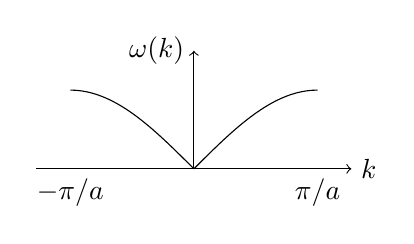
\begin{tikzpicture}
      \draw[->] (-2,0) -- (2,0) node[right] {$k$};
      \draw[->] (0,0) -- (0,1.5) node[left] {$\omega(k)$};
      \draw[domain=0:1.57,smooth,variable=\x,black] plot ({\x},{sin(deg(\x))});
      \draw[domain=-1.57:0,smooth,variable=\x,black] plot ({\x},{-sin(deg(\x))});
      \draw (1.57,0) node[below]{$\pi/a$};
      \draw (-1.57,0) node[below]{$-\pi/a$};
\end{tikzpicture}
\end{center}
The `first Brillouin Zone (BZ)" refers to the range of $q$-vectors that describe the displacements of the masses such that the phase difference between adjacent masses in part (i) is no bigger than $\pi$. Nyquist's criterion states that, because of aliasing, waves with $q$-vectors such that phase differences between adjacent masses with moduli greater than $\pi$ have displacement patterns equivalent to those with $q$-vectors equal to $q-\frac{n\pi}{a}$. Therefore, it is conventional to only consider the range $q\in[-\pi/a,\pi/a)$. Other BZ will contain the same information, as long as, the difference between the end points is equal to an integer number of reciprocal lattice vectors, $\frac{n\pi}{a}$ for $n\in\mathbb{Z}$. 
\item Each unit cell contains two masses $m$ and $M$. We label such that even index $n=2p$ has mass $m$ while the odd index $n=2p+1$ has mass $M$. The corresponding equations of motion are
$$m\ddot{u}_{2p}=-\alpha(u_{2p}-u_{2p+1})-\alpha(u_{2p}-u_{2p-1})$$
$$M\ddot{u}_{2p+1}=-\alpha(u_{2p+1}-u_{2p+2})-\alpha(u_{2p+1}-u_{2p})$$
We seek solutions of the form $u_{2p}=Xe^{i(\omega t-q2pa)}$ and $u_{2p+1}=Ye^{i(\omega t-q(2p+1)a}$. Substitute them and matriculate the resultant coupled equations:
$$\begin{pmatrix}-m\omega^2&0\\0&-M\omega^2\\\end{pmatrix}\begin{pmatrix}X\\Y\\\end{pmatrix}=-2\alpha\begin{pmatrix}1&-\cos(qa)\\-\cos(qa)&1\\\end{pmatrix}\begin{pmatrix}X\\Y\\\end{pmatrix}$$
Solving this gives
$$\omega^2=\frac{\alpha}{mM}\bigg[m+M\pm\sqrt{(m+M)^2-4mM\sin^2qa}\bigg]$$
The BZ is now modified to have $q\in[-\frac{\pi}{2a},\frac{\pi}{2a})$ since the real space periodicity is doubled. The dispersion relation have two branches: the higher branch corresponds to neighbouring atoms being between $\frac{\pi}{2}$ and $\pi$ out of phase, and it is called the optical branch, while the lower branch corresponds to neighbouring atoms being between $0$ and $\frac{\pi}{2}$ out of phase with each other, and this is called the acoustic branch. Whenever $q=\frac{n\pi}{2a}$, the gradient $v_s=\frac{\partial\omega}{\partial q}$ must be zero as it corresponds to standing waves.
\item The dispersion relation is as follow, where the optical and acoustic branches are in red and blue respectively:
\begin{center}
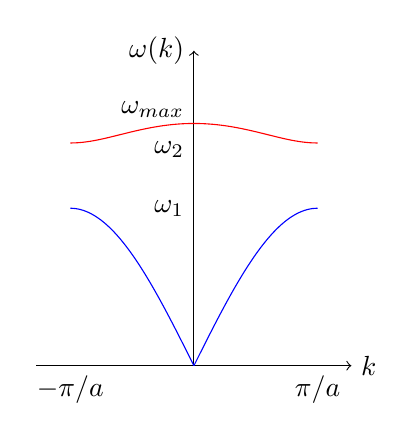
\begin{tikzpicture}
      \draw[->] (-2,0) -- (2,0) node[right] {$k$};
      \draw[->] (0,0) -- (0,4) node[left] {$\omega(k)$};
      \draw[domain=0:1.57,smooth,variable=\x,red] plot ({\x},{2*sqrt(0.5*(1+2+sqrt((1-2)^2+2*(cos(deg(\x))^2))))});
      \draw[domain=-1.57:0,smooth,variable=\x,red] plot ({\x},{2*sqrt(0.5*(1+2+sqrt((1-2)^2+2*(cos(deg(\x))^2))))});
      \draw[domain=-1.57:0,smooth,variable=\x,blue] plot ({\x},{-2*sin(deg(\x))});
      \draw[domain=0:1.57,smooth,variable=\x,blue] plot ({\x},{2*sin(deg(\x))});
      \draw (0,2) node[left]{$\omega_1$};
      \draw (0,2.75) node[left]{$\omega_2$};
      \draw (0,3.25) node[left]{$\omega_{max}$};
      \draw (1.57,0) node[below]{$\pi/a$};
      \draw (-1.57,0) node[below]{$-\pi/a$};
\end{tikzpicture}
\end{center}
The labelled $\omega$ quantities are
$$\omega_{max}=\sqrt{\frac{2\alpha(m+M)}{Mm}},\quad\omega_1=\sqrt{\frac{2\alpha}{M}},~\omega_2=\sqrt{\frac{2\alpha}{m}}$$
Hence, the gap at the edge of the first BZ is
$$\Delta\omega=\sqrt{\frac{2\alpha}{m}}-\sqrt{\frac{2\alpha}{M}}$$
\item The dispersion relation would depend on the direction as well, i.e. $\mathbf{q}$ and not $|\mathbf{q}|$. It would be very complicated, depending on what crystal structure was used. $\omega(\mathbf{q})$ will have two answers for each $\mathbf{q}$ and the gradients will be zero at the zone boundary and at the edges, but there may well be interior points other than origin at which $\frac{\partial\omega}{\partial\mathbf{q}}=0$ as well.
\end{enumerate}
\end{ans}
\subsubsection{Section D}
\begin{qns}[CMP Essay]
Explain the key principles and approximations underlying the Debye theory of heat capacity in solids. In particular, show why the heat capacity according to this theory is proportional to $T^3$ at low temperature.\hfill\textbf{[20]}
\end{qns}
\begin{ans}
In the Debye model, we assume the lattice vibrations are waves with speed $v_s$, speed of sound in the solid, i.e. for all wavelengths, $\omega=v_sq$, where $q$ is the wavevector of the lattice vibration. We compute the density of states of lattice vibrations in 3D as a function of $q$:\\[5pt]
The allowed states form a regular lattice of points in the positive octant of $k$-space. Each state occupies a volume of $\pi^3/V$. We consider the states within a shell of width $dk$, at radius $k$. The number of states in the shell is the volume of the shell divided by the volume of one state.
$$dN=g(k)dk=\frac{3(4\pi k^2/8)dk}{\pi^3/V}=\implies g(k)=\frac{3Vk^2}{2\pi^2}$$
where we included a factor of 3 to allow for 2 transverse modes and 1 longitudinal mode. Hence,
$$g(q)dq=\frac{4\pi q^2dq}{(2\pi/L)^3}3\implies g(\omega)d\omega=\frac{3V\omega^2d\omega}{2\pi^2v_s^3}$$
such that $\int_0^{\omega_D}g(\omega)d\omega=3N$ where $\omega_D$ the cutoff frequency (Debye frequency) is imposed to have a finite number of modes. We then have $\omega_D^3V=6N\pi^2v_s^3$ and hence rewriting $g(\omega)d\omega=\frac{9N\omega^2d\omega}{\omega_D^3}$. We can thus define a Debye temperature $\Theta_D=\hbar\omega_D/k$. Let $\beta=1/k_BT$, the internal energy is 
$$U=\int_0^{\omega_D}g(\omega)\hbar\omega(0.5+(e^{\beta\hbar\omega}-1)^{-1})d\omega=\frac{9}{8}N\hbar\omega_D+\frac{9N\hbar}{\omega_D^3}\int_0^{\omega_D}\frac{\omega^3d\omega}{e^{\hbar\omega\beta}-1}$$
The heat capacity per mole will be $\frac{9R}{x_D^3}\int_0^{x_D}\frac{x^4e^xdx}{(e^x-1)^2}$ where $x_D=\hbar\omega_D/k_BT$. At high temperature $C\rightarrow\frac{9R}{x_D^3}\int_0^{x_D}\frac{x^4}{x^2}dx=3R$ as expected. At low temperatures, $C\rightarrow\frac{9R}{x_D^3}\int_0^\infty\frac{x^4e^xdx}{(e^x-1)^2}=\frac{12R\pi^4}{5x_D^3}$, hence proportional to $T^3$. This is the phononic contribution to the heat capacity.\\[5pt]
In general, both electrons and phonons contribute to heat capacity. We note that the phononic contributions completely dominate the specific heat at high temperatures. Well below the room temperature, their contribution falls off as $T^3$ (Debye's theory), and at very low temperatures it drops below the electronic contribution, which only decreases linearly with $T$ (electronic contribution dominates now), i.e. 
$$C_V=\gamma T+AT^3$$
where $\gamma\approx 1.67$ (in theory) and $A$ are constants. We note that there may be some discrepancy between theory and experiment due to electrons moving with an effective mass (due to the periodic lattice)
\end{ans}
\newpage
\begin{qns}[OWO Short Notes]
Write brief notes on two of the following:\hfill\textbf{[20]}
\begin{itemize}
    \item Fresnel diffraction from circular structures;
    \item the Fabry-Pérot interferometer;
    \item diffraction patterns from diffraction gratings.
\end{itemize}
\end{qns}
\begin{ans}\leavevmode
\subsubsection*{Fresnel diffraction from circular structures:}
Consider a spherical source with strength $a_S$, at distance $s(x,y)$ from the aperture element $dxdy$ (with overall aperture function $h(x,y)$, then the total amplitude at point P, at a distance $r$ from the aperture element, is
$$\psi_P=-\int\frac{i}{\lambda}h(x,y)K(\theta)\frac{a_Se^{ik(s+r)}}{sr}dxdy$$
where $K(\theta)$ is the obliquity factor. This is the Fresnel-Kirchhoff diffraction integral, which is valid in the limit of distances greater than the wavelength of light, allowing us to neglect the vector nature of the electromagnetic wave. In the case of Fresnel diffraction (diffracted beam on-axis), we assume further that
\begin{itemize}
    \item the angles to the edge of the aperture are small enough that we can neglect the obliquity factor, and thus take $K(\theta)=1$;
    \item that the variations in $r_1$ and $r_2$ over the aperture are negligible as far as the denominator is concerned: $r_1\sim a$ and $r_2\sim b$ but note variations in $(r_1+r_2-a-b)$ are not negligible compared with $\lambda$ and so have a significant effect on the phase term.
\end{itemize}
Under these approximations, we have $\psi_P(0,0)$ to be directly proportional to
$$\int_\Sigma h(x,y)e^{ik(x^2+y^2)/2R}dxdy$$
where the path from S to P via the aperture element at $(x,y)$ is
$$r_1+r_2\approx a+b+\frac{x^2+y^2}{2a}+\frac{x^2+y^2}{2b}$$
Writing $\frac{1}{R}=\frac{1}{a}+\frac{1}{b}$, we have the optical path to be directly proportional to $(x^2+y^2)/2R$. Here, the quadratic phase in the diffraction integral can't be ignored since the distances between the screen and the aperture is of order $D^2/\lambda$ or smaller, where $D$ is the maximum dimension of the aperture.\\[5pt]
Consider a circular aperture of radius $r_a$. The obliquity factor, as well as, the variation in $r_1$ and $r_2$ across the aperture are retained. We only consider the pattern on-axis. Dividing the aperture elements of radius $\rho$ and thickness $d\rho$, we have the diffraction integral to be
$$\int_{\rho=0}^{\rho=r_a}\frac{K}{(a^2+\rho^2)^{0.5}(b^2+\rho^2)^{0.5}}e^{0.5ik\rho^2/R}2\pi\rho d\rho=\int_{s=0}^{s=r_a^2}\frac{K(s)}{(a^2+s)^{0.5}(b^2+s)^{0.5}}e^{i\pi s/(\lambda R)}\pi ds$$
The integral can be evaluated graphically using the phasor diagram. The phase $\phi=\frac{\pi s}{\lambda R}$ varies linearly with $s$, and the elemental contributions to the integral are approximately $ds$, so as $s$ increases the phasor diagram is approximately a circle. The term before the exponential is a slowly decreasing function of $s$ (denominator obviously increases with $s$, and $K$ decreases with $s$), thus the radius of the circle in the phasor diagram gradually decreases with $s$. To calculate the diffracted amplitude, consider the spanning vector from point O to the point a distance $s$ along the curve. The curve spirals inwards, so in the absence of an obstruction or aperture, the integration range is from O to F, corresponding to $s=\infty$. OF is thus the amplitude of the unobstructed wavefront.
\begin{figure}[H]
    \centering
    \includegraphics[width=\linewidth]{fresnelcircular.PNG}
    \caption{Left: Fresnel Diagram for Circular aperture. Top Right: Fresnel half period zones. Bottom Right: Phasor Diagram for a central obstacle.}
\end{figure}
In the circular geometry, these are concentric circular zones in the aperture plane, over which the phase at the observation point changes by $\pi$. We define the first zone as the circular region in the aperture plane which satisfies $0\leq\phi(\rho)\leq\pi$, which corresponds to $\rho^2\leq\lambda R$. The $n$th zone corresponds to the annulus satisfying $(n-1)\pi\leq\phi(\rho)\leq n\pi\implies\sqrt{(n-1)\lambda R}\leq\rho\leq\sqrt{n\lambda R}$. Note that the area of each zone is the same, in the quadratic approximation:
$$\pi(\rho_n^2-\rho_{n-1}^2)=\pi\lambda R$$
If we neglect the obliquity factor and the variation of $r_1$ and $r_2$, each zone would contribute equally to the amplitude at P. The phasor diagram would be circular. Odd numbered zones add to, and even numbered zones subtract from the overall amplitude at P. So on the optic axis of a circular aperture of radius $r_a$, the aperture includes $N$ zones, given by $r_a^2=N\lambda R$.\\[5pt]
If $N$ is odd, we get a bright spot at P, $\psi\sim2\psi_u$ (unobstructed). If $N$ is even, we get a dark spot at P, hence $\psi\sim 0$. For large apertures, the small angle approximations begin to break down. The spiralling in effect in the phasor diagram due to the $1/r$ terms in the diffraction integral becomes noticeable. This effect is further enhanced since $K(s)<1$. The width of the outer zones also increases, as the higher-order terms become important.\\[5pt]
Consider a circular obstruction on the axis. For an obstacle of radius $r_a$, the inner zones up to $\rho=r_a$ are obscured, but all the outer zones are clear. The limits of integration for the diffraction integral are $\rho=r_a$ to $\rho=\infty$. The relevant spanning vector in the phasor diagram is from F to A, which spans an arc angle of $\phi_a=\frac{\pi r_a^2}{\lambda R}$.\\[5pt]
Provided that $r_a$ is not too large, the intensity is therefore close to that expected in the absence of any obstruction. This leads to a bright spot on the axis, known as Poisson's spot. Close to the obstruction, the diffracted angles become large so that $K$ falls, and no spot is observable.
\newpage
\subsubsection*{The Fabry-Pérot interferometer:}
Consider a film of air (of thickness $d$) sandwiched between two mirrors, known as a Fabry-Pérot etalon. A fraction $t$ of this beam is transmitted in passing from glass to air, and a further fraction $t'$ transmitted in passing from air to glass, giving an emerging beam of amplitude $tt'=T$. This etalon produces a fringe pattern with much sharper features than a simple thin film, and is useful for high resolution spectroscopy. \\[5pt]
Each successive beam emerging from the etalon acquires a factor of $R:=r^2$ in amplitude and a phase shift $\delta$, where $\delta=\frac{4\pi d}{\lambda}\cos\theta$ (thin film). The total intensity transmission of the etalon is $|A|^2$ where $A=Te^{i\omega t}\sum_{n=0}^\infty R^ne^{-in\delta}$:
$$\frac{Te^{i\omega t}}{1-Re^{-i\delta}}\frac{Te^{-i\omega t}}{1-Re^{i\delta}}=\bigg|\frac{T}{1-Re^{i\delta}}\bigg|^2=\frac{T^2}{(1-R\cos\delta)^2+R^2\sin^2\delta}=\frac{T^2}{(1-R)^2}\bigg(\frac{1}{1+(4R/(1-R)^2))\sin^2(\delta/2)}\bigg)$$
The fringe pattern has maxima at $\delta=\frac{4\pi d}{\lambda}\cos\theta=2m\pi$ for $m\in\mathbb{Z}^+$. At normal incidence $\theta=0$ we have an integer number of half wavelengths between the mirrors.\\[5pt]
Although a Fabry-Pérot etalon will in general produce narrow and sharply defined circular fringes (of constant inclination $\theta$), in practice use them at normal incidence and detect the transmitted intensity at angles very close to $\theta=0$. By varying the spacing of the mirrors and using a photodiode to measure the transmitted intensity it is possible to measure the spectrum of the incident light, with each wavelength component producing its own set of peaks as a function of $d$.\\[5pt]
In practice, one cannot sum the geometric series to infinity above as it assumes that the etalon is infinite in extent (and that the plates are perfectly parallel, with uniform reflectivites), and so we have a finite total path difference, which will blur this resolution.
\begin{figure}[H]
    \centering
    \includegraphics[width=\linewidth]{fabryperot.PNG}
    \caption{(Top Left) Geometry of Fabry Pérot Etalon. (Top Right) Free Spectral Range and Resolution of Fabry Pérot Etalon. (Bottom Left) Intensity Profile of Fabry Pérot Etalon. (Bottom Right) Finesse Profile of Fabry Pérot Etalon.}
\end{figure}
The sharpness of the peaks is a function of $\delta$. The maximum value of $\frac{I_{out}}{I_{in}}=\frac{T^2}{(1-R)^2}$ where $\delta=2m\pi$. We define the half-width of the peaks $\delta_{1/2}$ as the change in $\delta$ required for the intensity to reduce to half its maximum value.
$$\frac{4R}{(1-R)^2}\sin^2(0.5\delta_{1/2})=1\implies\delta_{1/2}\approx\frac{1-R}{\sqrt{R}}$$
It is useful to define the finesse, $\mathcal{F}$ as the ratio of separation of successive peaks in $\delta$ (equal to $2\pi$) to their full-width at half maximum $(2\delta_{1/2})$
$$\mathcal{F}=\frac{2\pi}{2\delta_{1/2}}=\frac{\pi\sqrt{R}}{1-R}$$
The finesse is a measure of the quality of the etalon and becomes high as $R\rightarrow 1$. The chromatic resolving power of the etalon is defined as $\frac{\lambda}{\Delta\lambda}$.
$$d\delta=-\frac{4\pi d\cos\theta}{\lambda^2}d\lambda\implies|d\delta|:=\Delta\delta=\frac{\delta}{\lambda}\Delta\lambda=2\delta_{1/2}\implies\frac{\lambda}{\Delta\lambda}=\frac{2\pi d\cos\theta}{\lambda\delta_{1/2}}$$
Since $2d\cos\theta=m\lambda$ at maxima, the resolving power, is $\frac{\lambda}{\Delta\lambda}=\frac{m\pi}{\delta_{1/2}}=m\mathcal{F}$. This has the same form as the resolving power in the $m$th order for a diffraction grating of $N$ lines, where $N_{eff}$ is $\mathcal{F}$ of the Fabry-Pérot interferometer. This effective number is also the number of interfering beams in the interferometer.\\[5pt]
If $R=0.95$, $d=5$ mm, $\lambda=500$ nm, the resolving power is more than $10^6$ comparable with a grating spectrometer with a very large grating. Unfortunately, neighbouring orders with different wavelengths will overlap. The wavelength difference at which this  overlapping takes place is known as the free spectral range. At normal incidence, the maxima is at $2d=m\lambda\implies-\frac{2d}{\lambda^2}d\lambda=dm$. When $m$ is large, we can use this to find the wavelength change $(\Delta\lambda)_{fsr}$ corresponding to $\Delta m=1$, i.e.
$$1=\Delta m\frac{2d}{\lambda^2}(\Delta\lambda)_{fsr}=\frac{m}{\lambda}(\Delta\lambda)_{fsr}$$
The free spectral range $(\Delta\lambda)_{fsr}=\frac{\lambda}{m}$. The free spectral range around $\lambda=500$ nm is only 0.025 nm. Etalons are more suitable for measuring the fine structure of narrow spectral lines. The number of resolution elements across the spectrum is $\frac{(\Delta\lambda)_{fsr}}{(\Delta\lambda)_{res}}=\mathcal{F}$.
\subsubsection*{Diffraction patterns from diffraction gratings:}
Consider the diffraction pattern in a plane at a distance $L$ from the aperture. We denote the coordinates of point P in this plane by $(x_0,y_0)$ and further assume P to be close to the axis. Assume that the source S is a large distance behind the aperture, and the aperture is illuminated with a plane wave at normal incidence. The wave amplitude at P is directly proportional to the Fraunhofer integral
$$\int_\Sigma\psi_\Sigma h(x,y)e^{-ik(x_0x+y_0y)/R}dxdy$$
Moreover, the condition for Fraunhofer diffraction is $\frac{k(x^2+y^2)}{2R}<<\pi$. The Fraunhofer integral is a simplified version of the general Fresnel-Kirchhoff diffraction integral, where the approximation $x_0/L,y_0/L<<1$ gives a linear phase variation (as seen from any given point on the aperture plane). We see that the Fraunhofer integral is actually a Fourier transform of the aperture function $h(x,y)$. This Fourier transform relates real space variables $x,y$ to the conjugate ones $q=k\sin\theta$ and $p=k\sin\xi$. For some one-dimensional simple apertures, we can easily obtain the analytic descriptions of the Fraunhofer diffraction patterns:
$$\mathcal{F}[\sum_{m=0}^\infty\delta(y-mD)]=\sum_{m=0}^\infty\delta(q-m\frac{2\pi}{D})$$
$$\mathcal{F}[\text{rect}(y/a)]=a\sinc(qa/2)$$
These two functions are key building blocks in deriving the diffraction pattern of more complicated aperture functions. To do this, we need the convolution theorem. Convolution theorem states that the Fourier transform of a product of two functions is the convolution of the Fourier transforms of the individual functions.
$$f(y)*g(y)=\int_{-\infty}^\infty f(u)g(y-u)du$$
This is illustrated below.
\begin{figure}[H]
    \centering
    \includegraphics[scale=0.75]{convolution.PNG}
\end{figure}
For a diffraction grating of finite span of slits with finite widths, $h(x)$ is given by
$$h(x)=\bigg(\sum_{m=0}^\infty\delta(y-mD)*\text{rect}\frac{y}{a}\bigg)\times\text{rect}\frac{y}{b}$$
which is a convolution of a single slit top-hat function $\text{rect}\frac{y}{a}$ and an infinite span delta comb with separation intervals equal to the spacing between the slits, $D$, followed by a multiplication of another top-hat function to ensure the grating is finite. Surely, $b>a$, where $a$ is the width of each slit and $b$ is the length span of the grating. By the Convolution theorem, the Fourier transform of the aperture function is 
$$\mathcal{F}[h(x)]=\bigg(\sum_{m=0}^\infty\delta(q-m\frac{2\pi}{D})\times a\sinc\frac{qa}{2}\bigg)*b\sinc\frac{qb}{2}$$
The corresponding diffraction pattern is a sinc envelope (dependent on the width of each slit, $a$) and sinc peaks (dependent on the length span of the grating, $b$) separated by $\frac{2\pi}{D}$ in $q$-space, hence related to the slit separation $D$. Hence
\begin{enumerate}[label=(\alph*)]
    \item The spacing between the grating lines $D$ is inversely proportional to the separation between intensity peaks, $\frac{2\pi}{D}$;
    \item The width of the individual peaks is inversely proportional to the overall extent of the grating $b$.
    \item The amplitude distribution over an individual line is dependent on the wider sinc envelope, in turn affected by the width of each slit $a$. Changing the amplitude distribution over an individual line would involve the Fourier transform of the function $g(x)$ that represents this amplitude distribution over this individual line. 
    \item Varying the phase distribution over an individual line would involve translating the pattern of that corresponding line linearly, by an amount equal to this new phase shift.
\end{enumerate}
\end{ans}
\newpage
\section{2014}
\subsection{Paper 1}
\subsubsection{Section A}
\begin{qns}[Identical Particles]
Consider a system of nine electrons in a 3D Coulomb potential. Assuming that the electrons do not interact with one another, calculate the ratio of the energy of the first excited state to that of the ground state.\hfill\textbf{[4]}
\end{qns}
\begin{ans}
The Hamiltonian is highly degenerate, with energies $E_n\propto -\frac{1}{n^2}$, where $n$ is the quantum number of the state. For the ground state of this nin-electron system, we need to fill the lowest nine single particle states:
\begin{itemize}
    \item 1s: 2 electrons fill here;
    \item 2s: 2 electrons fill here;
    \item 2p: 5 out of 6 states are filled.
\end{itemize}
But the 2s and 2p orbitals are degenerate states, with the same energy. For the first excited state, one of the outermost shell electron (which is the one in the 2p orbital) has to be promoted to the next higher energy orbital (which is the 3s orbital). Thus the ratio of the energy of the first excited state to that of the ground state is
$$\frac{(2/1)+(6/4)+(1/9)}{(2/1)+(7/4)}=\frac{26}{27}$$
\end{ans}
\begin{qns}[1D Potential]
Draw an annotated sketch of the wavefunctions of the three lowest energy eigenstates in a quantum-mechanical, 1D, square well of finite depth, assuming that all three states are bound states.\hfill\textbf{[4]}
\end{qns}
\begin{ans}
The sketches are a slight variation from that of the infinite potential well. The difference is, it does not terminate ($\psi=0$) at the edges, but rather it is a point of inflexion there (transition between classically allowed and classically forbidden region). Outside of the well, the wavefunction is an exponential decay. Other features to ensure you note (assuming centre of well is at $x = 0$):
\begin{itemize}
    \item All states must be in an eigenstate of parity, i.e. symmetric about the centre of the well;
    \item Both $\psi$ and $\frac{d\psi}{dx}$ are continuous everywhere, especially at the edges.
    \item The ground state is even, has no nodes, is exponential in the classically forbidden regions, cosine in the classically allowed.
    \item The first excited state is odd, shorter wavelength in the well, slower decay outside
    \item The second excited state is even, even shorter wavelength inside, even slower decay outside.
\end{itemize}
\end{ans}
\begin{qns}[Misc]
Using Heisenberg’s uncertainty principle, estimate how many collisions per second an $\alpha$-particle would have with the walls of a nuclear potential well of size $10^{-14}$ m.\hfill\textbf{[4]}
\end{qns}
\begin{ans}
The Heisenberg's Uncertainty Principle states $\Delta p\Delta x\geq\frac{\hbar}{2}$. We estimate $\langle v\rangle\sim\Delta v$. Then the frequency of collisions is
$$\frac{\langle v\rangle}{\Delta x}=\frac{\hbar}{2m_\alpha(\Delta x)^2}=\frac{(6.626\times10^{-34}/2\pi)}{2(1.67\times10^{-27}\times 4)(10^{-14})^2}=7.9\times10^{19}Hz$$
\end{ans}
\newpage
\begin{qns}[Probability and Distribution]
A beam of particles is incident on a detector. The particles are in three energy ranges, labelled Low, Medium, and High; the proportions are 65, 30, and 5\% respectively. Due to electronic dead time, there is a probability that a particle in each energy range is not detected, given by 5, 20, and 50\%, respectively. Using Bayes’ theorem, find the probability that a detected particle is in the High energy range.\hfill\textbf{[4]}
\end{qns}
\begin{ans}
We are given the conditional probability of being detected given High, Low and Medium respectively to be $1-0.5=0.5$, $1-0.05=0.95$, $1-0.2=0.8$. The probability of being High, Low and Medium respectively are $0.05$, $0.65$ and 0.3. Using Bayes' Theorem,
$$P(High|Detected)=\frac{P(Detected|High)P(High)}{\sum_{i=Low,Medium,High}P(Detected|i)P(i)}=\frac{0.5\times 0.05}{0.5\times0.05+0.8\times0.3+0.95\times0.65}$$
which is $\frac{10}{353}$.
\end{ans}
\begin{qns}[Probability and Distribution]
During an experiment, it is found that temperature measurements follow a Gaussian distribution with mean 273 K and r.m.s. 10 K. Using the graph of $y(x)=\frac{1}{\sqrt{2\pi}}\int_{-\infty}^xe^{-t^2/2}dt$ drawn below, estimate the probability that a particular measurement exceeds 293 K.\hfill\textbf{[4]}
\begin{figure}[H]
    \centering
    \includegraphics[scale=0.75]{2014P1A5Q.PNG}
\end{figure}
\end{qns}
\begin{ans}
The Gaussian distribution have parameters $\mu=273$ and $\sigma=10$, then the standard normal variable is $Z=\frac{X-\mu}{\sigma}=\frac{293-273}{10}=2$. Hence, reading off from the graph: $1-y(2)=1-0.975=0.025$.
\end{ans}
\newpage
\subsubsection{Section B}
\begin{qns}[1D Potential]
A quantum-mechanical particle of mass $m$ and energy $E$ is incident on a potential barrier of the form 
$$V(x)=
\left\{
        \begin{array}{ll}
      0 & x<0 \\
      U & x\geq0
        \end{array}
    \right.$$
\begin{enumerate}[label=(\roman*)]
\item For $E < U$, show that the particle is totally reflected with phase $\delta=-2\cos^{-1}\sqrt{\frac{E}{U}}$.\hfill\textbf{[7]}
\item Find the wavefunction in the region $x > 0$ and explain how it can be non-zero even though the particle is totally reflected.\hfill\textbf{[3]}
\item Suppose now the potential is modified such that $V(x) = 0$, for $x > a$ (where $a > 0$). Show that, when $a$ is large, the transmission probability depends exponentially on $a$ and find the form of the exponent.\hfill\textbf{[5]}
\item Find the condition for the approximation of large $a$ to be a good one.\hfill\textbf{[2]}
\item Estimate the transmission probability for an electron with energy 50 meV tunnelling through a barrier of height 200 meV and width 10 nm.\hfill\textbf{[3]}
\end{enumerate}
\end{qns}
\begin{ans}\leavevmode
\begin{enumerate}[label=(\roman*)]
\item The Schrodinger equation for $x<0$ is $\psi''=-\frac{2mE}{\hbar^2}\psi<0$ and so $\psi=c_2(1+r)e^{-ikx}$, where $\frac{\hbar^2k^2}{2m}=E$. For $x\geq0$, $\psi''=\frac{2m}{\hbar^2}(U-E)\psi>0$ would have $\psi=c_1e^{qx}+c_2\tau e^{-qx}$ where $\frac{\hbar^2q^2}{2m}=U-E$. $\psi$ is normalizable, hence $c_1=0$. The boundary conditions are:
\begin{itemize}
    \item $\psi$ continuous at $x=0$: $1+r=\tau$;
    \item $\psi'$ is continuous at $x=0$: $ik(1-r)-q\tau$.
\end{itemize}
We thus have $r=\frac{1-i(q/k)}{1+i(q/k)}$. This is in the form of $\frac{z}{z^*}$, which obviously has modulus 1 and argument $\arg(z)-\arg(z^*)=\arg(z)+\arg(z)$. But, argument for $z=x+iy$ can also be written as $\cos^{-1}\frac{x}{\sqrt{x^2+y^2}}$. The phase is 
$$\delta=-\arg(r)=2\cos^{-1}\frac{1}{\sqrt{1+(q^2/k^2)}}=2\cos^{-1}\sqrt{\frac{E}{U}}$$
\item For $x>0$, $\psi=c_2\tau e^{-qx}$. Since it is a beam of particles, the wavefunction represents a stock of probability in the classically forbidden region.
\item To ensure normalization, when $a$ is very huge, $\psi$ is approximately zero outside of the barrier, and $\psi$ in the barrier is dominated by the term $e^{-qx}$. Thus, the transmission probability is $\propto e^{-qx}$.
\item For a good approximation, the transmission probability should be less than 0.01, and thus
$$a\geq-\frac{\ln(1/100)}{2\sqrt{2m(U-E)/\hbar^2}}=\hbar\frac{\ln(100)}{2}\frac{1}{\sqrt{2m(U-E)}}$$
\item The wavenumber in $x\geq 0$ is
$$q=\frac{\sqrt{2m(U-E)}}{\hbar}=\frac{\sqrt{2(9.11\times10^{-31})(200-50)\times10^{-3}\times 1.6\times10^{-19}}}{6.626\times10^{-34}/2\pi}=1.983\times10^9$$
and thus the transmission probability is proportional to $e^{-2qa}=e^{-2(1.983\times 10^9)(10\times10^{-9})}=e^{-39.659}=6\times10^{-18}$, which is very small.
\end{enumerate}
\end{ans}
\newpage
\begin{qns}[Central Potential]
The electron in a hydrogen atom satisfies the time-independent Schrödinger equation
$$-\frac{\hbar^2}{2m}\nabla^2\psi-\frac{e^2}{4\pi\epsilon_0r}\psi=E\psi$$
where the symbols have their usual meanings.
\begin{enumerate}[label=(\roman*)]
\item Explain how this equation may be solved by separation of variables with the trial solution
$$\psi_{nlm}=R_{nl}(r)Y_{lm}(\theta,\phi)$$
and explain the meaning of $n$, $l$, and $m$.\hfill\textbf{[4]}
\item Show that there exists a normalized solution of the form $\psi=A re^{-\alpha r}\cos\theta$ and find $A$, $\alpha$, $l$, and the energy eigenvalue.\hfill\textbf{[10]}
\item Explain why $\psi$ is an eigenstate of parity and find its eigenvalue.\hfill\textbf{[4]}
\item Explain how it is possible that the Hamiltonian is spherically symmetric, but that the eigenstate $\psi$ is not.\hfill\textbf{[2]}
\end{enumerate}
\end{qns}
\begin{ans}\leavevmode
\begin{enumerate}[label=(\roman*)]
\item We have $\nabla^2=\frac{1}{r^2}[\frac{\partial}{\partial r}(r^2\frac{\partial}{\partial r})+\frac{1}{\sin\theta}\frac{\partial}{\partial\theta}(\sin\theta\frac{\partial}{\partial\theta})+\frac{1}{\sin^2\theta}\frac{\partial^2}{\partial\phi^2}]$, then separation of variables will separate the solution such that both sides are equal to a constant:
$$\frac{1}{R_{nl}}\frac{d}{dr}\bigg(r^2\frac{dR_{nl}}{dr}\bigg)+\frac{2mr^2}{\hbar^2}\bigg(E+\frac{e^2}{4\pi\epsilon_0r}\bigg)=-\frac{1}{Y_{lm}\sin\theta}\frac{d}{d\theta}\bigg(\sin\theta\frac{dY_{lm}}{d\theta}\bigg)-\frac{1}{Y_{lm}\sin^2\theta}\frac{d^2Y_{lm}}{d\phi^2}$$
A similar procedure can separate $Y_{lm}$ into individual functions of $\theta$ and $\phi$. The constants $n$, $l(l+1)$ and $m_l$ are separation constants:
\begin{itemize}
    \item principle quantum number, $n$: total energy of particle;
    \item angular momentum quantum number, $l$: total angular momentum of system $\hbar\sqrt{l(l+1)}$;
    \item magnetic quantum number, $m_l$: component of total angular momentum along the $z$-axis $\hbar m_l$.
\end{itemize}
\item With $A\cos\theta\frac{1}{r^2}\frac{\partial}{\partial r}(r^2\frac{\partial re^{-\alpha r}}{\partial r})=A\cos\theta e^{-\alpha r}(\frac{2}{r}-4\alpha+\alpha^2r)$ and $Are^{-\alpha r}\frac{1}{r^2\sin\theta}\frac{d}{d\theta}(\sin\theta\frac{d}{d\theta}\cos\theta)=-2\frac{A}{r}e^{-\alpha r}\cos\theta$,
$$Ere^{-\alpha r}\cos\theta=-\frac{e^2}{4\pi\epsilon_0}e^{-\alpha r}\cos\theta-\frac{\hbar^2}{2m}\cos\theta e^{-\alpha r}\bigg[\frac{2}{r}-4\alpha+\alpha^2r-\frac{2}{r}\bigg]$$
which gives $\alpha=\frac{me^2}{8\pi\epsilon_0\hbar^2}:=\frac{1}{2a_0}$ and $E=-\frac{\hbar^2\alpha^2}{2m}=-\frac{\hbar^2}{8ma_0^2}$. Check normalization:
$$1=\int_0^\infty\int_0^\pi\int_0^{2\pi}|A|^2r^2e^{-2\alpha r}\cos\theta r^2d\phi d\theta dr=|A|^2\int_0^\infty r^4e^{-2\alpha r}dr\int_0^\pi \cos^2\theta\int_0^{2\pi}d\phi$$
which gives $|A|^2\frac{4!}{(2\alpha)5}\frac{-1}{3}[\cos^3\theta]_0^\pi 2\pi=1\implies|A|=\frac{1}{\sqrt{32\pi a_0^5}}$.
\item The parity operator inverts space through the origin. $\psi$ is an eigenstate of the parity operator with eigenvalue $-1$, i.e. odd symmetry:
$$\psi(r,\pi-\theta,\phi+\pi)=Are^{-\alpha r}\cos(\pi-\theta)=-Are^{-\alpha r}\cos\theta=-\psi$$
\item In general, if an operator $\hat{A}$ has a degenerate subspace, then all we can say that another operator $\hat{B}$ rotates within that degenerate subspace and nothing can be said whether $\hat{A}$ or $\hat{B}$ commutes. The Hamiltonian is spherically symmetric and thus commutes with any linear combinations of the generators of rotations $\{\hat{L}_x,\hat{L}_y,\hat{L}_z\}$. But this does not mean they have to share an eigenspace, since the Hamiltonian has degenerate eigenvalues.
\end{enumerate}
\end{ans}
\newpage
\begin{qns}[Angular Momentum]\leavevmode
\begin{enumerate}[label=(\roman*)]
\item Write down the commutation relations of the angular momentum operators $\hat{L}_x$, $\hat{L}_y$, and $\hat{L}_z$ and show that $\hat{L}_z$ commutes with $\hat{L}^2=\hat{L}_x^2+\hat{L}_y^2+\hat{L}_z^2$.\hfill\textbf{[4]}
\item Write down the eigenvalues of $\hat{L}^2$ and $\hat{L}_z$.\hfill\textbf{[2]}
\item The Hamiltonian of an asymmetric spinning top is given by
$$\hat{H}=a_x\hat{L}_x^2+a_y\hat{L}_y^2+a_z\hat{L}_z^2$$
where $a_x$, $a_y$ and $a_z$ are constants. Show that $[\hat{H},\hat{L}^2] = 0$ and comment on the implications for the eigenstates of $\hat{H}$.\hfill\textbf{[3]}
\item Letting $\hat{L}_\pm=\hat{L}_x\pm i\hat{L}_y$, show that $\hat{H}$ can be written as
$$\hat{H}=\alpha(\hat{L}_+^2+\hat{L}_-^2)+\beta(\hat{L}^2-\hat{L}_z^2)+\gamma\hat{L}_z^2$$
and find expressions for $\alpha$, $\beta$ and $\gamma$ in terms of $a_x$, $a_y$ and $a_z$.\hfill\textbf{[5]}
\item Using the relation
$$\hat{L}_\pm|l,m\rangle=\hbar\sqrt{l(l+1)-m(m\pm 1)}|l,m\pm 1\rangle$$
for the eigenstates $|l,m\rangle$ of $\hat{L}^2$ and $\hat{L}_z$, show that $|1,0\rangle$ is an eigenstate of $\hat{H}$ and find the energy eigenvalue.\hfill\textbf{[2]}
\item Find the other two eigenvalues corresponding to $l = 1$ and comment on how all three eigenvalues are related.\hfill\textbf{[4]}
\end{enumerate}
\end{qns}
\begin{ans}\leavevmode
\begin{enumerate}[label=(\roman*)]
\item $[\hat{L}_i,\hat{L}_j]=i\hbar\epsilon_{ijk}\hat{L}_k$ and $$[\hat{L}_z,\hat{L}^2]=[\hat{L}_z,\hat{L}_x^2]+[\hat{L}_z,\hat{L}_y^2]=[\hat{L}_z,\hat{L}_x]\hat{L}_x+[\hat{L}_z,\hat{L}_y]\hat{L}_y=\hat{L}_y\hat{L}_x-\hat{L}_x\hat{L}_y=0$$
\item $\hat{L}^2$: $\hbar^2l(l+1)$ and $\hat{L}_z$: $\hbar m_l$ with $-l\leq m_l\leq l$.
\item $[\hat{L}_x^2,\hat{L}^2]=\hat{L}_x[\hat{L}_x,\hat{L}^2]+[\hat{L}_x,\hat{L}^2]\hat{L}_x=0$. Similar for the other two terms, and so $[\hat{H},\hat{L}^2]=0$ which means that $\hat{L}^2$ and $\hat{H}$ share the same eigenbasis.
\item Expanding $\hat{L}_+^2+\hat{L}_-^2$ gives $2\hat{L}_x^2-2\hat{L}_y^2$, so
$$\hat{H}=2\alpha(\hat{L}_x^2-\hat{L}_y^2)+\beta(\hat{L}_x^2+\hat{L}_y^2)+\gamma\hat{L}_z^2$$
Comparing coefficients give $\alpha=\frac{a_x-a_y}{4}$, $\beta=\frac{a_x+a_y}{2}$ and $\gamma=a_z$.
\item The action of $\hat{H}$ on $|1,0\rangle$ is
$$\hat{H}|1,0\rangle=\frac{a_x+a_y}{2}2\hbar^2|1,0\rangle=\hbar^2(a_x+a_y)|1,0\rangle$$
where $\hat{L}_\pm|1,0\rangle=\sqrt{2}\hbar|1,\pm1\rangle$, $\hat{L}_+^2|1,0\rangle=\hat{L}_z|1,0\rangle=0$ and $\hat{L}^2|1,0\rangle=2\hbar^2$. Then, $|1,0\rangle$ is an eigenstate of $\hat{H}$ with energy eigenvalue $\hbar^2(a_x+a_y)$.
\item For $|l,m\rangle=|1,\pm1\rangle$, $\hat{L}_\mp|1,\pm1\rangle=\hbar\sqrt{2}|1,0\rangle$ and $\hat{L}_\mp^2|1,\pm1\rangle=|1,\mp1\rangle$. Then,
$$\hat{H}|1,\pm1\rangle=(\sqrt{2}\alpha\hbar)^2|1,\mp1\rangle+\beta\hbar^2|1,\pm1\rangle+\gamma\hbar^2|1,\pm1\rangle=2\hbar^2\frac{a_x-a_y}{4}|1,\mp1\rangle+\hbar^2\bigg(\frac{a_x+a_y}{2}+a_z\bigg)\hbar^2|1,\pm1\rangle$$
By inspection, we guess that $\frac{1}{\sqrt{2}}(|1,1\rangle\pm|1,-1\rangle)$ is an eigenstate. Indeed, it is and the eigenvalues are $(a_x+a_z)\hbar^2$ (+) and $(a_y+a_z)\hbar^2$ (-). The eigenvalues will become degenerate when the relative weights of the different angular momenta in the original Hamiltonian are the same, i.e. $a_x=a_y=a_z$.
\end{enumerate}
\end{ans}
\newpage
\begin{qns}[Harmonic Oscillator]\leavevmode
\begin{enumerate}[label=(\roman*)]
\item Write down the commutation relation for the operators $\hat{x}$ and $\hat{p}$ and show that $[f(\hat{x}),\hat{p}]=i\hbar f'(\hat{x})$, where $f$ is any function.\hfill\textbf{[3]}
\item Consider the Hamiltonian $\hat{H}=\frac{1}{2m}(\hat{p}+if(\hat{x}))(\hat{p}-if(\hat{x}))$. Show that this may be written as
$$\hat{H}=\frac{\hat{p}^2}{2m}+V(\hat{x})$$
and find $V(\hat{x})$.\hfill\textbf{[2]}
\item By considering $\int\psi^*\hat{H}\psi dx$, show that the energy eigenvalues are non-negative.\hfill\textbf{[3]}
\item The ground state, $\psi_0$, has vanishing energy. Show that it satisfies the differential equation

\hfill\textbf{[2]}
$$\hbar\frac{d\psi_0}{dx}+f(x)\psi_0=0$$
\item Let $\psi_1=(\hat{p}+if(\hat{x}))\psi_0$. Show $\hat{H}\psi_1=\alpha\psi_0+\beta\psi_1$ and find expressions for $\alpha$ and $\beta$ in terms of $f$.\hfill\textbf{[4]}
\item If $f$ is a polynomial of degree $n$, show that $n$ must be odd for $\psi_0$ to be normalizable.\hfill\textbf{[3]}
\item By considering $f=kx$, derive the energies and wavefunctions of the ground state and first excited states of the simple harmonic oscillator, with Hamiltonian\hfill\textbf{[3]}
$$\hat{H}_{SHO}=\frac{\hat{p}^2}{2m}+\frac{1}{2}m\omega^2\hat{x}^2$$
\end{enumerate}
\end{qns}
\begin{ans}\leavevmode
\begin{enumerate}[label=(\roman*)]
\item $[\hat{x},\hat{p}]=i\hbar$. $[f(\hat{x}),\hat{p}]=-\frac{\hbar}{i}\frac{\partial f(\hat{x})}{\partial x}$.
\item Expanding the expression for $\hat{H}$ and note the result from part (i), we have
$$\hat{H}=\frac{\hat{p}^2}{2m}+\frac{i}{2m}[f(\hat{x}),\hat{p}]+\frac{f^2(\hat{x})}{2m}\implies V(\hat{x})=-\frac{\hbar}{2m}f'(\hat{x})+\frac{f^2(\hat{x})}{2m}$$
\item From the form of $\hat{H}$, observe that $\psi^*\hat{H}\psi=\psi^*(\hat{p}+if(\hat{x}))(\hat{p}-if(\hat{x}))\psi$ is a norm of the wavefunction $(\hat{p}-if(\hat{x}))\psi$. Since the norm must be positive-definite (and hence its integral), then $\int\psi^*\hat{H}\psi dx$ must also be positive finite.
\item Since $\psi_0$ has vanishing energy, $\langle\psi_0|\hat{H}|\psi_0\rangle=0$. We thus must have
$$(\hat{p}-if(\hat{x}))|\psi_0\rangle=0\implies\hbar\frac{d\psi_0}{dx}+f(x)\psi_0=0$$
\item Evaluate $\hat{H}\psi_1$:
$$\frac{1}{2m}(\hat{p}+if(\hat{x}))(\hat{p}-if(\hat{x}))(\hat{p}+if(\hat{x}))\psi_0=\frac{1}{2m}(\hat{p}+if(\hat{x}))[(\hat{p}+if(\hat{x}))(\hat{p}-if(\hat{x}))+2\hbar f']\psi_0=\frac{2\hbar}{2m}(\hat{p}+i f(\hat{x}))f'\psi_0$$
where we used the commutator $[\hat{p}+if,\hat{p}-if]=i[f,\hat{p}]-i[\hat{p},f]=-2\hbar f'$, and next we then use $[\hat{p}+if,f']=[\hat{p},f']=-i\hbar f''$ to get
$$\hat{H}\psi_1=\frac{\hbar}{m}[f'(\hat{p}+if)-i\hbar f'']\psi_0=\frac{\hbar}{m}f'\psi_1-\frac{i\hbar^2}{m}f''\psi_0$$
Thus, $\alpha=-\frac{i\hbar^2}{m}f''$ and $\beta=\frac{\hbar}{m}f'$.
\item From part (iv),
$$\frac{d\psi_0}{dx}=-\frac{f(x)}{\hbar}\psi_0\implies\psi_0\propto\exp\bigg(-\frac{1}{\hbar}\int^x\sum_{n=0}^Na_nt^ndt\bigg)=\exp\bigg(-\frac{1}{\hbar}\sum_{n=0}^N\frac{a_nx^{n+1}}{n+1}\bigg)$$
which diverges at either $x\rightarrow\pm\infty$ unless the highest power is even and hence $N$ is odd. We have assumed $a_N>0$.
\item $f=kx$, and so $\psi_0\propto e^{-0.5kx^2/\hbar}$. $\psi_1$ satisfy
$$\psi_1=\frac{\hbar}{i}\frac{\partial\psi_0}{\partial x}+ikx\psi_0=2ikx\psi_0$$
Notice that $\hat{H}=\hat{H}_{SHO}-\frac{1}{2}\hbar\omega$, where $\omega=\frac{kx}{m}$. Thus, both Hamiltonians will share the same eigenstates. Then from part (v):
$$\hat{H}\psi_0=0\implies\hat{H}_{SHO}\psi_0=\frac{1}{2}\hbar\omega\psi_0$$
$$\hat{H}\psi_1=\frac{\hbar k}{m}\psi_1\implies\hat{H}_{SHO}\psi_1=\frac{1}{2}\hbar\omega\psi_1+\hbar\omega\psi_1=\frac{3}{2}\hbar\omega\psi_1$$
\end{enumerate}
\end{ans}
\newpage
\subsubsection{Section C}
\begin{qns}[QM Essay]
Write an essay on the Planck distribution of black-body radiation, including a discussion of the harmonic oscillator and the probability distribution of vibrational states. You should include, as an example, a sketch of the radiated intensity per unit wavelength vs. wavelength for the cosmic microwave background radiation, whose temperature is 2.7 K.\hfill\textbf{[20]}
\end{qns}
\begin{ans}
In 1900, Planck postulated that light is quantized in packets of energy, known as photons. This was revolutionary and changed our understanding of physics. In quantum field theory, we quantize electromagnetic waves and realize photons are essentially a bunch of harmonic oscillators. Inspired by the classical case, we take the (quantum analogue) Hamiltonian of the harmonic oscillator to be
$$\hat{H}=\frac{1}{2m}\hat{p}^2+\frac{1}{2}m\omega^2\hat{x}^2,\quad \omega\in\mathbb{R},~m\in\mathbb{R}$$
The energy eigenvalues could be solved by either directly solving the Schr\"{o}dinger's equation or invoking the operator method. Either way, we will have
$$E_n=(n+0.5)\hbar\omega$$
A similar approach can be done for a diatomic molecule, where its vibrational motion is quantized such that we have discrete vibrational energy states with $E_n=(n+0.5)\hbar\sqrt{\alpha/\mu}$ where $\mu$ is the reduced mass of the diatomic molecule and $\alpha$ is the stiffness of the chemical bond. The average vibrational energy per molecule is
$$\langle E\rangle=\frac{1}{2}\hbar\omega+\frac{\sum_{n=1}^\infty n\hbar\omega e^{-n\hbar\omega\beta}}{\sum_{n=1}^\infty e^{-n\hbar\omega\beta}}=0.5\hbar\omega+\frac{\hbar\omega}{e^{\hbar\omega\beta}-1}$$
The resultant probability distribution of vibrational states would follow the Boltzmann distribution (see classical thermodynamics), i.e. the probability of a state with energy $E_n$ is
$$p_n=\frac{1}{Z}e^{-E_n/k_BT}$$
We return to the main topic of blackbody radiation. An idealized blackbody absorbs all of the incoming radiation. When the blackbody is in thermal equilibrium with its surroundings, it radiates as much energy as it absorbs. Hence, a blackbody is a perfect absorber and perfect emitter. The maximum intensity of this radiation depends on its frequency and on the temperature of the blackbody. Accounting for blackbody radiation has been a mystery for many decades in the 19th to 20th century. Classical attempts include
\begin{itemize}
\item (1894) Wien's formula empirically fits the high frequency data but fails in the low frequency regime: $u(f,T)=\alpha f^3e^{-\frac{\beta f}{T}}$
\item In 1900, Rayleigh focused on understanding the nature of the electromagnetic radiation inside the cavity (which was modelled as a perfect blackbody). He considered the radiation to consist of standing waves of temperature $T$ with nodes at the metallic surfaces. These standing waves are harmonic oscillations of a large number of electrons present in the walls of the cavity.\\[5pt]
When the cavity is in thermal equilibrium, the electromagnetic density inside the cavity is equal to the energy density of the charged particles in the walls of the cavity, The number of standing waves (modes) of the radiation in the frequency interval $f$ to $f+df$ is $N(f)=\frac{8\pi f^2}{c^3}$. The average energy of the oscillators present on the cavity walls can be determined using the equipartition theorem of classical thermodynamics, which is $kT$. Thus, the energy density per unit frequency (given by Rayleigh-Jeans formula) is $u(f,T)=\frac{8\pi f^2}{c^3}kT$. 
This fits well for low frequency regime but fails for high frequency, which diverges to infinity. Hence, this problem was termed as the ``ultraviolet catastrophe''.
\end{itemize}
In reality, the arguments put forth by both Wien and Rayleigh were erroneous simply because they assumed the energy exchange between radiation and matter is continuous. Using Planck's postulate where the energy is an integer multiple of $hf$ ($h$ is Planck's constant), the average energy for a quantized oscillator is thus
$$\big \langle E \big \rangle = \frac{\sum_{n=0}^{\infty} nhfe^{-\frac{nhf}{kT}}}{\sum_{n=0}^{\infty}e^{-\frac{nhf}{kT}}}=\frac{hf}{e^{\frac{hf}{kT}}-1}$$
Hence we obtained the Planck distribution:
$$u(f,T)=\frac{8\pi f^2}{c^3}\frac{hf}{e^{\frac{hf}{kT}}-1}$$
Planck's distribution gives an exact fit for the entire frequency distribution. The total energy density can be found by integrating over the whole spectrum,
$$
\int_{0}^{\infty}u(f,T)df=\frac{8\pi h}{c^3}\int_{0}^{\infty}\frac{f^3}{e^{\frac{hf}{kT}}-1}df=\frac{8\pi^5 k^4T^4}{15h^3c^3}=\frac{4}{c}\sigma T^4$$
where $\sigma = \frac{2\pi^5 k^4}{15h^3c^2}$, consistent with Stefan-Boltzmann's law. In this way, Planck's relation leads to a finite total energy density of the radiation emitted by a blackbody, hence avoiding the ultraviolet catastrophe.
In the limit of very low frequencies $hf<<kT$, 
$$
u(f,T)\approx\frac{8\pi f^2}{c^3}\frac{hf}{\frac{hf}{kT}}=\frac{8\pi f^2}{c^3}kT
$$
On the other hand, in the limit of very high frequencies $hf>>kT$, the denominator will become very small
$$
u(f,T)=\frac{8\pi f^2}{c^3}\frac{hfe^{-\frac{hf}{kT}}}{1-e^{-\frac{hf}{kT}}}\approx\frac{8\pi hf^3}{c^3}e^{-\frac{hf}{kT}}$$
We can find the peak wavelength using Wien's Displacement Law, which relates the peak wavelength $\lambda_{max}$ of the radiation emitted by a black body of temperature $T$.
$$\lambda_{max}=\frac{2898.9\times 10^{-6}}{T}$$
The Wien's Distribution (black curve) do agree with Planck's Distribution for low frequencies ($f\rightarrow 0$) whereas the Rayleigh-Jeans' Distribution (blue curve)do agree with Planck's Distribution for high frequencies ($f\rightarrow\infty$). The Wien's Law helps us to determine the frequency where the energy density per unit frequency peaks at, given a constant temperature $T$.
\begin{center}
\begin{tikzpicture}
      \draw[->] (0,0) -- (8,0) node[right] {$f$};
      \draw[->] (0,-1) -- (0,3) node[left] {$u(f,T)$};
      \draw[domain=0:1.5,smooth,variable=\x,black] plot ({\x},{\x^2});
      \draw[domain=3:8,smooth,variable=\x,blue] plot ({\x},{\x^3 *exp(-\x)});
      \draw[domain=0.1:8,smooth,variable=\x,red] plot ({\x},{\x^3/(exp(\x)-1)});
      \draw (0,0) node[left]{0};
    \draw (3,0) node[below]{$f_{\text{max}}$};
\end{tikzpicture}
\end{center}
For a higher temperature (blue), the energy density increases while the frequency of maximum energy density increases.
\begin{center}
\begin{tikzpicture}
      \draw[->] (0,0) -- (8,0) node[right] {$f$};
      \draw[->] (0,-1) -- (0,3) node[left] {$u(f,T)$};
 \draw[domain=0.1:8,smooth,variable=\x,blue] plot ({\x},{(\x)^3/(exp(0.9*\x)-1)});
      \draw[domain=0.1:8,smooth,variable=\x,red] plot ({\x},{\x^3/(exp(\x)-1)});
      \draw (0,0) node[left]{0};
    \draw (3,0) node[below]{$f_{\text{max}}$};
\end{tikzpicture}
\end{center}
The Cosmic Background Explorer measured the spectrum of the cosmic background radiation. No signifcant difference could be seen between the CMB radiation profile and a blackbody spectrum with the same temperature $T=2.725$ K.
\end{ans}
\newpage
\begin{qns}[QM Short Notes]
Write brief notes on two of the following:\hfill\textbf{[20]}
\begin{itemize}
    \item Heisenberg's uncertainty principle applied to a top-hat wave function;
    \item quantum tunnelling and radioactive alpha decay;
    \item the spin of the electron and why it has no classical counterpart.
\end{itemize}
\end{qns}
\begin{ans}\leavevmode
\subsubsection*{Heisenberg's uncertainty principle applied to a top-hat wavefunction:}
Every observable of a physical system is associated with a Hermitian operator with a complete set of eigenfunctions. The (projective) measurement of an observable A may be represented formally by the action of the corresponding operator $\mathbf{\hat{A}}$ on a state vector $|\psi(t)\big\rangle$. If the measurement yields a quantum state $|\psi_n\big\rangle$, then the corresponding eigenvalue of this quantum state is $a_n$.\\[5pt]
$a_n$ is the component of $|\psi(t)\big\rangle$ when projected onto the eigenvector $|\psi_n\big\rangle$ using the projection operator where $a_n=\big\langle\psi_n|\psi(t)\big\rangle$. By Born's rule, the probability of measuring the quantum system to be in the state $|\psi_n\big\rangle$ is 
$$P_n=\frac{|\big\langle\psi_n|\psi\big\rangle|^2}{\big\langle\psi|\psi\big\rangle}=|\big\langle\psi_n|\psi\big\rangle|^2=|a_n|^2$$
After the measurement, the state of the system will be $|\psi_n\big\rangle$  and we can thus say that the wavefunction has collapsed or projected into the measured state. Note that the outcome of a single round of measurement is intrinsically unpredictable.\\[5pt]
The expectation value $\big\langle\mathbf{\hat{A}}\big\rangle$ represents the average result of measuring $\mathbf{\hat{A}}$ on the state $|\psi\big\rangle$. Heuristically, the expectation value can be regarded as a long-run mean. As we repeatedly measure the quantity A, the mean of this huge set of measurements will approach the expectation value. 
$$\langle\mathbf{\hat{A}}\rangle=\frac{\langle\psi|\mathbf{\hat{A}}|\psi\rangle}{\langle\psi|\psi\rangle}$$
The uncertainty of a random variable is the standard deviation - the square root of the expected value of the square of deviations from the average value. Evidently, the eigenstate for a generic Hermitian operator $\mathbf{\hat{A}}$ has zero uncertainty. The Heisenberg Uncertainty relation for two generic incompatible observables, which are represented by the  Hermitian operators $\mathbf{\hat{A}}$ and $\mathbf{\hat{B}}$ respectively is
$$\sigma_A^2\sigma_B^2\geq\bigg|\frac{1}{2i}\big\langle[\mathbf{\hat{A}},\mathbf{\hat{B}}]\big\rangle\bigg|^2$$
For the dual variables - momentum $p$ and position $x$, the uncertainty principle will be $\sigma_p\sigma_x\geq\frac{\hbar}{2}$. We now apply the uncertainty principle to a top-hat wavefunction. Let this be a rectangular function $\text{rect}(x/a)$ of width $a$. Classically, this is the expected wavefunction in an infinite potential well of width $a$, where $\psi(x)\neq 0$ within the well ($-a/2\leq x\leq a/2$) and $\psi(x)=0$ at the walls of the well and beyond (in the region of infinite potential). This is also consistent with the quantum solution where in the limit of high quantum number $n\rightarrow\infty$, where the quantum wavefunction oscillates rapidly and approaches a smooth constant behaviour within the well.\\[5pt]
The position top-hat wavefunction is like a uniform probability distribution, i.e. $f(x)=\frac{1}{a}$ for $-a/2\leq x\leq a/2$ and zero otherwise. The variance (uncertainty in position squared) would be
$$\sigma_x^2=E[X^2]-(E[X])^2=\int_{-a/2}^{a/2}\frac{x^2}{a}dx-\bigg(\int_{-a/2}^{a/2}\frac{x}{a}\bigg)^2=\frac{a^2}{12}$$
which decreases as the width of the top-hat wavefunction decreases, i.e. we become more certain about its position. But yet, the corresponding momentum wavefunction (obtained via Fourier transform) is a sinc wavefunction, i.e. $\psi_p\propto a\sinc(pa/2)$. The variance would be
$$\sigma_p^2=E[p^2]-(E[p])^2=\int_{-\infty}^\infty ap^2\sinc^2(pa/2)dp-\bigg(\int_{-\infty}^{\infty}ap\sinc^2(pa/2)dp\bigg)^2$$
which diverges. This is consistent with the Heisenberg uncertainty principle because the product of the uncertainties can never be less than $\hbar/2$.

\newpage
\subsubsection*{Quantum tunnelling and radioactive alpha decay:}
The following describes a potential barrier
   $$
V(x)=
\left\{
        \begin{array}{ll}
      U & 0<x<a\\
	0& x\leq 0,x\geq a\\
        \end{array}
    \right.
$$
Define $E$ and $U$ such that
$$E=\frac{\hbar^2k^2}{2m},\quad U-E=\frac{\hbar^2\kappa^2}{2m}$$
and consider scattering states of energies $0<E<U$. We guess a wavefunction of the form
       $$
\psi(x)=
\left\{
        \begin{array}{ll}
      Ie^{ikx}+Re^{-ikx} & x<0\\
 Te^{ikx}& x>0\\
 Ae^{\kappa x}+Be^{-\kappa x}&0<x<a
        \end{array}
    \right.
$$
Invoke continuity condition of $\psi$ and $\psi'$ at the points od potential discontinuity $x=0$ and $x=a$:
$$I+R=A+B,\quad ik(I-R)=k(A-B)$$
$$Ae^{\kappa a}+Be^{-\kappa a}=Te^{ika},\quad \kappa (Ae^{\kappa a}-Be^{-\kappa a})=ikTe^{ika}$$
Solve them to get 
$$I+\frac{\kappa\mp ik}{\kappa\pm ik}R=Te^{ika}e^{\mp\kappa a}\implies T=Ie^{-ika}\frac{1}{\cosh\kappa a-i\frac{k^2-\kappa^2}{2k\kappa}\sinh ka}$$
Define the probability current to be
$$J(x,t)=-\frac{i\hbar}{2m}\bigg(\Psi^*\frac{\partial\Psi}{\partial x}-\frac{\partial\Psi^*}{\partial x}\Psi\bigg)\in\mathbb{R}$$
then the currents will be
       $$
J(x)=
\left\{
        \begin{array}{ll}
      J_{inc}+J_{ref}=\frac{\hbar k}{m}(|I|^2-|R|^2)& x<0\\
J_{tr}=|T|^2\frac{\hbar k}{m}& x>0\\
        \end{array}
    \right.
$$
and thus the probability of transmission is
$$P_{tr}=\frac{|J_{tr}|}{|J_{inc}|}=\frac{|T|^2}{|I|^2}=\frac{1}{1+\frac{U^2\sinh^2\kappa a}{4E(U-E)}}$$
This is the phenomenon of quantum tunnelling where there is non-zero probability of passing through the barrier even though it classically does not have enough energy. For $\kappa a>>1$, the probability decays as $e^{-2\kappa a}$. \\[5pt]
During radioactive decay, large unstable nuclei can decay via the emission of an $\alpha$-particle, which is the nucleus of a He atom comprising two protons and two neutrons. The energy of the emitted $\alpha$-particle is small (4-9 MeV) compared with the nuclear barrier (20-25 MeV). The transmission probability, and therefore the rate of escape, depends near-exponentially on the kinetic energy of the released particle. Small changes in the energy of the released particle correspond to very large changes in the materials half life. A high-energy particle has a small half life. 
\newpage
\subsubsection*{The spin of the electron and why it has no classical counterpart:}
In 1922, Otto Stern and Walther Gerlach devised an experiment to investigate whether angular momentum is quantized. A beam of neutral Ag atoms (in the ground state such that total angular momentum is zero since the valence electron is in 5s orbital) are passed through the poles of a long magnet (non-uniform magnetic field between the pole pieces but uniform along the length of the magnet). In this experiment, a beam of Ag atoms each of mass $m$ was sent through a region of varying $\mathbf{B}$ field. The Hamiltonian is 
$$H=\frac{\hat{p}^2}{2m}-\boldsymbol{\mu}\cdot\mathbf{B}(\mathbf{\hat{x}})$$
where $\boldsymbol{\mu}$ is the magnetic dipole moment, which is non-zero since atoms have non-trivial spin $s$, i.e. $\boldsymbol{\mu}=\frac{\mu}{\hbar s}\mathbf{\hat{S}}$ where without loss of generality, we choose our axes for the magnetic field to be $\mathbf{B}=B(\mathbf{\hat{x}})\mathbf{\hat{z}}$. The equation of motion from the Heisenberg picture gives
$$\frac{d\langle\mathbf{\hat{x}}\rangle}{dt}=\frac{\langle\mathbf{\hat{p}}\rangle}{m},\quad \frac{d\langle\mathbf{\hat{p}}\rangle}{dt}=\frac{\mu}{\hbar s}\langle\boldsymbol{\nabla}B \hat{S}_z\rangle$$
Atoms experience a force from the non-uniform $B$ field in the $\perp$ direction, depending on their spin state $|s,\sigma\rangle$. If a given atom is in state $|s,s\rangle$ with spin aligned along the direction of $\mathbf{B}$, then it will be driven towards increasing $|\mathbf{B}|$ whereas $|s,-s\rangle$ will be driven away from this region. Classically, a continuous range of outcomes is possible, whereas quantum mechanically, only a limited number of discrete momenta are possible, whereas in quantum mechanics, since the atomic spins are initially randomly aligned, we would expect our beam to be deflected into $2s+1$ separate paths. But Stern Gerlach observed just two different paths for Ag atoms, hence Ag atoms have $s=0.5$. \\[5pt]
However, there was a problem that was not resolved until 1925 by Uhlenbeck and Goudsmit when studying the line spectrum of hydrogen. They found that some of the lines were split into double lines, even though this was not predicted by the quantization of orbital angular momentum.\\[5pt]
The Stern-Gerlach experiment and atomic line splittings require additional angular momenta of $\pm\hbar/2$ to be present. The half-integer angular momenta is incompatible with our classical idea of spin - self-rotation (which was originally thought to be the difference between angular momentum $J$ and orbital angular momentum $L$). Originally, it was suggested in early 1925 that spin was due to self-rotation. When Pauli heard about the idea, he criticized it severely, noting that for an electron to have half-integer spin, the electron's hypothetical surface would have to be moving faster than the speed of light in order for it to rotate quickly enough to produce the necessary angular momentum. This would violate the theory of relativity. Hence, spin is an intrinsic property inherent to quantum particles and here, these particles are not self-rotating (thus no classical analogue). Electrons have spin half because they belong to the group of particles, fermions, which acquire a phase of $e^{i\pi}$ upon exchange of any two fermions. 
\end{ans}
\newpage
\subsubsection{Section D}
\begin{qns}[Chi Squared]
The Table below shows a series of five radial velocity measurements, $V$, with errors $\sigma_V$, carried out on a star known to host a transiting  planet. The orbit of the planet is circular, with a period $P =$ 1.6 days, and the time of the transit (in Julian date) is $T =$ 2452726.10 days $\pm nP$, where $n$ is an integer.
\begin{center}
\begin{tabular}{ c c c c c c}
Time, $t$ (Julian date) & Radial velocity, $V$ (m s$^{-1}$) & Error, $\sigma_V$ (m s$^{-1}$)\\
\hline
2452999.20 & -15290 & $\pm10$\\
2453000.01 & -15393 & $\pm10$\\
2453001.31 & -15348 & $\pm10$\\
2453002.18 & -15338 & $\pm10$\\
2453003.32 & -15417 & $\pm10$
\end{tabular}
\end{center}
The data are modelled by the equation
$$V(t)=K\sin\bigg[\frac{2\pi}{P}(t-T)+\pi\bigg]+V_0$$
where $t$ is the time of the measurement, and $K$ and $V_0$ are constants to be determined.
\begin{enumerate}[label=(\roman*)]
\item Find the best-fit solution by minimisation of $\chi^2$ and hence find the best-fit values of $K$ and $V_0$.\hfill\textbf{[8]}
\item Find the value of the minimum $\chi^2$ and comment on how well the model fits the data\hfill\textbf{[2]}.
\item Estimate the error in your best-fit value of $K$.\hfill\textbf{[4]}
\item The mass of the planet, $m_p$, is given by the formula 
$$m_p=5\times10^{-3}\bigg(\frac{P}{\text{days}}\bigg)^{1/3}\bigg(\frac{K}{m/s}\bigg)M_J$$
where $M_J$ is the mass of Jupiter. Compute the mass of the planet and its error, in units of $M_J$.\hfill\textbf{[4]}
\item Five additional measurements of the radial velocity are performed, but with errors that are twice as large. Without computation, explain whether the error on $m_p$ obtained using all ten measurements is increased or decreased.\hfill\textbf{[2]}
\end{enumerate}
\end{qns}
\begin{ans}\leavevmode
\begin{enumerate}[label=(\roman*)]
\item From formula book, $y_i=a+b(x_i-\overline{x})+\epsilon_i$. The best unbiased estimators of $a$ and $b$ are $\hat{a}$ and $\hat{b}$, where $\hat{a}=\overline{y}$ and $\hat{b}=\frac{s_{xy}^2}{s_x^2}$, where $s_{xy}^2$ is the covariance. In this case, $y$ is $V(t)$ and $x$ is $\sin(\frac{2\pi}{P}(t-T)+\pi)$. Given the data for $t$, as well as $T=(2452726.10\pm n1.6)$ days and $P=1.6$ days, we can compute the corresponding data for $x$.
\item The $\chi^2$ is
$$\chi^2=\sum_{n=1}^5\frac{(y_i-[a+b(x_i-\overline{x})])^2}{\sigma_V^2}=2.95$$
which is 3, equal to the number of data point pairs subtract the number of derived parameters. $(5-2)=3$. The model reasonably fits well with the data.
\item The result is $\hat{a}=\overline{y}=\overline{V}=-15357.2$, $\overline{x}=-0.14829$, $s_x^2=0.542935$, $s_{xy}^2=32.17$, $\hat{b}=\frac{32.17}{0.542935}=59.2555$. Finally, $\sigma_a^2=\frac{\sigma_V^2}{n}=20\implies\sigma_a=4.47$ while $\sigma_b^2=\frac{\sigma_V^2}{ns_x^2}=36.837\implies\sigma_b=6.07$. Thus, $K=(59\pm 6)$ m s$^{-1}$ and $V_0=(-15357\pm 4)$ m s$^{-1}$.
\item The mass of the planet is
$$m_p=5\times10^{-3}\bigg(\frac{P}{\text{days}}\bigg)^{1/3}\bigg(\frac{K}{\text{m/s}}\bigg)M_J=5\times10^{-3}(1.6)^{1/3}(59)M_J=0.345 M_J$$
The error is $(\frac{\sigma_{m_p}}{m_p})^2=(\frac{\sigma_K}{K})^2=(\frac{6}{59})^2\implies\sigma_{m_p}=0.035\approx 0.04$.
\item Since we are getting more information, then after computing the weighted average, the errors will go down.
\end{enumerate}
\end{ans}
\newpage
\begin{qns}[Expt Mthds Short Notes]
Write brief notes on two of the following:\hfill\textbf{[20]}
\begin{itemize}
    \item why negative feedback is useful in op-amp circuits and how it may be achieved;
    \item the principle of phase-sensitive detection;
    \item aliasing.
\end{itemize}
\end{qns}
\begin{ans}\leavevmode
\subsubsection*{Why negative feedback is useful in op-amp circuits and how it may be achieved:}
Suppose we have an electronic amplifier which has the property that, when a voltage $V_i$ is applied across its input terminals, a voltage $V_o$ appears across its output terminals, where $V_o=\alpha V_i$, where $\alpha$ is the intrinsic gain of the amplifier.\\[5pt]
Suppose now that we have a certain signal voltage $V_s$ that we wish to amplify, but that, instead of applying $V_s$ directly to the input terminals, we subtract from it a fraction $\beta V_o$ of the output and apply the remainder to the input terminals. This is known as negative feedback. 
$$V_i=V_s-\beta V_o\implies V_o=\alpha(V_s-\beta V_o)\implies\frac{V_s}{V_o}=\frac{\alpha}{1+\alpha\beta}$$
The net overall gain is reduced by the feedback. When $\alpha\beta>>1$, the gain becomes $1/\beta$, independent of the intrinsic gain (open-loop gain), but inversely proportional to the fraction of the output being fed back. The advantages of negative feedback are:
\begin{itemize}
    \item Insensitivity to variations in high voltage and amplifier components
    \item Improved frequency response for sinusoidal inputs. 
    \item Improved linearity: $V_o$ is approximately a linear function of $V_s$, regardless of how non-linear the relation between $V_o$ and $V_i$.
    \item Input impedance of amplifier is increased and its output impedance decreased.
\end{itemize}
An operational amplifier (op-amp) is a DC-coupled high-gain electronic voltage amplifier with a differential input and, usually, a single-ended output. We have $V_{out}=A(V_+-V_-)$ where $A$ is the no-load voltage gain, $V_+$ and $V_-$ are the voltages at the (+) and (-) terminals respectively. The problem arise when a tiny $V_{in}$ makes $V_{out}=\infty$, exceeding the $\pm15$ V (finite power supply) supply limit and thus lead to saturation. We can control the gain by using negative feedback, i.e. feed some output back into negative output to prevent output from saturating. To achieve this, we discuss the inverting operational amplifier:\\[5pt]
The input signal is applied to the ($-$) terminal via an input resistor of resistance $R_1$ and the ($+$) terminal is connected to the common rail, therefore no signal voltage appears at the input. The amplifier output is fed back to the ($-$) terminal via the feedback resistor with resistance $R_2$. With the Golden rules, we have at the node X, $i_1=-i_2$ since $Z_{in}$ is infinite, hence $i_-=0$. We thus have $$\frac{v_1-0}{R_1}=\frac{0-v_2}{R_2}\implies\frac{v_2}{v_1}=-\frac{R_2}{R_1}$$
\newpage
\subsubsection*{The principle of phase-sensitive detection:}
Phase sensitive detection is a technique to reduce the effect of noise, that is being added after modulation. This works because noise isn't modulated (the idea of orthogonal function decomposition), giving us the desired frequency. Even noise very close to the desired frequency will be removed. If the noise is incoherent, it may be removed even if it coincides with the desired frequency.\\[5pt]
The circuit consists of Modulator One, an operational amplifier of gain $G$, Modulator Two, followed by a RC filter. Noise is added just before the operational amplifier. A reference oscillator (of frequency $\omega_r)$ connects the two modulators. This ensures both modulator waveforms have identical frequencies and a fixed phase relationship. $\omega_r$ is kept high to minimize $1/f$ noise.
\begin{figure}[H]
    \centering
    \includegraphics[width=\linewidth]{phase_sensitive.PNG}
\end{figure}
Modulator One is a sine wave such that after passing through the operational amplifier, it has a signal $V=GV_s\sin(\omega_rt+\phi)$. Modulator Two is a square wave (can be sinusoidal as long as same frequency and fixed phase relationship) such that the phase difference between that and the sine wave is $\phi$. After being modulated by the square wave, $V_{out}$ would represent the time-averaged value of the output after Modulator Two, which is given by 
$$\langle V_{out}\rangle=\frac{V_sG}{T}\bigg(\int_0^{\pi/\omega_r}\sin(\omega_rt+\phi)dt-\int_{\pi/\omega_r}^{2\pi/\omega_r}\sin(\omega_rt+\phi)dt\bigg)=\frac{2}{\pi}V_sG\cos\phi$$
One then change $\phi\mapsto\phi+\frac{\pi}{2}$ such that $\frac{\langle V_{out}\rangle}{2V_sG/\pi}=\cos\phi\rightarrow-\sin\phi$. This allow us to solve for $V_s$ and $\phi$. As for noise removal, suppose there exists noise at $\omega_r+\delta\omega$, then
$$\langle V_{n,out}\rangle=\frac{2G}{\pi}V_n\langle\cos(\delta\omega t+\phi)\rangle=\frac{2GV_n}{\pi\tau}\frac{1}{\delta\omega}\sin(\delta\omega\tau+\phi)$$
which approaches zero when $\tau\delta\omega>>1$, where $\tau=RC$ (the characteristic timescale of the low-pass filter). $\tau$ can be as small as 1 second to create an extremely narrow-band lock-in filter. The reference oscillator, nevertheless, must be phase stable for this length of time.

\newpage
\subsubsection*{Aliasing:}
To understand the phenomenon of aliasing of digitised signals, we need to understand sampling. Sampling is to reduce a continuous time signal to a discrete time signal. This considerably reduces the data volume and appropriate for non-linear media. Sampled data are also easier to transmit without loss.\\[5pt]
Nyquist's Sampling Theorem states that, for a band-limited function, you need to sample at a minimum rate of twice the highest frequency Fourier component present in the signal, i.e. $f_s\geq 2f_c$.\\[5pt]
When overlapping is said to occur, then $\omega_s<2\omega_m$ and thus the signal is undersampled. Undersampling is undesirable because it will lead to aliasing where a higher frequency harmonic is incorrectly mapped to that of a lower frequency. The recovered signal will be heavily distorted.\\[5pt]
Consider a time-varied message signal $m(t)$ which is band-limited, i.e. its Fourier transform $M(\omega)=0$ $\forall|\omega|\geq\omega_m$. In understanding Nyquist's theorem, we have assumed that the signal contains components from $\omega=0$ to $\omega=\pm\omega_m$. In some cases, we know a signal only contains power over a range of frequencies that does not include $\omega=0$, i.e. over a known bandwidth $B$ with $\omega_{min}>0$. If you sample at more than twice the bandwidth, the convolution image will similarly not overlap. To sample at sub-Nyquist rates and to avoid overlap of the convolution images, we either sample faster or lower the signal frequency (while preserving the information).\\[5pt]
For a non-band-limited function, you either have to sample at an infinite rate to ensure the possibility of faithful reproduction, or you have to low-pass filter the signal first to limit its frequency content before you sample it.\\[5pt]
To recover the signal, we convolve (in time $t$) the sample values with a sinc function (sinus cardinalis function, i.e. $\sinc(x)=\frac{\sin x}{x}$), or multiply the Fourier transform of the signal with a top-hat function (in frequency $\omega$).
\end{ans}
\newpage
\subsection{Paper 2}
\subsubsection{Section A}
\begin{qns}[Resolution]
A telescope in space has a circular mirror of diameter 1 m and images the sky at an energy of 1 eV. Estimate its angular resolution in radians.\hfill\textbf{[4]}
\end{qns}
\begin{ans}
By Rayleigh's criterion, the angular resolution is
$$\theta=1.22\frac{\lambda}{D}=\frac{1.22hc}{ED}=\frac{1.22(6.626\times10^{-34})(3\times10^8)}{1.6\times10^{-19}}=1.52\times10^{-6}rad$$
\end{ans}
\begin{qns}[Impedance]
A beam of light travelling in air is incident normally on glass. The fraction of the incident beam power that is transmitted into the glass is 96\%. Estimate the refractive index of the glass.\hfill\textbf{[4]}
\end{qns}
\begin{ans}
We have $R=1-0.96=0.04$, where
$$R=\bigg|\frac{n-1}{n+1}\bigg|^2\implies n=\frac{1+\sqrt{R}}{1-\sqrt{R}}=1.5$$
where air has a refractive index of 1.
\end{ans}
\begin{qns}[Sampling]
A 440-Hz tuning fork has a $Q$-factor of order 104. The Fourier transform of the fork’s sound is studied with a microphone connected to a computer, in order to measure the value of $Q$. Estimate the length of time that the sound waves must be sampled for.\hfill\textbf{[4]}
\end{qns}
\begin{ans}
The response function should be narrower than the function we are observing, hence we require $\frac{\omega}{\Delta\omega}>>Q$ but $\Delta\omega\Delta t\approx 1$, and so
$$\Delta t>>\frac{Q}{\omega}=\frac{10^4}{2\pi(440)}=3.6s$$
\end{ans}
\begin{qns}[Fermi Energy]
A two-dimensional Fermi gas at $T = 0$ has Fermi energy $\epsilon_F$. Calculate the average energy per particle.\hfill\textbf{[4]}
\end{qns}
\begin{ans}
The density of states in a two-dimensional free electron gas is $g(E)dE\propto dE$, hence the total number of particles is $N\propto \int_0^{E_F}dE=E_F$, and the average energy is
$$\overline{E}=\int_0^{E_F}E\frac{N}{E_F}dE=NE_F\frac{1}{2}$$
Hence, the average energy per particle is $\frac{1}{2}E_F$.
\end{ans}
\begin{qns}[Scattering]
X-rays of wavelength $\lambda$ scatter elastically from a simple cubic crystalline lattice (of lattice spacing $a$). The initial and final X-ray wavevectors are $k_i$ and $k_f$ , and the scattering vector is $\mathbf{G}=\mathbf{k_f}-\mathbf{k_i}$.  Explain why the diffraction condition is that $\mathbf{G}=\frac{2\pi}{a}\{h,k,l\}$, where $h$, $k$, $l$ are integers.\hfill\textbf{[4]}
\end{qns}
\begin{ans}
The diffraction pattern is a Fourier transform of the lattice and it is directly proportional to
$$\int\sum_{c_1,c_2,c_3}e^{i\mathbf{G}\cdot\mathbf{x}}\delta^{(3)}(\mathbf{x}-(c_1\mathbf{a_1}+c_2\mathbf{a_2}+c_3\mathbf{a_3}))d^3\mathbf{x}\propto\sum_{c_1,c_2,c_3}e^{i\mathbf{G}\cdot(c_1\mathbf{a_1}+c_2\mathbf{a_2}+c_3\mathbf{a_3})}$$
This will give bright peaks whenever the phases are such that they give an integer number of $2\pi$. For a s imple cubic crystal, $\mathbf{a_i}=a\mathbf{e_i}$ for $i=1,2,3$. Then, $\mathbf{G}\cdot\sum_{i=1}^3c_i\mathbf{a_i}=2\pi q$ for $q\in\mathbb{Z}^+$. Hence, $\mathbf{G}=\frac{2\pi}{a}(h,k,l)^T$.
\end{ans}
\newpage
\subsubsection{Section B}
\begin{qns}[Oscillation]\leavevmode
\begin{enumerate}[label=(\roman*)]
\item A simple pendulum has no damping and oscillates freely at angular frequency $\omega_0$. A small horizontal force $F_0\sin(\omega t)$ is applied to the bob, which has mass $m$. Show that the horizontal displacement, $x$, of the bob, for small $x$, is given by\hfill\textbf{[2]}
$$\ddot{x}+\omega_0^2x=\frac{F_0}{m}\sin(\omega t)$$
\item Obtain the general solution of this equation.\hfill\textbf{[4]}
\item At $t = 0$, the bob is stationary at $x = 0$. Show that, at later times,\hfill\textbf{[3]}
$$x=\frac{F_0}{m(\omega_0^2-\omega^2)}\bigg(\sin(\omega t)-\frac{\omega}{\omega_0}\sin(\omega_0t)\bigg)$$
\item Draw an annotated sketch of $x$ versus $t$ for the case $\omega=2\omega_0$.\hfill\textbf{[3]}\item Now consider damping, by adding the term $b\dot{x}/m$ to the first equation and rewriting the small horizontal force as $\text{Im}[F_0e^{i\omega t}]$. By looking for solutions of the form $x=\text{Im}[x_0e^{i\omega t}]$, show that the steady-state response function $R(\omega)$, defined by $x_0=R(\omega)F_0$, can be written as \hfill\textbf{[4]}
$$R(\omega)=\frac{1}{m(\omega_0^2-\omega^2)+ib\omega}$$
\item If the damping is small, derive approximate expressions for the response function at, and close to, $\omega_0$.\hfill\textbf{[4]}
\end{enumerate}
\end{qns}
\begin{ans}\leavevmode
\begin{enumerate}[label=(\roman*)]
\item Use Newton's second law: $m\ddot{x}=-kx+F_0\sin\omega t$. But $\omega_0^2=\frac{k}{m}$.
\item Solving for the homogeneous solution first, we have $x_c=A\sin\omega_0 t+B\cos\omega_0t$. The particular solution is $x_p=C\sin\omega t$, then $C=\frac{F_0}{m(\omega_0^2-\omega^2)}$. The general solution is $x(t)=x_c+x_p=A\sin\omega_0t+B\cos\omega_0t+\frac{F_0}{m(\omega_0^2-\omega^2)}\sin\omega t$.
\item $x(0)=0\implies B=0$. $\dot{x}(0)=0\implies A=-\frac{F_0}{m(\omega_0^2-\omega^2)}\frac{\omega}{\omega_0}$.
\item When $\omega=2\omega_0$, then $x(t)=\frac{F}{m(\omega_0^2-4\omega_0^2)}(\sin2\omega_0t-2\sin\omega_0t)=\frac{-2F}{3m\omega_0^2}\sin\omega_0t(\cos\omega_0t-1)$. $x(t)=0\implies\cos\omega_0t=1\implies t=\frac{n\pi}{\omega_0}$. $\dot{x}(t)=0\implies\cos2\omega_0t=\cos\omega_0t\implies t=\pm\frac{2}{3}\pi+2m\pi$ (which includes $t=\frac{2n\pi}{\omega_0}$). For $\omega_0t=\frac{2\pi}{3}+2n\pi$ (maxima) and $\omega_0t=-\frac{2\pi}{3}+2n\pi$ (minima). 
\begin{center}
\begin{tikzpicture}
      \draw[->] (0,0) -- (13,0) node[right] {$t$};
      \draw[->] (0,-1) -- (0,1.5) node[left] {$x(t)$};
      \draw[domain=0:12,smooth,variable=\x,black] plot ({\x},{-sin(\x*180/pi)*(cos(\x*180/pi)-1)});
      \draw (0,0) node[left]{0};
\end{tikzpicture}
\end{center}
\item We have $\ddot{x}+\omega_0^2x+\frac{b}{m}\dot{x}=\text{Im}[F_0e^{i\omega t}]$. If $x=\text{Im}[x_0e^{i\omega t}]$, then $x_0=\frac{F_0}{m(\omega_0^2-\omega^2)+ib\omega}$.
\item If $b<<1$, $\omega\approx\omega_0$. At $\omega=\omega_0$, $R(\omega=\omega_0)=-\frac{i}{b\omega_0}$. Then,
$$R(\omega)=\frac{1}{m(\omega_0^2-(\omega_0+\delta\omega)^2)+ib(\omega_0+\delta\omega)}=\frac{1}{\delta\omega(-2m\omega_0+ib)+O(\delta\omega^2)}\approx-\frac{i}{b\omega_0}-\frac{2m\delta\omega}{\omega_0b^2}+O(\delta\omega^2)$$
\end{enumerate}
\end{ans}
\newpage
\begin{qns}[Waveguide]
A particular material has the property that transverse elastic waves travel in this material at a speed, $v_m$, that is independent of their frequency. A two-dimensional waveguide is made from this material. It is infinite in the $x$-direction, has width $b$ in the $y$-direction, and is fixed along the lines $y = 0$ and $y = b$.
\begin{enumerate}[label=(\roman*)]
\item Consider a transverse elastic wave of angular frequency $\omega$ in this waveguide with a wavevector at a point $(x,y)$ equal to $(k_x, k_y)$. Explain why the resultant effect of the waveguide on wave propagation is a wave, $\psi$, travelling in the $x$-direction whose amplitude is modulated by a standing wave in the $y$-direction, that is,\hfill \textbf{[5]}
$$\psi\propto\text{Re}[\sin(k_yy)e^{i(\omega t-k_xx)}]$$
\item Explain why only some values of $k_y$ are permitted, and derive the general relation between $\omega$ and $k_x$.\hfill\textbf{[4]}
\item Derive expressions for the phase and group velocities of guided waves travelling along the waveguide.\hfill\textbf{[4]}
\item If $b = 0.02$ m and $v_m = 400$ m/s evaluate $k_x$ for propagating transverse elastic waves at 15 kHz.\hfill\textbf{[3]}
\item Explain what would propagate along the waveguide if you injected waves of frequency (a) 5 kHz, and (b) 50 kHz, into the waveguide.\hfill\textbf{[4]}
\end{enumerate}
\end{qns}
\begin{ans}\leavevmode
\begin{enumerate}[label=(\roman*)]
\item Since waves travel in $\mathbf{k}=(k_x,k_y)^T$, the wavefronts (regions of equal amplitude) are perpendiculr to this direction, and hence such a wave would either have to be zero everywhere (in order to match boundary conditions $\psi(x,0,t)=\psi(x,b,t)$ $\forall x,t$ or another wave would be produced on reflection with either of the sides. This new wave must have the same time and $x$-dependence. 
$$\psi=\text{Re}[Ae^{i(\omega t-k_xx-k_yy)}-Ae^{i(\omega t-k_xx+k_yy)}]=\sin(k_yy)\text{Re}[-2iAe^{i(\omega t-k_xx)}]]$$
\item $\psi(y=b)=0\implies\sin(k_yb)=0\implies k_y=\frac{n\pi}{b}$. Then, $\omega^2=v_m^2(k_x^2+k_y^2)=v_m^2(k_x^2+(n\pi/b)^2)$.
\item The group velocity is $v_g=\frac{\partial\omega}{\partial k_x}=\frac{v_m}{\sqrt{1+(n\pi/k_x)^2}}$ and the phase velocity is $v_p=\frac{\omega}{k}=v_m\sqrt{1+(n\pi/bk_x)^2}$.
\item $2\pi 15\times10^3=\omega=400\sqrt{k_x^2+(n\pi/0.02)^2}$ which gives 75 $\pi$ m$^{-1}$ for $n=1$. For $n>1$, $k_x\notin\mathbb{R}$ and hence we get evanescent waves.
\item The critical frequency is $\frac{nv_m}{2b}=n\times 10$ kHz. (a) For 5 kHz waves, no modes will propagated so wave is entirely evanescent. (b) For 50 kHz, only modes up to $n=4$ will be activated.
\end{enumerate}
\end{ans}
\newpage
\begin{qns}[Fraunhofer Diffraction]
Consider a slit of horizontal width $a$, and very long vertical extent, illuminated with light of wavelength $\lambda$. Use the fact that the amplitude of the Fraunhofer diffraction pattern is given by the Fourier transform of the aperture function (the aperture function is often written as h(x)).
\begin{enumerate}[label=(\roman*)]
\item Derive an expression for the intensity distribution of the Fraunhofer diffraction pattern of the slit as a function of $\sin\theta$, where $\theta$ is the angle (in the horizontal direction) at the centre of the slit that is subtended by the distance on the screen between the centre of the diffraction pattern and a position on the screen, and make an annotated sketch of the intensity distribution.\hfill\textbf{[5]}
\item Make an annotated sketch of how the above may be demonstrated experimentally, paying particular attention to light source and geometry.\hfill\textbf{[2]}
\item A diffraction grating of overall horizontal extent $W$ is constructed from a large number of long, vertical slits, each of horizontal width $a$, with distance $b$ between the centres of adjacent slits. Explain, with the help of annotated sketches, how the Fraunhofer diffraction pattern of this grating can be calculated using the convolution theorem, and make an annotated sketch of the grating’s resultant Fraunhofer intensity distribution.\hfill\textbf{[6]}
\item State two separate effects of varying the ratio $b/a$.\hfill\textbf{[2]}
\item A diffraction grating, with a very small value of $a$, is used in a spectrograph. Show that the wavelength resolution, $\delta\lambda$, equals $\lambda b/mW$, where $m$ denotes the order of diffraction.\hfill\textbf{[3]}
\item If the grating has 1600 slits per mm and the spectrograph is set up for $m = 2$, what is the minimum value of $W$ needed to distinguish between two spectral lines at 372.6 nm and 372.8 nm?\hfill\textbf{[2]}
\end{enumerate}
\end{qns}
\begin{ans}\leavevmode
\begin{enumerate}[label=(\roman*)]
\item The incident amplitude on the position $x$ of the screen is
$$\psi\propto\int_{-\infty}^\infty h(y)e^{-iqy}dy=\int_{-a/2}^{a/2}e^{-iqy}dy\propto\sinc(qa/2)$$
where $q=k\sin\theta$. But, $x=L\tan\theta\approx L\sin\theta$ for small angle approximation. Then, the intensity is $I\propto\sinc^2(\pi a\sin\theta/\lambda)$.
\item We use lenses on either side of the aperture to convert the diverging beam from the source into a parallel beam, and to focus the diffracted parallel beams onto an observation screen.The source and observation screen must be placed at the object and image planes of the lenses, which are conjugate points. An aperture placed anywhere along the optical axis will produce a Fraunhofer diffraction pattern in the image plane.
\begin{figure}[H]
    \centering
    \includegraphics[scale=0.5]{fraunhoferlimit.PNG}
    \caption{Setup to implement Fraunhofer diffraction.}
\end{figure}
\item The aperture function is composed of an infinite grid of delta functions with spacing $b$ convolved with a small top-hat function of width $a$, and overall multiplied further with a top-hat function of width $w$.
$$h(x)=\bigg[\sum_{m=0}^\infty \delta(x-mb)\otimes\text{rect}(x/a)\bigg]\times\text{rect}(x/w)$$
By the Convolution theorem,
$$\mathcal{F}[h(x)]=\bigg[\sum_{m=0}^\infty\delta(x-m\frac{2\pi}{b})\times\sinc\frac{qa}{2}\bigg]\otimes\sinc\frac{qw}{2}$$
where $q=\frac{2\pi}{\lambda}\sin\theta$.
\item Increasing $b/a$ increases the width of the central zone relative to the spacing between the peaks, hence increasing the number of peaks in the central zone. Decreasing $b/a$ will do the reverse.
\item By Rayleigh's criterion, two peaks will be distinguishable if the first zero of one peak lies on the principal maximum of the other peak. For the $m$th order of $\lambda_1$, $a\sin\theta=m\lambda_1$. For the next zero, use phasors to construct a polygon of $N=\frac{W}{b}$ sides and exterior angle $2m\pi+\frac{2\pi}{N}$ to get zero net amplitude, $a\sin\theta=(m+\frac{1}{2N})\lambda_1$. We want this angle to be the same as the one for the $m$th maximum for the peak of $\lambda_2=\lambda_1+\Delta\lambda$.
$$(m+\frac{1}{N})\lambda_1=m\lambda_2=m(\lambda_1+\Delta\lambda)\implies\Delta\lambda=\frac{\lambda_1}{Nm}=\frac{\lambda_1b}{Wm}$$
\item $W_{min}=\frac{\lambda_1b}{m\Delta\lambda}=\frac{372.6\times10^{-9}/1600}{2\times 0.2\times10^{-9}}=60$ cm.
\end{enumerate}
\end{ans}
\newpage
\begin{qns}[Fresnel Diffraction]\leavevmode
\begin{enumerate}[label=(\roman*)]
\item Write down the form of the general Fresnel-Kirchhoff Diffraction Integral, explain the factors in it, and then explain the transitions from it to the Fresnel regime and to the Fraunhofer regime.\hfill\textbf{[6]}
\item The use of the Cornu spiral for Fresnel diffraction requires geometric assumptions. State the assumption about the positions of the radiation source S, the aperture origin O, an aperture element at $x$, and a diffracted intensity point P, draw a diagram illustrating typical positions of S, O, x, and P, and state the geometric assumption about the aperture.\hfill\textbf{[3]}
\item Show that the optical path from S to P via the aperture element at x is $x^2/2R$ plus a constant, where $1/R=1/a+1/b$, $a$ is the length SO, and $b$ is the length OP.\hfill\textbf{[3]}\\[5pt]
The Cornu spiral drawn below gives the values of C(w) and S (w) in the Fresnel Integral $C(w)+iS(w)=\int_0^w[\cos(0.5\pi u^2)+i\sin(0.5\pi u^2)]du$, where $u=x\sqrt{2/\lambda R}$.
\begin{figure}[H]
    \centering
    \includegraphics[width=\linewidth]{2014P2B9Q.PNG}
\end{figure}
\item A radio transmitter emits spherical waves of $3\times10^9$ Hz and a receiver is situated 50 m away from it; both transmitter and receiver are 5.0 m above the level ground. A long, opaque fence of height 5.5 m is placed between the transmitter and the receiver, perpendicularly to the line joining them, 5.0 m from the transmitter. Assuming that the waves are not reflected by the ground, use the Cornu spiral to estimate the ratio of the received intensity with the fence in place to the received intensity without the fence.\hfill\textbf{[4]}
\item The receiver is moved horizontally towards the fence. Draw an annotated sketch of the received intensity as a function of the receiver’s distance from the fence.\hfill\textbf{[4]}
\end{enumerate}
\end{qns}
\newpage
\begin{ans}\leavevmode
\begin{enumerate}[label=(\roman*)]
\item The general Fresnel-Kirchoff Diffraction integral is
$$\psi(\mathbf{x_0})=-\frac{i}{\lambda}\int_\Sigma A\frac{e^{iks}}{s}\frac{e^{ikr}}{r}K(\mathbf{x},\mathbf{x_0})h(\mathbf{x})d^2\mathbf{x}$$
where
\begin{itemize}
    \item $\Sigma$ is the aperture plane;
    \item $\mathbf{x_0}$ and $\mathbf{x}$ respectively are the point on observation surface and point P on the aperture plane;
    \item $A$ is the amplitude of the source as measured at $\mathbf{x}=\boldsymbol{0}$;
    \item $k=\frac{2\pi}{\lambda}$ is the wavelength of the light used;
    \item $s$ is the distance from the source S to the point $\mathbf{x}$;
    \item $r$ is the distance from the point $x$ to the point P;
    \item $h(\mathbf{x})$ is a complex function with $|h|\leq1$ that gives the amplitude and phase change induced by the aperture to the ligth passing through it;
    \item $K(\mathbf{x},\mathbf{x_0})$ is the obliquity factor, necessary to enforce conservation of momentum of photons in ray optics. For small angular deviations, it is often taken to be 1.
\end{itemize}
Fraunhofer diffraction occurs when the phase variation (as seen at P) is linear across the aperture, whereas Fresnel diffraction occurs when the quadratic terms become dominant (but cubic and higher terms are still negligible). The phase is given by
$$\phi=ks+kr=\frac{2\pi}{\lambda}[\sqrt{a^2+(x-x_0)^2+(y-y_0)^2}+\sqrt{b^2+(x-x_0)^2+(y-y_0)^2}]$$
This phase is expanded in powers of $x$, $x^2$, etc, then the Frensel regime starts when the terms in $x^2_{max}$'s contribution to the phase are very much smaller than $\pi$.
\item To use the Cornu spiral, the integral must be separated into the Cartesian coordinates. The point source-origin-observation point must all be collinear ($\mathbf{x_0}=\boldsymbol{0}$). $s$ and $r$ must vary sufficiently over the aperture such that $\frac{\delta s}{s},\frac{\delta r}{r}<<1$, i.e. $r$ and $s$ may be treated as effectively constant.
\item The optical path difference is 
$$s+r=\sqrt{a^2+x^2+y^2}+\sqrt{b^2+x^2+y^2}\approx a+b+\frac{1}{2}\bigg(\frac{1}{a}+\frac{1}{b}\bigg)(x^2+y^2)$$
where $a+b$ is a constant and let $\frac{1}{R}:=\frac{1}{a}+\frac{1}{b}$.
\item $R=(\frac{1}{5}+\frac{1}{45})^{-1}=4.5$ m. $\lambda=\frac{3\times10^8}{3\times10^9}=0.1$ m. So, $u=x\sqrt{2/\lambda R}=2.11x$ m$^{-1}$. The amplitude is
$$\psi\propto\int_{x_{min}}^\infty e^{ikx^2/2R}dx\propto\int_{u_{min}}^\infty e^{i\pi u^2/2}du$$
where $x_{min}=0.5\implies u_{min}=2.11\times 0.5=1.056$. We thus have $\frac{\psi(x=0.5 m)}{\psi(x=-\infty)}=\frac{2.5}{13}=0.19$, and so the ratio of intensities is $0.19^2\approx 0.037$.
\item As the receiver is brought towards the fence, $R\rightarrow 0$ so $u_{min}\rightarrow\infty$. Thus, our intensity will monotonically decrease to zero, but still non-zero despite being behind the fence, i.e. geometric shadow.
\end{enumerate}
\end{ans}
\newpage
\subsubsection{Section C}
\begin{qns}[Heat Capacity]\leavevmode
\begin{enumerate}[label=(\roman*)]
\item Explain why the molar heat capacity, $C$, of metals at low temperature, $T$, takes the form
$$C=\gamma T+\beta T^3$$
where $\gamma$ and $\beta$ are material-dependent constants.\hfill\textbf{[8]}
\item What form do you expect the molar heat capacity to take in the high-temperature limit, and why?\hfill\textbf{[4]}
\item For the alkaline metal potassium, the Debye temperature $\theta_D\approx 90$ K. The body-centred cubic unit cell of potassium has a lattice constant of 0.52 nm. Derive an expression for the Debye frequency $\omega_D$ and hence estimate the speed of sound in potassium.\hfill\textbf{[8]}
\end{enumerate}
\end{qns}
\begin{ans}\leavevmode
\begin{enumerate}[label=(\roman*)]
\item The internal energy of a metal can be partitioned into two contributions - electronic and lattice:
\begin{itemize}
    \item We model the lattice's vibrations (small amplitude oscillatory behaviour) as normal modes (treat them as many linked simple harmonic oscillators vibrating at a single frequency with well-defined relative phases between the nuclei). These normal mode solutions are called phonons. The equation of motion for the $n$th atom in a phononic chain is
    $$m\ddot{u}_n=-k(u_n-u_{n-1})-k(u_n-u_{n+1})$$
    where $k$ is the spring's constant. Look for solutions of the form $u_n=u_0e^{i(\omega t+qx_n)}$ where $x_n=x_0+an$ with the equilibrium spacing between the nuclei being $a$ and $q$ the wavevector for that normal mode. So we have the dispersion relation
    $$-m\omega^2=-2k+ke^{iqa}+ke^{-iqa}\implies\omega=2\sqrt{\frac{k}{m}}\bigg|\sin\frac{qa}{2}\bigg|$$
    We choose periodic boundary conditions such that for a crystal of length $Na$ in the $x$-direction, we have $u_0=U_N$ and hence $q=\frac{2n\pi}{Na}$. The probability of exciting one of these modes at a temperature $T$ is given by the Boltzmann factor $\exp(-\hbar\omega(n+0.5)/k_BT)$. The mean energy per mode is then
    $$\langle E\rangle=\frac{\sum_{n=0}^\infty\hbar\omega nAe^{-\beta\hbar\omega}}{\sum_{n=0}^\infty Ae^{-\beta n\hbar\omega}}=\frac{\hbar\omega}{e^{\beta\hbar\omega}-1}$$
    The allowed momentum states are equally spaced in the intervals of $\delta q=\frac{2\pi}{Na}$. In 3D, we have the density of states to satisfy
    $$g(q)dq=3(4\pi q^2)dq\frac{1}{(2\pi/Na)^3}$$
    where there are 3 polarization states - 2 transverse and 1 longitudinal. For low energies, the dispersion relation is approximately linear $\omega\approx v_sqa$ where $v_s$ is the speed of sound. Use the change of variables, then we have
    $$g(\omega)d\omega=\frac{3(Na)^3\omega^2}{2\pi^2v_s^3}d\omega$$
    The total number of modes is fixed at $3N$ (where there are $N$ number of atoms each moving in 3 independent directions), hence there exists a maximum frequency $\omega_D$:
    $$3N=\int_0^{\omega_D}g(\omega)d\omega=\frac{(Na)^3\omega_D^3}{2\pi^2v_s^3}\implies\omega_D=\frac{v_s}{a}(6\pi^2/N^2)^{1/3}$$
    The total energy is then
    $$U=\int_0^{\omega_D}\frac{\hbar\omega}{e^{\beta\hbar\omega}-1}\frac{3(Na)^3\omega^2}{2\pi^2v_s^3}d\omega$$
    For $T<\theta_D$ for some characteristic temperature $\theta_D$, the upper limit of the integral may be approximated as infinity. The resultant integral has a $T^4$ dependence, hence the phononic contribution to the heat capacity is
    $$C_{ph}=\frac{\partial U}{\partial T}\propto T^3$$
    \item Since electrons are fermions, they obey the Pauli Exclusion principle where no two electrons can be put in the same quantum state. We thus must have two electrons with anti-parallel spin in the same energy level. At temperature $T=0K$, the electrons will fill up the available momentum states and occupy a Fermi sphere in momentum space with radius $k_F$ (corresponding to a Fermi energy of $E_F$). If we slightly increase the energy of the system, the electrons deep in the sphere cannot gain energy, as the states (of slightly higher energy) that they would like to move to are already occupied. Hence, only those states within $~k_BT$ energy of the Fermi surface are able to absorb the energy. The number of states is the density of states at this energy multiplied by $k_BT$. Each of these states has $\frac{3}{2}k_BT$ of energy, hence the total electronic energy is $U_{el}~\frac{3}{2}k_BTg(E_F)k_BT$ and the electronic contribution to the heat capacity is
    $$C_{el}=\frac{\partial U_{el}}{\partial T}=3k_B^2g(E_F)T$$
    which is linear in $T$.
\end{itemize}
For any metal, the heat capacity will be a linear superposition of either contribution. The coefficients $\gamma$ and $\beta$ would be dependent on the crystal structure, hence material-dependent.
\item As $T\rightarrow\infty$, the phononic contribution to the heat capacity approaches $3Nk_B$, and all of the modes are now activated. By the Equipartition theorem, each of the 6 degrees of freedom have energy $\frac{1}{2}k_BT$. The electronic contribution will still be linear since for real materials, the temperature for which the approximation fails to hold is much less than their melting temperature.
\item The Debye energy is $\hbar\omega_D=k_B\theta_D$, we are given $\theta_D=90 K$. Also, we worked out the speed of sound in a crystal to be $v_s=\omega_DNa(1/6\pi^2N)^{1/3}$ where $(Na)^3$ is the volume of the crystal. Since there are two atoms per unit cell in a body-centred cubic lattice, the number density is $\frac{2}{(0.52\times10^{-9})^3}$ atoms per metre cubed. Hence, the speed of sound is
$$v_s=\frac{k_B\theta_D}{\hbar(12\pi^2)^{1/3}}=1.8\times10^3m/s$$


\end{enumerate}
\end{ans}
\newpage
\begin{qns}[Free Electron Model]\leavevmode
\begin{enumerate}[label=(\alph*)]
\item An effectively two-dimensional crystal has a square lattice. Draw the first Brillouin zone and the free-electron Fermi surface (i.e. a contour in 2D) in crystals formed from:\hfill\textbf{[6]}
\begin{enumerate}[label=\roman*]
    \item monovalent, and
    \item divalent atoms, in both insulating and conducting cases.
\end{enumerate}
\item Such a two-dimensional crystal is made of divalent atoms with a lattice parameter $a = 0.4 nm$. Within the free-electron model, calculate the Fermi energy.\hfill\textbf{[5]}
\item Now suppose that the same crystal has a direction-independent energy gap $E_g = 1$ eV at the Brillouin zone boundary. Within the nearly free-electron model, sketch the electron energy as a function of wavevector in the [10] and [11] directions and mark the zone boundary energies on your sketch.\hfill\textbf{[4]}
\item Explain whether this crystal is a metal or an insulator.\hfill\textbf{[5]}
\end{enumerate}
\end{qns}
\begin{ans}\leavevmode
\begin{enumerate}[label=(\alph*)]
\item If the square lattice has a lattice parameter of $a$ in real space, then the first Brillouin Zone is also a square lattice with lattice parameter $\frac{2\pi}{a}$ in reciprocal space. If we take the crystal to have an overall spatial extent of $L$ in the $x$-direction, then in the Free Electron Model, the allowed wavelengths $\lambda_x$ must be such that an integer number of wavelengths must fit into $L$
$$L=n\lambda_x,\quad k_x=\frac{2\pi}{\lambda_x}=\frac{2\pi n}{L}$$
smaller for $k_y$ and $k_z$. The total number of states, $N$, within the first Brillouin Zone is
$$N=\frac{4\pi^2/a^2}{4\pi^2/L^2}=\frac{L^2}{a^2}$$
which is the ratio of the area of the first B.Z. to the area of a state. The result is also the total number of lattice points in real space. As the electrons are spin-half fermions, each state can be occupied by two electrons paired with anti-parallel spins.
\begin{enumerate}[label=\roman*]
    \item For monovalent atoms, the number of electrons is equal to the total number of lattice points, and hence at temperature $T=0K$, only half of the states are occupied. The states are filled from the centre outwards, and so the states fill a Fermi circle with area $\frac{1}{2}(2\pi/a)^2=\pi k_F^2$, where $k_F$ is the Fermi's wavevector. This is half of the area of the square.
    \item For divalent atoms, the number of occupied states is equal to the number of states in the first Brillouin Zone. For insulators, the band gap at the zone boundary must be such that the energetically favourable configuration is to completely fill the first zone before filling the second zone. This results in a filled square with area $(2\pi/a)^2$ and Fermi wavevector $k_F=\sqrt{2}\pi/a$.\\[5pt]
    But for a metal, the bandgap is not big enough and so not all of the first Brillouin Zone is occupied and some states in the second Brillouin Zone are occupied. States with wavevectors outside the first Brillouin Zone are not physical since by Nyquist's theorem, the wavelength is smaller than the lattice periodicity. We thus fold back the states into the first Brillouin Zone by subtracting an integer number of reciprocal lattice vectors. Shown below on the left is monovalent crystal and divalent metal (before folding back) respectively.
\end{enumerate}
\begin{center}
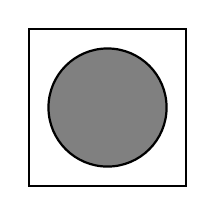
\begin{tikzpicture}
\draw[fill=white,thick](0,0) rectangle (2,2);
\draw[fill=gray,thick] (1,1) circle (0.75cm);
\end{tikzpicture}
\hspace{2cm}
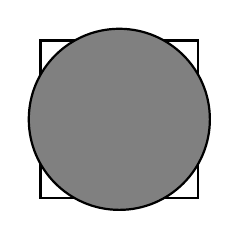
\begin{tikzpicture}
\draw[fill=white,thick](0,0) rectangle (2,2);
\draw[fill=gray,thick] (1,1) circle (1.15cm);
\end{tikzpicture}
\end{center}
\item Using the free electron model for a divalent crystal, the Fermi energy is
$$E_F=\frac{\hbar^2k_F^2}{2m}=\frac{\hbar^2}{2m}\bigg(\frac{2\sqrt{\pi}}{a}\bigg)^2=\frac{(6.626\times10^{-34}/2\pi)^2}{2(9.11\times10^{-31})}\frac{4\pi}{(0.4\times10^{-9})^2}=3.0eV$$
\item For [10] and [11] respectively, the zone boundaries are at $q=\pi/a$ and $q=\sqrt{2}\pi/a$, with $E_F=2.3$eV and $E_F=4.6$eV, as well as, a bandgap of 1eV for both.
\item The system will be an insulator if the highest energy in the lower band in the [11] direction is lower than the lowest energy in the higher band in the [10] direction. The least value of the highest energy in the lower band in [11] is $4.6-1.0=3.6$eV but the lowest energy in the higher band in [10] is $2.3+1.0=3.3$eV. The system will start to fill the states in the second band before completely filling in the first band, hence it is a metal.
\end{enumerate}
\end{ans}
\subsubsection{Section D}
\begin{qns}[OWO Short Notes]
Write brief notes on two of the following:\hfill\textbf{[20]}
\begin{itemize}
    \item wave impedance and impedance matching in the context of acoustic or mechanical waves;
    \item thin-film interference;
    \item Michelson's interferometer.
\end{itemize}
\end{qns}
\begin{ans}\leavevmode
\subsubsection*{Wave impedance and impedance matching in the context of acoustic or mechanical waves:}
Any medium through which waves propagate will present an impedance to those waves. If the medium is lossless, and possesses no resistive or dissipation mechanism, this impedance will be determined by the two energy storing parameters: inertia and elasticity, and it will be real. If there is a loss mechanism, the impedance will be complex.\\[5pt]
We proceed to discuss the heuristic derivation of wave impedance for a mechanical wave. Consider progressive waves on a string, generated say by an oscillating transverse force $F_0e^{i\omega t}$. The tension in the string is constant, $T$, and at the end of the string, the balance shows that the applied force is equal and opposite to $T\sin\theta$ $\forall t$, i.e. $F_0e^{i\omega t}=-T\sin\theta\approx -T\tan\theta=-T\frac{\partial y}{\partial x}$. The displacement of the progressive wave is $y=Ae^{i(\omega t-kx)}$ and so at the end of the string, say $x=0$, we have $F_0e^{i\omega t}=ikTAe^{i\omega t}$. We define the impedance to be the ratio of the force amplitude to velocity amplitude, which gives
$$Z=\frac{F_0}{v_0}=\frac{T}{c}=\rho c$$
where $v=\dot{y}=\frac{d}{dt}\frac{F_0}{i\omega}\frac{c}{T}e^{i(\omega t-kx)}\implies v_0=\frac{F_0c}{T}$, and from wave equation, $T=\rho c^2$.\\[5pt]
Next, we discuss the transmission of this wave through an interface separating two media of two different densities $\mu_1$ for $-\infty<x<0$ and $\mu_2$ for $0<x<\infty$, the transmission and reflection coefficients are $\frac{2v_2}{v_1+v_2}$ and $\frac{v_2-v_1}{v_2+v_1}$ respectively, where $v_i$ is the speed in medium $i$. This is obtained by imposing continuity of displacement across the interface and continuity of transverse force.\\[5pt]
The power transmitted across a given point on the string is $\mp Z(\frac{\partial\psi}{\partial t})^2=\mp vE(x,t)$, where $E$ is the energy per unit length and $Z$ is the impedance. Energy is still conserved for the previous situation, with the ratio of reflected energy to incident energy, and the ratio of transmitted energy to incident energy, are $(\frac{Z_1-Z_2}{Z_1+Z_2})^2$ and $\frac{4Z_1Z_2}{(Z_1+Z_2)^2}$ respectively.\\[5pt]
There are two basic ways to match two impedances. Either make one of them equal to the other, or keep them as they are but insert a large number of things between them with impedances that gradually change from one to the other. One example (beyond this mechanical wave example) is a particular lens coating that minimizes reflection of green light, giving it a characteristic purple color. By considering the former:\\[5pt]
In order to match the impedance between two media of impedances $Z_1$ ($x<0$) and $Z_3$ ($x>l$), we place a layer of medium of impedance $Z_2$, in the region $0\leq x\leq l$. For effective impedance matching, we require $Z_2=\sqrt{Z_1Z_3}$ and choose $l=\lambda_2/4$ (quarter-wavelength). When this is attained, the ratio of transmitted energy in $x>l$ to the incident energy in $x<0$ is equal to 1. 
\newpage
\subsubsection*{Thin film interference:}
Consider light incident (in medium 1) at an interface separating two media of refractive indices $n_1$ and $n_2$ where $n_2>n_1$, and the thickness of medium 2 is $t$. Since $n_2>n_1$, the ray reflected from this interface acquires a phase change of $\pi$ (otherwise, if $n_2<n_1$, no such phase change occurs). We assume the medium below medium 2 has a smaller refractive index. Let $n_1=1$ and $n_2=n$, the path difference is
$$n\bigg(\frac{t}{\cos\theta}+\frac{t}{\cos\theta}-(2t\tan\theta)\sin\theta_i\bigg)=\frac{2nt}{\cos\theta}-\frac{2nt\sin^2\theta}{\cos\theta}=2nt\cos\theta$$
where we used Snell's Law $\sin\theta_i=n\sin\theta$. The phase difference $\delta$ will be the path difference multiplied by $\frac{2\pi}{\lambda}$, plus the additional $\pi$ phase. If $\delta$ is a integer multiple of $2\pi$, i.e. $2nt\cos\theta\frac{2\pi}{\lambda}=(2m+1)\pi$, the beams are in phase and bright fringes are observed. Conversely, $2nt\cos\theta\frac{2\pi}{\lambda}=2m\pi$, the beams are in anti-phase and dark fringes are observed. \\[5pt]
If the two interfering beams differ in strength, the fringes are still present with the same period, but are less distinct (contrast) since they sit on top of a constant background. With a beamsplitter, lens and extended source, circular fringes of equal inclination $\theta_i$, known as Haidinger fringes, may be observed.\\[5pt]
For films of non-uniform thickness, the corresponding interference fringes are known as fringes of equal thickness $t$. For a wedge, the resulting interference fringes are localized near and are almost parallel to the thin end of the wedge. For soap films, when illuminated with white light, each wavelength component produces its own set of fringes with a different period. The superposition of these fringes leads to a complex pattern of colours across the film.
\begin{figure}[H]
\centering
\includegraphics[width=\linewidth]{thinfilm.PNG}
\end{figure}
\newpage
\subsubsection*{Michelson's interferometer:}
The Michelson interferometer has many important applications including high precision metrology, Fourier Transform spectroscopy and the Michelson-Morley experiment. Consider the basic setup
\begin{figure}[H]
    \centering
    \includegraphics[width=\linewidth]{mmi.PNG}
\end{figure}
The beam-splitter splits the incident beam with components travel along different paths, and recombine at the same beam-splitter. Constructive or destructive interference will occur depending on the difference between the two paths. Normally, one path is kept fixed (reference path) and the other path is varied by moving a mirror (on a precision stage) in order to see a fringe pattern as a function of the mirror position. This arrangement focuses the beams onto a photodiode. The system is illuminated with the collimated beam; the mirrors are aligned so that the path difference is constant across the beam\\[5pt]
For an extended light source, light from different parts of the source travels at different angles through the interferometer to the eye and the differential delays will be a function of this angle. Mirrors may also be tilted to introduce different delays for beams hitting the mirrors at different points. The combination of these effects means that a spatially-varying intensity (i.e. fringes) can be seen when the mirrors are both held fixed.\\[5pt]
If monochromatic light was used: $x=\frac{\delta}{k}$ is twice the difference in distances of the two mirrors from the beamsplitter. If the interfering beams have equal intensities $0.5 I_0$, then we have $\langle I(x)\rangle=\langle I_0\rangle+\langle I_0\text{Re}(e^{ikx})\rangle$. If we vary $x$ linearly as a function of time, then the intensity seen at the output of the interferometer will vary sinusoidally, i.e. get a fringe pattern in time. This allow us to measure the wavelength of the monochromatic light used.\\[5pt]
If the light is not monochromatic, each wavelength will form its own set of fringes and there will be no fringes corresponding to interference between different wavelengths. As we vary $x$, we see fringe contrast change. In fact, we get a blurred, coloured pattern. Let the intensity of light in the wavenumber range $[k,k+dk]$ be $2S(k)dk$, then the total intensity observed (implicit time-averaged) will be the sum of all the sine waves weighted by the intensity at the relevant wavelength:
$$I(x)=2\int_0^\infty S(k)(1+\text{Re}[e^{ikx}])dk$$
We can also define $S(k)$ for negative $k$, such that $S(-k)=S^*(k)$, hence drop the factor of 2 and let the integration range be from $k=-\infty$ to $k=\infty$. We have
$$I(x)=\int_{-\infty}^\infty S(k)(1+e^{ikx})dk=I_1+\int_{-\infty}^\infty S(k)e^{ikx}dk$$
where $I_1=\int_{-\infty}^\infty S(k)dk$ is equal to the total intensity of the light. $S(k)$ can thus be found using inverse Fourier transform:
$$S(k)=\frac{1}{2\pi}\int_{-\infty}^\infty(I(x)-I_1)e^{-ikx}dk$$
A useful applicable feature of the interferometer is its high resolution. If a light source has two closely-spaced wavelengths $k_0\pm\Delta k$, each component will produce a fringe pattern with a slightly different fringe spacing. The observed interference pattern will be the sum of the two individual patterns. As $x$ increases from $x=0$, a phase shift develops between the two patterns and eventually the fringes become invisible since the maxima in one set of fringes overlap with the minima in the other set. The larger the spacing between the components $\Delta k$, the more rapidly fringes disappear as $x$ increases.\\[5pt]
In our double-sided convention for a spectrum, $S(k)$ can be represented as two pairs of closely-spaced delta functions spaced about $\pm k_0$. This can be written as a convolution $S(k)=[\delta(k-k_0)+\delta(k+k_0)]*[\delta(k-\Delta k)+\delta(k+\Delta k)]\implies I(x)=I_1[1+\cos(k_0x)\cos(\Delta kx)]$. The high frequency cosine $\cos(k_0x)$ represents the fringes while the low frequency envelope $\cos(\Delta kx)$ modulates the amplitude of these fringes. We can define the fringe contrast or fringe visibility as the ratio of local high-frequency fringe amplitude to the mean intensity.
$$\frac{I_{max}-I_{min}}{I_{max}+I_{min}}$$
At the position of the first zero in the low frequency envelope, the fringe contrast will be zero and this can be used to find $\Delta k$.\\[5pt]
Measuring the fringe visibility allows the fine structure of atomic lines to be investigated. The Sodium D line at 589.3 nm is in fact a doublet with $\Delta\lambda=0.6$ nm, whereas the Cadmium line is highly monochromatic, hence showing no minimum in fringe visibility for values of $x\leq 0.4$ m.
\end{ans}
\newpage
\begin{qns}[CMP Essay]
Write an essay on the physics of the semiconductor n-p junction and its uses. Your discussion should include the effect of doping, the formation of a depletion layer, and the origin of the ideal diode I-V characteristic.\hfill\textbf{[20]}
\end{qns}
\begin{ans}
Adding dopants that gives more (fewer) electrons than the substrate itself creates an n-type (a p-type) semiconductor. At non-zero temperatures, all these states are ionized, increasing the conductance of the material. For the n-type (p-type), the vast majority of the charge carriers are ionized electrons (holes left behind when electrons from the filled band were excited into the dopant hole state). In the absence of impurities, the Fermi energy ($\mu(T=0)$) is in the middle of the band gap. When the donor (acceptor) impurities are added, at zero temperature, impurity states near the top (bottom) of the bandgap are filled (empty). The Fermi energy is moved up to the top (down to the bottom) of the band gap.\\[5pt]
Although the n-doped system has free negatively charged electrons and the p-doped system has free positively charged holes, both systems are overall electrically neutral since charged ions compensate for the charges of the mobile charge carriers. When the two doped semiconductors are brought into contact, the electrons in the conduction band will fall into the valence band, filling the empty hole states, thus pair-annihilating both the electron and the hole. This amounts to a gain in energy of $E_{gap}$ per pair annihilated.\\[5pt]
After this process of electrons falling into holes and annihilating occurs there will be a region near the interface where there are no free carriers at all. This is the depletion region, which is electrically charged (since there are charged ions but no carriers to neutralize them). Hence, there is a net electric field pointing from the positively charged to the negatively charged ions.\\[5pt]
We now imagine moving an additional electron across the depletion region in order to annihilate another hole. While the annihilation process gives a gain in energy of $E_{gap}$, the process of moving the electron across the depletion region costs an energy of $-e\Delta\phi$, where $\phi$ is the electrostatic potential. When the depletion region is sufficiently large, it becomes no longer favorable for further electrons and holes to annihilate. \\[5pt]
Rectification: allow current to flow through the junction easily in one direction, but not the other. There are 4 processes that can create current:
\begin{enumerate}
    \item Electrons may be thermally excited into the conduction band. Some of these electrons will flow down the slope to the left.
    \item Holes may be thermally excited down into the valence band and will flow up the slope to the right. 
    \item Electrons in the conduction band on the left will be thermally activated to climb up the potential slope in the depletion layer and will annihilate with holes once they arrive at the p-doped side. 
    \item Holes in the valence band on the right may be thermally activated to climb down the potential slope towards the n-doped side where they annihilate with electrons.
\end{enumerate}
The contribution by processes 1 and 2 to the current is directly proportional to $e^{-E_{gap}/k_BT}$. Voltage bias will not change the number of excited carriers, hence current independent of voltage. The contribution by processes 3 and 4 to the current is directly proportional to $e^{-E_{gap}/k_BT}$ in the absence of an applied voltage, and $e^{-(E_{gap}+eV)/k_BT}$ in the presence of an applied voltage. The total current flow will be the sum and hence
$$I=J_s(T)(e^{-eV/k_BT}-1)$$
where $J_s$ is directly proportional to $e^{-E_{gap}/k_BT}$ is known as the saturation current. This is the diode equation. Current flows easily in one direction, i.e. forward biased, but flows poorly in the opposite direction, i.e. reverse biased.
\begin{figure}[H]
    \centering
    \includegraphics[width=\linewidth]{pnjunction.PNG}
    \caption{Description of PN Junction. The drop in band energy is precisely compensated by the change in electrostatic potential. Image credit: CMP Notes by Cavendish.}
\end{figure}
\begin{figure}[H]
    \centering
    \includegraphics[width=\linewidth]{biasedPN.PNG}
    \caption{Band diagram of a biased p-n junction. The four processes that can create current are labelled. In the absence of applied voltage, the net current is zero. When voltage is applied, current flows easily for $eV<0$ and not easily with $eV>0$. Image from S.H. Simon: The Oxford Solid State Basics. }
\end{figure}
\end{ans}
\newpage
\section{2015}
\subsection{Paper 1}
\subsubsection{Section A}
\begin{qns}[1D Potential]
A particle is described by a wavefunction $\psi(x)=a+ix$ in the region $0<x<a$ and $\psi=0$ elsewhere. Calculate the probability of finding the particle in the region $a/2<x<a$.\hfill\textbf{[4]}
\end{qns}
\begin{ans}
The probability is
$$P(0.5a\leq x\leq a)=\frac{\int_{a/2}^a|\psi|^2dx}{\int_0^a|\psi|^2dx}=\frac{\int_{a/2}^aa^2+x^2dx}{\int_0^aa^2+x^2dx}=\frac{19}{32}$$
\end{ans}
\begin{qns}[Harmonic Oscillator]
Sketch the wavefunctions and corresponding energies of the eigenstates of a quantum harmonic oscillator, labelling your diagram to explain the key physical features.\hfill\textbf{[4]}
\end{qns}
\begin{ans}
The energy of the $n$th excited state of a quantum harmonic oscillator is $\hbar\omega(n+0.5)$. In sketching the harmonic oscillator wavefunctions, do note:
\begin{itemize}
    \item they are eigenstates of the parity operator, i.e. for the $n$th excited state, if $n$ is odd (even), the wavefunction $\psi$ exhibit odd (even) symmetry;
    \item the $n$th excited state has $n$ number of nodes, with the ground state having no nodes;
    \item the higher the kinetic energy (region of smaller potential), the shorter the wavelength;
    \item the point of inflexion occur when the kinetic energy is zero (transition between classically allowed and classically forbidden region).
\end{itemize}
\begin{figure}[H]
    \centering
    \includegraphics[width=\linewidth]{2015P1A2.JPG}
    \caption{The norm of the wavefunctions of harmonic oscillator, superimposed with the harmonic oscillator potential.}
\end{figure}
For very high $n$, one can also illustrate the correspondence principle (small amplitude when speed is large and high amplitudes when potential is large).
\end{ans}
\begin{qns}[Angular Momentum]
Show that, in spherical polar coordinates, the operator for the $z$-component of the orbital angular momentum is given, in spherical coordinates, by $-i\hbar\frac{\partial}{\partial\phi}$.

\hfill\textbf{[4]}
\end{qns}
\begin{ans}
Take the $z$-component of the angular momentum:
$$\mathbf{\hat{z}}\cdot\mathbf{\hat{L}}=\mathbf{\hat{z}}\cdot(\mathbf{\hat{r}}\times(\mathbf{\hat{p}_r}+\mathbf{\hat{p}_\theta}+\mathbf{\hat{p}_\phi}))=\mathbf{\hat{z}}\cdot(\mathbf{\hat{r}}\times\mathbf{\hat{p}_\phi})=(\mathbf{\hat{z}}\times\mathbf{\hat{r}})\cdot\mathbf{\hat{p}_\phi}=r\sin\theta\frac{\hbar}{i}\frac{1}{r\sin\theta}\frac{\partial}{\partial\phi}=-i\hbar\frac{\partial}{\partial\phi}$$
\end{ans}
\newpage
\begin{qns}[Error Analysis]
Stellar magnitudes, $m$, are determined by the equation $m=-2.5\log_{10}(f/f_0)$ with $f$ the stellar flux, and $f_0$ a normalization constant. Given a fractional error of 10\% in the stellar flux measurement, find the corresponding fractional error in $m$.\hfill\textbf{[4]}
\end{qns}
\begin{ans}
The error in $m$ is
$$\sigma_m^2=\bigg(\frac{\partial m}{\partial f}\bigg)^2\sigma_f^2\implies\sigma_m=\bigg|-\frac{2.5}{\ln(10)}\bigg|\bigg|\frac{\sigma_f}{f}\bigg|=\frac{2.5\times0.1}{\ln(10)}=0.109$$
The fractional error is $\sigma_m/m$, but we are not given $f$...
\end{ans}
\begin{qns}[Op-Amp and Filters]
For the following system containing an ideal op-amp, draw an annotated sketch of the gain $|V_{out}/V_{in}|$ as a function of frequency from 0.01 Hz to 100 Hz for a sinusoidal input.\hfill\textbf{[4]}
\end{qns}
\begin{figure}[H]
    \centering
    \includegraphics[scale=0.75]{2015P1A5Q.PNG}
\end{figure}
\begin{ans}
By the Golden Rules, we have $V_+=V_-$ and this gives
$$\frac{V_{in}-0}{r}=\frac{0-V_{out}}{Z}$$
where $\frac{1}{Z}=i\omega C+\frac{1}{R}$ and hence $\frac{V_{out}}{V_{in}}=-\frac{Z}{r}$. The gain would be
$$\frac{1}{G}=-\frac{r}{Z}=-\frac{r}{R}-i\omega rC\implies\bigg|\frac{1}{G}\bigg|=\sqrt{\frac{r^2}{R^2}+4\pi^2f^2r^2C^2}$$
so $|G|=\frac{10^3}{\sqrt{1+4\pi^2f^2}}$, where $\frac{r}{R}=\frac{1}{1000}$ and $RC=1$. Hence, $G(f=0)=10^3$ and there is a point of inflection at $G(f=\frac{2\pi}{\sqrt{3}})=44$.
\end{ans}
\newpage
\subsubsection{Section B}
\begin{qns}[1D Potential]\leavevmode
\begin{enumerate}[label=(\roman*)]
\item The particle flux associated with wavefunction $\psi$ is given by
$$J=\text{Re}\bigg[\psi^*\frac{\hbar}{im}\boldsymbol{\nabla}\psi\bigg]$$
where $m$ is the mass of the particle. Find the particle flux associated with a plane wave $Ae^{i(kx-\omega t)}$.\hfill\textbf{[3]}
\item A region of space contains two superimposed plane waves propagating in opposite directions:
$$\psi=Ae^{i(kx-\omega t)}+Be^{i(-kx-\omega t)}$$
where $A$ and $B$ are complex constants. By explicitly evaluating the expression for particle flux above, show that the net particle flux in this region is equal to the difference in fluxes of the forward- and backward-propagating waves in isolation.\hfill\textbf{[6]}
\item A particle of kinetic energy $E$ and mass $m$ is incident on a potential step of height $V$, as shown below. Calculate the amplitude reflection coefficient, $r_a$, and the amplitude transmission coefficient, $t_a$, as a function of $E$ and $V$.\hfill\textbf{[5]}
\begin{figure}[H]
    \centering
    \includegraphics[scale=0.75]{2015P1B6Q.PNG}
\end{figure}
\item Show that the net particle flux in Region 1 is equal to the transmitted particle flux in Region 2.\hfill\textbf{[3]}
\item Evaluate the transmission probability for electrons, when $E = 3$ eV and $V = 2$ eV.\hfill\textbf{[3]}
\end{enumerate}
\end{qns}
\begin{ans}\leavevmode
\begin{enumerate}[label=(\roman*)]
\item $\boldsymbol{\nabla}\psi=\frac{\partial}{\partial x}\psi\mathbf{\hat{x}}=ik Ae^{i(kx-\omega t)}\mathbf{\hat{x}}$. Then,
$$\mathbf{J}=\text{Re}\bigg[Ae^{-i(kx-\omega t)}\frac{\hbar}{im}ikAe^{i(kx-\omega t)}\bigg]\mathbf{\hat{x}}=\frac{\hbar k}{m}|A|^2\mathbf{\hat{x}}$$
\item $\frac{\partial}{\partial x}\psi=ik(Ae^{i(kx-\omega t)}-Be^{-i(kx+\omega t)})$, then $\mathbf{J}=\frac{\hbar k}{m}(|A|^2-|B|^2)\mathbf{\hat{x}}$, which is equal to the sum of the forward propagating flux $\frac{\hbar k}{m}|A|^2$ and the backward propagating flux $-\frac{\hbar k}{m}|B|^2$.
\item Let the step be at $x=0$. We guess $\psi$ to have an asymptotic form
$$\psi(x)=
\left\{
        \begin{array}{ll}
      e^{i(k_1x-\omega t)}+r_ae^{-i(k_1x+\omega t)} & x<0\\
      t_a e^{i(k_2x-\omega t)} & x>0
        \end{array}
    \right.$$ 
where $k_1=\frac{\sqrt{2mE}}{\hbar}$ and $k_2=\frac{\sqrt{2m(E-V)}}{\hbar}$. The boundary conditions at $x=0$ are
\begin{itemize}
    \item $\psi$ is continuous: $1+r_a=t_a$;
    \item $\psi'$ is continuous: $ik_1(1-r_a)=ik_2t_a$.
\end{itemize}
Solving them gives $$r_a=\frac{1-(k_2/k_1)}{1+(k_2/k_1)}=\frac{1-\sqrt{1-\frac{V}{E}}}{1+\sqrt{1-\frac{V}{E}}}$$
$$t_a=\frac{2}{1+(k_2/k_1)}=\frac{2}{1+\sqrt{1-\frac{V}{E}}}$$
where $\frac{k_2}{k_1}=\sqrt{1-\frac{V}{E}}$.
\item From part(ii), the net particle flux in region 1 is 
$$\frac{\hbar k_1}{m}(1-|r_a|^2)=\frac{\hbar k_1}{m}\bigg(1-\bigg(\frac{1-\frac{k_2}{k_1}}{1+\frac{k_2}{k_1}}\bigg)^2\bigg)=\frac{\hbar k_1}{m}\frac{1}{(1+\frac{k_2}{k_1})^2}\frac{4k_2}{k_1}=\frac{4\hbar k_2}{m(1+\frac{k_2}{k_1})^2}$$
From part(i), the net particle flux in region 2 is
$$\frac{\hbar k_2}{m}|t_a|^2=\frac{\hbar k_2}{m}\frac{4}{(1+\frac{k_2}{k_1})^2}$$
This is equal to the previous result.
\item The transmission probability $T$ is the ratio of transmitted flux $\frac{\hbar k_2}{m}|t_a|^2$ to the incident flux $\frac{\hbar k_1}{m}$.
$$T=|t_a|^2=\frac{4\frac{k_2}{k_1}}{(1+\frac{k_2}{k_1})^2}=\frac{2\sqrt{3}}{2+\sqrt{3}}=0.93$$
where $E=3$ eV, $V=2$ eV, and so $\frac{k_2}{k_1}=\frac{1}{\sqrt{3}}$.
\end{enumerate}
\end{ans}
\newpage
\begin{qns}[1D Potential]\leavevmode
\begin{enumerate}[label=(\roman*)]
\item An infinitely deep quantum well extends from $x = 0$ to $x = a$, and contains a particle of mass $m$. Find the energies and normalised wavefunctions of the eigenstates of the system, as a function of the quantum number $n=1,2,3,...$.\hfill\textbf{[6]}
\item A particle is in the ground state of a quantum well of width $a$. The quantum well suddenly expands to a width $2a$, leaving the wavefunction unchanged. The energy of the system is then immediately measured. Calculate the probability that the system will be found in the ground state of the expanded well.\hfill\textbf{[6]}
\item At time $t = 0$, the system is in an eigenstate of the Hamiltonian, $|\phi_n\rangle$, with energy $E_n$. Using the time-dependent Schrodinger equation, find the wave function at time $t$.\hfill\textbf{[4]}
\item For the quantum well system above, describe in general terms how you would calculate the probability of finding the system in the new ground state if a time $t$ elapses between the expansion and the measurement.\hfill\textbf{[4]}
\end{enumerate}
\end{qns}
\begin{ans}\leavevmode
\begin{enumerate}[label=(\roman*)]
\item Integrating the Schrodinger equation over an infinitesimal range $[\mu,\mu+\epsilon]$ for arbitrary $\mu$ and small $\epsilon$, 
$$-\frac{\hbar^2}{2m}\bigg[\frac{\partial\psi}{\partial x}\bigg]_\mu^{\mu+\epsilon}+V(\mu)\psi(\mu)\epsilon=E\psi(\mu)\epsilon$$
Suppose the potential is a reasonable infinity such that $V(\mu)\epsilon$ is either finite or zero as $\epsilon\rightarrow 0$, then the gradient is continuous everywhere. But $\psi$ is required to be continuous everyhwere. For $\psi\neq 0$ in $0\leq x\leq a$, $\psi\neq 0$ in a region where $V\neq 0$, resulting in infinite potential energy, a contradiction. Hence, $\psi$ must be zero in the region of infinite potential region, thus giving the boundary conditions $\psi(x=0,t)=0$ and $\psi(x=a,t)=0$. In this case, the Schrodinger equation $\frac{d^2\psi}{dx^2}=-\frac{2mE}{\hbar^2}\psi<0$ gives us $\psi=A\sin\frac{n\pi x}{a}$, where $A$ is the normalization constant.
$$1=\int_0^a|A|^2\bigg[\frac{1}{2}-\frac{1}{2}\cos\bigg(\frac{2n\pi x}{a}\bigg)\bigg]dx\implies |A|=\sqrt{\frac{2}{a}}$$
\item The new ground state is $\sqrt{\frac{2}{2a}}\sin\frac{\pi x}{2a}$ while the old ground state is $\sqrt{\frac{2}{a}}\sin\frac{\pi x}{a}$. The probability of transition is
$$\bigg|\int_0^a\frac{2}{a\sqrt{2}}\sin\frac{\pi x}{a}\sin\frac{\pi x}{2a}dx\bigg|^2=\frac{2}{a^2}\bigg|\int_0^a\frac{1}{2}\bigg(\cos\frac{\pi x}{2a}-\cos\frac{3\pi x}{2a}\bigg)dx\bigg|^2=\frac{2}{\pi^2}\bigg(1+\frac{1}{3}\bigg)^2=0.36$$
\item The time-dependent Schrodinger equation is $i\hbar\frac{\partial\psi}{\partial t}=E_n\psi\implies\psi\propto e^{-iE_nt/\hbar}$, and so
$$\psi(x,t)=\sqrt{\frac{2}{a}}e^{-i\frac{n^2\hbar\pi^2t}{2ma^2}}\sin\frac{n\pi x}{a}$$
\item The old ground state is now a linear combination of the energy eigenfunctions of the new system at $t=0$, i.e.
$$|\psi_{old,ground}(t=0)\rangle=\sum_{n=1}^\infty\langle\psi_{new,n}|\psi_{ground}(t=0)\rangle|\psi_{new,n}\rangle\implies$$
$$|\psi_{old,ground}(t)\rangle=\sum_{n=1}^\infty e^{-iE_nt\hbar}\langle\psi_{new,n}|\psi_{ground}(t=0)\rangle|\psi_{new,n}\rangle$$
where the different phase factor is added to each individual basis function. The probability remains unchanged for $t>0$ since $|e^{-iE_nt/\hbar}|=1$.
\end{enumerate}
\end{ans}
\newpage
\begin{qns}[Harmonic Oscillator]\leavevmode
\begin{enumerate}[label=(\roman*)]
\item Show that the Hamiltonian for a particle of mass $m$ in a one-dimensional potential $\frac{1}{2}m\omega^2x^2$ can be written in the form 
$$\hat{H}=\bigg(\hat{a}^\dag\hat{a}+\frac{1}{2}\bigg)\hbar\omega$$
where $\hat{a}=\sqrt{\frac{m\omega}{2\hbar}}(\hat{x}+i\frac{\hat{p}}{m\omega})$ and $\hat{a}^\dag=\sqrt{\frac{m\omega}{2\hbar}}(\hat{x}-i\frac{\hat{p}}{m\omega})$.\hfill\textbf{[5]}
\item Evaluate the commutators $[\hat{a},\hat{a}^\dag]$, $[\hat{H},\hat{a}]$ and $[\hat{H},\hat{a}^\dag]$.\hfill\textbf{[5]}
\item The state $|\phi\rangle$ is an eigenstate of $\hat{H}$ with energy $E$. Show that $\hat{a}^\dag|\phi\rangle$ is also an
eigenstate of $\hat{H}$, and find its energy.\hfill\textbf{[4]}
\item Given that $\hat{a}|0\rangle=0$, find (unnormalised) wavefunctions for the ground state, $|0\rangle$, and for the first excited state, and verify that these are orthogonal.\hfill\textbf{[6]}
\end{enumerate}
\end{qns}
\begin{ans}\leavevmode
\begin{enumerate}[label=(\roman*)]
\item Evaluate $\hat{a}\hat{a}$:
$$\hat{a}^\dag\hat{a}=\bigg(\sqrt{\frac{m\omega}{2\hbar}}\hat{x}-i\frac{1}{\sqrt{2m\hbar\omega}}\hat{p}\bigg)\bigg(\sqrt{\frac{m\omega}{2\hbar}}\hat{x}+i\frac{1}{\sqrt{2m\hbar\omega}}\hat{p}\bigg)=\bigg(\frac{m\omega}{2\hbar}\hat{x}^2+\frac{1}{2m\hbar\omega}\hat{p}^2\bigg)+i[\hat{x},\hat{p}]\sqrt{\frac{m\omega}{2m2\hbar\hbar\omega}}$$
Then, $\hbar\omega(\hat{a}^\dag\hat{a}+0.5)=\frac{1}{2}m\omega^2\hat{x}^2+\frac{\hat{p}^2}{2m}$, which is consistent with the Hamiltonian of harmonic oscillator.
\item The commutators are
$$[\hat{a},\hat{a}^\dag]=\sqrt{\frac{m\omega}{2\hbar}}\frac{-i}{\sqrt{2m\hbar\omega}}[\hat{x},\hat{p}]+i\sqrt{\frac{m\omega}{2\hbar}}\frac{1}{\sqrt{2m\hbar\omega}}[\hat{p},\hat{x}]=\frac{2}{2\hbar}i\hbar(-i)=1$$
$$[\hat{H},\hat{a}]=\hbar\omega[\hat{a}^\dag\hat{a},\hat{a}]=\hbar\omega[\hat{a}^\dag,\hat{a}]\hat{a}=-\hbar\omega\hat{a}$$
$$[\hat{H},\hat{a}^\dag]=\hbar\omega[\hat{a}^\dag\hat{a},\hat{a}^\dag]=\hbar\omega\hat{a}^\dag[\hat{a}^\dag,\hat{a}]=+\hbar\omega\hat{a}^\dag$$
\item Using the result of part (i):
$$\hat{H}\hat{a}^\dag|\phi\rangle=(\hat{a}^\dag\hat{H}+[\hat{H},\hat{a}^\dag])|\phi\rangle=(\hat{a}^\dag\hat{H}+\hbar\omega\hat{a}^\dag)|\phi\rangle=(E+\hbar\omega)\hat{a}^\dag |\phi\rangle$$
Indeed, $\hat{a}^\dag|\phi\rangle$ is an eigenstate of $\hat{H}$ with energy $E+\hbar\omega$.
\item Solving the operator differential equation:
$$0=\hat{a}|0\rangle=\bigg(\sqrt{\frac{m\omega}{2\hbar}}\hat{x}+\sqrt{\frac{\hbar}{2m\omega}}\frac{\partial}{\partial x}\bigg)|0\rangle\implies\frac{d}{dx}|0\rangle=-\frac{m\omega}{\hbar}|0\rangle$$
which gives us the ground state $$|0\rangle=A_0 e^{-m\omega x^2/2\hbar}$$ for some normalization constant $A_0$. We obtain the first excited state by acting $\hat{a}^\dag$ on the ground state $|0\rangle$.
$$\sqrt{1}|1\rangle=\hat{a}^\dag|0\rangle=A_0\bigg(\sqrt{\frac{m\omega}{2\hbar}}\hat{x}-i\frac{1}{\sqrt{2m\hbar\omega}}\hat{p}\bigg)e^{-m\omega x^2/2\hbar}=A_0e^{-\frac{m\omega x^2}{2\hbar}}\bigg(\sqrt{\frac{m\omega}{2\hbar}}x-\frac{\hbar}{\sqrt{2m\hbar\omega}}\frac{-m\omega x}{\hbar}\bigg)$$
The first excited state will thus be
$$|1\rangle=A_0\sqrt{\frac{2m\omega}{\hbar}}xe^{-m\omega x^2/2\hbar}$$
To check orthogonality:
$$\langle 1|0\rangle=|A_0|^2\int_{-\infty}^\infty e^{-m\omega x^2/\hbar}\sqrt{\frac{2m\omega}{\hbar}}xdx=0$$
since the integrand is odd and we are integrating over symmetric limits.
\end{enumerate}
\end{ans}
\newpage
\begin{qns}[Identical Particles]\leavevmode
\begin{enumerate}[label=(\roman*)]
\item For a system of two identical particles, explain what constraint is placed on the overall wavefunction by considering the operation of exchanging the two particles.\hfill\textbf{[3]}
\item For a system of two fermions whose wavefunction can be written as the product of a spatial part and a spin part, explain what are the possible combinations of exchange symmetries for the spatial and spin parts of the wavefunction.\hfill\textbf{[3]}
\item Consider the hydrogen molecule H$_2$. Explain what is meant by para-hydrogen and ortho-hydrogen.\hfill\textbf{[2]}
\item The total angular momentum of a hydrogen molecule is described by the quantum number $\ell$. Show that $\ell$ can only take even values for para-hydrogen and odd values for ortho-hydrogen.

\hfill\textbf{[4]}
\begin{mdframed}
\color{darkblue}{The spherical harmonic functions $Y_{l,m}(\theta,\phi)$ have the property $Y_{l,m}(\pi-\theta,\phi+\pi)=(-1)^lY_{l,m}(\theta,\phi)$.}
\end{mdframed}
\item When liquid hydrogen is prepared, it consists of 25\% para-hydrogen with $\ell=0$ and 75 percent ortho-hydrogen with $\ell = 1$. Over a period of days, the ortho-hydrogen converts to the lower-energy para-hydrogen state. Calculate the energy released when this occurs in 1 kg of liquid hydrogen. \hfill\textbf{[6]}

\begin{mdframed}
\color{darkblue}{The bond length in the hydrogen molecule is 74 pm.}
\end{mdframed}
\item Comment on the consequences for storage of liquid hydrogen.\hfill\textbf{[2]}
\end{enumerate}
\end{qns}
\begin{ans}\leavevmode
\begin{enumerate}[label=(\roman*)]
\item Since the particles are identical, all observed quantities must be invariant under particle exchange, and so the overall wavefunctions must be eigenstates of the particle exchange operator $\hat{P}_{ij}$ with an eigenvalue of unit modulus. But $\hat{P}_{ij}^2=1$, so the eigenvalues must square to unity (cannot be complex conjugates), and so it has to be $\pm1$. When the eigenvalue is $+1$ ($-1$), the identical particles have even (odd) symmetry under exchange. These particles are called bosons (fermions) and by Spin-Statistics Theorem, they have integer (half-integer) spins.
\item From part (i), the fermions' overall wavefunction must be anti-symmetric under particle exchange. Thus, it can only be the product of symmetric spatial part and anti-symmetric spin part.
\item Para and ortho Hydrogen have $s_{total}=$ 0 and 1 respectively.
\item The two protons in H$_2$ are each spin $\frac{1}{2}$ and thus identical to the scenario in part (ii). For $s_{total}=1$, there are 3 possible states since $-s_{total}\leq m_s\leq s_{total}$:
\begin{itemize}
    \item $|s=1,m_s=1\rangle$: $|\uparrow\rangle|\uparrow\rangle$;
    \item $|s=1,m_s=0\rangle$: $|\uparrow\rangle|\downarrow\rangle$ or $|\downarrow\rangle|\uparrow\rangle$;
    \item $|s=1,m_s=-1\rangle$: $|\downarrow\rangle|\downarrow\rangle$;
\end{itemize}
For $s_{total}=0$, $m_s=0$, and we can have either $|\uparrow\rangle|\downarrow\rangle$ or $|\downarrow\rangle|\uparrow\rangle$. But $s_{total}=1$ is symmetric under particle exchange, so we choose a linear combination such that it is symmetric under exchange:
$$|s=1,m_s=0\rangle=\frac{1}{\sqrt{2}}(|\uparrow\rangle|\downarrow\rangle+|\downarrow\rangle|\uparrow\rangle)$$
Similarly, $s_{total}=0$ is anti-symmetric under particle exchange:
$$|s=0,m_s=0\rangle=\frac{1}{\sqrt{2}}(|\uparrow\rangle|\downarrow\rangle-|\downarrow\rangle|\uparrow\rangle)$$
Now use centre-of-mass coordinates such that their mutual Coulomb force of repulsion is a central force. The spherical harmonics, functions of $\theta$ and $\phi$, are thus appropriate to describe the angular dependence of the wavefunction in this system. The exchange of physical positions of the two protons is equivalent to spatial inversion with respect to the origin:
$$R(r)Y_{l,m}(\theta,\phi)\mapsto R(r)Y_{lm}(\pi-\theta,\pi+\phi)=R(r)(-1)^lY_{l,m}(\theta,\phi)\implies\psi(r,\theta,\phi)\mapsto\psi(r,\theta,\phi)(-1)^l$$
which suggests $l$ must be even (odd) for even (odd) symmetry.
\item The energy of a classical rigid rotor is $E_L=\frac{L^2}{2I}$ and so the Hamiltonian of a quantum rigid rotor is $\hat{H}=\frac{\hat{L}^2}{2I}$ with eigenvalues $E_l=\frac{\hbar^2l(l+1)}{2I}$ and so the energy intervals are $\Delta E=E_{l+1}-E_l=\frac{\hbar^2}{2I}[(l+1)(l+2)-l(l+1)]=\frac{\hbar^2}{I}(l+1)$. For $l=0$, $\Delta E=\frac{\hbar^2}{I}$. The transition is from $l=1$ ortho to $l=0$ para. Furthermore, the moment of inertia $I$ for H$_2$ is $I=m(a/2)^2+m(a/2)^2=\frac{1}{2}ma^2$. The total energy released is $$75\%\times\frac{1}{2(1.67\times10^{-27})}\frac{(6.626\times10^{-34}/2\pi)^2}{0.5(1.6\times10^{-27})(24\times10^{-12})^2}=5.5\times10^5J$$
\item Depends on how quickly (kinetics) this process occurs and how easily one can conduct away the excess heat.
\end{enumerate}
\end{ans}
\newpage
\subsubsection{Section C}
\begin{qns}[QM Essay]
Write an essay on the use of the density operator in quantum mechanics.\hfill\textbf{[20]}
\end{qns}
\begin{ans}
A first course in quantum mechanics will portray a simplistic picture of quantum systems, where we somehow always know which state our system is in - it may be a simple eigenstate of some operator or else a superposition. There may actually be some classical uncertainty in our knowledge: Suppose we only know our system is in some state $|\Psi_i\rangle$ with probability $p_i$. Here, $|\Psi_i\rangle$
\begin{itemize}
\item do not have to be eigenstates of any Hamiltonian operator.
\item do not have to obey $\langle\Psi_i|\Psi_j\rangle=0$, so long as they are distinct.
\item do not need to be a complete set, i.e. the following is not always true: $|\Psi\rangle=\sum_i\sqrt{p_i}|\Psi_i\rangle$. 
\end{itemize}
If we compute the expectation value of some $A$, we have
$$\langle A\rangle=\sum_ip_i\langle\Psi_i|A|\Psi_i\rangle$$
This includes quantum uncertainty, since $|\Psi_i\rangle$ might not be an eigenstate of $A$. A neater way would be to introduce the density operator. We define the density operator $\rho:~\mathcal{H}\rightarrow\mathcal{H}$ to be
$$\rho=\sum_ip_i|\Psi_i\rangle\langle\Psi_i|$$
where $\mathcal{H}$ is the Hilbert space. The density operator obeys $\rho^\dag=\rho$ since probabilities are real. Take the trace over the entire Hilbert space will give $\Tr_{\mathcal{H}}\rho=1$ since probabilities sum to 1. Finally, $\langle\chi|p|\chi\rangle\geq0$ $\forall|\chi\rangle\in\mathcal{H}$ since probabilities are non-negative. Essentially, the density operator is a positive semi-definite operator, i.e. $\rho\geq0$. Using the definition of trace, we can write the expectation in terms of the density operator.
$$\langle Q\rangle:=\Tr_{\mathcal{H}}(Q\rho)=\sum_n\langle q_n|\rho Q|q_n\rangle=\sum_np_\alpha\langle q_n|\psi_\alpha\rangle\langle\psi_\alpha|Q|q_n\rangle$$
where we used $|\psi_\alpha\rangle\langle\psi_\alpha|=\text{Id}_{\mathcal{H}}$. The result follows from the cyclic property of trace. We apply our understanding to a simple example of a two-level system. Suppose we have a two-state system (qubit) with basis states $\{|\uparrow\rangle,|\downarrow\rangle\}$. If $\rho=|\uparrow\rangle\langle\uparrow|$, the system is definitely in the state $|\uparrow\rangle$, hence a pure state. If $\rho=\frac{1}{2}|\uparrow\rangle\langle\uparrow|+\frac{1}{2}|\downarrow\rangle\langle\downarrow|=\frac{1}{2}\text{Id}$, the state is equally likely to be in $|\uparrow\rangle$ or $|\downarrow\rangle$. We are not saying $|\Psi\rangle=\frac{1}{\sqrt{2}}(|\uparrow\rangle+|\downarrow\rangle)$! This is an impure or a mixed state. We could also have $\rho=\frac{1}{2}|\uparrow\rangle\langle\uparrow|+\frac{1}{2}|\uparrow_x\rangle\langle\uparrow_x|$, where $S_x|\uparrow_x\rangle=\frac{\hbar}{2}|\uparrow_x\rangle$. Note that $\langle\uparrow_x|\uparrow\rangle\neq0$. In this case, since $|\uparrow_x\rangle=\frac{1}{\sqrt{2}}(|\uparrow\rangle+|\downarrow\rangle)$, we can write this as
$$\rho=\frac{1}{4}\text{Id}_{\mathcal{H}}+\frac{1}{2}|\uparrow\rangle\langle\uparrow|+\frac{1}{4}|\uparrow\rangle\langle\downarrow|+\frac{1}{4}|\downarrow\rangle\langle\uparrow|$$
showing that
$$\rho=\begin{pmatrix}3/4&1/4\\1/4&1/4\\\end{pmatrix}$$
in the $\{|\uparrow\rangle,|\downarrow\rangle\}$ basis. With this $\rho$, we have $\langle S_x\rangle=0.5\hbar=\langle S_z\rangle$ but $\langle S_y\rangle=0$ since we do not know anything of its spin in the $y$ direction.\\[5pt]
To summarize: A pure state is specified by $\rho_i=1$ for some $|\phi_i\rangle$. If a state is not pure, it is mixed. Pure states are sates of maximal knowledge. Mixed states are probability distributions over projectors. This terminology refers to our incomplete knowledge of the system. The state is a precise state but we are not certain which state it is. For a pure state, $\rho^2=\rho$ and $\Tr(\rho^2)=1$. To quantify how pure/mixed our system (how imperfect our knowledge of the system) is, we can define the von Neumann entropy 
$$S=-\Tr_{\mathcal{H}}(\rho\ln\rho)=-\sum_r\rho_r\ln\rho_r$$
We proceed to another application of density operators. Density operators are very important in statistical physics, because we can't know the exact quantum state of $10^{23}$ atoms. Suppose we know our system has fixed average energy $U=\Tr_{\mathcal{H}}(\rho H)$ where $H$ is the Hamiltonian, then the $\rho$ with maximum entropy is 
$$\rho_{Gibbs}=\frac{e^{-\beta H}}{\Tr_{\mathcal{H}}e^{-\beta H}}=\frac{1}{Z(\beta)}\sum_ne^{-\beta E_n}|E_n\rangle\langle E_n|$$
where $Z(\beta):=\Tr_{\mathcal{H}}(e^{-\beta H})$ is the partition function of our system. This is called a Gibbs distribution. For example, consider the density operator
$$\hat{\rho}=\frac{1}{Z}e^{-\hat{H}/k_BT}$$
where $\hat{H}$ is the Hamiltonian of a simple harmonic oscillator that satisfy $\hat{H}|\phi_n\rangle=(n+0.5)\hbar\omega|\phi_n\rangle$, and $Z$ is a normalization factor given by
$$Z=\Tr(e^{-\hat{H}/k_BT})$$
These are called thermal states because they represent thermodynamic ensembles of quantum systems. One can verify $\Tr[\hat{\rho}]$ is indeed 1.
$$\langle\hat{H}\rangle=\Tr[\hat{\rho}\hat{H}]2\sinh(\hbar\omega/(2k_BT))\Tr\bigg[\sum_{n=0}^\infty\exp(-E_n/k_BT)E_n|\phi_n\rangle\langle\phi_n|\bigg]=\hbar\omega(0.5+(e^{\hbar\omega/k_BT}-1)^{-1})$$
where $1/Z=1/\Tr[e^{-\hat{H}/k_BT}]=2\sinh(\hbar\omega/2k_BT)$.\\[5pt]
Finally, for time-dependent states, we have to consider the time evolution of the density operator. In the Schr\"{o}dinger's picture, the density operator evolves as
$$\rho(t)=U(t)|\Psi_0\rangle\langle\Psi_0|U^{-1}(t)=U(t)\rho_0U^{-1}(t)$$
The equation of motion for the density operator is
$$i\hbar\frac{d\rho}{dt}=[H,\rho(t)]$$
and it is called the von Neumann equation, which is the quantum analogue of the Liouville's equation $\frac{d\rho}{dt}=\{H,\rho\}$ in classical dynamics for the probability density $\rho$ on phase space. Even when we have imperfect knowledge of a system, the expected rate of change of an operator $Q$ is the appropriately weighted average of the rates of change of $Q$ for each of the possible states of the system.
$$i\hbar\frac{d}{dt}\Tr_{\mathcal{H}}(\rho Q)=\Tr_{\mathcal{H}}([H,\rho]Q)=\Tr_{\mathcal{H}}(\rho[Q,H])$$
Last equality follows from the cyclic property of trace.
\end{ans}
\newpage
\begin{qns}[QM Short Notes]
Write brief notes on two of the following:\hfill\textbf{[20]}
\begin{itemize}
    \item double-slit experiments and their implications for quantum mechanics;
    \item orbital angular momentum in quantum mechanics;
    \item the Schr\"{o}dinger equation.
\end{itemize}
\end{qns}
\begin{ans}\leavevmode
\subsubsection*{Double-slit experiments and their implications for quantum mechanics:}
See \url{https://www.physics.umd.edu/courses/Phys401/appeli/EXTRAS/double-slitexperiment.pdf}\\[5pt]
Young carried out his original double-slit experiment with light some time in the first decade of the 1800s, showing that the waves of light from the two slits interfered to produce a characteristic fringe pattern on a screen. In 1909 Geoffrey Ingram Taylor conducted an experiment in which he showed that even the feeblest light source could lead to interference fringes.\\[5pt]
Classically, we expect when both slits (in front of a source of particles) are open, the resultant intensity distribution is the sum of that corresponding to each slit. As for waves, an interference pattern is obtained since the amplitudes add and not the intensities.
$$|\psi_1+\psi_2|^2=|\psi_1|^2+|\psi_2|^2+2\text{Re}(\psi_1^*\psi_2)$$
where the last term becomes $2\sqrt{I_1I_2}\cos\delta$, where $\delta$ is the phase difference between $\psi_1$ and $\psi_2$, which results in an oscillating term.\\[5pt]
There were various experiments that justify that electrons (used to be regarded as strictly to have particle-like behaviour only) behave like waves. It was only until Claus J\"{o}nsson finally performed an actual double-slit experiment with electrons for the first time. Contrary to classical expectation, when the source emits electrons behind two slits, an interference pattern is observed. Claus demonstrated this for up to five slits. In spite of their discreteness, the electrons seem to interfere with themselves. This suggests the idea that particles have wave-like behaviour which is apparent in the quantum regime. Since then particle interference has been demonstrated with neutrons, atoms and molecules as large as carbon-60 and carbon-70. Motivated by this dual property in light, de Broglie derived a relationship between wavelength and momentum of matter, known as the de Broglie relation.
$$p=\frac{h}{\lambda}$$
More importantly, the experiments suggest that all quantum particles could really be described by like a wave-like function that encompasses all of its behaviour. This is known as the wavefunction. In particular, the norm squared of the wavefunction gives the probability density.  This process of taking the square magnitude explains how this `interference' occurs, similar to that in waves:
$$|\psi_1+\psi_2|^2=|\psi_1|^2+|\psi_2|^2+2\text{Re}(\psi_1^*\psi_2)$$
\newpage
\subsubsection*{Orbital angular momentum in quantum mechanics:}
Suppose we translate our system around an $N$-sided regular polygon. As $N\rightarrow\infty$, this will be a circular translation. The orbital angular momentum operator $\mathbf{L}$ is a generator of circular translations.\\[5pt]
If our system is initially located at some $\mathbf{x}\in\mathbb{R}^3$, then we translate it through $\delta\mathbf{a}=\delta\alpha\mathbf{n}\times\mathbf{x}$, where $\mathbf{n}$ is the unit normal to the plane of the polygon. Hence, our translation is
$$U(\delta\mathbf{a})^{-1}\mathbf{X}U(\delta\mathbf{a})=\mathbf{X}+\delta\alpha(\mathbf{n}\times\mathbf{X})$$
where $\mathbf{X}$ is the position operator and $U(\delta\mathbf{a})$ is the associated unitary translation operator, which is (discarding second order terms in $\delta\alpha^2$)
$$U(\delta\mathbf{a})=1-\frac{i}{\hbar}\delta\mathbf{a}\cdot\mathbf{P}=1-\frac{i}{\hbar}\delta\alpha(\mathbf{n}\times\mathbf{X})\cdot\mathbf{P}=1-\frac{i}{\hbar}\delta\boldsymbol{\alpha}\cdot(\mathbf{X}\times\mathbf{P})$$
where $\mathbf{P}$ is the momentum operator, and we identify $\mathbf{L}=\mathbf{X}\times\mathbf{P}$ which is a Hermitian operator by inspection, and thus corresponds to the angular momentum observable. Classically,  $\mathbf{L}=\mathbf{r}\times\mathbf{p}=\epsilon_{ijk}x_ip_j\mathbf{\hat{k}}$. The corresponding quantum mechanial definition is
$$\mathbf{\hat{L}_i}=-i\hbar\epsilon_{jki}\mathbf{\hat{x}_j}\frac{\partial}{\partial x_k}$$ 
The total angular momentum operator will then be 
$$\mathbf{\hat{L}^2}=\mathbf{\hat{L}_i}\mathbf{\hat{L}_i}$$
One can show that the angular momentum operators satisfy the following commutators:
$$[\mathbf{\hat{L}_i},\mathbf{\hat{L}_j}]=i\hbar\epsilon_{ijk}\mathbf{\hat{L}_k},\quad [\hat{L}^2,\mathbf{\hat{L}_i}]=0$$
The fact that the angular momentum operators along any two distinct directions do not commute would mean that we are not able to simultaneously measure the angular momentum in all three directions. Fortunately, we can simultaneously determine the total angular momentum and the angular momentum in any one direction. This non-commutativity would mean that the angular momentum operators satisfy the uncertainty principle
$$\sigma_{L_x}\sigma_{L_y}\geq\frac{\hbar^2}{2}|\langle\mathbf{\hat{L}_z}\rangle|$$
Geometrically, the angular momentum vector $L$ traces out a cone in 3 dimensional angular momentum space where the length of the vector is $\hbar\sqrt{l(l+1)}$ and the half angle of the cone is $\cos^{-1}(m/\sqrt{l(l+1)})$.  $m$ is thus the projection of the angular momentum vector along the $z$ axis. As the angular momenta states are quantized, $\theta$ is quantized too and have a discrete set of $2l + 1$ possible values. As $l\rightarrow\infty$ (classical limit), $\theta\rightarrow 0$, this physically means we can measure the angular momentum's direction with great certainty, consistent with the correspondence principle.\\[5pt]
Since $[\hat{L}^2,\mathbf{\hat{L}_i}]=0$, we can define a simultaneous eigenstate. Without loss of generality, choose the $z$ direction. Then, let's assume the simultaneous state $\{|\beta,m\rangle\}$ (properly normalized, orthonormal and non-degenerate) obeys
$$\hat{L}^2|\beta,m\rangle=\beta\hbar^2|\beta,m\rangle,\quad \mathbf{\hat{L}_z}|\beta,m\rangle=m\hbar|\beta,m\rangle$$
One can proceed to show that the eigenvalues of $\mathbf{\hat{L}}^2$ are of the form $\hbar^2l(l+1)$ with $l$ integer or half-integer. Furthermore, for a given value of $l$, the eigenvalues of $\mathbf{\hat{L}_z}$ are $\hbar m$ with $m\in\{-l,-l+1,...,l-1,l\}$. That is, the eigenvalue $l$ of $\mathbf{L}^2$ has a multiplicity of $2l+1$. $l$ and $m$ are known as the orbital angular momentum quantum number and zimuthal quantum number respectively.\\[5pt]
One can then define ladder operators to relate states of the same angular momentum number $l$, i.e. For $m=-l$, $\mathbf{\hat{L}_-}|l,m\rangle=0$. If $m>-l$, we obtain $|l,m-1\rangle$ after one iteration of $\mathbf{\hat{L}_-}$. Similarly, for $m=+l$, $\mathbf{\hat{L}_+}|l,m\rangle=0$. If $m<l$, we obtain $|l,m-1\rangle$. By normalizing the resultant state, one can show 
$$\mathbf{\hat{L}_\pm}|l,m\rangle=\hbar\sqrt{l(l+1)-m(m\pm1)}|l,m\pm1\rangle$$
In fact, the commutator $[\mathbf{\hat{L}_i},\mathbf{\hat{L}_j}]=i\hbar\epsilon_{ijk}\mathbf{\hat{L}_k}$ suggests that we can represent the actions of the angular momentum operators as finite-dimensional matrices (we can't do this for position and momentum operators). The matrix representations will be $$\langle l',m'|\mathbf{\hat{L}^2}|l,m\rangle=\hbar^2l(l+1)\delta_{l',l}\delta_{m',m}$$
$$\langle l',m'|\mathbf{\hat{L}_z}|l,m\rangle=\hbar m\delta_{l',l}\delta_{m',m}$$
$$\langle l',m'|\mathbf{\hat{L}_x}|l,m\rangle=0.5\hbar[\sqrt{l(l+1)-m(m+1)}\delta_{m',m+1}+\sqrt{l(l+1)-m(m-1)}\delta_{m',m-1}]\delta_{j',j}$$
$$\langle l',m'|\mathbf{\hat{L}_y}|l,m\rangle=0.5\hbar[\sqrt{l(l+1)-m(m+1)}\delta_{m',m+1}-\sqrt{l(l+1)-m(m-1)}\delta_{m',m-1}]\delta_{j',j}$$
Finally, if a physical quantity $A$ is rotational invariant, it commutes with the angular momentum, i.e. $[\mathbf{\hat{A}},\mathbf{\hat{L}}]=0$.
\subsubsection*{The Schr\"{o}dinger equation:}
We define a unitary operator $U(t,t_0)$ (time evolution operator) to relate a state at time $t_0$ to another state of the same system at a later time, $t$.
$$|\psi,t\big\rangle=U(t,t_0)|\psi,t_0\big\rangle, \forall t,t_0$$
This describes the dynamics (time evolution) of the system (linear evolution) and that the dynamics of a closed system is reversible. Taking the time derivative of $|\psi,t\rangle=U(t,t_0)|\psi,t_0\rangle$ and using the inverse of the unitary operator, we get a differential equation of $|\psi,t\big\rangle$.
$$
\frac{\partial}{\partial t}|\psi,t\big\rangle=\frac{\partial U(t,t_0)}{\partial t}U(t_0,t)|\psi,t\big\rangle
$$
We can show that this quantity $U(t,t_0)U(t,t_0)^{-1}$ is actually anti-Hermitian, independent of $t_0$ and have units of inverse time. Multiplying by a quantity $i\hbar$, we will obtain a Hermitian operator, which we will denote as $H(t)$. This operator has units of energy and is known as the Hamiltonian operator and have thus obtained the Time-Dependent Schr\"{o}dinger Equation.
$$i\hbar\frac{\partial}{\partial t}|\psi,t\rangle=\mathbf{\hat{H}}(t)|\psi(t)\rangle$$
The time-independent Schr\"{o}dinger equation does not have such time dependence and is just
$$H\Psi=E\Psi$$
By using separation of variables, $\Psi(x,t)=\psi(x)T(t)$ for the time-dependent Schr\"{o}dinger's equation, one obtains 
$$\Psi(x,t)=\psi(x)e^{-iEt/\hbar}$$
Such wavefunctions $\Psi(x,t)$ are called stationary states, where $\psi(x)$ is an eigenfunction of the Hamiltonian with eigenvalue $E$. If there exists stationary state solutions to $H\Psi_n=E_n\Psi_n$ of the form $\Psi_n=\psi_ne^{-iE_nt/\hbar}$ and given the initial state $\Psi(0)=\sum_n\alpha_n\psi_n$, then $\forall t$,
$$\Psi(t)=\sum_n\alpha_ne^{-iE_nt/\hbar}\psi_n$$
\end{ans}
\newpage
\subsubsection{Section D}
\begin{qns}[Chi Squared]
In 1929, Edwin Hubble measured the speeds $V$ of nine galaxies that are moving away from us. These measurements, as a function of the distances $d$ to these galaxies (which Hubble assumed to be known accurately), are given in the Table below.
\begin{center}
\begin{tabular}{ c c }
distance $d$ (kpc) & speed $V$ (km s$^{-1}$)\\
\hline
50 & 40\\
650 & 170\\
800 & 380\\
900 & 500\\
1100 & 750\\
1400 & 780\\
1600 & 730\\
1650 & 1000\\
2000 & 1100
\end{tabular}
\end{center}
The parsec (pc) is a distance used in astronomy.
\begin{enumerate}[label=(\roman*)]
\item Plot these measurements on a suitable graph of $V$ against d.\hfill\textbf{[6]}
\item Hubble decided that his measurements showed that $V=Hd$, where $H$ is a constant of proportionality. Find the value of $H$ in units of km s$^{-1}$ Mpc$^{-1}$ from the above data by explicitly minimising $\chi^2$; in this context, $\chi^2$ is given by
$$\chi^2=\sum_i\frac{(V_i-Hd_i)^2}{\sigma^2}$$
where $i$ refers to each measurement and $\sigma$ is the measurement error in speed $V_i$, assumed to be constant.\hfill\textbf{[8]}
\item Estimate the error in $H$ from the above data.\hfill\textbf{[6]}
\end{enumerate}
\end{qns}
\begin{ans}\leavevmode
\begin{enumerate}[label=(\roman*)]
\item Plotting $V$ against $d$:
\begin{figure}[H]
    \centering
    \includegraphics[scale=0.6]{2015P1D12.PNG}
\end{figure}
\item We extremize $\chi^2$
$$0=\frac{\partial\chi^2}{\partial H}=\sum_i\frac{-2d_i}{\sigma^2}(V_i-Hd_i)\implies H=\frac{\sum_iV_id_i}{\sum_id_i^2}=\frac{7.8015\times10^6}{1.43275\times10^7}=544\text{ km s}^{-1}\text{ Mpc}^{-1}$$
\item From the formula book, for $y_i=\alpha+\beta(x_i-\overline{x})$, the unbiased estimator for the variance $\hat{\beta}$ is $\frac{1}{ns_x^2}\frac{n}{n-2}(s_y^2-\frac{(s_{xy}^2)^2}{s_x^2})$, where $s_{xy}^2=\frac{1}{n}\sum(x_i-\overline{x})(y_i-\overline{y})$.
$$\text{var}(H)=\frac{1}{ns_d^2}\frac{n}{n-2}\bigg(s_V^2-\frac{(s_{Vd}^2)^2}{s_d^2}\bigg)=\frac{1}{9(3.2\times10^5)}\frac{9}{7}\bigg(1.15\times10^5-\frac{(1.586\times10^5)^2}{3.2\times10^5}\bigg)=0.016\text{ km}^2\text{ s}^{-2}\text{ kpc}^{-2}$$
where $\overline{V}=605.56$, $\overline{d}=1127.78$, $s_V^2=1.15\times10^5$, $s_d^2=3.2\times10^5$ and $s_{vd}^2=1.586\times10^5$. The standard error is thus $0.128$ km s$^{-1}$ kpc$^{-1}$. Hence, $H=(540\pm 128)=(500\pm100)$ km s$^{-1}$ Mpc$^{-1}$.
\end{enumerate}
\end{ans}
\newpage
\begin{qns}[Expt Mtds Short Notes]
Write brief notes on two of the following:\hfill\textbf{[20]}
\begin{itemize}
    \item methods for reducing systematic errors;
    \item Bayes’ theorem, with an example of its use;
    \item shot noise.
\end{itemize}
\end{qns}
\begin{ans}\leavevmode
\subsubsection*{Methods for reducing systematic errors:}
Systematic errors are broadly due to (i) inaccurate instruments, (ii) apparatus that differs from some assumed form, (iii) incorrect theory, that is, there are some effects present that are not taken into account. It is a good rule that whenever there is an apparent symmetry in the apparatus, reversing some quantity or interchanging any two components should in theory have no effect.
\begin{itemize}
    \item Study the equipment and measurement instruments beforehand to identify any zero errors and correct for them. Also, calibrate the instruments. If necessary, measure the same quantity with different equipment that may have been calibrated differently.
    \item Check the experimental set-up by measuring different quantities to make sure they are consistent with the desired experimental setup.
    \item Null methods can be used, where the indicating device need not be linear or well-calibrated and we attempt to make a measurement based on the indicating device coming to a null state.
    \item We can make the same measurement at different times to observe if there are any changes (or gradual drift) in the measured quantity due to environmental changes (ambient temperature) or changes in equipment (overheating) over time.
    \item We can make differential (difference) measurements so that the systematic error is cancelled out in the calculations.
\end{itemize}
\subsubsection*{Bayes' theorem, with an example of its use:}
Prior to any experiment, one usually has some prejudice as to the values of the model parameters, either on the basis of someone's else data or some other information. This is captured by $p($ model parameters $)$, which is known as the prior probability, i.e. our knowledge of the model parameters prior to performing the experiment. After the experiment, the extent to which certain model parameters are to be preferred will depend on whether the data measured could reasonably have been explained on the basis of those parameter values, which is captured by the likelihood function, $p($ Data| Model parameters $)$. By Bayes' Theorem, the posterior probability, i.e. our knowledge of the model parameters after performing the experiment, is
$$p(\text{ model parameters | Data })=\frac{p(\text{ Data | model parameters})\times p(\text{ model parameters })}{p(\text{Data})}$$
Consider the following example: A beam of particles is incident on a detector. The particles are in three energy ranges, labelled Low, Medium, and High; the proportions are 65, 30, and 5\% respectively. Due to electronic dead time, there is a probability that a particle in each energy range is not detected, given by 5, 20, and 50\%, respectively. The conditional probability of being detected given High, Low and Medium respectively to be $1-0.5=0.5$, $1-0.05=0.95$, $1-0.2=0.8$. The probability of being High, Low and Medium respectively are $0.05$, $0.65$ and 0.3. Using Bayes' Theorem, the probability that a detected particle is in the High energy range.
$$P(High|Detected)=\frac{P(Detected|High)P(High)}{\sum_{i=Low,Medium,High}P(Detected|i)P(i)}=\frac{0.5\times 0.05}{0.5\times0.05+0.8\times0.3+0.95\times0.65}$$
which is $\frac{10}{353}$.
\subsubsection*{Shot noise:}
Shot Noise is present in any circuit that carries a current. Current is composed of discrete charges arriving at random times. Given that each arrival pulse is very short, the power spectrum against frequency is uniform,, i.e. `white noise': Poisson noise of a time-varying signal is spread over all temporal frequencies. When $N$ electrons arrive at random in $\Delta t$, there will be an associated net current fluctuation $\Delta I\approx\sqrt{N}\frac{e}{\Delta t}$. Since the average current is $I_{avg}=\frac{Ne}{\Delta t}$. We find $\overline{\Delta I^2}=\frac{Ne^2}{(\Delta t)^2}=\frac{I_{avg}e}{\Delta t}$. A more rigorous treatment will give $\overline{\Delta I^2}\approx 2I_{avg}e\Delta \nu$. The distribution about $\langle N\rangle$ (the average number of electrons passing through a plane normal to the electron flow per unit time) is given by $\langle N\rangle^{0.5}$, as for any statistical process. The fluctuations increase with increasing mean signal strength, but the ratio of signal strength to fluctuation strength scales as the square root of the mean signal level. Hence, the noise can be reduced by increasing mean signal level.
\end{ans}
\newpage
\subsection{Paper 2}
\subsubsection{Section A}
\begin{qns}[Resolution]
A telescope in space images X-rays of energy 500 keV and has an effective diameter of 0.1 m. Estimate (a) its angular resolution in radians, and (b) its resolution in metres when it views a source of X-rays that is at a distance of $10^{21}$ m.\hfill\textbf{[4]}
\end{qns}
\begin{ans}\leavevmode
\begin{enumerate}[label=(\alph*)]
\item The angular resolution is given by the Rayleigh's criterion
$$\theta_{min}\approx 1.22\frac{\lambda}{D}=\frac{1.22hc}{DE}=\frac{1.22(6.626\times10^{-34})(3\times10^8)}{(0.1)(500\times10^3)(1.6\times10^{-19}}=3\times10^{-11}rad$$
\item The spatial resolution is $10^{21}\times\theta_{min}=3\times10^{10}$ m.
\end{enumerate}
\end{ans}
\begin{qns}[Impedance]
Calculate the percentage reflected power when a transverse wave travelling along a stretched string encounters a junction beyond which the density of the string increases by a factor of 3.\hfill\textbf{[4]}
\end{qns}
\begin{ans}
The intensity reflection coefficient is given as
$$R=\bigg|\frac{1-(Z_2/Z_1)}{1+(Z_2/Z_1)}\bigg|^2=\bigg|\frac{1-\sqrt{\rho_2/\rho_1}}{1+\sqrt{\rho_2/\rho_1}}\bigg|^2=\bigg|\frac{1-\sqrt{3}}{1+\sqrt{3}}\bigg|^2=0.07$$
where $\rho_2=3\rho_1$.
\end{ans}
\begin{qns}[Fabry-Pérot]
Using a diagram, show that the optical path difference between consecutive beams emerging from an air-spaced parallel-plate Fabry-Pérot interferometer is $2d\cos\theta$, where $d$ is the plate separation and $\theta$ is the angle between the incident beam and the normal to the plates.\hfill\textbf{[4]}
\end{qns}
\begin{ans}
The phase difference $\delta$ is
$$\delta=|k_{air}AD-k_nABC|=\bigg|k_{air}2d\tan\theta\sin\theta_i-nk_{air}\frac{2d}{\cos\theta}\bigg|$$
\begin{figure}[H]
    \centering
    \includegraphics[width=\linewidth]{thinfilm.PNG}
    \caption{Parallel-Plate setup}
\end{figure}
By Snell's Law, $\sin\theta_i=n\sin\theta$, then
$$\delta=n2d\cos\theta\frac{2\pi}{\lambda}$$
Here, $n=1$ for air.
\end{ans}
\newpage
\begin{qns}[Free Electron Model]
Assuming that each atom contributes one electron to the conduction band, estimate the Fermi energy of Cu within the free-electron approximation. \hfill\textbf{[4]}
\begin{mdframed}
Metallic Cu has a free electron density $n=8.5\times10^{28}m^{-3}$.
\end{mdframed}
\end{qns}
\begin{ans}
The Fermi energy is
$$E_F=\frac{\hbar^2}{2m_e}(3\pi^2n)^{2/3}=\frac{(6.626\times10^{-34}/(2\pi))^2}{2(9.11\times10^{-31}}(3\pi^28.85\times10^{28})^{2/3}=7.1eV$$
\end{ans}
\begin{qns}[Structure]
Find the volume occupied in $k$-space by the first Brillouin zone, for a primitive cubic lattice in real space, with a unit cell volume $V_c$.\hfill\textbf{[4]}
\end{qns}
\begin{ans}
Using Fourier transform for one-dimension, we have $k_x=\frac{2\pi}{a_x}$. Since it is a cube in real space, $a_x=a_y=a_z\implies k_x=k_y=k_z$. Hence,
$$V_k=k^3=\frac{(2\pi)^3}{a^3}=\frac{8\pi^3}{V_c}$$
\end{ans}
\subsubsection{Section B}
\begin{qns}[Oscillation]\leavevmode
\begin{enumerate}[label=(\roman*)]
\item The equation for damped simple-harmonic motion is\hfill\textbf{[6]}
$$m\frac{d^2x}{dt^2}+b\frac{dx}{dt}+kx=0$$
where $m$, $k$ and $b > 0$. Solve this equation for $t > 0$, and discuss your solution for the three cases:
\begin{enumerate}[label=(\alph*)]
    \item $b^2-4mk>0$;
    \item $b^2-4mk=0$;
    \item $b^2-4mk<0$;
\end{enumerate}
\item The behaviour of the suspension of a motor car can be modelled by this equation, with $m$ the mass of the car plus passengers, $k$ the force constant of the suspension, $b$ the damping of the suspension, and $x$ the vertical displacement of the car body. Which of the three cases (a), (b) or (c) from the first part of the question would be the best choice for passenger comfort? Justify your answer.\hfill\textbf{[2]}
\item A car of mass $m = 1000$ kg including passengers has a suspension with $b = 500$ kg s$^{-1}$ and $k = 300$ kg s$^{-2}$.  The car is driven over a long undulating road at constant speed $u$ so that $x$ satisfies the equation
$$m\frac{d^2x}{dt^2}+b\frac{dx}{dt}+kx=kA\cos\frac{2\pi ut}{d}$$
where $d = 10$ m is the distance between undulation maxima with amplitude $A = 0.05$ m. Derive the steady-state solution to this equation.\hfill\textbf{[6]}
\item Find the car speed $u$ at which the amplitude of $x$ is maximised, and find the value of this amplitude.\hfill\textbf{[6]}
\end{enumerate}
\end{qns}
\newpage
\begin{ans}\leavevmode
\begin{enumerate}[label=(\roman*)]
\item We guess ansatz $x=Ae^{\lambda t}$ and obtain the quadratic equation $m\lambda^2+b\lambda+k=0$ such that we have
$$\lambda=-\frac{b}{2m}\pm\frac{\sqrt{b^2-4mk}}{2m}$$
\begin{enumerate}[label=(\alph*)]
\item When $b^2-4mk>0$, we have $\lambda_\pm=-\frac{b}{2m}\pm\sqrt{\frac{b^2}{4m^2}-\frac{k}{m}}$, then the solution is $x(t)=C_+e^{\lambda_+t}+C_-e^{\lambda_-t}$, then we have heavy damping: no oscillation occurs and the displacement $x(t)$ goes asymptotically to zero. This is illustrated by the blue curve.
\item When $b^2-4mk=0$, we have $\lambda=-\frac{b}{2m}$, then the solution is $x(t)=(A+Bt)e^{-bt/2m}$, then we have critical damping: no oscillation but gives the fastest return to equilibrium. This is illustrated by the black curve.
\item When $b^2-4mk<0$, we have $\lambda_\pm'=-\frac{b}{2m}\pm\sqrt{\frac{k}{m}-\frac{b^2}{4m^2}}$, then the solution is 
$$x(t)=e^{-bt/2m}(c_1\cos\sqrt{(k/m)-(b^2/4m^2)}t +c_2\sin\sqrt{(k/m)-(b^2/4m^2)}t)$$
we have light damping: oscillatory solution with exponentially decaying displacement $x(t)$.  This is illustrated by the red curve.
\end{enumerate}
\begin{center}
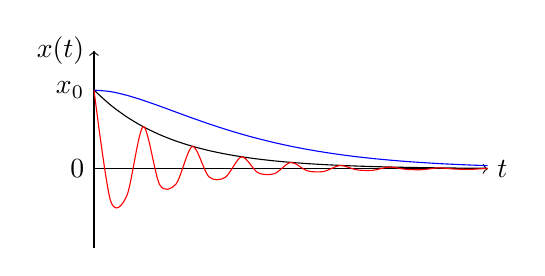
\begin{tikzpicture}
      \draw[->] (0,0) -- (5,0) node[right] {$t$};
      \draw[->] (0,-1) -- (0,1.5) node[left] {$x(t)$};
      \draw[domain=0:5,smooth,variable=\x,black] plot ({\x},{exp(-\x)});
      \draw[domain=0:5,smooth,variable=\x,blue] plot ({\x},{(1+\x)*exp(-\x)});
      \draw[domain=0:5,smooth,variable=\x,red] plot ({\x},{exp(-\x)*cos(10*\x*180/pi)});
      \draw (0,0) node[left]{0};
    \draw (0,1) node[left]{$x_0$};
\end{tikzpicture}
\end{center}
\item We want the fastest return to equilibrium, hence (b).
\item We guess a particular solution $x_p=\text{Re}[Ce^{i\Omega t}]$ where $\Omega=\frac{2\pi u}{d}$, then we have
$$\text{Re}[(-m\Omega^2+ib\Omega +k)Ce^{i\Omega t}]=\text{Re}[kAe^{i\Omega t}]\implies C=\frac{kA}{\sqrt{(k-m\Omega^2)^2+b^2\Omega^2}}e^{-i\tan^{-1}(\Omega b/(k-m\Omega^2))}$$
We thus have $$x(t)=\frac{kA}{\sqrt{(k-m\Omega^2)^2+b^2\Omega^2}}\cos\bigg(\Omega t-\tan^{-1}\bigg(\frac{\Omega b}{k-m\Omega^2}\bigg)\bigg)$$
\item To maximize the amplitude, we minimize $(k-m\Omega^2)^2+\Omega^2b^2$, which gives us either $\Omega=0$ or $\Omega^2=\frac{k}{m}-\frac{b^2}{2m^2}$. The former is trivial. We have $u=\frac{d}{2\pi}\Omega=\frac{d}{2\pi}\sqrt{(k/m)-(b^2/2m^2)}$. Hence,
$$|C|=\frac{kA}{\sqrt{(k-k+(b^2/2m))^2+(kb^2/m)-(b^4/2m^2)}}=\frac{kA}{\sqrt{(kb^2/m)-(b^4/4m)}}$$
\end{enumerate}
\end{ans}
\newpage
\begin{qns}[Dispersion]\leavevmode
\begin{enumerate}[label=(\roman*)]
\item Define phase velocity $v_p$ and group velocity $v_g$, and explain what they mean.\hfill\textbf{[4]}
\item Show that
$$v_g=v_p-\lambda\frac{dv_p}{d\lambda}$$
where $\lambda$ is the wavelength.\hfill\textbf{[4]}
\item Waves in deep water obey the dispersion relation
$$\omega^2=gk+\frac{\sigma}{\rho}k^3$$
where $g$ is the acceleration due to gravity, $\sigma$ the surface tension per unit length, and $\rho$ the water density. Show that \hfill\textbf{[6]}
$$\frac{v_g}{v_p}=1-\frac{g/k^2-\sigma/\rho}{2(g/k^2+\sigma/\rho)}$$
\item Find the wavelength $\lambda^*$ for which the ratio $v_g/v_p=1$, and comment on the nature of the wave propagation at this wavelength.\hfill\textbf{[4]}
\item Determine the value of $\lambda^*$ on a planet with a deep ocean for which $\sigma=0.11$ N m$^{-1}$, $\rho=1040$ kg m$^{-3}$, and $g = 5.0$ m s$^{-2}$.\hfill\textbf{[2]}
\end{enumerate}
\end{qns}
\begin{ans}\leavevmode
\begin{enumerate}[label=(\roman*)]
\item The phase velocity of a wave is the rate at which the phase of the wave propagates in space. This is the velocity at which the phase of any one frequency component of the wave travels. $v_p=\frac{\omega(k)}{k}$. The group velocity of a wave is the velocity with which the overall envelope shape of the wave's amplitudes—known as the modulation or envelope of the wave—propagates through space. $v_g=\frac{\partial\omega(k)}{\partial k}$ For a dispersive wave, $v_g\neq v_p$. The wave crests will move relative to the envelope.
\item With $k=\frac{2\pi}{\lambda}$,
$$v_g=\frac{d\omega}{d k}=\frac{d}{dk}(kv_p)=v_p+k\frac{dv_p}{dk}=v_p-\lambda\frac{dv_p}{d\lambda}$$
\item We have $\omega^2=gk+(\sigma/\rho)k^3\implies 2\omega\frac{d\omega}{dk}=g+3(\sigma/\rho)k^2$. Divide this by $\frac{2\omega^2}{k}$ to get
$$\frac{v_g}{v_p}=\frac{k}{\omega}\frac{d\omega}{dk}=\frac{1}{2\omega^2}(gk+3(\sigma/\rho)k^3)=\frac{(g/k^2)+(\sigma/\rho)+(2\sigma/\rho)}{2((g/k^2)+(\sigma/\rho))}=1-\frac{1}{2}+\frac{2\sigma/\rho}{2((g/k^2)+(\sigma/\rho))}$$
\item For $v_g/v_p=1$, we must have $g/k^2=\sigma/\rho$ and this gives us $\lambda=2\pi\sqrt{\sigma/g\rho}$ where we rejected the negative solution. Here, $v_g=v_p$ and there is no dispersion.
\item $\lambda^*=2\pi\sqrt{\sigma/g\rho}=2\pi\sqrt{0.11/5(1040)}=0.0289$ m.
\end{enumerate}
\end{ans}
\newpage
\begin{qns}[Fresnel Diffraction]\leavevmode
\begin{enumerate}[label=(\roman*)]
\item A plane wave of wavelength $\lambda$ is normally incident on a planar aperture with aperture function $h(x, y)$. With the aid of a diagram, show that the amplitude measured on the optic axis beyond the aperture is given by: 
$$\psi\propto\int h(x,y)K(\theta)e^{i\pi\frac{x^2+y^2}{\lambda b}}dxdy$$
explaining the assumptions you make, and explaining the meanings of $K(\theta)$ and $b$.\hfill\textbf{[6]}
\item If the aperture is a circle of radius $a$, and using the substitution $s = x^2 + y^2$, show that \hfill\textbf{[3]}
$$\psi\propto\int_0^{a^2}K(\theta)e^{i\frac{\pi s}{\lambda b}}ds$$
\item With the aid of a phasor diagram, explain the operation of a Fresnel zone plate.\hfill\textbf{[4]}
\item Calculate the outer radii of the first three open zones of a zone plate that is designed to focus x-rays of wavelength $\lambda=10$ nm at a distance of 1 m.\hfill\textbf{[3]}
\item For a zone plate of radius 0.7 mm, estimate the ratio of the intensity of light at the focus of the zone plate to the intensity at this position without the zone plate.\hfill\textbf{[4]}
\end{enumerate}
\end{qns}
\begin{ans}\leavevmode
\begin{enumerate}[label=(\roman*)]
\item Let the distance from the aperture plane's centre to the observation point be $L$, distance travelled by a light ray from a point $(x,y)$ to the origin is $r$, then 
$$r^2=L^2+x^2+y^2\implies r\approx L\bigg[1+\frac{x^2+y^2}{2L^2}+O\bigg(\bigg(\frac{x^2+y^2}{L^2}\bigg)^2\bigg)\bigg]$$
The amplitude of an infinitesimal section of light passing through a patch of size $dxdy$ at the point $h(x,y)$ is modulated by the aperture function $h(x,y)$, then traversing a distance $r$, the amplitude decays by a factor of $1/r$ and also accrues a phase $e^{ikr}$, where $k=\frac{2\pi}{\lambda}$.\\[5pt]
The scalar theory of Huygens does not account for the momentum of light and the obliquity factor $K(\theta)$ (imposed to make the rays go forward), then the infinitesimal amplitude $d\psi$ is directly proportional to $h(x,y)dxdyK(\theta)\frac{e^{ikr}}{r}$. For small apertures,
$$e^{ikr}\approx e^{i(2\pi L/\lambda)(1+\frac{x^2+y^2}{2L^2})}=e^{ikL}e^{i\pi(x^2+y^2)/\lambda L}$$
Integrating gives the total amplitude to be directly proportional to
$$\int h(x,y)K(\theta)e^{i\pi(x^2+y^2)/\lambda b}dxdy$$
where $b=L$ is the distance between the aperture plane and observation plane.
\item Let $s=x^2+y^2$, then $ds=2rdr=2dxdy$. We have $h(x,y)=1$ for $\sqrt{x^2+y^2}\leq a$ and zero otherwise. Then, the amplitude is directly proportional to
$$\int_0^{2\pi}\int_0^aK(\theta)e^{i\pi r^2/\lambda L}rdrd\phi=\pi\int_0^aK(\theta)e^{i\pi s/\lambda L}ds$$
\item The integral can be thought as addition of lots of infinitesimal length complex numbers $ds$ with a phase $\phi=\frac{\pi s}{\lambda L}$. Since $ds$ is infinitesimally small, the sequence of phasors can be approximated as an arc of a circle, with the relative phase of the last section with respect to the first to be $\frac{\pi a^2}{\lambda L}$. The phasors gradually spiral in as both factors $\frac{1}{\sqrt{s}}$ and $K$ slowly reduce the amplitude of the infinitesimal light elements reach the observation point.\\[5pt]
A zone is the region which emits light that is within $\pi$ phase with respect to the reference beam. The first zone is the region that emits between 0 and $\pi$ phase relative to the central beam, and has radius $\frac{\pi\rho_1^2}{\lambda L}<\pi\implies\rho_1<\sqrt{\lambda L}$. The second zone is the region that emit light between $\pi$ and $2\pi$ relative to the central beam, i.e. $\pi<\frac{\pi\rho^2}{\lambda L}<2\pi$. The outer edge is at $\rho_2=\sqrt{2\lambda L}$. In general, the edge of the $n$th zone is at $\sqrt{n\lambda L}$. If one were to block off alternate zones, one can achieve an intensity far beyond that of the central beam.
\item Assume we let the first three odd zones through, then $\rho_1=\sqrt{\lambda L}=0.1$ mm, $\rho_2=\sqrt{3\lambda L}=0.173$ mm and $\rho_3=\sqrt{5\lambda L}=0.224$ mm.
\item We have $\rho_n=0.7$ mm and so $n=\frac{\rho_n^2}{\lambda L}=\frac{(0.7\times10^{-3})^2}{10\times10^{-9}}=49$. The intensity is $(2\times49)^2=9604$ times as intense as when the zone plate is absent.
\end{enumerate}
\end{ans}
\begin{qns}[Michelson Interferometry]\leavevmode
\begin{enumerate}[label=(\roman*)]
\item A Michelson interferometer has two perpendicular mirrors. Draw a labelled sketch of the optical arrangement and explain how it is used.\hfill\textbf{[5]}
\item By considering a wave that is the real part of the superposition of the waves $ae^{i\omega t}$ and $ae^{i(\omega t+\phi)}$, show that the intensity measured by the Michelson detector when fed with monochromatic light of wavevector $k$ is $I(x)=I_0(1+\cos(kx))$, where $x$ is the difference in path travelled by the two beams.\hfill\textbf{[5]}
\item The light source is then changed from monochromatic to having an intensity spectrum that has a rectangular top-hat shape from $k-\Delta k/2$ to $k+\Delta k/2$. Show that the intensity measured by the Michelson detector is now \hfill\textbf{[5]}
$$I(x)\propto 1+\cos(kx)\sinc(x\Delta k/2)$$
\item Draw an annotated sketch of $I(x)$ for light with a top-hat spectrum extending from $4.95\times10^{14}$ Hz to $5.05\times10^{14}$ Hz.\hfill\textbf{[5]}
\end{enumerate}
\end{qns}
\begin{ans}\leavevmode
\begin{enumerate}[label=(\roman*)]
\item The beam-splitter splits the incident beam with components travel along different paths, and recombine at the same beam-splitter. One path is kept fixed (reference path) and the other path is varied with a movable mirror on a precision stage. A fringe pattern is obtained as a function of mirror position. The Michelson interferometer has many important applications including high precision metrology, Fourier Transform spectroscopy and the Michelson-Morley experiment.
\begin{figure}[H]
    \centering
    \includegraphics[width=\linewidth]{mmi.PNG}
    \caption{Michelson Morley Interferometer}
\end{figure}
\item With $I_0=|a|^2$,
$$I(x)=|\psi_{tot}|^2=|ae^{i\omega t}+ae^{i(\omega t+\phi)}|^2=|a|^2[1+e^{i\phi}+e^{-i\phi}+1]=2|a|^2[1+\cos(kx)]$$
\item When superposing waves of different frequencies, you must add the amplitudes and only then take the mod squared to get the resultant intensity. However, the cross-terms will have a net time dependence, which unless the frequencies are extremely close together, will time average to zero on the scale of the detectors, so we may merely superpose the intensities. Let the intensity of light in the wavenumber range $[k,k+dk]$ be $2S(k)dk$, then the total intensity observed (implicit time-averaged) will be the sum of all the sine waves weighted by the intensity at the relevant wavelength:
$$I(x)=2\int_0^\infty S(k)(1+\text{Re}[e^{ikx}])dk$$
We can also define $S(k)$ for negative $k$, such that $S(-k)=S^*(k)$, hence drop the factor of 2 and let the integration range be from $k=-\infty$ to $k=\infty$. We have
$$I(x)=\int_{-\infty}^\infty S(k)(1+e^{ikx})dk=I_1+\int_{-\infty}^\infty S(k)e^{ikx}dk$$
where $I_1=\int_{-\infty}^\infty S(k)dk$ is equal to the total intensity of the light. $S(k)$ can thus be found using inverse Fourier transform:
$$S(k)=\frac{1}{2\pi}\int_{-\infty}^\infty(I(x)-I_1)e^{-ikx}dk$$
This $S(k)$ is represented as pairs of closely-spaced delta-functions spaced about $\pm k$ convolved with a rectangular top-hat of width $\Delta k$.
$$S(k')=[\delta(k'-k)+\delta(k'+k)]*\text{Top-hat of width }\Delta k$$
Then the intensity will be
$$I(x)=I_1[1+\cos(kx)\sinc(x\Delta k/2)]$$
where the $\sinc$ is a low-frequency envelope that modulates the fringes.
\item $k=5\times10^{14}$ Hz with $\Delta k=0.1\times10^{14}$ Hz.
\end{enumerate}
\end{ans}
\newpage
\subsubsection{Section C}
\begin{qns}[Transport]\leavevmode
\begin{enumerate}[label=(\roman*)]
\item Explain the principles and approximations that form the free-electron model in metals and state what key predictions it is able to make.\hfill\textbf{[4]}
\item The equation governing the transport of electrons in an electric field is
$$m^*\frac{d\langle v\rangle}{dt}=-\gamma\langle v\rangle +eE$$
where $e$ is the electron charge, $m^*$ their effective mass, and $\tau=m^*/\gamma$ is the mean time between collision of electrons with lattice defects or phonons. Explain the origin of each term in this equation and show that the free-electron estimate for the DC electric conductivity is
$$\sigma_0=\frac{ne^2\tau}{m^*}$$
where $n$ is the number of free electrons per unit volume.\hfill\textbf{[6]}
\item Consider the case of AC current and the possible contribution of the inertial term in the equation for electron motion. Derive the corresponding frequency-dependent expression for complex electric conductivity, $\sigma(\omega)$.\hfill\textbf{[6]}
\item Sketch the plots of real and imaginary parts of $\sigma(\omega)$, and estimate the characteristic frequency at which the inertial effects become relevant.\hfill\textbf{[4]}
\end{enumerate}
\begin{mdframed}
\color{darkblue}{Metallic Cu has a free electron density $n=8.5\times10^{28}$ m$^{-3}$ and an effective mass $m^*\approx m_e$. The DC conductivity of copper is $\sigma_0=5.96\times10^7$ S m$^{-1}$.}
\end{mdframed}
\end{qns}
\begin{ans}\leavevmode
\begin{enumerate}[label=(\roman*)]
\item The free-electron model assumes that most of the electrons contributed by each atom form a `core' which is tightly bound to the nucleus, plus a few conduction electrons which disassociate to form a free electron gas. This also assumes that the net effect of all the nucleus plus core electrons is a completely uniform background positive potential that the free electrons move under. The free electrons are treated as a non-interacting gas with an effective mass $m^*$ not necessarily equal to $m_e$ (depends on interactions with the lattice). The key predictions of the free electron model are
\begin{itemize}
    \item density of states of electrons in 3D is proportional to $\sqrt{E}$ where $E$ is the energy
    \item Pauli paramagnetism of metals
    \item Wiedemann-Franz law
\end{itemize}
\item $m^*$ is the effective mass defined as $\hbar^2(\partial^2\epsilon/\partial k^2)^{-1}$. On the RHS, the second term is the net force is due to the electric field and the first term is the rate of change of momentum lost in collisions (each collision removes momentum $m^*v$ and occurs on average every $\tau$ seconds), so by Newton's second law gives
$$m^*\frac{d\langle v\rangle}{dt}=-\frac{m^*}{\tau}\langle v\rangle+eE$$
For DC, the mean speed is constant so $\langle v\rangle=\frac{\tau eE}{m^*}$. The DC electrical conductivity $\sigma$ is the current density per unit of generating DC electric field whereas the current density $J$ if the number density of electrons times the speed and charge of each electron and hence
$$\sigma=\frac{J}{E}=\frac{ne\langle v\rangle}{E}=\frac{ne^2\tau}{m^*}$$
\item In the presence of AC fields, $\frac{d\langle v\rangle}{dt}$ becomes $i\omega\langle v\rangle$, so
$$\langle v\rangle\bigg(\frac{m^*}{\tau}+i\omega m^*\bigg)=eE\implies\langle v\rangle=\frac{eE}{m^*}(i\omega+\tau^{-1})^{-1}$$
so the complex electric conductivity is
$$\sigma(\omega)=\frac{ne^2}{m^*}\frac{\tau}{1+i\omega\tau}=\frac{ne^2\tau}{m^*}\frac{1-i\omega\tau}{1+\omega^2\tau^2}$$
\item The real part of the conductivity is
$$\text{Re}[\sigma]=\frac{ne^2\tau}{m^*}\frac{1}{1+\omega^2\tau^2}$$
which is maximum at $\omega=0$ and decays to 0 with a point of inflexion at $\omega=1/\tau$, i.e.
$$0=\frac{\partial^2}{\partial\omega^2}\text{Re}[\sigma]=\frac{\partial}{\partial\omega}\bigg(\frac{-2\omega\tau^2}{(1+\omega^2\tau^2)^2}\bigg)=-\frac{2\tau^2}{(1+\omega^2\tau^2)^2}+\frac{2\omega^2\tau^4}{(1+\omega^2\tau^2)^3}\implies\omega=\tau^{-1}$$
The imaginary part of the conductivity is
$$\text{Im}[\sigma]=\frac{ne^2\tau}{m^*}\frac{-\omega\tau}{1+\omega^2\tau^2}$$
which peaks at
$$0=\frac{\partial^2}{\partial\omega^2}\text{Im}[\sigma]=\frac{-i\tau}{1+\omega^2\tau^2}+\frac{2i\omega^2\tau^3}{(1+\omega^2\tau^2)^2}=\frac{i\tau}{1+\omega^2\tau^2}[2\omega^2\tau^2-1-\omega^2\tau^2]\implies\omega=\tau^{-1}$$
The AC conductivity at this characteristic frequency $\omega=1/\tau$ is thus
$$\sigma[\omega=\tau^{-1}]=0.5\sigma_0(1-i)$$
where the real and imaginary part have the same magnitude. Below is the plot for the real and imaginary parts of $\sigma$ as the blue and red part respectively.
\begin{center}
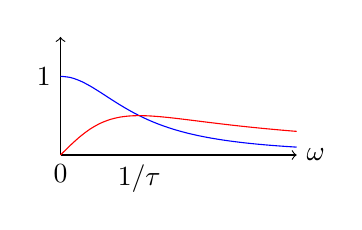
\begin{tikzpicture}
      \draw[->] (0,0) -- (3,0) node[right] {$\omega$};
      \draw[->] (0,0) -- (0,1.5) node[left] {};
      \draw[domain=0:3,smooth,variable=\x,blue] plot ({\x},{1/(1+\x^2)});
      \draw[domain=0:3,smooth,variable=\x,red] plot ({\x},{\x/(1+\x^2)});
      \draw (0,0) node[below]{0};
      \draw (1,0) node[below]{$1/\tau$};
\draw (0,1) node[left]{1};
\end{tikzpicture}
\end{center}
This characteristic frequency is
$$\omega=\frac{1}{\tau}=\frac{ne^2}{m_e\sigma_0}=\frac{(8.5\times10^{28})(1.6\times10^{-19})^2}{(9.11\times10^{-31})(5.96\times10^{-7})}=4.0\times10^{13}s^{-1}$$
\end{enumerate}
\end{ans}
\newpage
\begin{qns}[Phonons]\leavevmode
\begin{enumerate}[label=(\roman*)]
\item Consider a longitudinal wave of displacements $u_n=ue^{i(\omega t-qna)}$, which propagates in a monoatomic linear lattice of atoms of mass $M$, with spacing $a$, bonded by harmonic springs with a force constant $\alpha$. Draw a sketch of the system and show that the total energy of the wave is $E=\frac{1}{2}M\sum_n(du_n/dt)^2+\frac{1}{2}\alpha\sum(u_n-u_{n+1})^2$, where $n$ runs over all atoms.\hfill\textbf{[4]}
\item By writing down the equation of motion for an atom n, show that $\omega^2=4(\alpha/M)\sin^2(qa/2)$.

\hfill\textbf{[3]}
\item Show that the time-average total energy per atom is equal to $\frac{1}{4}M\omega^2u^2+\frac{1}{2}\alpha(1-\cos(qa))u^2=\frac{1}{2}M\omega^2u^2$.\hfill\textbf{[3]}
\item If this 1-dimensional line has a total number $N$ of equivalent atoms, show that the density of phonon states in $q$-space is $g(q)=Na/\pi$.\hfill\textbf{[3]}
\item Therefore show that the density of states $g(\omega)$ takes the form
$$g(\omega)=\frac{2N}{\pi}\frac{1}{\sqrt{\omega_m^2-\omega^2}}$$
and write down the maximum frequency $\omega_m$.\hfill\textbf{[7]}
\end{enumerate}
\end{qns}
\begin{ans}\leavevmode
\begin{enumerate}[label=(\roman*)]
\item Sketch should include a 1D chain of atoms with each spring labelled by the spring constant $\alpha$ and the displacements of the $n$th atom from their equilibrium position be $u_n$. The total energy will be the sum of the kinetic and elastic potential energies.
$$E=\sum_n\frac{1}{2}M\dot{u}_n^2+\frac{1}{2}\alpha(u_n-u_{n+1})^2$$
\item Treat the chain as classical springs and masses, then by Newton's second law, the equation of motion for the $n$th atom is
$$M\ddot{u}_n=-\alpha(u_n-u_{n+1})+\alpha(u_{n-1}-u_n)$$
As suggested in part (i), we look for normal mode solutions of the form $u_\alpha=ue^{i(\omega t-qna)}$, and hence
$$-\omega^2Mu_n=\alpha[e^{-iqa}u_n-u_n+e^{iqa}u_n-u_n]$$
which gives us the dispersion relation $\omega^2=\frac{\alpha}{M}(2-2\cos qa)=4(\alpha/M)\sin^2(aq/2)$. 
\item Let $u=|u|e^{i\phi}$, then the total kinetic energy and potential energy are respectively
$$\frac{1}{2}M\sum_n(-\omega|u|\sin(\omega t-qna+\phi))^2,\quad\frac{1}{2}\alpha|u|^2\sin^2\frac{qa}{2}\sum_n(-2\sin(\phi+\omega t+qna+0.5qna))^2$$
which gives the time-averaged $\frac{1}{4}NM\omega^2|u|^2$ and $\frac{1}{2}\alpha|u|^2N(1-\cos qa)$ respectively. Substitute the dispersion relation, the total time-averaged energy per atom is
$$\frac{\langle E\rangle}{N}=\frac{1}{4}M\omega^2|u|^2+\frac{1}{2}\alpha|u|^2(1-\cos qa)=\frac{1}{2}M\omega^2|u|^2$$
\item To fit the wave in the chain (assuming fixed boundary conditions), $u_0=u_{N-1}=0$, so the maximum wavelength is $Na/2$ (can only fit an integer number of half-wavelengths), so $m\lambda/2=Na$. $q$ is also quantized with $q=2\pi/\lambda=\pi m/Na$. The allowed states are thus equally spaced in $q$-space with density $g(q)=\frac{1}{dq/dm}=\frac{Na}{\pi}$.
\item Differentiate the dispersion relation $\omega(q)^2$:
$$2\omega\frac{d\omega}{dq}=4a\frac{\alpha}{M}\sin\frac{qa}{2}\cos\frac{qa}{2}=4a\frac{\alpha}{M}\sqrt{\frac{M\omega^2}{4\alpha}}\sqrt{1-\frac{M\omega^2}{4\alpha}}=a\omega_n^2\frac{\omega}{\omega_n}\sqrt{1-\frac{\omega^2}{\omega_n^2}}$$
where $\omega_n=2\sqrt{\alpha/M}$. Finally,
$$g(\omega)=g(q)\bigg|\frac{dq}{d\omega}\bigg|=\frac{Na}{\pi}\frac{2}{a}\frac{1}{(\omega_m^2-\omega^2)^{1/2}}$$

\end{enumerate}

\end{ans}
\newpage
\subsubsection{Section D}
\begin{qns}[CMP Essay]
Explain the concept of holes and the mechanism of hole conductivity in semiconductors, including a discussion of how the characteristics of holes can be measured experimentally and how the holes can be generated by doping.\hfill\textbf{[20]}
\end{qns}
\begin{ans}
Suppose we start with an insulator or semiconductor and we excite one electron from the valence band to the conduction band. This excitation may be due to absorption of a photon, or it might be a thermal excitation. When the electron has been moved up to the conduction band, there is an absence of an electron in the valence band known as a hole. Since a completely filled band is inert, it is very convenient to only keep track of the few holes in the valence band and to treat these holes as individual elementary particles. The electron can fall back into the empty state that is the hole, emitting energy and annihilating both the electron and hole from the conduction and valence band respectively.\\[5pt]
Using cyclotron resonances, we can measure the effective masses of `holes'. In the presence of a magnetic field $\mathbf{B}$ pointing in the positive $z$-direction, the electron feels a  Lorentz force $-e\mathbf{v}\times\mathbf{B}$ which acts to deflect electrons in the negative $y$-direction. This force is orthogonal to the velocity and will act like a centripetal force that restricts these charge particles to follow circular trajectories. As such, a charged particle in a magnetic field moves in a helix along the magnetic field axis. The period $T$ of the circular motion depends on its mass $m$ and charge $e$,
$$T=\bigg|\frac{2\pi m}{eB}\bigg|$$
For particles in asymmetrical band structures, the particle no longer moves exactly in a helix, however its motion transverse to the magnetic field still moves in a closed loop (not necessarily a circle). Moreover, the time to complete one of these loops still varies inversely with magnetic field, and so it is possible to define a cyclotron effective mass $m=m^*$ from the measured period, using the above equation.\\[5pt]
Adding dopants that gives fewer electrons than the substrate itself creates a p-type semiconductor. At non-zero temperatures, all these states are ionized, increasing the conductance of the material. For the p-type, the vast majority of the charge carriers are holes left behind when electrons from the filled band were excited into the dopant hole state. In the absence of impurities, the Fermi energy ($\mu(T=0)$) is in the middle of the band gap. When the acceptor impurities are added, at zero temperature, impurity states near the bottom of the bandgap are empty. The Fermi energy is moved down to the bottom of the band gap.
\end{ans}
\newpage
\begin{qns}[OWO Short Notes]
Write brief notes on two of the following:\hfill\textbf{[20]}
\begin{itemize}
    \item the propagation of sound waves in gases;
    \item the Q-factor and how it can be measured for free and for driven oscillators;
    \item the polarisation of transverse waves, including linear, circular and elliptical polarisation.
\end{itemize}
\end{qns}
\begin{ans}\leavevmode
\subsubsection*{The propagation of sound waves in gases:}
Recall the definition of longitudinal waves: The displacement of the medium in a longitudinal wave is in the same direction as the direction of wave propagation. Then, for a longitudinal wave in gas, we will show that the longitudinal displacement and excess pressure obey the wave equation.\\[5pt]
Let's consider a 1D wave, i.e. a tube of air inside a cylindrical container with cross-sectional area $A$. Let the ends of this section be located at $x$ and $x+\Delta x$ at equilibrium, and then at $x+\psi(x)$ and $x+\Delta x+\psi(x+\Delta x)$ at a later time. The function $\psi$ measures the longitudinal displacement from equilibrium. If we define $\Delta\psi$ to be $\psi(x+\Delta x)=\psi(x)+\Delta\psi$, where $\Delta\psi$ is how much more the right boundary of the region moves compared with the left boundary.\\[5pt]
Let the pressure in the tube at equilibrium be $p_0$. Let $\psi_p(x)$ be the excess pressure above $p_0$ as a function of $x$. The total pressure at the left boundary and the right boundary are $\psi_p(x)$ and $\psi_p(x+\Delta x)=\psi_p(x)+\Delta\psi_p$, where $\Delta\psi_p$ is how much the pressure at the right boundary exceeds the pressure at the left boundary.\\[5pt]
The change in volume from equilibrium $\Delta V=A\Delta\psi$ is directly proportional to $-V\psi_p$, where $\Delta V/V<<1$. Let the compressibility $\kappa$ be the desired constant of proportionality, then $$\frac{\partial\psi}{\partial x}=-\kappa\psi_p\implies\frac{\partial\psi_p}{\partial x}=-\frac{1}{\kappa}\frac{\partial^2\psi}{\partial x^2}$$
For ideal gas, we have isothermal compressibility be $\kappa=\frac{1}{p_0}$ and for adiabatic compressibility be $\kappa=\frac{1}{\gamma p_0}$. The net force is $F_{net}=A(p(x)-p(x+\Delta x))=A(p_0+\psi_p(x)-p_0-\psi_p(x+\Delta x))=A(-\Delta\psi_p)$ and so
$$\rho A\Delta x\frac{\partial^2\psi}{\partial t^2}=-A\bigg(-\frac{1}{\kappa}\frac{\partial^2\psi}{\partial x^2}\Delta x\bigg)\implies\frac{\partial^2\psi}{\partial t^2}=\frac{\gamma p_0}{\rho}\frac{\partial^2\psi}{\partial x^2}$$
The longitudinal displacement does satisfy the wave equation. Taking $\frac{\partial}{\partial x}$ yields $$\frac{\partial^2}{\partial t^2}\frac{\partial\psi}{\partial x}=\frac{\gamma p_0}{\rho}\frac{\partial^2}{\partial x^2}\frac{\partial\psi}{\partial x}$$
Since $\frac{\partial\psi}{\partial x}$ is directly proportional to $\psi_p$, we have the desired wave equation for excess pressure. The wave speed is $1/c=1/\sqrt{\rho/\gamma p_0}=1/\sqrt{\kappa\rho}$. The pressure leads the displacement by a phase $\pi/2$ and has amplitude $\frac{k}{\kappa}\psi$. For a harmonic wave of the form $\psi(x,t)\propto e^{i(\omega t-kx)}$, then $\psi_p(x,t)=-\frac{1}{\kappa}\frac{\partial\psi(x,t)}{\partial x}=-\frac{-ik}{\kappa}\psi(x,t)$. The excess force that a sheet of gas exerts on the region to its right is $$F=A\psi_p=A\bigg(-\frac{1}{\kappa}\frac{\partial\psi}{\partial x}\bigg)=-\frac{A}{\kappa}\bigg(\mp\frac{1}{c}\frac{\partial\psi}{\partial t}\bigg)=\frac{\pm A}{\kappa c}\frac{\partial\psi}{\partial t}$$
where we used the harmonic wave form. Hence, the acoustic impedance  $Z_{acous}$ (impedance per cross-sectional area) of the gas is $$Z_{acous}=\frac{1}{A}\frac{F}{\partial\psi/\partial t}=\frac{1}{\kappa c}=\sqrt{\rho/\kappa}=\sqrt{\gamma p_0\rho}$$
The energy density per unit volume can be shown to be $\rho(\frac{\partial\psi}{\partial t})^2$ where $A\rho=\mu$. The power on the sheet of particles whose equilibrium position is $x$ is $P=(p_0+\psi_p)A\frac{\partial\psi}{\partial t}$. Since $\psi_p=-\frac{1}{\kappa}\frac{\partial\psi}{\partial x}$, then $$P=\pm\frac{A}{\kappa c}\bigg(\frac{\partial\psi}{\partial t}\bigg)^2=\pm\frac{Ac^2\kappa^2}{\kappa c}\psi_p=\frac{c}{\rho c^2}\psi_p=\frac{\psi_p}{\rho c}$$ 
Alternatively, using the acoustic impedance $Z_{acous}=\rho c$, we have $P=\pm Z_{acous}(\frac{\partial\psi}{\partial t})^2$. The mean power per unit area, or intensity, is  $\frac{1}{2}Z_{acous}\omega^2|\psi_0|^2$. We can express the intensity of sound as a power level in decibels:
$$10\log_{10}(I/I_{ref})$$
with $I_{ref}=p_{ref}^2/Z_{acous}$ which is $10^{-12}$ W/m$^2$, where $Z_{acous}$ for air is 400 kg m$^{-2}$ s$^{-1}$.
\subsubsection*{The Q-factor and how it can be measured for free and for driven oscillators:}
For a driven oscillating system, the equation of motion is
$$\ddot{x}+\gamma\dot{x}+\omega_0^2x=f_0e^{i\omega t}$$
where $f_0$ is the driven force per unit mass. If $f_0=0$, then the oscillation is free. $\gamma$ is related to the extent of damping.\\[5pt]
Quality factor is defined to be the number of cycles for the amplitude to decrease by a factor of $e^{-\pi}$ and is the ratio of $\omega_0$ to $\gamma$. 
$$Q\equiv\frac{\omega_0}{\gamma}$$
To complete $Q$ number of cycles, the time taken can be obtained from $\omega_ut=2\pi Q$. For very light damping, $\omega_u\approx\omega_0$ and one can approximate this as $\frac{2\pi Q}{\omega_0}=\frac{2\pi}{\gamma}$ such that $e^{-0.5\gamma t}=e^{-0.5\gamma(2\pi/\gamma)}=e^{-\pi}$. Since the condition for light damping is $\gamma<2\omega_0$, $Q>0.5$. The greater the quality factor, the smaller the damping. A $Q$ factor of 0.5 corresponds to critical damping while $Q<0.5$ corresponds to heavy damping.\\[5pt]
Now, let's consider the ratio of amplitude of the $(n+1)$th peak to that of the $n$th peak, bearing in mind that the amplitudes are related by the exponential term $e^{-0.5\gamma t}$:
$$\frac{a_{n+1}}{a_n}=e^{-\gamma(t_{n+1}-t_n)}$$
The time difference between the $n$th peak and the $(n+1)$th peak is related to the period of the under-damped oscillation which is $\frac{2\pi}{\omega_u}$. We denote the quantity $\Delta$ to be the logarithmic decrement $\ln(a_{n+1}/a_n)$:
$$\Delta=\ln(e^{-\frac{1}{2}\frac{2\pi\gamma}{\omega_u}})=-\frac{\pi\gamma}{\omega_u}\approx-\frac{\pi\gamma}{\omega_0}=-\frac{\pi}{Q}$$
The number of cycles for the amplitude to fall by a factor $e$ is thus
$$\bigg|\frac{1}{\Delta}\bigg|=\frac{Q}{\pi}$$
The quality factor can thus also be defined as the number of radians of oscillations for the amplitude to fall by a factor of $e$. For free (but damped) oscillators, it is easy to measure $Q$ using the definition of logarithmic decrement in oscillation amplitude.\\[5pt]
For driven oscillators, the time-averaged power is
$$\frac{1}{2}\text{Re}[F\dot{x}^*]=\frac{1}{2}\text{Re}[i\omega mf_0Ae^{-i\phi}]=\frac{1}{2}A\omega m f_0\sin\phi=\frac{m}{2}\frac{\omega f_0^2}{\sqrt{(\omega_0^2-\omega^2)^2+\gamma^2\omega^2}}\frac{\omega\gamma}{\sqrt{(\omega_0^2-\omega^2)^2+\gamma^2\omega^2}}$$
where the phase difference between the driving force and velocity response $\phi$ satisfies $$\tan\phi=-\frac{\gamma\omega}{\omega_0^2-\omega^2}$$
The following is a sketch of time-averaged power curve as a function of driving frequency $\omega$ for different damping $\gamma$:
\begin{center}
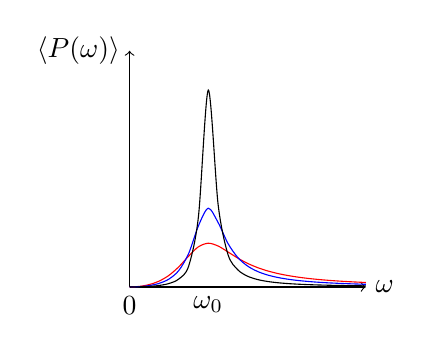
\begin{tikzpicture}
      \draw[->] (0,0) -- (3,0) node[right] {$\omega$};
      \draw[->] (0,0) -- (0,3) node[left] {$\langle P(\omega)\rangle$};
      \draw[domain=0:3,smooth,variable=\x,red] plot ({\x},{(0.9*\x^2)/(2*((1-\x^2)^2+(0.9*\x)^2))});
     \draw[domain=0:3,smooth,variable=\x,blue] plot ({\x},{(0.5*\x^2)/(2*((1-\x^2)^2+(0.5*\x)^2))});
     \draw[domain=0:3,smooth,variable=\x,black] plot ({\x},{(0.2*\x^2)/(2*((1-\x^2)^2+(0.2*\x)^2))});
     \draw (1,0) node[below]{$\omega_0$};
      \draw (0,0) node[below]{0};
\end{tikzpicture}
\end{center}
Observe, that the maximum power supplied by the driving force is during $\omega=\omega_0$. We define the full-width half maxima to be the width of the power curve (related to $|\dot{x}|^2$) at half the maximum power, then
$$\frac{\gamma^2\omega^2}{(\omega_0^2-\omega^2)^2+\gamma^2\omega^2}=\frac{1}{2}\implies(\omega_0^2-\omega^2)^2=\gamma^2\omega^2\implies\omega_0^2-\omega^2=\pm\gamma\omega\implies\Delta\omega=\gamma$$
The width of the peak thus increases when damping increases. The quality factor for driven systems, can thus be defined as $$Q=\frac{\omega_0}{\Delta\omega}$$
which is easier to measure since we only need to obtain the power spectrum of the oscillation.



\subsubsection*{The polarisation of transverse waves, including linear, circular and elliptical polarisation:}
The amplitude and relative phase along the two transverse directions (directions perpendicular to the propagation direction) will determine the polarization of transverse wave.\\[5pt]
We consider the most general polarization - elliptical polarization. There are no restriction on the amplitudes $A_z$, $A_y$ and the phase $\phi$. If however, $\phi=(m+0.5)\pi$ and $A_y=A_z$, then we obtain circular polarization. Also, if $\phi=0$ or multiples of $\pi$, then we obtain linear polarization along an intermediate direction with angle $\theta=\tan^{-1}(A_z/A_y)$. To show this, we consider generic $A_z$, $A_y$ and $\phi$,
$$\psi_z=A_z\cos(\omega t-kx+\phi)=A_z\bigg(\frac{\psi_y}{A_y}\cos\phi-\sqrt{1-\frac{\psi_y^2}{A_y^2}}\sin\phi\bigg)\implies\sin^2\phi=\frac{\psi_y^2}{A_y^2}+\frac{\psi_z^2}{A_z^2}-2\frac{\psi_y\psi_z}{A_yA_z}\cos\phi$$
with $\tan(2\alpha)=\frac{2A_yA_z\cos\phi}{A_y^2-A_z^2}$ where $\alpha$ is the angle of the major axes of the ellipse with respect to $\psi_y$. When $\phi=(m+0.5\pi)$ and $A_y=A_z$, then our equation will describe a circle, hence this is circular polarization. We define the right-circular polarization (by radio convention) to be the clockwise motion of the displacement vector when looked towards the radio source. Now if $\phi=0$ or integer multiples of $\pi$, then we obtain linear polarization, along the intermediate direction $\theta=\tan^{-1}(A_z/A_y)$ with no particular constraint on $A_z$ and $A_y$. In fact, linear polarization is obtained as a sum of two equal amplitude, coherent circularly polarized waves (one left-handed and the other right-handed).\\[5pt]
This concept is very important in electromagnetic waves which is a transverse wave with the electric field amplitude to be orthogonal to both the magnetic field amplitude and the direction of wave propagation. A solution with real $\mathbf{E_0}$, $\mathbf{B_0}$, $\mathbf{k}$ is said to be linearly polarized. If $\mathbf{E_0}$ and $\mathbf{B_0}$ are complex, then it is said to be elliptically polarized. For a circularly polarized wave, if $|\boldsymbol{\alpha}| = |\boldsymbol{\beta}|$ and $\boldsymbol{\alpha}\cdot\boldsymbol{\beta}=0$, where $\mathbf{E_0}=\boldsymbol{\alpha}+i\boldsymbol{\beta}$.
\end{ans}
\newpage
\section{2016}
\subsection{Paper 1}
\subsubsection{Section A}
\begin{qns}[Misc]
A wavepacket $\psi(x,t)$ describing a free particle at time $t=0$ is given in coordinate representation by $\psi(x,0)=1/\sqrt{a}$ for $-a/2<x<a/2$ and $\psi(x,0)=0$ for $|x|\geq a/2$. Calculate the wavefunction $\phi(p,0)$ in momentum representation and sketch its form.\hfill\textbf{[4]}
\end{qns}
\begin{ans}
Use Fourier Transform
$$\phi(p,0)=\frac{1}{\sqrt{2\pi\hbar}}\int_{-\infty}^\infty\psi(x,0)e^{-ipx/\hbar}dx=\frac{1}{\sqrt{2\pi\hbar}}\int_{-a/2}^{a/2}\frac{1}{\sqrt{a}}e^{-ipx/\hbar}dx=\frac{1}{\sqrt{2\pi a\hbar}}a\sinc\frac{pa}{2\hbar}$$
Sketch $\sinc$ curve with first zero at $p=\pm\frac{\hbar}{a}$.
\end{ans}
\begin{qns}[Scattering]
An electron beam is accelerated through a voltage of 150 V and scatters from an unknown crystalline sample. The first Bragg reflection peak is observed centred at an angle of 22\degree from the initial direction of the beam. Using Bragg's law, calculate the spacing between the Bragg planes in the sample.\hfill\textbf{[4]}
\end{qns}
\begin{ans}
Use Bragg's Law $2d\sin(\theta/2)=n\lambda$ and de Broglie relation $\sqrt{2mE}=h/\lambda$, then
$$d=\frac{hn}{2\sqrt{2mE}\sin(\theta/2)}=\frac{6.626\times10^{-34}\times 1}{2\sqrt{2(1.6\times10^{-19})(150)\sin(22\degree/2)(9.11\times10^{-31})}}=26.3 nm$$
\end{ans}
\begin{qns}[Misc]
Consider a Hermitian operator $\hat{A}$ that has the property $\hat{A}^3=\hat{I}$, where $\hat{I}$ is the identity operator. By considering the eigenvalues of $\hat{A}$, show that it must be equal to the identity operator.\hfill\textbf{[4]}
\end{qns}
\begin{ans}
Since $\hat{A}^3=\hat{I}$, then the eigenvalues $\lambda$ must satisfy $\lambda^3=I$. But the eigenvalues of a Hermitian operator must be real, and the only valid solution is $\lambda=1$. In another words, one can find a unitary matrix $U$ such that $U^\dag\hat{A}U=\diag(1,1,1)=\hat{I}$. Since $U^\dag U=\hat{I}\implies\hat{A}=\hat{I}$. 
\end{ans}
\begin{qns}[Error Analysis]
If $z=\sqrt{\tan(x)}+y^2$, with $x=(45\pm 2)\degree$ and $y=0.10\pm 0.02$, find the value of $z$ and its standard error.\hfill\textbf{[4]}
\end{qns}
\begin{ans}
We have $z=\sqrt{\tan(45\degree)}+0.10^2=1.01$. Assuming the errors are Gaussian and uncorrelated, the error in $z$ is approximately
$$\sigma_z^2\approx\bigg(\frac{\partial z}{\partial x}\bigg)^2\sigma_x^2+\bigg(\frac{\partial z}{\partial y}\bigg)^2\sigma_y^2=\bigg(\frac{\sec^2(x)}{2\sqrt{\tan(x)}}\bigg)^2\sigma_x^2+(2y)^2\sigma_y^2=\bigg(\frac{2}{2\sqrt{1}}\bigg)^2\bigg(\frac{2\pi}{180}\bigg)^2+(2\times0.10)^2(0.02^2)=1.23\times10^{-3}$$
We thus have $\sigma_z=0.035$. Hence, $z=1.01\pm0.04$.
\end{ans}
\begin{qns}[Noise]
An experiment measures a 1 nA current with a 100 kHz bandwidth. Find the r.m.s shot noise expected in the current.\hfill\textbf{[4]}
\end{qns}
\begin{ans}
The number of charges is $N=\frac{It}{e}$. Since shot noise is Poissonian, $\Delta N=\sqrt{N}$, and so the uncertainty in current is 
$$\Delta I=\frac{e}{t}\sqrt{N}=\sqrt{\frac{2Ie}{t}}=\sqrt{1.6\times10^{-19}\times2\times10^{-9}\times100\times10^3}=5.7\times10^{-12}A$$
\end{ans}
\newpage
\subsubsection{Section B}
\begin{qns}[1D Potential]
The probability current associated with the one-dimensional wavefunction $\psi(x,t)$ is given by
$$J(x,t)=\frac{\hbar}{2mi}\bigg(\psi^*\frac{\partial\psi}{\partial x}-\frac{\partial\psi^*}{\partial x}\psi\bigg)$$
where $m$ is the mass of the particle.
\begin{enumerate}[label=(\roman*)]
\item A region of space contains two superimposed plane waves propagating in opposite directions:
$$\psi=c_1e^{i(kx-\omega t)}+c_2e^{i(-kx-\omega t)}$$
where $c_1$ and $c_2$ are complex constants. Show that the net probability current is given by $J=\frac{\hbar k}{m}(|c_1|^2-|c_2|^2)$.\hfill\textbf{[5]}\\[5pt]
A particle of kinetic energy $E$ and mass $m$ is incident on a rectangular potential barrier of height $V_0=E$ that extends from $x=-a$ to $x = a$, as sketched below.
\begin{figure}[H]
    \centering
    \includegraphics[scale=0.5]{2016P1B6Q.PNG}
\end{figure}
\item Show that the wavefunction in Region 2 has the form  $\psi_2(x,t)=(bx+c)e^{-i\omega t}$ where $b$ and $c$ are complex constants.\hfill\textbf{[2]}
\item Hence show that the amplitude reflection coefficient $r$ and the amplitude transmission coefficient $\tau$ are given, respectively, by\hfill\textbf{[5]}
$$r=-\frac{ikae^{-2ika}}{1-ika}~\text{ and }~\tau=\frac{e^{-2ika}}{1-ika}$$
Thus show that the overall probability flux transmission coefficient from Region 1 to Region 3 is given by
$$T=\bigg(1+\frac{2mEa^2}{\hbar^2}\bigg)^{-1}$$
and verify that $R + T = 1$, where $R$ is the probability flux reflection coefficient.\hfill\textbf{[5]}
\item By determining the complex constants $b$ and $c$ in the wavefunction $\psi_2(x,t)$ in Region 2, calculate the probability current in this region and briefly interpret your result.\hfill\textbf{[3]}
\end{enumerate}
\end{qns}
\begin{ans}\leavevmode
\begin{enumerate}[label=(\roman*)]
\item Using the given form of $\psi$ for $J$, we have
$$\frac{\partial\psi}{\partial x}=ik(c_1e^{i(kx-\omega t)}-c_2e^{-i(kx+\omega t)})$$
$$\frac{\partial\psi^*}{\partial x}=ik(-c_1e^{-i(kx-\omega t)}+c_2e^{+i(kx+\omega t)})$$
Then, $J(x,t)=\frac{\hbar}{2mi}ik(|c_1|^2-|c_2|^2+|c_1|^2-|c_2|^2)=\frac{\hbar k}{m}(|c_1|^2-|c_2|^2)$.
\item In region 2, $V_0=E$, so $\psi(x,0)$ in region 2 satisfies $\frac{\partial^2\psi}{\partial x^2}=0\implies\psi_2(x,0)=bx+c$, where $b$ and $c$ are constants. But $\psi_2$ also satisfies the time-dependent Schrodinger equation, i.e. $i\hbar\frac{\partial\psi_2}{\partial t}=E\psi_2\implies\psi_2=e^{-iEt/\hbar}$. Thus, $\omega=\frac{E}{\hbar}=\frac{V_0}{\hbar}$.
\item We guess $\psi(x)$ to have an asymptotic form
$$\psi(x)=
\left\{
        \begin{array}{ll}
      e^{i(kx-\omega t)}+re^{-i(kx+\omega t)} & x<0\\
      (bx+c)e^{-i\omega t} & 0<x<2a\\
      \tau e^{i(kx-\omega t)} & x>2a
        \end{array}
    \right.$$ 
Let the left edge of region 1 be $x=0$. We impose continuity conditions:
\begin{itemize}
    \item Continuity of $\psi$ at $x=0$: $1+r=c$;
    \item Continuity of $\psi'$ at $x=0$: $ik(1-r)=b$;
    \item Continuity of $\psi$ at $x=2a$: $2ba+c=\tau e^{ik2a}$;
    \item Continuity of $\psi'$ at $x=2a$: $b=ik\tau e^{ik2a}$.
\end{itemize}
solving the simultaneous equations give $\tau e^{ik2a}=1-r=2ba+1+r\implies b=-\frac{r}{a}$. We then have $\frac{\tau e^{ik2a}-1}{ika}=\tau e^{ik2a}\implies\tau =\frac{e^{-2ika}}{1-ika}$ and $r=-ika\tau e^{ik2a}=\frac{-ika}{1-ika}$.
\item The transmission flux coefficient $T$ is the ratio of transmitted flux $\frac{\hbar k}{m}|\tau|^2$ to incident flux $\frac{\hbar k}{m}$. So,
$$T=|\tau|^2=\frac{1}{1+a^2k^2}=\frac{1}{1+a^2\frac{2mE}{\hbar^2}}$$
The reflection flux coefficient $R$ is the ratio of reflected flux $\frac{\hbar k}{m}|r|^2$ to incident flux.
$$R=|r|^2=\frac{k^2a^2}{1+a^2k^2}$$
such that we have $R+T=\frac{1+a^2k^2}{1+a^2k^2}=1$.
\item We have from part (iii), $b=\frac{ik}{1-ika}$ and $c=\frac{1-2ika}{1-ika}$, then
$$J_2=\frac{\hbar}{2mi}(bc^*-b^*c)=\frac{\hbar k}{m}\frac{1}{1+a^2k^2}$$
which is $T$ multiplied by the incident flux.
\end{enumerate}
\end{ans}
\newpage
\begin{qns}[Ehrenfest Theorem]
The time-dependent Schrodinger equation is
$$i\hbar\frac{\partial}{\partial t}|\psi(t)\rangle=\hat{H}|\psi(t)\rangle$$
where $\hat{H}$ is the Hamiltonian of the system under consideration.
\begin{enumerate}[label=(\roman*)]
\item For some general operator $\hat{A}$, show that the expectation value $\langle\hat{A}\rangle=\langle\psi(t)|\hat{A}|\psi(t)\rangle$ satisfies

\hfill\textbf{[4]}
$$\frac{d\langle\hat{A}\rangle}{dt}=\frac{i}{\hbar}\langle[\hat{H},\hat{A}]\rangle+\bigg\langle\frac{d\hat{A}}{dt}\bigg\rangle$$
\item For general operators $\hat{A}$, $\hat{B}$ and $\hat{C}$ , show that $[\hat{A},\hat{B}\hat{C}]=[\hat{A},\hat{B}]\hat{C}+\hat{B}[\hat{A},\hat{C}]$, where the commutator $[\hat{A},\hat{B}]=\hat{A}\hat{B}-\hat{B}\hat{A}$.\hfill\textbf{[2]}
\item Suppose that the operators $\hat{A}$ and $\hat{B}$ each commute with their commutator $[\hat{A},\hat{B}]$. If the relationship $[\hat{A}^n,\hat{B}]=n[\hat{A},\hat{B}]\hat{A}^{n-1}$ holds for some positive integer $n = m$, show that it also holds for $n = m + 1$ and hence that it holds where $n$ is any positive integer.\hfill\textbf{[5]}
\item Hence show that for any function $F(x)$ that can be expanded as a power series in $x$, such that $F(x)=\sum_{n=0}^\infty a_nx^n$, one has $[F(\hat{A}),\hat{B}]=[\hat{A},\hat{B}]F'(\hat{A})$, where $F'(x)$ denotes the derivative $\frac{dF}{dx}$.\hfill\textbf{[3]}
\item For a system described by the time-independent Hamiltonian $\hat{H}=\hat{p}^2/(2m)+V(\hat{x})$, where $V(x)$ can be expanded as a power series in $x$, show that
$$\frac{d\langle\hat{x}\rangle}{dt}=\frac{\langle\hat{p}\rangle}{m}~\text{ and }~\frac{d\langle\hat{p}\rangle}{dt}=-\bigg\langle\frac{dV(\hat{x})}{d\hat{x}}\bigg\rangle$$
and comment briefly on the physical significance of these results.\hfill\textbf{[6]}
\end{enumerate}
\end{qns}
\begin{ans}\leavevmode
\begin{enumerate}[label=(\roman*)]
\item Using Schrodinger Equation $i\hbar\frac{\partial}{\partial t}|\psi(t)\rangle=\hat{H}|\psi(t)\rangle$, 
$$\frac{d}{dt}\langle\hat{A}\rangle=\frac{1}{-i\hbar}\langle\psi(t)|\hat{H}\hat{A}|\psi(t)\rangle+\langle\psi(t)|\hat{A}\hat{H}|\psi(t)\rangle\frac{1}{i\hbar}+\bigg\langle\frac{d\hat{A}}{dt}\bigg\rangle=\frac{-1}{i\hbar}\langle[\hat{H},\hat{A}]\rangle+\bigg\langle\frac{d\hat{A}}{dt}\bigg\rangle$$
\item $[\hat{A},\hat{B}\hat{C}]=\hat{A}\hat{B}\hat{C}-\hat{B}\hat{A}\hat{C}+\hat{B}\hat{A}\hat{C}-\hat{B}\hat{C}\hat{A}=[\hat{A},\hat{B}]\hat{C}+\hat{B}[\hat{A},\hat{C}]$.
\item We prove this by induction. Suppose the statement is true for some $m\in\mathbb{Z}^+$, then check $m+1$ case. We use the result from part (ii)
$$[\hat{A}^{m+1},\hat{B}]=\hat{A}[\hat{A}^m,\hat{B}]+[\hat{A},\hat{B}]\hat{A}^m=\hat{A}m\hat{A}^{m-1}[\hat{A},\hat{B}]+[\hat{A},\hat{B}]\hat{A}^m=(m+1)\hat{A}^m[\hat{A},\hat{B}]$$
\item Using result from part(iii), $[F(\hat{A}),\hat{B}]=\sum_{n=0}^\infty a_n[\hat{A}^n,\hat{B}]=\sum_{n=0}^\infty a_nn[\hat{A},\hat{B}]\hat{A}^{n-1}=F'(\hat{A})[\hat{A},\hat{B}]$.
\item From part(i),
$$\frac{d\langle\hat{x}\rangle}{dt}=\frac{i}{\hbar}\langle[\frac{\hat{p}^2}{2m},\hat{x}]\rangle+0=\frac{2i}{\hbar2m}\langle[\hat{p},\hat{x}],\hat{p}\rangle=\frac{i}{\hbar m}\langle(-i\hbar)\hat{p}\rangle=\frac{\langle\hat{p}\rangle}{m}$$
$$\frac{d\langle\hat{p}\rangle}{dt}=\frac{i}{\hbar}\langle[V(\hat{x}),\hat{p}]\rangle+0=\frac{i}{\hbar}\bigg\langle\frac{\partial V(\hat{x})}{\partial\hat{x}}[\hat{x},\hat{p}]\bigg\rangle-\bigg\langle\frac{dV(\hat{x})}{d\hat{x}}\bigg\rangle$$
where we used the result from part (iii) and (iv) respectively. For the former, the expectation of $\hat{p}$ behaves like the classical counterpart, while the latter looks like Newton's Second Law. In the classical limit, we have $\langle V'(\hat{x})\rangle=V'(\langle\hat{x}\rangle)$, in accordance to the correspondence principle.
\end{enumerate}
\end{ans}
\newpage
\begin{qns}[Angular Momentum]
The operators for the components of orbital angular momentum satisfy the commutation relations $[\hat{L}_x,\hat{L}_y]=i\hbar\hat{L}_z$, $[\hat{L}_y,\hat{L}_z]=i\hbar\hat{L}_x$, $[\hat{L}_z,\hat{L}_x]=i\hbar\hat{L}_y$, and the operator $\hat{L}^2=\hat{L}_x^2+\hat{L}_y^2+\hat{L}_z^2$ commutes with $\hat{L}_x$, $\hat{L}_y$ and $\hat{L}_z$.
\begin{enumerate}[label=(\roman*)]
\item For the operators $\hat{L}_\pm=\hat{L}_x\pm i\hat{L}_y$, show that\hfill\textbf{[4]} 
$$[\hat{L}_z,\hat{L}_\pm]=\pm\hbar\hat{L}_\pm~\text{ and }~\hat{L}_-\hat{L}_+=\hat{L}^2-\hat{L}_z^2-\hbar\hat{L}_z$$
\item If $|\psi\rangle$ is an eigenstate of $\hat{L}_z$ having eigenvalue $\alpha\hbar$, where $\alpha$ is a real number, show that $\hat{L}_+|\psi\rangle$ and $\hat{L}_-|\psi\rangle$ are also eigenstates of $\hat{L}_z$ having eigenvalues $(\alpha + 1)\hbar$ and $(\alpha-1)\hbar$ respectively.

\hfill\textbf{[2]}
\item If $|\psi\rangle$ is also an eigenstate of $\hat{L}^2$ having eigenvalue $\Lambda\hbar^2$, where $\Lambda$ is a real number, show that $\hat{L}_+|\psi\rangle$ and $\hat{L}_-|\psi\rangle$ are also eigenstates of $\hat{L}^2$ having eigenvalue $\Lambda\hbar^2$. \hfill\textbf{[2]}
\item By considering the form of $\hat{L}_z$ in spherical polar coordinates, or otherwise, explain why $\alpha$ must be an integer and hence show that
$$\hat{L}^2|l,m_l\rangle=l(l+1)\hbar^2|l,m_l\rangle~\text{ and }~\hat{L}_z|l,m_l\rangle=m_l\hbar|l,m_l\rangle$$
where $l$ is an integer and $m_l\in[-l,-l+1,...,1,0,1,...,l-1,l]$.\hfill\textbf{[6]}
\item Consider a particle with wavefunction
$$\psi(x,y,z)=A(x+y+z)e^{-(x^2+y^2+z^2)/a^2}$$
where $A$ is a normalisation constant and $a$ is a real parameter. Find the probability that a simultaneous measurement of $L^2$ and $L_z$ yields the values $2\hbar^2$ and $\hbar$, respectively.\hfill\textbf{[6]}
\end{enumerate}
\begin{mdframed}
\color{darkblue}{You may assume that the wavefunctions corresponding to the eigenstates $|l,m_l\rangle$ are the spherical harmonics $Y_{l,m_l}(\theta,\phi)$ and that $Y_{1,0}=\sqrt{\frac{3}{4\pi}}\cos\theta$ and $Y_{1,\pm1}=\mp\sqrt{\frac{3}{8\pi}}\sin\theta e^{\pm i\phi}$.}
\end{mdframed}
\end{qns}
\newpage
\begin{ans}\leavevmode
\begin{enumerate}[label=(\roman*)]
\item $[\hat{L}_z,\hat{L}_\pm]=[\hat{L}_z,\hat{L}_x]\pm i[\hat{L}_z,\hat{L}_y]=i\hbar\hat{L}_y\pm i(-i\hbar\hat{L}_x)=\pm\hbar\hat{L}_\pm$ and
$$\hat{L}_-\hat{L}_+=(\hat{L}_x-i\hat{L}_y)(\hat{L}_x+i\hat{L}_y)=\hat{L}_x^2+\hat{L}_y^2+i[\hat{L}_x,\hat{L}_y]=\hat{L}^2-\hat{L}_z^2-\hbar\hat{L}_z$$
\item Using result from part (i):
$$\hat{L}_z(\hat{L}_\pm|\psi\rangle)=(\pm\hbar\hat{L}_\pm+\hat{L}_\pm\hat{L}_z)|\psi\rangle=\pm\hbar\hat{L}_\pm|\psi\rangle+\alpha\hbar\hat{L}_\pm|\psi\rangle=(\alpha\pm1)\hbar\hat{L}_\pm|\psi\rangle$$
\item Given $\hat{L}^2$ commutes with $\hat{L}_x$ and $\hat{L}_y$, then by linearity, $\hat{L}^2$ commutes with $\hat{L}_\pm$.
$$\hat{L}^2\hat{L}_\pm|\psi\rangle=\hat{L}_\pm\hat{L}^2|\psi\rangle=\hat{L}_\pm\Lambda\hbar^2|\psi\rangle$$
\item $\hat{L}_z=\frac{\hbar}{i}\frac{\partial}{\partial\phi}$ and so the eigenstates $\psi\propto e^{i\alpha\phi}$. But $\psi$ must be single-valued, i.e. $\psi(\phi+2\pi)=\psi(\phi)\implies\alpha\in\mathbb{Z}$. We denote this as $m_l$ such that $\hat{L}_z|l,m_l\rangle=m_l\hbar|l,m_l\rangle$. Since $\hat{L}^2=\hat{L}_x^2+\hat{L}_y^2+\hat{L}_z^2\geq\hat{L}_z^2$, then if $\psi$ is a common eigenstate, then $\Lambda\geq\alpha^2$. This would mean there exists a state that is annihilated by $\hat{L}_+$. Label this state as $|\Lambda,l\rangle$. From the result of part (i),
$$\hat{L}^2|\Lambda,l\rangle=\hat{L}_-\hat{L}_+|\Lambda,l\rangle+\hat{L}_z^2|\Lambda,l\rangle+\hbar\hat{L}_z|\Lambda,l\rangle\implies\hbar^2\Lambda|\Lambda,l\rangle=0+\hbar^2l^2|\Lambda,l\rangle+\hbar^2l|\Lambda,l\rangle$$
which gives $\Lambda=l^2+l=l(l+1)$. By symmetry, there exists another state annihilated by $\hat{L}_-$. Label this as $|\Lambda,-l\rangle$, and we can similarly show $\Lambda=l^2-l=-l(-l+1)$, hence $m_l\in\{-l,-l+1,...,-1,0,1,...,l-1,l\}$.
\item In spherical coordinates, $\psi(\rho,\theta,\phi)=A\rho e^{-\rho^2/a^2}(\sin\theta\cos\phi+\sin\theta\sin\phi+\cos\theta)$. Only the angular components matter. We define the normalization constant $B$ such that
$$|B|^2\int_0^\pi\int_0^{2\pi}(\sin\theta+\sin\theta\sin\phi+\cos\theta)^2\sin\theta d\theta d\phi=1$$
Observe that from the orthogonality of trigonometric functions, we can eliminate many terms and eventually get $|B|=\frac{1}{\sqrt{4\pi}}$. For $\hat{L}^2$ to yield $2\hbar^2\implies l=1$, and $\hat{L}_z$ to yield $\hbar\implies m_l=1$, we must have $Y_{1,1}$ (which is $-\sqrt{\frac{3}{8\pi}}\sin\theta e^{\pm i\phi}$. The probability of that is
\begin{eqnarray}
P(L^2=2\hbar^2,L_z=\hbar)&=&
\bigg|\int_0^\pi\int_0^{2\pi}\sqrt{\frac{3}{8\pi}}\frac{1}{\sqrt{4\pi}}\sin\theta e^{\pm i\phi}(\sin\theta\cos\phi+\sin\theta\sin\phi+\cos\theta)\sin\theta d\phi d\theta\bigg|^2\nonumber\\&=&\frac{3}{8\pi}\frac{1}{4\pi}\bigg|\int_0^\pi\int_0^{2\pi}(\cos\phi\pm i\sin\phi)(\sin^3\theta\cos\phi+\sin^3\theta\sin\phi+\cos\theta\sin^2\theta)d\phi d\theta\bigg|^2\nonumber\\&=&\frac{3}{8\pi}\frac{1}{4\pi}\bigg|\int_0^\pi\sin^3\theta d\theta\int_0^{2\pi}(\cos^2\phi\pm i\sin^2\phi)d\phi\bigg|^2\nonumber\\&=&\frac{3}{32\pi^2}\frac{4^2}{3^2}\pi^2(1^2+1^2)\nonumber\\&=&\frac{1}{3}\nonumber
\end{eqnarray}
where we exploited orthogonality again to simplify the nasty integral.
\end{enumerate}
\end{ans}
\newpage
\begin{qns}[Spin]
For a particle with spin $s=\frac{1}{2}$ the operators $\hat{S}_x$, $\hat{S}_y$ and $\hat{S}_z$ for the spin components along the $x$-, $y$- and $z$-directions, respectively, may be represented by the matrices
$$S_x=\frac{\hbar}{2}\begin{pmatrix}0&1\\1&0\\\end{pmatrix},\quad S_y=\frac{\hbar}{2}\begin{pmatrix}0&-i\\i&0\\\end{pmatrix},\quad S_z=\frac{\hbar}{2}\begin{pmatrix}1&0\\0&-1\\\end{pmatrix}$$
\begin{enumerate}[label=(\roman*)]
\item Denoting the eigenstates of $\hat{S}_z$ by $|\uparrow\rangle=(1,0)^T$ and $|\downarrow\rangle=(0,1)^T$, calculate $\hat{S}_j|\uparrow\rangle$ and $\hat{S}_j|\downarrow\rangle$ for $j = x$, $y$, $z$ and determine the eigenstates of $\hat{S}_x$ and $\hat{S}_y$.\hfill\textbf{[5]}
\item For a particle in the state $|\chi\rangle=a|\uparrow\rangle+b|\downarrow\rangle$, where $a$ and $b$ are complex numbers, calculate $\langle\hat{S}_z\rangle$  and $\langle\hat{S}^2\rangle$, where $\hat{S}^2=\hat{S}_x^2+\hat{S}_y^2+\hat{S}_z^2$.\hfill\textbf{[5]}
\item Suppose one measures the component of spin along some other axis $z'$, inclined at an angle $\theta$ to the original $z$-axis, such that $\hat{S}_{z'}=\hat{S}_x\sin\theta+\hat{S}_z\cos\theta$. Calculate the eigenvalues and eigenstates of $\hat{S}_{z'}$.\hfill\textbf{[5]}
\item If a particle is in the state $|\uparrow\rangle$ referred to the $z$-axis, calculate the probabilities that a spin measurement along the $z'$-axis will yield the values $\hbar/2$ or $-\hbar/2$ respectively.\hfill\textbf{[3]}
\item What is the expectation value of a spin measurement along the $z'$-axis?\hfill\textbf{[2]}
\end{enumerate}
\end{qns}
\begin{ans}\leavevmode
\begin{enumerate}[label=(\roman*)]
\item Denote $|\uparrow\rangle$ as $|+\rangle$ and $|\downarrow\rangle$ as $|-\rangle$ instead, then
$$\hat{S}_z|\pm\rangle=\pm\frac{\hbar}{2}|\pm\rangle; \quad\hat{S}_x|\pm\rangle=\frac{\hbar}{2}|\mp\rangle;\quad\hat{S}_y=\pm i\frac{\hbar}{2}|\mp\rangle$$
By inspection, we realize that $\frac{1}{\sqrt{2}}(|+\rangle\pm|-\rangle)$ and $\frac{1}{\sqrt{2}}(|+\rangle\pm i|-\rangle)$ are the normalized eigenstates of $\hat{S}_x$ and $\hat{S}_y$ respectively.
\item From the result of (i), we realize
\begin{itemize}
    \item $\langle\hat{S}_z\rangle=\frac{\hbar}{2}(|a|^2-|b|^2)$;
    \item $\langle\hat{S}_x^2\rangle=\langle\hat{S}_y^2\rangle=\langle\hat{S}_z^2\rangle=\frac{\hbar}{4}(|a|^2+|b|^2)$ and thus $\langle S^2\rangle=\frac{3\hbar^2}{4}(|a|^2+|b|^2)$;
\end{itemize}
\item We solve:
$$0=\det(\hat{S}_{z'}-\lambda I)=\begin{vmatrix}\cos\theta-\lambda&\sin\theta\\\sin\theta&-\cos\theta-\lambda\\\end{vmatrix}=-(\cos\theta-\lambda)(\cos\theta+\lambda)-\sin^2\theta=\lambda^2-1\implies\lambda=\pm1$$
Let the eigenvector be $(a,b)^T$. Then, $\lambda=\pm1$ gives $(\cos\theta\mp1)a+\sin\theta b=0$ and $\sin\theta a-(\cos\theta\pm 1)b=0$, which have solutions $a=\cos\theta+1=2\cos^2\frac{\theta}{2}$ and $b=\sin\theta=2\sin\frac{\theta}{2}\cos\frac{\theta}{2}$. In this case, the normalized eigenvectors are $(\sin\frac{\theta}{2},\pm\cos\frac{\theta}{2})$ with corresponding eigenvalues $\pm\frac{\hbar}{2}$.
\item The probability is
$$P(+0.5\hbar)=\bigg|\begin{pmatrix}1\\0\\\end{pmatrix}\cdot\begin{pmatrix}\cos\frac{\theta}{2}\\\sin\frac{\theta}{2}\\\end{pmatrix}\bigg|^2=\cos^2\frac{\theta}{2}$$
$$P(-0.5\hbar)=\bigg|\begin{pmatrix}0\\1\\\end{pmatrix}\cdot\begin{pmatrix}\cos\frac{\theta}{2}\\\sin\frac{\theta}{2}\\\end{pmatrix}\bigg|^2=\sin^2\frac{\theta}{2}$$
\item Hence, the expectation is
$$\langle\hat{S}_{z'}\rangle=\frac{\hbar}{2}\cos^2\frac{\theta}{2}+(-0.5\hbar)\sin^2\frac{\theta}{2}=\frac{\hbar}{2}\cos\theta$$
\end{enumerate}
\end{ans}
\newpage
\subsubsection{Section C}
\begin{qns}[QM Essay]
Write an essay on systems of identical particles in quantum mechanics.\hfill\textbf{[20]}
\end{qns}
\begin{ans}
In classical mechanics, when a system is made of identical particles, it is possible to identify and distinguish each particle from the others. In quantum mechanics, however, identical particles are truly indistinguishable since we cannot specify more than a complete set of commuting observables, and due to uncertainty principle (path of a particle is meaningless).\\[5pt]
As an example, when scattering two identical particles in the centre of mass frame, it is impossible to forecast with certitude that the particle fired from source $S_1$ will make it to detector 1 or 2. 
\begin{figure}[H]
    \centering
    \includegraphics[width=\linewidth]{indistinguishable.PNG}
    \caption{Scattering of Indistinguishable Particles}
\end{figure}
Consider two particles with single particle basis $|\alpha\rangle$ and $|\beta\rangle$ respectively. We define the transposition operator
$$P_{12}|\alpha\rangle|\beta\rangle:=|\beta\rangle|\alpha\rangle$$
where $|\alpha\rangle|\beta\rangle=|\alpha\rangle\otimes|\beta\rangle$. Note $P_{12}\in\mathcal{L}(V\otimes V)$. The transposition operator is Hermitian, i.e. $P_{12}^\dag=P_{12}$. The eigenvalues of $P_{12}$ are $\pm1$, where $+1$ represents symmetric states and $-1$ represents anti-symmetric states.\\[5pt]
The spin-statistics theorem states that particles whose spin is an integer (half odd integer) multiple of $\hbar$ are described by totally symmetrical (anti-symmetric) states. They are bosons (fermions) and satisfy the Bose-Einstein (Fermi-Dirac statistics). Moreover, partially symmetric states do not exist. Essentially, for a system of $N$ identical particles,
$$P_{ij}|N\text{ identical bosons }\rangle=+|N\text{ identical bosons }\rangle$$
$$P_{ij}|N\text{ identical fermions }\rangle=-|N\text{ identical fermions}\rangle$$
where $P_{ij}$ is the permutation operator that interchanges the $i$th and the $j$ th particles, with $i$ and $j$ arbitrary.\\[5pt]
Consider two particles with states they can occupy be $|\alpha\rangle$ and $|\beta\rangle$. For bosons, the independent states are
$$|\alpha\rangle|\alpha\rangle,\quad|\beta\rangle|\beta\rangle,\quad\frac{1}{\sqrt{2}}(|\alpha\rangle|\beta\rangle+|\beta\rangle|\alpha\rangle)$$
For fermions, the only independent state can be written as
$$\frac{1}{\sqrt{2}}(|\alpha\rangle|\beta\rangle-|\beta\rangle|\alpha\rangle)$$
For classical particles (distinguishable), they follow the Maxwell-Boltzmann statistics. the independent states are $|\alpha\rangle|\beta\rangle$, $|\beta\rangle|\alpha\rangle$, $|\alpha\rangle|\alpha\rangle$, $|\beta\rangle|\beta\rangle$.\\[5pt]
For any two fermions, say if $\alpha=\beta$, the state vanishes, i.e. no such state exists. This is called Pauli Exclusion Principle, which states that no two fermions can occupy the same state.\\[5pt]
We generalize this to $N$ identical particles. For a system of many identical particles, we can define
$$P_{ij}|k^1\rangle|k^2\rangle...|k^i\rangle|k^{i+1}\rangle...|k^j\rangle...:=|k^1\rangle|k^2\rangle...|k^j\rangle|k^{i+1}\rangle...|k^i\rangle...$$
It is clear that $P_{ij}^2=1$ and the allowed eigenvalues are $\pm 1$ as well. Also, $[P_{ij},P_{kl}]\neq 0$. The normalization is $\sqrt{\prod_{i=1}^nN_i!/N!}$ where $N$ is the total number of particles and $N_i$ is the number of times $|k^{(i)}\rangle$ occurs. For $N$ particle systems, we can define $N!$ permutation operators. To build an anti-symmetric $N$ particle states, we use the Slater determinant (determinant ensures exchange of any two particles will give a minus sign).\\[5pt]
The total wavefunction may be written as a product of spatial $\psi(\mathbf{r_i})$ and spin wavefunction $\chi(\mathbf{m_{s_i}})$. We denote it as $|\Psi\rangle\in V\otimes W$, where $V$ and $W$ are spaces for spatial and spin states respectively. The overall state must satisfy the symmetrization postulate. Say if the overall state must be antisymmetric, then either spatial or the spin state must be symmetric, with the other being antisymmetric.
\end{ans}
\newpage
\begin{qns}[QM Short Notes]
Write brief notes on two of the following:\hfill\textbf{[20]}
\begin{itemize}
    \item electron wavefunctions in the hydrogen atom;
    \item experimental evidence for quantum tunnelling;
    \item creation and annihilation (ladder) operators for the harmonic oscillator.
\end{itemize}
\end{qns}
\begin{ans}\leavevmode
\subsubsection*{Electron wavefunctions in the Hydrogen atom:}
The Schr\"{o}dinger's equation in spherical coordinates is
$$\mathbf{\hat{H}}(r)=\frac{-\hbar^2}{2m}\mathbf{\hat{p}}_r^2+\frac{\mathbf{\hat{L}^2}}{2mr^2}+V(r,\theta,\phi)$$
where the radial momentum is
$$\mathbf{\hat{p}_r}=\frac{1}{2}\bigg(\frac{\mathbf{\hat{r}}}{r}\cdot\mathbf{\hat{p}}+\mathbf{\hat{p}}\cdot\frac{\mathbf{\hat{r}}}{r}\bigg)=\frac{\hbar}{2i}\bigg(2\frac{\partial}{\partial r}+\frac{1}{r^2}\frac{\partial}{\partial r}r^2\bigg)=-i\hbar\frac{1}{r}\frac{\partial}{\partial r}r$$
The operator $\mathbf{\hat{L}^2}$ appears in the del operator $\nabla$:
$$\nabla^2=\frac{1}{r^2}\frac{\partial}{\partial r}\bigg(r^2\frac{\partial}{\partial r}\bigg)-\frac{\mathbf{\hat{L}}^2}{\hbar^2r^2}=\frac{1}{r}\frac{\partial^2}{\partial r^2}r-\frac{\mathbf{\hat{L}^2}}{\hbar^2r^2}$$
A central potential, $V(r)$ is spherically symmetric about the origin. The Coulomb potential  $V(r)=-\frac{e^2}{4\pi\epsilon_0r}$ is an example of a central potential. Using the separation of variables $\psi(r,\theta,\phi)=R(r)Y_{l,m}(\theta,\phi)$, the corresponding 1D radial Schr\"{o}dinger Equation is
$$-\frac{\hbar^2}{2m}\bigg(\frac{d^2R(r)}{dr^2}+\frac{2}{r}\frac{dR(r)}{dr}\bigg)+\bigg(\frac{\hbar^2}{2mr^2}l(l+1)+\frac{e^2}{4\pi\epsilon_0r}\bigg)R(r)=ER(r)$$
Upon a further substitution of $\gamma(r)=rR(r)$, the radial part becomes
$$-\frac{d^2\gamma}{dr^2}+\frac{l(l+1)}{r^2}\gamma+\frac{2m}{\hbar^2}\bigg(\frac{e^2}{4\pi\epsilon_0r}-E\bigg)\gamma=0$$
We skip the derivation and merely quote the solution. The full normalized wavefunction for our Hydrogen atom is
$$\psi_{n,l,m}(r,\theta,\phi)
=-\bigg(\frac{2}{na_0}\bigg)^{1.5}\sqrt{\frac{(n-l-1)!}{2n(n+1)!}}\bigg(\frac{2r}{na_0}\bigg)^le^{-r/(na_0)}L_{n-l-1}^{2l+1}\bigg(\frac{2r}{na_0}\bigg)Y_{m,l}(\theta,\phi)$$
where the associated Laguerre polynomials have the form
$$L_k^N(r)=\frac{e^rr^{-N}}{k!}\frac{d^k}{dr^k}(e^{-r}r^{k+N})$$
The radial wavefunction has $n-l-1$ radial nodes since $L_{n-l-1}^{2l+1}$ has degree $n-l-1$. The number $l$ varies from 0 to $n-1$ and $m$ can take $2l+1$ values so the degeneracy of the bound states of the Hydrogen atom is
$$g_n=\sum_{l=0}^{n-1}2l+1=n^2$$
The degeneracy with respect to $l$ is a feature of the $1/r$ Coulomb potential. For more general central potentials for multi-electron atoms, the energy eigenvalues depend on both $n$ and $l$. The degeneracy with respect to $m_l$ is a consequence of rotational symmetry. These wavefunctions have a radial and angular part, where the radial part determines the radial probability distribution of the electrons, while the angular part dictates the shape of the orbitals in 3D space.\\[5pt]
Consider the example of $n=1$. For the ground state, there is only one possible value for $l$ and $m$ which are both zero. The wavefunction have no angular dependence, i.e. $Y_{m,l}(\theta,\phi)=$constant, and will just appear as a sphere in 3D. The radial probability distribution $r^2|R(r)|^2$ peaks at $r=a_0$, followed by an exponential decay. We call this orbital - the 1s orbital.
$$\psi_{1,0,0}(r,\theta,\phi)=-\bigg(\frac{2}{a_0}\bigg)^{3/2}\sqrt{\frac{1}{2}}e^{-r/(a_0)}L_{0}^{1}(2r/(a_0))Y_0^0(\theta,\phi)=-\bigg(\frac{2}{a_0}\bigg)^{3/2}\sqrt{\frac{1}{2}}e^{-r/(a_0)}\frac{1}{2\sqrt{\pi}}$$
The norm is $|\psi_{1,0,0}(r)|^2\propto e^{-2r/a_0}$. Consider the example of $n=2$. For the first excited state, there is two possible values for $l$ which are 1 and 0. First consider the latter, where it has no angular dependence. This will be a spherical orbital and it is called the 2s orbital. The radial probability distribution shows two peaks and a node at $r=2a_0$. $\psi_{2,0,0}(r,\theta,\phi)$ is
$$-\bigg(\frac{2}{2a_0}\bigg)^{3/2}\sqrt{\frac{1}{2(2)(2!)}}e^{-r/(2a_0)}L_{1}^{1}(2r/(2a_0))Y_0^0(\theta,\phi)=-\bigg(\frac{2}{2a_0}\bigg)^{3/2}\sqrt{\frac{1}{2(2)(2!)}}e^{-r/(2a_0)}\bigg(2-\frac{2r}{2a_0}\bigg)\frac{1}{2\sqrt{\pi}}$$
The norm is $|\psi_{2,0,0}(r)|^2\propto e^{-r/a_0}(2-ra_0^{-1})^2$. For the former, there are 3 possible values of $m$ and corresponds to three 2p orbitals which appear as lobe-shaped dumbbells and are oriented in the three distinct directions. The wavefunctions for $m=0$ and $m=\pm1$ respectively are
$$-\bigg(\frac{2}{2a_0}\bigg)^{3/2}\sqrt{\frac{1}{2(2)(3!)}}\bigg(\frac{2r}{2a_0}\bigg)e^{-r/(2a_0)}L_{0}^{3}(2r/(a_0))Y_1^0(\theta,\phi)=-\bigg(\frac{1}{a_0}\bigg)^{3/2}\frac{1}{\sqrt{24}}\bigg(\frac{r}{a_0}\bigg)e^{-r/(2a_0)}\frac{1}{2}\sqrt{\frac{3}{\pi}}\cos(\theta)$$
$$-\bigg(\frac{2}{2a_0}\bigg)^{3/2}\sqrt{\frac{1}{2(2)(3!)}}\bigg(\frac{2r}{2a_0}\bigg)e^{-r/(2a_0)}L_{0}^{3}(2r/(a_0))Y_1^{\pm1}(\theta,\phi)=\pm\bigg(\frac{1}{a_0}\bigg)^{3/2}\frac{1}{\sqrt{24}}\bigg(\frac{r}{a_0}\bigg)e^{-r/(2a_0)}\frac{1}{2}\sqrt{\frac{3}{2\pi}}e^{\pm i\phi}\sin(\theta)$$
The norms are respectively  $|\psi_{2,1,0}(r,\theta)|^2\propto r^2e^{-r/a_0}\cos^2\theta$ and $|\psi_{2,1,\pm1}(r,\theta)|^2\propto r^2e^{-r/a_0}\sin^2\theta$, where the $\phi$ dependence (appear as a phase) disappear in the latter's norm. Below we plot the radial distribution function $|R(r)|^2r^2$ for 1s (black), 2s (red) and 2p (blue) orbitals:
\begin{center}
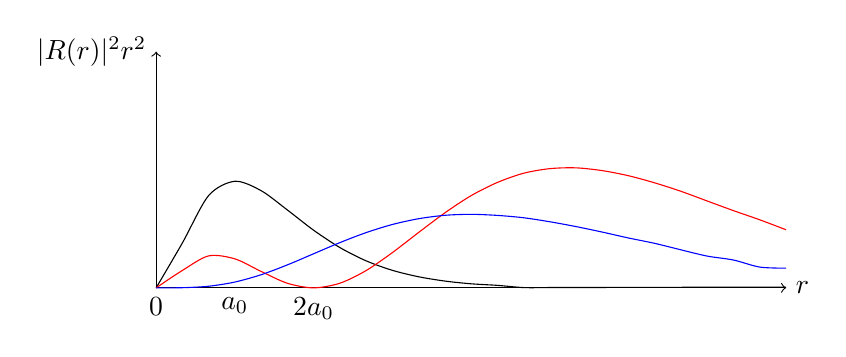
\begin{tikzpicture}
      \draw[->] (0,0) -- (8,0) node[right] {$r$};
      \draw[->] (0,0) -- (0,3) node[left] {$|R(r)|^2r^2$};
      \draw[domain=0:8,smooth,variable=\x,black] plot ({\x},{10*\x^2*exp(-2*\x)});
      \draw[domain=0:8,smooth,variable=\x,red] plot ({\x},{\x^2*exp(-\x)*(2-\x)^2});
      \draw[domain=0:8,smooth,variable=\x,blue] plot ({\x},{0.2*exp(-\x)*\x^4});
      \draw (0,0) node[below]{0};
      \draw (1,0) node[below]{$a_0$};
      \draw (2,0) node[below]{$2a_0$};
\end{tikzpicture}
\end{center}
In addition, we plot the angular dependence $|Y(\theta,\phi)|^2$ of the 2p orbitals, which does appear as a dumbbell
\begin{center}
\begin{tikzpicture}
\begin{axis}
[
    view={0}{90}
]
\addplot3[contour gnuplot={
            output point meta=rawz,
            number=12,
            labels=false,
        },
        samples=61,
        z filter/.code=\def\pgfmathresult{-1.6},domain=-10:10]
{y^2*exp(-sqrt(x^2 + y^2))};
\end{axis}
\end{tikzpicture}
\end{center}
\newpage
\subsubsection*{Experimental evidence of quantum tunnelling:}
For a potential barrier of $U>0$, a particle with energy $E$ will transmit through the barrier with a probability of 
$$P_{tr}=\frac{|J_{tr}|}{|J_{inc}|}=\frac{|T|^2}{|I|^2}=\frac{1}{1+\frac{U^2\sinh^2\kappa a}{4E(U-E)}}$$
This is the phenomenon of quantum tunnelling where there is non-zero probability of passing through the barrier even though it classically does not have enough energy. For $\kappa a>>1$, the probability decays as $e^{-2\kappa a}$. Next, we proceed to discuss a few experimental evidences of quantum tunnelling.\\[5pt]
Under normal circumstances, a low-energy electron cannot leave the surface of a metal because of the Coulombic interaction between the electron and the ions that make up the lattice.
The presence of an external electric field ($V =-Ex$) creates a potential having the form of a narrow barrier. Electrons can tunnel across this barrier giving rise to a process known as field emission. This process has been developed into the scanning tunneling microscope (STM).\\[5pt]
In the STM, a sharp tip is scanned over the surface the sample, and a voltage is applied such that field emission occurs. The tunneling current, which is exponentially dependent on spacing, is used to hold the tip at a fixed height above the surface. The feedback control to the piezo displacer is then used as a measure of the height of the surface.\\[5pt]
Another evidence is in radioactive decay. Large unstable nuclei can decay via the emission of an $\alpha$-particle, which is the nucleus of a He atom comprising two protons and two neutrons. The energy of the emitted $\alpha$-particle is small (4-9 MeV) compared with the nuclear barrier (20-25 MeV). The transmission probability, and therefore the rate of escape, depends near-exponentially on the kinetic energy of the released particle. Small changes in the energy of the released particle correspond to very large changes in the materials half life. A high-energy particle has a small half life.\\[5pt]
A similar example would be nuclear fusion in stars. Proton-proton chain rapidly occurs between positively-charged protons despite the large Coulomb barrier. This is because tunneling may occur, allowing a reaction to take place despite not having sufficient energy to overcome the Coulomb barrier, i.e. the star is not hot enough.
\newpage
\subsubsection*{Creation and annihilation (ladder) operators for the harmonic oscillator:}
Inspired by classical case, we take the Hamiltonian of the harmonic oscillator to be
$$\hat{H}=\frac{1}{2m}\hat{p}^2+\frac{1}{2}m\omega^2\hat{x}^2,\quad \omega\in\mathbb{R},~m\in\mathbb{R}$$
To analyze this, begin by introducing the dimensionless operators
$$\hat{a}:=\frac{1}{\sqrt{2m\hbar\omega}}(m\omega\hat{x}+i\hat{p}),\quad\hat{a}^\dag:=\frac{1}{\sqrt{2m\hbar\omega}}(m\omega\hat{x}-i\hat{p})$$
which are called lowering and raising operators respectively. Then, we define the number operator $\hat{n}$ to be
$$\hat{n}:=\hat{a}^\dag\hat{a}=\frac{\hat{H}}{\hbar\omega}-0.5\implies\hat{H}=\hbar\omega(\hat{n}+0.5)$$
Observe that $\hat{n}$ is Hermitian. The raising and lowering operators commute with themselves but 
$$[\hat{a},\hat{a}^\dag]=\frac{1}{2m\hbar\omega}(m^2\omega^2[\hat{x},\hat{x}]+[\hat{p},\hat{p}]-im\omega[\hat{x},\hat{p}]+im\omega[\hat{p},\hat{x}])=1$$
where we used $[\hat{x},\hat{p}]=i\hbar$. Similarly, $[\hat{a}^\dag,\hat{a}]=-1$. We will also need $$[\hat{n},\hat{a}]=[\hat{a}^\dag\hat{a},\hat{a}^\dag]=\hat{a}^\dag[\hat{a},\hat{a}^\dag]+[\hat{a}^\dag,\hat{a}^\dag]\hat{a}=\hat{a}^\dag$$
Similarly, $[\hat{n},\hat{a}]=-\hat{a}$. Let the eigenstates be such that $|n\rangle$ with $\hat{n}|n\rangle=n|n\rangle$ and $\langle n|n\rangle=1$. Then, consider $\hat{a}^\dag|n\rangle$,
$$\hat{n}(\hat{a}^\dag|n\rangle)=([\hat{n},\hat{a}^\dag]+\hat{a}^\dag\hat{n})|n\rangle=(\hat{a}^\dag+\hat{a}^\dag\hat{n})|n\rangle=(n+1)|n+1\rangle$$
Similarly, $\hat{n}(\hat{a}|n\rangle)=(n-1)|n-1\rangle$. If $\hat{a}^\dag|n\rangle\neq0$, then $\hat{a}^\dag|n\rangle$ is also an eigenstate of $\hat{n}$ with eigenvalue $n+1$. If $\hat{a}|n\rangle\neq0$, then $\hat{a}|n\rangle$ is an eigenstate of $\hat{n}$ with eigenvalue $n-1$. Consequently, provided we can find some $|n\rangle$, we will construct a possibly infinite set of eigenstates of energies $E_k=(n+k+0.5)\hbar\omega$ for some $k\in\mathbb{Z}$ by acting repeatedly with $\hat{a}^\dag$ or $\hat{a}$. We can't yet conclude the energies are quantized, because we only know $n\in\mathbb{R}$. To go further, we investigate the norm
$$n=n\langle n|n\rangle=\langle n|\hat{n}|n\rangle=\langle n|\hat{a}^\dag\hat{a}|n\rangle=||\hat{a}|n\rangle||^2\geq0$$
With equality iff $\hat{a}|n\rangle=0$, i.e. $\hat{a}$ annihilates the state. Thus, all eigenvalues of $\hat{n}$ are non-negative, for any eigenstate $n\rangle\in\mathcal{H}$. We have just seen that if $\hat{a}|n\rangle\neq0$, it is an eigenstate of $\hat{n}$ with eigenvalue $n-1$. This lowering process must terminate. This will be the case iff $n\in\mathbb{N}_0$. Consequently, we have a ground state $|0\rangle$ defined by $\hat{a}|0\rangle=0$ and excited states $\sim(\hat{a}^\dag)^n|0\rangle$. The spectrum of $H$ is $E_n=(n+0.5)\hbar\omega$, $n\in\mathbb{N}_0$.\\[5pt]
We can recover the position space wavefunction of ground state as follow. We have 
$$0=\langle x|\hat{a}|0\rangle=\frac{1}{\sqrt{2m\hbar\omega}}\langle x|m\omega\hat{x}+i\hat{p}|0\rangle=\frac{1}{\sqrt{2m\hbar\omega}}\bigg(m\omega x+\hbar\frac{d}{dx}\bigg)\psi_0(x)$$
where $\langle x|0\rangle=\psi_0(x)$. This is a first order DE for $\psi_0(x)$ such that $\psi_0(x)=Ce^{-m\omega x^2/2\hbar}$. The $x$-space wavefunctions of excited states are likewise obtained from
$$\langle x|\hat{a}^\dag|0\rangle=\frac{1}{\sqrt{2m\hbar\omega}}\langle x|m\omega\hat{x}-i\hat{p}|0\rangle=\frac{C}{\sqrt{2m\hbar\omega}}\bigg(m\omega x-\hbar\frac{d}{dx}\bigg)e^{-m\omega x^2/(2\hbar)}$$
Careful. Although $\hat{a}^\dag|n\rangle$ is directly proportional to $|n+1\rangle$. It may not be correctly normalized. Indeed, we have
$$||\hat{a}^\dag|n\rangle||^2=\langle n|\hat{a}\hat{a}^\dag|n\rangle=\langle n|\hat{n}+[\hat{a},\hat{a}^\dag]|n\rangle=n+1$$
where $\langle n|n\rangle=1$. Likewise, $\hat{a}|n\rangle=\sqrt{n}|n-1\rangle$, and in particular, $\hat{a}|0\rangle=0$. We can thus obtain the $(n+1)$th excited state from the ground state with the use of ladder operators.
$$|n+1\rangle=\frac{(\hat{a}^\dag)^n}{\sqrt{(n+1)!}}|0\rangle$$
\end{ans}
\newpage
\subsubsection{Section D}
\begin{qns}[Chi Squared]
The mycelium is the vegetative part of a fungus consisting of a mass of branching thread-like filamentous structures growing just below the surface of the soil. Its growth can be modelled by the following simple exponential relationship for the ground area covered by the mycelium $A(t)$ as a function of time, $t$:
$$A(t)=A_0e^{\gamma t}$$
where $A_0$ is the initial area at $t = 0$, and $\gamma$ is a constant describing how rapidly the mycelium grows.\\[5pt]
A laboratory experiment is performed to record the area covered by the mycelium over a period of 5 weeks. The areas are measured with relative errors of 10 percent.
\begin{center}
\begin{tabular}{ c | c}
Time since planting / days & Area covered / cm$^2$\\
\hline
0 & 1.5\\
7 & 4.0\\
14 & 5.0\\
21 & 9.5\\
28 & 12.5\\
35 & 22.0
\end{tabular}
\end{center}
\begin{enumerate}[label=(\roman*)]
\item Transform these data appropriately such that a straight-line relationship is expected, and plot the transformed data on a suitable graph using the graph paper provided.\hfill\textbf{[5]}
\item Show that, since the measured areas have a constant relative error, the logarithms of the areas have a constant absolute error.\hfill\textbf{[2]}
\item Using the method of $\chi^2$ minimisation (least-squares fitting), find the best straight-line fit to the transformed data, and hence find the best-fit values of $\gamma$ and $A_0$.\hfill\textbf{[8]}
\item Draw the best-fit solution you found on the plot made earlier.\hfill\textbf{[3]}
\item Consider what would happen if you took the mycelium grown at the end of the 5-week laboratory experiment and planted it in Jesus Green. Based on your model, estimate how many years it would take for the mycelium to spread under the whole of Cambridge (which you may model as a circle of radius 3 km centred on Jesus Green).\hfill\textbf{[2]}
\end{enumerate}
\end{qns}
\newpage
\begin{ans}\leavevmode
\begin{enumerate}[label=(\roman*)]
\item Plot $\ln A=\ln A_0+\gamma t$.
\begin{figure}[H]
    \centering
    \includegraphics[scale=0.75]{2016P1D12.PNG}
\end{figure}
\item $x=\ln A$ such that $\sigma_x=|\frac{\partial x}{\partial A}\sigma_A|=\frac{\sigma_A}{A}=0.1$.
\item The $\chi$ squared is
$$\chi^2=\sum_{n=0}^5\frac{(\ln A_n-\gamma t_n-\ln A_0)^2}{(\sigma_{\ln A})^2}$$
With $\sigma_{\ln A}=0.1$, $\sum_{n=0}^5 t_n^2=55$, $\sum_{n=0}^5\ln A_n=4.89$, $\sum_{n=0}^5 t_n\ln A_n=16.03$, $\sum_{n=0}^5t_n=15$. We extremize the $\chi^2$ to get
$$0=\frac{\partial\chi^2}{\partial\gamma}=100\sum_{n=0}^52(-t_n)(\ln A_n-\gamma t_n-\ln A_0)\implies 16-55\gamma-15\ln A_0=0$$
$$0=\frac{\partial\chi^2}{\partial\ln A_0}=100\sum_{n=0}^5(-2)(\ln A_n-\gamma t_n-\ln A_0)\implies 4.89-15\gamma-6\ln A_0=0$$
we thus have $\gamma=0.216$ and $\ln A_0=0.276\implies A_0=1.32$ cm$^2$.
\item Best fit plot like earlier
\item Now set $A_0$ to be 22 cm$^2$. $t=\frac{1}{\gamma}\ln\frac{22}{\pi(3\times10^5)^2}=107.8$ weeks.
\end{enumerate}
\end{ans}
\newpage
\begin{qns}
Write brief notes on two of the following:\hfill\textbf{[20]}
\begin{itemize}
    \item op-amp golden rules and their use in the analysis of feedback circuits;
    \item thermal noise and strategies to reduce it by maintaining constant low
temperatures;
    \item sampling and aliasing.
\end{itemize}
\end{qns}
\begin{ans}\leavevmode
\subsubsection*{Op-Amp golden rules and their use in the analysis of feedback circuits:}
Consider an ideal operational amplifier (at least ideal over a particular working frequency range), with infinitely high input impedance and zero output impedance (device can supply arbitrary large currents and still maintain prescribed value of $V_{out}$), i.e. infinite gain with zero phase shift at all frequencies (\textbf{purely real}). Furthermore, there \textbf{should be no upper limit on the magnitude of the output voltage}, i.e. no clipping.\\[5pt]
With infinitely high $Z_{in}$, we have the current drawn into the (-) terminal to be approximately zero, $I_-\approx 0$. If $V_+$ is connected to earth, we have $V_-\approx 0$, and hence $V_-\approx V_+$. Hence, the \textbf{golden rules} (\textbf{valid only for negative feedback} ideal operational amplifiers, such that we achieve stable self-consistent solutions) are
\begin{enumerate}
    \item Input draws no current, since $Z_{in}$ is infinity.
    \item Voltages on $+$ and $-$ inputs are the same, unless output is saturated since $A$ is so high.
\end{enumerate}
Feedback is the process by which a fraction of the output signal, either a voltage or a current, is used as an input. It occurs in every system. If the feedback is undesired, then the input and output circuits of a system must be well separated and screened. Feedback reduces the overall gain of a system with the degree of reduction being related to the systems open-loop gain. Negative feedback also has effects of reducing distortion, noise, sensitivity to external changes as well as improving system bandwidth and input and output impedances. A feedback circuit is one where part of the output signal is added to the input. It can be added so as
\begin{itemize}
    \item to reduce the input - such feedback is then called negative feedback
    \item to increase the input - such feedback is then called positive feedback.
\end{itemize}
We illustrate the use of the golden rules in a negative feedback circuit. Consider the inverting amplifier. The input signal is applied to the ($-$) terminal via an input resistor with resistance $R_1$ and the ($+$) terminal is connected to the common rail, therefore no signal voltage appears at the input. The amplifier output is fed back to the ($-$) terminal via a feedback resistor of resistance $R_2$. With the Golden rules, we have at the node X, $i_1=-i_2$ since $Z_{in}$ is infinite, hence $i_-=0$. We thus have $$\frac{v_1-0}{R_1}=\frac{0-v_2}{R_2}\implies\frac{v_2}{v_1}=-\frac{R_2}{R_1}$$
\newpage
\subsubsection*{Thermal noise and strategies to reduce it by maintaining constant low temperatures:}
Johnson noise is a type of intrinsic thermally induced noise that is present in any resistive element. It is the electronic analogue of the random motion of gas molecules in a box, which is known as Brownian motion. In noise terminology, Johnson noise is white noise which is noise power per unit frequency that is independent of frequency, i.e. flat frequency spectrum. In fact, the Johnson noise is independent of the design of the resistive elements, and represents noise we could never eliminate unless we use superconducting elements at low temperatures (below the critical temperature of the superconductor).\\[5pt]
To minimize extrinsic thermal noise, we generally shield the equipment to minimize heat exchange between the equipment and environment. Note that if the setup is maintained a low temperatures, lower compared to the environment, then the magnitude of heat exchange will be significant and scale with the temperature difference (usually power law scaling). Hence, it is important to minimize extrinsic thermal noise. For instance, a lid placed over the setup containing fluids can keep vapour from escaping. We can also insulate the setup using styrofoam, reduce radiative losses or gains by covering the setup with thin aluminium foil. Lastly, to prevent convective currents within the setup, we conduct the experiment in vaccuo. 
\subsubsection*{Sampling and aliasing:}
Sampling is to reduce a continuous time signal to a discrete time signal. This considerably reduces the data volume and appropriate for non-linear media. Sampled data are also easier to transmit without loss.\\[5pt]
Nyquist's Sampling Theorem states that, for a band-limited function, you need to sample at a minimum rate of twice the highest frequency Fourier component present in the signal, i.e. $f_s\geq 2f_c$.\\[5pt]
When overlapping is said to occur, then $\omega_s<2\omega_m$ and thus the signal is undersampled or aliased. Undersampling is undesirable because it will lead to aliasing where a higher frequency harmonic is incorrectly mapped to that of a lower frequency. The recovered signal will be heavily distorted.\\[5pt]
Consider a time-varied message signal $m(t)$ which is band-limited, i.e. its Fourier transform $M(\omega)=0$ $\forall|\omega|\geq\omega_m$. In understanding Nyquist's theorem, we have assumed that the signal contains components from $\omega=0$ to $\omega=\pm\omega_m$. In some cases, we know a signal only contains power over a range of frequencies that does not include $\omega=0$, i.e. over a known bandwidth $B$ with $\omega_{min}>0$. If you sample at more than twice the bandwidth, the convolution image will similarly not overlap. To sample at sub-Nyquist rates and to avoid overlap of the convolution images, we either sample faster or lower the signal frequency (while preserving the information).\\[5pt]
For a non-band-limited function, you either have to sample at an infinite rate to ensure the possibility of faithful reproduction, or you have to low-pass filter the signal first to limit its frequency content before you sample it.\\[5pt]
To recover the signal, we convolve (in time $t$) the sample values with a sinc function (sinus cardinalis function, i.e. $\sinc(x)=\frac{\sin x}{x}$), or multiply the Fourier transform of the signal with a top-hat function (in frequency $\omega$).
\end{ans}
\newpage
\subsection{Paper 2}
\subsubsection{Section A}
\begin{qns}[Impedance]
A material with refractive index 1.4 is joined to a material of refractive index 1.6 by a thin planar layer of refractive index $n$ and thickness $d$. Find the values of $n$ and $d$ required in order to minimize the reflection of light with a wavelength in free space of 500 nm incident normally on the interface.\hfill\textbf{[4]} 
\begin{mdframed}
\color{darkblue}{You are not expected to derive a general expression for the reflection coefficient.}
\end{mdframed}
\end{qns}
\begin{ans}
To minimize reflection, we require the thickness of the film to be a quarter wavelength, i.e. $d=\frac{1}{4}\frac{\lambda}{n}=\frac{1}{4}\frac{500\times10^{-9}}{1.50}=83.5$ nm, where $n=\sqrt{n_1n_2}=1.50$ (due to quarter-wavelength).
\end{ans}
\begin{qns}[Fresnel Diffraction]
Describe the structure and dimensions of a Fresnel zone plate suitable for focussing X-rays of energy 30 keV with a primary focal length of 1 cm.\hfill\textbf{[4]}
\end{qns}
\begin{ans}
Assuming the incident X-rays are planar. To have a primary focal length of $f=1$ cm, then the circular aperture must be
$$r=\sqrt{f\lambda}=\sqrt{\frac{fhc}{E}}=\sqrt{\frac{1\times10^{-2}\times6.626\times10^{-34}\times 3\times10^8}{30\times1000\times 1.6\times10^{-19}}}=643 nm$$
The absolute maximum number of zones is limited by the gap between required to be larger than $d$, which is the atomic radius. Here, 
$$d=\sqrt{\lambda f}(\sqrt{n+1}-\sqrt{n})\approx\sqrt{\lambda fn}\frac{1}{2n}=\sqrt{\frac{\lambda f}{4n}}\implies n=\frac{hc}{E}\frac{f}{4d^2}=\frac{6.626\times10^{-34}\times 3\times10^8}{30\times10^3\times 1.6\times10^{-19}}\frac{1\times10^{-2}}{4\times10^{-18}}\approx 10^5$$
where $d$ taken to be 1 nm. The radius of the $n$th zone is $\sqrt{n}r=0.2$ mm.
\end{ans}
\begin{qns}[Michelson Interferometry]
Light with a spectrum containing two closely-spaced wavelength components is incident on a Michelson interferometer. Sketch how the output intensity varies with mirror displacement, and annotate your sketch to explain qualitatively how the observed features depend on the wavelength and wavelength spacing.\hfill\textbf{[4]}
\end{qns}
\begin{ans}
Assume the power spectrum to be a pair of $\delta$ functions at $\pm\tilde{k}=\pm\frac{1}{2}(k_1+k_2)$ convolved with a pair of $\delta$ functions at $\pm\Delta k=\pm\frac{1}{2}(k_1-k_2)$. The intensity will be of the form
$$I(x)=I_0[1+\cos(\tilde{k}x)\cos(\Delta kx)]$$
where $x$ is the displacement of the mirror from zero path length difference. The spacing of adjacent maxima for the fast cosine carrier wave is
$$\Delta x=\frac{2\pi}{\tilde{k}}=\frac{4\pi}{k_1-k_2}=\frac{2\lambda_1\lambda_2}{\lambda_1+\lambda_2}$$
The spacing of adjacent maxima for the slow cosine envelope wave is 
$$\delta x=\frac{\pi}{\Delta k}=\frac{\pi}{0.5(2\pi)(\lambda_1^{-1}-\lambda_2^{-1})}=\frac{\lambda_1\lambda_2}{\lambda_1-\lambda_2}$$
\begin{figure}[H]
    \centering
    \includegraphics[scale=0.75]{2018P2B8ii.PNG}
    \caption{As we vary $x$, we get a beating phenomena, with the fast oscillation having wavelength $\Delta x$ and a slow envelope having wavelength $\delta x$.}
\end{figure}
\end{ans}
\begin{qns}[Phonon]
Derive an expression for the phonon density of states, $g(\omega)$, in a three-dimensional monatomic crystal of volume $V$, assuming a linear dispersion relation $\omega/k=v_s$.\hfill\textbf{[4]}
\end{qns}
\begin{ans}
Assume periodic boundary conditions and a cubic system of linear size $L=V^{1/3}$. We require states to have wavelengths that satisfy $l\lambda_x=m\lambda_y=n\lambda_z=L$ for $l,m,n\in\mathbb{Z}^+$. In $\mathbf{k}$-space, each state occupies a volume $\Delta k_x\Delta k_y\Delta k_z=\frac{(2\pi)^3}{L^3}=\frac{8\pi^3}{V}$. The number of states with angular frequencies between $\omega$ and $\omega+d\omega$ is the degeneracy mutliplied by the ratio of volume of the spherical shell in $\mathbf{k}$-space to the volume of each state in $\mathbf{k}$-space.
$$g(\omega)d\omega=3\frac{4\pi k^2dk}{8\pi^3/V}=\frac{3V}{2\pi^2}\frac{\omega^2}{v_s^2}\frac{dk}{d\omega}d\omega\implies g(\omega)=\frac{3V\omega^2}{2\pi^2v_s^3}$$
\end{ans}
\begin{qns}[Band Structure]
Electrons in a 1-D lattice of period $a$ may be considered to have energy $E=E_0-\frac{\hbar^2}{m_ea^2}\cos(ka)$, where $k$ is the electron wavevector and $m_e$ is the free electron mass. Determine the effective mass, $m_e^*$, of electrons at the first Brillouin zone boundary, and comment on your result.\hfill\textbf{[4]}

\begin{mdframed}
\color{darkblue}{The electron effective mass is given by $$\frac{1}{m_e^*}=\frac{1}{\hbar^2}\frac{d^2E}{dk^2}$$}
\end{mdframed}
\end{qns}
\begin{ans}
The effective mass is
$$\frac{1}{m_e^*}=\frac{1}{\hbar^2}\frac{d^2}{dk^2}\bigg(E_0-\frac{\hbar^2}{m_ea^2}\cos(ka)\bigg)=\frac{1}{m_e}\cos(ka)$$
At the zone boundary $ka=\pi$, $m_e^*=\frac{m_e}{\cos(\pi)}<0$. The electrons behave as holes (positively-charged with effective mass $m_e^*$) and will be accelerated by $\mathbf{E}$ in the opposite direction compared to a free electron.
\end{ans}
\newpage
\subsubsection{Section B}
\begin{qns}[Oscillation]
A damped simple harmonic oscillator has the equation of motion
$$m\ddot{x}+b\dot{x}+kx=0$$
where $x$ is the displacement from equilibrium.
\begin{enumerate}[label=(\roman*)]
\item Explain the terms “heavy damping”, “critical damping” and “light damping”, and sketch the displacement as a function of time for an oscillator displaced and released from rest at $t = 0$ for each of the three damping regimes.\hfill\textbf{[4]}
\item Consider a critically damped oscillator released at $t = 0$ from a positive displacement $x_0$ with a speed $v_0$ towards the origin (i.e. $\dot{x}(0)=-v_0$). How large must $v_0$ be in order for the oscillator to pass through $x = 0$ before returning to equilibrium?\hfill\textbf{[5]}
\item A different oscillator has $m = 1$ kg, $k = 1$ Nm$^{-1}$ and $b = 4/\sqrt{3}$ N m$^{-1}$ s . Verify that this oscillator is heavily damped.\hfill\textbf{[1]}
\item The oscillator is displaced to $x=0.01$ m and is given an initial speed of $0.03$ m s$^{-1}$ towards the origin (i.e. $\dot{x}(0)=-0.03$ m s$^{-1}$). Find an expression for $x(t)$ for $t\geq0$.\hfill\textbf{[5]}
\item Evaluate the expression at $t = 0, 0.5, 1.0,1.5, 2.0, 2.5, 3.0$ s and plot it using the graph paper provided.\hfill\textbf{[4]}
\item Hence estimate the time at which the oscillator passes through $x = 0$.\hfill\textbf{[1]}
\end{enumerate}
\end{qns}
\begin{ans}\leavevmode
\begin{enumerate}[label=(\roman*)]
\item We have $m\ddot{x}+b\dot{x}+kx=0$ such that $x(0)=x_0$ and $\dot{x}(0)=0$. `Heavy damping' occurs when $b^2-4mk>0$ such that the solution is
$$x(t)=\frac{x(0)}{\mu_+-\mu_-}(\mu_+e^{-\mu_-t}-\mu_-e^{-\mu_+t})$$
where $\mu_\pm=\frac{b}{2m}\pm\sqrt{\frac{b^2}{4m^2}-\frac{k}{m}}$. No oscillation occurs and the displacement goes asymptotically to zero. `Critical damping' occurs when $b^2-4mk=0$ such that the solution is
$$x(t)=\bigg(1+\frac{bt}{2m}\bigg)x(0)e^{-bt/2m}$$
No oscillation occurs and the system gives the fastest return to equilibrium position. `Light damping' occurs when $b^2-4mk<0$ such that the solution is
$$x(t)=e^{-bt/2m}\bigg(x(0)\cos\omega_ut+\frac{x(0)b}{2m\omega_u}\sin\omega_ut\bigg)$$
where $\omega_u=\sqrt{\frac{k}{m}-\frac{b^2}{4m^2}}$ is the period of the lightly-damped oscillation. We thus have an oscillatory solution with exponentially decaying displacement.
\item The general solution for a critically-damped oscillator is $x(t)=(c_1+c_2t)e^{-bt/2m}$, then we have $\dot{x}(t)=c_2e^{-bt/2m}-\frac{b}{2m}(c_1+c_2t)e^{-bt/2m}$. We have $x_0=x(0)=c_1$ and $-v_0=\dot{x}(0)=c_2-\frac{b}{2m}x_0\implies c_2=\frac{bx_0}{2m}-v_0$. We have $x(t)=[x_0+(\frac{b}{2m}x_0-v_0)t]e^{-bt/2m}$. In order for $x<0$, we must have $v_0>\frac{bx_0}{2m}$.
\item For this particular oscillator, $b^2=4mk=\frac{16}{3}-4=\frac{4}{3}>0$ hence heavily damped.
\item We have $\mu_\pm=-\frac{b}{2m}\pm\frac{\sqrt{b^2-4mk}}{2m}=-\frac{2}{\sqrt{3}}\pm\frac{\sqrt{4/3}}{2}$ which gives $-\frac{1}{\sqrt{3}}$ and $-\sqrt{3}$. We thus have $x(t)=Ae^{-\sqrt{3}t}+Be^{-t/\sqrt{3}}$ and so $\dot{x}(t)=-\frac{1}{\sqrt{3}}(3Ae^{-\sqrt{3}t}+Be^{-t/\sqrt{3}})$. We solve $x_0=x(0)=A+B$ and $v_0=\dot{x}(0)=-\frac{1}{\sqrt{3}}(3A+B)$. We thus have $A=\frac{1}{2}(-x_0-\sqrt{3}v_0)=-\frac{1}{2}(0.01+\sqrt{3}(-0.03))=0.02$ m and $B=\frac{1}{2}(3x_0+\sqrt{3}v_0)=\frac{1}{2}(0.03+\sqrt{3}(-0.03))=-0.01$ m. Hence, $x(t)=0.02e^{-\sqrt{3}t}-0.01e^{-t/\sqrt{3}}$.
\item  $x(t)=0.02e^{-\sqrt{3}t}-0.01e^{-t/\sqrt{3}}$
\begin{center}
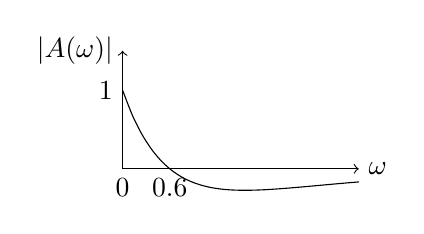
\begin{tikzpicture}
      \draw[->] (0,0) -- (3,0) node[right] {$\omega$};
      \draw[->] (0,0) -- (0,1.5) node[left] {$|A(\omega)|$};
      \draw[domain=0:3,smooth,variable=\x,black] plot ({\x},{2*exp(-sqrt(3)*\x)-exp(-\x/sqrt(3))});
      \draw (0,0) node[below]{0};
      \draw (0.6,0) node[below]{0.6};
\draw (0,1) node[left]{1};
\end{tikzpicture}
\end{center}
\item We estimate $x=0$ to be at $t=0.6$ s.
\end{enumerate}
\end{ans}
\begin{qns}[Waveguide]
A waveguide is formed by clamping a rubber sheet along the lines $y = 0$ and $y = b$. Waves on the unconstrained sheet travel at a speed $v$ that is independent of frequency.
\begin{enumerate}[label=(\roman*)]
\item Show that waves propagating in the waveguide have the form\hfill\textbf{[4]}
$$\psi(x,y)=\text{Re}\bigg[A\sin\bigg(\frac{n\pi y}{b}\bigg)e^{i(\omega t-k_xx)}\bigg]$$
where $n$ is a positive integer. Find the relationship between $\omega$ and $k_x$, and sketch it for $n=1,2,3$.\hfill\textbf{[5]}
\item Derive an expression for the phase velocity, $v_p$, of guided waves.\hfill\textbf{[2]}
\item Calculate $k_x$ and $v_p$ for waves of frequency 200 Hz propagating in the $n = 1$ and $n = 2$ modes for $b = 0.1$ m and $v = 10$ ms$^{-1}$.\hfill\textbf{[3]}
\item A superposition of waves is launched into the waveguide by oscillating the edge of the sheet at $x = 0$ with a profile
$$\psi(0,y)=A(\sin10\pi y+\sin20\pi y)\cos(400\pi t)$$
where here $y$ and $t$ are respectively the values of distance across the waveguide measured in metres and time measured in seconds. Find the first distance, $x_1$, along the waveguide where the profile of the wave is given by \hfill\textbf{[4]}
$$\psi(x_1,y)=A(\sin10\pi y-\sin20\pi y)\cos(400\pi t+\phi)$$
\item Why would propagation in different modes present a problem in optical fibre waveguides for telecommunications systems, and how is this problem avoided in practice?\hfill\textbf{[2]}
\end{enumerate}
\end{qns}
\begin{ans}\leavevmode
\begin{enumerate}[label=(\roman*)]
\item We have two waves of sample amplitude $C$ but with relative phase of $\pi$ radians. Their wavevectors are $(k_x,+k_y)$ and $(k_x,-k_y)$. We have
$$\psi(x,y)=\text{Re}[Ce^{i(\omega t-k_xx-k_yy+\pi)}+Ce^{i(\omega t-k_xx+k_yy)}]=\text{Re}[e^{i(\omega t-k_xx)}2iC\sin(k_yy)]$$
where $A=2iC$. To fulfill the boundary condition $\psi(x,0)=\psi(x,b)=0$, we must have $k_y=\frac{n\pi}{b}$, which gives us the desired relation. The 2D wave equation is $\frac{\partial^2\psi}{\partial t^2}=v^2(\frac{\partial^2\psi}{\partial x^2}+\frac{\partial^2\psi}{\partial y^2})\implies-\omega^2=-v^2(k_x^2+k_y^2)$ and so $\omega=v\sqrt{k_x^2+\frac{n^2\pi^2}{b^2}}$. Plotting the cases $n=1$, 2 and 3, we see that all curves asymptotically approach $\omega=vk_x$ (red line) from above, and intercept the $\omega$-axis at $\frac{nv\pi}{b}$.
\item We have $v_p=\frac{\omega}{k_x}=v\sqrt{1+\frac{n^2\pi^2}{k_x^2b^2}}$ since waves travel in $k_x$-direction.
\item $k_x^2=\frac{\omega^2}{v^2}-\frac{n^2\pi^2}{b^2}$ and hence $k_x(n)=\sqrt{\frac{4\pi^2(200)^2}{10^2}-\frac{\pi^2n^2}{0.1^2}}$. For $n=1$ and $n=2$, we have $k_x=121.7$ m/s and $108.8$ m/s respectively. Also, $v_p(n)=\frac{2\pi f}{k_x(n)}=\frac{2\pi(200)}{k_x(n)}$, we have $10.3$ m/s and 11.5 m/s for $n=1$ and $n=2$ respectively.
\item Given form of $\psi(0,y)$, only the $n=1$ and $n=2$ modes are activated. At $x_1$, the relative phase difference between the two modes is $\pi$, and so $x_1(k_1-k_2)=\pi\implies x_1=\frac{\pi}{k_1-k_2}=\frac{\pi}{121.7-108.8}=0.24$ m.
\item When different modes are present, the signal output at any given time will be superimposed, time-delayed copies of different input signals. This can be mitigated by
\begin{itemize}
    \item choosing physical dimensions such that only one mode propagates;
    \item choosing physical dimensions such that while many many modes are activated, but very little power will be injected into high $n$ modes, and most will go into modes already in the asymptotically linear regime where $\omega\approx v_sk_x$ and so exhibit no dispersion;
    \item undo the dispersion in software later.
\end{itemize}
\end{enumerate}
\end{ans}
\begin{qns}[Fraunhofer Diffraction]
The Fraunhofer diffraction pattern of a two-dimensional aperture defined by $h(x,y)$ illuminated at normal incidence by light of wavevector $k$ is given by
$$\psi(p,q)\propto\int\int h(x,y)e^{-i(px+qy)}dxdy$$
where $q = k sin\theta$ and $p = k sin\xi$, and $\theta$ and $\xi$ are the diffraction angles in the $x$ and $y$ directions respectively.
\begin{enumerate}[label=(\roman*)]
\item Under what conditions is this expression valid?\hfill\textbf{[2]}
\item Derive and explain Babinet’s principle relating to complementary apertures.\hfill\textbf{[5]}
\item Collimated light of wavelength 500 nm is incident normally on a rectangular obstruction of size 0.2mm $\times$ 0.5 mm. The diffracted light is collected with a lens of focal length 20 cm and the diffraction pattern is recorded on a screen placed 20 cm behind the lens. The planes of the obstruction, lens and screen are all parallel. Make a sketch, annotated with quantitative detail, of the intensity on the screen.\hfill\textbf{[6]}
\item Find the diffraction pattern of the more complicated obstruction comprising three rectangles as shown below, and sketch a graph of the intensity distribution on the screen along the direction parallel to $x$.\hfill\textbf{[7]}
\end{enumerate}
\begin{figure}[H]
    \centering
    \includegraphics[scale=0.45]{2016P2B8Q.PNG}
\end{figure}
\end{qns}
\newpage
\begin{ans}\leavevmode
\begin{enumerate}[label=(\roman*)]
\item The expression is valid when the phase variation across the aperture is linear in distance moved across the aperture when viewed from any point of interest on the aperture screen.
\item Babinet's principle states that the intensity of the diffraction pattern of the aperture function $h$ is identical to that of its complementary aperture function $h'(x,y)=1-h(x,y)$, except at the origin.
$$\psi'=A\int h'(x,y)e^{-i(px+qy)}dxdy=A\int(1-h(x,y))e^{-i(px+qy)}dxdy=4\pi^2A\delta(px)\delta(q,y)-\psi(x,y)$$
The first term vanishes off-axis, and so the corresponding intensity is $I'=|\psi'|^2=|0-\psi|^2=|\psi|^2=I$.
\item We have
$$\psi\propto\int_{-a}^a\int_{-b}^be^{-ipx}e^{-iqy}dxdy\propto\bigg[-\frac{1}{ip}e^{-ipx}\bigg]_{-a}^a\bigg[-\frac{1}{iq}e^{-iqy}\bigg]_{-b}^b\propto\sinc(pa)\sinc(qb)$$
The zeroes of the intensity pattern occur when $pa=n\pi$, $qb=m\pi$ for $m,n\in\mathbb{Z}^+$, i.e. at angles $\theta=\sin^{-1}(m\pi/bk)=\sin^{-1}(m\lambda/2b)$ and $\xi=\sin^{-1}(n\pi/ak)=\sin^{-1}(n\lambda/2a)$ which correspond to positions $(X,Y)$ in the focal plane where $Y=f\tan\xi$, $X=f\tan\theta$, with $f$ being the focal length. We have $\frac{\lambda}{2a}=\frac{500\times10^{-9}}{2(0.5\times10^{-3}}=5\times10^{-4}<<1$, so $\tan(\sin^{-1}(\phi))\approx\phi$ $\forall\phi$. So zeroes occur at $Y=f\frac{n\lambda}{2a}=n(1\times10^{-4})$ m and $X=f\frac{m\lambda}{2b}=m(2.5\times10^{-4})$ m.
\begin{figure}[H]
    \centering
    \includegraphics[scale=0.7]{2016P2B8i.PNG}
    \caption{Amplitude monochrome plot of $\sinc(5p)\sinc(2q)$ in $(p,q)$ plane. Positions of minima on the screen are at $(X,Y)=(m2.5\times10^{-4}, n1\times10^{-4})$.}
\end{figure}
\item We convolve the old aperture function with
$$g=\delta(x+c)+\delta(x)+\delta(x-c)$$
with $c=1.0$ mm. By the convolution theorem, the amplitude acquires a further fact of $\tilde{g}$
$$\tilde{g}=1+2\cos\frac{2\pi X}{f\lambda}c$$
The previous pattern has extra fringes now, given by the zeroes of $\tilde{g}$ where $\frac{2\pi Xc}{f\lambda}=2\frac{\pi}{3}N$ where $N$ is an integer not zero modulo 3. There are extra zeroes with a spacing of $\Delta x=\frac{f\lambda}{2c}=1.66\times10^{-5}$, but missing out every third one.
\begin{figure}[H]
    \centering
    \includegraphics[scale=0.5]{2016P2B8ii.PNG}
    \caption{Plot of intensity pattern with (blue) and without (orange) $\tilde{g}$.}
\end{figure}
\end{enumerate}
\end{ans}
\newpage
\begin{qns}[Fabry-Pérot]\leavevmode
\begin{enumerate}[label=(\roman*)]
\item A Fabry–Pérot etalon comprises two semi-transparent mirrors separated by an air gap of thickness $d$. Each mirror has (intensity) reflection and transmission coefficients $R$ and $T$ respectively. Consider the simple case where the etalon is illuminated with collimated light of wavelength $\lambda$ at normal incidence, and the transmission of the etalon is measured in the same direction. Show that the transmission of the etalon is given by
$$B=\frac{T^2}{1+R^2-2R\cos\delta}$$
where $\delta=\frac{4\pi d}{\lambda}$.\hfill\textbf{[5]}
\item Show that for highly reflective mirrors the half-width at half maximum of each peak is given by\hfill\textbf{[3]}
$$\delta_{1/2}\approx\frac{1-R}{\sqrt{R}}$$
\begin{mdframed}
\textcolor{darkblue}{You may find it convenient to note, and may assume without proof, that the expression above for $B$ can be rearranged as
$$B=\frac{T^2}{(1-R)^2}\frac{1}{1+[4R/(1-R)^2]\sin^2(\delta/2)}$$}
\end{mdframed}
\item  Calculate $\delta_{1/2}$ for $R = 0.80$ and sketch $B$ as a function of $\delta$ for an etalon with $R = 0.80$ and $T = 0.20$.\hfill\textbf{[3]}
\item The etalon described above is illuminated with light containing wavelengths of 1000.0 nm and 1000.2 nm with equal intensity. Sketch the output intensity of the etalon as a function of d as $d$ is increased from 0.4998 mm to 0.5003 mm. Indicate the values of $d$ at which any peaks occur, and comment on whether it is possible to resolve the two wavelength components in the spectrum.\hfill\textbf{[6]}
\item A third wavelength component at 1001.1 nm is added to the input spectrum. Add any new peaks that arise in your sketch above, and comment on the implications for spectroscopy using a Fabry-Pérot etalon.\hfill\textbf{[3]}
\end{enumerate}
\end{qns}
\begin{ans}\leavevmode
\begin{enumerate}[label=(\roman*)]
\item Let the amplitude reflection and transmission coefficients for a single mirror be $r$ and $t$ respectively. For a beam of initial amplitude $A$ to be transmitted through the entire system it needs to have been transmitted through both mirrors once each and reflected from each mirror the same number of times. The optical path difference between two consecutive outgoing wave is $2d\sec\theta-2d\tan\theta\sin\theta=2d\cos\theta$. Each round trip of two reflections also picks up a phase $\delta=k2d\cos\theta=\frac{4\pi d}{\lambda}\cos\theta$,
\begin{figure}[H]
    \centering
    \includegraphics[scale=0.75]{2016P2B9ii.PNG}
\end{figure}
and so the amplitude of a transmitted beam that has gone through $n$ round trips in the air-gap is $\psi=At^2e^{in\delta}r^{2n}$. The total amplitude is given by
$$\psi_{tot}=\sum_{n=0}^\infty At^2e^{in\phi}r^{2n}=At^2\frac{1}{1-r^2e^{i\phi}}$$
The net transmission coefficient is
$$B:=\frac{|\psi_{tot}|^2}{|A|^2}=\frac{t^4}{(1-r^2e^{i\delta})(1-r^2e^{-i\delta})}=\frac{t^4}{1-r^2(e^{-i\delta}+e^{i\delta})+r^4}=\frac{T^2}{1+R^2-2R\cos\delta}$$
where $R=|r|^2$ and $T=|t|^2$.
\item We are given that $B$ is equal to the expression
$$B=\frac{T^2}{(1-R)^2}\frac{1}{1+\frac{4R}{(1-R)^2}\sin^2(\delta/2)}$$
$B_{max}$ occur when $\cos\delta=1$ so $B_{max}=\frac{T^2}{(1-R)^2}$ and hence half-power points occur when $B=\frac{1}{2}B_{max}$ and this means $\sin(\delta_{1/2}/2)=\frac{1-R}{2\sqrt{R}}$. Assume $\sin(\delta_{1/2}/2)\approx\delta_{1/2}/2$, then we have
$$\delta_{1/2}\approx\frac{1-R}{\sqrt{R}}$$
\item We have $R=0.80$ and so $\delta_{1/2}\approx\frac{1-0.80}{\sqrt{0.80}}=0.224$. We thus have $B=\frac{0.2^2}{0.2^2}\frac{1}{1+4(0.80)/0.2^2}\sin^2(\delta/2)=\frac{1}{1+80\sin^2(\delta/2)}$.
\begin{center}
\begin{tikzpicture}
      \draw[->] (0,0) -- (8,0) node[right] {$\delta$};
      \draw[->] (0,0) -- (0,2.5) node[left] {$B(\delta)$};
      \draw[domain=0:8,smooth,variable=\x,blue] plot ({\x},{1/(1+80*(sin(\x*180/(2*pi)))^2)});
      \draw (0,0) node[below]{0};
    \draw (0,1) node[left]{1};
    \draw (0,0.5) node[left]{0.5};
\end{tikzpicture}
\end{center}
\item Assume normal incidence, then we have $m=\frac{2d}{\lambda}$. For $\lambda=1000$ nm, $d\in[0.4998mm, 0.5003mm]$, and hence $m\in[999.6,1000.6]$, hence $m=1000$ at $d=0.5$ mm. For $\lambda=1000.2$ nm, $d\in[0.4998mm,0.5003mm]$, and so $m\in[999.4,1000.4]$, and hence $m=1000$ at $d=0.501$ mm. Their widths at half-maximum was found to be 0.224, which is much less than the separation between peaks. By Rayleigh's criterion, the peak can be resolved.
\item By a similar computation, the peak of $\lambda=1001.1$ nm is at $d=0.50005$ mm, which is midway between the previous two. By Rayleigh's criterion, the full width half maximum is still less than the separation between the peaks, hence still resolvable.
\end{enumerate}
\end{ans}
\newpage
\subsubsection{Section C}
\begin{qns}[Transport]\leavevmode
\begin{enumerate}[label=(\roman*)]
\item Briefly explain, with the aid of a diagram, the origin of the transverse voltage which arises when a magnetic field is applied perpendicularly to a current flow in a conducting bar (the Hall effect). State one property of a periodic solid that may be determined from a measurement of the Hall effect.\hfill\textbf{[5]}
\item The semi-classical equation governing the transport of electrons in a periodic lattice under the application of an electric field $\mathbf{E}$ and magnetic field $\mathbf{B}$ is
\begin{equation}
  m^*\frac{d\langle\mathbf{v}\rangle}{dt}=-\frac{m^*}{\tau}\langle\mathbf{v}\rangle+e\mathbf{E}+e\langle\mathbf{v}\rangle\times\mathbf{B}\tag{*}  
\end{equation}
where $e$ is the electron charge, $m^*$ their effective mass, and $\tau$ is the mean time between collision of electrons with lattice defects or phonons. Explain the origin of each term in this equation.\hfill\textbf{[2]}
\begin{figure}[H]
    \centering
    \includegraphics[scale=0.5]{2016P2C10Q.PNG}
\end{figure}
\item A Hall bar has length $l$, width $w$, and thickness $t$, and is oriented as shown in the diagram. A current $I = (I_x, 0, 0)$ flows through the bar and $\mathbf{B}=(0,0,B_z)$. Using equation (*) above, derive expressions for the steady state electric field components within the bar, $\mathbf{E}=(E_x,E_y,E_z)$.\hfill\textbf{[3]}
\item Determine expressions for the conductivity, $\sigma$, and Hall coefficient, $R_H=\frac{E_y}{j_xB_z}$, where $j_x$ is the current density in the bar.\hfill\textbf{[2]}
\item The measured potential difference across the length of the bar is $V_x$, and across the width is $V_y$. Show that\hfill\textbf{[1]} 
$$\frac{V_y}{V_x}=-\frac{eB_z}{m^*}\tau\frac{w}{l}$$
\item A Hall bar made from high-purity Cu, with $t = 5$ $\mu$m and $l/w = 10$, has a measured resistance of $R = 11m\Omega$ across its length. Determine the free electron density in Cu, given that $V_y/V_x=0.013$ when $B_z = 10$ T.\hfill\textbf{[3]}
\item Assuming $m^*=m_e$ for Cu, estimate the mean electron scattering time $\tau$. Justify why this a good assumption in the case of Cu, which may be considered as a monovalent metal.\hfill\textbf{[4]}
\end{enumerate}
\end{qns}
\newpage
\begin{ans}\leavevmode
\begin{enumerate}[label=(\roman*)]
\item If a steady current flows in a conductor under the influence of a magnetic field $B$, then there will be a transverse Lorentz force $q\mathbf{v}\times\mathbf{B}$ acting on the charge carriers of charge $q$ travelling with velocity $\mathbf{v}$. As the deflected charge carriers accumulate on one side of the conductor, a static charge density gradient is resulted, in turn leading to an opposing electric field to cancel the Lorentz force. This continues until an equilibrium is achieved and the charge carriers proceed undeviated. This is independent of the current direction. This Hall effect allow us to measure the Hall coefficient, which gives us the number density of the charge carriers. 
\item The effective mass $m^*$ is the resistance to acceleration of the charge carrier. In a strongly interacting system, the electron's effective mass will not be equal to its mass in the absence of the periodic lattice. The last two force terms are from the Lorentz force law. The first term on the RHS is the rate of loss of momentum due to collisions with the lattice.
\item The current is the cross-sectional area multiplied by the current density
$$I_x=twJ_x=twnv_xq$$
for electrons, both $v,q<0$, so $I_x$ is independent of charge carrier's sign. For steady state, LHS of (*) is zero, so $\mathbf{B}\perp\langle\mathbf{v}\rangle$, so 
$$E_y=-\frac{I_xB_z}{twne}=-v_xB_z$$
No acceleration in $z$-direction, so $E_z=0$, but there is current flowing in the resistive material in the $x$-direction, so from Ohn's Law
$$E_x=\frac{I_x}{\sigma tw}$$
\item Since acceleration is zero and the magnetic term is zero, (*) gives
$$\frac{m^*I_x}{\tau ntwe}=\frac{eI_x}{\sigma tw}\implies\sigma=\frac{e^2n\tau}{m^*}$$
The Hall coefficient will be
$$R_H=\frac{E_y}{j_xB_z}=\frac{-v_xB_z}{nv_xqB_z}=\frac{-1}{ne}$$
\item The ratio of potential differences is
$$\frac{V_y}{V_x}=\frac{E_yw}{E_xl}=\frac{w}{l}\frac{J_xB_z}{ne}\frac{\sigma}{J_x}=\frac{wB_ze^2n\tau}{lnem^*}=\frac{eBz\tau w}{m^*l}$$
\item We have two expressions for conductivity, either via definition $\sigma=\frac{l/w}{Rt}$ or from part (iv), $\sigma=\frac{ne^2\tau}{m^*}$. Then, we have for number density
$$n=\frac{l/w}{Rt}\frac{m^*}{e^2\tau}=\frac{l/w}{Rt}\frac{1}{e^2}\frac{V_x}{V_y}\frac{eB_zw}{l}=\frac{10}{11\times10^{-3}(5\times10^{-6})}\frac{1/0.013}{9.11\times10^{-31}}=8.7\times10^{28}m^{-3}$$
where we used result in part (v).
\item We assume $m=m^*$ since for monovalent metals, the Fermi surface is well within the first Brillouin Zone, and so the lattice distortions are not going to significantly affect the dispersion relation.
$$\tau=\frac{V_y}{V_x}\frac{l}{w}\frac{m}{eB_z}=\frac{0.013\times 10\times 9.11\times10^{-31}}{10\times 1.6\times10^{-19}}=7.40\times10^{-14}s$$

\end{enumerate}
\end{ans}
\newpage
\begin{qns}[Structure]\leavevmode
\begin{enumerate}[label=(\roman*)]
\item What is meant by the term reciprocal lattice?\hfill\textbf{[2]}\\[5pt]
A plane wave of wavevector $\mathbf{k_i}$ is incident on a crystal having identical atoms at points $\mathbf{r_n}$ relative to the origin, O. Diffraction from the periodic structure produces an outgoing plane wave of wavevector $\mathbf{k_f}$, which is measured at detector, D, at a distance from the crystal $>>|\mathbf{r_n}|$.
\item Consider the scattering of the incident plane wave from two atoms, one at O and one at $\mathbf{r_n}$. Sketch this geometry, including the vectors $\mathbf{k_i}$, $\mathbf{k_f}$, $\mathbf{r_n}$.\hfill\textbf{[2]}
\item Show that the phase difference between the scattered waves arriving at D from these two atoms is given by $\mathbf{k_s}\cdot\mathbf{r_n}$, where $\mathbf{k_s}=\mathbf{k_i}-\mathbf{k_f}$ and hence that the total amplitude, $S$ , of the outgoing wave measured at D may be written as $S$ directly proportional to\hfill\textbf{[5]}
$$\sum_ne^{i\mathbf{k_s}\cdot\mathbf{r_n}}$$
\item Let $\mathbf{a}$, $\mathbf{b}$, $\mathbf{c}$ be the primitive unit cell vectors of the crystal lattice. A general reciprocal lattice vector takes the form:
$$\mathbf{G_{hkl}}=h\mathbf{A}+k\mathbf{B}+l\mathbf{C}$$
where $h$, $k$ and $l$ are integers. Write down values for $\mathbf{A}\cdot\mathbf{a}$, $\mathbf{A}\cdot\mathbf{b}$ and $\mathbf{A}\cdot\mathbf{c}$ and show that diffraction maxima will be observed at D when $\mathbf{k_s}$ is equal to a reciprocal lattice vector.\hfill\textbf{[4]}
\item A two-dimensional crystal contains one type of atom. The atomic spacing is $a$ along each axis of the primitive unit cell, and the angle between the axes is $\pi/3$ rad. Find the general reciprocal lattice vector $\mathbf{G_{hk}}$ for this crystal and draw labelled sketches of both the primitive unit cell and reciprocal lattice. Calculate the smallest value of $|\mathbf{k_s}|$ for which a diffraction maximum will be measured at D. (You may ignore contributions from lattice vibrations.)\hfill\textbf{[7]}
\end{enumerate}
\end{qns}
\begin{ans}\leavevmode
\begin{enumerate}[label=(\roman*)]
\item A reciprocal lattice is the dual (via a Fourier transform) of a given lattice, such that in any dot product of two vectors in a space, it is convenient to represent one of them in the lattice basis, and the other in reciprocal lattice basis such that the cross terms cancel.
\item Incident plane wave and scattered plane wave have wavevectors $\mathbf{k_i}$ and $\mathbf{k_f}$ respectively. The angle subtended from the vertical $\theta$ by either plane wave is the same.
\item The phase difference is $$\Delta\phi=|\mathbf{k_i}|AB-|\mathbf{k_f}|OC=\mathbf{r_n}\cdot(\mathbf{k_i}-\mathbf{k_f})=\mathbf{r_n}\cdot\mathbf{k_s}$$
Sum over all scattering centres to get $S\propto \sum_ne^{i\mathbf{k_n}\cdot\mathbf{r_n}}$.
\item We follow the crystallographic convention: $\mathbf{A}\cdot\mathbf{a}=2\pi,~\mathbf{A}\cdot\mathbf{b}=0,~\mathbf{A}\cdot\mathbf{c}=0$. The scattering centres scatter in phase when $\mathbf{r_n}\cdot\mathbf{k_s}$ is an integer number times $2\pi$ for every term in the sum
$$\mathbf{r_n}\cdot\mathbf{k_s}=(\lambda\mathbf{a}+\mu\mathbf{b}+\nu\mathbf{c})\cdot(h\mathbf{A}+k\mathbf{B}+\ell\mathbf{C})=2\pi(h\lambda+k\mu+\ell\nu)$$
and this is required to be an integer number of $2\pi$, hence $\ell,h,k$ are separately integers.
\item The angle between the axes is $\frac{\pi}{3}$. Without loss of generality, let the real space vectors be $\mathbf{a}=a(1,0)^T$ and $\mathbf{b}=a(\cos(\pi/3),\sin(\pi/3))^T=a(1/2,\sqrt{3}/2)^T$. Then the reciprocal lattice vectors will be 
$$\mathbf{A}=\frac{2\pi}{a}\frac{2}{\sqrt{3}}\begin{pmatrix}\sqrt{3}/2\\-1/2\\\end{pmatrix},\quad \mathbf{B}=\frac{2\pi}{a}\frac{2}{\sqrt{3}}\begin{pmatrix}0\\1\\\end{pmatrix}$$
Hence, the general reciprocal lattice vector is
$$\mathbf{G_{hk}}=\frac{4\pi}{a\sqrt{3}}\bigg[h\begin{pmatrix}\sqrt{3}/2\\-1/2\\\end{pmatrix}+k\begin{pmatrix}0\\1\\\end{pmatrix}\bigg]$$
For minimum $|\mathbf{k_s}|$, either $h$ or $k$ is equal to 1 while the other value is zero. Hence, $|\mathbf{k_s}|=4\pi/\sqrt{3}$.
\end{enumerate}
\end{ans}
\newpage
\subsubsection{Section D}
\begin{qns}[OWO Essay]
Write an essay on Fresnel diffraction, including detailed discussion of the Fresnel diffraction patterns of edges and rectangular apertures.\hfill\textbf{[20]}
\end{qns}
\begin{ans}
Consider a spherical source with strength $a_S$, at distance $s(x,y)$ from the aperture element $dxdy$ (with overall aperture function $h(x,y)$, then the total amplitude at point P, at a distance $r$ from the aperture element, is
$$\psi_P=-\int\frac{i}{\lambda}h(x,y)K(\theta)\frac{a_Se^{ik(s+r)}}{sr}dxdy$$
where $K(\theta)$ is the obliquity factor. This is the Fresnel-Kirchhoff diffraction integral, which is valid in the limit of distances greater than the wavelength of light, allowing us to neglect the vector nature of the electromagnetic wave. In the case of Fresnel diffraction (diffracted beam on-axis), we assume further that
\begin{itemize}
    \item the angles to the edge of the aperture are small enough that we can neglect the obliquity factor, and thus take $K(\theta)=1$;
    \item that the variations in $r_1$ and $r_2$ over the aperture are negligible as far as the denominator is concerned: $r_1\sim a$ and $r_2\sim b$ but note variations in $(r_1+r_2-a-b)$ are not negligible compared with $\lambda$ and so have a significant effect on the phase term.
\end{itemize}
Under these approximations, we have $\psi_P(0,0)$ to be directly proportional to
$$\int_\Sigma h(x,y)e^{ik(x^2+y^2)/2R}dxdy$$
where the path from S to P via the aperture element at $(x,y)$ is
$$r_1+r_2\approx a+b+\frac{x^2+y^2}{2a}+\frac{x^2+y^2}{2b}$$
Writing $\frac{1}{R}=\frac{1}{a}+\frac{1}{b}$, we have the optical path to be directly proportional to $(x^2+y^2)/2R$. Here, the quadratic phase in the diffraction integral can't be ignored since the distances between the screen and the aperture is of order $D^2/\lambda$ or smaller, where $D$ is the maximum dimension of the aperture.\\[5pt]
Consider a uniform rectangular aperture in the Fresnel diffraction limit. Since the aperture function is separable, the diffraction integral is
$$\int_{x_1}^{x_2}e^{ikx^2/2R}dx\int_{y_1}^{y_2}e^{iky^2/2R}dy=\int_{u_1}^{u_2}e^{i0.5\pi u^2}du\int_{v_1}^{v_2}e^{i0.5\pi v^2}dv$$
where $u=x\sqrt{2/(\lambda R)}$ and $v=y\sqrt{2/(\lambda R)}$. The Fresnel integrals will be $C(w):=\int_0^w\cos(\pi u^2/2)du$ and $S(w):=\int_0^w\sin(\pi u^2/2)du$. When we plot $C(w)+iS(w)$ on the complex plane, the locus of these points is known as the Cornu spiral, shown below:
\begin{figure}[H]
    \centering
    \includegraphics[scale=0.5]{2010P1B9Q.PNG}
\end{figure}
The parameter $w$ is the arc length parameter along the curve. The arc length $l$ along the curve between two points $w_1$ and $w_2$ is equal to $w_2-w_1$.
$$dl^2=dC^2+dS^2=dw^2[\cos^2(0.5\pi w^2)+\sin^2(0.5\pi w^2)]=dw^2\implies dl=dw$$
The radius of curvature $R_C$ at a point $w$ is
$$\frac{1}{R_C}=\frac{C'S''-S'C''}{(C'+S')^{1.5}}=\pi w$$
Other features of the Cornu Spiral:
\begin{itemize}
    \item The curve spirals in towards the point $(C(\infty), S(\infty))=(0.5,0.5)$. 
    \item The curve has odd symmetry since $C$ and $S$ are odd functions.
    \item The curve has a local  vertical gradient when $w=\sqrt{2m+1}$, $m\in\mathbb{Z}^+\cup\{0\}$ and $w=\sqrt{2m}$.
    \item The slope of the tangent vector is $\frac{S'(w)}{C'(w)}=\tan(0.5\pi w^2)$.
\end{itemize}
Consider the wavefront obstructed by a straight edge. Define the origin O$_b$ in the aperture plane to be at the edge of the obstruction. Fresnel conditions are satisfied since S, O$_b$ and b are in a straight line. The diffracted wave at $b$ is $\psi_p(b)=[C(\infty)-C(0)]+i[S(\infty)-S(0)]=(0.5,0.5)$, where we only considered the half of the Cornu spiral in the first quadrant. This is half the amplitude (and hence one quarter the intensity) if there was no obstruction, which is the entire Cornu spiral. To calculate the diffracted wave at other points on the screen, we move the origin so that it is still between S and our observation point, and Fresnel conditions are still satisfied.
\begin{figure}[H]
    \centering
    \includegraphics[width=\linewidth]{fresneledge.PNG}
    \caption{(Left) Geometry of problem; (Centre) Cornu Spiral with diffraction amplitude at the four points labelled; (Right) Variation of intensity for diffraction pattern.}
\end{figure}
Well outside the shadow, the intensity is the same as for an unobstructed wavefront. The intensity at the geometric edge is 25 percent of the unobstructed intensity $I_u$. The intensity falls smoothly inside the geometric shadow, roughly as $1/w^2$. There are fringes outside the geometric shadow, producing a maximum intensity 138 percent of $I_u$ at point d, just outside the edge. This is due to the wave nature of light.\\[5pt]
To explain the origin of this pattern, we consider the point O at the straight edge and the point P directly ahead of O. The line OP defines the geometric shadow. Below O, the screen cuts off the wavefront. The phase difference between the contributions to the disturbance at P from O and from a point H, height $h$ above O is
$$\Delta(h)=\frac{2\pi}{\lambda}(HP-OP)=\frac{2\pi}{\lambda}(\sqrt{h^2+l^2}-l)\approx\frac{2\pi}{\lambda}l\bigg(1+\frac{h^2}{2l^2}\bigg)-l=\frac{\pi h^2}{\lambda l}$$
Divide the wavefront above O into strips parallel to the infinite straight edge. Choose the width of these strips such that successive strips differ in phase by $\pi$ radians, in their contributions to the disturbance at P. We obtain the Fresnel integrals with $w:=h\sqrt{2/\lambda l}$.
\end{ans}
\newpage
\begin{qns}
Write brief notes on two of the following:\hfill\textbf{[20]}
\begin{itemize}
    \item successes and failures of the free electron model;
    \item the thermal conductivity of an insulator, including a discussion of its temperature dependence; 
    \item  the use of p-n junctions in semiconductor devices.
\end{itemize}
\end{qns}
\begin{ans}\leavevmode
\subsubsection*{Successes and failures of the free electron model:}
In the free electron model (FEM), each lattice point contributes $n$ delocalized electrons ($n$ is valency). The rest are regarded as core electrons and together with the nuclei, they form a uniform background potential. This is known as the Drude-Sommerfeld model. We will first look at the classical Drude model. The assumptions of Drude model are
\begin{enumerate}
    \item Independent electron approximation: neglect electron-electron interactions between collisions; Free electron approximation: neglect electron-ion interactions. The electrons respond solely to the externally applied fields.
    \item Collisions are instantaneous events that abruptly alter the velocity of an electron. Drude attributed them to the electrons bouncing off the impenetrable ion cores.
    \item Electron experiences a collision with a probability per unit time $1/\tau$, where $\tau$ is the relaxation time. An electron picked at random at a given moment will, on the average, have been travelling for a time $\tau$ before its next collision, and will, on the average, have been travelling for a time $\tau$ since its last collision. $\tau$ is independent of the electron's position and velocity.
    \item Electrons are assumed to achieve thermal equilibrium with their surroundings only through collisions. Immediately after each collision, an electron is taken to emerge with a velocity that is not related to its velocity just before the collision, but randomly oriented and with a speed appropriate to the temperature prevailing at the place where the collision occurred.
\end{enumerate}
Drude theory is successful in accounting for the value of Wiedemann-Franz ratio. The Weidemann-Franz law states that the ratio of thermal conductivity $\kappa$ to electrical conductivity $\sigma$ is directly proportional to the temperature. The Lorenz number is
$$\frac{\kappa}{\sigma T}=\frac{3k_B^2}{2e^2}$$
Many other transport properties are predicted correctly, e.g. AC electrical conductivity at finite frequency. 
$$\sigma_{AC}(\omega)=\frac{1}{1+i\omega\tau}\frac{ne^2\tau}{m}=\frac{ne^2\tau}{m}\frac{1-i\omega\tau}{1+\omega^2\tau^2}$$
The Hall coefficient $R_H=-\frac{1}{ne}$ measurement of the number density of charge carriers seems reasonable for many metals. But yet, the Hall coefficient is frequently measured to have the wrong sign, indicating a charge carrier with charge opposite to that of the electron. Furthermore, there is no $\frac{3}{2}k_B$ heat capacity per particle measured for electrons in metals, but rather the experimental relation is $\gamma T+\epsilon T^3$. This can be partially resolved if we further consider the quantum statistics of electrons, i.e. Fermi-Dirac statistics. The Fermi-Dirac distribution is
$$n_{FD}=\frac{1}{e^{(\epsilon-\mu)/k_BT}+1}$$
Under Born-von Karman boundary conditions (or sometimes called periodic boundary conditions), the solution is $\psi_k(\mathbf{r})=\frac{1}{\sqrt{V}}e^{i\mathbf{k}\cdot\mathbf{r}}$ with energy $\epsilon(\mathbf{k})=\frac{\hbar^2k^2}{2m}$. The periodic boundary condition require quantization of wavevectors $k_i=\frac{2\pi n_i}{L}$, $n_i\in\mathbb{Z}$. If the region is very large, then to an excellent approximation, the number of allowed points is just the volume of $k$-space contained within the region, divided by the volume of $k$-space per point in the network of allowed values of $\mathbf{k}$. We conclude that a region of $k$-space of volume $\Omega$ will contain $\frac{\Omega V}{8\pi^3}$ allowed values of $\mathbf{k}$.\\[5pt]
Assuming the electrons are non-interacting, we can build up the $N$-electron ground state by placing electrons into the allowed one-electron levels. The Pauli exclusion principle states that we at most place on electron in each single electron level. But, associated with each allowed wavevector $\mathbf{k}$ are two electronic levels.\\[5pt]
We begin placing the electrons from the lowest energy and then successively filling the one-electron levels of lowest energy that are not occupied. Since the energy of a one-electron level is directly proportional to the square of its wave vector, when $N$ is enormous, the occupied region will be indistinguishable from a sphere. The radius of this sphere is called $k_F$ and its volume $\Omega$ is $\frac{4}{3}\pi k_F^3$. The corresponding highest energy occupied state is the Fermi energy $E_F$. The number of allowed values of $\mathbf{k}$ within the sphere is $\frac{4\pi k_F^3}{3}\frac{V}{8\pi^3}=\frac{k_F^3V}{6\pi^2}$. The number of electrons will be twice of this and so the electronic density is $n=\frac{k_F^3}{3\pi^2}$. The density of states can be worked out to be
$$g(E)=\frac{V}{2\pi^2}(2m/\hbar^2)^{1.5}E^{0.5}$$
Only the electrons within $k_BT$ of the Fermi energy $E_F$ can be thermally activated, since the electrons deep in the Fermi sphere have no available states to excite to. There are a total of $g(E_F)k_BT$ number of these. Assume each electron has $\frac{3}{2}k_BT$ thermal energy, then the total electronic energy is
$$U_{el}=\frac{3}{2}k_BTg(E_F)k_BT$$
Since $N=\frac{V}{2\pi^2}(2m/\hbar^2)^{3/2}\int_0^{E_F}E^{1/2}dE$, $g(E_F)=\frac{V}{2\pi^2}(2m/\hbar^2)^{3/2}E_F^{1/2}=\frac{3N}{2E_F}$, and hence 
$$C_{el}=\frac{\partial U_{el}}{\partial T}\approx\frac{3N}{2k_BT_F}3k_B^2T=\frac{9Nk_BT}{2T_F}$$
One example where this approximation is in good agreement with experiment, is Sodium. The free electron model can account for the linear temperature dependence, but in general, both electrons and phonons contribute to heat capacity. We note that the phononic contributions completely dominate the specific heat at high temperatures. Well below the room temperature, their contribution falls off as $T^3$ (Debye's theory), and at very low temperatures it drops below the electronic contribution, which only decreases linearly with $T$ (electronic contribution dominates now), i.e. 
$$C_V=\gamma T+AT^3$$
where $\gamma\approx 1.67$ (in theory) and $A$ are constants. There may be some discrepancy between theory and experiment due to the fact that electrons have an effective mass dependent on the influence of the periodic lattice (not accounted for in the free electron model). Finally, a non-exhaustive limitations of the free electron model is as follow:
\begin{itemize}
    \item The scattering length $\sim v_F\tau$ is about 100 Angstroms, but yet electrons do not scatter in metals. Why?
    \item Why do core electrons not count in the Fermi energy computation? What about insulators, which has no free electrons?
    \item Hall coefficient is still the wrong sign for some materials.
    \item Fail to account for the optical spectra (absorption intensity dependence on frequencies, as well as, colour).
    \item Measured specific heats are still off by factors as large as 10 for some metals.
    \item Electron-electron Coulomb interactions are roughly the same scale as the Fermi energy (Landau Fermi Liquid Theory)
\end{itemize}

\newpage
\subsubsection*{The thermal conductivity of an insulator, including a discussion of its temperature dependence:}
In an insulator, thermal conductivity is largely due to phonons. A phonon is a collective harmonic excitation of the atoms with a well-defined frequency, with a fixed relative phase and amplitude between all of the atoms. Heat is carried by these phonons (and free electrons in conductors). At low temperatures, the thermal conductivity is $\propto T^3$ due to Debye's theory for phononic heat capacity while at high temperatures, the thermal conductivity is $\propto 1/T$ due to the significantly greater occurrence of phonon-phonon scattering.\\[5pt]
Phonons interact through lattice anharmonicity: one phonon $\mathbf{q_2}$ distorts the lattice while another incoming phonon $\mathbf{q_1}$ diffracts off that phonon $\mathbf{q_2}$. Their interactions satisfy $\mathbf{q_3}=\mathbf{q_1}+\mathbf{q_2}$. Phonons can coalesce, i.e. $\hbar\mathbf{q_3}=\hbar\mathbf{q_1}+\hbar\mathbf{q_2}$ (conservation of momentum) and energy is conserved. Similarly, phonons can decompose, i.e. i.e. $\hbar\mathbf{q_3}=\hbar\mathbf{q_1}+\hbar\mathbf{q_2}$ (conservation of momentum) and energy is also conserved. This is the more common phonon-phonon scattering.\\[5pt]
In general, scattering processes reduce the mean free path. The resultant mean free path is a linear sum of the inverse of the mean free path for each contributory process. There are two types of scattering:
\begin{itemize}
    \item Geometric scattering: phonons scatter from sample boundaries and from impurities or grain boundaries. The geometric mean free path $l$ is independent of temperature $T$.
    \item Phonon-phonon scattering: phonons scatter one another in an anharmonic lattice (true crystals are not purely harmonic). 
\end{itemize}
For phonon-phonon scattering, there are two sub-types:
\begin{itemize}
\item Normal scattering: Most phonon coalescence processes don't dramatically change the resulting wavevector, hence weakly affects $\kappa$.
\item Umklapp scattering: These coalescences (which require high temperatures) can result in a phonon wavevector outside the first Brillouin Zone. Folding these back into the first Brillouin Zone results in a negative group velocity. This gives strong randomisation of phonons, hence a dramatic reduction in $\kappa$.
\end{itemize}
Using kinetic theory: we consider phonons crossing a plane at an angle $\theta$, the excess temperature of phonons crossing the plane $\Delta T=-\frac{dT}{dz}l\cos\theta$ and excess energy in each phonon mode $c_{ph}\Delta T=-c_{ph}\frac{dT}{dz}l\cos\theta$, where $c_{ph}$ is the heat capacity of a phonon mode. We integrate the excess heat per mode over the phonon distribution $nf(c)dc$, i.e. the number of phonons with speed $c$ to $c+dc$. The phonons are propagating in all directions, so weight by speed normal to the plane. The fraction with angles $\theta$ to $\theta+d\theta$ is $\frac{2\pi}{4\pi}\sin\theta d\theta$. The heat flux integral across the plane becomes
$$\int_0^\pi\int_0^\infty nf(c)dc\frac{1}{2}\sin\theta d\theta c\cos\theta\bigg(-c_{ph}\frac{dT}{dz}l\cos\theta\bigg)=-\frac{1}{2}c_{ph}nl\frac{dT}{dz}\int_0^\pi\sin\theta\cos^2\theta d\theta\langle c\rangle$$
Since this heat flux is $-\kappa\frac{dT}{dz}$, we obtain the phononic contribution to thermal conductivity be
$$\kappa=\frac{1}{3}C\langle c\rangle l$$
Since phonons are bosons, they follow the Bose-Einstein statistics with probability distribution
$$p_{BE}(\varepsilon)=\frac{1}{e^{\beta(\varepsilon-\mu)}-1}$$
where $\beta=\frac{1}{k_BT}$. At low temperatures, there are few phonons so the thermal conductivity is dominated by the heat capacity with dependence $C\propto T^3$. This follows from Debye's model.\\[5pt]
In Debye's model, we assume the lattice vibrations are waves with speed $v_s$, speed of sound in the solid, i.e. for all wavelengths, we have a linear dispersion relation $\omega=v_sq$, where $q$ is the wavevector of the lattice vibration. The density of states of lattice vibrations in 3D as a function of $q$ is
$$g(q)dq=\frac{4\pi q^2dq}{(2\pi/L)^3}3\implies g(\omega)d\omega=\frac{3V\omega^2d\omega}{2\pi^2v_s^3}$$
such that $\int_0^{\omega_D}g(\omega)d\omega=3N$ where $\omega_D$ the cutoff frequency (Debye frequency) is imposed to have a finite number of modes. We then have $\omega_D^3V=6N\pi^2v_s^3$ and hence rewriting $g(\omega)d\omega=\frac{9N\omega^2d\omega}{\omega_D^3}$. We can thus define a Debye temperature $\Theta_D=\hbar\omega_D/k$. The internal energy is 
$$U=\int_0^{\omega_D}g(\omega)\hbar\omega(0.5+(e^{\beta\hbar\omega}-1)^{-1})d\omega=\frac{9}{8}N\hbar\omega_D+\frac{9N\hbar}{\omega_D^3}\int_0^{\omega_D}\frac{\omega^3d\omega}{e^{\hbar\omega\beta}-1}$$
The heat capacity per mole will be
$$C=\frac{9R}{x_D^3}\int_0^{x_D}\frac{x^4e^xdx}{(e^x-1)^2},\quad x_D=\hbar\beta\omega_D$$
At high temperature
$$C\rightarrow\frac{9R}{x_D^3}\int_0^{x_D}\frac{x^4}{x^2}dx=3R$$ 
as expected. At low temperatures,
$$C\rightarrow\frac{9R}{x_D^3}\int_0^\infty\frac{x^4e^xdx}{(e^x-1)^2}=\frac{12R\pi^4}{5x_D^3}\propto T^3$$
Since the thermal conductivity is $\kappa=\frac{1}{3}C\langle c\rangle\ell$, $\kappa\propto T^3$ (dominated by the heat capacity).\\[5pt]
At high temperatures, $C$ is constant (Dulong Petit law) and there are a lot of phonons (number scale with $T$). Since the mean free path 
$$l\propto\frac{1}{T}\implies\kappa\propto\frac{1}{T}$$
At these high temperatures, the Umklapp processes are fully active. Again, in these scattering, coalescence can result in a phonon wavevector outside of the first Brillouin Zone. By Nyquist's theorem, only the first Brillouin Zone is physically meaningful, and thus this phonon is folded back, giving it a negative group velocity in the first Brillouin Zone. This gives a dramatic reduction in the thermal conductivity.
\newpage
\subsubsection*{The use of P-N junctions in semi-conductor devices:}
Adding dopants that gives more (fewer) electrons than the substrate itself creates an n-type (a p-type) semiconductor. At non-zero temperatures, all these states are ionized, increasing the conductance of the material. For the n-type (p-type), the vast majority of the charge carriers are ionized electrons (holes left behind when electrons from the filled band were excited into the dopant hole state). In the absence of impurities, the Fermi energy ($\mu(T=0)$) is in the middle of the band gap. When the donor (acceptor) impurities are added, at zero temperature, impurity states near the top (bottom) of the bandgap are filled (empty). The Fermi energy is moved up to the top (down to the bottom) of the band gap.\\[5pt]
Although the n-doped system has free negatively charged electrons and the p-doped system has free positively charged holes, both systems are overall electrically neutral since charged ions compensate for the charges of the mobile charge carriers. When the two doped semiconductors are brought into contact, the electrons in the conduction band will fall into the valence band, filling the empty hole states, thus pair-annihilating both the electron and the hole. This amounts to a gain in energy of $E_{gap}$ per pair annihilated. After this process of electrons falling into holes and annihilating occurs there will be a region near the interface where there are no free carriers at all. This is the depletion region, which is electrically charged (since there are charged ions but no carriers to neutralize them). Hence, there is a net electric field pointing from the positively charged to the negatively charged ions. This is a p-n junction.\\[5pt]
\textbf{Light emitting diode:} A light emitting diode is a p-n junction that is optimized for the production of photons during carrier recombination. To induce light emission, we forward bias the p-n junction. The majority of the carriers flow into the junction and recombine, releasing energy. In a direct bandgap material, light emission can be the most favourable process. The size of the bandgap determines the wavelength of the photons emitted. LEDs are widely used, including in communications and in efficient lighting.\\[5pt]
\textbf{Semiconductor laser:} Population inversion occurs when higher energy states are more populated than lower energy states. In a semiconductor laser, the population inversion is generated by electrical pumping, using a very large forward current. We need very heavy doping to place $\mu$ in the conduction and valence bands. We use a strong forward bias. Carriers are injected into the other side of the junction to maintain the population inversion. The junction is then surrounded by an optical cavity with partially reflecting surfaces to reflect photons backwards and forwards through the gain region. Some photons are transmitted at the interface, to form the laser beam. Semiconductor lasers are widely used in the telecommunications industry, as well as many other diverse applications.\\[5pt]
\textbf{Solar cells:} If one applies light to a semiconductor, electron-hole pairs may be excited if the energy of a photon is greater than the energy of the bandgap. In most regions of the semi-conductor, the created electrons and holes will quickly annihilate upon exposure to light. However, in the depletion region, due to the electric field in this region, electrons which are created flow off towards the n-doped region and holes which are created flow off towards the p-doped region. In both cases, the charge current is moving to the right.
\end{ans}
\newpage
\newpage
\section{2017}
\subsection{Paper 1}
\subsubsection{Section A}
\begin{qns}[1D Potential]
A particle moves in the potential shown in the diagram below. The energy $E$ of the ground state is indicated. Sketch the corresponding wavefunction.\hfill\textbf{[4]}
\begin{figure}[H]
    \centering
    \includegraphics[scale=0.3]{2017P1A1Q.PNG}
\end{figure}
\end{qns}
\begin{ans}
The Schrodinger equation gives $\frac{d^2\psi}{dx^2}=-\frac{2m}{\hbar^2}(E-V(x))$, where $V(x)$ is a piecewise function as shown in the figure. When $V=E$, $\psi=c_1x+c_2$; when $V=\infty$, $\psi=0$; when $0\leq x\leq L$, $\psi=c_3\sin\frac{\sqrt{2mE}}{\hbar}x$ and when $2L\leq x\leq 3L$, $\psi=c_4\frac{\sqrt{2mE}}{\hbar}(3L-x)$. In addition, $\psi$ and $\frac{d\psi}{dx}$ must be continuous at $x=L$ and $x=2L$. This means $c_1=0$, $c_2\neq 0$. We shall not bother to normalize.
\end{ans}
\begin{qns}[Misc]
In classical mechanics, the expressions $xp^2x$ and $px^2p$, where $x$ and $p$ represent position and momentum respectively, are equivalent. Show that they are also equivalent in quantum mechanics.\hfill\textbf{[4]}
\end{qns}
\begin{ans}
Repeatedly invoke $[\hat{x},\hat{p}]=\hat{x}\hat{p}-\hat{p}\hat{x}=i\hbar$:
$$\hat{x}\hat{p}(\hat{x}\hat{p}-i\hbar)=(\hat{p}\hat{x}+i\hbar)(\hat{x}\hat{p}-i\hbar)=\hat{p}\hat{x}^2\hat{p}-i\hbar\hat{p}\hat{x}+i\hbar\hat{x}\hat{p}+i\hbar(-i\hbar)=\hat{p}\hat{x}^2\hat{p}+i\hbar[\hat{x},\hat{p}]-i\hbar(i\hbar)=0$$
\end{ans}
\begin{qns}[Angular Momentum]
A particle has angular momentum quantum number $\ell =2$ and spin quantum number $s=1$. What are the possible total angular momentum states $(j,m_j)$?\hfill\textbf{[4]}
\end{qns}
\begin{ans}
$j$ takes integer values from $\ell+s$ to $|\ell-s|$, i.e. $j=3,2,1$. Moreover, for each $j$ there are a total of $2j+1$ integer values of $m_j$, i.e. $-j\leq m_j\leq j$. The total number of angular momentum states are $2\times 3+1+2\times 2+1+2\times1+1=7+5+3=15$, which is equal to $(2\ell+1)(2s+1)$.
\end{ans}
\begin{qns}[Op-Amp and Filters]
Design and sketch an amplifier circuit, based on a single ideal operational amplifier and two resistors, with gain of $-10$ and input impedance of 10 $k\Omega$.\hfill\textbf{[4]}
\end{qns}
\begin{ans}
We have $G=-\frac{R_2}{R_1}=-10$, but $R_1=10$ k$\Omega$ and so $R_2=100$ k$\Omega$.
\end{ans}
\begin{qns}[Error Analysis]
Two students use the same experimental apparatus to perform five measurements each of the magnetic susceptibility of two paramagnetic samples A and B. Student 1 measures sample A and Student 2 measures sample B. They obtain the following sets of values:
\begin{center}
\begin{tabular}{ c c c c c c}
Student 1 & 2.3 & 2.1 & 2.3 & 2.2 & 2.4 \\
Student 2 & 2.5 & 2.4 & 2.3 & 2.5 & 2.4  
\end{tabular}
\end{center}
Briefly discuss whether these data are consistent with samples A and B being made of the same material.\hfill\textbf{[4]}
\end{qns}
\begin{ans}
The mean is found by $\overline{\chi}=\sum_i\chi_i\frac{1}{n}$, while the unbiased estimator of the variance is $s^2=\frac{1}{n-1}\sum_i(\chi_i-\overline{\chi})^2$. The measured value by both students are reported in the format $\chi=\overline{\chi}+\frac{s}{\sqrt{n}}$ where $n=5$. Then, for student 1, we have $\chi_{One}=2.26\pm0.05$ and for student 2, we have $\chi_{Two}=2.42\pm0.04$. Assume the errors are all Gaussian, we take the statistic $X$ to be the difference in measured $\overline{\chi}$, which is $2.26-2.42=-0.16$. The standard error of this statistic is $\sqrt{(s_1^2/5)+(s_2^2/5)}=0.063$. We have $0.16/0.063=2.53$. Hence $X>2\sigma$ (more than two standard deviations), hence poor agreement in $\chi$ between the two experimentalists. 
\end{ans}
\newpage
\subsubsection{Section B}
\begin{qns}[1D Potential]
A particle of mass $m$ moves in a one-dimensional potential $V(x)=-V_0\delta(x)$ where $V_0 > 0$ and $\delta(x)$ is the Dirac delta function.
\begin{enumerate}[label=(\roman*)]
\item Write down the time-independent Schrodinger equation for the wavefunction $\psi(x)$ and explain why $\psi(x)$ should be continuous at the origin, but $\frac{d\psi}{dx}$ should be discontinuous there.\hfill\textbf{[2]}
\item By integrating the Schrodinger equation from $x=-\epsilon$ to $x = +\epsilon$ and considering the limit $\epsilon\rightarrow0$, derive the boundary condition\hfill\textbf{[3]}
$$\frac{d\psi}{dx}(0^+)-\frac{d\psi}{dx}(0^-)=-\frac{2m}{\hbar^2}V_0\psi(0)$$
where $x=0^-$ and $x = 0^+$ are positions immediately to the left and right of the origin, respectively.
\item For a particle with negative total energy, show that there exists a single bound state, for which the wavefunction decays exponentially away from the origin, and that its energy is\hfill\textbf{[4]}
$$E=-\frac{mV_0^2}{2\hbar^2}$$
\item Find the normalised wavefunction for this bound state and sketch its form.\hfill\textbf{[2]}
\item For a particle with positive total energy $E$ incident from $x < 0$ in the above potential, show that the intensity reflection and transmission coefficients, respectively, are given by\hfill\textbf{[6]}
$$R=\frac{mV_0^2/\hbar^2}{2E+(mV_0^2/\hbar^2)}~\text{ and }~ T=\frac{2E}{2E+(mV_0^2/\hbar^2)}$$
\item Sketch $R$ and $T$ as a function of $V_0$ and give a physical interpretation of your results.\hfill\textbf{[3]}
\end{enumerate}
\end{qns}
\begin{ans}\leavevmode
\begin{enumerate}[label=(\roman*)]
\item The time-independent Schrodinger equation is
$$-\frac{\hbar^2}{2m}\frac{d^2\psi(x)}{dx^2}-V_0\delta(x)\psi(x)=E\psi(x)$$
Suppose $\psi$ were discontinuous, then $\frac{d^2\psi}{dx^2}$ would be really large and the Schrodinger equation would be inconsistent. Hence, $\psi$ must be continuous everywhere, including the origin. Suppose $\frac{d\psi}{dx}$ were continuous, then $\frac{d^2\psi}{dx^2}$ would be finite.
\item Integrating over an infinitesimal range about $x=0$:
$$-\frac{\hbar^2}{2m}\int_{-\epsilon}^\epsilon\frac{d^2\psi(x)}{dx^2}dx-V_0\int_{-\epsilon}^\epsilon\delta(x)\psi(x)dx=E\int_{-\epsilon}^\epsilon\psi(x)dx\implies-\frac{\hbar^2}{2m}\bigg[\frac{d\psi(x)}{dx}\bigg]_{-\epsilon}^\epsilon-V_0\psi(0)=E2\epsilon\psi(0)$$
where the area under a delta function is $\int_{-\infty}^\infty\delta(x)dx=1$. Finally, take $\epsilon\rightarrow 0$.
\item For $E<0$ and $x\neq 0$, the Schrodinger equation is
$$\frac{d^2\psi}{dx^2}=\frac{2m|E|}{\hbar^2}\psi\implies\psi=c_1e^{\sqrt{2m|E|}x/\hbar}+c_2e^{-\sqrt{2m|E|}x/\hbar}$$
For $x<0$, $c_2=0$ and for $x>0$, $c_1=0$ in order for the wavefunction to be normalizable. The continuity of $\psi$ at $x=0$ would require $c_1=c_2$. The discontinuity of $\frac{d\psi}{dx}$ at $x=0$ requires
$$-2c_1\frac{\sqrt{2m|E|}}{\hbar}=-\frac{2mV_0}{\hbar^2}c_1\implies |E|=\frac{mV_0^2}{2\hbar^2}$$
But since $E<0$, $E=-\frac{mV_0^2}{2\hbar^2}$.
\item The wavefunction is normalized.
$$|c_1|^2\int_{-\infty}^0e^{2\sqrt{2m|E|}x/\hbar}dx+|c_1|^2\int_0^\infty e^{-2\sqrt{2m|E|}x/\hbar}dx=1\implies |c_1|=\frac{\sqrt{mV_0}}{\hbar}$$
\item Now $E>0$, incident from $x<0$. We guess $\psi$ to have an asymptotic form of
$$\psi(x)=
\left\{
        \begin{array}{ll}
      e^{ikx}+re^{-ikx} & x<0\\
      \tau e^{ikx} & x>0
        \end{array}
    \right.$$ 
The boundary conditions are:
\begin{itemize}
    \item $\psi$ is continuous at the origin: $1+r=\tau$;
    \item $\frac{d\psi}{dx}$ is discontinuous at the origin: $ik(\tau-(1-r))=-\frac{2mV_0}{\hbar^2}(1+r)$.
\end{itemize}
Solving the simultaneous equations give
$$r=\frac{-2mV_0/\hbar^2}{\frac{2mV_0}{\hbar^2}+2ik}\implies R=|r|^2=\frac{\frac{mV_0^2}{\hbar^2}}{\frac{mV_0^2}{\hbar^2}+2E}$$
Then, $\tau=1+r=\frac{-2ik}{\frac{2mV_0}{\hbar^2}-2ik}$. Since $k$ same in $x<0$ and $x>0$, 
$$T=|\tau|^2=\frac{2E}{2E+\frac{mV_0^2}{\hbar^2}}$$
\item As $V_0$ increases to $\infty$, it gets increasingly had to pass through the barrier, so $T\rightarrow 0$ and $R\rightarrow 1$, i.e. the barrier acts like a hard wall. When $V_0$ is very small, it is very easy to pass through, so $T\rightarrow 1$ and $R\rightarrow 0$. Below is the sketch for $|\psi|^2$ (black), $R$ (blue) and $T$ (red).
\begin{center}
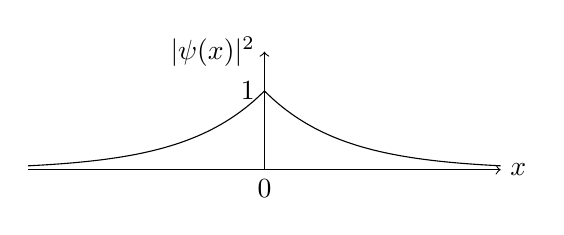
\begin{tikzpicture}
      \draw[->] (-3,0) -- (3,0) node[right] {$x$};
      \draw[->] (0,0) -- (0,1.5) node[left] {$|\psi(x)|^2$};
      \draw[domain=0:3,smooth,variable=\x,black] plot ({\x},{exp(-\x)});
       \draw[domain=-3:0,smooth,variable=\x,black] plot ({\x},{exp(\x)});
      \draw (0,0) node[below]{0};
\draw (0,1) node[left]{1};
\end{tikzpicture}
\hfill
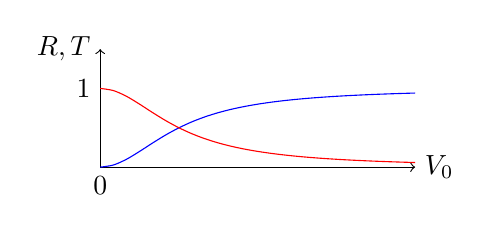
\begin{tikzpicture}
      \draw[->] (0,0) -- (4,0) node[right] {$V_0$};
      \draw[->] (0,0) -- (0,1.5) node[left] {$R,T$};
      \draw[domain=0:4,smooth,variable=\x,blue] plot ({\x},{\x^2/(\x^2+1)});
      \draw[domain=0:4,smooth,variable=\x,red] plot ({\x},{1/(\x^2+1))});
      \draw (0,0) node[below]{0};
\draw (0,1) node[left]{1};
\end{tikzpicture}
\end{center}
\end{enumerate}
\end{ans}
\newpage
\begin{qns}[Harmonic Oscillator]
A particle of mass $m$ moves in a one-dimensional potential $V(x)=\frac{1}{2}m\omega^2x^2$. The quantum mechanical ladder operators are defined by
$$\hat{a}=\sqrt{\frac{m\omega}{2\hbar}}\bigg(\hat{x}+i\frac{\hat{p}}{m\omega}\bigg)~\text{ and }~\hat{a}^\dag=\sqrt{\frac{m\omega}{2\hbar}}\bigg(\hat{x}-i\frac{\hat{p}}{m\omega}\bigg)$$
where $\hat{x}$ and $\hat{p}$ are the position and momentum operators, respectively.
\begin{enumerate}[label=(\roman*)]
\item Show that the Hamiltonian for the particle can be written as $\hat{H}=\hbar\omega(\hat{a}^\dag\hat{a}+0.5)$.\hfill\textbf{[3]}
\item Show further that $[\hat{a},\hat{a}^\dag]=1$ and $[\hat{H},\hat{a}]=-\hbar\omega\hat{a}$.\hfill\textbf{[4]}
\item If $|\phi_n\rangle$ is a normalised eigenstate of $\hat{H}$ , with energy $E_n=(n+0.5)\hbar\omega$, show that $\hat{a}|\phi_n\rangle=\sqrt{n}|\phi_{n-1}\rangle$ for integer $n > 0$, and briefly explain why $\hat{a}|\phi_0\rangle=0$.\hfill\textbf{[5]}\\[5pt]
A certain normalised quantum state of the system, depending on a complex parameter $\alpha$, has the form
$$|\chi_\alpha\rangle=e^{-0.5|\alpha|^2}\sum_{n=0}^\infty\frac{\alpha^n}{\sqrt{n!}}|\phi_n\rangle$$
\item Show that $\hat{a}|\chi_\alpha\rangle=\alpha|\chi_\alpha\rangle$.\hfill\textbf{[3]}
\item If the system is in the state $|\chi_\alpha\rangle$ at time $t = 0$, show that at a later time $t$ it is in the
state $e^{-0.5i\omega t}|\chi_\beta\rangle$, where $\beta=\alpha e^{-i\omega t}$.\hfill\textbf{[5]}
\end{enumerate}
\end{qns}
\begin{ans}\leavevmode
\begin{enumerate}[label=(\roman*)]
\item Evaluate $\hat{a}\hat{a}$:
$$\hat{a}^\dag\hat{a}=\bigg(\sqrt{\frac{m\omega}{2\hbar}}\hat{x}-i\frac{1}{\sqrt{2m\hbar\omega}}\hat{p}\bigg)\bigg(\sqrt{\frac{m\omega}{2\hbar}}\hat{x}+i\frac{1}{\sqrt{2m\hbar\omega}}\hat{p}\bigg)=\bigg(\frac{m\omega}{2\hbar}\hat{x}^2+\frac{1}{2m\hbar\omega}\hat{p}^2\bigg)+i[\hat{x},\hat{p}]\sqrt{\frac{m\omega}{2m2\hbar\hbar\omega}}$$
Then, $\hbar\omega(\hat{a}^\dag\hat{a}+0.5)=\frac{1}{2}m\omega^2\hat{x}^2+\frac{\hat{p}^2}{2m}$, which is consistent with the Hamiltonian of harmonic oscillator.
\item The commutators are
$$[\hat{a},\hat{a}^\dag]=\sqrt{\frac{m\omega}{2\hbar}}\frac{-i}{\sqrt{2m\hbar\omega}}[\hat{x},\hat{p}]+i\sqrt{\frac{m\omega}{2\hbar}}\frac{1}{\sqrt{2m\hbar\omega}}[\hat{p},\hat{x}]=\frac{2}{2\hbar}i\hbar(-i)=1$$
$$[\hat{H},\hat{a}]=\hbar\omega[\hat{a}^\dag\hat{a},\hat{a}]=\hbar\omega[\hat{a}^\dag,\hat{a}]\hat{a}=-\hbar\omega\hat{a}$$
\item Using the result of part (ii):
$$\hat{H}\hat{a}|\phi_n\rangle=(\hat{a}\hat{H}+[\hat{H},\hat{a}])|\phi_n\rangle=(\hat{a}\hat{H}-\hbar\omega\hat{a})|\phi_n\rangle=(E-\hbar\omega)\hat{a}|\phi_n\rangle$$
Thus, $\hat{a}|\phi_n\rangle$ is an eigenvector of $\hat{H}$ with eigenvalue $E-\hbar\omega$. The results suggests $\hat{a}|\phi_n\rangle\propto|\phi_{n-1}\rangle$ with proportionality constant $\alpha$, then taking the norm:
$$|\alpha|^2=\langle \phi_n|\hat{a}^\dag\hat{a}|\phi_n\rangle=\langle \phi_n|\frac{\hat{H}}{\hbar\omega}-\frac{1}{2}|\phi_n\rangle=\frac{E_n}{\hbar\omega}-0.5\implies|\alpha|=\sqrt{n}$$
Thus, $\hat{a}|\phi_n\rangle=\sqrt{n}|\phi_{n-1}\rangle$ and so if $\hat{a}|\phi_0\rangle\neq0$, then the energy can be lowered to the point where energy is negative, which is unphysical.
\item Take the action of $\hat{a}$ onto $|\chi_\alpha\rangle$:
$$e^{-0.5|\alpha|^2}\sum_{n=0}^\infty\frac{\alpha^n}{\sqrt{n!}}\hat{a}|\phi_n\rangle=e^{-0.5|\alpha|^2}\sum_{n=0}^\infty\frac{\alpha^n}{\sqrt{n!}}\sqrt{n}|\phi_{n-1}\rangle==e^{-0.5|\alpha|^2}\sum_{n=0}^\infty\frac{\alpha^n}{\sqrt{(n-1)!}}|\phi_{n-1}\rangle=\alpha|\chi_\alpha\rangle$$
\item Introducing time-dependence:
$$|\phi(t)\rangle=e^{-0.5|\alpha|^2}\sum_{n=0}^\infty\frac{\alpha^n}{\sqrt{n!}}e^{-i\omega t}(e^{-i\omega t})^n|\phi_n\rangle=e^{-i\omega t}|\chi_{\alpha e^{-i\omega t}}\rangle$$
where $\beta$ is shown to be $\alpha e^{-i\omega t}$, which differs only by a phase factor.
\end{enumerate}
\end{ans}
\begin{qns}[Central Potential]
For two particles of mass $m_1$ and $m_2$ with an interaction potential $V(r)$, where $r$ is the separation of the particles, the time-independent Schrodinger equation describing the relative motion of the two particles may be written as
$$-\frac{\hbar^2}{2\mu r^2}\frac{\partial}{\partial r}\bigg(r^2\frac{\partial\psi}{\partial r}\bigg)+\frac{1}{2\mu r^2}\hat{L}^2\psi+V(r)\psi=E\psi$$
where $\mu=\frac{m_1m_2}{m_1+m_2}$ is the reduced mass of the particles.
\begin{enumerate}[label=(\roman*)]
\item By substituting the form $\psi(r,\theta,\phi)=R(r)Y_{lm}(\theta,\phi)$ for the wavefunction into the above Schrodinger equation, show that the function $U(r)=rR(r)$ satisfies the equation\hfill\textbf{[4]}
$$-\frac{\hbar^2}{2\mu}\frac{d^2U}{dr^2}+\frac{l(l+1)\hbar^2}{2\mu r^2}U+V(r)U=EU$$
Consider the case in which the potential has the form $V(r) = -V_0$ (where $V_0 > 0$) for $r\leq a$ and $V = 0$ for $r > a$, and for which $-V_0<E<0$.
\item Explain briefly why the function $U(r)$ must satisfy the boundary conditions $U(0) = 0$ and $U(r)\rightarrow0$ as $r\rightarrow\infty$.\hfill\textbf{[2]}
\item For the case $l=0$ show that solutions $U(r)$ satisfying the above boundary conditions have the form 
$$U(r)=
\left\{
        \begin{array}{ll}
      A\sin kr & r\leq a\\
      Be^{-qr} & r>a
        \end{array}
    \right.$$ 
where $A$ and $B$ are arbitrary constants, and find expressions for $k$ and $q$.\hfill\textbf{[4]}
\item By imposing appropriate boundary conditions at $r = a$, show that $\tan(ka)=-k/q$.\hfill\textbf{[2]}
\item Hence show that there exists at least one bound state with $l=0$ provided that $V_0>\frac{\pi^2\hbar^2}{8\mu a^2}$.\hfill\textbf{[2]} 
\item  What is the condition on $V_0$ for there to be only one such bound state?\hfill\textbf{[2]}
\item The deuteron is a bound state of a proton and a neutron, which can be modelled using a potential of this form, with $a=2.1\times10^{-15}$ m. Find a lower limit for $V_0$ using the
inequality derived above.\hfill\textbf{[2]}
\item The value of $V_0$ that accounts for the observed binding energy of the deuteron is 33.5 MeV. Explain whether you would expect any bound excited states of the deuteron to exist.\hfill\textbf{[2]}
\end{enumerate}
\end{qns}
\begin{ans}\leavevmode
\begin{enumerate}[label=(\roman*)]
\item Use separation of variables $\psi(r,\theta,\phi)=R(r)Y_{lm}(\theta,\phi)$ and that $\hat{L}^2$ commutes with the spherically symmetric Hamiltonian (and thus share an eigenbasis), and so $\hat{L}^2\psi=l(l+1)\hbar^2\psi$, then
$$-\frac{\hbar^2}{2\mu}\frac{1}{r^2}\frac{d}{dr}\bigg(r^2\frac{dR}{dr}\bigg)+\frac{\hbar^2}{2\mu r^2}l(l+1)R+V(r)R=ER$$
but 
$$\frac{1}{r^2}\frac{d}{dr}r^2\frac{dR}{dr}=\frac{1}{r^2}\frac{d}{dr}(-U+\frac{dU}{dr}r)=\frac{d^2U}{dr^2}\frac{1}{r}$$
Multiply everything by $r$ and replace $rR$ with $U$, we get our desired equation
\item For $\psi$ to be normalizable, we require $R$ to be finite at $r=0$ and $R\rightarrow 0$ as $r\rightarrow\infty$. So, $U=rR$ must be zero at $r=0$ and $r=\infty$.
\item If $l=0$, we can ditch the $l(l+1)$ term.
\begin{itemize}
    \item For $r\leq a$: the Schrodinger equation is $\frac{d^2U}{dr^2}=-\frac{2\mu}{\hbar^2}(E+V_0)<0$ and so $U=A\sin(kr)$ since $U(0)=0$;
    \item For $r>a$: the Schrodinger equation is $\frac{d^2U}{dr^2}=-\frac{2\mu E}{\hbar^2}=\frac{2\mu|E|}{\hbar^2}>0$ and so $U=Be^{-qr}$ since $U\rightarrow 0$ as $r\rightarrow\infty$.
\end{itemize}
where $k=\sqrt{\frac{2\mu(V_0+E)}{\hbar^2}}$ and $q=\sqrt{\frac{2\mu|E|}{\hbar^2}}$.
\item The boundary conditions at $r=a$ are
\begin{itemize}
    \item $U(r)$ is continuous at $r=a$: $A\sin(ka)=Be^{-qa}$;
    \item $\frac{dU(r)}{dr}$ is continuous at $r=a$: $kA\cos(ka)=-qBe^{-qa}$.
\end{itemize}
Together, this give $\tan(ka)=-k/q$.
\item The first intersection for these two graphs occur beyond the first positive vertical asymptote of $\tan$ for $ka>\frac{\pi}{2}$:
$$k^2a^2>\frac{\pi^2}{4}\implies V_0+E>V_0>\frac{\pi^2\hbar^2}{8\mu a^2}$$
where $-V_0<E<0$.
\item For only one bound state, $\frac{3\pi}{2}>ka>\frac{\pi}{2}$,
$$\frac{9\pi^2}{4}>\frac{2\mu(V_0+E)a^2}{\hbar^2}\implies V_0+E<\frac{9\hbar^2\pi^2}{8\mu a^2}$$
the lower bound is found earlier in part (v) to be $$V_0>\frac{(6.626\times10^{-34}/2\pi)^2\pi^2}{8(1.67\times10^{-27}/2)(2.1\times10^{-15})^2}=24 \text{MeV}$$
\item Since $V_0<9\times 24=219$ MeV, there is only one bound state and no bound excited states. 
\end{enumerate}
\end{ans}
\newpage
\begin{qns}[Identical Particles]\leavevmode
\begin{enumerate}[label=(\roman*)]
\item Write down the time-dependent Schrodinger equation satisfied by the two-particle wavefunction $\Psi(\mathbf{r_1},\mathbf{r_2},t)$ for two non-interacting, distinguishable particles, each of mass $m$, moving in some potential $V$, where $\mathbf{r_1}$ and $\mathbf{r_2}$ are the positions of the two particles.\hfill\textbf{[2]}
\item Show that the equation is satisfied by the two-particle wavefunction
$$\Psi(\mathbf{r_1},\mathbf{r_2},t)=\phi_a(\mathbf{r_1})\phi_b(\mathbf{r_2})e^{-iEt/\hbar}$$
where $\phi_a(\mathbf{r_1})$ and $\phi_b(\mathbf{r_2})$ are single-particle stationary states and $E$ is the total energy of the particles.\hfill\textbf{[4]}
\item Suppose now that the particles are indistinguishable with spin $\frac{1}{2}$. Discuss how the form of the two-particle wavefunction must be modified and write down the various possibilities that are the product of a spatial and a spin part.\hfill\textbf{[5]}
\item What are the total spin quantum numbers $S$ and $m_S$ corresponding to each of your two-particle wavefunctions?\hfill\textbf{[4]}
\item If there is a small Coulomb repulsion between the particles, which state or states are likely to have the lower energy?\hfill\textbf{[2]}
\item Suppose instead that the particles are non-interacting and indistinguishable with spin 0. Calculate the factor by which the probability of finding two such particles at the same position is enhanced relative to that for two distinguishable particles.\hfill\textbf{[3]}
\end{enumerate}
\end{qns}
\begin{ans}\leavevmode
\begin{enumerate}[label=(\roman*)]
\item The time-independent Schrodigner equation is
$$\bigg(-\frac{\hbar^2}{2m}\nabla^2_{\mathbf{r_1}}+V-\frac{\hbar^2}{2m}\nabla^2_{\mathbf{r_2}}+V\bigg)\Psi(\mathbf{r_1},\mathbf{r_2},t)=E\Psi(\mathbf{r_1},\mathbf{r_2},t)$$
\item Assume the single particle states satisfy $-\frac{\hbar^2}{2m}\nabla^2\phi_{a,b}(\mathbf{r_{1,2}})+V\phi_{a,b}(\mathbf{r_{1,2}})=E_{a,b}\phi_{a,b}(\mathbf{r_{1,2}})$ and suppose $\Psi(\mathbf{r_1},\mathbf{r_2},t)$ has the given form, then we can decouple the result in part (i) to get $E=E_a+E_b$, as expected.
\item The spin-$\frac{1}{2}$ particles are fermions by the Spin-Statistics Theorem and thus odd symmetry under exchange. Rewrite $\Psi$ as
$$\Psi(\mathbf{r_1},\mathbf{r_2},t)=\frac{1}{\sqrt{2}}(\phi_a(\mathbf{r_1}\phi_b(\mathbf{r_2})-\phi_a(\mathbf{r_2}\phi_b(\mathbf{r_1}))e^{-iEt/\hbar}=-\Psi(\mathbf{r_2},\mathbf{r_1},t)$$
which is odd under exchange of $\mathbf{r_1}$ and $\mathbf{r_2}$. We can further decompose into spatial and spin parts, i.e. $\phi_{a,b}=\Phi_{a,b}\chi_{\alpha,\beta}$, then
$$\Psi=\frac{1}{\sqrt{2}}(\phi_a(\mathbf{r_1}\phi_b(\mathbf{r_2})-\phi_a(\mathbf{r_2}\phi_b(\mathbf{r_1}))e^{-iEt/\hbar}\frac{1}{\sqrt{2}}(\chi_\alpha(1)\chi_\beta(2)\mp\chi_\alpha(2)\chi_\beta(1))$$
Either parts must be anti-symmetric for $\psi$ to be odd.
\item The symmetric spin wavefunction has total $S=1$ and degeneracy of 3, i.e. $m_S=-1,0,1$. The anti-symmetric spin wavefunction has total $S=0$ and $m_S=0$.
\item For a small Coulomb repulsion, the state with the smallest spatial separation will have the largest energy increase, so the anti-symmetric spatial state (and hence symmetric spin from part (iii) will have lower energy.
\item With spin 0, then from part (iv), the spin wavefunction must be anti-symmetric and the spatial part must be symmetric, i.e.
$$\Psi=\frac{1}{\sqrt{2}}(\Phi_a(\mathbf{r_1})\Phi_b(\mathbf{r_2})+\Phi_a(\mathbf{r_2})\Phi_b(\mathbf{r_1}))e^{-iEt/\hbar}$$
Compare with distinguishable case, $\Psi=\Phi_a(\mathbf{r_1})\Phi_b(\mathbf{r_2})$, then the relative probabilities of finding in the saem location is $|2/\sqrt{2}|^2=2$.
\end{enumerate}
\end{ans}
\newpage
\subsubsection{Section C}
\begin{qns}[QM Essay]
Write an essay on angular momentum in quantum mechanics, including a discussion of orbital and spin angular momentum and the Stern–Gerlach experiment.

\hfill\textbf{[20]}
\end{qns}
\begin{ans}
Generic rotations in quantum physics are described by the angular momentum operator $\mathbf{J}$, which was originally thought of as a sum of the orbital angular momentum $\mathbf{L}$ (translate an object's centre of mass along a circular arc) and spin $\mathbf{S}$ (which was originally thought as self-rotation about its own centre of mass). While the operator actions are identical for both, it turns out spin is due to an intrinsic property, inherent to quantum particles and unrelated to the classical notion of `self-rotation'.\\[5pt]
Suppose we translate our system around an $N$-sided regular polygon. As $N\rightarrow\infty$, this will be a circular translation. The orbital angular momentum operator $\mathbf{L}$ is a generator of this circular translation. If our system is initially located at some $\mathbf{x}\in\mathbb{R}^3$, then we translate it through $\delta\mathbf{a}=\delta\alpha\mathbf{n}\times\mathbf{x}$, where $\mathbf{n}$ is the unit normal to the plane of the polygon. Hence, our translation is
$$U(\delta\mathbf{a})^{-1}\mathbf{X}U(\delta\mathbf{a})=\mathbf{X}+\delta\alpha(\mathbf{n}\times\mathbf{X})$$
where $\mathbf{X}$ is the position operator and $U(\delta\mathbf{a})$ is the associated unitary translation operator, which is (discarding second order terms in $\delta\alpha^2$)
$$U(\delta\mathbf{a})=1-\frac{i}{\hbar}\delta\mathbf{a}\cdot\mathbf{P}=1-\frac{i}{\hbar}\delta\alpha(\mathbf{n}\times\mathbf{X})\cdot\mathbf{P}=1-\frac{i}{\hbar}\delta\boldsymbol{\alpha}\cdot(\mathbf{X}\times\mathbf{P})$$
where $\mathbf{P}$ is the momentum operator, and we identify $\mathbf{L}=\mathbf{X}\times\mathbf{P}$ which is a Hermitian operator by inspection, and thus corresponds to the angular momentum observable. Classically,  $\mathbf{L}=\mathbf{r}\times\mathbf{p}=\epsilon_{ijk}x_ip_j\mathbf{\hat{k}}$. The corresponding quantum mechanial definition is
$$\mathbf{\hat{L}_i}=-i\hbar\epsilon_{jki}\mathbf{\hat{x}_j}\frac{\partial}{\partial x_k}$$ 
The total angular momentum operator will then be 
$$\mathbf{\hat{L}^2}=\mathbf{\hat{L}_i}\mathbf{\hat{L}_i}$$
One can show that the angular momentum operators satisfy the following commutators:
$$[\mathbf{\hat{L}_i},\mathbf{\hat{L}_j}]=i\hbar\epsilon_{ijk}\mathbf{\hat{L}_k},\quad [\hat{L}^2,\mathbf{\hat{L}_i}]=0$$
The fact that the angular momentum operators along any two distinct directions do not commute would mean that we are not able to simultaneously measure the angular momentum in all three directions. Fortunately, we can simultaneously determine the total angular momentum and the angular momentum in any one direction. This non-commutativity would mean that the angular momentum operators satisfy the uncertainty principle
$$\sigma_{L_x}\sigma_{L_y}\geq\frac{\hbar^2}{2}|\langle\mathbf{\hat{L}_z}\rangle|$$
Geometrically, the angular momentum vector $L$ traces out a cone in 3 dimensional angular momentum space where the length of the vector is $\hbar\sqrt{l(l+1)}$ and the half angle of the cone is $\cos^{-1}(m/\sqrt{l(l+1)})$.  $m$ is thus the projection of the angular momentum vector along the $z$ axis. As the angular momenta states are quantized, $\theta$ is quantized too and have a discrete set of $2l + 1$ possible values. As $l\rightarrow\infty$ (classical limit), $\theta\rightarrow 0$, this physically means we can measure the angular momentum's direction with great certainty, consistent with the correspondence principle.\\[5pt]
Since $[\hat{L}^2,\mathbf{\hat{L}_i}]=0$, we can define a simultaneous eigenstate. Without loss of generality, choose the $z$ direction. Then, let's assume the simultaneous state $\{|\beta,m\rangle\}$ (properly normalized, orthonormal and non-degenerate) obeys
$$\hat{L}^2|\beta,m\rangle=\beta\hbar^2|\beta,m\rangle,\quad \mathbf{\hat{L}_z}|\beta,m\rangle=m\hbar|\beta,m\rangle$$
One can proceed to show that the eigenvalues of $\mathbf{\hat{L}}^2$ are of the form $\hbar^2l(l+1)$ with $l$ integer or half-integer. Furthermore, for a given value of $l$, the eigenvalues of $\mathbf{\hat{L}_z}$ are $\hbar m$ with $m\in\{-l,-l+1,...,l-1,l\}$. That is, the eigenvalue $l$ of $\mathbf{L}^2$ has a multiplicity of $2l+1$. $l$ and $m$ are known as the orbital angular momentum quantum number and zimuthal quantum number respectively.\\[5pt]
One can then define ladder operators to relate states of the same angular momentum number $l$, i.e. For $m=-l$, $\mathbf{\hat{L}_-}|l,m\rangle=0$. If $m>-l$, we obtain $|l,m-1\rangle$ after one iteration of $\mathbf{\hat{L}_-}$. Similarly, for $m=+l$, $\mathbf{\hat{L}_+}|l,m\rangle=0$. If $m<l$, we obtain $|l,m-1\rangle$. By normalizing the resultant state, one can show 
$$\mathbf{\hat{L}_\pm}|l,m\rangle=\hbar\sqrt{l(l+1)-m(m\pm1)}|l,m\pm1\rangle$$
In fact, the commutator $[\mathbf{\hat{L}_i},\mathbf{\hat{L}_j}]=i\hbar\epsilon_{ijk}\mathbf{\hat{L}_k}$ suggests that we can represent the actions of the angular momentum operators as finite-dimensional matrices (we can't do this for position and momentum operators). The matrix representations will be $$\langle l',m'|\mathbf{\hat{L}^2}|l,m\rangle=\hbar^2l(l+1)\delta_{l',l}\delta_{m',m}$$
$$\langle l',m'|\mathbf{\hat{L}_z}|l,m\rangle=\hbar m\delta_{l',l}\delta_{m',m}$$
$$\langle l',m'|\mathbf{\hat{L}_x}|l,m\rangle=0.5\hbar[\sqrt{l(l+1)-m(m+1)}\delta_{m',m+1}+\sqrt{l(l+1)-m(m-1)}\delta_{m',m-1}]\delta_{j',j}$$
$$\langle l',m'|\mathbf{\hat{L}_y}|l,m\rangle=0.5\hbar[\sqrt{l(l+1)-m(m+1)}\delta_{m',m+1}-\sqrt{l(l+1)-m(m-1)}\delta_{m',m-1}]\delta_{j',j}$$
Finally, if a physical quantity $A$ is rotational invariant, it commutes with the angular momentum, i.e. $[\mathbf{\hat{A}},\mathbf{\hat{L}}]=0$. All the operator algebra discussed is still relevant for spin. Below we outline the famous Stern-Gerlach experiment to motivate the revolutionary idea of quantum spin.\\[5pt]
In 1922, Otto Stern and Walther Gerlach devised an experiment to investigate whether angular momentum is quantized. A beam of neutral Ag atoms (in the ground state such that total angular momentum is zero since the valence electron is in 5s orbital) are passed through the poles of a long magnet (non-uniform magnetic field between the pole pieces but uniform along the length of the magnet). In this experiment, a beam of Ag atoms each of mass $m$ was sent through a region of varying $\mathbf{B}$ field. The Hamiltonian is 
$$H=\frac{\hat{p}^2}{2m}-\boldsymbol{\mu}\cdot\mathbf{B}(\mathbf{\hat{x}})$$
where $\boldsymbol{\mu}$ is the magnetic dipole moment, which is non-zero since atoms have non-trivial spin $s$, i.e. $\boldsymbol{\mu}=\frac{\mu}{\hbar s}\mathbf{\hat{S}}$ where without loss of generality, we choose our axes for the magnetic field to be $\mathbf{B}=B(\mathbf{\hat{x}})\mathbf{\hat{z}}$. The equation of motion from the Heisenberg picture gives
$$\frac{d\langle\mathbf{\hat{x}}\rangle}{dt}=\frac{\langle\mathbf{\hat{p}}\rangle}{m},\quad \frac{d\langle\mathbf{\hat{p}}\rangle}{dt}=\frac{\mu}{\hbar s}\langle\boldsymbol{\nabla}B \hat{S}_z\rangle$$
Atoms experience a force from the non-uniform $B$ field in the $\perp$ direction, depending on their spin state $|s,\sigma\rangle$. If a given atom is in state $|s,s\rangle$ with spin aligned along the direction of $\mathbf{B}$, then it will be driven towards increasing $|\mathbf{B}|$ whereas $|s,-s\rangle$ will be driven away from this region. Classically, a continuous range of outcomes is possible, whereas quantum mechanically, only a limited number of discrete momenta are possible, whereas in quantum mechanics, since the atomic spins are initially randomly aligned, we would expect our beam to be deflected into $2s+1$ separate paths. But Stern Gerlach observed just two different paths for Ag atoms, hence Ag atoms have $s=0.5$.\\[5pt]
The half-integer angular momenta is incompatible with our classical idea of spin - self-rotation (which was originally thought to be the difference between angular momentum $J$ and orbital angular momentum $L$). Originally, it was suggested in early 1925 that spin was due to self-rotation. When Pauli heard about the idea, he criticized it severely, noting that for an electron to have half-integer spin, the electron's hypothetical surface would have to be moving faster than the speed of light in order for it to rotate quickly enough to produce the necessary angular momentum. This would violate the theory of relativity. Hence, spin is an intrinsic property inherent to quantum particles and here, these particles are not self-rotating (thus no classical analogue).
\end{ans}
\newpage
\begin{qns}[QM Short Notes]
Write brief notes on two of the following:\hfill\textbf{[20]}
\begin{itemize}
    \item Bohr’s model of the atom;
    \item Ehrenfest’s theorem and the correspondence principle;
    \item the properties of Hermitian operators and their role in quantum mechanics.
\end{itemize}
\end{qns}
\begin{ans}\leavevmode
\subsubsection*{Bohr's model of the atom}
In 1911, Rutherford proposed an atomic model, which was inspired by the orbiting motion of planets around the Sun, that consists of electrons orbiting a positively charged nucleus. The classical contradiction is
\begin{itemize}
\item Using Maxwell's electromagnetic theory on Rutherford's model, the electron accelerates with acceleration $a$ and radiates energy. The magnitude of this radiated energy is given by the Larmor formula (from electrodynamics).
$$\frac{dE}{dt}=-\frac{2}{3}\frac{e^2a^2}{4\pi\epsilon_0c^3}$$
By balancing Coulomb's electric force and centripetal force, the rate of change of energy of the electron is 
$$\frac{dE}{dt}=\frac{d}{dt}\bigg(\frac{1}{2}m\frac{1}{4\pi\epsilon_0}\frac{e^2}{mr}-\frac{1}{4\pi\epsilon_0}\frac{e^2}{r}\bigg)=-\frac{d}{dt}\frac{1}{4\pi\epsilon_0}\frac{e^2}{2r}=\frac{1}{4\pi\epsilon_0}\frac{e^2}{2r^2}\frac{dr}{dt}$$
Equating them such that $a$ is $\frac{1}{4\pi\epsilon_0}\frac{e^2}{mr^2}$ and was obtained from Coulomb's Law. We will thus obtain a differential equation for $\frac{dr}{dt}=-(\frac{1}{4\pi\epsilon_0})^2\frac{4}{3}\frac{e^4}{m^2r^2c^3}$. For the electron (with initial radius $r$) to spiral and crash into the nucleus, the time taken will be
$T=\frac{m^2c^3}{4e^4}(4\pi\epsilon_0)^2r^3$. 
This value is alarmingly small, to the power of $-10$. Yet, atoms are surprisingly stable and contradicts with classical theory.
\item Since the frequency of the radiated energy is the same as the orbiting frequency, and as the electron orbit collapses, its orbiting frequency increases continuously. Hence, the spectrum of the radiation emitted by the atom should be continuous. Yet, atomic spectra are found to be discrete. Examples include Lyman series (UV light, from ground state), Balmer series (visible light, from first excited state) and Paschen series (infrared, from second excited state).
\end{itemize}
Inspired by Planck's postulate, Bohr proposed in 1913 a model where the electron's energy is quantized and only fill a discrete set of circular stable orbits. These allowed orbits also correspond to quantized orbital angular momentum, where $L=n\hbar$.\\[5pt]
Moreover, as long as an electron remains in one of these stationary orbits, it will not radiate electromagnetic energy. Emission or absorption of radiation can take place only when an electron jumps from one allowed orbit to another. Hence $hf=E_n-E_m$ represents the energy of radiation emitted when the electron transits from the nth orbit to the $m$th orbit.\\[5pt]
We will consider a hydrogen atom $(Z=1)$. Similar to how we calculate the time for radiative collapse of an atom, we will equate the centripetal force and the electrostatic force of the electron. The radius of these quantized orbits is thus  $r_n=(\frac{4\pi\epsilon_0\hbar^2}{m_ee^2})n^2$. 
The quantity $\frac{4\pi\epsilon_0\hbar^2}{m_ee^2}$ is defined as the Bohr radius which is $0.053$ nm. The orbital velocity of these quantized orbits is $
v_n=(\frac{e^2}{4\pi\epsilon_0})\frac{1}{n\hbar}$. 
The fine structure constant, $\alpha$ is defined to be the ratio between the speed of the electron in the first Bohr orbit to the speed of light.
$$\alpha=\frac{v_1}{c}=\frac{1}{4\pi\epsilon_0}\frac{e^2}{\hbar c}=\frac{1}{137}\implies E_n=-\frac{e^2}{8\pi\epsilon_0}\frac{1}{r_n}=-\frac{m_e}{2\hbar^2}\bigg(\frac{e^2}{4\pi\epsilon_0}\bigg)^2\frac{1}{n^2}$$
The quantity $\frac{m_e}{2\hbar^2}(\frac{e^2}{4\pi\epsilon_0})^2$ is called Rydberg constant, which is 13.6eV. This is also the ionization energy of the Hydrogen atom, amount of energy to bring the electron in the first Bohr orbit to infinity. 
\subsubsection*{Ehrenfest's theorem and the correspondence principle}
Correspondence Principle states that in the macroscopic/classical limit where we consider large principle quantum numbers, the results of any quantum problem should match with that of the corresponding classical problem.\\[5pt]
Consider the example of a finite square well. If $E\rightarrow\infty$, the beam of particles will not feel the effects of the potential. Classically, we expect complete transmission. Quantum mechanically, the transmission probability is
$$T=\frac{4k_1^2k_2^2}{4k_1^2k_2^2\cos^2(k_2a)+(k_1^2+k_2^2)\sin^2(k_2a)},\quad\lim_{E\rightarrow\infty}T=1$$
For the example of an infinite square well, in the limit of $n\rightarrow\infty$, we would classically expect a variance of $\sigma_x^2=a^2/12$. This is because the classical probability distribution is uniform, i.e. $f(x)=\frac{1}{a},\quad 0\leq x\leq a$. The variance would be
$$\sigma_x^2=E[X^2]-\mu^2=\int_0^a\frac{x^2}{a}dx-\bigg(\int_0^a\frac{x}{a}\bigg)^2=\frac{a^2}{12}$$
Quantum mechanically, we have the variance in $x$ to be the squared of the uncertainty
$$\sigma_x^2=\langle x^2\rangle-\langle x\rangle^2=\frac{1}{a}\int_0^ax^2\bigg(1-\cos^2\frac{n\pi x}{a}\bigg)dx-\bigg(\int_0^a\frac{2}{a}x\sin^2\frac{n\pi x}{a}dx\bigg)^2=a^2\bigg(\frac{1}{12}-\frac{1}{2n^2\pi^2}\rightarrow\frac{a^2}{12}\bigg)~\text{ as }~n\rightarrow\infty$$
The classical probability distribution for a one-dimensional harmonic oscillator in the interval $|x|<A$ is
$$P_{\text{cl}}=\frac{2dt}{T}=\frac{2dx}{Tv}=\frac{2dx}{T\omega\sqrt{A^2-x^2}}=\frac{dx}{\pi\sqrt{A^2-x^2}}$$
where $x=A\cos\omega t$. For large $n$, the norm of the wavefunction $|\psi_{n\rightarrow\infty}|^2$ will have asymptotic behaviour similar to the classical distribution, where the probability for the particle to be at $x=\pm a$ is significantly higher.\\[5pt]
In the topic of angular momentum, we see that since $[J_i,J_j]\neq 0$ for $i\neq j$, we cannot simultaneously measure the angular momentum in any two directions. But yet, $[J^2,J_i]=0$ $\forall i$, so we can simultaneously measure the total angular momentum and the angular momentum along any direction. In $J$-space, this is represented by a cone where the half-angle of the cone $\theta$ is $\theta=\cos^{-1}\frac{j_z}{j^2}$, where $j_z$ and $j^2$ are the eigenvalues of the operators $J_z$ and $J^2$ on a simultaneous eigenstate. In the limit of large quantum numbers $j\rightarrow\infty$, this angle $\theta\rightarrow 0$. Classically, this is expected since we can definitely simultaneously measure both the angular momentum magnitude and direction.\\[5pt]
Lastly, one recovers the classical dynamical equations of motion when we take the time derivative of the expectation of the corresponding quantum observables. In general, this is obtained from the Ehrenfest's theorem for a generic quantum observable $Q$. 
$$i\hbar\frac{d}{dt}\langle Q\rangle_\psi=\langle [Q,H]\rangle_\Psi+i\hbar\langle\dot{Q}\rangle_\Psi$$
This follows from the definition of expectation and Schr\"{o}dinger's equation. In quantum mechanics, we note that the commutators for a free particle of Hamiltonian $H=\frac{p^2}{2m}+V(x)$ are $[x,H]=\frac{i\hbar}{m}p$ and $[p,H]=-i\hbar V'(x)$.
$$\frac{d}{dt}\langle x\rangle_\Psi=\frac{1}{m}\langle p\rangle_\Psi,\quad\frac{d}{dt}\langle p\rangle_\Psi=-\langle V'(x)\rangle_\Psi$$
which is consistent with the classical counterparts - the Newtonian equations of motion. \\[5pt]
Other examples include
\begin{itemize}
    \item Planck radiation law to converge to Rayleigh-Jeans law when $\hbar\rightarrow 0$
    \item Bohr's model in the limit of $n\rightarrow\infty$ has a spectrum consistent with the classical continuum
    \item Feynman reformulate quantum mechanics (quantum field theory) as extensions of Hamilton's principle of least action (in classical mechanics).
\end{itemize}
See \url{https://physicstoday.scitation.org/doi/pdf/10.1063/1.2916084}
\subsubsection*{The properties of Hermitian operators and their role in quantum mechanics}
An observable is a measurable property of the system. Each observable is represented by a Hermitian operator acting on the wavefunction of the system. Let $Q$ be a Hermitian operator, then
\begin{enumerate}
    \item the eigenvalues of $Q$ are real,
    \item the eigenstates of $Q$ with different eigenvalues are orthogonal with respect to the complex inner product.
\end{enumerate}
For most operators, the set of eigenstates is complete.\\[5pt]
Hermitian operators are fundamental in our understanding of quantum mechanics, where the measurement postulate is key to all quantum systems. Consider an observable $A$ with discrete spectrum and normalized eigenstates. We can decompose any state $\psi=\sum_n\alpha_n\chi_n$ with $A\chi_n=\lambda_n\chi_n$ and $\langle\chi_m,\chi_n\rangle=\delta_{mn}$ such that $\alpha_n=\langle\chi_n,\psi\rangle$. The outcome of a measurement is some eigenvalue of $Q$ and the probability of obtaining $\lambda_n$ is $P_n=|\alpha_n|^2$ where $\alpha_n=\langle\chi_n,\psi\rangle$ is the amplitude. The state $\psi$ collapses to $\chi_n$ immediately after a measurement outcome of $\alpha_n$. The measurement axiom is consistent to the normalization condition on $\psi$.
$$\langle\psi,\psi\rangle=\bigg\langle\sum_m\alpha_m\chi_m,\sum_n\alpha_n\chi_n\bigg\rangle=\sum_{m,n}\alpha_m^*\alpha_n\langle\chi_m,\chi_n\rangle=\sum_n|\alpha_n|^2$$
where we used the fact that eigenstates with distinct eigenvalues are orthogonal. RHS has to be 1 since the sum of all probabilities is 1 (probability axiom). Then LHS is the normalization condition.\\[5pt]
More importantly, the evolution of any quantum system relies on the Stone's theorem, which states any unitary operator can be expressed as $U=e^{iH}$ where $H$ is Hermitian. Any evolution from one state to another must be unitary to ensure normalization of the state after the transformation.
$$1=\langle\psi'|\psi'\rangle=\langle\psi|U^\dag U|\psi\rangle$$
One important application of unitary evolution is time evolution. By treating time evolution as a unitary operator, we can obtain the time-dependent Schr\"{o}dinger's equation. We write $U(t)=e^{-iHt/\hbar}$ and we have $|\psi(t)\rangle=U(t)|\psi(0)\rangle$ and hence
$$|\psi(t+\delta t)\rangle-|\psi(t)\rangle=[U(t+\delta t)-U(t)]|\psi(0)\rangle=(U(\delta t)-1)U(t)|\psi(0)\rangle=\bigg(1-i\frac{\delta t}{\hbar}H-1\bigg)|\psi(t)\rangle$$
or equivalently, $i\hbar\frac{\partial}{\partial t}|\psi(t)\rangle=H(t)|\psi(t)\rangle$, which is the time-dependent Schr\"{o}dinger's equation.
\end{ans}
\newpage
\subsubsection{Section D}
\begin{qns}[Sampling]
A harmonic oscillator at finite temperature is undergoing overdamped Brownian motion. In the frequency domain, the ideal spectral density $P_i(f)$ of the fluctuations is directly proportional to
$$\frac{1}{f^2+f_c^2}$$
where $f$ is the frequency of the fluctuations and $f_c$ is the characteristic frequency determined by the harmonic potential.
\begin{enumerate}[label=(\roman*)]
\item Sketch $P_i(f)$ on a log-log plot for two different values of $f_c$.\hfill\textbf{[4]}\\[5pt]
The fluctuations of the oscillator are detected with a position-sensitive detector. An electronic circuit based on an operational amplifier is used to convert the current from the detector into a voltage signal that is digitised with an analogue-to-digital converter. The measured spectral density $P_m(f)$ from the detector yields the following results:
\begin{center}
\begin{tabular}{|c|c|}
\hline
Frequency (Hz) & $P_m(f)$ (V$^2$ Hz$^{-1}$)\\
\hline
0.01 & $1\times10^{-4}$\\
0.1 & $1\times10^{-5}$\\
1.0 & $1\times10^{-6}$\\
10 & $1\times10^{-6}$\\
100 & $1\times10^{-6}$\\
1000 & $5\times10^{-7}$\\
10000 & $1\times10^{-8}$\\
100000 & $1\times10^{-10}$\\
1000000 & $1\times10^{-15}$\\
\hline
\end{tabular}
\end{center}
\item Plot $P_m(f)$ on log-log axes and use your plot over the frequency range 1 Hz to $10^5$ Hz to estimate the value of $f_c$ graphically.\hfill\textbf{[6]}
\item Describe how $P_m(f)$ differs from $P_i(f)$ at $f<<f_c$ and comment briefly on the behaviour. What is the minimum recording time required to record the lowest-frequency data point?\hfill\textbf{[3]}
\item What is the minimum sampling rate required to obtain $P_m(f)$?\hfill\textbf{[2]}
\item Describe how $P_m(f)$ deviates from $P_i(f)$ at high frequencies. Comment on why, in general, an amplifier might be designed such that its gain rolls off at high frequencies.\hfill\textbf{[5]}
\end{enumerate}
\end{qns}
\begin{ans}\leavevmode
\begin{enumerate}[label=(\roman*)]
\item We have
$$P_i(f)=\frac{C}{f_c^2}\bigg(1+\bigg(\frac{f}{f_c}\bigg)^2\bigg)^{-1}\implies\ln P_i(f)=\ln\frac{C}{f_c^2}-\ln\bigg(1+e^{-2\ln f_c}e^{2\ln f}\bigg)$$
At small frequencies, $f<<f_c$, we have $\ln(1+e^{2\ln(f/f_c)})\approx e^{2\ln(f/f_c)}$, which decays rapidly to zero. Hence, $\ln P_i(f)$ approximately a constant. On the other hand, at large frequencies, $f>>f_c$, we have $\ln(1+e^{2\ln(f/f_c)})\approx2\ln\frac{f}{f_c}$, i.e. a straight line of negative gradient of $-2$. The transition is gradual and smooth, at roughly $f\sim f_c$.
\begin{figure}[H]
    \centering
    \includegraphics[scale=0.5]{2017P1D12i.PNG}
    \caption{Plot $\ln P(f)$ against $\ln f$ - for large $f_c$ (orange) and small $f_c$ (blue).}
\end{figure}
\item Plot $\ln P_m(f)$ against $\ln(f)$. Over the given frequency range, we realize the graph is similar to the sketch in part (i). Thus, $f_c\sim 10^3$ Hz.
\begin{figure}[H]
    \centering
    \includegraphics[scale=0.75]{2017P1D12ii.PNG}
    \caption{Plot $\ln P_m(f)$ against $\ln f$. Extrapolate two lines to determine $f_c$. The gradient for the grey and orange lines are respectively 0 and $-2$ exactly.}
\end{figure}
\item $P_m$ is consistent with $P_i$ for $f<<f_c$ and seems to have a $P\sim f^{-1}$ behaviour. The minimum time to record the lowest frequency signal is given by Nyquist theorem which predicts we need to use a frequency of $2 \times 0.01$ Hz, which corresponds to a time of 50 seconds.
\item To obtain the full spectrum we need to sample at twice the maximum
frequency in the entire signal (by Nyquist Theorem), so at 2 MHz.
\item At high frequencies, the measured frequency is much lower than predicted, as seen in the last blue data point. This is because real operational amplifiers have a non zero time delay. At high frequencies this is equivalent to larger and larger phase shifts. As the operational amplifier is used with negative feedback to provide stability, a phase shift comparable to $\pi/2$ would undesirably turn negative feedback into positive feedback. To avoid this, the operational amplifier has an internal frequency compensation that ensures the amplitude to fall off rapidly, before attaining a critical frequency.
\end{enumerate}
\end{ans}
\newpage
\begin{qns}
Write brief notes on two of the following:\hfill\textbf{[20]}
\begin{itemize}
    \item reducing noise in electrical circuits;
    \item Nyquist’s theorem and digital sampling;
    \item the importance of Gaussian distributions in experimental physics.
\end{itemize}
\end{qns}
\begin{ans}\leavevmode
\subsubsection*{Reducing noise in electrical circuits:}
There are various types of noises in electrical circuits. These are undesirable since it distorts electrical signals, in turn giving inaccurate data and measurements. Generally, noise can occur extrinsically or intrinsically.\\[5pt]
To shield against external electric fields, use a Faraday cage. To shield against external magnetic field, we use a high permeability metal to provide a low reluctance path for B field lines. If the cables generate these stray magnetic fields, one may use twisted pair wires. Coaxial cables may also be used for better shielding.\\[5pt]
On the other hand, intrinsic noise in electrical circuits are $1/f$ noise, Johnson noise and shot noise.\\[5pt]
$1/f$ noise is generally the most significant contribution to noise (except interference). It depends a good deal on the construction of the components and the quality of the contacts. It can, unlike shot and Johnson noise as discussed later, be reduced by careful choice of components. Its power spectrum is proportional to $1/f$. Given this dependence, the noise energy per frequency decade (rather than per unit frequency) is constant over the spectrum (over which the noise extends). This type of noise spectrum is called pink noise.\\[5pt]
Johnson noise is the thermally induced noise that is present in any resistive element. It is the electronic analogue of the random motion of gas molecules in a box, which is known as Brownian motion. In noise terminology, Johnson noise is white noise which is noise power per unit frequency that is independent of frequency, i.e. flat frequency spectrum. In fact, the Johnson noise is independent of the design of the resistive elements, and represents noise we could never eliminate. Of course, Johnson noise could be eliminated in a superconducting electrical circuit.\\[5pt]
Shot Noise (white noise) is present in any circuit that carries a current. Its relative importance varies inversely with current. A current $I$ consists of a flow of electrons of the form $I=e\langle N\rangle$, where $\langle N\rangle$ is the average number of electrons passing through a plane normal to the electron flow per unit time. However, during any given time interval, not necessarily exactly $\langle N\rangle$ electrons will pass the reference point. The distribution about $\langle N\rangle$ is given by $\langle N\rangle^{0.5}$, as for any statistical process (Poissonian distribution). This noise is a direct result of the quantization of the electric change and is given by r.m.s. value $\sqrt{2eIN}$. 
\subsubsection*{Nyquist's theorem and digital sampling:}
We discuss Nyquist's theorem and digital sampling in the context of digitally recording analogue data. An analog-to-digital converter (ADC) can be modeled as two processes: sampling and quantization.\\[5pt]
Sampling is to reduce a continuous time signal to a discrete time signal. This considerably reduces the data volume and appropriate for non-linear media. Sampled data are also easier to transmit without loss.\\[5pt]
Quantization replaces each real number with an approximation from a finite set of discrete values. Quantizing a sequence of numbers produces a sequence of quantization errors which is sometimes modeled as an additive random signal called quantization noise because of its stochastic behavior. The more levels a quantizer uses, the lower is its quantization noise power. But sampling the signal with finer resolution in amplitude (more signal levels) does not allow the sampling frequency to be reduced, i.e. no impact on Nyquist's theorem.\\[5pt]
Nyquist's Sampling Theorem states that, for a band-limited function, you need to sample at a minimum rate of twice the highest frequency Fourier component present in the signal, i.e. $f_s\geq 2f_c$.\\[5pt]
When overlapping is said to occur, then $\omega_s<2\omega_m$ and thus the signal is undersampled. Undersampling is undesirable because it will lead to aliasing where a higher frequency harmonic is incorrectly mapped to that of a lower frequency. The recovered signal will be heavily distorted.\\[5pt]
Consider a time-varied message signal $m(t)$ which is band-limited, i.e. its Fourier transform $M(\omega)=0$ $\forall|\omega|\geq\omega_m$. In understanding Nyquist's theorem, we have assumed that the signal contains components from $\omega=0$ to $\omega=\pm\omega_m$. In some cases, we know a signal only contains power over a range of frequencies that does not include $\omega=0$, i.e. over a known bandwidth $B$ with $\omega_{min}>0$. If you sample at more than twice the bandwidth, the convolution image will similarly not overlap. To sample at sub-Nyquist rates and to avoid overlap of the convolution images, we either sample faster or lower the signal frequency (while preserving the information).\\[5pt]
For a non-band-limited function, you either have to sample at an infinite rate to ensure the possibility of faithful reproduction, or you have to low-pass filter the signal first to limit its frequency content before you sample it.\\[5pt]
To recover the signal, we convolve (in time $t$) the sample values with a sinc function (sinus cardinalis function, i.e. $\sinc(x)=\frac{\sin x}{x}$), or multiply the Fourier transform of the signal with a top-hat function (in frequency $\omega$).
\subsubsection*{The importance of Gaussian distributions in experimental physics:}
A continuous random variable $X$ is said to have a normal distribution with parameters $\mu$ and $\sigma^2$, denoted by $X\sim N(\mu,\sigma^2)$, if the probability density function of $X$ is given by
$$f_X(x)=\frac{1}{\sqrt{2\pi}\sigma}e^{-\frac{(x-\mu)^2}{2\sigma^2}}$$
for $-\infty<x<\infty$ where $\sigma>0$. This is properly normalized, i.e. $\int_{-\infty}^\infty f_X(x)dx=1$. The expectation and variance of the normal distribution are $\mu$ and $\sigma^2$ respectively, with the maximum of the distribution at the expectation value $\mu$.\\[5pt]
The central limit theorem states that if you have a population with mean $\mu$ and standard deviation $\sigma$ and take sufficiently large random samples from the population with replacement, then the distribution of the sample means will be approximately normally distributed. This will hold true regardless of whether the source population is normal or skewed, provided the sample size is sufficiently large (usually $n > 30$). If the population is normal, then the theorem holds true even for samples smaller than 30. In fact, this also holds true even if the population is binomial, provided that $\min(np, n(1-p))> 5$, where n is the sample size and $p$ is the probability of success in the population. This means that we can use the normal probability model to quantify uncertainty when making inferences about a population mean based on the sample mean.\\[5pt]
Unless otherwise stated, the probability distribution of a measured value is typically assumed to be Gaussian, the error then being the associated $\sigma$ and the expected measured value to be $\mu$. The actual value of the quantity can lie outside the range $\pm\sigma$. The probability that the value is true in the range of $\pm\sigma$ is 68 percent, and when this happens, theory and experiment are in excellent agreement. Between one and two $\sigma$, they are in reasonable agreement. But $>3\sigma$, they are in disagreement.\\[5pt]
Another instance of the relevance of Gaussian distributions is that the Johnson noise (thermally induced noise that is present in any resistive element) exhibits Gaussian statistics. A rigorous treatment will yield the Johnson noise root-mean-squared power to be $4kT\Delta\nu$. This is independent of the particular signal been measured, and so the signal-to-noise ratio scales linearly with the mean signal level. To minimize this, cool the apparatus.
\end{ans}
\newpage
\subsection{Paper 2}
\subsubsection{Section A}
\begin{qns}[Impedance]
A wave is travelling at speed $c$ along a string with mass per unit length $\rho$. The wave strikes the end of the string which is attached to a damper that applies a transverse force $-\alpha v$ where $v$ is the transverse velocity of the end of the string, and $\alpha>0$. Find the value of $\alpha$ such that half the incident power is reflected at the end of the string.\hfill\textbf{[4]}
\end{qns}
\begin{ans}
The impedances for the string and the damper are $c\rho$ and $-\frac{-\alpha v}{v}=\alpha$ respectively. For the intensity reflection coefficient to be 0.5, we have
$$\frac{1}{2}=R=\bigg|\frac{Z_1-Z_2}{Z_1+Z_2}\bigg|^2=\bigg|\frac{c\rho-\alpha}{c\rho+\alpha}\bigg|^2\implies\alpha=c\rho\frac{\sqrt{2}\mp1}{\sqrt{2}\pm1}$$
both answers of $\alpha$ give more than zero.
\end{ans}
\begin{qns}[Resolution]
A microscope using light of wavelength 600 nm has an objective lens of diameter 0.5 cm and focal length 2 cm. Estimate the spatial resolution that the microscope can achieve.\hfill\textbf{[4]}
\end{qns}
\begin{ans}
Rayleigh's criterion gives angular resolution $\sin\delta\theta_{min}=1.22\frac{\lambda}{D}$. By trigonometry, the spatial resolution is $$d_{min}=f\tan\delta\theta_{min}\approx f\delta\theta_{min}\approx1.22\frac{f\lambda}{D}=\frac{2\times10^{-2}\times 1.22\times(600\times10^{-9})}{0.05}=0.3\mu m$$ where we used the small angle approximation.
\end{ans}
\begin{qns}[Fresnel Diffraction]
A semi-infinite obstruction is placed between a point source of light and a detector, as shown below. Sketch the Cornu spiral, and use your sketch to find the intensity measured at the detector as a fraction of the intensity that would be measured if the obstruction were not present.\hfill\textbf{[4]}
\begin{figure}[H]
    \centering
    \includegraphics[scale=0.5]{2017P2A3Q.PNG}
\end{figure}
\end{qns}
\begin{ans}
The shortest distance between the points $(0.5,0.5)$ and $(-0.5,-0.5)$ give the amplitude of the unblocked light. For this scenario, the transmitted amplitude is half of that when the obstruction is absent. Hence, the transmitted intensity is a quarter of the unblocked intensity.
\begin{figure}[H]
    \centering
    \includegraphics[scale=0.5]{2010P1B9Q.PNG}
    \caption{Cornu spiral}
\end{figure}
\end{ans}
\newpage
\begin{qns}[Structure]
Calculate the ratio of the volumes of the non-primitive face-centred cubic and body-centred cubic unit cells assuming the constituent atoms are identical hard spheres of radius $r$ which are in contact with their nearest neighbours.\hfill\textbf{[4]}
\end{qns}
\begin{ans}
For the FCC, we have 4 atomic radii along the face diagonal of a unit cell of length $a$:
$$4r=\sqrt{2}a\implies a^3=\bigg(\frac{4}{\sqrt{2}}\bigg)^3r^3$$
For the BCC, we have 4 atomic radii along the body diagonal of a unit cell of length $a$:
$$4r=\sqrt{3}a\implies a^3=\bigg(\frac{4}{\sqrt{3}}\bigg)^3r^3$$
Hence, the ratio of the volume of FCC to that of BCC is
$$\frac{V_{FCC}}{V_{BCC}}=\bigg(\frac{3}{2}\bigg)^{3/2}$$
\end{ans}
\begin{qns}[Free Electron Model]
Potassium (density 0.862 g cm$^{-3}$, relative atomic mass 39) is a monovalent material which is a good approximation to a free-electron metal. In such a material it can be shown that $N$ electrons each of mass $m_e$ in a volume $V$ impart a short-range repulsive pressure
$$P=\frac{\hbar^2}{5m_e}(3\pi^2)^{2/3}\bigg(\frac{N}{V}\bigg)^{5/3}$$
Estimate the isothermal bulk modulus $K_T=-V(\frac{\partial P}{\partial V})_r$ of potassium assuming this pressure is the only contribution to it.\hfill\textbf{[4]}
\end{qns}
\begin{ans}
\begin{align}
\kappa_T&=-V\frac{\hbar^2}{5m_e}(3\pi^2)^{3/2}N^{5/3}\frac{-5}{3}V^{-8/3}\nonumber\\&=\frac{\hbar^2(3\pi^2)^{2/3}}{3m_e}\frac{N^{5/3}}{V^{5/3}}\nonumber\\&=\frac{(6.626\times10^{-34}/(2\pi))^2(3\pi^2)^{2/3}}{3(9.11\times10^{-31})}\bigg(\frac{0.862\times10^3\times 1}{39\times 1.66\times10^{-27}}\bigg)^{5/3}\nonumber\\&=2.9\times10^9GPa\nonumber
\end{align}
where we used $\frac{N}{V}$ to be the number density of electrons, which is also equal to the mass density of Potassium, multiplied by the valency (which is 1) divided by the mass per atom.
\end{ans}
\newpage
\subsubsection{Section B}
\begin{qns}[Oscillation]
A damped harmonic oscillator has the equation of motion
$$m\ddot{x}+b\dot{x}+kx=F$$
\begin{enumerate}[label=(\roman*)]
\item Using the complex notation where $F$ and $x$ respectively represent a sinusoidally oscillating force and the steady-state displacement response at a frequency $\omega$, find an expression for the frequency-dependent complex response function, $R(\omega)=x(\omega)/F(\omega)$, and sketch its amplitude and phase as a function of frequency in the case of light damping.\hfill\textbf{[5]}
\item Find an expression for the amplitude resonance frequency, $\omega_a$, and find an approximate expression for $|R(\omega)|$ in the limit when $\omega>>\omega_0=\sqrt{k/m}$.\hfill\textbf{[4]}
\item A sensitive optical experiment is mounted on a large metal table of mass $m$. The table is supported by four legs, each with spring constant $1\times10^4$ N m$^{-1}$  and can move up and down in the vertical direction. A damper with damping constant $b = 500$ N s m$^{-1}$ is attached to the table. Vibrations in the room provide a sinusoidal driving force of amplitude $F_0 = 5$ N at a frequency of 10 Hz on the table. Assuming that the damping is light and that the resonance frequency is much less than 10 Hz, estimate what minimum mass of table is required to ensure that the amplitude of vibration of the table, $|x_0|$, is less than 1 $\mu$m. For this value of mass, calculate the actual value of $|x_0|$, and verify that this value is indeed close to 1 $\mu$m.\hfill\textbf{[5]}
\item A piece of equipment of mass 20 kg is suddenly placed on the table. Draw an annotated sketch of the displacement of the table a function of time.\hfill\textbf{[3]}
\item What value of $b$ would be preferable in practice?\hfill\textbf{[3]}
\end{enumerate}
\end{qns}
\begin{ans}\leavevmode
\begin{enumerate}[label=(\roman*)]
\item With the ansatz $x=\text{Re}[x_0e^{i\omega t}]$ and $F=\text{Re}[F_0e^{i\omega t}]$, then the ODE becomes $\text{Re}[-m\omega^2x_0e^{i\omega t}+ibx_0\omega e^{i\omega t}+kx_0e^{i\omega t}]=\text{Re}[F_0e^{i\omega t}]$. We have $R(\omega)=\frac{x(\omega)}{F(\omega)}=\frac{1}{k-m\omega^2+ib\omega}$ such that $|R(\omega)|=\frac{1}{\sqrt{(k-m\omega^2)^2+b^2\omega^2}}$ and $\arg(R(\omega))=-\tan^{-1}(\frac{b\omega}{k-m\omega^2})$.
\item To find the resonance frequency for amplitude, we find the maximum of the response $R(\omega)$:
$$0=\frac{d}{d\omega}\frac{1}{\sqrt{(k-m\omega^2)^2+b^2\omega^2}}=\frac{1}{2}\frac{-4m\omega(k-m\omega^2)+2\omega b^2}{(k-m\omega^2)^2+\omega^2b^2}$$
This gives $\omega=\infty$, $\omega=0$ or $b^2=2m(k-m\omega^2)\implies\omega=\sqrt{\frac{k}{m}-\frac{b^2}{2m^2}}$ where we rejected the negative square root solution. For $\omega>>\omega_0$, $|R(\omega)|\approx\frac{1}{m\omega^2}$.
\item We have $k=4\times1\times10^4$ N, $b=500$ N s/m, $F_0=5$ N, $f=10$ Hz, $|x_0|<d=10^{-6}$ m. We have $\omega>>\omega_0$, $\frac{d}{|F|}>|R|=\frac{1}{m\omega^2}\implies m>\frac{F_0}{\omega^2d}=\frac{5}{(2\pi 10)^2(10^{-6})}=1.267\times10^3$ kg. With this $m$, the actual value of $|x|$ is $\frac{F_0}{\sqrt{(k-m\omega^2)^2+\omega^2b^2}}=1.008$ $\mu$m, close to 1 $\mu$m as desired.
\item With the addition of $M=20$ kg, the new equilibrium height becomes $l=-\frac{Mg}{k}=-0.0049$ m. The new equation of motion becomes $(m+M)\ddot{x}+b\dot{x}+kx=0$ where $x(0)=+\frac{Mg}{k}$ and $\dot{x}(0)=0$. We guess the ansatz $x=Ae^{\lambda t}$ such that $\lambda^2(m+M)+\lambda b+k=0$ and this gives $\lambda=-\frac{b}{2(m+M)}\pm\sqrt{\frac{b^2}{4(m+M)^2}-\frac{k}{m+M}}$. We have $-\frac{b}{2(m+M)}=\frac{-500}{2(20+1.267\times10^3)}=-0.19425$ and $\frac{b^2}{4(m+M)^2}-\frac{k}{m+M}=\frac{500^2}{4(20+1267)^2}-\frac{4\times10^4}{1267+20}=-31.042<0$, hence the solution is 
$$x=e^{-0.194t}\bigg(0.0049\cos(5.57t)+\frac{0.194*0.0049}{5.57}\sin(5.57t)\bigg)$$
where $\sqrt{31.042}=5.57$. This is lightly damped, i.e. oscillation with exponentially decaying envelope.
\begin{center}
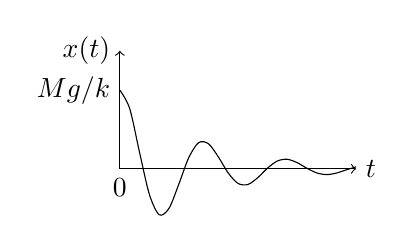
\begin{tikzpicture}
      \draw[->] (0,0) -- (3,0) node[right] {$t$};
      \draw[->] (0,0) -- (0,1.5) node[left] {$x(t)$};
      \draw[domain=0:3,smooth,variable=\x,black] plot ({\x},{exp(-\x)*(cos(6*\x*180/pi)+0.2*sin(6*\x*180/pi)});
      \draw (0,0) node[below]{0};
\draw (0,1) node[left]{$Mg/k$};
\end{tikzpicture}
\end{center}
\item We want the solution to be critically damped, and hence $b=\sqrt{4mk}=\sqrt{4(1267)(4\times10^4)}=1.42\times10^4$ N s/m.
\end{enumerate}
\end{ans}
\begin{qns}[Dispersion]\leavevmode
\begin{enumerate}[label=(\roman*)]
\item Explain what is meant by group velocity, and show that it is given by $v_g=\frac{d\omega}{dk}$.\hfill\textbf{[6]}
\item Show that for a dispersive medium where the phase velocity $v_p$ depends on wavelength, $\lambda$,\hfill\textbf{[4]}
$$v_g=v_p-\lambda\frac{dv_p}{d\lambda}$$
\item When light is refracted at an interface between two media, the angle of incidence, $\theta_1$, and the angle of propagation of the refracted light, $\theta_2$, are related by\hfill\textbf{[6]}
$$v_2\sin\theta_1=v_1\sin\theta_2$$
where $v_1$ and $v_2$ represent the phase velocities of the light in the first and second media, respectively. Light of wavelength $\lambda$ is incident from a vacuum onto an interface with a medium where the speed of light is $v_p(\lambda)$. The angle of incidence is 45.00\degree. For $\lambda=500$ nm, $\theta_2=17.80$\degree. When the wavelength is changed to 498 nm, $\theta_2$ decreases by 0.010\degree, and when the wavelength is changed to 502 nm, $\theta_2$ increases by 0.010\degree. Find the group velocity in the medium at a wavelength of 500 nm.
\item A short pulse of light contains wavelengths centred around 500 nm. Find how long it would take for the pulse to propagate through 1 cm of the medium, and describe qualitatively but in detail what would happen to the pulse as it propagates. \hfill\textbf{[4]}
\end{enumerate}
\end{qns}
\begin{ans}\leavevmode
\begin{enumerate}[label=(\roman*)]
\item The group velocity of a wave is the velocity with which the overall envelope shape of the wave's amplitudes—known as the modulation or envelope of the wave—propagates through space. $v_g=\frac{\partial\omega(k)}{\partial k}$ The wave crests will move relative to the envelope.\\[5pt]
Consider a wavepacket consisting of a carrier wave with wavenumber $k_0$, multiplied by an envelope $f(x)$, such that it has significant amplitude only over a small wavenumber range $\Delta k$, where $\Delta k<<k_0$. Writing $\psi(x,0)$ as $\text{Re}[(\int_{-\infty}^\infty F(k_1)e^{ik_1x}dk_1)e^{ik_0x}]$ such that each sinusoid with wavenumber $k_0+k_1$ will propagate at its own phase velocity and that $F(k_1)$ is the Fourier transform of $f(x)$. At $t>0$, we have
$$\psi(x,t)=\text{Re}\bigg[\int_{-\infty}^\infty F(k_1)e^{i(k_0+k_1)x-(\omega_0+\omega_1)t}dk_1\bigg]$$
where $\omega_0=\omega(k_0)$ and $\omega_0+\omega_1=\omega(k_0+k_1)$. Given the assumption where $F(k_1)$ is non-zero over a small wavenumber range $\pm\Delta k$, where $\Delta k<<k_0$. Expanding $\omega$ about $k_0$,
$$\omega\approx\omega_0+\frac{\partial\omega}{\partial k}\bigg|_{k=k_0}k_1+\frac{1}{2}\frac{\partial^2\omega}{\partial k^2}\bigg|_{k=k_0}k_1^2$$
where $v_g=\frac{\partial\omega}{\partial k}(k=k_0)$ and $v_p=\omega_0/k_0$. Finally,
$$\psi(x,t)=\text{Re}\bigg[\int_{-\infty}^\infty F(k_1)e^{-ik_1v_gt}e^{ik_1x}dk_1e^{i(k_0x-\omega_0t)}\bigg]=\text{Re}[f(x)*\delta(x-v_gt)e^{i(k_0x-\omega_0t)}]$$
and then as desired. Essentially, the modulating envelope propagates at speed $v_g$.
\item With $k=\frac{2\pi}{\lambda}$,
$$v_g=\frac{d\omega}{d k}=\frac{d}{dk}(kv_p)=v_p+k\frac{dv_p}{dk}=v_p-\lambda\frac{dv_p}{d\lambda}$$
\item We have $v_2=\frac{\sin\theta_2}{\sin\theta_1}v_1$ such that $\theta_1=45$\degree. For $\lambda=500$ nm, $\theta_2=17.8$\degree; for $\lambda=498$ nm, $\theta_2=17.79$\degree; for $\lambda=502$ nm, $\theta_2=17.81$\degree. We have
$$\frac{dv_p}{d\lambda}=\frac{c}{\sin(45\degree)}\frac{\sin(17.81\degree)-\sin(17.79\degree)}{4\times10^{-9}}=3.53\times10^{13}$$
$v_p$ is taken to be the averaged at $\lambda=500$ nm, such that $v_p=\frac{c}{\sin(45\degree)}\sin(17.8\degree)=1.297\times10^8$. By the relation in (ii),
$$v_g=v_p-\lambda\frac{dv_p}{d\lambda}=1.297\times10^8-500\times10^{-9}(3.53\times10^{13})=1.12\times10^8m/s$$
\item The time taken for it to travel is $\frac{10^{-2}}{1.12\times10^8}=8.92\times10^{-11}$ s. The pulse will spread out with the variance growing roughly quadratically with time. The initial spatial extent will be large since the pulse is short. As longer wavelengths travel slower, the waves will `pile up' at the front of the wavepacket, exhibiting positive `chirp'.
\end{enumerate}
\end{ans}
\begin{qns}[Fraunhofer Diffraction]\leavevmode
\begin{enumerate}[label=(\roman*)]
\item State the convolution theorem for Fourier transforms, and show with the aid of diagrams how it can be used to predict the Fraunhofer diffraction pattern of a grating
with a finite number of very narrow slits.\hfill\textbf{[6]}
\item A diffraction grating with 500 slits per mm is illuminated at normal incidence with parallel light of wavelength 400 nm. Find the angle of diffraction of the second-order diffraction peak.

\hfill\textbf{[2]}
\item Working with the second-order diffraction peaks, how wide must the grating be in order to resolve two spectral lines close to 400 nm but separated in wavelength by 0.2 nm?\hfill\textbf{[3]}
\item The diffracted light is collected by a lens of focal length 0.25 m. An array detector with a pixel width $t$ is placed at the focus and used to measure the diffraction pattern. What value of $t$ is required to resolve the two spectral lines?\hfill\textbf{[4]}
\item The width of each slit in the diffraction grating used in the experiment above is 1 $\mu$m. Explain why this width of slits causes a problem in the experiment.\hfill\textbf{[5]}
\end{enumerate}
\end{qns}
\begin{ans}\leavevmode
\begin{enumerate}[label=(\roman*)]
\item If $h(x)$ is the convolution of two functions $f(x)$ and $g(x)$, i.e.
$$h(x)=\int_{-\infty}^\infty f(y)g(x-y)dy$$
then their Fourier transforms are related by $\tilde{h}(k)=\tilde{f}(k)\tilde{g}(k)$. For a single narrow slit at $x_0$, it is represented by a delta function $\delta(x-x_0)$. The Dirac comb is thus $f(x)=\sum_{n=-\infty}^\infty\delta(x-na)$ which is an infinite array of slits, each separated by a distance $a$. To select a finite number of these, we multiply by a top-hat function $g(x)$ of width $w$, i.e. $g(x)=1$ for $|x|<w/2$ and $g(x)=0$ for $|x|\geq w/2$.\\[5pt]
The Fraunhofer diffraction pattern caused by light with a wavevector $\mathbf{k}$ normally incident on a grating with aperture function $h(x)$, viewed at an angle $\theta$ from the normal to the grating is described by the complex amplitude, which is directly proportional to
$$\tilde{h}(q)=\int_{-\infty}^\infty h(x)e^{i(kR\sin\theta-\omega t)}dx$$
with $q=k\sin\theta$. For the grating, $\tilde{h}(q)=\tilde{f}(q)*\tilde{g}(q)$ with $\tilde{f}(q)=\sum_{n=-\infty}^\infty\delta(q-\frac{2n\pi}{a})$ and $\tilde{g}(q)=w\sinc(qw/2)$ such that the diffracted intensity is 
$$\propto\bigg|w\sinc(qw/2)*\sum_{n=-\infty}^\infty\delta(q-\frac{2n\pi}{a})\bigg|^2$$
Principal maxima are separated by $k\sin\theta=\frac{2\pi}{a}$, while the first zero of the central maximum has width $\frac{4\pi}{w}$.
\item Second-order peak will be when $q=\frac{2\pi}{d}2$ with $\frac{1}{d}=500$ mm$^{-1}$, corresponding to an angle of
$$\frac{4\pi}{d}q=k\sin\theta\implies\frac{2\lambda}{d}=\sin\theta=\frac{2}{5}\implies\theta=23.6\degree$$
\item By Rayleigh's criterion, the principal maximum of a peak must lie on the next zero of the other. The second order peak is at $\theta=\sin^{-1}(2\lambda/d)$. The next zero is at $\theta+\delta\theta=\sin^{-1}(\frac{2(\lambda+\Delta\lambda)}{d}+\frac{\lambda}{w})$. For the limit of resolvability, we require
$$\sin^{-1}\frac{2\lambda}{d}=\sin^{-1}\bigg(\frac{2(\lambda+\Delta\lambda)}{d}+\frac{\lambda}{w}\bigg)\implies w=\frac{\lambda d}{2\Delta\lambda}=\frac{400\times10^{-9}\times\frac{1}{500}}{2(0.2\times10^{-9})}=2 mm$$
\item At a distance of $f=0.25$ mm, the spectral lines will have a spatial separation of
$$\delta x=f\tan\bigg[\sin^{-1}\bigg(\frac{2(\lambda+\Delta\lambda)}{d}\bigg)\bigg]-f\tan\bigg[\sin^{-1}\bigg(\frac{2\lambda}{d}\bigg)\bigg]=6.5\times10^{-5} m$$
The pixel must have $t<\delta x$ in order to not average over the signal.
\item If the slits are of finite width $\ell$, the aperture function is convolved with a top-hat of width $\ell$, which therefore multiplies the diffracted amplitude by a sinc function. This function has zeroes when $0.5q\ell=n\pi$, with $n\neq 0$, giving rise to missing orders ($n$th order) such that these zeroes lie on the $n$th order peaks.
\end{enumerate}
\end{ans}
\begin{qns}[Thin Film Interference]\leavevmode
\begin{enumerate}[label=(\roman*)]
\item A thin, uniform, transparent film of refractive index $n$ and thickness $d$ is deposited on a flat substrate of refractive index $n_2 > n$. A laser beam of wavelength $\lambda$ is incident from the surrounding air onto the film, at an angle $\theta_i$ from the normal. Show that the phase difference between light reflected at the air-film interface and light passing into the film and being reflected at the film-substrate interface is given by
$$\delta=\frac{4\pi nd}{\lambda}\cos\theta$$
where $\theta$ is the angle of propagation inside the film, given by $n\sin\theta=\sin\theta_i$.\hfill\textbf{[5]}
\item Light of wavelength $\lambda$ and amplitude $A$ is incident on the top surface of the film. A reflection of amplitude $0.15A$ occurs at the top interface (air-film). The wave propagating into the film is partially reflected at the bottom interface (film-substrate) and emerges from the top surface of the film with amplitude $0.03A$. Neglecting any dependence of the reflection and transmission coefficients on wavelength or angle, and assuming that there is no reflection of light leaving the film at the film-air interface, find an expression for the reflected intensity as a function of $\delta$, and sketch it.\hfill\textbf{[5]}
\item In a real experiment, the film refractive index is 1.2 and the wavelength is 500 nm. For angles $\theta_i$ close to 10\degree, bright fringes in the reflected intensity occur at a spacing of 0.4\degree. Find the film thickness, $d$.\hfill\textbf{[6]}
\item Describe qualitatively and explain the behaviour seen when monochromatic light is reflected at normal incidence from an oil film of non-uniform thickness on the surface of a puddle. \hfill\textbf{[4]}
\end{enumerate}
\end{qns}
\newpage
\begin{ans}\leavevmode
\begin{enumerate}[label=(\roman*)]
\item Using Snell's law ($\sin\theta_i=n\sin\theta$), the phase difference $\delta$ is
$$\delta=|k_{air}AD-k_nABC|=\bigg|k_{air}2d\tan\theta\sin\theta_i-nk_{air}\frac{2d}{\cos\theta}\bigg|=n2d\cos\theta\frac{2\pi}{\lambda}$$
\begin{figure}[H]
    \centering
    \includegraphics[scale=0.4]{thinfilm.PNG}
    \caption{Diagram for Thin Film Interference}
\end{figure}
\item Given $r=0.15$ (top surface) and $rr'=0.03$ such that $r'=0.2$ (bottom surface). The interference involves superposing $Are^{i\omega t}$ and $Arr'e^{i(\omega t-\delta)}$ where $A$ is some constant. The superposed intensity is
$$I=[\text{Re}[\psi_1+\psi_2]]^2=\frac{1}{4}(\psi_1+\psi_1^*+\psi_2+\psi_2^*)^2=\frac{1}{4}[2|\psi_1|^2+2|\psi_2|^2+4\text{Re}[\psi_1\psi_2^*]+\psi_1^2+\psi_2^2+(\psi_1^*)^2+(\psi_2^*)^2]$$
the last four terms depends on time. Taking the time-averaged thus gives (shifted cosine graph)
$$\langle I\rangle=\frac{1}{4}[2A^2r^2+2A^2r^2r'^2+4\text{Re}[A^2r^2r'\cos\delta]]=A^2(0.0117+0.00225\cos\delta)$$
\item We have $n=1.2$ and $\lambda=500$ nm. Between two adjacent maxima, $\theta_i$ changes from 10\degree to 10.4\degree. By Snell's Law, $\sin\theta_i=n\sin\theta\implies\cos\theta=\sqrt{1-(\sin\theta_i/n)^2}$. Hence, the change is
$$2\pi=\Delta\delta=\frac{4\pi nd}{\lambda}\Delta\cos\theta=\frac{4\pi nd}{\lambda}[\sqrt{1-(\sin10\degree/n)^2}-\sqrt{1-(\sin10.4\degree/n)^2}]\implies d=2.44\times10^{-4}m$$
\item With normal incidence, but non-parallel sides, there is a phase difference induced by the differing path lengths within the oil. For a fixed incident angle, there will therefore be a variation in space in the interference pattern with different wavelengths obtaining resonance with the film cavity at different thicknesses. Repeating rainbows will be observed tracking the variation in depth of the oil. Restricting to monochromatic light, we will see fringes corresponding to contour lines of constant depth, spaced at $\frac{\lambda_{air}}{2n}$.
\end{enumerate}
\end{ans}
\newpage
\subsubsection{Section C}
\begin{qns}[Phonons]\leavevmode
\begin{enumerate}[label=(\roman*)]
\item Give a brief physical description of a phonon.\hfill\textbf{[2]}
\item Consider a one-dimensional chain of particles where the particles alternate between type A and type B, which have different masses. If the spring constant joining the masses is $\alpha$, show that the angular frequency $\omega$ of small amplitude oscillations along the length of the chain is given by 
\begin{equation}
\omega^2=\frac{\alpha}{m_Am_B}\bigg\{(m_A+m_B)\pm\bigg[(m_A+m_B)^2-4m_Am_B\sin^2(qa)\bigg]^{1/2}\bigg\}\tag{*}
\end{equation}
where $m_A$ and $m_B$ are the masses of the two types of particles, $q$ is the wavevector and $a$ is the spacing between adjacent particles in the chain.\hfill\textbf{[6]}
\item Comment briefly on the physical meaning of the two solutions in equation (*).\hfill\textbf{[2]}
\item In the limit where the wavevector is small, show that the angular frequencies in equation (*) can be described by \hfill\textbf{[4]}
$$\omega\approx\sqrt{\frac{2\alpha(m_A+m_B)}{m_Am_B}},\quad \sqrt{\frac{2\alpha a^2q^2}{m_A+m_B}}$$
The figure below shows the dispersion relationship for phonons travelling in the [111] direction in NaCl, which approximates well to the one-dimensional model considered above as it has alternating planes of Na and Cl atoms.
\begin{figure}[H]
    \centering
    \includegraphics[scale=0.85]{2017P2C10Q.PNG}
\end{figure}
\item Using the small-wavevector limit and the figure, estimate the value for $\alpha$ in this system. [The relative atomic masses of sodium and chlorine can be taken as 23 and 35.5 respectively.]\hfill\textbf{[3]}
\item Using the data in the figure, find a value for the speed of sound in the [111] direction in NaCl and then use this to find the spacing between a plane of Na atoms and the neighbouring plane of Cl atoms.\hfill\textbf{[3]}
\end{enumerate}
\end{qns}
\begin{ans}\leavevmode
\begin{enumerate}[label=(\roman*)]
\item A phonon is a collective harmonic excitation of the atoms with a well-defined frequency, and a fixed relative phase and amplitude between all of the atoms.
\item Let the displacements of the $n$th atoms of type A and B be $u_n$ and $v_n$ respectively, then the equations of motion are
$$m_A\ddot{u}_n=-\alpha(u_n-v_n)-\alpha(u_n-v_{n+1})$$
$$m_B\ddot{v}_n=-\alpha(v_n-u_n)-\alpha(v_n-u_{n-1})$$
Look for solutions of the form $u_n=u_0e^{i(\omega t-2nqa)}$, $v_n=v_0e^{i(\omega t-2nqa)}$ for some complex constants $u_0$ and $v_0$, then we obtain a system of linear equations
$$\begin{pmatrix}\omega^2m_A-2\alpha&\alpha(1+e^{2iq\alpha})\\\alpha(1+e^{-2iq\alpha})&\omega^2m_B-2\alpha\\\end{pmatrix}\begin{pmatrix}u_0\\v_0\\\end{pmatrix}=0$$
The characteristc equation is
$$0=(\omega^2m_A-2\alpha)(\omega^2m_B-2\alpha)-\alpha^2(1+e^{-2iqa})(1+e^{2iaq})=\omega^4m_Am_B-2\alpha\omega^2(m_A+m_B)+\alpha^2(2-2\cos2aq)$$
$$\implies\omega^2=\frac{\alpha}{m_Am_B}[(m_A+m_B)\pm\sqrt{(m_A+m_B)^2-4m_Am_B\sin^2qa}]$$
\item The negative root corresponds to the acoustic mode while the positve root corresponds to the optical mode. At the centre of the Brillouin zone, the neighbouring atoms move in phase and move out of phase by $\frac{\pi}{2}$ radians respectively.
\item When the wavevector is small, $qa<<1$,
$$\omega^2\approx\frac{\alpha(m_A+m_B)}{m_Am_B}\bigg[1\pm\bigg(1-\frac{2m_Am_Bq^2a^2}{(m_A+m_B)^2}+\dots\bigg)\bigg]=\left\{
        \begin{array}{l}
      \frac{2\alpha}{m_Am_B}(m_A+m_B)   \\
      \frac{2\alpha q^2a^2}{m_A+m_B}
        \end{array}
    \right.$$
\item In the small wavevector limit, $\omega_o=4.8\times10^{13}$ rad s$^{-1}$ from the graph and so 
$$\omega_o=\sqrt{\frac{2\alpha(m_A+m_B)}{m_Am_B}}\implies\alpha=\frac{(4.8\times10^{13})^2}{2}\frac{23\times 35.5}{(23+35.5)}(1.6\times10^{-27})=26.7 N/m$$
\item From the graph, the gradient of the acoustic branch (speed of sound) in the low wavevector limit is
$$\frac{\partial\omega_a}{\partial q}=\frac{0.9\times10^{13}}{2\times10^9}=4500 m/s$$
The analytical result is
$$\frac{\partial\omega_a}{\partial q}=\sqrt{\frac{2\alpha}{m_A+m_B}}a\implies a=\sqrt{\frac{m_A+m_B}{2\alpha}}\frac{\partial\omega_a}{\partial q}=\sqrt{\frac{(23+35.5)(1.66\times10^{-27})}{2(26.7)}}4500=1.92\times10^{-10}m$$
which is a reasonable value for lattice spacing.
\end{enumerate}
\end{ans}
\newpage
\begin{qns}[Band Structure]\leavevmode
\begin{enumerate}[label=(\roman*)]
\item Explain, without mathematical details, what is meant by a semiconductor and what differentiates it from a metal. Explain the difference between direct and indirect band gaps and hence describe why it might be easier to make a light-emitting diode from gallium arsenide rather than silicon.\hfill\textbf{[5]}
\item Again without mathematical details explain the concept of doping in semiconductors, including the difference between $p$ and $n$ type. Sketch the energy level structure of a $p$-$n$ junction.

\hfill\textbf{[5]}
\item If the electrons in germanium have an effective mass $m_e^*=0.1$ $m_e$ and a dielectric constant of $\epsilon=16$, then by modifying the Bohr model for hydrogen, determine the energy required to ionise donor states in the material, and the effective radius of the donor states. At 300 K, explain whether it is likely that a significant proportion of the donor atoms will be ionised.

\hfill\textbf{[3]}
\item A germanium [density 5.3 g cm$^{-3}$ relative atomic mass 73] sample is doped by replacing one in every million atoms with single-electron donors. Assuming all of the donors are ionised calculate the ratio of conductivity of the doped sample to the undoped case at 300 K where there are $\approx3\times10^{19}$ conduction electrons per m$^3$.\hfill\textbf{[2]}
\item Describe how the carrier concentration could be measured.\hfill\textbf{[3]}
\item Estimate the doping concentration at which the orbits of the donor states start to overlap.

\hfill\textbf{[2]}
\end{enumerate}
\begin{mdframed}
\color{darkblue}{The Bohr equations for the energies and radii of electron states in a Hydrogen atom are
$$E_n=\frac{m_ee^4}{2\hbar^2n^2(4\pi\epsilon_0)^2}$$
$$r_n=\frac{4\pi\epsilon_0n^2\hbar^2}{m_ee^2}$$
}
\end{mdframed}
\end{qns}
\begin{ans}\leavevmode
\begin{enumerate}[label=(\roman*)]
\item We consider the Nearly Free Electron (NFE) model. The atomic nuclei combined with core electrons give rise to a periodic potential with which the delocalized electrons interact. This periodicity gives rise to a bandstructure and delocalized energy levels which are only meaningful (due to Nyquist) in the first Brillouin Zone. As electrons are spin-half particles, each energy state can be occupied by two electrons, and there are exactly enough states within each band in the first Brillouin Zone for two electrons per real space lattice point.\\[5pt]
At $T=0$ K, electrons fill up states in order of increasing energy. If there is a finite energy gap between the last occupied state and the next unoccupied state, then the material will be an insulator. Otherwise, it is a metal where an arbitrarily small external electric field can excite the electrons into nearby unoccupied states. At $T\neq 0$ K, when the bandgap $E_g\sim k_BT$, a number of electrons may jump from valence band to conduction band, which has many accessible states. The material will therefore conduct, but to a lesser extent than a metal due to the exponentially decaying factor $e^{-E_g/k_BT}$ in the number of charged carriers.\\[5pt]
When an electron in an excited state decays to a lower unoccupied state, it needs in general to change its momentum, as well as, emitting the energy. For direct bandgap structures, there is negligible momentum change, whereas for indirect bandgap structures, a non-trivial momentum change is necessary. The momentum of a phonon per unit energy is too small to carry away all the energy and all the momentum, so a phonon must also participate in the transition. For a light-emitting diode, the former is preferred since the additional phonon dissipates energy away its heat, resulting in fewer electrons being able to participate in this energy level transition, hence effectively reduced power.
\item Adding dopants that gives more (fewer) electrons than the substrate itself creates an n-type (a p-type) semiconductor. At non-zero temperatures, all these states are ionized, increasing the conductance of the material. For the n-type (p-type), the vast majority of the charge carriers are ionized electrons (holes left behind when electrons from the filled band were excited into the dopant hole state). In the absence of impurities, the Fermi energy ($\mu(T=0)$) is in the middle of the band gap. When the donor (acceptor) impurities are added, at zero temperature, impurity states near the top (bottom) of the bandgap are filled (empty). The Fermi energy is moved up to the top (down to the bottom) of the band gap.\\[5pt]
When an n-type semiconductor is placed next to a p-type semiconductor, the differences in chemical potentials causes charge to flow until an electric dipole is formed at the surface, creating a contact potential to prevent any further net flow of charge.
\item The effective radius of the donor state is
$$r_1=\frac{4\pi\epsilon_r\epsilon_0\hbar^2}{m^*e^2}=\frac{4\pi(16)(8.85\times10^{-12})(6.626\times10^{-34}/2\pi)^2}{0.1(9.11\times10^{-31})(1.6\times10^{-19})^2}=8.49 nm$$
The energy required to ionize donor states is
$$E=\frac{0.1}{16^2}13.6=5.3meV$$
which is less than $k_BT=26$ meV, and all the donor states will be ionized.
\item The number density of dopants is
$$n=\frac{1}{10^6}\frac{\rho_{Ge}}{m_{Ge}}=\frac{5300}{10^6\times 73\times 1.66\times10^{-27}}=4.35\times10^{22}m^{-3}$$
and assuming all the dopants ionized, the resulting conductance is
$$\sigma=\frac{nq^2\tau}{m^*}$$
where $m^*=0.1m_e$. The ratio of conductivity is the ratio of number densities and is $4.35\times10^{22}/3\times10^{11}=1450$.
\item The carrier concentration can be measured by using Hall effect. Apply a steady current through a long thin bar with magnetic field $\mathbf{B}$ perpendicular to current density $\mathbf{J}$. The Hall coefficient is defined as
$$R_H:=\frac{\mathbf{E}}{\mathbf{B}\times\mathbf{J}}$$
In steady state, the net force is zero with
$$\boldsymbol{0}=\mathbf{F}=q(\mathbf{E}+\mathbf{v}\times\mathbf{B})\implies v=\frac{J}{nq},~R_H=\frac{1}{nq}$$
We can measure both $\mathbf{B}$, $\mathbf{E}$ and $\mathbf{J}$ and by assuming the charge of each carrier is $e=1.6\times10^{-19}$C, then we can deduce carrier concentration.
\item The donor states will not overlap as long as the radius of the Hydrogenic donor orbits is small compared to the inter-dopant spacing $1/n^{1/3}$, so 
$$n_{crit}=r^{-3}=1.6\times10^{-24}m^{-3}$$


\end{enumerate}
\end{ans}
\newpage
\subsubsection{Section D}
\begin{qns}[OWO Essay]
Write an essay on diffraction patterns of simple circular holes and obstructions, in both the Fraunhofer and Fresnel regimes.\hfill\textbf{[20]}
\end{qns}
\begin{ans}
Consider a spherical source with strength $a_S$, at distance $s(x,y)$ from the aperture element $dxdy$ (with overall aperture function $h(x,y)$, then the total amplitude at point P, at a distance $r$ from the aperture element, is
$$\psi_P=-\int\frac{i}{\lambda}h(x,y)K(\theta)\frac{a_Se^{ik(s+r)}}{sr}dxdy$$
where $K(\theta)$ is the obliquity factor. This is the Fresnel-Kirchhoff diffraction integral, which is valid in the limit of distances greater than the wavelength of light, allowing us to neglect the vector nature of the electromagnetic wave.\\[5pt]
In the case of Fraunhofer diffraction (diffracted beam close to the axis), we assume P close to the axis such that $K=1$ and $x_0/L<<1$, $y_0/L<<1$ and that $R$ is large, then the distance $r$ from the aperture element $dxdy$ to P is
$$r^2\approx L^2+(x_0-x)^2+(y_0-y)^2\approx R^2\bigg(1-2\frac{x_0x+y_0y}{R^2}\bigg)$$
where $R^2=L^2+x_0^2+y_0^2$. Using binomial expansion, we obtain $r\approx R-\frac{x_0x+y_0y}{R}$. Equivalently, for an aperture of maximum extent $D$, is $R>>D^2/\lambda$. So the Fraunhofer integral is essentially a Fourier transform of the aperture function, i.e.
$$\int_\Sigma\psi_\Sigma h(x,y)e^{-ik(x_0x+y_0y)/R}dxdy\propto\mathcal{F}[h(x,y)]$$
The aperture function of a circular aperture is $h(\rho)=1$ for $\rho<0.5D$ where $D$ is the aperture diameter, and zero otherwise. 
Changing to plane polar coordinates, we have the diffraction amplitude to be directly proportional to
$$\int_0^{2\pi}\int_0^{D/2}e^{-ik_x\rho\cos\phi}\rho d\rho d\phi$$
where we set the wavevector to be along the $x$ direction without loss of generality (due to circular symmetry). Now using the identity $\int_0^{2\pi}e^{-ik_x\rho\cos\phi}d\phi=2\pi J_0(k_x\rho)$ and $\int_0^{k_xD/2}J_0(k_x\rho)k_x\rho d(k_x\rho)=0.5k_xDJ_1(k_xD)$, where $J_1$ and $J_0$ are the first and zero order Bessel function of the first kind respectively, then 
$$2\pi\int_0^{D/2}J_0(k_x\rho)\rho d\rho=2\pi\frac{1}{k_x^2}J_0\int_0^{k_xD/2}J_0(k_x\rho)k_x\rho d(k_x\rho)=\frac{2\pi}{k_x^2}k_x\frac{D}{2}J_1(k_xD/2)$$
The intensity can be written to be directly proportional to 
$$\bigg(\frac{J_1(\pi\sin\theta D/\lambda)}{\pi D\sin\theta/\lambda}\bigg)^2$$
$J_1(\chi)$ has first zero at $\chi\approx3.83$ so the diffracted intensity has a zero at $\sin\theta\approx1.22\lambda/D$. The region inside this first zero is the Airy disc, and it contains 86 percent of the total energy flux. Below is a sketch of the diffraction intensity as a function of $\frac{\pi\sin\theta D}{\lambda}$.
\begin{center}
  \begin{tikzpicture}
    \begin{axis}[width=\textwidth, height=0.5*\textwidth,
    xlabel=$\pi D\sin\theta/\lambda$, ylabel=$|J_1(\pi D\sin\theta/\lambda)/(\pi D\sin\theta/\lambda)|^2$,yticklabels={,,}]
    \addplot+[id=parable,domain=-10:10, samples=300, mark=none, width=2pt, color=black]
    gnuplot{(besj1(x)/x)^2}{};
   \end{axis}
  \end{tikzpicture}
\end{center}
In the case of Fresnel diffraction (diffracted beam on-axis), we assume further that
\begin{itemize}
    \item the angles to the edge of the aperture are small enough that we can neglect the obliquity factor, and thus take $K(\theta)=1$;
    \item that the variations in $r_1$ and $r_2$ over the aperture are negligible as far as the denominator is concerned: $r_1\sim a$ and $r_2\sim b$ but note variations in $(r_1+r_2-a-b)$ are not negligible compared with $\lambda$ and so have a significant effect on the phase term.
\end{itemize}
Under these approximations, we have $\psi_P(0,0)$ to be directly proportional to
$$\int_\Sigma h(x,y)e^{ik(x^2+y^2)/2R}dxdy$$
where the path from S to P via the aperture element at $(x,y)$ is
$$r_1+r_2\approx a+b+\frac{x^2+y^2}{2a}+\frac{x^2+y^2}{2b}$$
Writing $\frac{1}{R}=\frac{1}{a}+\frac{1}{b}$, we have the optical path to be directly proportional to $(x^2+y^2)/2R$. Here, the quadratic phase in the diffraction integral can't be ignored since the distances between the screen and the aperture is of order $D^2/\lambda$ or smaller, where $D$ is the maximum dimension of the aperture.\\[5pt]
Consider a circular aperture of radius $r_a$. The obliquity factor, as well as, the variation in $r_1$ and $r_2$ across the aperture are retained. We only consider the pattern on-axis. Dividing the aperture elements of radius $\rho$ and thickness $d\rho$, we have the diffraction integral to be
$$\int_{\rho=0}^{\rho=r_a}\frac{K}{(a^2+\rho^2)^{0.5}(b^2+\rho^2)^{0.5}}e^{0.5ik\rho^2/R}2\pi\rho d\rho=\int_{s=0}^{s=r_a^2}\frac{K(s)}{(a^2+s)^{0.5}(b^2+s)^{0.5}}e^{i\pi s/(\lambda R)}\pi ds$$
The integral can be evaluated graphically using the phasor diagram. The phase $\phi=\frac{\pi s}{\lambda R}$ varies linearly with $s$, and the elemental contributions to the integral are approximately $ds$, so as $s$ increases the phasor diagram is approximately a circle. The term before the exponential is a slowly decreasing function of $s$ (denominator obviously increases with $s$, and $K$ decreases with $s$), thus the radius of the circle in the phasor diagram gradually decreases with $s$. To calculate the diffracted amplitude, consider the spanning vector from point O to the point a distance $s$ along the curve. The curve spirals inwards, so in the absence of an obstruction or aperture, the integration range is from O to F, corresponding to $s=\infty$. OF is thus the amplitude of the unobstructed wavefront.
\begin{figure}[H]
    \centering
    \includegraphics[width=\linewidth]{fresnelcircular.PNG}
    \caption{Left: Fresnel Diagram for Circular aperture. Top Right: Fresnel half period zones. Bottom Right: Phasor Diagram for a central obstacle.}
\end{figure}
In the circular geometry, these are concentric circular zones in the aperture plane, over which the phase at the observation point changes by $\pi$. We define the first zone as the circular region in the aperture plane which satisfies $0\leq\phi(\rho)\leq\pi$, which corresponds to $\rho^2\leq\lambda R$. The $n$th zone corresponds to the annulus satisfying $(n-1)\pi\leq\phi(\rho)\leq n\pi\implies\sqrt{(n-1)\lambda R}\leq\rho\leq\sqrt{n\lambda R}$. Note that the area of each zone is the same, in the quadratic approximation:
$$\pi(\rho_n^2-\rho_{n-1}^2)=\pi\lambda R$$
If we neglect the obliquity factor and the variation of $r_1$ and $r_2$, each zone would contribute equally to the amplitude at P. The phasor diagram would be circular. Odd numbered zones add to, and even numbered zones subtract from the overall amplitude at P. So on the optic axis of a circular aperture of radius $r_a$, the aperture includes $N$ zones, given by $r_a^2=N\lambda R$.\\[5pt]
If $N$ is odd, we get a bright spot at P, $\psi\sim2\psi_u$ (unobstructed). If $N$ is even, we get a dark spot at P, hence $\psi\sim 0$. For large apertures, the small angle approximations begin to break down. The spiralling in effect in the phasor diagram due to the $1/r$ terms in the diffraction integral becomes noticeable. This effect is further enhanced since $K(s)<1$. The width of the outer zones also increases, as the higher-order terms become important.\\[5pt]
Consider a circular obstruction on the axis. For an obstacle of radius $r_a$, the inner zones up to $\rho=r_a$ are obscured, but all the outer zones are clear. The limits of integration for the diffraction integral are $\rho=r_a$ to $\rho=\infty$. The relevant spanning vector in the phasor diagram is from F to A, which spans an arc angle of $\phi_a=\frac{\pi r_a^2}{\lambda R}$.\\[5pt]
Provided that $r_a$ is not too large, the intensity is therefore close to that expected in the absence of any obstruction. This leads to a bright spot on the axis, known as Poisson's spot. Close to the obstruction, the diffracted angles become large so that $K$ falls, and no spot is observable.
\end{ans}
\newpage
\begin{qns}[CMP Short Notes]
Write brief notes on two of the following:\hfill\textbf{[20]}
\begin{itemize}
    \item the Debye theory of heat capacity in solids;
    \item the concept of effective mass in condensed matter physics and its relation to electrical transport properties;
    \item the reciprocal lattice and Brillouin zones.
\end{itemize}
\end{qns}
\begin{ans}\leavevmode
\subsubsection*{The Debye theory of heat capacity in solids:}
In 1819, Dulong and Petit realized the heat capacity per atomic weight of a substance is approximately constant. More specifically, near room temperature, the heat capacity of most solids is roughly $3R$ per mole or equivalently $3k_B$ per atom. This is due to equipartition theorem, where each quadratic contribution to the energy (lattice vibration in each independent direction) gives $k_B$ per atom. At low temperatures, experiments show the heat capacity of insulators usually varies proportionally to $T^3$. To understand this, we explain the Debye model.\\[5pt]
In the Debye model, we assume the lattice vibrations are waves with speed $v_s$, speed of sound in the solid, i.e.for all wavelengths, $\omega=v_sq$, where $q$ is the wavevector of the lattice vibration. We compute the density of states of lattice vibrations in 3D as a function of $q$:\\[5pt]
The allowed states form a regular lattice of points in the positive octant of $k$-space. Each state occupies a volume of $\pi^3/V$. We consider the states within a shell of width $dk$, at radius $k$. The number of states in the shell is the volume of the shell divided by the volume of one state.
$$dN=g(k)dk=\frac{3(4\pi k^2/8)dk}{\pi^3/V}=\implies g(k)=\frac{3Vk^2}{2\pi^2}$$
where we included a factor of 3 to allow for 2 transverse modes and 1 longitudinal mode. Hence,
$$g(q)dq=\frac{4\pi q^2dq}{(2\pi/L)^3}3\implies g(\omega)d\omega=\frac{3V\omega^2d\omega}{2\pi^2v_s^3}$$
such that $\int_0^{\omega_D}g(\omega)d\omega=3N$ where $\omega_D$ the cutoff frequency (Debye frequency) is imposed to have a finite number of modes. We then have $\omega_D^3V=6N\pi^2v_s^3$ and hence rewriting $g(\omega)d\omega=\frac{9N\omega^2d\omega}{\omega_D^3}$. We can thus define a Debye temperature $\Theta_D=\hbar\omega_D/k$. Let $\beta=1/k_BT$, the internal energy is 
$$U=\int_0^{\omega_D}g(\omega)\hbar\omega(0.5+(e^{\beta\hbar\omega}-1)^{-1})d\omega=\frac{9}{8}N\hbar\omega_D+\frac{9N\hbar}{\omega_D^3}\int_0^{\omega_D}\frac{\omega^3d\omega}{e^{\hbar\omega\beta}-1}$$
The heat capacity per mole will be $\frac{9R}{x_D^3}\int_0^{x_D}\frac{x^4e^xdx}{(e^x-1)^2}$ where $x_D=\hbar\omega_D/k_BT$. At high temperature $C\rightarrow\frac{9R}{x_D^3}\int_0^{x_D}\frac{x^4}{x^2}dx=3R$ as expected. At low temperatures, $C\rightarrow\frac{9R}{x_D^3}\int_0^\infty\frac{x^4e^xdx}{(e^x-1)^2}=\frac{12R\pi^4}{5x_D^3}$, hence proportional to $T^3$. This is the phononic contribution to the heat capacity.\\[5pt]
Aluminium is a good representative example. Both the experimental and approximate Debye density of states are similar at low $\omega$ as expected. The largest deviations occur near the zone boundary. In fact, the transverse and longitudinal modes have different dispersion curves. In our theory, the Debye frequency was introduced in an ad-hoc fashioned to keep the total number of modes constant. Moreover, the linear dispersion relation was previously shown to only hold for long wavelength limit, but was assumed to hold for all wavelength here.
\subsubsection*{The concept of effective mass in condensed matter physics and its relation to electrical transport properties:}
The effective mass accounts for the influence of the periodic lattice potential on the electron's motion. With this, we can continue to use semi-classical equations of motion to study electron dynamics in a solid. The `kinetic energy' is a function of $k$ and encapsulates the effective mass.
$$\epsilon(k)=\frac{\hbar^2k^2}{2m^*}\implies m^*=\hbar^2\bigg(\frac{d^2\epsilon}{dk^2}\bigg)^{-1}$$
When discussing electrical transport, we make the following assumptions:
\begin{enumerate}
    \item Independent electron approximation: neglect electron-electron interactions between collisions; Free electron approximation: neglect electron-ion interactions. The electrons respond solely to the externally applied fields.
    \item Collisions are instantaneous events that abruptly alter the velocity of an electron. Drude attributed them to the electrons bouncing off the impenetrable ion cores.
    \item Electron experiences a collision with a probability per unit time $1/\tau$, where $\tau$ is the relaxation time. An electron picked at random at a given moment will, on the average, have been travelling for a time $\tau$ before its next collision, and will, on the average, have been travelling for a time $\tau$ since its last collision. $\tau$ is independent of the electron's position and velocity.
    \item Electrons are assumed to achieve thermal equilibrium with their surroundings only through collisions. Immediately after each collision, an electron is taken to emerge with a velocity that is not related to its velocity just before the collision, but randomly oriented and with a speed appropriate to the temperature prevailing at the place where the collision occurred.
\end{enumerate}
With the application of a DC electric field, the acceleration of the electron is $\frac{-e\mathbf{E}}{m}$. $m$ is usually called the effective mass $m^*$ and is usually different from $m_e$ (rest mass of electron in the absence of a lattice) due to the influence of the lattice. The drift velocity is then defined as
$$\mathbf{v_{drift}}=\frac{-e\mathbf{E}\tau}{m}$$
The average $t$ is the relaxation time $\tau$ and since $\mathbf{J}=-ne\mathbf{v}$, we have $\mathbf{J}=\frac{ne^2\tau}{m}\mathbf{E}$ with DC conductivity
$$\sigma_{DC}=\frac{ne^2\tau}{m}$$
The electron mobility is
$$\mu=\frac{v_{drift}}{E}=\frac{e\tau}{m}$$
At any time $t$, the average electronic velocity is $\mathbf{v}$ is just $\frac{\mathbf{p}(t)}{m}$, where $\mathbf{p}$ is the total momentum per electron. Hence the current density is $\mathbf{J}=-\frac{ne\mathbf{p}(t)}{m}$.\\[5pt]
Given that the momentum per electron is $\mathbf{p}(t)$ at time $t$, an electron taken at random at time $t$ will have a collision before time $t+dt$, with probability $\frac{dt}{\tau}$ and will therefore survive to time $t+dt$ without suffering a collision with probability $1-\frac{dt}{\tau}$. If it experiences no collision, however, it simply evolves under the influence of the force $\textbf{f}(t)$. The contribution of all those electrons that do not collide between $t$ and $t+dt$ to the momentum per electron at time $t+dt$ is the fraction $(1-dt/\tau)$ times their average momentum per electron. The equation of motion is thus
$$\mathbf{p}(t+dt)=(1-dt/\tau)[\mathbf{p}(t)+\mathbf{f}(t)dt]=\mathbf{p}(t)-(dt/\tau)\mathbf{p}(t)+\mathbf{f}(t)\implies\frac{d\mathbf{p}(t)}{dt}=-\frac{\mathbf{p}(t)}{\tau}+\mathbf{f}(t)$$
The total collision rate is the sum of the rates of the individual types of collisions. Hence, the relaxation times add like
$$\frac{1}{\tau}=\sum_i\frac{1}{\tau_i}$$
Consider a time-dependent AC electric field of the form $\mathbf{E}(t)=\text{Re}[\mathbf{E}(\omega)e^{i\omega t}]$. The equation of motion is $\frac{d\mathbf{p}}{dt}=-\frac{\mathbf{p}}{\tau}-e\mathbf{E}$. We seek a steady-state solution of the form $\mathbf{p}(t)=\text{Re}[\mathbf{p}(\omega)e^{i\omega t}]$ and have $\mathbf{J}(t)$ to adopt a similar form, we then have
$$\mathbf{J}(\omega)=\frac{ne^2}{m}\frac{1}{(1/\tau)+i\omega}\mathbf{E}(\omega)$$
We then have the frequency-dependent conductivity
$$\sigma_{AC}(\omega)=\frac{1}{1+i\omega\tau}\frac{ne^2\tau}{m}=\frac{ne^2\tau}{m}\frac{1-i\omega\tau}{1+\omega^2\tau^2}$$
The real part has its point of inflexion at $\omega=1/\tau$, which coincide with the peak of the imaginary part. The most important application is the propagation of electromagnetic radiation in a metal. The accompanied perpendicular magnetic field may be ignored for non-relativistic velocities. Moreover, we require the field to not vary appreciably over distances comparable to the electronic mean free path.
\newpage
\subsubsection*{The reciprocal lattice and Brillouin Zones:}
To understand the reciprocal lattice and Brillouin zones, we first talk about these crystal lattices in real space. A Bravais lattice is an infinite periodic array of discrete points with an arrangement and orientation that appears exactly the same, from whichever of the points the array is viewed. In three dimensions, points of a lattice are indexed by three integers
$$\mathbf{R}_{[n_1,n_2,n_3]}=n_1\mathbf{a_1}+n_2\mathbf{a_2}+n_3\mathbf{a_3},\quad n_1,n_2,n_3\in\mathbb{Z}$$ 
where $\mathbf{a_1},\mathbf{a_2},\mathbf{a_3}$ are primitive lattice vectors and its choice are not unique. It turns out that any periodic structure can be expressed as a lattice of repeating motifs. A Bravais lattice has the property that any point looks like the same in any point. Two Bravais lattices are equivalent if they share the same symmetry.\\[5pt]
For every crystal, we can define a unit cell. A unit cell is a region of space such that when many identical units are stacked together if it completely fills all of space and reconstructs the full structure. A primitive unit cell is a region of space that, when translated by $\mathbf{a_i}$, tessellates the space. In a unit cell, it contains exactly one lattice point. One can proceed to define the Wigner-Seitz cell $\Gamma$ (also known as Voroni cell), which is a canonical primitive unit cell.\\[5pt]
Given a lattice point, the set of all points in space which are closer to that given lattice point than to any other lattice point constitute the Wigner-Seitz cell of the given lattice point. To be specific, pick an origin lattice site in $\Lambda$.
$$\Gamma=\{\mathbf{x}:|\mathbf{x}|<|\mathbf{x}-\mathbf{r}|~\forall\mathbf{r}\in\Lambda\text{ such that }\mathbf{r}\neq\boldsymbol{0}\}$$
i.e. it is the region of space closer to a lattice site than to any other site. More concretely, we perform the following procedure in our construction: Choose a lattice point and draw lines to all of its possible near neighbours (not just its nearest neighbours). Then draw perpendicular bisectors of all of these lines. The perpendicular bisectors bound the Wigner-Seitz cell.\\[5pt]
Wigner-Seitz cell will display the full symmetry of the Bravais lattice, but not necessarily all primitive cells will.  Due to translational symmetry of the Bravais lattice, the Wigner-Seitz cell about any one lattice point must be taken into the Wigner-Seitz cell about any other, when translated through the lattice vector that joins the two points.\\[5pt]
For every Bravais lattice $\Lambda$, the  corresponding reciprocal lattice $\Lambda^*$ (also known as dual lattice) is defined by
$$\Lambda^*=\bigg\{\mathbf{k}=\sum_lm_l\mathbf{b_l},~m_l\in\mathbb{Z}\bigg\}$$
where $\mathbf{a_i}\cdot\mathbf{b_j}=2\pi\delta_{ij}$ which is equivalent to $e^{i\mathbf{k}\cdot\mathbf{r}}=1$ $\forall\mathbf{r}\in\Lambda$ and $\mathbf{k}\in\Lambda^*$. In 3D, we can construct $\mathbf{b_i}$ by $\mathbf{b_i}=\frac{2\pi}{V}\frac{1}{2}\epsilon_{ijk}\mathbf{a_j}\times\mathbf{a_k}$ and conversely $\mathbf{a_i}=\frac{2\pi}{V^*}\frac{1}{2}\epsilon_{ijk}\mathbf{b_j}\times\mathbf{b_k}$ with $V^*=|\mathbf{b_1}\cdot(\mathbf{b_2}\times\mathbf{b_3})|=\frac{(2\pi)^3}{V}$, where $V$ is the volume of the real space lattice. The reciprocal lattice is a Bravais lattice in reciprocal space. Obviously, the reciprocal of the reciprocal lattice is the corresponding real space lattice.\\[5pt]
Finally, a Brillouin zone is any primitive unit cell of the reciprocal lattice. The Wigner-Seitz cell of the reciprocal lattice is the Brillouin Zone. The Brillouin zone is a consequence  of Nyquist's sampling theorem. The translational symmetry of atoms in a solid resulting from the regular lattice spacing, is equivalent to an effective sampling of the atoms of the solid and thus gives rise to the Brillouin zone. For a 1D crystal of lattice constant $a$, the first Brillouin zone is defined as the region where $|\mathbf{k}|<\pi/a$. To elaborate, we discuss two examples of 3D crystals.\\[5pt]
The bcc lattice is a simple cubic lattice where there is an additional lattice point in the very centre of the cube. The Wigner-Seitz cell of BCC is a truncated octahedron with volume $V=a^3/2$ where $a$ is the lattice constant. The hexagonal faces bisect lines joining the central point to points on vertices. The square faces bisect lines joining the central point to other central points in each of the six neighbouring cubic cells.\\[5pt]
The fcc lattice is a simple cubic lattice where there is an additional lattice point in the centre of every face of every cube. The Wigner-Seitz cell of fcc is rhombic dodecahedron with volume $V=a^3/4$. Each of the 12 congruents faces is perpendicular to line joining central point to a point on the centre of the edge.\\[5pt]
The reciprocal of bcc lattice is fcc, i.e. the first Brillouin zone of the bcc is just the fcc Wigner-Seitz cell. Conversely, the first Brillouin zone of the fcc lattice is just the bcc Wigner-Seitz cell.
\end{ans}
\newpage
\section{2018}
\subsection{Paper 1}
\subsubsection{Section A}
\begin{qns}[Identical Particles]
Lithium has an atomic number of 3. Are $^6$Li and $^7$Li atoms bosons or fermions? Explain your reasoning.\hfill\textbf{[4]}
\end{qns}
\begin{ans}
A composite system will be a boson (fermion) if the total spin is an integer (half-integer). Lithium atom has 3 electrons and 3 protons but $^6$Li has odd number of fermions (thus it is a fermion) while $^7$Li has even number of fermions (thus it is a boson).
\end{ans}
\begin{qns}[1D Potential]
An electron is in the ground state of a one-dimensional infinitely deep quantum well. The maximum wavelength at which it can absorb electromagnetic radiation is 800 nm. Calculate the width of the well.\hfill\textbf{[4]}
\end{qns}
\begin{ans}
The maximum wavelength occurs when the electron jumps from the ground state to the first excited state. The width of the well is 0.85 nm
$$\frac{hc}{\lambda}=\Delta E=\frac{\hbar^2}{2m_e}\frac{\pi^2}{L^2}\Delta(n^2)\implies L=\sqrt{\frac{h\lambda}{8m_ec}\Delta(n^2)}=\sqrt{\frac{(6.626\times10^{-34})(800\times10^{-9})(2^2-1^2)}{8(9.11\times10^{-31})(3\times10^8)}}$$
\end{ans}
\begin{qns}[Spin]
The eigenfunctions of the spin-half operator $\hat{S}_z$ are $\alpha$ and $\beta$ with eigenvalues $+\hbar/2$ and $-\hbar/2$ respectively. Find the eigenvalues and eigenfunctions of $\hat{S}_x$.\hfill\textbf{[4]}
\end{qns}
\begin{ans}
Recall the matrix representations of the spin-half operators. Then $\alpha=(1,0)$, $\beta=(0,1)$. Diagonalize $\hat{S}_x$ to find the eigenvalues ($\lambda=\pm0.5\hbar$) and the corresponding normalized eigenvectors $\frac{1}{\sqrt{2}}(1,\pm1)=\frac{1}{\sqrt{2}}(\alpha\pm\beta)$. 
\end{ans}
\begin{qns}[Error Analysis]
The moment of inertia, $I$, of a thin disk is given by $I=\frac{1}{2}\pi\rho sR^4$, where $\rho$ denotes the density of the material, $s$ its thickness and $R$ the radius. A set of disks with $R\approx 1$ m is machined out of a material with $s\approx 0.01$ m and $\rho\approx 8\times10^3$ kg m$^{-3}$ both known to an accuracy of 1\%. Calculate $I$. Determine the accuracy needed in $R$ to ensure that $I$ has an accuracy of 2.5\%.\hfill\textbf{[4]}
\end{qns}
\begin{ans}
$$I=\frac{1}{2}\pi\rho sR^4=\frac{1}{2}\pi(8\times10^3)(0.01)1^4=126 kg m^2$$
The error is
$$\bigg(\frac{\sigma_I}{I}\bigg)^2=\bigg(\frac{\sigma_\rho}{\rho}\bigg)^2+\bigg(\frac{\sigma_s}{s}\bigg)^2+\bigg(4\frac{\sigma_R}{R}\bigg)^2\implies 0.025^2=0.01^2+0.01^2+16\bigg(\frac{\sigma_R}{R}\bigg)^2$$
which gives us $\Delta R=0.00515 R=0.0052$. $R$ needs to be measured within an accuracy of 5.2 mm.
\end{ans}
\begin{qns}[Op-Amp and Filters]
An ideal low-pass filter is designed with an input resistance of 10 $k\Omega$ and time constant of 1 $\mu$s. Sketch the circuit diagram of the filter and determine its capacitance. Sketch the gain as a function of frequency on a Bode plot.\hfill\textbf{[4]}
\end{qns}
\begin{ans}
Low-pass filter has $V_{out}$ across the capacitor of the RC circuit, so
$$\frac{V_{out}}{V_{in}}=\frac{Z_C}{Z_R+Z_C}=\frac{1/i\omega C}{R+(1/i\omega C)}=\frac{1}{1+i\omega RC}$$
Then, $|\frac{V_{out}}{V_{in}}|=1$ as $\omega=0$ and $|\frac{V_{out}}{V_{in}}|\rightarrow0$ as $\omega\rightarrow\infty$. The time constant is $\tau=RC=1\times10^{-6}$ s, but $R=10\times10^3$ $\Omega$. Hence, $C=10^{-11}$ F. The point of inflexion of the graph is at $\omega=\frac{1}{2RC}=0.5\times10^6$ rad/s.
\end{ans}
\newpage
\subsubsection{Section B}
\begin{qns}[1D Potential]
Particles of mass $m$ move in a one-dimensional potential $V(x)$ with a wavefunction $\psi(x,t)$, which satisfies the time-dependent Schrodinger equation.
\begin{enumerate}[label=(\alph*)]
\item Show that the probability current is given by\hfill\textbf{[6]}
$$J(x,t)=\frac{i\hbar}{2m}\bigg(\frac{\partial\psi^*}{\partial x}\psi-\psi^*\frac{\partial\psi}{\partial x}\bigg)$$
\item Particles of mass $m$ and energy $E$ with the wavefunction \hfill\textbf{[5]}
$$\psi(x,t)=Ae^{i(kx-\omega t)}$$
moving in the positive $x$-direction are incident on a double potential step defined by
$$V(x)=
\left\{
        \begin{array}{ll}
      0 & x<0 \\
      V_1 & 0\leq x\leq a\\
      V_2 & x>a
        \end{array}
    \right.$$
where $E > V_2 > V_1 > 0$. Write down the wavefunctions in the three regions. What boundary conditions apply at the potential steps? Explain the physical significance of these boundary conditions.
\item Find the relation between $E$, $V_1$ and $V_2$ that is necessary for zero reflection.\hfill\textbf{[5]}\\[5pt]
You may assume that $\sqrt{2m(E-V_1)/\hbar^2}=\pi/(2a)$.
\item Find an expression relating the amplitude of the transmitted wave to the incident wave and show that the incident and transmitted waves have equal probability current.\hfill\textbf{[4]}
\end{enumerate}
\end{qns}
\begin{ans}\leavevmode
\begin{enumerate}[label=(\alph*)]
\item By the conservation of probability,
$$0=\frac{d}{dt}\int_S|\psi|^2dV+\int_{\partial S}\mathbf{J}\cdot d\mathbf{S}=\int_S\frac{\partial}{\partial t}|\psi|^2+\boldsymbol{\nabla}\cdot\mathbf{J}dV$$
where we used the Divergence Theorem. Since the integration is taken over an arbitrary region, the integrand is true $\forall\mathbf{x},t$. In one-dimension, we have
$$\frac{\partial J}{\partial x}=-\frac{\partial\psi}{\partial t}\psi^*-\psi\frac{\partial\psi^*}{\partial t}=\frac{\hbar}{2mi}\psi^*\frac{\partial^2\psi}{\partial x^2}+\frac{V}{i\hbar}\psi^*\psi-\frac{\hbar}{2mi}\psi\frac{\partial^2\psi^*}{\partial x^2}-\frac{V}{i\hbar}\psi\psi^*=\frac{\hbar}{2mi}\bigg(\psi^*\frac{\partial^2\psi}{\partial x^2}-\psi\frac{\partial^2\psi^*}{\partial x^2}\bigg)$$
Integrating everywhere and realize $\psi\rightarrow0$ for $x\rightarrow\pm\infty$, then the integration constant is zero and we obtain our desired result for $J(x,t)$.
\item We guess our wavefunction to have the asymptotic form
$$\psi(x,t)=
\left\{
        \begin{array}{ll}
      Ae^{i(k_x1-\omega t)}+Are^{-i(k_1x-\omega t)} & x<0 \\
      Be^{i(k_2x-\omega t)}+Ce^{-i(k_2x+\omega t)} & 0\leq x\leq a\\
      D\tau e^{i(k_3(x-a)-\omega t)} & x>a
        \end{array}
    \right.$$
where $k_1=\frac{\sqrt{2mE}}{\hbar}$, $k_2=\frac{\sqrt{2m(E-V_1)}}{\hbar}$, $k_3=\frac{\sqrt{2m(E-V_2)}}{\hbar}$. The boundary conditions are
\begin{itemize}
    \item $\psi$ is continuous everywhere, to give finite momenta everywhere;
    \item $\frac{\partial\psi}{\partial x}$ is continuous everywhere, to give finite accelerations everywhere.
\end{itemize}
\item Zero reflection will require $r=0$, and imposing the boundary conditions:
$$A(1+r)=B+C\implies A=B+C$$
$$Aik_1(1-r)=ik_2(B-C)\implies\frac{k_1}{k_2}A=B-C$$
$$Be^{ik_2a}+Ce^{-ik_2a}=A\tau$$
$$ik_2(Be^{ik_2a}-Ce^{-ik_2a})=A\tau ik_3$$
This gives 
$$B\bigg(1-\frac{k_1}{k_2}\bigg)=C\bigg(1+\frac{k_1}{k_2}\bigg)$$
$$2Be^{ik_2a}=A\tau\bigg(1+\frac{k_3}{k_2}\bigg)$$
$$2Ce^{-ik_2a}=A\tau\bigg(1-\frac{k_3}{k_2}\bigg)$$
Given the assumption $k_2=\sqrt{2m(E-V_1)/\hbar^2}=\frac{\pi}{2a}\implies k_2a=\frac{\pi}{2}$, then we have 
$$\frac{k_2}{k_3}=\frac{k_1}{k_2}\implies k_2^2=k_1k_3\implies(E-V_1)^2=E(E-V_2)$$
\item From part (a), we have $J_0=\frac{\hbar}{i2m}(2ik_1|A|^2)$ and $J_2=\frac{\hbar}{2im}(2ik_3|\tau A|^2)$. From the equations we have,
$$\frac{1+(k_1/k_2)}{1-(k_1/k_2)}Ce^{ik_2a}-Ce^{-ik_2a}=A\tau\frac{k_2}{k_1}\implies\tau=i\frac{k_2}{k_3}=i\frac{k_1}{k_2}$$
Then, we can show the incident and transmitted probability currents are equal.
$$J_2=\frac{\hbar k_3}{m}\frac{k_2^2}{k_3^2}|A|^2=\frac{\hbar k_1}{m}|A|^2=J_0$$
\end{enumerate}
\end{ans}
\newpage
\begin{qns}[1D Potential]\leavevmode
\begin{enumerate}[label=(\alph*)]
\item Write down the time-independent Schrodinger equation for a particle of mass $m$ in a potential $V(x)$. Define the terms of the equation.\hfill\textbf{[3]}
\item A harmonic oscillator has a potential $V_1(x) = ax^2$. Show that wavefunctions of the form $\Psi_1=Ae^{-Cx^2}$ and $\Psi_2=Bxe{-Cx^2}$ are solutions of the Schrodinger equation for this potential. Find values for $C$ and the energies of the two states. What features of the wavefunctions show that these are the two states of lowest energy?\hfill\textbf{[7]}
\item Consider another potential $V_2(x)$\hfill\textbf{[4]}
$$V(x)=
\left\{
        \begin{array}{ll}
      ax^2 & x\geq0 \\
      \infty & x<0
        \end{array}
    \right.$$
What condition must the wavefunction satisfy at $x=0$? Write down an equation and sketch the wavefunction corresponding to the ground state. What is the energy of this state?
\item A particle in the potential, $V_2(x)$, is in the ground state. The potential is suddenly changed to $V_1(x)$. What is the probability the particle will be found in the new ground state?\hfill\textbf{[6]}
\end{enumerate}
\begin{mdframed}
\color{darkblue}{You  may find the following integrals helpful:
$$\int_{-\infty}^\infty e^{-\alpha x^2}dx=\sqrt{\frac{\pi}{\alpha}}\quad\int_{-\infty}^\infty x^2e^{-\alpha x^2}dx=\frac{1}{2}\sqrt{\frac{\pi}{\alpha^3}}$$}
\end{mdframed}
\end{qns}
\begin{ans}\leavevmode
\begin{enumerate}[label=(\alph*)]
\item The Schrodinger equation is a statement of conservation of energy. LHS is sum of kinetic and potential energies.
$$-\frac{\hbar^2}{2m}\frac{\partial^2\psi}{\partial x^2}+V(x)\psi=E\psi$$
\item For the first wavefunction, we have $\frac{\partial^2}{\partial x^2}Ae^{-Cx^2}=-2CAe^{-Cx^2}+4C^2x^2Ae^{-Cx^2}$,
$$E_1Ae^{-Cx^2}=-\frac{\hbar^2}{2m}\frac{\partial^2}{\partial x^2}Ae^{-Cx^2}+ax^2Ae^{-Cx^2}=\frac{\hbar^2C}{m}Ae^{-Cx^2}+x^2Ae^{-Cx^2}\bigg(a-\frac{\hbar^2}{2m}4C^2\bigg)$$
Comparing coefficients give $E_1=\frac{\hbar^2C}{m}$ and $a=\frac{\hbar^2}{2m}4C^2$. We thus have $C^2=\frac{ma}{2\hbar^2}\implies E_1=\hbar\sqrt{\frac{a}{2m}}$. For the second wavefunction, we have $\frac{\partial^2}{\partial x^2}(Bxe^{-Cx^2})=-2CxBe^{-Cx^2}-4CxBe^{-Cx^2}+4C^2x^3Be^{-Cx^2}$.
$$E_2Bxe^{-Cx^2}=-\frac{\hbar^2}{2m}\frac{\partial^2}{\partial x^2}Bxe^{-Cx^2}+ax^2Bxe^{-Cx^2}=-\frac{\hbar^2}{2m}Bxe^{-Cx^2}(-2C-4C)+Bx^3e^{-x^2}\bigg(-\frac{\hbar^2}{2m}4C^2+a\bigg)$$
Comparing coefficients give $E_2=\frac{3\hbar^2}{m}C=3\hbar\sqrt{\frac{a}{2m}}$.\\[5pt]
$\psi_1(x)=0$ has no solution, i.e. no nodes, so $\psi_1(x)$ is the ground state. $\psi_2(x)=0$ has a solution at $x=0$, so $\psi_2(x)$ is the first excited state. The states happen to be the parity eigenstates, invariant under $x\rightarrow-x$, i.e. $\psi(x)\mapsto\psi(-x)=\psi(x)$.
\item Since $V_2(x)=\infty$ for $x<0$, $\psi(x=0)=0$ and $\psi'$ is discontinuous. The ground state will thus be
$$\psi(x)=
\left\{
        \begin{array}{ll}
      Bxe^{-Cx^2} & x\geq0 \\
      0 & x<0
        \end{array}
    \right.$$
with energy $3\hbar\sqrt{\frac{a}{2m}}$ from part(b).
\item The probability to transition from $Ae^{-Cx^2}$ to $Bxe^{-Cx^2}$ is the norm of the following
$$\int_0^\infty AB^*xe^{-2Cx^2}dx=AB^*\bigg[-\frac{1}{4C}e^{-2Cx^2}\bigg]_0^\infty=\frac{AB^*}{2C}$$
The normalization constants $A$ and $B$ are determined from the suggested integrals:
$$1=|A|^2\int_{-\infty}^\infty e^{-2Cx^2}dx=|A|^2\sqrt{\frac{\pi}{2C}}$$
$$1=|B|^2\int_{0}^\infty x^2e^{-2Cx^2}dx=\frac{1}{2}|B|^2\frac{1}{2}\sqrt{\frac{\pi}{(2C)^3}}$$
The probability of transition is thus
$$\bigg|\frac{AB^*}{2C}\bigg|^2=\frac{|A|^2|B|^2}{4C^2}=\frac{1}{C^2}\sqrt{\frac{2C}{\pi}}\sqrt{\frac{8C^3}{\pi}}=\frac{1}{\pi}$$
\end{enumerate}
\end{ans}
\newpage
\begin{qns}[Angular Momentum]
A rigid body rotates in the $xy$ plane. The Hamiltonian describing its motion is 
$$\hat{H}=-\frac{\hbar^2}{2I}\frac{\partial^2}{\partial\phi^2}$$
where $\phi$ is the angle of orientation of the body and $I$ is its moment of inertia.
\begin{enumerate}[label=(\alph*)]
\item Find the eigenfunctions and corresponding energy levels of $\hat{H}$.\hfill\textbf{[4]}\\[5pt]
The body is prepared in a normalised wavefunction at time $t = 0$
$$\Psi(\phi,0)=\sqrt{\frac{4}{3\pi}}\cos^2\phi$$
\item Find the possible results of a measurement of the angular momentum and of the energy at time $t = 0$. Obtain their relative probabilities.\hfill\textbf{[7]}
\item Determine an expression for the wavefunction $\Psi(\phi,t)$ at time t.\hfill\textbf{[5]}
\item Sketch the probability distribution $|\Psi(\phi,t)|^2$ as a function of angle and time.\hfill\textbf{[4]}
\end{enumerate}
\end{qns}
\begin{ans}\leavevmode
\begin{enumerate}[label=(\alph*)]
\item The Schrodinger equation is $\frac{\partial^2\psi}{\partial\phi^2}=-\frac{2IE}{\hbar^2}\psi$. The boundary conditions are $\psi$ and $\frac{\partial\psi}{\partial\phi}$ are continuous. We guess $\psi_n=e^{in\phi}$. Upon normalization, $\psi_n=\frac{1}{\sqrt{2\pi}}e^{in\phi}$, then $E_n=E_{-n}=\frac{\hbar^2n^2}{2I}$.
\item The Hamiltonian suggests that the angular momentum in the $xy$ plane is
$$\hat{H}=\frac{\hat{L}_{xy}^2}{2I}\implies\hat{L}_{xy}=\frac{\hbar}{i}\frac{\partial}{\partial\phi}$$
In this case, $\psi_n$ is an eigenstate with eigenvalue $n\hbar$. We construct $\Psi(\phi,0)$ to be a linear combinations of $\psi_n$:
$$\Psi=\sum_nc_n\psi_n=\sqrt{\frac{4}{3\pi}}\frac{1}{2}(1+\cos2\phi)=\frac{1}{\sqrt{3}}\frac{1}{\sqrt{2\pi}}(\sqrt{2}+\frac{\sqrt{2}}{2}(e^{2i\phi}+e^{-2i\phi}))$$
Comparing coefficients give $c_0=\sqrt{2/3}$ and $c_2=c_{-2}=1/\sqrt{6}$ and $c_n=0$ $\forall n\neq\pm2,0$. The probabilities are
\begin{itemize}
    \item $P(E=0)=|c_0|^2=\frac{2}{3}$;
    \item $P(E=\frac{2\hbar^2}{I})=|c_{-2}|^2+|c_2|^2=\frac{1}{3}$;
    \item $P(L_{xy}=\pm2\hbar)=|c_{\pm2}|^2=\frac{1}{6}$;
    \item $P(L_{xy}=0)=|c_0|^2=\frac{2}{3}$
\end{itemize}
\item Introduce time dependence as a phase factor for each stationary state:
$$\Psi(\phi,t)=\frac{1}{\sqrt{2\pi}}\bigg(\sqrt{\frac{2}{3}}e^{-iE_0t/\hbar}+\sqrt{\frac{2}{3}}\frac{1}{2}e^{2i\phi}e^{-iE_2t/\hbar}+\sqrt{\frac{2}{3}}\frac{1}{2}e^{-2i\phi}e^{-iE_2t/\hbar}\bigg)=\frac{1}{\sqrt{3\pi}}(1+e^{-2i\hbar t/I}\cos(2\phi))$$
\item Sketch $|\Psi(\phi,t)|^2=\frac{1}{3\pi}(1+\cos^22\phi+2\cos2\phi\cos\frac{2\hbar t}{I})$ for $t=0$ (black), $t=\frac{\pi}{2\omega_2}$ (blue), $t=\frac{\pi}{\omega_2}$ (red), where $\omega_2=\frac{E_2}{\hbar}=\frac{2\hbar}{I}$.
\begin{center}
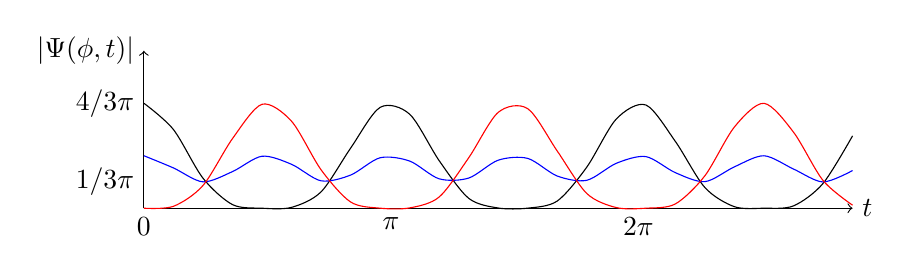
\begin{tikzpicture}
      \draw[->] (0,0) -- (9,0) node[right] {$t$};
      \draw[->] (0,0) -- (0,2) node[left] {$|\Psi(\phi,t)|$};
      \draw[domain=0:9,smooth,variable=\x,black] plot ({\x},{(1/3)*(1+cos(2*deg(\x))^2+2*cos(2*deg(\x)))});
     \draw[domain=0:9,smooth,variable=\x,blue] plot ({\x},{(1/3)*(1+cos(2*deg(\x))^2+2*cos(2*deg(\x))*cos(deg(pi/2)))});
     \draw[domain=0:9,smooth,variable=\x,red] plot ({\x},{(1/3)*(1+cos(2*deg(\x))^2+2*cos(2*deg(\x))*cos(deg(pi)))});
      \draw (0,0) node[below]{0};
      \draw (3.14,0) node[below]{$\pi$};
      \draw (6.28,0) node[below]{$2\pi$};
      \draw (0,1/3) node[left]{$1/3\pi$};
\draw (0,4/3) node[left]{$4/3\pi$};
\end{tikzpicture}
\end{center}
\end{enumerate}
\end{ans}
\newpage
\begin{qns}[Ehrenfest Theorem]\leavevmode
\begin{enumerate}[label=(\alph*)]
\item What is the commutator $[\hat{A},\hat{B}]$ of two operators $\hat{A}$ and $\hat{B}$? Use\hfill\textbf{[3]}
$$\hat{p}_x=-i\hbar\frac{\partial}{\partial x}$$
to show that $[\hat{x},\hat{p}_x]=i\hbar$. What does this imply about the measurement of position and momentum?
\item Verify the commutation relation $[\hat{A},\hat{B}\hat{C}]=[\hat{A},\hat{B}]\hat{C}+\hat{B}[\hat{A},\hat{C}]$. Using this result or otherwise show that $[\hat{x},\hat{p}_x^2]=2i\hbar\hat{p}_x$.\\[5pt]
Show that\hfill\textbf{[5]}
$$[\hat{p}_x,V(\hat{x})]=-i\hbar\frac{\partial V(\hat{x})}{\partial\hat{x}}$$
\item Write down an expression for the expectation value $\langle\hat{Q}\rangle$ of the operator $\hat{Q}$ for a system described by a normalised wavefunction $\psi$. Use the time-dependent Schrodinger equation and the Hermitian property of the Hamiltonian operator $\hat{H}$ to show that
$$\frac{d\langle\hat{Q}\rangle}{dt}=\frac{1}{i\hbar}\langle[\hat{Q},\hat{H}]\rangle$$
assuming that $\hat{Q}$ has no explicit time dependence.\hfill\textbf{[5]}
\item A particle of mass $m$ moves in one dimension in the potential $V(x)$. Write down the Hamiltonian operator and use the results above to derive expressions for $d\langle\hat{x}\rangle/dt$ and $d\langle\hat{p}_x\rangle/dt$. Comment on your results.\hfill\textbf{[7]}
\end{enumerate}
\end{qns}
\begin{ans}\leavevmode
\begin{enumerate}[label=(\alph*)]
\item $[\hat{A},\hat{B}]=\hat{A}\hat{B}-\hat{B}\hat{A}$. For some scalar function $f(x)$
$$[\hat{x},\hat{p}_x]f=x(-i\hbar)\frac{\partial f}{\partial x}-(-i\hbar)\frac{\partial(xf)}{\partial x}=i\hbar f$$
Hence, $[\hat{x},\hat{p}_x]=i\hbar$. The non-zero commutator would mean that it is impossible to measure both the position and momentum simultaneously to perfect precision. This is described in the Heisenberg Uncertainty relations
$$\Delta x\Delta p\geq\frac{1}{\hbar}|i\langle[\hat{x},\hat{p}_x]\rangle|$$
\item Simple verification:
$$[\hat{A},\hat{B}\hat{C}]=\hat{A}\hat{B}\hat{C}-\hat{B}\hat{C}\hat{A}=\hat{A}\hat{B}\hat{C}-\hat{B}\hat{A}\hat{C}+\hat{B}\hat{A}\hat{C}-\hat{B}\hat{C}\hat{A}=[\hat{A},\hat{B}]\hat{C}+\hat{B}[\hat{A},\hat{C}]$$
$$[\hat{x},\hat{p}_x^2]=[\hat{x},\hat{p}_x]\hat{p}_x+\hat{p}_x[\hat{x},\hat{p}_x]=\hat{p}_x2i\hbar$$
$$[\hat{p}_x,V(\hat{x})]=\frac{\hbar}{i}\frac{\partial V(\hat{x})}{\partial x}-V(\hat{x})\frac{\hbar}{i}\frac{\partial}{\partial x}=-i\hbar\frac{\partial V(\hat{x})}{\partial x}$$
\item The expectation value for an arbitrary operator $\hat{Q}$ is defined to be $\int\psi^*\hat{Q}\psi dx$ for some arbitrary normalized wavefunction $\psi$. Take the time derivative and use the time-dependent Schrodinger equation $i\hbar\frac{\partial\psi}{\partial t}=\hat{H}\psi$ and its Hermitian conjugate $-i\hbar\frac{\partial\psi^*}{\partial t}=\psi^*\hat{H}^\dag=\psi^*\hat{H}$ (where $\hat{H}$ is Hermitian):
$$\frac{d}{dt}\langle\hat{Q}\rangle=\int\frac{\partial\psi^*}{\partial t}\hat{Q}\psi+\psi^*\frac{\partial\hat{Q}}{\partial t}\psi+\psi^*\hat{Q}\frac{\partial\psi}{\partial t}dx=\int\frac{1}{-i\hbar}\psi^*\hat{H}\hat{Q}\psi+\psi^*\hat{Q}\frac{\hat{H}}{i\hbar}\psi+\psi^*\frac{\partial\hat{Q}}{\partial t}\psi dx=\frac{1}{i\hbar}\langle[\hat{H},\hat{Q}]\rangle$$
where $\hat{Q}$ has no explicit time-dependence as given.
\item The Hamiltonian operator is $\hat{H}=\frac{\hat{p}_x^2}{2m}+V(\hat{x})$, and so from part (c) and (b):
$$\frac{d\langle\hat{x}\rangle}{dt}=\frac{1}{i\hbar}\langle[\hat{x},\hat{H}]\rangle=\frac{1}{i\hbar}\frac{1}{2m}\langle[\hat{x},\hat{p}_x^2]\rangle=\frac{1}{2i\hbar m}\langle 2i\hbar\hat{p}_x\rangle=\frac{\langle\hat{p}_x\rangle}{m}$$
The expectation of momentum is similar to the classical definition of momentum.
$$\frac{d\langle\hat{p}_x\rangle}{dt}=\frac{1}{i\hbar}\langle[\hat{p}_x,\hat{H}]\rangle=\frac{1}{i\hbar}\langle[\hat{p}_x,V(\hat{x})]\rangle=\frac{1}{i\hbar }\bigg\langle\frac{\partial V(\hat{x})}{\partial\hat{x}}(-i\hbar)\bigg\rangle=-\bigg\langle\frac{\partial V(\hat{x})}{\partial\hat{x}}\bigg\rangle\approx-\frac{\partial V(\langle\hat{x}\rangle)}{\partial\hat{x}}$$
This approximation is valid when $\frac{(\delta x)^2}{2}V''(\langle x\rangle)$ is small.
\end{enumerate}
\end{ans}
\newpage
\subsubsection{Section C}
\begin{qns}[QM Essay]
Write an essay on the postulates of quantum mechanics and the experiments that gave rise to them. Include discussions of the photoelectric effect, the Davisson and Germer experiment, and Young’s double slit experiment.\hfill\textbf{[20]}
\end{qns}
\begin{ans}
Quantum physics was a revolution in modern physics in the 19th century. The fundamental revolution is the idea brought forth by Max Planck that electromagnetic radiation is quantized, i.e. light are packets of fixed energy called photons. To motivate this postulate, we begin with a discussion of the photoelectric effect.\\[5pt]
In 1887, Hertz discovered that the electrons were observed to be ejected from the metal when the metal was irradiated with light. Classically, we expect:
\begin{itemize}
\item Since the intensity of an electromagnetic wave is proportional to the square of its amplitude, any frequency with sufficiently high intensity can supply the necessary energy to free the electron from the metal.
\item For low intensity, an electron will keep on absorbing energy at a continuous rate and hence given sufficient amount of time, the electron will gain sufficient energy to leave the metal.
\item Electron's kinetic energy should depend on the intensity of the light source. More intense radiation will give the electron more energy.
\end{itemize}
However, the observations made were completely opposite.
\begin{itemize}
\item If the frequency of the incident radiation is smaller than the metal's threshold frequency, which is dependent on the metal, no electron can be emitted regardless of the radiation's intensity.
\item No matter how low the intensity of the incident radiation, electrons will be ejected instantly the moment the frequency of the radiation exceeds the threshold frequency of the metal.
\item The kinetic energy of the ejected electron depends on the frequency but not the intensity of the beam. In fact, the kinetic energy increases linearly with the incident frequency.
\item Moreover, at any frequency above the threshold frequency, the number of electrons ejected increases with the intensity of the light but does not depend on the light's frequency. Hence, the magnitude of the photoelectric current generated is proportional to the intensity of the light.
\end{itemize} 
Based on Planck's postulate, Einstein gave a theoretical explanation for the photoelectric effect in 1905.
\begin{itemize}
\item The incident radiation of frequency $f$ consists of photons of energy $hf$. Electrons gain energy by completely absorbing one of these photons, irrespective of the intensity of the incident radiation. This interaction can be instantaneous.
\item The threshold frequency $f_0$ of the metal is related to the work function of the metal $W$, which is defined as the minimum energy required to dislodge the electron from the metal. As long as the photon's energy is greater than the work function, the electron will be ejected. The remaining energy of the electron is the kinetic energy of the electron $K$.
$$hf=W+K=hf_0+\frac{1}{2}mv^2$$
\item The kinetic energy of the electron increases linearly with the incident frequency and is clearly independent of the intensity of the radiation. Moreover, it clearly shows that below the threshold frequency, no electron can be ejected from the metal.
\end{itemize}
Planck's postulate was relevant in other experiments and models, and has helped revolutionize our understanding of physics. Another instance is the Bohr's model where Bohr extended this idea and postulated that the angular momentum of electron's orbits are quantized. This result in discrete energy levels which accounts for the emission and absorption spectra of various chemicals, particularly Hydrogen. In these spectra, spectral lines were identified at fixed wavelengths which are explained as photon emission accompanied by the electrons transiting different energy levels.\\[5pt]
Next, we discuss the Davisson and Germer experiment to illustrate another revolution in modern physics. In 1927, Davisson and Germer scattered a $54eV$ monoenergetic beam of electrons from a Nickel crystal. The source and detector were symmetrically located with respect to the crystal's normal, similar to Bragg setup for X-ray diffraction of a crystal. Interestingly, electrons are scattered in all directions from the crystal, but a minima and maxima was found at $\theta = 35\degree$ and $\theta=50\degree$ respectively. This pattern persisted even when the intensity of the beam was so low that the incident electrons were sent one at a time. This result was very similar to Bragg's X-ray diffraction, i.e. $n\lambda=2d\sin\phi $ where $2\phi+\theta=\pi$.\\[5pt]
This result cannot be explained by the classical idea where electrons are strictly regarded as particles. The experiment thus suggested that electrons have wave-like properties. In the same year, Thomson diffracted electrons through a polycrystalline thin film and obtained diffraction rings. This result was very similar to diffracting light through the same film. Thomson thus confirm that electrons have wave-like properties.\\[5pt]
In fact, in the first decade of the 1800s, Young carried out his original double-slit experiment with light to show that the waves of light from the two slits interfered to produce a characteristic fringe pattern on a screen. Classically, we expect when both slits, in front of a source of particles, are open, the resultant intensity distribution is the sum of that corresponding to each slit. As for waves, an interference pattern is obtained since the amplitudes add and not the intensities.
$$|\psi_1+\psi_2|^2=|\psi_1|^2+|\psi_2|^2+2\text{Re}(\psi_1^*\psi_2)$$
where the last term becomes $2\sqrt{I_1I_2}\cos\delta$, where $\delta$ is the phase difference between $\psi_1$ and $\psi_2$, which results in an oscillating term. The double-slit experiment for electrons was performed by Claus J\"{o}nsson, where he demonstrated electron interference pattern for up to five slits. All these experiments suggest the idea that particles have wave-like behaviour which is apparent in the quantum regime. Since then particle interference has been demonstrated with neutrons, atoms and molecules as large as carbon-60 and carbon-70. Motivated by this dual property in light, de Broglie derived a relationship between wavelength and momentum of matter, known as the de Broglie relation.
$$p=\frac{h}{\lambda}$$
More importantly, the experiments suggest that all quantum particles could really be described by like a wave-like function, known as the wavefunction that encompasses all of its behaviour. This postulates that states of a quantum system correspond to non-zero elements of a complex vector space (Hilbert space $\mathcal{H}$) with $\psi$ and $\alpha\psi$ physically equivalent $\forall\alpha\in\mathbb{C}\backslash\{0\}$. In particular, the norm squared of the wavefunction gives the probability density.  This process of taking the square magnitude explains how this `interference' occurs, similar to that in waves:
$$|\psi_1+\psi_2|^2=|\psi_1|^2+|\psi_2|^2+2\text{Re}(\psi_1^*\psi_2)$$
\end{ans}
\newpage
\begin{qns}[QM Short Notes]
Write brief notes on two of the following:\hfill\textbf{[20]}
\begin{itemize}
    \item indistinguishable particles and consequences of their exchange;
    \item the specific heat of diatomic gases due to quantum mechanical vibrations;
    \item quantum tunneling including some experimental examples of it.
\end{itemize}
\end{qns}
\begin{ans}\leavevmode
\subsubsection*{Indistinguishable particles and consequences of their exchange:}
In classical mechanics, when a system is made of identical particles, it is possible to identify and distinguish each particle from the others. In quantum mechanics, however, identical particles are truly indistinguishable since we cannot specify more than a complete set of commuting observables, and due to uncertainty principle (path of a particle is meaningless).\\[5pt]
As an example, when scattering two identical particles in the centre of mass frame, it is impossible to forecast with certitude that the particle fired from source $S_1$ will make it to detector 1 or 2. 
\begin{figure}[H]
    \centering
    \includegraphics[width=\linewidth]{indistinguishable.PNG}
    \caption{Scattering of Indistinguishable Particles}
\end{figure}
Consider two particles with single particle basis $|\alpha\rangle$ and $|\beta\rangle$ respectively. We define the transposition operator
$$P_{12}|\alpha\rangle|\beta\rangle:=|\beta\rangle|\alpha\rangle$$
where $|\alpha\rangle|\beta\rangle=|\alpha\rangle\otimes|\beta\rangle$. Note $P_{12}\in\mathcal{L}(V\otimes V)$. The transposition operator is Hermitian, i.e. $P_{12}^\dag=P_{12}$. The eigenvalues of $P_{12}$ are $\pm1$, where $+1$ represents symmetric states and $-1$ represents anti-symmetric states.\\[5pt]
The spin-statistics theorem states that particles whose spin is an integer (half odd integer) multiple of $\hbar$ are described by totally symmetrical (anti-symmetric) states. They are bosons (fermions) and satisfy the Bose-Einstein (Fermi-Dirac statistics). Moreover, partially symmetric states do not exist. Essentially, for a system of $N$ identical particles,
$$P_{ij}|N\text{ identical bosons }\rangle=+|N\text{ identical bosons }\rangle$$
$$P_{ij}|N\text{ identical fermions }\rangle=-|N\text{ identical fermions}\rangle$$
where $P_{ij}$ is the permutation operator that interchanges the $i$th and the $j$ th particles, with $i$ and $j$ arbitrary.\\[5pt]
Consider two particles with states they can occupy be $|\alpha\rangle$ and $|\beta\rangle$. For bosons, the independent states are
$$|\alpha\rangle|\alpha\rangle,\quad|\beta\rangle|\beta\rangle,\quad\frac{1}{\sqrt{2}}(|\alpha\rangle|\beta\rangle+|\beta\rangle|\alpha\rangle)$$
For fermions, the only independent state can be written as
$$\frac{1}{\sqrt{2}}(|\alpha\rangle|\beta\rangle-|\beta\rangle|\alpha\rangle)$$
For classical particles (distinguishable), they follow the Maxwell-Boltzmann statistics. the independent states are $|\alpha\rangle|\beta\rangle$, $|\beta\rangle|\alpha\rangle$, $|\alpha\rangle|\alpha\rangle$, $|\beta\rangle|\beta\rangle$.\\[5pt]
For any two fermions, say if $\alpha=\beta$, the state vanishes, i.e. no such state exists. This is called Pauli Exclusion Principle, which states that no two fermions can occupy the same state.\\[5pt]
We generalize this to $N$ identical particles. For a system of many identical particles, we can define
$$P_{ij}|k^1\rangle|k^2\rangle...|k^i\rangle|k^{i+1}\rangle...|k^j\rangle...:=|k^1\rangle|k^2\rangle...|k^j\rangle|k^{i+1}\rangle...|k^i\rangle...$$
It is clear that $P_{ij}^2=1$ and the allowed eigenvalues are $\pm 1$ as well. Also, $[P_{ij},P_{kl}]\neq 0$. The normalization is $\sqrt{\prod_{i=1}^nN_i!/N!}$ where $N$ is the total number of particles and $N_i$ is the number of times $|k^{(i)}\rangle$ occurs. For $N$ particle systems, we can define $N!$ permutation operators. To build an anti-symmetric $N$ particle states, we use the Slater determinant (determinant ensures exchange of any two particles will give a minus sign).\\[5pt]
The total wavefunction may be written as a product of spatial $\psi(\mathbf{r_i})$ and spin wavefunction $\chi(\mathbf{m_{s_i}})$. We denote it as $|\Psi\rangle\in V\otimes W$, where $V$ and $W$ are spaces for spatial and spin states respectively. The overall state must satisfy the symmetrization postulate. Say if the overall state must be antisymmetric, then either spatial or the spin state must be symmetric, with the other being antisymmetric.
\subsubsection*{The specific heat of diatomic gases due to quantum mechanical vibrations:}
For a diatomic gas, its vibrational motion is the same as that of a single mass moving in a central potential (quadratic for low energies). Classically, each degree of freedom (vibrational mode) has thermal energy $0.5k_BT$. Quantum mechanically, an oscillator has a range of discrete vibrational energy states with $E_n=(n+0.5)\hbar\sqrt{\alpha/\mu}$ where $\mu$ is the reduced mass of the diatomic molecule and $\alpha$ is the stiffness of the chemical bond. The average vibrational energy per molecule is
$$\langle E\rangle=\frac{1}{2}\hbar\omega+\frac{\sum_{n=1}^\infty n\hbar\omega e^{-n\hbar\omega\beta}}{\sum_{n=1}^\infty e^{-n\hbar\omega\beta}}$$
To solve that summation, let $Z=\sum_{n=1}^\infty e^{-n\hbar\omega\beta}=\frac{1}{1-e^{-\hbar\omega\beta}}$ be the partition function. We have
$$-\frac{\partial Z}{\partial\beta}=\sum_{n=1}^\infty n\hbar\omega e^{-n\hbar\omega\beta}=\frac{\hbar\omega e^{-\hbar\omega\beta}}{(1-e^{-\hbar\omega\beta})^2}$$
so $\langle E\rangle=0.5\hbar\omega+\frac{\hbar\omega}{e^{\hbar\omega\beta}-1}$, where the second term is the average energy of a quantum SHO lightly coupled to a heat bath of temperature $T$. The vibrational heat capacity of $N$ diatomic molecules is
$$C_{vib}=N\frac{\partial\langle E\rangle}{\partial T}=Nk_B\frac{\hbar^2\omega^2}{k_B^2T^2}\frac{e^{\hbar\omega/k_BT}}{(e^{\hbar\omega/(k_BT)}-1)^2}$$
$C_{vib}\rightarrow NK_B$ as $T\rightarrow\infty$. It approaches the classical value at the temperature $\hbar\omega/k_B$.
\newpage
\subsubsection*{Quantum tunneling including some experimental exampels of it:}
The following describes a potential barrier
   $$
V(x)=
\left\{
        \begin{array}{ll}
      U & 0<x<a\\
	0& x\leq 0,x\geq a\\
        \end{array}
    \right.
$$
Define $E$ and $U$ such that
$$E=\frac{\hbar^2k^2}{2m},\quad U-E=\frac{\hbar^2\kappa^2}{2m}$$
and consider scattering states of energies $0<E<U$. We guess a wavefunction of the form
       $$
\psi(x)=
\left\{
        \begin{array}{ll}
      Ie^{ikx}+Re^{-ikx} & x<0\\
 Te^{ikx}& x>0\\
 Ae^{\kappa x}+Be^{-\kappa x}&0<x<a
        \end{array}
    \right.
$$
Invoke continuity condition of $\psi$ and $\psi'$ at the points od potential discontinuity $x=0$ and $x=a$:
$$I+R=A+B,\quad ik(I-R)=k(A-B)$$
$$Ae^{\kappa a}+Be^{-\kappa a}=Te^{ika},\quad \kappa (Ae^{\kappa a}-Be^{-\kappa a})=ikTe^{ika}$$
Solve them to get 
$$I+\frac{\kappa\mp ik}{\kappa\pm ik}R=Te^{ika}e^{\mp\kappa a}\implies T=Ie^{-ika}\frac{1}{\cosh\kappa a-i\frac{k^2-\kappa^2}{2k\kappa}\sinh ka}$$
Define the probability current to be
$$J(x,t)=-\frac{i\hbar}{2m}\bigg(\Psi^*\frac{\partial\Psi}{\partial x}-\frac{\partial\Psi^*}{\partial x}\Psi\bigg)\in\mathbb{R}$$
then the currents will be
       $$
J(x)=
\left\{
        \begin{array}{ll}
      J_{inc}+J_{ref}=\frac{\hbar k}{m}(|I|^2-|R|^2)& x<0\\
J_{tr}=|T|^2\frac{\hbar k}{m}& x>0\\
        \end{array}
    \right.
$$
and thus the probability of transmission is
$$P_{tr}=\frac{|J_{tr}|}{|J_{inc}|}=\frac{|T|^2}{|I|^2}=\frac{1}{1+\frac{U^2\sinh^2\kappa a}{4E(U-E)}}$$
This is the phenomenon of quantum tunnelling where there is non-zero probability of passing through the barrier even though it classically does not have enough energy. For $\kappa a>>1$, the probability decays as $e^{-2\kappa a}$. Next, we proceed to discuss a few experimental evidences of quantum tunnelling.\\[5pt]
Under normal circumstances, a low-energy electron cannot leave the surface of a metal because of the Coulombic interaction between the electron and the ions that make up the lattice.
The presence of an external electric field ($V =-Ex$) creates a potential having the form of a narrow barrier. Electrons can tunnel across this barrier giving rise to a process known as field emission. This process has been developed into the scanning tunneling microscope (STM).\\[5pt]
In the STM, a sharp tip is scanned over the surface the sample, and a voltage is applied such that field emission occurs. The tunneling current, which is exponentially dependent on spacing, is used to hold the tip at a fixed height above the surface. The feedback control to the piezo displacer is then used as a measure of the height of the surface.\\[5pt]
Another evidence is in radioactive decay. Large unstable nuclei can decay via the emission of an $\alpha$-particle, which is the nucleus of a He atom comprising two protons and two neutrons. The energy of the emitted $\alpha$-particle is small (4-9 MeV) compared with the nuclear barrier (20-25 MeV). The transmission probability, and therefore the rate of escape, depends near-exponentially on the kinetic energy of the released particle. Small changes in the energy of the released particle correspond to very large changes in the materials half life. A high-energy particle has a small half life.\\[5pt]
A similar example would be nuclear fusion in stars. Proton-proton chain rapidly occurs between positively-charged protons despite the large Coulomb barrier. This is because tunneling may occur, allowing a reaction to take place despite not having sufficient energy to overcome the Coulomb barrier, i.e. the star is not hot enough.
\end{ans}
\newpage
\subsubsection{Section D}
\begin{qns}[Chi Squared]\leavevmode
\begin{enumerate}[label=(\alph*)]
\item Explain how the $\chi^2$ test can help to determine if a theoretical model fits a set of experimental data.\hfill\textbf{[6]}
\item An experiment measures the radiation emitted by a radioactive source passing through an increasing number of sheets, $n$, composed of a certain material. Each measurement lasts for 1 s and yields the results listed in the table below.
\begin{center}
\begin{tabular}{ |c|c|c|c|c|c|c|c|c|}
\hline
number of sheets, $n$ & 1 & 2 & 3 & 4 & 5 & 6 & 7 &8 \\
\hline
counts in 1 s & 723 & 244 & 95 & 35 & 8 & 5 &6 &5\\
\hline
\end{tabular}
\end{center}
Plot the counts as a function of $n$ to show that the count rate is proportional to
$$N_0e^{-nb}$$
where $N_0 = 2018.5$ counts s$^{-1}$ and the parameter $b$ is a material dependent constant. State over which range of $n$ this model describes the data.\hfill\textbf{[3]}
\item $N_0$ was determined from a 1000 s long measurement for $n = 0$. Estimate the respective errors in $N_0$ and in the counts given in the table above. Comment on the accuracy of the two measurements.\hfill\textbf{[2]}
\item The value $b$ of the sheet material is known to be either $b = 1$ or $b = 1.1$. Perform the $\chi^2$ test to determine which value of b provides a better fit to the data.\hfill\textbf{[7]}
\item How should the model be modified to account for the discrepancy between the expected and measured counts?\hfill\textbf{[2]}
\end{enumerate}
\end{qns}
\begin{ans}\leavevmode
\begin{enumerate}[label=(\alph*)]
\item If we have a set of data in the form of a certain number of observations within a given number of bins, and a model that predicts what the observed distribution should be, then under the assumptions
\begin{itemize}
    \item assume no errors on the inputs;
    \item assume errors on the outputs are independent between observations.
\end{itemize}
We may use the $\chi^2$ test to determine goodness-of-fit. The statistic $\chi^2$ is then
$$\chi^2=\sum_{bins}\bigg(\frac{N_{obs}-N_{pred}}{\sigma_{pred}}\bigg)^2$$
The expected value of $\chi^2$ is the degrees of freedom of the data, $N$, which is the number of data points (bins) minus the number of parameters from the model. If $\chi^2$ is significantly higher than $N$, then the discrepancies between the model and data are unlikely to be explained by random statistical fluctuations in sample distribution. Instead, this arise from either
\begin{itemize}
    \item an incorrect null hypothesis, i.e. data cannot be described by the model, or
    \item an incorrect assumption on the errors.
\end{itemize}
If $\chi^2$ is instead lower than $N$, it is indicative that we have overestimated the degrees of freedom in the model (e.g. the errors are correlated between experiments, the experimentalists forged the data, or maybe parameters in the model were not independent, for instance, $y=(x-a)^2$ and $y=x^2+\alpha x+\beta$ are both quadratic models but with different degrees of freedom).\\[5pt]
If the number of counts in any given bin is a rate process, then it obeys Poisson statistics, and hence the predicted standard deviation will be equal to the square root of the predicted number of counts, i.e.
$$\chi^2=\sum_{bins}\frac{(N_{obs}-N_{pred})^2}{N_{pred}}$$
If our bins are such that the predicted number of occurrences is too small (fewer than 5), then we must amalgamate the bins with nearby bins to avoid an undesirably large $\chi^2$ value.
\item Let the number of counts in 1 seconds be $R$. Plot $\ln(R)=\ln(N_0)-nb$. The trendline of the negative slope is valid up to about $n=5$.
\begin{figure}[H]
    \centering
    \includegraphics[scale=0.75]{2018P1D12.PNG}
    \caption{Best fit line for up to $n=5$ (red) and for entire data set (blue).}
\end{figure}
\item Since we are counting the number of events $N$ in a time period $T$, then this is a Poisson process. Let $\mathcal{N}:=\frac{N}{T}$, then $\sigma_{\mathcal{N}}=|\frac{\sigma_N}{T}|=\frac{\sqrt{N}}{T}=\sqrt{\frac{\mathcal{N}}{T}}$. The error in $\mathcal{N}=N_0$ is $\sqrt{2018.5/1000}=1.4$. The error in counts will be 
\begin{itemize}
    \item $n=1$: $\sqrt{723}\approx 26.89$;
    \item $n=2$: $\sqrt{244}\approx 15.62$;
    \item $n=3$: $\sqrt{95}\approx 9.747$;
    \item $n=4$: $\sqrt{35}\approx 5.92$;
    \item $n=5$: $\sqrt{8}\approx 2.8284$;
    \item $n=6$: $\sqrt{5}\approx 2.236$;
    \item $n=7$: $\sqrt{6}\approx 2.449$;
    \item $n=8$: $\sqrt{5}\approx 2.236$
\end{itemize}
$N_0$ was measured over a longer time period (1000 s) compared to 1 s, which is 1000 times longer. Hence, the accuracy is $\sqrt{1000}$ times greater.
\item Since the first five data points are valid in the linear regime, we perform $\chi^2$ test on these.\\[5pt]
For $b=1$, $R=2018.5 e^{-n}$, we have
$$\chi^2=\frac{(742.56-723)^2}{742.50}+\frac{(273.17-244)^2}{273.17}+\frac{(100.5-95)^2}{100.50}+\frac{(36.97-35)^2}{36.97}+\frac{(13.60-8)^2}{13.60}=6.34$$
For $b=1.1$, $R=2018.5 e^{-1.1n}$, we have
$$\chi^2=\frac{(671.90-723)^2}{671.90}+\frac{(223.66-244)^2}{223.66}+\frac{(74.45-95)^2}{74.45}+\frac{(24.78-35)^2}{24.78}+\frac{(8.25-8)^2}{8.25}=15.63$$
$\chi^2$ should be expected to be 5 with standard deviation $\sim\sqrt{2\times 5}=3.16$. Hence, $b=1$ is favoured over $b=1.1$.
\item The model should be modified to $R=Ae^{-nb}+B$, where $N_0=A+B$ is the mean background radiation.
\end{enumerate}
\end{ans}
\newpage
\begin{qns}[Expt Mthds Short Notes]
Write brief notes on two of the following:\hfill\textbf{[20]}
\begin{itemize}
    \item the use of Bayes’ theorem and prior knowledge;
    \item systematic errors and techniques for their removal;
    \item the origin of thermal (Johnson) and shot noise.
\end{itemize}
\end{qns}
\begin{ans}\leavevmode
\subsubsection*{The use of Bayes' theorem and prior knowledge:}
Prior to the experiment, one usually has some prejudice as to the values of the model parameters, either on the basis of someone's else data or some other information. This is captured by $p($ model parameters $)$, which is known as the prior probability, i.e. our knowledge of the model parameters prior to performing the experiment. After the experiment, the extent to which certain model parameters are to be preferred will depend on whether the data measured could reasonably have been explained on the basis of those parameter values, which is captured by the likelihood function, $p($ Data| Model parameters $)$. By Bayes' Theorem, the posterior probability, i.e. our knowledge of the model parameters after performing the experiment, is
$$p(\text{ model parameters | Data })=\frac{p(\text{ Data | model parameters})\times p(\text{ model parameters })}{p(\text{Data})}$$
In the case of a uniform prior in the model parameters, the Bayesian parameter estimation is equivalent to the maximum likelihood approach where we find the value of the vector of model parameters $\mathbf{a}$ that maximizes the likelihood function $\mathcal{L}(y_1,...,y_N|\mathbf{a})$. But $\mathcal{L}(y_1,...,y_N|\mathbf{a})$ measures $p(\text{data}|\mathbf{a})$, which is different from what we want, i.e. $p(\mathbf{a}|\text{data})$. 
\subsubsection*{Systematic errors and techniques for their removal:}
Systematic errors are broadly due to (i) inaccurate instruments, (ii) apparatus that differs from some assumed form, (iii) incorrect theory, that is, there are some effects present that are not taken into account. It is a good rule that whenever there is an apparent symmetry in the apparatus, reversing some quantity or interchanging any two components should in theory have no effect.
\begin{itemize}
    \item Study the equipment and measurement instruments beforehand to identify any zero errors and correct for them. Also, calibrate the instruments. If necessary, measure the same quantity with different equipment that may have been calibrated differently.
    \item Check the experimental set-up by measuring different quantities to make sure they are consistent with the desired experimental setup.
    \item Null methods can be used, where the indicating device need not be linear or well-calibrated and we attempt to make a measurement based on the indicating device coming to a null state.
    \item We can make the same measurement at different times to observe if there are any changes (or gradual drift) in the measured quantity due to environmental changes (ambient temperature) or changes in equipment (overheating) over time.
    \item We can make differential (difference) measurements so that the systematic error is cancelled out in the calculations.
\end{itemize}
\newpage
\subsubsection*{The origin of thermal (Johnson) and shot noise:}
Johnson noise is the thermally induced noise that is present in any resistive element. It is the electronic analogue of the random motion of gas molecules in a box, which is known as Brownian motion. In noise terminology, Johnson noise is white noise which is noise power per unit frequency that is independent of frequency, i.e. flat frequency spectrum. In fact, the Johnson noise is independent of the design of the resistive elements, and represents noise we could never eliminate.\\[5pt]
Shot Noise is present in any circuit that carries a current. Current is composed of discrete charges arriving at random times. Given that each arrival pulse is very short, the power spectrum against frequency is uniform,, i.e. `white noise': Poisson noise of a time-varying signal is spread over all temporal frequencies. A current $I$ consists of a flow of electrons of the form $I=e\langle N\rangle$, where $\langle N\rangle$ is the average number of electrons passing through a plane normal to the electron flow per unit time. However, during any given time interval, not necessarily exactly $\langle N\rangle$ electrons will pass the reference point. The distribution about $\langle N\rangle$ is given by $\langle N\rangle^{0.5}$, as for any statistical process (Poissonian process). This noise is a direct result of the quantization of the electric change and is given by r.m.s. value $\sqrt{2eIN}$.
\end{ans}
\newpage
\subsection{Paper 2}
\subsubsection{Section A}
\begin{qns}[Resolution]
The Hubble space telescope has a primary mirror of 2.4 m diameter. Estimate the angular resolution in radians at a photon energy of 2.5 eV. What is the resolution in metres when observing a source at a distance of 2$\times10^{17}$ m?\hfill\textbf{[4]}
\end{qns}
\begin{ans}
The Rayleigh limit is $$\Delta\theta=1.22\frac{\lambda}{D}=\frac{1.22hc}{ED}=\frac{1.22(6.626\times10^{-34})(3\times10^8)}{(2.5)(1.6\times10^{-19})(2.4)}=2.4\times10^{-7}rad$$
Then, $d=L\Delta\theta=2\times10^{17}\times 2.4\times10^{-7}=4.9\times10^{10}$ m. 
\end{ans}
\begin{qns}[Fresnel Diffraction]
A diffraction pattern is observed at 0.5 m from an aperture. What is the outer radius of the second Fresnel half-period zone at the aperture, if the aperture is positioned at 0.5 m from a monochromatic point source of wavelength 400 nm?\hfill\textbf{[4]}
\end{qns}
\begin{ans}
The radius of the $n$th half-period zone is $r_n=\sqrt{nR\lambda}$, where $R$ is the harmonic mean of the source-aperture and aperture-sreen distance, i.e. $(\frac{1}{0.5}+\frac{1}{0.5})^{-1}=0.5$, and so $r_2=\sqrt{2(400\times10^{-9})(0.5)}=4.5\times10^{-4}$ m.
\end{ans}
\begin{qns}[Impedance]
To perform ultrasound imaging, an acoustic wave is transmitted into the body and reflections are detected at the surface of the body. By calculating the energy transmitted at an air-body boundary and a water-body boundary, explain why water-based gel is applied to the body surface during ultrasound imaging.\hfill\textbf{[4]}
\begin{mdframed}
You may assume acoustic impedances of: $Z_{air} = 4 \times10^2$ kg m$^{-2}$ s$^{-1}$, $Z_{water} = 1.48 \times10^6$ kg m$^{-2}$ s$^{-1}$and $Z_{body} = 1.63 \times 10^6$ kg m$^{-2}$ s$^{-1}$.
\end{mdframed}
\end{qns}
\begin{ans}
The reflection intensity coefficient $R$ is $ R=\bigg|\frac{1-\frac{Z_2}{Z_1}}{1+\frac{Z_2}{Z_1}}\bigg|^2$. $\frac{Z_2}{Z_1}$ for the air-body boundary is $\frac{1.63\times10^6}{4\times10^2}=4075$, with $R=0.99902$ and hence $T=1-0.999=0.00098$. $\frac{Z_2}{Z_1}$ for the water-body boundary is $\frac{1.63}{1.48}=1.10$, with $R=0.023$ and hence $T=1-0.023=0.998$. At a given level of transmitted power, the initial signal can be about 1000 times weaker with a gel interface.
\end{ans}
\begin{qns}[Phonons]
Draw labelled diagrams showing the phonon dispersion curves for a solid modelled as a) a monatomic chain and b) a diatomic chain where the atoms are i) of the same mass and ii) of different masses. Indicate the position of the first Brillouin zone boundary in each case.
\end{qns}
\begin{ans}
Let $a$ be the interatomic spacing. $q=\pm\frac{\pi}{a}$ is the Brillouin Zone edge. With a diatomic chain, we have double the unit cell length in real space, so the momentum space has halved the period. For equal mass diatomic, the gap at the zone boundary closes, i.e. bandgap only exist for diatomic chain. Below shows the dispersion curves for monatomic (left) and diatomic (right) with the optical (red) and acoustic (blue) branches.
\begin{center}
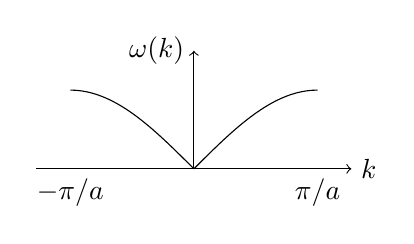
\begin{tikzpicture}
      \draw[->] (-2,0) -- (2,0) node[right] {$k$};
      \draw[->] (0,0) -- (0,1.5) node[left] {$\omega(k)$};
      \draw[domain=0:1.57,smooth,variable=\x,black] plot ({\x},{sin(deg(\x))});
      \draw[domain=-1.57:0,smooth,variable=\x,black] plot ({\x},{-sin(deg(\x))});
      \draw (1.57,0) node[below]{$\pi/a$};
      \draw (-1.57,0) node[below]{$-\pi/a$};
\end{tikzpicture}
\hfill{}
\begin{tikzpicture}
      \draw[->] (-2,0) -- (2,0) node[right] {$k$};
      \draw[->] (0,0) -- (0,4) node[left] {$\omega(k)$};
      \draw[domain=0:1.57,smooth,variable=\x,red] plot ({\x},{2*sqrt(0.5*(1+2+sqrt((1-2)^2+2*(cos(deg(\x))^2))))});
      \draw[domain=-1.57:0,smooth,variable=\x,red] plot ({\x},{2*sqrt(0.5*(1+2+sqrt((1-2)^2+2*(cos(deg(\x))^2))))});
      \draw[domain=-1.57:0,smooth,variable=\x,blue] plot ({\x},{-2*sin(deg(\x))});
      \draw[domain=0:1.57,smooth,variable=\x,blue] plot ({\x},{2*sin(deg(\x))});
      \draw (1.57,0) node[below]{$\pi/2a$};
      \draw (-1.57,0) node[below]{$-\pi/2a$};
\end{tikzpicture}
\end{center}
\end{ans}
\begin{qns}[Transport]
Given a Hall coefficient of $2.4\times10^{-10}$ m$^3$ C$^{-1}$,  calculate the number of carriers per atom for Beryllium of density 1.85 g cm$^{-3}$ and relative atomic mass 9. Suggest an interpretation of your result.
\end{qns}
\begin{ans}
For the Hall setup, we have the electric field $E$, magnetic field $B$ and current density $J$ to be mutually orthgoonal. So, the Hall coefficient is $R_H=\frac{E}{JB}=\frac{1}{nq}$, where $q$ is the (signed) particle charge present in the current. Since for Be, $R_H>0$, the holes dominate charge. The number density of the charge is $\frac{1.85\times10^3}{9\times 1.66\times10^{-27}}=10^{29}$ m$^{-3}$, where the density in kg m$^{-3}$ is 1.85$\times10^3$. The valency is thus
$$\frac{1}{nR_He}=\frac{1}{10^{29}(2.4\times10^{-10})(1.6\times10^{-19})}=0.26$$
\end{ans}
\subsubsection{Section B}
\begin{qns}[Oscillation]
A damped simple-harmonic oscillator has an equation of motion
$$\ddot{x}+\gamma\dot{x}+\omega_0^2x=0$$
where $x$ is the displacement from equilibrium, $m$ the mass, $\gamma=b/m$ the friction coefficient and $\omega_0=\sqrt{k/m}$ the resonant angular frequency.
\begin{enumerate}[label=(\alph*)]
\item By substituting a solution of the form $Ae^{pt}$ for $t > 0$, identify the conditions for heavy, critical and light damping in terms of $\gamma/m$ and $\omega_0$.\hfill\textbf{[4]}
\item The oscillator is now driven by $\text{Re}[\frac{F_0}{m}e^{i\omega t}]$, where $F_0$ is the driving force and $m$ the mass. By substituting the trial solution $x=\text{Re}[Ae^{i\omega t}]$ into the equation of motion for a damped, driven, simple-harmonic oscillator, show that $A=R(\omega)F_0$ where $R(\omega)$ is the response function \hfill\textbf{[6]}
$$R(\omega)=\frac{1}{m[(\omega_0^2-\omega^2)+i\gamma\omega]}$$
Draw an annotated sketch of the amplitude and phase of the response function as a function of frequency $\omega$. How would the amplitude sketch be modified for an oscillator with (i) a large $Q$ factor or (ii) a very small $Q$ factor?
\item For the circuit shown below, in which $V(t) = \text{Re}[V_0e^{i\omega t}]$, show that the equation for the charge, $q$, on the capacitor is\hfill\textbf{[3]}
\begin{figure}[H]
    \centering
    \includegraphics[scale=0.7]{2018P2B6Q.PNG}
\end{figure}
$$\ddot{q}+\frac{R}{L}\dot{q}+\frac{q}{LC}=\frac{V}{L}$$
\item Show that the angular frequency at which the maximum amplitude occurs is\hfill\textbf{[5]}
$$\omega_{res}=\sqrt{\frac{1}{LC}-\frac{R^2}{2L^2}}$$
\item Why is the bandwidth of this resonance independent of capacitance? How can the performance of the circuit as a narrow linewidth band-pass filter be optimised?\hfill\textbf{[2]}
\end{enumerate}
\end{qns}
\newpage
\begin{ans}\leavevmode
\begin{enumerate}[label=(\alph*)]
\item Substitute $x=Ae^{p t}$, then $p^2+\gamma p+\omega_0^2=0\implies p=\frac{-\gamma\pm\sqrt{\gamma^2-4\omega_0^2}}{2}$. 
\begin{itemize}
    \item When $\gamma^2-4\omega_0^2>0$, there are two solutions to $p$, i.e. $p_\pm=\frac{-\gamma\pm\sqrt{\gamma^2-4\omega_0^2}}{2}$, such that the resulting motion is $x(t)=c_1e^{p_+t}+c_2e^{p_-t}$. This is heavy damping, where there is no oscillation and the displacement goes asymptotically to zero. 
    \item When $\gamma^2-4\omega_0^2=0$, there is only one solution to $p$, $p=-0.5\gamma$, such that the resulting motion is $x(t)=(c_3+c_4t)e^{-0.5\gamma t}$. This is critical damping, where no oscillation occurs and the system quickly reaches equilibrium (the fastest out of the three). 
    \item When $\gamma^2-4\omega_0^2<0$, there are two solutions to $p$, i.e. $p_\pm=-\frac{\gamma}{2}\pm i\frac{\sqrt{4\omega_0^2-\gamma^2}}{2}:=-\Gamma\pm i\Omega$ such that the resulting motion is $x(t)=e^{-\Gamma t}(c_5\cos\Omega t+c_6\sin\Omega t)$. This is light damping, where the displacement oscillates (but oscillating period is slightly longer than the free oscillation case) and there is an exponential decay in amplitude.
\end{itemize}
\item The right side is now $\text{Re}[\frac{F_0}{m}e^{i\omega t}]$. We substitute $x=\text{Re}[Ae^{i\omega t}]$, we get
$$-\omega^2Ae^{i\omega t}+i\omega\gamma Ae^{i\omega t}+\omega_0^2Ae^{i\omega t}=\frac{F_0}{m}e^{i\omega t}\implies A=\frac{F_0}{m(\omega_0^2-\omega^2)+i\gamma\omega}$$
We obtain the desired form for $R(\omega)$ after using $A=R(\omega)F_0$. We see that the peak of $R(\omega)$ is
$$0=\frac{d}{d\omega}|R(\omega)|=-\frac{1}{2}\frac{-4\omega(\omega_0^2-\omega^2)+2\omega\gamma^2)}{[(\omega^2-\omega_0^2)^2+\omega^2\gamma^2]^{3/2}}$$
which give solutions $\omega=0$, $\omega=\infty$ and $\omega=\sqrt{\omega_0^2-0.5\gamma^2}$. There are no real solutions for $\omega_0\leq\frac{1}{\sqrt{2}}\gamma$ (heavy damping and critical damping). A higher $Q$ factor would mean smaller $\gamma$, and so the higher the amplitude and the resonant peak $\omega_{res}=\sqrt{\omega_0^2-0.5\gamma^2}$ approaches $\omega_0$. No resonance is achieved for $\gamma\geq2$ (regimes that are not light damping).\\[5pt]
The argument for $R(\omega)$ is $-\tan^{-1}\frac{\omega\gamma}{\omega_0^2-\omega^2}$ $\forall\gamma$. Then, $\text{arg}(R(\omega=\omega_0))=-\frac{\pi}{2}$, $\text{arg}(R(\omega=0))=0$ and $\text{arg}(R(\omega=\infty))=-\pi$. For high $Q$ factors, the phase behave almost like a step function. Below we plot the curves for increasing damping $\gamma$ (of the order black, blue, red).
\begin{center}
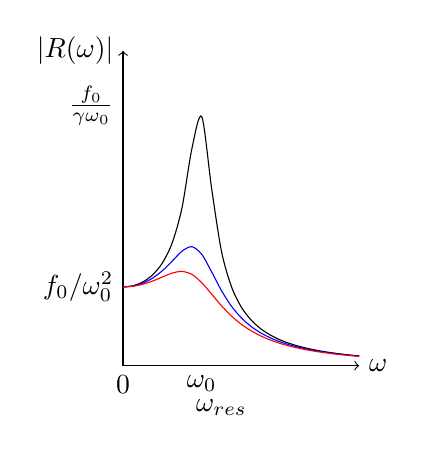
\begin{tikzpicture}
      \draw[->] (0,0) -- (3,0) node[right] {$\omega$};
      \draw[->] (0,0) -- (0,4) node[left] {$|R(\omega)|$};
      \draw[domain=0:3,smooth,variable=\x,black] plot ({\x},{1/sqrt((1-\x^2)^2+0.1*\x^2)});
      \draw[domain=0:3,smooth,variable=\x,blue] plot ({\x},{1/sqrt((1-\x^2)^2+0.5*\x^2)});
      \draw[domain=0:3,smooth,variable=\x,red] plot ({\x},{1/sqrt((1-\x^2)^2+0.9*\x^2)});
      \draw (0,0) node[below]{0};
\draw (0,1) node[left]{$f_0/\omega_0^2$};
\draw (1,0) node[below]{$\omega_0$};
\draw (1.25,-0.3) node[below]{$\omega_{res}$};
\draw (0,3.3) node[left]{$\frac{f_0}{\gamma\omega_0}$};
\end{tikzpicture}
\hspace{3cm}
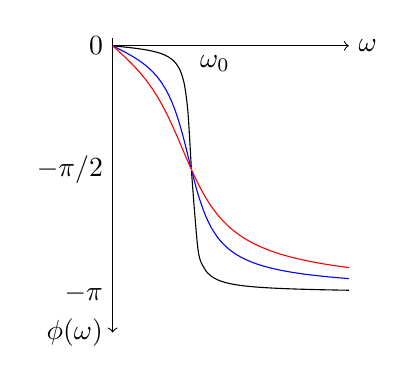
\begin{tikzpicture}
      \draw[->] (0,0) -- (3,0) node[right] {$\omega$};
      \draw[->] (0,0.1) -- (0,-pi-0.5)  node[left] {$\phi(\omega)$};
      \draw[domain=0:0.999,smooth,variable=\x,black] plot ({\x},{rad(atan(-0.1*\x/(1-\x^2)))});
      \draw[domain=1.001:3,smooth,variable=\x,black] plot ({\x},{rad(atan(-0.1*\x/(1-\x^2)))-pi});
      \draw[domain=0:0.999,smooth,variable=\x,blue] plot ({\x},{rad(atan(-0.5*\x/(1-\x^2)))});
      \draw[domain=1.001:3,smooth,variable=\x,blue] plot ({\x},{rad(atan(-0.5*\x/(1-\x^2)))-pi});
      \draw[domain=0:0.999,smooth,variable=\x,red] plot ({\x},{rad(atan(-0.9*\x/(1-\x^2)))});
      \draw[domain=1.001:3,smooth,variable=\x,red] plot ({\x},{rad(atan(-0.9*\x/(1-\x^2)))-pi});
      \draw (0,0) node[left]{0};
      \draw (0,-pi/2) node[left]{$-\pi/2$};
      \draw (0,-pi) node[left]{$-\pi$};
    \draw (1.3,0) node[below]{$\omega_0$};
\end{tikzpicture}
\end{center}
\item By Kirchoff's Voltage law,
$$V=IR+L\frac{dI}{dt}+\frac{q}{C}=\frac{dq}{dt}R+L\frac{d^2q}{dt^2}+\frac{q}{C}$$
and we obtain our desired differential equation.
\item Here, $\gamma=\frac{R}{L}$ and $\omega_0=\frac{1}{\sqrt{LC}}$. Invoking an earlier result, $\omega_{res}=\sqrt{\omega_0^2-0.5\gamma^2}=\sqrt{\frac{1}{LC}-\frac{R^2}{2L^2}}$.
\item By considering the half-power points, the bandwidth for this circuit is $\frac{2R}{L}$. To reduce the bandwidth, we either reduce $R$ or increase $L$.
\end{enumerate}
\end{ans}
\newpage
\begin{qns}[Fraunhofer Diffraction]\leavevmode
\begin{enumerate}[label=(\alph*)]
\item With the aid of a diagram, state the condition for Fraunhofer diffraction and detail the ways in which this condition can be achieved in practice.\hfill\textbf{[4]}
\item The Fraunhofer integral is given by: \hfill\textbf{[4]}
$$\psi_P\propto\int\int_\Sigma\psi_\Sigma h(x,y)e^{-ik(x_0x+y_0y)/R}dxdy$$
Define the variables in this equation and, using your diagram, outline how it is derived.
\item Two narrow slits are separated by distance $D$ and illuminated by light at a wavelength of 400 nm. Sketch the intensity of the diffraction pattern of these slits as a function of angle viewed on a distant screen. What is the angular separation of the fringes if $D = 0.1$ mm?\hfill\textbf{[3]}
\item One slit is now covered by a piece of glass that shifts the phase of the incident light by $\pi$. Sketch the new intensity diffraction pattern and annotate with the new angular separation.

\hfill\textbf{[3]}
\item The pair of narrow slits is replaced with two long rectangular apertures of width $a$ separated by $D$. The same piece of glass is placed so as to cover the left hand aperture. Show that the resulting intensity diffraction pattern has an angular dependence proportional to
$$\sin^2(qD/2)\sinc^2(qa/2)$$
where $q=\frac{2\pi}{\lambda}\sin\theta$. How does this relate to the result for two narrow slits?\\[5pt]
Sketch the resulting intensity diffraction pattern, annotating the positions of the angular minima for $D = 0.1$ mm and $a = 0.02$ mm.\hfill\textbf{[6]}
\end{enumerate}
\end{qns}
\begin{ans}\leavevmode
\begin{enumerate}[label=(\alph*)]
\item Let the source be on axis, perpendicular to the aperture plane $\Sigma$ at distance $s$. The separation of aperture plane to the screen is $L$. The Fraunhofer regime occurs when the phase variation along the aperture plane is linear. This occurs when the source and the screen is a large distance from $\Sigma$.\\[5pt]
Another way to implement this without such inconvenience is to use lenses on either side of $\Sigma$ to convert the diverging beam from the source into a parallel beam, and to focus the diffracted parallel beams onto an observation screen respectively. The source and observation screen must be placed at the object and image plane of the lenses, which are conjugate points. In this way, placing an aperture anywhere along the optical axis will produce a Fraunhofer diffraction pattern in the image plane.
\item Consider a point source of light with amplitude $a_S$. The aperture plane allows light at various points $(x,y)$ to pass through to an observer at $(x_0,y_0)$ on an observation screen. Let $|h|$ be the fraction of the magnitude of incident light being transmitted through the aperture plane and phase $\alpha=\text{arg}(h)$ imparted to the transmitted light.\\[5pt]
By Huygen's principle, light from the source reaches the aperture plane acquires a factor of $K(\theta)\frac{e^{iks}}{s}$, where $K(\theta)$ is the obliquity factor. After which, it gains another factor of $\frac{e^{ikr}}{r}K(\phi)$. Hence, the individual contribution to the observation point is $\frac{e^{iks}}{s}K(\theta)h(x,y)dxdy\frac{e^{ikr}}{r}K(\phi)$. Approximate $K(\theta)\approx 1$ and $K(\phi)\approx 1$, and assert that over the region of the aperture plane where $|h|\neq 0$, that $\frac{\Delta r}{r}<<1$ and $\frac{\Delta s}{s}<<1$, then $\frac{1}{r}$ and $\frac{1}{s}$ can be treated as constants. Upon integrating over the aperture,
$$\psi(x_0,y_0)=\frac{1}{rs}\int\int_\Sigma a_Sh(x,y)e^{iks}e^{ik\sqrt{(x-x_0)^2+(y-y_0)^2+L^2}}dxdy\approx\frac{1}{rs}\int\int_\Sigma a_Sh(x,y)e^{iks}e^{kR(1-2\frac{xx_0+yy_0}{2R^2})}dxdy$$
where $R^2=x_0^2+y_0^2+L^2$ and assume $R>>x,y,x_0,y_0$.
\item The aperture function is proportional to $h(x)=\delta(x-0.5D)+\delta(x+0.5D)$. We have
$$\psi_P\propto\int_{-\infty}^\infty[\delta(x-0.5D)+\delta(x+0.5D)]e^{-iqx}dx\propto e^{-iqD/2}+e^{iqD/2}\propto\cos(qD/2)$$
Hence, $I(\theta)\approx I_0\cos^2(q\pi D\theta/\lambda)$, where by small angle approximation, $q=k\sin\theta\approx k\tan\theta=\frac{2\pi}{\lambda}\frac{x_0}{R}$. The ngular separation of the fringes is $\theta=\frac{\lambda}{D}=\frac{2(400\times10^{-9})}{0.1\times10^{-3}}=4\times10^{-3}$ rad.
\item After inverting the phase of one of them by $\pi$ radians, we have $\psi_P\propto e^{-iqD/2}-e^{+iqD/2}\propto\sin(qD/2)$ and hence $I(\theta)\approx I_0\sin^2(\pi D\theta/\lambda)$.
\item The aperture function is further convolved by the top-hat function, i.e. $h'(x,y)=[\delta(x-0.5D)+\delta(x+0.5D)]*\text{rect}(x/a)$, then by convolution theorem, $\tilde{h'}=\tilde{h}\times\mathcal{F}[\text{rect}(x/a)]=\sin(\pi D\theta/\lambda)\sinc(\pi a\theta/\lambda)$, thus $I\propto\sin^2(qD/2)\sinc^2(aq/2)$. As compared to the previous result, it is further modulated by a $\sinc^2$ envelope. We have $D=5a$, and so we plot $\frac{I}{I_0}=\sin^2(\frac{5}{2}qa)\sinc^2(qa/2)$. The zeros of $\sin^2(\frac{5}{2}qa)$ occur at $\theta=\frac{\lambda}{5a}=4\times10^{-3}$ rad while the first zero of the $\sinc^2(\frac{qa}{2})$ occur at $\theta=\frac{\lambda}{a}=0.02$ rad.
\pgfplotsset{ticks=none}
\begin{center}
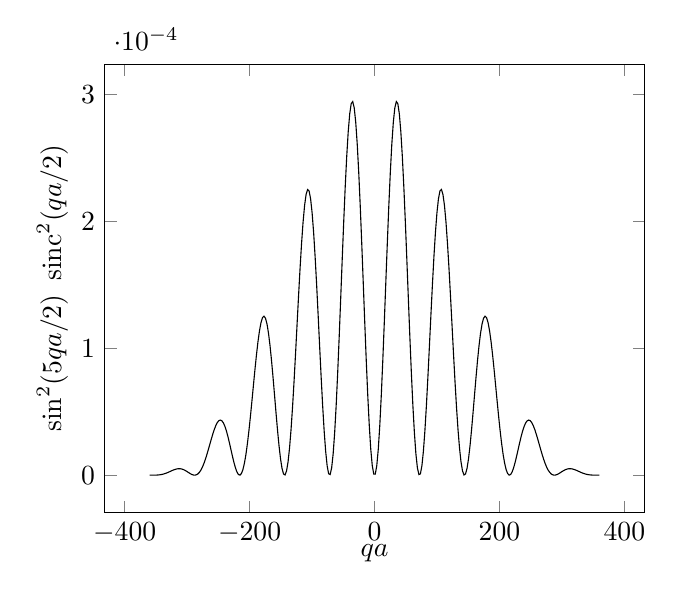
\begin{tikzpicture} 
    \begin{axis}[
    x label style={at={(axis description cs:0.5,-0.05)},anchor=north},
    y label style={at={(axis description cs:-0.05,.5)},anchor=south},
    ylabel={$\sin^2(5qa/2)~ \sinc^2(qa/2)$},
    xlabel={$qa$}]
      \addplot [domain = -360:360, samples = 300] ({\x},{(sin(\x/2)/(\x/2))^2*(sin(5*\x/2))^2});
 \end{axis}
\end{tikzpicture}
\end{center}
\end{enumerate}
\end{ans}
\newpage
\begin{qns}[Michelson Interferometry]\leavevmode
\begin{enumerate}[label=(\alph*)]
\item Explain what is meant by the terms ‘division of amplitude’ and ‘division of wavefront’ in the context of interferometry.\hfill\textbf{[2]}
\item Draw a labelled diagram of a Michelson interferometer.\hfill\textbf{[3]}
\item For monochromatic light entering the Michelson interferometer, assuming an equal intensity of the interfering beams of $I_0/2$, show that the intensity of the resulting fringe pattern varies as
$$I(x)=I_0(1+\text{Re}[e^{ikx}])$$
where $k$ is the wavenumber and $x$ is the difference in paths travelled by the two beams. Draw a graph of the intensity variation of the fringe pattern, annotating the positions of the minima.\hfill\textbf{[5]}
\item The light entering the Michelson interferometer is now replaced with the light from a sodium lamp. Sketch how the output intensity of the fringe pattern changes as a function of mirror displacement for the sodium D line, using the fact that the D line is actually a doublet centered at 589.3 nm with $\Delta\lambda$=0.6 nm. Annotate your sketch with appropriate values for the periodicities.\hfill\textbf{[6]}
\item A broadband light source is now used. Explain how this configuration can be used to perform Fourier transform spectroscopy. For a wavelength of 500 nm, what value of mirror displacement is needed to achieve a spectral resolution of 0.01 nm?\hfill\textbf{[4]}
\end{enumerate}
\end{qns}
\begin{ans}\leavevmode
\begin{enumerate}[label=(\alph*)]
\item Division of amplitude: A Michelson interferometer uses a semi-silvered mirror mounted on a piece of glass to split a single beam into two.\\[5pt]
Division of wavefront: an interferometer combines two or more different light beams, while a diffraction grating uses different parts of the same wavefront to combine them to form fringes.
\item The beam-splitter splits the incident beam with components travel along different paths, and recombine at the same beam-splitter. One path is kept fixed (reference path) and the other path is varied with a movable mirror on a precision stage. A fringe pattern is obtained as a function of mirror position. $d$ is the distance from the beam splitter to the fixed mirror, and $\frac{x}{2}$ is the excess distance to the movable mirror such that the light travels an extra distance of $2\frac{x}{2}=x$ to and fro.
\begin{figure}[H]
    \centering
    \includegraphics[width=\linewidth]{mmi.PNG}
    \caption{Michelson Interferometer Setup}
    \label{fig:my_label}
\end{figure}
\item $\psi_0$ is the amplitude entering the beam splitter, $\psi_1=\frac{\psi_0}{\sqrt{2}}e^{2ikd}$ is the amplitude for the light bouncing off the fixed mirror, $\psi_2=\frac{\psi_0}{\sqrt{2}}e^{2ikd}e^{ikx}$ is the amplitude for the light bouncing off the movable mirror. After recombination,
$$I=(\text{Re}[\psi_1+\psi_2])^2=|\psi_1|^2+|\psi_2|^2+2\text{Re}[\psi_1\psi_2^*]=\frac{I_0}{2}+\frac{I_0}{2}+2\frac{I_0}{2}\text{Re}[e^{ikx}]=2I_0\cos^2(kx/2)$$
The sketch of $\frac{I}{I_0}$ against $x$ will be a $\cos^2$ graph with distance between consecutive minima being $\frac{2\pi}{k}=\lambda$. The minimas (zeroes) occur at $x=\frac{2n+1}{2}\lambda$.
\item With two different frequencies, the time-averaged for the mixing terms will be zero. We can simply add the intensities. Assuming the doublet has equal power in each wavelength $\lambda_{1,2}=\lambda_0\pm\frac{\Delta\lambda}{2}$, then
$$I=I_0(1+\cos k_x)+I_0(1+\cos k_2x)=2I_0+2I_0\cos\frac{k_1+k_2}{2}x\cos\frac{k_1-k_2}{2}x$$
Now, $\frac{k_1\pm k_2}{2}=\pi\frac{\lambda_2\pm\lambda_1}{\lambda_1\lambda_2}$, which gives either $-\frac{\Delta\lambda}{\lambda_0^2}\pi$ and $\frac{\pi 2\lambda_0}{\lambda_0^2}$. Hence,
$$I=2I_0\bigg(1+\cos\frac{2\pi x}{\lambda_0}\cos\frac{\pi\Delta\lambda}{\lambda_0^2}x\bigg)$$
This is a slow cosine envelope ($\cos\frac{\pi\Delta\lambda}{\lambda_0^2}x$ with wavelength $\frac{\lambda_0^2}{\Delta\lambda}$) modulating a fast cosine ($\cos\frac{2\pi x}{\lambda_0}$ with wavelength $\lambda_0$). The number of fast oscillations per slow oscillation is $\frac{2\pi}{\lambda_0}\frac{1}{\pi\Delta\lambda/\lambda_0^2}=\frac{2\lambda_0}{\Delta\lambda}=\frac{2(589.3\times10^{-9}}{0.6\times10^{-9}}=1964$.
\begin{figure}[H]
    \centering
    \includegraphics[scale=0.95]{2018P2B8ii.PNG}
    \caption{Beating phenomena. Graph not drawn to scale.}
\end{figure}
Assuming Sodium D lines have no intrinsic line widths, which will further modulate the waveform with a Gaussian, reducing the visibility of the fringes, where visibility (fringe contrast) is $\frac{I_{max}-I_{min}}{I_{max}+I_{min}}$.
\item If we denote the intensity in the range $k$ to $k+dk$ as $2S(k)dk$, where strictly this is only defined for $k\geq0$. We can then extend $S(k)$ such that $S(-k)=S^*(k)$.
$$I(x)=\int_0^\infty 2S(k)(1+\text{Re}[e^{ikx}])dk=\int_{-\infty}^\infty S(k)(1+\text{Re}[e^{ikx}])dk\implies S(k)=\frac{1}{2\pi}\int_{-\infty}^\infty[I(x)-I_0]e^{-ikx}dx$$
The mirrors can only be moved to create a finite path difference $x_{max}$. This effectively further multiplies $I(x)$ by $\text{rect}(x/2x_{max})$. In $k$-space, we convolve it with a sinc whose first zero is at $\frac{2\pi}{x_{max}}$. The resolving power is given as $\frac{\Delta\lambda}{\lambda}=\frac{\lambda}{x_{max}}\implies x_{max}=\frac{\lambda^2}{\Delta\lambda}=\frac{(500\times10^{-9})^2}{0.01\times10^{-9}}=2.5$ cm. 
\end{enumerate}
\end{ans}
\newpage
\begin{qns}[Impedance]
A light string, of mass $\rho$ per unit length, is stretched under tension $T$ along the $x$ axis.
\begin{enumerate}[label=(\alph*)]
\item Show that the motion arising from small transverse displacements $\Psi(x,t)$ can be described by the wave equation\hfill\textbf{[5]}
$$\frac{\partial^2\Psi}{\partial t^2}=v^2\frac{\partial^2\Psi}{\partial x^2}$$
\item Give a general definition of the term wave impedance and derive the wave impedance of the string.\hfill\textbf{[2]}
\item The mean power required to drive an oscillator can be expressed by \hfill\textbf{[3]}
$$\langle P\rangle=\frac{1}{2}\text{Re}[\mathbf{F}\mathbf{u^*}]$$
where $\mathbf{F}$ is the force applied and $\mathbf{u}$ is the velocity, both described in complex notation. What is the mean power carried along the string when it is driven by force $\mathbf{F}$ at velocity $\mathbf{u}$?
\item State the conditions that must be satisfied by $\Psi$ and $\partial\Psi/\partial x$ at any point on the string.\hfill\textbf{[2]}
\item The wave encounters a discontinuity in mass density on the string. Explain the following observations by considering the mass densities on either side of the discontinuity $\rho_1$ and $\rho_2$:

\hfill\textbf{[8]}
\begin{enumerate}[label=(\roman*)]
    \item A phase change is observed in the reflected wave at the boundary.
    \item The wave amplitude and energy is entirely reflected at the boundary.
    \item No reflection is observed at the boundary.
\end{enumerate}
\end{enumerate}
\end{qns}
\begin{ans}\leavevmode
\begin{enumerate}[label=(\alph*)]
\item The force on a string element is
$$\rho\Delta x\frac{\partial^2\psi}{\partial t^2}=T\bigg(\frac{\partial\psi}{\partial x}
(x+\Delta x)-\frac{\partial\psi}{\partial x}(x)\bigg]\approx T\frac{\partial^2\psi}{\partial x^2}\Delta x$$
where we obtained a wave equation with speed $v=\sqrt{T/\rho}$.
\item The impedance $Z$ is the ratio of driving force to the velocity response.
$$Z=\frac{-T\frac{\partial\psi}{\partial x}}{\frac{\partial\psi}{\partial t}}=\frac{-T(-ik\psi)}{i\omega\psi}=\frac{T}{v}=\sqrt{T\rho}$$
\item For $\mathbf{F}=\mathbf{F_0}e^{i\omega t}$, then $\mathbf{F}=Z\mathbf{u}$. We have the time-averaged power to be $\langle P\rangle=\frac{1}{2}|F_0|^2\text{Re}[Z]=\frac{1}{2}|\mathbf{u}|^2\text{Re}[Z^{-1}]$. But $Z$ is real, so $\langle P\rangle=\frac{|u|^2}{2Z}$.
\item $\psi$ and $T\frac{\partial\psi}{\partial x}$ are continuous. Since $T$ is continuous, $\frac{\partial\psi}{\partial x}$ is continuous.
\item We guess an ansatz $\psi=Ae^{i(\omega t-kx)}+Are^{i(\Omega t+kx)}$ for $x<0$ and $\psi=\tau Ae^{i(\omega t-qx)}$ for $x>0$, where $\Omega$ and $q$ are angular frequency and wavevector respectively in $x>0$. $\psi$ is continuous $\forall t$, so $(1+r)e^{i\omega t}=\tau e^{i\Omega t}\implies\Omega=\omega$ and $1+r=\tau$. $\frac{\partial\psi}{\partial x}$ is continuous $\forall t$, so $-ik(1-r)=-iq\tau$. We thus have 
$$1-r=\frac{q}{k}\tau=\frac{q}{\omega}\frac{\omega}{k}(1+r)=\frac{v_1}{v_2}(1+r)=\frac{Z_2}{Z_1}(1+r)\implies r=\frac{Z_1-Z_2}{Z_1+Z_2}=\frac{\sqrt{\rho_1}-\sqrt{\rho_2}}{\sqrt{\rho_1}+\sqrt{\rho_2}}$$
\begin{enumerate}[label=(\roman*)]
    \item $r<0\implies \rho_2>\rho_1$.
    \item $r=\pm 1\implies$ for finite $\rho_1$, $\rho_2=0$ or $\infty$ for $r=+1$ and $-1$ respectively.
    \item $r=0\implies\rho_1=\rho_2$.
\end{enumerate}
\end{enumerate}
\end{ans}
\newpage
\subsubsection{Section C}
\begin{qns}[Heat Capacity]\leavevmode
\begin{enumerate}[label=(\alph*)]
\item  State the main assumptions of the free electron model.\hfill\textbf{[3]}
\item Derive an expression for the density of states and the Fermi energy for a 3D electron gas within the free electron model.\hfill\textbf{[6]}
\item Sketch the form of the Fermi Dirac distribution as the temperature is gradually raised from a starting point of 0K. Explain any assumptions you have made.\hfill\textbf{[3]}
\item Explain how these results can be used to argue that the electronic heat capacity can be approximated as $\frac{9}{2}Nk_B\frac{T}{T_F}$.\hfill\textbf{[4]}
\item Calculate the electronic heat capacity of sodium with density 0.97 g cm$^{-3}$ and relative atomic mass 23 at 300K given that the Fermi energy can be taken to be 3.24 eV. Comment on the discrepancy between your calculated value and the measured heat capacity of sodium at 300K, which is approximately 28 J Mol$^{-1}$ K$^{-1}$.\hfill\textbf{[4]}
\end{enumerate}
\end{qns}
\begin{ans}\leavevmode
\begin{enumerate}[label=(\alph*)]
\item FEM neglects the effects of the periodic lattice potential by averaging over the interactions with all the atomic cores and the outer electrons, to get a constant uniform potential.
\item Impose periodic boundary conditions along the $x$ directions $k_xL_x=2n\pi$. Similarly, $k_y=\frac{2\pi}{L_y}n_y$ and $k_z=\frac{2\pi}{L_z}n_z$, for $n_x,n_y,n_z\in\mathbb{Z}^+\cup\{0\}$. Each state occupies a region of volume 
$$\Delta k_x\Delta k_y\Delta k_z=\frac{(2\pi)^3}{L_xL_yL_z}=\frac{(2\pi)^3}{V}$$
The density of states $g(E)$ is such that $g(E)dE$ gives the number of states with energy $E$ to $E+dE$. In momentum representation, we have
$$g(p)dp=\frac{4\pi p^2dp}{2(2\pi\hbar)^3/V}$$
where we account for the spin degeneracy factor of 2, and the volume of the spherical shell is $4\pi p^2dp$. But $p^2=2mE$, so
$$g(E)dE=2V\frac{4\pi}{(2\hbar\pi)^3}2mEd\sqrt{2mE}=\frac{V}{\hbar^3\pi^2}2mE\frac{1}{2}\sqrt{\frac{2m}{E}}dE=\frac{V\sqrt{2m^3}}{\pi^2\hbar^3}\sqrt{E}dE$$
The density of states is thus $g(E)=\frac{V\sqrt{2m^3}}{\pi^2\hbar^3}\sqrt{E}$. The number of states is
$$N=\int_0^{E_F}g(E)dE=\frac{V\sqrt{2m^3}}{\hbar^3\pi^2}[2E^{3/2}/3]_0^{E_F}=\frac{2V}{3\hbar^3\pi^2}\sqrt{2m^3E_F^3}$$
which gives the Fermi energy to be $E_F=\frac{\hbar^2}{2m}(3\pi^2n)^{3/2}$ with $n$ being the number density.
\item The Fermi-Dirac distribution gives the probability of a state of energy $E$ being occupied:
$$p(E)=\frac{1}{e^{\beta(E-\mu(T))}+1}$$
where $\beta=\frac{1}{k_BT}$ and $\mu(T)$ is the chemical potential at temperature $T$. Below is a plot with the red curve at a lower temperature. At $T=0$, $p(E)=H(E-\mu(0))$ is a step function, where $\mu(T=0)$ is defined to be the Fermi energy $E_F$. With a constant particle number, $\mu(T)\approx E_F$ for sufficiently small temperatures.
\begin{center}
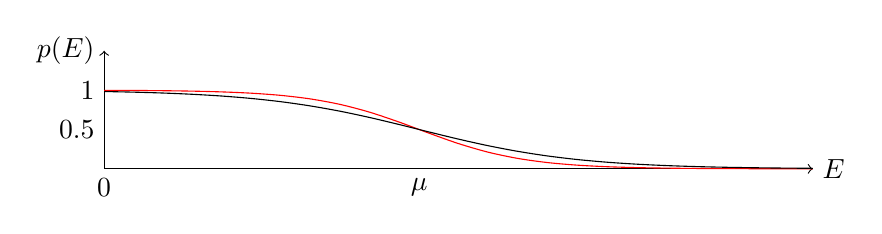
\begin{tikzpicture}
      \draw[->] (0,0) -- (9,0) node[right] {$E$};
      \draw[->] (0,0) -- (0,1.5) node[left] {$p(E)$};
      \draw[domain=0:9,smooth,variable=\x,red] plot ({\x},{1/(exp(1.5*(\x-4))+1)});
      \draw[domain=0:9,smooth,variable=\x,black] plot ({\x},{1/(exp((\x-4))+1)});
      \draw (0,0) node[below]{0};
      \draw (0,0.5) node[left]{$0.5$};
      \draw (4,0) node[below]{$\mu$};
      \draw (0,1) node[left]{$1$};
\end{tikzpicture}
\end{center}
\item Since electrons are fermions, they obey the Pauli Exclusion principle - no two fermions will occupy the same quantum state. Hence, the fermions will fill the states from the lowest energy upwards. The state with the highest possible energy defines the Fermi level. Only electrons with energy within $k_BT$ of $E_F$ may be thermally activated at $T>0$. Each such electron will have an energy of $\frac{3}{2}k_BT$ and so the total thermal energy associated with these electrons is
$$U=\frac{3}{2}k_BTg(E_F)k_BT=\frac{9k_B^2T^2}{4k_BT_F}N$$
where the density of state at Fermi energy is $g(E_F)=\frac{3N}{2E_F}=\frac{3N}{2k_BT_F}$ where $T_F$ is the characteristic temperature of the Fermi energy. The heat capacity is 
$$C=\frac{\partial U}{\partial T}=\frac{9}{2}Nk_BT\frac{T}{T_F}$$
\item Since sodium's valency is 1, each sodium atom contributes an electron. The molar heat capacity at constant volume is
$$C_V=\frac{9}{2}\frac{300}{3.24(1.6\times10^{-19})}(1.38\times10^{-23})^2(6.02\times10^{23})=1.0\times10^{-3}J\text{ mol}^{-1}K^{-1}$$
This difference is due to the phononic contribution to the heat capacity.
\end{enumerate}
\end{ans}
\begin{qns}[Transport]\leavevmode
\begin{enumerate}[label=(\alph*)]
\item Explain why the concept of effective mass is useful. Show that the effective mass of an electron can be written as:\hfill\textbf{[6]}
$$m^*=\hbar^2\bigg(\frac{d^2\epsilon}{dk^2}\bigg)^{-1}$$
\item By considering the motion of an electron in an electric field, show that the electrical conductivity, $\sigma$, can be written in terms of the number of electrons per volume $n$, their charge $e$ and the electron mobility $\mu$:\hfill\textbf{[4]}
$$\sigma=ne\mu$$
\item Calculate the drift velocity for copper with density 8.94 g cm$^{-3}$ and relative atomic mass 63.5 in a 3 mm wire at a current of 13 A. Find an approximate value for the distance travelled by an electron during a 50 Hz mains cycle. Assume that copper has one electron per atom available for conduction.\hfill\textbf{[5]}
\item Sketch a diagram showing the temperature dependence of electrical resistivity, explaining the different regimes present. Referring to the diagram, suggest a reason why pure iron generally has a lower electrical resistivity than mild steel which is approximately 99.75\% iron and 0.25\% carbon.\hfill\textbf{[5]}
\end{enumerate}
\end{qns}
\newpage
\begin{ans}\leavevmode
\begin{enumerate}[label=(\alph*)]
\item The effective mass accounts for the influence of the periodic lattice potential on the electron's motion. With this, we can continue to use semi-classical equations of motion to study electron dynamics in a solid. The `kinetic energy' is a function of $k$ and encapsulates the effective mass.
$$\epsilon(k)=\frac{\hbar^2k^2}{2m^*}\implies m^*=\hbar^2\bigg(\frac{d^2\epsilon}{dk^2}\bigg)^{-1}$$
\item We define the electron mobility to be a ratio of the electron's drift velocity in the presence of an external electric field to the magnitude of this field.
$$\mu:=\frac{v_d}{E}$$
But the current density of $n$ electrons per unit volume is
$$\mathbf{J}=ne\mathbf{v_d}=ne\mu\mathbf{E}\implies\sigma=ne\mu$$
where $\sigma$ is the conductivity.
\item The drift velocity is
$$v_d=\mu E=\frac{\sigma}{ne}\frac{J}{\sigma}=\frac{1}{ne}\frac{I}{\pi r^2}=\frac{13(63.5)1.66\times10^{-27}}{\pi(3\times10^{-3})^2(1.6\times10^{-19}(8.94\times10^3)}=3.4\times10^{-5}m/s$$
For a 50 Hz AC field, the displacement is $x=x_0+A\cos(100\pi t)$ with amplitude $A=\frac{v_d}{2\pi f}$. The particle will move a total distance of 
$$2A=\frac{v_d}{\pi f}=\frac{3.388\times10^{-5}}{\pi 50}=2.157\times10^{-7}m$$
\item At low temperatures, the scattering rate is determined by geometric factors such as lattice defects and impurities. At high temperatures, the scattering off phonons becomes more relevant. The mean time between collisions $\tau$ is
$$\frac{1}{\tau}=\frac{1}{\tau_{geom}}+\frac{1}{\tau_{phon}}$$
In equilibrium, the acceleration of the electrons is zero as that due to the electric field balance with that due to geometric scattering.
$$0=\frac{m^*v_d}{\tau}-eE\implies\tau=\frac{m^*v_d}{eE}=\frac{m^*\mu}{e}$$
where $\tau$ is the scattering time. The resistivity is thus
$$\frac{1}{\sigma}=\frac{1}{ne\mu}=\frac{m^*}{ne\tau}$$
At low temperatures, $\frac{1}{\sigma}\approx\frac{1}{\sigma_{geo}}$ a constant. As temperature increase, phonon-phonon scattering dominates and $\frac{1}{\sigma}$ show a linear dependence with temperature. As for mild steel, the presence of carbon impurities increases $1/\tau_{geo}$ due to scattering off such impurities. This is assuming similar grain size and dislocation density. If this is not true, there will be a temperature-independent offset determined by Matthiessen's rule.
\end{enumerate}
\end{ans}
\newpage
\subsubsection{Section D}
\begin{qns}[CMP Essay]
Write an essay on doping in semiconductors including a brief discussion of how this gives rise to the concept of a P-N junction.\hfill\textbf{[20]}
\end{qns}
\begin{ans}
Adding dopants that gives more (fewer) electrons than the substrate itself creates an n-type (a p-type) semiconductor. At non-zero temperatures, all these states are ionized, increasing the conductance of the material. For the n-type (p-type), the vast majority of the charge carriers are ionized electrons (holes left behind when electrons from the filled band were excited into the dopant hole state). In the absence of impurities, the Fermi energy ($\mu(T=0)$) is in the middle of the band gap. When the donor (acceptor) impurities are added, at zero temperature, impurity states near the top (bottom) of the bandgap are filled (empty). The Fermi energy is moved up to the top (down to the bottom) of the band gap.\\[5pt]
Although the n-doped system has free negatively charged electrons and the p-doped system has free positively charged holes, both systems are overall electrically neutral since charged ions compensate for the charges of the mobile charge carriers. When the two doped semiconductors are brought into contact, the electrons in the conduction band will fall into the valence band, filling the empty hole states, thus pair-annihilating both the electron and the hole. This amounts to a gain in energy of $E_{gap}$ per pair annihilated.\\[5pt]
After this process of electrons falling into holes and annihilating occurs there will be a region near the interface where there are no free carriers at all. This is the depletion region, which is electrically charged (since there are charged ions but no carriers to neutralize them). Hence, there is a net electric field pointing from the positively charged to the negatively charged ions.\\[5pt]
We now imagine moving an additional electron across the depletion region in order to annihilate another hole. While the annihilation process gives a gain in energy of $E_{gap}$, the process of moving the electron across the depletion region costs an energy of $-e\Delta\phi$, where $\phi$ is the electrostatic potential. When the depletion region is sufficiently large, it becomes no longer favorable for further electrons and holes to annihilate. \\[5pt]
Rectification: allow current to flow through the junction easily in one direction, but not the other. There are 4 processes that can create current:
\begin{enumerate}
    \item Electrons may be thermally excited into the conduction band. Some of these electrons will flow down the slope to the left.
    \item Holes may be thermally excited down into the valence band and will flow up the slope to the right. 
    \item Electrons in the conduction band on the left will be thermally activated to climb up the potential slope in the depletion layer and will annihilate with holes once they arrive at the p-doped side. 
    \item Holes in the valence band on the right may be thermally activated to climb down the potential slope towards the n-doped side where they annihilate with electrons.
\end{enumerate}
The contribution by processes 1 and 2 to the current is directly proportional to $e^{-E_{gap}/k_BT}$. Voltage bias will not change the number of excited carriers, hence current independent of voltage. The contribution by processes 3 and 4 to the current is directly proportional to $e^{-E_{gap}/k_BT}$ in the absence of an applied voltage, and $e^{-(E_{gap}+eV)/k_BT}$ in the presence of an applied voltage. The total current flow will be the sum and hence
$$I=J_s(T)(e^{-eV/k_BT}-1)$$
where $J_s$ is directly proportional to $e^{-E_{gap}/k_BT}$ is known as the saturation current. This is the diode equation. Current flows easily in one direction, i.e. forward biased, but flows poorly in the opposite direction, i.e. reverse biased.
\begin{figure}[H]
    \centering
    \includegraphics[width=\linewidth]{pnjunction.PNG}
    \caption{Description of PN Junction. The drop in band energy is precisely compensated by the change in electrostatic potential. Image credit: CMP Notes by Cavendish.}
\end{figure}
\begin{figure}[H]
    \centering
    \includegraphics[width=\linewidth]{biasedPN.PNG}
    \caption{Band diagram of a biased p-n junction. The four processes that can create current are labelled. In the absence of applied voltage, the net current is zero. When voltage is applied, current flows easily for $eV<0$ and not easily with $eV>0$. Image from S.H. Simon: The Oxford Solid State Basics. }
\end{figure}
\end{ans}
\newpage
\begin{qns}[OWO Short Notes]
Write brief notes on two of the following:\hfill\textbf{[20]}
\begin{itemize}
    \item convolution and the convolution theorem as applied to the interpretation of Fraunhofer diffraction patterns;
    \item thin film interference;
    \item dispersion, group velocity and phase velocity.
\end{itemize}
\end{qns}
\begin{ans}\leavevmode
\subsubsection*{Convolution and the convolution theorem as applied to the interpretation of Fraunhofer diffraction patterns:}
Convolution theorem states that the Fourier transform of a product of two functions is the convolution of the Fourier transforms of the individual functions.
$$f(y)*g(y)=\int_{-\infty}^\infty f(u)g(y-u)du$$
Consider the diffraction pattern in a plane at a distance $L$ from the aperture. We denote the coordinates of point P in this plane by $(x_0,y_0)$ and further assume P to be close to the axis. Assume that the source S is a large distance behind the aperture, and the aperture is illuminated with a plane wave at normal incidence. The wave amplitude at P is directly proportional to the Fraunhofer integral
$$\int_\Sigma\psi_\Sigma h(x,y)e^{-ik(x_0x+y_0y)/R}dxdy$$
Moreover, the condition for Fraunhofer diffraction is $\frac{k(x^2+y^2)}{2R}<<\pi$. The Fraunhofer integral is a simplified version of the general Fresnel-Kirchhoff diffraction integral, where the approximation $x_0/L,y_0/L<<1$ gives a linear phase variation (as seen from any given point on the aperture plane). We see that the Fraunhofer integral is actually a Fourier transform of the aperture function $h(x,y)$. This Fourier transform relates real space variables $x,y$ to the conjugate ones $q=k\sin\theta$ and $p=k\sin\xi$. For some one-dimensional simple apertures, we can easily obtain the analytic descriptions of the Fraunhofer diffraction patterns:
$$\mathcal{F}[\sum_{m=0}^\infty\delta(y-mD)]=\sum_{m=0}^\infty\delta(q-m\frac{2\pi}{D})$$
$$\mathcal{F}[\text{rect}(y/a)]=a\sinc(qa/2)$$
These two functions are key building blocks in deriving the diffraction pattern of more complicated aperture functions, as illustrated below.
\begin{figure}[H]
    \centering
    \includegraphics[scale=0.75]{convolution.PNG}
\end{figure}
A more complicated example would be an array of 6 very small, identical circles arranged in a regular hexagon whose sides are of length $a$, with 2 of the circles located at $(x_i, y_i) = (0,\pm 2a)$. The aperture function is
$$h(x,y)=\bigg[\sum_{i=1}^6\delta(x-x_i)\delta(y-y_i)\bigg]*o(x,y)$$
where $(x_i,y_i)=(0,\pm2a)$, $(\sqrt{3}a,\pm a)$, $(-\sqrt{3}a,\pm a)$ for the hexagonal geometry and $o(x,y)$ is the aperture function for a single hole. Taking the Fourier transform and invoke the convolution theorem, we have
$$F(p,q)=\int h(x,y)e^{i(px+qy)}dxdy=O(p,q)\bigg[(e^{i2aq}+e^{-i2aq})+e^{-\sqrt{3}pai}(e^{iaq}+e^{-iaq})+e^{\sqrt{3}pai}(e^{iaq}+e^{-iaq})\bigg]$$
where $O(p,q)=\mathcal{F}[o(x,y)]$. The intensity is thus directly proportional to $(2\cos(2qa)+4\cos(\sqrt{3}pa)\cos(qa))^2$.
\newpage
\subsubsection*{Thin film interference:}
Consider light incident (in medium 1) at an interface separating two media of refractive indices $n_1$ and $n_2$ where $n_2>n_1$, and the thickness of medium 2 is $t$. Since $n_2>n_1$, the ray reflected from this interface acquires a phase change of $\pi$ (otherwise, if $n_2<n_1$, no such phase change occurs). We assume the medium below medium 2 has a smaller refractive index. Let $n_1=1$ and $n_2=n$, the path difference is
$$n\bigg(\frac{t}{\cos\theta}+\frac{t}{\cos\theta}-(2t\tan\theta)\sin\theta_i\bigg)=\frac{2nt}{\cos\theta}-\frac{2nt\sin^2\theta}{\cos\theta}=2nt\cos\theta$$
where we used Snell's Law $\sin\theta_i=n\sin\theta$. The phase difference $\delta$ will be the path difference multiplied by $\frac{2\pi}{\lambda}$, plus the additional $\pi$ phase. If $\delta$ is a integer multiple of $2\pi$, i.e. $2nt\cos\theta\frac{2\pi}{\lambda}=(2m+1)\pi$, the beams are in phase and bright fringes are observed. Conversely, $2nt\cos\theta\frac{2\pi}{\lambda}=2m\pi$, the beams are in anti-phase and dark fringes are observed. \\[5pt]
If the two interfering beams differ in strength, the fringes are still present with the same period, but are less distinct (contrast) since they sit on top of a constant background. With a beamsplitter, lens and extended source, circular fringes of equal inclination $\theta_i$, known as Haidinger fringes, may be observed.\\[5pt]
For films of non-uniform thickness, the corresponding interference fringes are known as fringes of equal thickness $t$. For a wedge, the resulting interference fringes are localized near and are almost parallel to the thin end of the wedge. For soap films, when illuminated with white light, each wavelength component produces its own set of fringes with a different period. The superposition of these fringes leads to a complex pattern of colours across the film.
\begin{figure}[H]
\centering
\includegraphics[width=\linewidth]{thinfilm.PNG}
\end{figure}
\newpage
\subsubsection*{Dispersion, group velocity and phase velocity:}
Dispersive waves have the following dispersion relation: $\omega(k)$ that is not a constant, and is a function of $k$. Different wavelengths travel at different phase speeds.\\[5pt]
The phase velocity of a wave is the rate at which the phase of the wave propagates in space. This is the velocity at which the phase of any one frequency component of the wave travels. $v_p=\frac{\omega(k)}{k}$. The group velocity of a wave is the velocity with which the overall envelope shape of the wave's amplitudes—known as the modulation or envelope of the wave—propagates through space.\\[5pt]
A wavepacket consists of a superposition of waves with a range of frequencies. In a dispersive medium, the individual components will travel at different speed. The shape of the wavepacket changes with propagation, and hence the wavepacket will spread out and eventually disappear. The wavepacket transfers energy at a speed equal to group velocity. Consider a wavepacket consisting of a carrier wave with wavenumber $k_0$, multiplied by an envelope $f(x)$, such that it has significant amplitude only over a small wavenumber range $\Delta k$, where $\Delta k<<k_0$. Then, its time-independent form will be
$$\psi(x,0)=\text{Re}[f(x)e^{ik_0x}]$$
The corresponding time-dependent form is
$$\psi(x,t)=\text{Re}[f(x-v_gt)e^{ik_0(x-v_pt)}]$$
where $v_p$ and $v_g$ are phase and group velocities respectively.\\[5pt]
Rewriting $\psi(x,0)$ as $\text{Re}[(\int_{-\infty}^\infty F(k_1)e^{ik_1x}dk_1)e^{ik_0x}]$ such that each sinusoid with wavenumber $k_0+k_1$ will propagate at its own phase velocity and that $F(k_1)$ is the Fourier transform of $f(x)$. At $t>0$, we have
$$\psi(x,t)=\text{Re}\bigg[\int_{-\infty}^\infty F(k_1)e^{i(k_0+k_1)x-(\omega_0+\omega_1)t}dk_1\bigg]$$
where $\omega_0=\omega(k_0)$ and $\omega_0+\omega_1=\omega(k_0+k_1)$. Given the assumption where $F(k_1)$ is non-zero over a small wavenumber range $\pm\Delta k$, where $\Delta k<<k_0$. Expanding $\omega$ about $k_0$,
$$\omega\approx\omega_0+\frac{\partial\omega}{\partial k}\bigg|_{k=k_0}k_1+\frac{1}{2}\frac{\partial^2\omega}{\partial k^2}\bigg|_{k=k_0}k_1^2$$
where $v_g=\frac{\partial\omega}{\partial k}(k=k_0)$ and $v_p=\omega_0/k_0$. Finally,
$$\psi(x,t)=\text{Re}\bigg[\int_{-\infty}^\infty F(k_1)e^{-ik_1v_gt}e^{ik_1x}dk_1e^{i(k_0x-\omega_0t)}\bigg]=\text{Re}[f(x)*\delta(x-v_gt)e^{i(k_0x-\omega_0t)}]$$
and then as desired. Essentially, the modulating envelope propagates at speed $v_g$. The group velocity $v_g$ may be expressed as the phase velocity $v_p$ like the following:
$$v_g=\frac{d\omega}{d k}=\frac{d}{dk}(kv_p)=v_p+k\frac{dv_p}{dk}=v_p-\lambda\frac{dv_p}{d\lambda}$$
When $v_g>v_p$ or $\frac{dv_p}{d\lambda}<0$, the carrier wave move backwards through the envelope. $v_p$ decrease with $\lambda$ so long $\lambda$ appear at the rear of the packet, i.e. anomalous dispersion. We hear this as a down-chirp.\\[5pt]
Conversely, when $v_g<v_p$ or $\frac{dv_p}{d\lambda}>0$, the carrier wave move forwards through the envelope. $v_p$ increases with $\lambda$ so long $\lambda$ appear at the front of the packet, i.e. normal dispersion. We hear this as an up-chirp.\\[5pt]
Electrical conductor is anomalously dispersive to electromagnetic waves whilst a dielectric is normally dispersive except at the natural resonant frequencies of its atoms.
\end{ans}
\newpage
\section{2019}
\subsection{Paper 1}
\subsubsection{Section A}
\begin{qns}[1D Potential]
An electron is confined to a cube of edge 1 nm. Use the uncertainty principle to estimate the minimum kinetic energy of the electron.\hfill\textbf{[4]}
\end{qns}
\begin{ans}
Treat it as infinite cubic potential well that is stationary, such that $\langle p_i\rangle=0$ $\forall i=x,y,z$. Then, it follows that $\langle\Delta p_x^2\rangle=\langle p_x^2\rangle$. By the Uncertainty principle, $\Delta p_x\Delta x\geq\frac{\hbar}{2}$, then the kinetic energy is
$$K=\frac{3\Delta p_x^2}{2m_e}\geq\frac{3}{2m_e}\frac{\hbar^2}{(2\Delta x)^2}=\frac{3(6.626\times10^{-34}/(2\pi))^2}{2(1.6\times10^{-19})(2\times10^{-9})^2}=0.03eV$$
\end{ans}
\begin{qns}[Angular Momentum]
Write down the kinetic energy of a rotating object in terms of its angular  momentum $L$ and moment of inertia $I$. Hence find the energies, in eV, of the three lowest energy levels for an object with $I$ = 10$^{-47}$ kg m$^2$.\hfill\textbf{[4]}
\end{qns}
\begin{ans}
The energy of a classical rigid rotor is $\frac{L^2}{2I}$ and so the Hamiltonian of the quantum version is $\frac{\hat{L}^2}{2I}$, with energy eigenvalues $E_l=\frac{\hbar^2}{2I}l(l+1)$. $E_{l=0}=0$ eV, $E_{l=1}=\frac{\hbar^2}{I}=\frac{(6.626\times10^{34}/2\pi)^2}{10^{-47}}=6.95$ meV and $E_{l=2}=\frac{2\times 3}{2}E_1=0.02$ eV.
\end{ans}
\begin{qns}[1D Potential]
An electron of kinetic energy 8 eV and zero potential energy approaches a square potential barrier of height 10 eV and width 1 nm. Estimate the probability that the electron will tunnel through the barrier.\hfill\textbf{[4]}
\end{qns}
\begin{ans}
The tunnelling probability is
$$e^{-2ka}=\exp\bigg(-2a\frac{\sqrt{2m|E-U|}}{\hbar}\bigg)=\exp\bigg(-2(10^{-9})\frac{\sqrt{2(9.11\times10^{-31}|8-10|(1.6\times10^{-19})}}{6.626\times10^{34}/2\pi}\bigg)=5.1\times10^{-7}$$
\end{ans}
\begin{qns}[Noise]
The current through a resistor $R = 1$ G$\Omega$ at an applied voltage $V = 1$ mV is measured for short periods lasting 1 s. Calculate the expected current and estimate how many measurements are necessary to determine the average current to a precision of $\leq 10^{-5}$.\hfill\textbf{[4]}
\end{qns}
\begin{ans}
The number of electrons is $N=\frac{It}{e}$. The error in current is $\Delta I=\frac{e}{t}\Delta N$. Shot noise is an example of Poisson distribution such that $\Delta N=\sqrt{N}$. Hence, after $n$ number of measurements, the expected current is
$$\Delta I_{mean}=\frac{\Delta I}{\sqrt{n}}=\frac{1}{\sqrt{n}}\sqrt{\frac{Ie}{t}}$$
For $\frac{\Delta I_{mean}}{I}\leq 10^{-5}$, where $I=\frac{V}{R}$, we require
$$n\geq (10^{-5})^{-2}\bigg(\frac{\Delta I}{I}\bigg)^2=(10^{-5})^{-2}\frac{1}{I^2}\frac{Ie}{t}=(10^{-5})^{-2}\frac{eR}{tV}=1600$$
\end{ans}
\begin{qns}[Error Analysis]
The numerical aperture $N$ of a microscope objective is given by $N = n \sin\alpha$, where $n$ is the refractive index of the immersion fluid and $\alpha$ the opening angle. $n$ is known to be $1.35\pm0.075$ while $\alpha$ is known to be around 60\degree. To what precision do you need to determine $\alpha$ so that $N$ is known to within 6\%.\hfill\textbf{[4]}
\end{qns}
\begin{ans}
We have $N=n\sin\alpha=1.35\sin(60\degree)=1.169$. Assuming the errors are Gaussian and uncorrelated, the error is approximately
$$\sigma_N^2\approx\bigg(\frac{\partial N}{\partial n}\bigg)^2\sigma_n^2+\bigg(\frac{\partial N}{\partial\alpha}\bigg)^2\sigma_\alpha^2=\sin^2\alpha\sigma_n^2+n^2\cos^2\alpha\sigma_\alpha^2$$
Given $\sigma_N=0.06\times 1.169$, $\alpha=60\degree$, $n=1.35$, $\sigma_n=0.075$, we wish to find $\sigma_\alpha$, which is 0.039 radians or 2.2\degree.
\end{ans}
\newpage
\subsubsection{Section B}
\begin{qns}[Spin]
The matrices for the three components of the spin of a spin-half particle are
$$\hat{S}_x=\frac{\hbar}{2}\begin{pmatrix}0&1\\1&0\\\end{pmatrix}\quad\hat{S}_y=\frac{\hbar}{2}\begin{pmatrix}0&-i\\i&0\\\end{pmatrix}\quad\hat{S}_z=\frac{\hbar}{2}\begin{pmatrix}1&0\\0&-1\\\end{pmatrix}$$
\begin{enumerate}[label=(\alph*)]
\item Show that $\hat{S}_x^2+\hat{S}_y^2+\hat{S}_z^2=\frac{3}{4}\hbar^2I$ where $I$ is the identity matrix and that $\hat{S}_x\hat{S}_y-\hat{S}_y\hat{S}_x=i\hbar\hat{S}_z$.

\hfill\textbf{[4]}
\item Find the normalised eigenvectors, and corresponding eigenvalues of $\hat{S}_x$, written in terms of the eigenvectors of $\hat{S}_z$.\hfill\textbf{[4]}\\[5pt]
A spin-half system is in a magnetic field $B$ oriented in the $x$-direction. The corresponding part of the Hamiltonian is $\hat{H}=\lambda B\hat{S}_x$ where $\lambda$ is a constant. At time $t = 0$, the spin wavefunction and corresponding eigenvalue are given by
$$\begin{pmatrix}1\\0\\\end{pmatrix},\quad\frac{\hbar}{2}$$
\item Determine the spin wavefunction at subsequent times. If a measurement of the $z$-component of the spin is made, find the probability that the result $\frac{1}{2}\hbar$ is obtained.\hfill\textbf{[6]}
\item Describe the Stern-Gerlach experiment and how it could be used to demonstrate the rotation of spins in a magnetic field.\hfill\textbf{[6]}
\end{enumerate}
\end{qns}
\begin{ans}\leavevmode
\begin{enumerate}[label=(\alph*)]
\item Trivial matrix computations. Note $\sigma^2=I$ for any Pauli matrix $\sigma$.
\item Solve for the eigenvalues:
$$\det(\hat{S}_x-\lambda I)=0\implies\lambda=\pm\frac{\hbar}{2}$$
The corresponding normalized eigenvectors are $\frac{1}{\sqrt{2}}(1,\pm1)^T$, in the basis of the eigenvectors of $\hat{S}_z$.
\item Solve for the Schrodinger equation:
$$i\hbar\begin{pmatrix}\dot{a}\\\dot{b}\\\end{pmatrix}=\lambda B\frac{\hbar}{2}\begin{pmatrix}0&1\\1&0\\\end{pmatrix}\begin{pmatrix}a\\b\\\end{pmatrix}$$
We get a coupled first order differential equation $\dot{a}=-\frac{i\lambda B}{2}b$ and $\dot{b}=-\frac{i\lambda B}{2}a$, which is equivalent to a second order differential equation $\ddot{a}=-\frac{\lambda^2B^2}{4}a$. Together with the initial condition $a(t=0)=1$ and $b(t=0)=0$, then $a(t)=\cos\frac{\lambda B}{2}t$ and $b(t)=-\frac{2}{i\lambda B}\frac{-\lambda B}{2}\sin\frac{\lambda B}{2}t$. We thus have 
$$|\psi(t)\rangle=\begin{pmatrix}\cos\frac{\lambda B}{2}t\\-i\sin\frac{\lambda B}{2}t\\\end{pmatrix}$$
The probability of measuring $+\frac{1}{2}\hbar$ in the $z$-basis is
$$P(+0.5\hbar)=|\langle\psi(t)|e_{z,+}\rangle|^2=\cos^2\frac{\lambda B}{2}t$$
\newpage
\item In the Stern-Gerlach experiment, a beam of particles is passed through an inhomogeneous magnetic field $\mathbf{B}$. If the particle possess a magnetic moment $\mathbf{m}$, then classical electromagnetism predicts that the particles experience a force $\mathbf{F}=\mathbf{m}\cdot\boldsymbol{\nabla}\mathbf{B}$. Since there is a uniform distribution of angles $\theta$ (orientation angle of the magnetic dipole relative to the external magnetic field), there will be a uniform range of forces.\\[5pt]
However, what was observed was a discrete set of beams exiting the apparatus. This is because angular momentum projection is quantized, which give rise to a discrete set of forces, in turn leading to a discrete set of beams exiting the apparatus. There will be $2l+1$ or $2s+1$ number of beams if the particles have orbital angular momentum $l$ or spin $s$ respectively. $s$ can either be a non-negative integer or half-integer, but due to periodicity constraints, $l$ has to be a non-negative integer.\\[5pt]
We use a Stern-Gerlach apparatus to create a beam in which we know that all the particles have the same spin. This beam is subjected to a uniform magnetic field, causing the spins to precess. By feeding the output into another Stern-Gerlach apparatus, we can measure the corresponding rotation angle of the spins, and thus graph out the rotation of these spins as a function of time.
\end{enumerate}
\end{ans}
\begin{qns}[Central Potential]
The ground state wavefunction of a single electron atom with nuclear charge $Ze$ is given by $\psi(r)=\alpha e^{-\beta r}$ where $\alpha$ and $\beta$ are constants and $r$ is the distance between the electron and the nucleus.
\begin{enumerate}[label=(\alph*)]
\item Show that $\psi(r)$ is an eigenstate of the time-independent Schrödinger equation and that $\alpha^2=\beta^3/\pi$ and $\beta=Z/a_0$ where $a_0 = \frac{4\pi\epsilon_0\hbar^2}{m_ee^2}$. Find the energy $E$ of the wavefunction $\psi(r)$.

\hfill\textbf{[6]}
\item Show that the expectation values for the potential and kinetic energies of $\psi$ are $2E$ and $-E$ respectively.\hfill\textbf{[4]}
\item Find expressions for the mean value and most probable value of $r$.\hfill\textbf{[4]}
\item An atom of tritium ($^3$H) in its ground state decays to $^3$He$^+$. By considering overlap between the initial and final wavefunctions calculate the probability that the resulting helium atom will be left in the 1s state. Explain why a transition to the 2p state is unlikely.\hfill\textbf{[6]}
\end{enumerate}
\begin{mdframed}
\color{darkblue}{The following equations may be helpful:
$$\nabla^2=\frac{1}{r^2}\frac{\partial}{\partial r}\bigg(r^2\frac{\partial}{\partial r}\bigg)-\frac{\hat{L}^2}{\hbar^2r^2},\quad\int_0^\infty x^ne^{-ax}dx=\frac{n!}{a^{n+1}}\quad(a>0;~n>0)$$}
\end{mdframed}
\end{qns}
\newpage
\begin{ans}\leavevmode
\begin{enumerate}[label=(\alph*)]
\item Since $\psi(r)$ has no angular dependence, $\hat{L}^2\psi=0$, and thus $\nabla^2\psi=-\alpha\beta(2r^{-1}e^{-\beta r}-\beta e^{-\beta r})-\frac{l(l+1)}{r^2}\alpha e^{-\beta r}$. The time-independent Schrodinger equation in 3D is
$$0=-\frac{\hbar^2}{2m_e}\nabla^2\psi-\frac{Ze^2}{4\pi\epsilon_0r}\psi-E\psi=\frac{\hbar^2}{2m_e}\beta(2r^{-1}-\beta)\psi+\frac{\hbar^2}{2m_e}\frac{l(l+1)}{r^2}\psi-\frac{Ze^2}{4\pi\epsilon_0 r}\psi-E\psi$$
This gives $\frac{\hbar^2\beta}{m_e}=\frac{Ze^2}{4\pi\epsilon_0}\implies\beta=\frac{Z}{a_0}$ and $E=\frac{-\beta^2\hbar^2}{2m_e}=\frac{-Z^2\hbar^2}{2m_ea_0^2}$. We find $\alpha$ by normalizing
$$1=\int_0^\infty|\psi|^2r^2dr\int_0^\pi\sin\theta d\theta\int_0^{2\pi}d\phi=\int_0^\infty|\alpha|^2r^2e^{-2\beta r}dr4\pi\implies\alpha^2=\frac{(2\beta)^3}{8\pi}=\frac{Z^3}{\pi a_0^3}$$
where we used the suggested integral. Then, $\alpha=\frac{1}{\sqrt{\pi}}(Z/a_0)^{3/2}$.
\item The expectation values for the potential energies and kinetic energies respectively are
$$\langle V\rangle=\frac{-Ze^2}{4\pi\epsilon_0}\langle r^{-1}\rangle=\frac{-Ze^2}{4\pi\epsilon_0}\alpha^2\int_0^\infty \frac{r^2}{r}e^{-2\beta r}dr\int_0^{2\pi}d\phi\int_0^\pi\sin\theta d\theta=\frac{-Ze^2}{4\pi\epsilon_0}\frac{(2\beta)^3}{8\pi}\frac{4\pi}{(2\beta)^2}=\frac{-Z^2e^2}{4\pi\epsilon_0a_0}=-2E$$
$$\langle K\rangle=-\frac{\hbar^2}{2m_e}\langle\nabla^2\rangle=-\frac{\hbar^2\alpha^2\beta}{2m_e}\int_0^\infty(2r-\beta r^2)e^{-2\beta r}dr4\pi=\frac{2\hbar^2}{m_e}\frac{Z^4}{a_0^4}\bigg(\frac{2}{(2\beta)^2}-\frac{2\beta}{(2\beta)^3}\bigg)=\frac{2\hbar^2Z^4}{m_ea_0^4(2\beta)^2}=-E$$
\item The expectation value of $r$ is
$$\langle r\rangle=\alpha^2\int_0^\infty r^3e^{-2\beta r}dr\int_0^{2\pi}d\phi\int_0^\pi\sin\theta d\theta=4\pi\alpha^2\frac{6}{(2\beta)^4}=\frac{3a_0}{2Z}$$
The most probable value of $r$ is
$$\alpha\frac{d}{dr}r^2e^{-2\beta r}=0\implies r=\frac{1}{\beta}=\frac{a_0}{Z}$$
or 0 or $\infty$. $r=\frac{a_0}{Z}$ is the modal distance.
\item This is a transition from $\psi_{^3H,1s}=\frac{1}{\sqrt{\pi}}(\frac{1}{a_0})^{3/2}e^{-1r/a_0}$ to $\psi_{^3He^+,1s}=\frac{1}{\sqrt{\pi}}(\frac{2}{a_0})^{3/2}e^{-2r/a_0}$, and so the probability is
$$\bigg|\int_0^\infty\frac{1}{\sqrt{\pi}a_0^{3/2}}\frac{2^{3/2}}{\sqrt{\pi}a_0^{3/2}}e^{-r/a_0}e^{-2r/a_0}r^2dr\int_0^\pi\sin\theta d\theta\int_0^{2\pi}d\phi\bigg|^2=\bigg|\frac{2^{3/2}}{\pi a_0^3}\int_0^\infty r^2e^{-3r/a_0}dr4\pi\bigg|^2=\frac{512}{729}$$
where we used the suggested integral again. The transition to 2p state is forbidden because of the orthogonality of spherical harmonics (consistent with conservation of angular momentum). However, if this transition is accompanied by a photon of spin 1, it is no longer forbidden.
\end{enumerate}
\end{ans}
\newpage
\begin{qns}[1D Potential]
A particle of mass $m$ is in a one-dimensional potential well with infinite walls described by $V(x)=0$ for $0\leq x\leq L$ and $V(x)=\infty$ for both $x < 0$ and $x > L$.
\begin{enumerate}[label=(\alph*)]
\item Use the Schrödinger equation to find the wavefunction $\psi_n$ and energy $E_n$ of the quantum state $n$.\hfill\textbf{[4]}
\item Sketch the probability densities for the lowest two energy levels as a function of position. How will this picture change if the walls of the well are finite?\hfill\textbf{[4]}
\item The wavefunction of the particle is a linear sum of the ground state and the first excited state wavefunctions, with equal amplitudes. Find the expectation value of the energy. Show that the expectation value of the position of the particle oscillates. Find the oscillation frequency and amplitude.\hfill\textbf{[7]}
\item What is the force exerted by the oscillating particle in (c) on the walls of the well? How does this compare with the time-averaged force exerted by a classical particle of the same energy that bounces from wall to wall?\hfill\textbf{[5]}
\end{enumerate}
\end{qns}
\begin{ans}\leavevmode
\begin{enumerate}[label=(\alph*)]
\item For $0\leq x\leq L$, the Schrodinger equation is
$$-\frac{\hbar^2}{2m}\frac{d^2\psi}{dx^2}=E\psi\implies\psi=e^{ikx}$$
with energies $E=\frac{\hbar^2k^2}{2m}$ and satisfy the boundary conditions $\psi(x=0)=\psi(x=L)=0\implies kL=n\pi$ ($k$ is quantized), $n\in\mathbb{Z}^+$. Hence, we label the wavefunctions by a positive integer $n$, i.e. $\psi_n=\sqrt{\frac{2}{L}}\sin\frac{n\pi x}{L}$ with $E_n=\frac{\hbar^2n^2\pi^2}{2mL^2}$.
\item Sketch $|\psi_1|^2=\frac{2}{L}\sin^2\frac{\pi x}{L}$ (blue) and $|\psi_2|^2=\frac{2}{L}\sin^2\frac{2\pi x}{L}$ (red). 
\begin{center}
\begin{tikzpicture}
      \draw[->] (0,0) -- (4,0) node[right] {$x$};
      \draw[->] (0,0) -- (0,3) node[left] {$|\psi|^2$};
      \draw[domain=0:3,smooth,variable=\x,red] plot ({\x},{sin(2*deg(\x))^2+2});
      \draw[domain=0:3,smooth,variable=\x,blue] plot ({\x},{sin(deg(\x))^2});
      \draw (0,0) node[below]{0};
        \draw (3.14,0) node[below]{$L$};
\end{tikzpicture}
\end{center}

If the well is finite, $\psi$ and $\psi'$ must be continuous on the wall. Suppose the wall is sufficiently large to have at least one bound state, then the wavelengths within the well would increase such that $|\psi(x>L)|^2>0$ and $|\psi(x<0)|^2>0$, but appear exponentially decaying with $e^{-q|x|}$, where $\frac{\hbar^2q^2}{2m}=E-V$. In particular, when $E=V$, $\psi''=0$, i.e. point on inflexion on the walls.
\item Without loss of generality, let the given wavefunction be
$$\psi(x,0)=\frac{1}{\sqrt{2}}\psi_1+\frac{e^{i\phi}}{\sqrt{2}}\psi_2$$
where $\phi$ is a relative phase. Then, with time dependence,
$$\psi(x,t)=e^{-i\hat{H}t/\hbar}\psi(x,0)=\frac{e^{i\phi/2}}{\sqrt{L}}\bigg(e^{-i\phi/2}e^{-iE_1t/\hbar}\sin\frac{\pi x}{L}+e^{i\phi/2}e^{-iE_2t/\hbar}\sin\frac{2\pi x}{L}\bigg)$$
Then the expectation values for the energy and position respectively are
$$\langle\hat{H}\rangle=\sum_np_nE_n=\bigg(\frac{1}{\sqrt{2}}\bigg)^2E_1+\bigg(\frac{1}{\sqrt{2}}\bigg)^2E_2=\frac{5}{2}\frac{\hbar^2\pi^2}{2mL^2}$$
\begin{eqnarray}
\langle\hat{x}\rangle&=&\langle\psi|\hat{x}|\psi\rangle\nonumber\\&=&\frac{1}{L}\int_0^Lx\sin^2\frac{\pi x}{L}+x\sin^2\frac{2\pi x}{L}+2\cos(\omega t+0.5\phi)x\sin\frac{\pi x}{L}\sin\frac{2\pi x}{L}dx\nonumber\\&=&\frac{1}{L}\bigg(\frac{L^2}{4}+\frac{L^2}{4}+2\frac{1}{2}\bigg(\frac{2L}{\pi^2}-\frac{2L}{9\pi^2}\bigg)\cos(\omega t+0.5\phi)\bigg)\nonumber\\&=&\frac{L}{2}+\frac{16L}{9\pi^2}\cos(\omega t+0.5\phi)\nonumber
\end{eqnarray}
where we used $\int_0^Lx\sin^2\frac{n\pi x}{L}dx=\int_0^L\frac{x}{2}(1-\sin\frac{2n\pi x}{L})dx=\frac{L^2}{4}+0+0$. The oscillation frequency is $\omega=\frac{\hbar\pi^2}{2mL^2}$ and the amplitude is $\frac{16L}{9\pi^2}$.
\item The force is
$$F=-\frac{d}{dx}\frac{5\hbar^2\pi^2}{4m}\frac{1}{x^2}\bigg|_{x=L}=\frac{5\hbar^2\pi^2}{2mL^3}$$
The energy is $\frac{p^2}{2m}=\frac{5\hbar^2\pi^2}{4mL^2}$ and so the momentum is $p=\sqrt{\frac{5\hbar^2\pi^2}{2L^2}}$. The change in momentum after hitting the wall is double of the initial, i.e. $\Delta p=\sqrt{10}\frac{\hbar}{\pi}{L}$. The time between collisions is $\Delta t=\frac{2L}{v}=\frac{2Lm}{p}=\frac{2L^2m}{\pi\hbar}\sqrt{0.4}$. The mean rate of change of momentum is $$\frac{\Delta p}{\Delta t}=\frac{\sqrt{10}}{\sqrt{0.4}}\frac{\hbar\pi}{L}\frac{\hbar\pi}{2mL^2}=\frac{5\hbar^2\pi^2}{2mL^3}$$
which is equal to the force we found slightly earlier.
\end{enumerate}
\end{ans}
\newpage
\begin{qns}[Harmonic Oscillator]
The Hamiltonian for a particle of mass $m$ in a one-dimensional harmonic oscillator potential is
$$\hat{H}=\frac{1}{2m}\hat{p}^2+\frac{m\omega^2}{2}\hat{x}^2$$
Two operators are defined
$$\hat{a}=\sqrt{\frac{m\omega}{2\hbar}}\hat{x}+i\frac{1}{\sqrt{2m\hbar\omega}}\hat{p},\quad \hat{a}^\dag=\sqrt{\frac{m\omega}{2\hbar}}\hat{x}-i\frac{1}{\sqrt{2m\hbar\omega}}\hat{p}$$
\begin{enumerate}[label=(\alph*)]
\item Show that $\hat{H}=\hbar\omega(\hat{a}^\dag\hat{a}+0.5)$. Evaluate the commutators $[\hat{a},\hat{a}^\dag]$, $[\hat{H},\hat{a}]$ and $[\hat{H},\hat{a}^\dag]$.\hfill\textbf{[5]}
\item If $|n\rangle$ is a normalised eigenstate of $\hat{H}$ with eigenvalue $E_n=(n+0.5)\hbar\omega$ for 
$n = 0$, 1, 2, 3..., find expressions for $\hat{a}|n\rangle$ and $\hat{a}^\dag|n\rangle$ in terms of energy eigenstates.\hfill\textbf{[5]}
\item If $\hat{a}|0\rangle=0$ find wavefunctions for the ground state and first excited state and show that they are orthogonal.\hfill\textbf{[6]}
\item If the particle is charged, an oscillating electric field in the $x$-direction can induce a transition $|n_1\rangle\rightarrow|n_2\rangle$. The probability of this transition is proportional to $|\langle n_2|\hat{x}|n_1\rangle|^2$. Find the relationship required between $n_1$ and $n_2$ for a transition to take place.\hfill\textbf{[4]}
\end{enumerate}
\end{qns}
\begin{ans}\leavevmode
\begin{enumerate}[label=(\alph*)]
\item Evaluate $\hat{a}\hat{a}$:
$$\hat{a}^\dag\hat{a}=\bigg(\sqrt{\frac{m\omega}{2\hbar}}\hat{x}-i\frac{1}{\sqrt{2m\hbar\omega}}\hat{p}\bigg)\bigg(\sqrt{\frac{m\omega}{2\hbar}}\hat{x}+i\frac{1}{\sqrt{2m\hbar\omega}}\hat{p}\bigg)=\bigg(\frac{m\omega}{2\hbar}\hat{x}^2+\frac{1}{2m\hbar\omega}\hat{p}^2\bigg)+i[\hat{x},\hat{p}]\sqrt{\frac{m\omega}{2m2\hbar\hbar\omega}}$$
Then, $\hbar\omega(\hat{a}^\dag\hat{a}+0.5)=\frac{1}{2}m\omega^2\hat{x}^2+\frac{\hat{p}^2}{2m}$, which is consistent with the Hamiltonian of harmonic oscillator. The commutators are
$$[\hat{a},\hat{a}^\dag]=\sqrt{\frac{m\omega}{2\hbar}}\frac{-i}{\sqrt{2m\hbar\omega}}[\hat{x},\hat{p}]+i\sqrt{\frac{m\omega}{2\hbar}}\frac{1}{\sqrt{2m\hbar\omega}}[\hat{p},\hat{x}]=\frac{2}{2\hbar}i\hbar(-i)=1$$
$$[\hat{H},\hat{a}]=\hbar\omega[\hat{a}^\dag\hat{a},\hat{a}]=\hbar\omega[\hat{a}^\dag,\hat{a}]\hat{a}=-\hbar\omega\hat{a}$$
$$[\hat{H},\hat{a}^\dag]=\hbar\omega[\hat{a}^\dag\hat{a},\hat{a}^\dag]=\hbar\omega\hat{a}^\dag[\hat{a}^\dag,\hat{a}]=+\hbar\omega\hat{a}^\dag$$
\item Using the result of part (a):
$$\hat{H}\hat{a}|n\rangle=(\hat{a}\hat{H}+[\hat{H},\hat{a}])|n\rangle=(\hat{a}\hat{H}-\hbar\omega\hat{a})|n\rangle=(E-\hbar\omega)\hat{a}|n\rangle$$
Thus, $\hat{a}|n\rangle$ is an eigenvector of $\hat{H}$ with eigenvalue $E-\hbar\omega$. Similarly,
$$\hat{H}\hat{a}^\dag|n\rangle=(\hat{a}^\dag\hat{H}+[\hat{H},\hat{a}^\dag])|n\rangle=(\hat{a}^\dag\hat{H}+\hbar\omega\hat{a}^\dag)|n\rangle=(E+\hbar\omega)\hat{a}^\dag |n\rangle$$
The results suggests $\hat{a}|n\rangle\propto|n-1\rangle$ with proportionality constant $\alpha$, then taking the norm:
$$|\alpha|^2=\langle n|\hat{a}^\dag\hat{a}|n\rangle=\langle n|\frac{\hat{H}}{\hbar\omega}-\frac{1}{2}|n\rangle=\frac{E_n}{\hbar\omega}-0.5\implies|\alpha|=\sqrt{n}$$
Similarly, $\hat{a}^\dag|n\rangle\propto|n+1\rangle$ with proportionality constant $\beta$:
$$|\beta|^2=\langle n|\hat{a}\hat{a}^\dag|n\rangle=\langle n|[\hat{a},\hat{a}^\dag]+\hat{a}^\dag\hat{a}\rangle=n+1$$
where we used the result form part (a). Thus, $\hat{a}|n\rangle=\sqrt{n}|n-1\rangle$ and $\hat{a}^\dag|n\rangle=\sqrt{n+1}|n+1\rangle$.
\newpage
\item Solving the operator differential equation:
$$0=\hat{a}|0\rangle=\bigg(\sqrt{\frac{m\omega}{2\hbar}}\hat{x}+\sqrt{\frac{\hbar}{2m\omega}}\frac{\partial}{\partial x}\bigg)|0\rangle\implies\frac{d}{dx}|0\rangle=-\frac{m\omega}{\hbar}|0\rangle$$
which gives us the ground state $$|0\rangle=A_0 e^{-m\omega x^2/2\hbar}$$ for some normalization constant $A_0$. We obtain the first excited state by acting $\hat{a}^\dag$ on the ground state $|0\rangle$.
$$\sqrt{1}|1\rangle=\hat{a}^\dag|0\rangle=A_0\bigg(\sqrt{\frac{m\omega}{2\hbar}}\hat{x}-i\frac{1}{\sqrt{2m\hbar\omega}}\hat{p}\bigg)e^{-m\omega x^2/2\hbar}=A_0e^{-\frac{m\omega x^2}{2\hbar}}\bigg(\sqrt{\frac{m\omega}{2\hbar}}x-\frac{\hbar}{\sqrt{2m\hbar\omega}}\frac{-m\omega x}{\hbar}\bigg)$$
The first excited state will thus be
$$|1\rangle=A_0\sqrt{\frac{2m\omega}{\hbar}}xe^{-m\omega x^2/2\hbar}$$
To check orthogonality:
$$\langle 1|0\rangle=|A_0|^2\int_{-\infty}^\infty e^{-m\omega x^2/\hbar}\sqrt{\frac{2m\omega}{\hbar}}xdx=0$$
since the integrand is odd and we are integrating over symmetric limits.
\item We have $\hat{x}=\sqrt{\frac{\hbar}{2m\omega}}(\hat{a}+\hat{a}^\dag)$, and thus
$$|\langle n_2|\hat{x}|n_1\rangle|^2=\frac{\hbar}{2m\omega}|\langle n_1|\hat{a}+\hat{a}^\dag|n_1\rangle|^2=\frac{\hbar}{2m\omega}|\langle n_2|\sqrt{n_1}|n_1-1\rangle+\langle n_2|\sqrt{n_1+1}|n_1+1\rangle|^2$$
If $n_1\pm1\neq n_2$, both terms will be zero since states are pairwise orthogonal. In another words, for $|\langle n_2|\hat{x}|n_1\rangle|^2\neq 0$, we require $n$ to change by only $\pm1$.
\end{enumerate}
\end{ans}
\newpage
\subsubsection{Section C}
\begin{qns}[QM Essay]
Write an essay on the time evolution of (Gaussian) wave packets in quantum mechanics.\hfill\textbf{[20]}
\end{qns}
\begin{ans}
A wavefunction localized in space is called a wavepacket, and it is usually Gaussian.
$$\Psi_0(x,t)=\bigg(\frac{\alpha}{\pi}\bigg)^{1/4}\frac{1}{\gamma(t)^{1/2}}e^{-x^2/2\gamma(t)}$$
for some $\gamma(t)$. A general wavefunction can be constructed from a weighted linear combinations of plane waves
$$\Psi(x,t)=\frac{1}{\sqrt{2\pi}}\int_{-\infty}^\infty g(k)e^{i(kx-\omega t)}dk$$
Each of the elemental travelling waves is associated with some dispersion relation $\omega (k)$. Consider the situation where the weighting function $g(k)$ is highly localized in $k$-space, i.e. a wavepacket. Let $\omega_0$ and $k_0$ be the central values of $\omega$ and $k$ in the wavepacket. For a given elemental wave $(\omega,k)$,
$$\Psi(x,t)=\frac{1}{\sqrt{2\pi}}\int_{-\infty}^\infty g(k)e^{i[(k_0+\delta k)x-(\omega_0+\delta\omega(k)t)]}d\delta k=e^{i(k_0x-\omega t)}\frac{1}{\sqrt{2\pi}}\int_{-\infty}^\infty g(k)e^{i[\delta k x-\delta\omega(k)t]}d\delta k$$
where $e^{i(k_0x-\omega t)}$ is the carrier while $\frac{1}{\sqrt{2\pi}}\int_{-\infty}^\infty g(k)e^{i[\delta k x-\delta\omega(k)t]}d\delta k$ is the envelope. We can use the Stationary Phase approximation (i.e. derivative of phase vanish at $k=k_0$) to approximate $\delta\omega=v_g\delta k$ and hence
$$\Psi(x,t)=e^{ik_0(x-v_pt)}f(x-v_gt)$$
where $f(x-v_gt)=\frac{1}{\sqrt{2\pi}}\int_{-\infty}^\infty g(k)e^{i\delta k(x-v_gt)}d\delta k$ and hence the envelope simply shifts along the $x$ axis with a constant group velocity $v_g$. Essentially,
\begin{itemize}
    \item Phase velocity $v_p=\omega/k$ characterizes the rate of progression of the carrier wave's phase front.
    \item Group velocity $v_g=d\omega/dk$ characterizes the rate of progression of the envelope.
\end{itemize}
If $\omega/k$ is a constant, every Fourier component travels at the same velocity, and every wavefunction propagates at the same velocity. If $\omega(k)$ is linear over the spectral range of the wavepacket, the wavefunction does not spread as it propagates. Its envelope propagates at the group velocity $d\omega/dk$.\\[5pt]
Consider a Gaussian wavepacket where the width of the wavepacket as a function of time is $a(t)$ and the initial width is $a_0$. The position wavefunction of this wavepacket has a form
$$\Psi(x,0)=\frac{1}{(2\pi)^{\frac{1}{4}}\sqrt{a_0}}e^{-\frac{x^2}{4a_0^2}}$$
Using Fourier transform and $\int_{-\infty}^{\infty}e^{-ax^2+bx}=\sqrt{\frac{\pi}{a}}e^{\frac{b^2}{4a}}$,
$$\Phi(k)=\bigg(\frac{2a_0^2}{\pi}\bigg)^{\frac{1}{4}}e^{-a_0^2k^2}$$
With the momentum wavefunction of the wavepacket, we can finally add the time dependence into our position wavefunction. For simplicity, we will replace the clumsy expression $a_0^2+\frac{i\hbar t}{2m}$ with $v$.
$$\Phi(x,t)=\frac{1}{\sqrt{2\pi}}\int_{-\infty}^{\infty}\bigg(\frac{2a_0^2}{\pi}\bigg)^{\frac{1}{4}}e^{-a_0^2k^2}e^{i(kx-\frac{\hbar k^2t}{2m})}dk=\bigg(\frac{a_0^2}{2\pi^3}\bigg)^{\frac{1}{4}}\int_{-\infty}^{\infty}e^{-k^2v+ikx}dk=\sqrt{\frac{\pi}{v}}\bigg(\frac{a_0^2}{2\pi^3}\bigg)^{\frac{1}{4}}e^{-\frac{x^2}{4v}}$$
We will do another substitution where $v\equiv a_0^2+\frac{i\hbar t}{2m}=a_0^2(1+\frac{i\hbar t}{2ma_0^2})\equiv a_0^2(1+p)$. The norm of our time dependent position wavefunction of our Gaussian wavepacket is thus
$$|\Psi(x,t)|^2=\bigg(\frac{1}{2\pi a_0^2(1+|p|^2)}\bigg)^{\frac{1}{2}}e^{-\frac{x^2}{4a_0^2(1+p)}}-e^{-\frac{x^2}{4a_0^2(1-p)}}=\frac{1}{\sqrt{2\pi}a_0\sqrt{1+|p|^2}}e^{-\frac{x^2}{2a_0^2(1+|p|^2)}}$$
Hence, the width of our Gaussian wavepacket as a function of time is $a(t)=a_0\sqrt{1+|p|^2}=a_0\sqrt{1+\frac{\hbar t^2}{4m^2a_0^4}}$. Over time, the width of the Gaussian wavepacet increases.
\end{ans}
\newpage
\begin{qns}[QM Short Notes]
Write brief notes on two of the following:\hfill\textbf{[20]}
\begin{itemize}
    \item orbital angular momentum in quantum mechanics;
    \item the correspondence principle and time evolution of operators in quantum mechanics;
    \item measurements in quantum mechanics and the consequences of the non-commutation of operators.
\end{itemize}
\end{qns}
\begin{ans}\leavevmode
\subsubsection*{Orbital angular momentum in quantum mechanics}
Suppose we translate our system around an $N$-sided regular polygon. As $N\rightarrow\infty$, this will be a circular translation. The orbital angular momentum operator $\mathbf{L}$ is a generator of circular translations.\\[5pt]
If our system is initially located at some $\mathbf{x}\in\mathbb{R}^3$, then we translate it through $\delta\mathbf{a}=\delta\alpha\mathbf{n}\times\mathbf{x}$, where $\mathbf{n}$ is the unit normal to the plane of the polygon. Hence, our translation is
$$U(\delta\mathbf{a})^{-1}\mathbf{X}U(\delta\mathbf{a})=\mathbf{X}+\delta\alpha(\mathbf{n}\times\mathbf{X})$$
where $\mathbf{X}$ is the position operator and $U(\delta\mathbf{a})$ is the associated unitary translation operator, which is (discarding second order terms in $\delta\alpha^2$)
$$U(\delta\mathbf{a})=1-\frac{i}{\hbar}\delta\mathbf{a}\cdot\mathbf{P}=1-\frac{i}{\hbar}\delta\alpha(\mathbf{n}\times\mathbf{X})\cdot\mathbf{P}=1-\frac{i}{\hbar}\delta\boldsymbol{\alpha}\cdot(\mathbf{X}\times\mathbf{P})$$
where $\mathbf{P}$ is the momentum operator, and we identify $\mathbf{L}=\mathbf{X}\times\mathbf{P}$ which is a Hermitian operator by inspection, and thus corresponds to the angular momentum observable. Classically,  $\mathbf{L}=\mathbf{r}\times\mathbf{p}=\epsilon_{ijk}x_ip_j\mathbf{\hat{k}}$. The corresponding quantum mechanial definition is
$$\mathbf{\hat{L}_i}=-i\hbar\epsilon_{jki}\mathbf{\hat{x}_j}\frac{\partial}{\partial x_k}$$ 
The total angular momentum operator will then be 
$$\mathbf{\hat{L}^2}=\mathbf{\hat{L}_i}\mathbf{\hat{L}_i}$$
The operators, expressed in spherical coordinates, will be
$$\mathbf{\hat{L}_x}=-i\hbar\bigg(y\frac{\partial}{\partial z}-z\frac{\partial}{\partial y}\bigg)=i\hbar\bigg(\cos\phi\cot\theta\frac{\partial}{\partial\phi}+\sin\phi\frac{\partial}{\partial\theta}\bigg)$$
$$\mathbf{\hat{L}_y}=-i\hbar\bigg(z\frac{\partial}{\partial x}-x\frac{\partial}{\partial z}\bigg)=i\hbar\bigg(\sin\phi\cot\theta\frac{\partial}{\partial\phi}+\cos\phi\frac{\partial}{\partial\theta}\bigg)$$
$$\mathbf{\hat{L}_z}=-i\hbar\bigg(x\frac{\partial}{\partial y}-y\frac{\partial}{\partial x}\bigg)=-i\hbar\frac{\partial}{\partial\phi}$$
$$\hat{L}^2=\hat{L}_x^2+\hat{L}_y^2+\hat{L}_z^2=-\hbar^2\bigg(\frac{1}{\sin\theta}\frac{\partial}{\partial\theta}\sin\theta\frac{\partial}{\partial\theta}+\frac{1}{\sin^2\theta}\frac{\partial^2}{\partial\phi^2}\bigg)$$
Expressed in either operator form or functional form, one can show that the angular momentum operators satisfy the following commutators:
$$[\mathbf{\hat{L}_i},\mathbf{\hat{L}_j}]=i\hbar\epsilon_{ijk}\mathbf{\hat{L}_k},\quad [\hat{L}^2,\mathbf{\hat{L}_i}]=0$$
The fact that the angular momentum operators along any two distinct directions do not commute would mean that we are not able to simultaneously measure the angular momentum in all three directions. Fortunately, we can simultaneously determine the total angular momentum and the angular momentum in any one direction. This non-commutativity would mean that the angular momentum operators satisfy the uncertainty principle
$$\sigma_{L_x}\sigma_{L_y}\geq\frac{\hbar^2}{2}|\langle\mathbf{\hat{L}_z}\rangle|$$
Geometrically, the angular momentum vector $L$ traces out a cone in 3 dimensional angular momentum space where the length of the vector is $\hbar\sqrt{l(l+1)}$ and the half angle of the cone is $\cos^{-1}(m/\sqrt{l(l+1)})$.  $m$ is thus the projection of the angular momentum vector along the $z$ axis. As the angular momenta states are quantized, $\theta$ is quantized too and have a discrete set of $2l + 1$ possible values. As $l\rightarrow\infty$ (classical limit), $\theta\rightarrow 0$, this physically means we can measure the angular momentum's direction with great certainty, consistent with the correspondence principle.\\[5pt]
Since $[\hat{L}^2,\mathbf{\hat{L}_i}]=0$, we can define a simultaneous eigenstate. Without loss of generality, choose the $z$ direction. Then, let's assume the simultaneous state $\{|\beta,m\rangle\}$ (properly normalized, orthonormal and non-degenerate) obeys
$$\hat{L}^2|\beta,m\rangle=\beta\hbar^2|\beta,m\rangle,\quad \mathbf{\hat{L}_z}|\beta,m\rangle=m\hbar|\beta,m\rangle$$
One can proceed to show that the eigenvalues of $\mathbf{\hat{L}}^2$ are of the form $\hbar^2l(l+1)$ with $l$ integer or half-integer. Furthermore, for a given value of $l$, the eigenvalues of $\mathbf{\hat{L}_z}$ are $\hbar m$ with $m\in\{-l,-l+1,...,l-1,l\}$. That is, the eigenvalue $l$ of $\mathbf{L}^2$ has a multiplicity of $2l+1$. $l$ and $m$ are known as the orbital angular momentum quantum number and zimuthal quantum number respectively.\\[5pt]
One can then define ladder operators to relate states of the same angular momentum number $l$, i.e. For $m=-l$, $\mathbf{\hat{L}_-}|l,m\rangle=0$. If $m>-l$, we obtain $|l,m-1\rangle$ after one iteration of $\mathbf{\hat{L}_-}$. Similarly, for $m=+l$, $\mathbf{\hat{L}_+}|l,m\rangle=0$. If $m<l$, we obtain $|l,m-1\rangle$. By normalizing the resultant state, one can show 
$$\mathbf{\hat{L}_\pm}|l,m\rangle=\hbar\sqrt{l(l+1)-m(m\pm1)}|l,m\pm1\rangle$$
In fact, the commutator $[\mathbf{\hat{L}_i},\mathbf{\hat{L}_j}]=i\hbar\epsilon_{ijk}\mathbf{\hat{L}_k}$ suggests that we can represent the actions of the angular momentum operators as finite-dimensional matrices (we can't do this for position and momentum operators). The matrix representations will be $$\langle l',m'|\mathbf{\hat{L}^2}|l,m\rangle=\hbar^2l(l+1)\delta_{l',l}\delta_{m',m}$$
$$\langle l',m'|\mathbf{\hat{L}_z}|l,m\rangle=\hbar m\delta_{l',l}\delta_{m',m}$$
$$\langle l',m'|\mathbf{\hat{L}_x}|l,m\rangle=0.5\hbar[\sqrt{l(l+1)-m(m+1)}\delta_{m',m+1}+\sqrt{l(l+1)-m(m-1)}\delta_{m',m-1}]\delta_{j',j}$$
$$\langle l',m'|\mathbf{\hat{L}_y}|l,m\rangle=0.5\hbar[\sqrt{l(l+1)-m(m+1)}\delta_{m',m+1}-\sqrt{l(l+1)-m(m-1)}\delta_{m',m-1}]\delta_{j',j}$$
Finally, if a physical quantity $A$ is rotational invariant, it commutes with the angular momentum, i.e. $[\mathbf{\hat{A}},\mathbf{\hat{L}}]=0$.
\subsubsection*{The correspondence principle and time evolution of operators in quantum mechanics}
We first discuss the correspondence principle, followed by a detailed account of time evolution of operators in quantum mechanics.\\[5pt]
Correspondence Principle states that in the macroscopic/classical limit where we consider large principle quantum numbers, the results of any quantum problem should match with that of the corresponding classical problem. Below we outline some examples.\\[5pt]
Consider the example of a finite square well. If $E\rightarrow\infty$, the beam of particles will not feel the effects of the potential. Classically, we expect complete transmission. Quantum mechanically, the transmission probability is
$$T=\frac{4k_1^2k_2^2}{4k_1^2k_2^2\cos^2(k_2a)+(k_1^2+k_2^2)\sin^2(k_2a)},\quad\lim_{E\rightarrow\infty}T=1$$
For the example of an infinite square well, in the limit of $n\rightarrow\infty$, we would classically expect a variance of $\sigma_x^2=a^2/12$. This is because the classical probability distribution is uniform, i.e. $f(x)=\frac{1}{a},\quad 0\leq x\leq a$. The variance would be
$$\sigma_x^2=E[X^2]-\mu^2=\int_0^a\frac{x^2}{a}dx-\bigg(\int_0^a\frac{x}{a}\bigg)^2=\frac{a^2}{12}$$
Quantum mechanically, we have the variance in $x$ to be the squared of the uncertainty
$$\sigma_x^2=\langle x^2\rangle-\langle x\rangle^2=\frac{1}{a}\int_0^ax^2\bigg(1-\cos^2\frac{n\pi x}{a}\bigg)dx-\bigg(\int_0^a\frac{2}{a}x\sin^2\frac{n\pi x}{a}dx\bigg)^2=a^2\bigg(\frac{1}{12}-\frac{1}{2n^2\pi^2}\rightarrow\frac{a^2}{12}\bigg)~\text{ as }~n\rightarrow\infty$$
The classical probability distribution for a one-dimensional harmonic oscillator in the interval $|x|<A$ is
$$P_{\text{cl}}=\frac{2dt}{T}=\frac{2dx}{Tv}=\frac{2dx}{T\omega\sqrt{A^2-x^2}}=\frac{dx}{\pi\sqrt{A^2-x^2}}$$
where $x=A\cos\omega t$. For large $n$, the norm of the wavefunction $|\psi_{n\rightarrow\infty}|^2$ will have asymptotic behaviour similar to the classical distribution, where the probability for the particle to be at $x=\pm a$ is significantly higher.\\[5pt]
In the topic of angular momentum, we see that since $[J_i,J_j]\neq 0$ for $i\neq j$, we cannot simultaneously measure the angular momentum in any two directions. But yet, $[J^2,J_i]=0$ $\forall i$, so we can simultaneously measure the total angular momentum and the angular momentum along any direction. In $J$-space, this is represented by a cone where the half-angle of the cone $\theta$ is $\theta=\cos^{-1}\frac{j_z}{j^2}$, where $j_z$ and $j^2$ are the eigenvalues of the operators $J_z$ and $J^2$ on a simultaneous eigenstate. In the limit of large quantum numbers $j\rightarrow\infty$, this angle $\theta\rightarrow 0$. Classically, this is expected since we can definitely simultaneously measure both the angular momentum magnitude and direction.\\[5pt]
Other examples include
\begin{itemize}
    \item Planck radiation law to converge to Rayleigh-Jeans law when $\hbar\rightarrow 0$
    \item Bohr's model in the limit of $n\rightarrow\infty$ has a spectrum consistent with the classical continuum
    \item Feynman reformulate quantum mechanics (quantum field theory) as extensions of Hamilton's principle of least action (in classical mechanics).
\end{itemize}
See \url{https://physicstoday.scitation.org/doi/pdf/10.1063/1.2916084} for more examples.\\[5pt]
Lastly, one recovers the classical dynamical equations of motion when we take the time derivative of the expectation of the corresponding quantum observables, consistent with the Correspondence principle. In general, this is obtained from the Ehrenfest's theorem for a generic quantum observable $Q$. 
$$i\hbar\frac{d}{dt}\langle Q\rangle_\psi=\langle [Q,H]\rangle_\Psi+i\hbar\langle\dot{Q}\rangle_\Psi$$
This follows from the definition of expectation and Schr\"{o}dinger's equation. In quantum mechanics, we note that the commutators for a free particle of Hamiltonian $H=\frac{p^2}{2m}+V(x)$ are $[x,H]=\frac{i\hbar}{m}p$ and $[p,H]=-i\hbar V'(x)$.
$$\frac{d}{dt}\langle x\rangle_\Psi=\frac{1}{m}\langle p\rangle_\Psi,\quad\frac{d}{dt}\langle p\rangle_\Psi=-\langle V'(x)\rangle_\Psi$$
which is consistent with the classical counterparts - the Newtonian equations of motion. \\[5pt]
Instead of working with time-dependent states, we can notice $$\langle\psi(t)|\mathbf{Q_S}|\psi(t)\rangle=\langle\psi(0)|U^{-1}(t)\mathbf{Q_S}U(t)|\psi(0)\rangle$$ and hence work with $|\psi(0)\rangle$ using time-dependent operators $\mathbf{Q_H}(t)=U^{-1}(t)\mathbf{Q_S}U(t)$ via conjugation. This is known as the Heisenberg's picture, where states are time-dependent but operators vary with time. This is in contrast with the Schr\"{o}dinger's picture (states change by time-dependent Schr\"{o}dinger's equation but operators are time-independent).\\[5pt]
Differentiating $Q_H(t)$ with respect to time
$$\frac{d}{dt}Q_H(t)=\frac{d}{dt}(U^{-1}(t)Q_SU(t))=\frac{i}{\hbar}U^{-1}(t)[H,Q_S]U(t)+U^{-1}\frac{\partial Q_S}{\partial t}U(t)=\frac{i}{\hbar}[H,Q_S(t)]+U^{-1}\frac{\partial Q_S}{\partial t}U(t)$$
where we used the time-dependent Schr\"{o}dinger's equation and that since $U(t)$ depend only on $H$, $\implies[U(t),H]=0$. Then, we obtain the Heisenberg's equation of motion, which gives the rate of change of a time-dependent Heisenberg operator $Q_H(t)$ to be
$$\frac{d}{dt}Q_H(t)=\frac{i}{\hbar}[H,Q_H(t)]+U^{-1}\frac{\partial Q_S}{\partial t}U(t)$$
where $Q_S$ is the corresponding Schr\"{o}dinger's operator.
\subsubsection*{Measurements in quantum mechanics and the consequences of the non-commutation of operators}
Every observable of a physical system is associated with a Hermitian operator with a complete set of eigenfunctions. The (projective) measurement of an observable A may be represented formally by the action of the corresponding operator $\mathbf{\hat{A}}$ on a state vector $|\psi(t)\big\rangle$. If the measurement yields a quantum state $|\psi_n\big\rangle$, then the corresponding eigenvalue of this quantum state is $a_n$.\\[5pt]
$a_n$ is the component of $|\psi(t)\big\rangle$ when projected onto the eigenvector $|\psi_n\big\rangle$ using the projection operator where $a_n=\big\langle\psi_n|\psi(t)\big\rangle$. By Born's rule, the probability of measuring the quantum system to be in the state $|\psi_n\big\rangle$ is 
$$P_n=\frac{|\big\langle\psi_n|\psi\big\rangle|^2}{\big\langle\psi|\psi\big\rangle}=|\big\langle\psi_n|\psi\big\rangle|^2=|a_n|^2$$
After the measurement, the state of the system will be $|\psi_n\big\rangle$  and we can thus say that the wavefunction has collapsed or projected into the measured state. Note that the outcome of a single round of measurement is intrinsically unpredictable.\\[5pt]
The expectation value $\big\langle\mathbf{\hat{A}}\big\rangle$ represents the average result of measuring $\mathbf{\hat{A}}$ on the state $|\psi\big\rangle$. Heuristically, the expectation value can be regarded as a long-run mean. As we repeatedly measure the quantity A, the mean of this huge set of measurements will approach the expectation value. The expectation of the operator $\mathbf{\hat{A}}$ is
$$\langle\mathbf{\hat{A}}\rangle=\frac{\langle\psi|\mathbf{\hat{A}}|\psi\rangle}{\langle\psi|\psi\rangle}$$
The uncertainty of a random variable is the standard deviation - the square root of the expected value of the square of deviations from the average value. The uncertainty, by convention, is always more or equal to zero. Evidently, the eigenstate for a generic Hermitian operator $\mathbf{\hat{A}}$ has zero uncertainty.\\[5pt]
Two observables are said to be compatible if their operators commute and have a common basis of eigenstates. Their eigenvalues are good quantum numbers. Conversely, if the two observables are not compatible or equivalently, their operators do not commute, then we will not be able to simulataneously measure both observables. The Heisenberg Uncertainty relation for two generic incompatible observables, which are represented by the  Hermitian operators $\mathbf{\hat{A}}$ and $\mathbf{\hat{B}}$ respectively is
$$\sigma_A^2\sigma_B^2\geq\bigg|\frac{1}{2i}\big\langle[\mathbf{\hat{A}},\mathbf{\hat{B}}]\big\rangle\bigg|^2$$
Since they are incompatible, the operators do not commute. Suppose we define $\sigma_A^2\equiv\big\langle f|f\big\rangle$ and $\sigma_B^2\equiv\big\langle g|g\big\rangle$, then by Schwarz inequality,
$\big\langle f|f\big\rangle\big\langle g|g\big\rangle\geq|\big\langle f|g\big\rangle|^2$. 
$\big\langle f|g\big\rangle$ is thus
$$\big\langle f|g\big\rangle=\big\langle\psi|\mathbf{\hat{A}}\mathbf{\hat{B}}|\psi\big\rangle-\big\langle\mathbf{\hat{A}}\big\rangle\big\langle\mathbf{\hat{B}}\big\rangle\implies\text{Im}(\big\langle f|g\big\rangle)=\frac{1}{2i}(\big\langle f|g\big\rangle-\big\langle g|f\big\rangle)=\frac{1}{2i}\big\langle[\mathbf{\hat{A}},\mathbf{\hat{B}}]\big\rangle$$
We thus obtain our desired relation. For example, the uncertainty relation for position and momentum is 
$$\sigma_x\sigma_p\geq\frac{\hbar}{2}$$
where the canonical commutator relation can be shown to be $[\mathbf{\hat{x}},\mathbf{\hat{p}}]=i\hbar$. Hence, we cannot measure simultaneously both the position and momentum of any quantum system.
\end{ans}
\newpage
\subsubsection{Section D}
\begin{qns}[Op-Amp and Filters]
Operational amplifiers are important in measuring AC and DC voltages.
\begin{enumerate}[label=(\alph*)]
\item State the characteristics of ideal operational amplifiers including the so-called golden rules.

\hfill\textbf{[3]}
\item A circuit based on an ideal operational amplifier is connected with a resistor $R$ and a capacitor $C$ to a voltage source $V_{in}$ as shown below. Derive the relationship between $V_{out}$ and $V_{in}$ and indicate which mathematical operation is performed by this circuit.\hfill\textbf{[6]}
\begin{figure}[H]
    \centering
    \includegraphics[scale=0.5]{2019P1D12Q.PNG}
\end{figure}
\item Comment on possible problems with this circuit and methods to alleviate them.\hfill\textbf{[2]}
\item The ideal operational amplifier is replaced with a non-ideal version. State the differences between ideal and non-ideal operational amplifiers.\hfill\textbf{[4]}
\item Sketch the circuit shown above with a non-ideal amplifier. If the non-ideal circuit is provided with a voltage of angular frequency $\omega$ and amplitude $V_{in}$, derive the ratio $V_{out}/V_{in}$ as a function of $\omega$ for the non-ideal amplifier. You may assume that the internal resistance at the inputs of the amplifier is infinite. Sketch your result for $V_{out}/V_{in}$ and the corresponding phase as a function of $\omega$ indicating relevant regimes.\hfill\textbf{[5]}
\end{enumerate}
\end{qns}
\begin{ans}\leavevmode
\begin{enumerate}[label=(\alph*)]
\item An ideal operational amplifier have
\begin{itemize}
    \item infinite input impedance;
    \item infinite gain with zero phase shift at all frequencies, i.e. purely real;
    \item zero output impedance, i.e. device can supply arbitrary large currents and still maintain prescribed value of $V_{out}$;
    \item no upper limit on the magnitude of the output voltage.
\end{itemize}
If the ideal operational amplifier is configured with negative feedback, then the Golden Rules state
\begin{itemize}
    \item No potential difference between the two inputs;
    \item positive and negative terminal draws no current.
\end{itemize}
\item Denote the junction in the vicinity of the negative terminal to be node X. Conserving current at node X gives $I_1=I_2+I_3$. But we also have $\frac{V_{in}-V_X}{R}=I_2$, where $I_3=0$ by Golden Rule (assuming ideal op-amp), so
$$V_X-V_{out}=\frac{1}{C}\int I_2dt$$
but since (-) terminal draws no current, $V_X=0$, so 
$$V_{out}=-\frac{1}{CR}\int V_{in}dt$$
Assuming AC voltage of the sinusoidal form $V\sim e^{i\omega t}$, then
$$V_{out}=-\frac{1}{iCR\omega}|V_{in}|e^{i\omega t}$$
The circuit acts like an integrator, i.e. integrates each Fourier component term-by-term.
\item For small frequencies, the $V_{out}$ will be high and eventually saturate given the finite power supply fed to the operational amplifier. This is especially true for a DC voltage, i.e. $\omega=0$. One way to resolve this is to connect a very large resistance $r$ parallel with the capacitor. Here,
$$\frac{V_{in}}{R}=-V_{out}(i\omega C+r^{-1})\implies V_{out}=-\frac{1}{i\omega RC+\frac{R}{r}}V_{in}$$
where it no longer integrates exactly for small frequencies. Nevertheless, for sufficiently large frequencies, it approximately acts like an integrator.
\item The differences between an ideal and non-ideal operational amplifier:
\begin{itemize}
    \item non-ideal operational amplifier have finite input resistance (not infinite) and non-zero output resistance;
    \item output voltage is capped at some finite magnitude, i.e. saturate.
\end{itemize}
For finite $V_{out}$ below saturation, we have
$$V_{out}=|A(\omega)|e^{i\phi(\omega)}(V_+-V_-)$$
Since $\phi(\omega)\rightarrow\pi$ as $\omega$ approaches some critical frequency, the operational amplifier has an internal frequency compensation that ensures amplitude $A$ to fall off before the critical frequency. This is to prevent inter-conversion between positive and negative feedback.\\[5pt]
Other differencies include 
\begin{itemize}
    \item the input bias current: produce spurious output voltage even when there is no input signal;
    \item the input offset voltage: small voltage needed as the input to make the output zero, which undesireably shifts the zero level and limits the maximum signal, leading to clipping;
    \item slewing rate: rate of change of voltage is a ramp instead of a step, especially for large input signals.
\end{itemize}
\item The new sketch will include $R_{out}$ at the tip of the triangle symbol. The equations are now modified to be
$$\frac{V_{in}-V_-}{R}=\frac{V_--V_{out}}{R_{out}+\frac{1}{i\omega C}}$$
We have $V_{out}=-AV_-e^{i\phi}$ where $V_+=0$ (relative potential). Then,
$$\frac{V_{in}+\frac{V_{out}}{A}e^{-i\phi}}{R}=\frac{-\frac{V_{out}}{A}e^{-i\phi}(1+Ae^{i\phi})}{R_{out}+\frac{1}{i\omega C}}\implies\frac{V_{out}}{V_{in}}=-Ae^{i\phi}\bigg(\frac{R}{R_{out}}\bigg(\frac{1+Ae^{i\phi}}{1+\frac{1}{i\omega CR_{out}}}\bigg)^{-1}\bigg)^{-1}$$
For low frequencies, $\omega<<\frac{1}{R_{out}C}$, $\frac{V_{out}}{V_{in}}\approx-\frac{1}{i\omega RC}$, similar to ideal case. For sufficiently high frequencies, less than cut-off frequency $\Omega_c $(due to internal frequency compensation), i.e. $\Omega_c>\omega>\frac{1}{R_{out}C}$, then $\frac{V_{out}}{V_{in}}\approx -\frac{R_{out}}{R}$ and the gain decays off after $\omega>\Omega_c$.\\[5pt]
The phase starts at $\pi/2$ when $\omega=0$, increases to $\pi$ in the region $\frac{1}{R_{out}C}<\omega<Omega_C$ , then goes haywire as $\omega\rightarrow\Omega_c$.
\end{enumerate}
\end{ans}
\newpage
\begin{qns}[Expt Mthds Short Notes]
Write brief notes on two of the following:\hfill\textbf{[20]}
\begin{itemize}
    \item the $\chi^2$-test;
    \item methods for shielding from or accounting for thermal fluctuations in experiments;
    \item digital recording of analogue data.
\end{itemize}
\end{qns}
\begin{ans}\leavevmode
\subsubsection*{The $\chi^2$-test:}
If we have a set of data in the form of a certain number of observations within a given number of bins (e.g. true for any scientific observation ever, where repeated observations were obtained using instruments that only have finite resolution) and a model that predicts what the observed distribution should be, then under certain conditions we can use a $\chi^2$ test to determine the `goodness-of-fit' for the model.\\[5pt]
The conditions are that we assume that there are no errors on the inputs, that the errors on the outputs are independent between observations. The statistic $\chi^2$ is then
$$\chi^2=\sum_{bins}\bigg(\frac{n_{obs}-n_{pred}}{\sigma_{pred}}\bigg)^2$$
The expected value of $\chi^2$ should be the number of data points (bins) minus the number of parameters derived from the data. This difference, $N$ is known as how many degrees of freedom the data possesses.\\[5pt]
If $\chi^2$ is significantly (as $N \rightarrow\infty$, $\chi^2$ tends to a normal distribution with variance $2N$) higher than $N$, then the model is almost certainly wrong. Unfortunately, we have virtually no idea why. It might be that we have not included enough parameters to account for external influences.\\[5pt]
If $\chi^2$ is too low, it is indicative that we have overestimated the degrees of freedom in the model (e.g. the errors are correlated between experiments, the experimentalists forged the data, or maybe parameters in the model were not independent, for instance, $y=(x-a)^2$ and $y=x^2+\alpha x+\beta$ are both quadratic models but with different degrees of freedom).\\[5pt]
As the number of counts in any given bin is normally assumed to be a rate process, it will obey Poisson statistics, and hence the predicted standard deviation will be equal to the square root of the predicted number of counts, i.e.
$$\chi^2=\sum_{bins}\bigg(\frac{n_{obs}-n_{pred}}{\sqrt{n_{pred}}}\bigg)^2$$
If our bins are such that the predicted number of occurrences is too small (less than about 5) then we must amalgamate the bin with nearby bins otherwise the small denominator can cause the variation in $\chi^2$ to become too big for reliable interpretation.
\subsubsection*{Methods for shielding from or accounting for thermal fluctuations in experiments:}
Heat transfer between the experiment and the environment is sometimes undesirable. To minimize the impact of this, we shield the equipment thermally. To minimize heat transfer via evaporation, one can use a lid to cover the setup, preventing vapor from escaping. To minimize conduction, one could insulate the entire setup with styrofoam (which is a poor heat conductor). To minimize convection currents from setting up within the setup, conduct the experiment in vacuum. Lastly, to prevent radiative losses or gains, use a thin aluminium foil to wrap up the setup.\\[5pt]
Johnson noise is the thermally induced noise that is present in any resistive element. It is the electronic analogue of the random motion of gas molecules in a box, which is known as Brownian motion. In noise terminology, Johnson noise is white noise which is noise power per unit frequency that is independent of frequency, i.e. flat frequency spectrum. In fact, the Johnson noise is independent of the design of the resistive elements, and represents noise we could never eliminate.
\subsubsection*{Digital recording of analogue data:}
With the advent of increasingly sophisticated electronics, physicists have turned to the option of recording data digitally. An analog-to-digital converter (ADC) can be modeled as two processes: sampling and quantization.\\[5pt]
Sampling is to reduce a continuous time signal to a discrete time signal. This considerably reduces the data volume and appropriate for non-linear media. Sampled data are also easier to transmit without loss.\\[5pt]
Quantization replaces each real number with an approximation from a finite set of discrete values. Quantizing a sequence of numbers produces a sequence of quantization errors which is sometimes modeled as an additive random signal called quantization noise because of its stochastic behavior. The more levels a quantizer uses, the lower is its quantization noise power. But sampling the signal with finer resolution in amplitude (more signal levels) does not allow the sampling frequency to be reduced, i.e. no impact on Nyquist's theorem.\\[5pt]
Nyquist's Sampling Theorem states that, for a band-limited function, you need to sample at a minimum rate of twice the highest frequency Fourier component present in the signal, i.e. $f_s\geq 2f_c$.\\[5pt]
When overlapping is said to occur, then $\omega_s<2\omega_m$ and thus the signal is undersampled. Undersampling is undesirable because it will lead to aliasing where a higher frequency harmonic is incorrectly mapped to that of a lower frequency. The recovered signal will be heavily distorted.\\[5pt]
Consider a time-varied message signal $m(t)$ which is band-limited, i.e. its Fourier transform $M(\omega)=0$ $\forall|\omega|\geq\omega_m$. In understanding Nyquist's theorem, we have assumed that the signal contains components from $\omega=0$ to $\omega=\pm\omega_m$. In some cases, we know a signal only contains power over a range of frequencies that does not include $\omega=0$, i.e. over a known bandwidth $B$ with $\omega_{min}>0$. If you sample at more than twice the bandwidth, the convolution image will similarly not overlap. To sample at sub-Nyquist rates and to avoid overlap of the convolution images, we either sample faster or lower the signal frequency (while preserving the information).\\[5pt]
For a non-band-limited function, you either have to sample at an infinite rate to ensure the possibility of faithful reproduction, or you have to low-pass filter the signal first to limit its frequency content before you sample it.\\[5pt]
To recover the signal, we convolve (in time $t$) the sample values with a sinc function (sinus cardinalis function, i.e. $\sinc(x)=\frac{\sin x}{x}$), or multiply the Fourier transform of the signal with a top-hat function (in frequency $\omega$).
\end{ans}
\newpage
\subsection{Paper 2}
\subsubsection{Section A}
\begin{qns}[Dispersion]
Show that the group velocity of a wavepacket is given by $v_g=\frac{d\omega}{dk}$.\hfill\textbf{[4]}
\end{qns}
\begin{ans}
Consider a wavepacket consisting of a carrier wave with wavenumber $k_0$, multiplied by an envelope $f(x)$ such that it has significant amplitude over a small wavenumber range $\Delta k$, where $\Delta k<<k_0$. We have $\psi(x,0)=\text{Re}\bigg[f(x)e^{ik_0x}]=\text{Re}[\int_{-\infty}^\infty F(k_1)e^{ik_1x}dk_1e^{ik_0x}\bigg]$ where $F(k_1)=\mathcal{F}[f(x)]$. At $t>0$,
$$\psi(x,t)=\text{Re}[\int_{-\infty}^\infty F(k_1)e^{i((k_0+k_1)x-(\omega_0+\omega_1)t)}dk_1]$$
where $\omega_0=\omega(k_0)$ and $\omega_0+\omega_1=\omega(k_0+k_1)$. Assume $F(k_1)\neq 0$ over a small wavenumber range $\pm\Delta k$, where $\Delta k<<k_0$. Expand $\omega$ about $k_0$,
$$\omega\approx\omega_0+\frac{\partial\omega}{\partial k}\bigg|_{k=k_0}k_1+\frac{1}{2}\frac{\partial^2\omega}{\partial k^2}\bigg|_{k=k_0}k_1^2+...$$
but $\omega\approx\omega_0+\omega_1$, then we can write $\psi(x,t)$ as
$$\psi(x,t)=\text{Re}\bigg[\int_{-\infty}^\infty F(k_1)e^{ik_1x}e^{i(k_0x-\omega_0t)}e^{-ik_1v_gt}\bigg]\implies v_g=\frac{d\omega}{dk}$$
\end{ans}
\begin{qns}[Impedance]
Two light flexible strings are fixed together and held under tension. By what factor must their mass per unit length differ for half of the power carried by a transverse wave to be reflected at the boundary?\hfill\textbf{[4]}
\end{qns}
\begin{ans}
The reflection intensity coefficient $R$ is quoted to be
$$R=\bigg|\frac{Z_1-Z_2}{Z_1+Z_2}\bigg|^2=\bigg|\frac{1-(Z_2/Z_1)}{1+(Z_2/Z_1)}\bigg|^2=\bigg|\frac{1-\sqrt{\rho_1/\rho_2}}{1+\sqrt{\rho_1/\rho_2}}\bigg|^2$$
where $Z_i=\sqrt{T/\rho_i}$ for $i=1,2$. Then, upon rearranging, we have
$$\frac{\rho_1}{\rho_2}=\bigg(\frac{1-\sqrt{R}}{1+\sqrt{R}}\bigg)^2$$
but $\sqrt{R}=\frac{1}{\sqrt{2}}$, so $\frac{\rho_1}{\rho_2}\approx 0.029$. 
\end{ans}
\begin{qns}[Michelson Interferometry]
Sketch a Michelson interferometer and indicate how it may be used to determine the wavelength of a spectral line.\hfill\textbf{[4]}
\end{qns}
\begin{ans}
The output intensity $I(x)$ is directly proportional to $I_0(1+\cos(2kx))$. The spectral energy density $2S(k)$ can be found by considering $S(k)$ to be directly proportional to $\int_{-\infty}^\infty[I(x)-I_0]e^{ikx}dk$, where $I_0$ is the mean intensity. The resolution of the instrument is limited by the finite range over which the moveable mirror can move. For monochromatic light, we can count the number of fringe oscillations per unit of $x$. The pattern will repeat every $x=\frac{2\pi}{2k}=\frac{\lambda}{2}$.
\begin{figure}[H]
    \centering
    \includegraphics[width=\linewidth]{mmi.PNG}
    \caption{Labelled setup of Michelson Interferometer}
\end{figure}
\end{ans}
\begin{qns}[Semiconductor]
Draw a labelled sketch showing the carrier and charge density across a p-n junction.\hfill\textbf{[4]}
\end{qns}
\begin{ans}
\begin{figure}[H]
    \centering
    \includegraphics[width=\linewidth]{pnjunction.PNG}
    \caption{Description of PN Junction. The drop in band energy is precisely compensated by the change in electrostatic potential. Image credit: CMP Notes by Cavendish.}
\end{figure}
\end{ans}
\begin{qns}[Transport]
Sodium, a monatomic free electron metal (density 0.97 g cm$^{-3}$, relative atomic mass 23) has an electron mobility of $5.2\times10^{-3}$ m$^2$ V$^{-1}$ s$^{-1}$,  calculate the conductivity and the mean time between collisions for this material.\hfill\textbf{[4]}
\end{qns}
\begin{ans}
The conductivity is
$$\sigma=\mu ne=(5.2\times10^{-3})\frac{0.97\times10^3}{23\times 1.66\times10^{-27}}(1.6\times10^{-19})=2.1\times10^7\Omega^{-1}$$
The mean time between collisions is 
$$\tau=\frac{m}{e}\mu=\frac{9.11\times10^{-31}}{1.6\times10^{-19}}5.2\times10^{-3}=2.96\times10^{-14}s$$
\end{ans}
\newpage
\subsubsection{Section B}
\begin{qns}[Fabry-Pérot]
A Fabry-Pérot etalon consists of two semi-transparent mirrors separated by an air gap of thickness $d$. Each mirror has an intensity reflection coefficient of $R$ and an intensity transmission coefficient of $T$.
\begin{enumerate}[label=(\alph*)]
\item Sketch a ray diagram showing multiple beam interference when an etalon is illuminated with collimated light at a small angle, $\theta$. Thus, obtain an expression for the phase difference, $\delta$, between successive beams of wavelength $\lambda$.\hfill\textbf{[4]}
\item By summing the outgoing beams, the intensity transmission of the etalon can be shown to be
$$|A|^2=\frac{T^2}{(1-R)^2}\bigg(\frac{1}{1+[4R/(1-R)^2]\sin^2(\delta/2)}\bigg)$$
The finesse, $\mathcal{F}$, of an etalon is defined as the ratio of the separation of successive peaks as $\delta$ varies to the full-width at half-maximum of the peaks. Obtain an expression for $\delta_{1/2}$, the half-width at half-maximum of each transmitted peak and use it to show that\hfill\textbf{[5]}
$$\mathcal{F}=\frac{\pi R^{1/2}}{1-R}$$
\item Two of the spectral lines for sodium are at approximately 589.0 and 589.6 nm. A measurement is to be performed at normal incidence, where the spectral lines are separated by at least 100 times their width. If spectral overlap is to be avoided, what are the constraints placed on $R$ and $d$? Comment on whether such constraints are likely to be achievable in practise. Make a plot of the transmission versus wavelength that you expect from the etalon.\hfill\textbf{[8]}
\begin{mdframed}
\color{darkblue}{You may assume the measured width of the spectral lines is determined only by the etalon properties.}
\end{mdframed}
\item Outline the benefits and limitations of using such an etalon rather than a diffraction grating for spectroscopy.\hfill\textbf{[3]}
\end{enumerate}
\end{qns}
\begin{ans}\leavevmode
\begin{enumerate}[label=(\alph*)]
\item The optical path difference between conseuctive outgoing waves is $2d\sec\theta-2d\tan\theta\sin\theta=2d\cos\theta$. The phase difference is thus $2kd\cos\theta=\frac{4\pi d}{\lambda}\cos\theta$.
\begin{figure}[H]
    \centering
    \includegraphics[scale=0.75]{2019P2B6.PNG}
\end{figure}
\item Peaks occur when $\sin^2(\delta/2)=0$ and thus successive peaks are separated by $\Delta\delta=2\pi$. The maximum amplitude is $|A|_{max}^2=\frac{T^2}{(1-R)^2}$. At the half-maximum,
$$\frac{1}{2}\frac{T^2}{(1-R)^2}=\frac{T^2}{(1-R)^2}\frac{1}{1+\frac{4R}{(1-R)^2}\sin^2(\delta/2)}\implies\sin^2(\delta/2)=\frac{(1-R)^2}{4R}$$
Assuming $\delta$ is small, we have $\delta/2\approx\frac{1-R}{2\sqrt{R}}$. The finesse is
$$\mathcal{F}=\frac{2\pi}{(1-R)/\sqrt{R}}=\frac{\pi R^{1/2}}{1-R}$$
\item $\mathcal{F}=100=\frac{\pi R^{1/2}}{1-R}\implies R=0.938$.\\[5pt]
Peaks occur at $\delta=2m\pi$, $m\in\mathbb{Z}$. For normal incidence, we have $\delta=\frac{4\pi d}{\lambda}=2m\pi$ and thus $\frac{\Delta m}{\Delta\lambda}=-\frac{2d}{\lambda^2}$. But $\Delta m=1$. We can thus only resolve peaks for $d\leq d_{crit}=\frac{\lambda_0^2}{2\Delta\lambda}=\frac{(589\times10^{-9})^2}{2(0.6\times10^{-9})}=0.289$ mm. The plot will be two sharp peaks at $\lambda_0=589.0$ nm and $\lambda_0+\Delta\lambda=589.6$ nm, with the full width half maximum to be $\frac{1}{100}$ of the separation $\Delta\lambda$.
\item Etalons are useful for very fine resolution of closely spaced peaks, but suffer from the free spectral range problem, i.e. $d_{crit}$ shrinks to unfeasible values as $\Delta\lambda$ increases.\\[5pt]
On the other hand, the diffraction gratings need to be very wide in order to achieve the same resolution as etalons. But, difficult to illuminate a wide span with coherent light. Nevertheless, diffraction gratings can give information about the positions of the peaks.
\end{enumerate}
\end{ans}
\begin{qns}[Oscillation]
A damped driven simple harmonic oscillator has the equation of motion
$$m\ddot{x}+b\dot{x}+kx=\text{Re}[F_0e^{i\omega t}]$$
\begin{enumerate}[label=(\alph*)]
\item Define all the symbols used and explain what each of the terms represents.\hfill\textbf{[3]}
\item For the situation where the oscillator is undriven ($F_0 = 0$), by solving the equation of motion determine the relationship between $m$, $b$ and $k$ for the three different damping regimes. Describe the form of the resulting motion in each case.\hfill\textbf{[4]}
\item Sketch the undriven amplitude response in each damping regime, when the oscillator is initially at $x = 0$, then abruptly given an initial velocity at $t = 0$.\hfill\textbf{[3]}
\item Find an expression for the general solution, $x (t)$, in the lightly damped regime.\hfill\textbf{[3]}
\item An electric toothbrush can be modelled as a damped, driven oscillator. When driven by an oscillatory driving force of $F_0 = 0.9$ N, the corresponding displacement, $|x_0|$, of a prototype is shown below, as a function of frequency.\\[5pt]
Explain the form of the curve and use it to estimate values for $m$, $b$, $k$ and $Q$ for the system. 

\hfill\textbf{[7]}
\begin{figure}[H]
    \centering
    \includegraphics[scale=0.5]{2019P2B7Q.PNG}
\end{figure}
\end{enumerate}
\end{qns}
\newpage
\begin{ans}\leavevmode
\begin{enumerate}[label=(\alph*)]
\item This is obtained from the equation of motion. 
\begin{itemize}
    \item $m$ is the mass of oscillating system,
    \item $b$ is the damping coefficient, where the friction on the system is proportional to the system's velocity,
    \item $k$ is the stiffness constant,
    \item $F_0$ is the magnitude of the driving force,
    \item $\omega$ is the angular velocity of the driving force.
\end{itemize}
\item When $F_0$ is constant, this is a homogeneous differential equation. We are looking for solutions of the form $x=Ae^{\Omega t}$, then $\Omega^2m+b\Omega+k=0\implies\Omega=\frac{-b\pm\sqrt{b^2-4mk}}{2m}$. 
\begin{itemize}
    \item When $b^2-4mk>0$, there are two solutions to $\Omega$, i.e. $\Omega_\pm=\frac{-b\pm\sqrt{b^2-4mk}}{2m}$, such that the resulting motion is $x(t)=c_1e^{\Omega_+t}+c_2e^{\Omega_-t}$. This is heavy damping, where there is no oscillation and the displacement goes asymptotically to zero. 
    \item When $b^2-4mk=0$, there is only one solution to $\Omega$, $\Omega=-\frac{b}{2m}$, such that the resulting motion is $x(t)=(c_3+c_4t)e^{-bt/2m}$. This is critical damping, where no oscillation occurs and the system quickly reaches equilibrium (the fastest out of the three). 
    \item When $b^2-4mk<0$, there are two solutions to $\Omega$, i.e. $\Omega_\pm=-\frac{b}{2m}\pm i\frac{\sqrt{4mk-b^2}}{2m}:=-\gamma\pm i\omega$ such that the resulting motion is $x(t)=e^{-\gamma t}(c_5\cos\omega t+c_6\sin\omega t)$. This is light damping, where the displacement oscillates (but oscillating period is slightly longer than the free oscillation case) and there is an exponential decay in amplitude.
\end{itemize}
\item The initial conditions are $x(0)=0$, $\dot{x}(0)=0$. Plot as described in the previous part.
\item We have $x(t)=e^{-bt/2m}(c_1\cos\omega t+c_2\sin\omega t)$. With generic initial conditions $x(0)=x_0\implies c_1=x_0$ and $\dot{x}(0)=v_0$, then $c_2=\frac{v_0}{\omega}+\frac{b}{2m}\frac{x_0}{\omega}$, then we have
$$x(t)=e^{-bt/2m}(x_0\cos\omega t+\frac{1}{\omega_0}\bigg(v_0+\frac{b}{2m}x_0\bigg)\sin\omega t)$$
\item At a certain frequency (the system's resonant frequency), the displacement will have the highest amplitude. This is not infinity since the system is damped. At small driving frequencies, the response approaches $\frac{F_0}{k}$, just like in the static undamped case. At high driving frequencies, the response asymptotically reaches zero.
$$0.1mm=x_0=\frac{F_0}{k}\implies k=\frac{0.9}{0.1\times10^{-3}}=9000 Nm^{-1}$$
The maximum amplitude is $\frac{F_0}{b\sqrt{k/m}}$ which is $10^{-3}$, and so $b=0.949$ N s/m.  At half-power points, $\frac{1}{\sqrt{2}}=0.707$ mm, so $\Delta f=16$ Hz, and thu $Q=\frac{f_{res}}{\Delta f}=9.375$. We also have $f_{res}=\frac{\omega_0}{2\pi}\sqrt{1-0.5Q^{-2}}=150$ Hz. $\omega_0^2=k/m\implies m=0.01$ kg.
\end{enumerate}
\end{ans}
\newpage
\begin{qns}[Fraunhofer Diffraction]
Light of a known wavelength diffracts as it passes through an aperture plane.
\begin{enumerate}[label=(\alph*)]
\item Explain the difference between the Fresnel and Fraunhofer diffraction regimes and how Fourier transforms can be used to determine the diffraction patterns from multiple slit apertures in the Fraunhofer regime.\hfill\textbf{[5]}
\item Show that the diffracted amplitude from 4 long slits of width $a$, equally spaced where $D$ is the distance between the centres of adjacent slits, is given by $\psi_P$ to be directly proportional to
$$\bigg[\cos\bigg(\frac{qD}{2}\bigg)+\cos\bigg(\frac{3qD}{2}\bigg)\bigg]\sinc\bigg(\frac{qa}{2}\bigg)$$
where $q = 2\pi\sin\theta/\lambda$ and $\lambda$ is the wavelength of the light.\hfill\textbf{[6]}
\item The 4 slits each have a width of 10 $\mu$m and their centres are separated by 20 $\mu$m. Draw a labelled diagram showing the diffraction pattern that would be observed on a 0.1 m wide screen placed on axis 0.5m behind the slits, when they are illuminated with monochromatic light of wavelength 500 nm.\hfill\textbf{[4]}
\item The figure below shows the 2D diffraction pattern formed when a pair of rectangular apertures in a plane mask, different to the mask in (c), are normally illuminated by monochromatic light of wavelength, $\lambda$. Darker print corresponds to higher intensity, on a logarithmic scale. The axes are scaled in units of $q = 2\pi\sin\theta/\lambda$. Draw a quantitatively labelled diagram showing the geometry of the apertures.\hfill\textbf{[5]}
\begin{figure}[H]
    \centering
    \includegraphics[width=\linewidth]{2019P2B8Q.PNG}
\end{figure}
\end{enumerate}
\end{qns}
\newpage
\begin{ans}\leavevmode
\begin{enumerate}[label=(\alph*)]
\item As seen from only given point on the aperture plane,
\begin{itemize}
    \item Fresnel regime: phase variation is quadratic, higher terms negligible.
    \item Fraunohofer regime: phase variation is linear,
\end{itemize}
in the distance in the aperture plane.\\[5pt]
Focusing on the linear phase variation, the Fresnel-Kirchoof diffraction integral can be approximated as
$$\psi_P\propto\int_\Sigma\psi_0h(x,y)\exp\bigg[-\frac{ik}{R}(xx_0+yy_0)dxdy\bigg]$$
where $x_0$, $y_0$ is the observation point in the observation plane, $h(x,y)$ is the aperture function on the aperture plane $\Sigma$, $\psi_0$ is incident amplitude on the aperture plane. We have $|h(x,y)|=0$ if the aperture completely blocks off light at $(x,y)$ and $|h(x,y)|=1$ if the aperture allows light completely through, irregardless of phase. We have neglected the obliquity factor as well as the $\frac{1}{r}$ amplitude dependence.\\[5pt]
With the small angle approximation, i.e. $\sin\theta\approx\tan\theta=\frac{x_0}{R}$, then $\psi_P$ simplifies to
$$\psi_P\propto\int_\Sigma h(x,y)e^{-iq_xx}e^{-iq_yy}dxdy$$
which is the two-dimensional Fourier transform of the aperture function.\\[5pt]
For multiple apertures with high symmetry, then the aperture function $h(x,y)$ is a convolution of a motif and a lattice. For instance, a finite hexagonal grid of circular apertures can be modelled as an infinite hexagonal grid of $\delta$ functions convolved by a circular aperture function, further multiplied by an appropriate top-hat function to select out the holes in the desired range. Using the Convolution theorem, we can determine the diffraction pattern. For instance,
$$\mathcal{F}[a*b\times c]=\mathcal{F}[a]\times\mathcal{F}[b]*\mathcal{F}[c]$$
\item The aperture function is
$$h(x,y)=\bigg(\delta(x-1.5D)+\delta(x-0.5D)+\delta(x+0.5D)+\delta(x+1.5D)\bigg)*\text{rect}(x/a)$$
The corresponding Fourier transform, by the Convolution theorem, is
$$\mathcal{F}[h]=\bigg(e^{-3iqD/2}+e^{-iqD/2}+e^{iqD/2}+e^{3iqD/2}\bigg)\int_{-a/2}^{a/2}e^{-iqx}dx=(2\cos\frac{qD}{2}+2\cos\frac{3qD}{2})(-2a\sinc\frac{qa}{2})$$
where $q=\frac{2\pi\sin\theta}{\lambda}$. Hence, we achieved our desired answer for $\psi_P$.
\item $a=10\times10^{-6}$ m, $D=20\times10^{-6}$ m. The intensity would be $\propto\cos^2qD\cos^2(qD/2)\sinc^2(qa/2)=\cos^2(qD)\cos^2(qD/2)\sinc^2(qD/4)$. We have:
\begin{itemize}
    \item $\cos$: Zeroes when either $\cos(qD)=0\implies qD=(n+0.5)\pi$, $\cos(qD/2)\implies qD=(2m+1)\pi$ where $n,m\in\mathbb{Z}^+\cup\{0\}$. In addition, we observe that the zeroes for $\cos(qD)$ are $\{\pi/2,3\pi/2,5\pi/2,7\pi/2,...\}$ and $\cos(qD/2)$ are $\{\pi,3\pi,5\pi,...\}$, so we have 3 intermediate zeroes between $r\pi$ and $(r+2)\pi$ for $r\in\mathbb{Z}^+\cup\{0\}$.\\[5pt]
    The principal maxima occur when both $|\cos(qD)|=1$ and $|\cos(qD/2)|=1$ are true, i.e. $qD=p\pi$ for $p\in\mathbb{Z}^+\cup\{0\}$ Further, we have subsidiary maxima at approximately between two intermediate zeros, hence two subsidiary maxima.
    \item $\sinc$: First zero when $\pi=\frac{qa}{2}=\frac{qD}{4}$, hence $2N+1$ principal maxima in the central sinc envelope, where $N=\frac{qD}{qa}=2$ is an integer as expected. There will definitely be missing orders when the principal maxima of $\cos(qD)\cos(qD/2)$ cancel with the minima of $\sinc$.
\end{itemize}
We have $x=d\tan\theta\approx d\sin\theta=0.5\sin\theta$. The width of the screen is $w=0.1$ m and so $\sin\theta_{max}\approx\frac{w}{2d}=\frac{1}{10}$ The maximum $q$ will be $q_{max}=\frac{2\pi}{\lambda}\sin\theta_{max}=\frac{2\pi}{500\times10^{-9}}\frac{1}{10}=4\pi\times10^5$. The $\sinc$ envelope is at maximum phase of $\alpha=\frac{q_{max}a}{2}=\frac{4\pi\times10^5\times10\times10^{-6}}{2}=\pi$, so we will only see the central peak.
\begin{figure}[H]
    \centering
    \includegraphics[scale=0.25]{2019P2B8.png}
    \caption{Observed intensity pattern on the screen, along a distance perpendicular to the screen-distance axis.}
\end{figure}
\item The pattern suggests a rectangular geometry for the apertures. Moreover, we can deduce that $y$ variation is $\sinc^2$ while the $x$ variation is $\sinc^2$ multiplied by $\cos^2$, with the $\cos^2$ oscillating twice as fast since two subsidiary maxima can be seen between consecutive $\sinc$ maxima.\\[5pt]
We compute the total phase change from the extreme end to the central:
\begin{itemize}
    \item Horizontal: $\sinc$ phase change is $\frac{qL_x}{2}=4\pi\implies L_x=\frac{8\pi}{20\times10^{6}}=1.25\mu$m, $\cos$ phase change is $\frac{qd}{2}=8\pi\implies d=\frac{16\pi}{20\times10^6}=2.5\mu$m;
    \item Vertical: $\sinc$ phase change is $\frac{qL_y}{2}=10\pi\implies L_y=\frac{20\pi}{10\times10^6}=6.3\mu$m. This is 5 times of $L_x$.
\end{itemize}
The aperture is thus a pair of rectangles of dimensions $L_x\times L_y$, separated by a distance $d$. 
\end{enumerate}
\end{ans}
\begin{qns}[Waveguide]
Wave propagation can be modified by introducing additional boundary conditions to form a waveguide.
\begin{enumerate}[label=(\alph*)]
\item Briefly discuss the benefits of using waveguides, compared to the unguided propagation of waves. Give two examples of the use of waveguides.\hfill\textbf{[4]}
\item The $z$-displacement of a flexible membrane, which at rest lies in the $x$-$y$ plane, obeys the 2D wave equation
$$\frac{\partial^2z}{\partial x^2}+\frac{\partial^2z}{\partial y^2}=\frac{\sigma}{T}\frac{\partial^2z}{\partial t^2}$$
where $\sigma$ is the mass per unit area of the membrane and $T$ is the tension per unit length, which is uniform in the $x$-$y$ plane. Show that
$$z=\sin(qy)e^{i(kx-\omega t)}$$
is a solution of the 2D wave equation and find the relationship between $q$, $k$ and $\omega$.\hfill\textbf{[6]}
\item If the membrane is fixed rigidly along the lines $y = 0$ and $y = a$, explain why only certain values of $q$ are allowed and give an expression for $q$.\hfill\textbf{[2]}
\item Show that waves will only propagate along the guide when \hfill\textbf{[4]}
$$\omega>\frac{n\pi}{a}\sqrt{\frac{T}{\sigma}} \quad n=1,2,3,...$$
\item Sketch the dispersion relation for waves propagating along the guide in the three lowest frequency modes.\hfill\textbf{[2]}
\item Explain, without detailed calculation, how and why the dispersion relationship would change if the flexible membrane was replaced with a membrane that resists bending.\hfill\textbf{[2]}
\end{enumerate}
[You may draw a useful analogy with a string that resists bending.]
\end{qns}
\newpage
\begin{ans}\leavevmode
\begin{enumerate}[label=(\alph*)]
\item Waveguides are used in the transmission of electrical signals or bandpass filters.
\begin{itemize}
    \item Waveguides transmit waves without allowing their amplitude to decay with distance, and thus allow for weak signals to propagate large distances.
    \item However, waveguides introduce dispersion with a cut-off frequency, so that the individual harmonic waves move out of phase relative to each other and some do not propagate at all. Thus, the waveguide acts as a high-pass filter for waves above the cut-off frequency.
    \item Waveguides shield the signal from outside noise.
\end{itemize}
\item The LHS of the waveequation gives $(-k^2-q^2)z$ while the RHS gives $-\omega^2\frac{\sigma}{T}z$. We thus have the dispersion relation to be $\omega^2=\frac{T}{\sigma}(q^2+k^2)$.
\item The displacement of the membrane on the lines $y=0$ and $y=a$ must be zero $\forall t$, so the solution must obey these boundary conditions, $qa=n\pi$, for $n\in\mathbb{Z}^+$. We only specify positive $n$ since the positive and negative values of $n$ give rise to linearly independent solutions.
\item The wavenumber in the $x$ direction is
$$k=\sqrt{\omega^2\sigma T^{-1}-q^2}\neq 0\in\mathbb{R}$$
if $\omega^2\frac{\sigma}{T}\geq\frac{n^2\pi^2}{a^2}\implies\omega\geq\frac{n\pi}{a}\sqrt{\frac{T}{\sigma}}$ for $n\in\mathbb{Z}^+$.
\item Sketch $\omega(k)=\sqrt{T/\sigma}\sqrt{k^2+\frac{n^2\pi^2}{a^2}}$.
\begin{center}
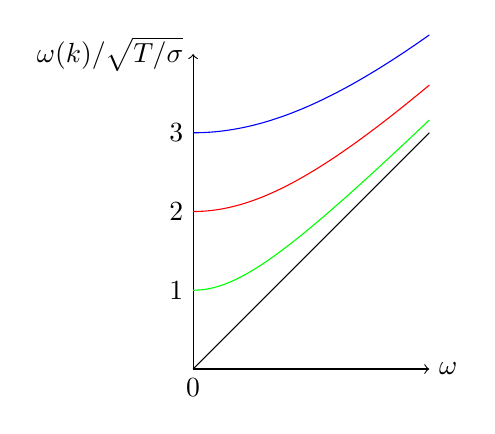
\begin{tikzpicture}
      \draw[->] (0,0) -- (3,0) node[right] {$\omega$};
      \draw[->] (0,0) -- (0,4) node[left] {$\omega(k)/\sqrt{T/\sigma}$};
      \draw[domain=0:3,smooth,variable=\x,black] plot ({\x},{\x});
      \draw[domain=0:3,smooth,variable=\x,green] plot ({\x},{sqrt(\x^2+1)});
      \draw[domain=0:3,smooth,variable=\x,red] plot ({\x},{sqrt(\x^2+2^2)});
      \draw[domain=0:3,smooth,variable=\x,blue] plot ({\x},{sqrt(\x^2+3^2)});
      \draw (0,0) node[below]{0};
        \draw (0,1) node[left]{1};
        \draw (0,2) node[left]{2};
        \draw (0,3) node[left]{3};
\end{tikzpicture}
\end{center}
\item If the membrane resists bending, the wave equation will be a fourth order differential equation, with linear combinations of $k^4$, $q^4$ and $k^2q^2$ in the dispersion relation, hence even the unguided waves will be dispersive, i.e. with phase velocity $\frac{\omega}{k}=O(k^3)$.
\end{enumerate}
\end{ans}
\newpage
\subsubsection{Section C}
\begin{qns}[Structure]
Condensed matter physics has a foundation in understanding the structure of materials.
\begin{enumerate}[label=(\alph*)]
\item Explain the terms Bravais Lattice, unit cell and primitive unit cell.\hfill\textbf{[3]}
\item If iron [atomic mass 56] can be modelled as a solid sphere of radius 0.124 nm, determine: the volume of the primitive unit cell and the density of iron in both the FCC and BCC forms.\hfill\textbf{[6]}
\item Explain the concept of the reciprocal lattice and how it is calculated from the lattice vectors of a material.\hfill\textbf{[3]}
\item A single crystal of iron is heated and undergoes a BCC - FCC phase transition. Describe how the reciprocal lattice of the material will evolve during this process.\hfill\textbf{[3]}
\item Suggest an experimental technique that could be used to probe the structure of iron as it is heated. What problems might occur with making measurements as a result of the BCC - FCC phase transition? How might the new structure be probed?\hfill\textbf{[5]}
\end{enumerate}
\end{qns}
\begin{ans}\leavevmode
\begin{enumerate}[label=(\alph*)]
\item The set of Bravais lattices are those which tessellate to fill the entire 3D space. There are only 14 of them, and can be used to classify crystal structures. At each lattice point is a motif which is replicated in the same orientation at each lattice point. To get from any lattice point to any other point, the displacement vector is $\mathbf{r}=\ell\mathbf{a}+m\mathbf{b}+n\mathbf{c}$, where $\ell,m,n\in\mathbb{Z}$ and $\mathbf{a},\mathbf{b},\mathbf{c}$ are the lattice vectors.\\[5pt]
The primitive unit cell is the smallest repeating unit, and is a parallelepiped spanned by $\mathbf{a}$, $\mathbf{b}$ and $\mathbf{c}$, with a lattice point in each corner and have a volume $\mathbf{a}\cdot(\mathbf{b}\times\mathbf{c})$. A unit cell is allowed to have more than one lattice point in it, and also tessellates to completely fill the space.
\item For both cases, let the conventional cubic unit cell have dimensions $a\times a \times a$. 
\begin{itemize}
    \item For FCC: 4 atomic radii along one face diagonal $4r=\sqrt{2}a$, each cell has $8\times(1/8)+6\times(1/2)=4$ lattice points, the volume of the primitive unit cell is 
    $$V=\frac{1}{4}a^3=\frac{1}{4}(2\sqrt{2}r)^3=4\sqrt{2}r^3=1.08\times10^{-29}m^3$$
    and density $=\frac{56\times1.66\times10^{-27}}{1.68\times10^{-29}}=8620 kgm^{-3}$.
    \item For BCC: 4 atomic radii along one body diagonal $4r=\sqrt{3}a$, each cell has $8\times(1/8)+1=2$ lattice points, the volume of the primitive unit cell is
    $$V=\frac{1}{2}a^3=\frac{1}{2}\bigg(\frac{4r}{\sqrt{3}}\bigg)^3=\frac{32r^3}{3^{3/2}}=1.17\times10^{-29}m^3$$
    and density $=\frac{56\times1.66\times10^{-27}}{1.17\times10^{-29}}=7950 kgm^{-3}$.
\end{itemize}
\item Given a set of lattice vectors $\mathbf{a}$, $\mathbf{b}$ and $\mathbf{c}$, and any arbitrary vector $\mathbf{d}$ is written in terms of this basis:
$$\mathbf{d}=\alpha\mathbf{a}+\beta\mathbf{b}+\gamma\mathbf{c}$$
each of the coefficients is projected out by dotting with the reciprocal lattice vectors
$$\mathbf{A}=\frac{\mathbf{b}\times\mathbf{c}}{[\mathbf{a},\mathbf{b},\mathbf{c}]},\quad\mathbf{B}=\frac{\mathbf{c}\times\mathbf{a}}{[\mathbf{a},\mathbf{b},\mathbf{c}]},\quad\mathbf{C}=\frac{\mathbf{a}\times\mathbf{b}}{[\mathbf{a},\mathbf{b},\mathbf{c}]}$$
i.e. $\alpha=\mathbf{d}\cdot\mathbf{A}=\frac{\alpha\mathbf{a}\cdot(\mathbf{b}\times\mathbf{c})}{[\mathbf{a},\mathbf{b},\mathbf{c}]}$. In materials, we are often concerned with phase shifts from one lattice point to another, so we consider terms like $\mathbf{k}\cdot\mathbf{r}=\frac{2\pi}{\lambda}\mathbf{\hat{k}}\cdot\mathbf{r}$ and so if $\mathbf{k}$ is expressed in terms of the reciprocal lattice, it allows for easier calculation. Reciprocal lattice is also the Fourier transform of the real space lattice, and so describes the Fraunhofer diffraction pattern of crystals.
\item Since FCC and BCC form a Fourier transform pair, the diffraction pattern will switch from that of BCC to that of FCC. Furthermore, Iron expands with heating, so the scale of the diffraction pattern will shrink.
\item Neutron diffraction is useful during the phase transition, where we do not expect to see a uniform periodic crystal structure. The new structure is periodic again and we can use X-ray diffraction. For such temperature induced transition, the temperature has to be increased slowly to achieve uniform transition. This is done by placing all sides of the crystal to be in contact with a thermal bath. To measure at constant pressure, contacts have to be moveable with no friction.
\end{enumerate}
\end{ans}
\newpage
\begin{qns}[Band Structure]
The free and nearly free electron model.
\begin{enumerate}[label=(\alph*)]
\item Outline some of the ‘failures’ of the free electron model and the differences in approach taken in the nearly free electron model.\hfill\textbf{[4]}
\item Given the form of the Bloch function, $\psi(x)=u(x)e^{i\phi x}$, show that for atoms spaced a distance a apart in a 1D loop of $N$ atoms,
$$\phi=\frac{2\pi n}{Na}$$
where $x$ is a variable representing the distance around the loop and $n$ is an integer.\hfill\textbf{[4]}
\item Using Bloch’s Theorem, solve the Schr\"{o}dinger Equation for the potential relating to the loop of atoms in (b),
$$V(x)=\alpha\sum_{j=0}^{N-1}\delta(x-ja)$$
to show that
$$\cos(\phi a)=\frac{m\alpha}{k\hbar^2}\sin(ka)+\cos(ka)$$
where $k^2 = 2mE/\hbar^2$.\hfill\textbf{[8]}
\item Taking $a = 1$ sketch how $\cos(\phi a)$ varies with $k$, for the case where $m\alpha/\hbar^2=10$ and comment on the implications for the electronic properties of the material.\hfill\textbf{[4]}
\end{enumerate}
\begin{mdframed}
\color{darkblue}{The derivative across the delta function satisfies the following:
$$\Delta\psi'(0)=\psi'_+(0)-\psi_-'(0)=\frac{2m\alpha}{\hbar^2}\psi(0)$$
}
\end{mdframed}
\end{qns}
\begin{ans}\leavevmode
\begin{enumerate}[label=(\alph*)]
\item The free electron model asserts that all crystals are metals, and so fails to account for the existence of semiconductors. Also it incorrectly predicts that the Hall coefficient will always be negative. It also fails to account for anisotropy in conductivity (electrical or thermal), and many magnetic effects. 
\item We have periodic boundary conditions, so
$$\psi(x+Na)=\psi(x)\implies u(x+Na)e^{i\phi x}e^{i\phi Na}=u(x)e^{i\phi x}$$
Bloch's theorem requires $u(x)=u(x+a)$ for a lattice with periodicity $a$, leaving us with $e^{i\phi Na}=1\implies\phi=\frac{2\pi n}{Na}$.
\item We wish to solve the Schr\"{o}dinger's equation
$$-\frac{\hbar^2}{2m}\frac{\partial^2\psi}{\partial x^2}+\alpha\sum_{j=0}^{N-1}\delta(x-ja)\psi=E\psi$$
For $x\neq ja$ $\forall j$, $u=A\sin kx+B\cos kx$ with $k=\sqrt{2mE}/\hbar^2$. Going from one cell to the next, we proved above that the wavefunction gains an extra phase of $e^{i\phi a}$, we replace $u(x)$ with $u(x+a)$.
$$\psi(x)=
\left\{
        \begin{array}{ll}
      e^{-i\phi a}(A\sin (k(x+a))+B\cos(k(x+a)) & -a<x<0 \\
      A\sin(kx)+B\cos(kx) & 0<x<a
      \end{array}
    \right.$$
Invoke continuity conditions: $\psi$ continuous at $x=0$
$$e^{-i\phi a}(A\sin ka+B\cos ka)=B$$
$\psi'$ discontinuous at $x=0$
$$kA-e^{-i\phi a}(Ak\cos ka-Bk\sin ka)=\frac{2m\alpha}{\hbar^2}B$$
Matriculate the two equations, and ensure determinant vanish, then we get a desired equation.
\item Sketch $\cos\phi=10\sin k/k+\cos k$.
\end{enumerate}
\begin{center}
\begin{tikzpicture}
      \draw[->] (0,0) -- (15,0) node[right] {$k$};
      \draw[->] (0,-1.5) -- (0,5.5) node[left] {$\cos\phi$};
      \draw[domain=0.1:14,smooth,variable=\x,black] plot ({\x},{4*sin(deg(\x))/(\x)+cos(deg(\x)))});
      \draw (0,0) node[left]{0};
\end{tikzpicture}
\end{center}
\end{ans}
\subsubsection{Section D}
\begin{qns}[OWO Essay]
Write an essay describing wave propagation in various media.

\hfill\textbf{[20]}
\end{qns}
\begin{ans}
There are two types of travelling waves. We have 
\begin{itemize}
    \item transverse wave:
    displacement of the medium is perpendicular to the direction of wave propagation
    \item longitudinal wave: displacement of the medium is in the same direction as the direction of wave propagation
\end{itemize}
A common example of transverse wave is the electromagnetic wave which can travel in any media including vacuum. Of course, this will be a travelling wave as long as the wavenumber $k$ in the medium is still real and not imaginary. Otherwise, the wave would be an exponentially decaying evanescent wave that is not propagating through the medium.\\[5pt]
For longitudinal wave, it requires a medium to propagate through. Let's first consider a 1D tube of air inside a cylindrical container with cross-sectional area $A$. Let the ends of this section be located at $x$ and $x+\Delta x$ at equilibrium, and then at $x+\psi(x)$ and $x+\Delta x+\psi(x+\Delta x)$ at a later time. The function $\psi$ measures the longitudinal displacement from equilibrium. If we define $\Delta\psi$ to be $\psi(x+\Delta x)=\psi(x)+\Delta\psi$, where $\Delta\psi$ is how much more the right boundary of the region moves compared with the left boundary.\\[5pt]
Let the pressure in the tube at equilibrium be $p_0$. Let $\psi_p(x)$ be the excess pressure above $p_0$ as a function of $x$. The total pressure at the left boundary and the right boundary are $\psi_p(x)$ and $\psi_p(x+\Delta x)=\psi_p(x)+\Delta\psi_p$, where $\Delta\psi_p$ is how much the pressure at the right boundary exceeds the pressure at the left boundary.\\[5pt]
The change in volume from equilibrium $\Delta V=A\Delta\psi$ is directly proportional to $-V\psi_p$, where $\Delta V/V<<1$. Let the compressibility $\kappa$ be the desired constant of proportionality, then $$\frac{\partial\psi}{\partial x}=-\kappa\psi_p\implies\frac{\partial\psi_p}{\partial x}=-\frac{1}{\kappa}\frac{\partial^2\psi}{\partial x^2}$$
For ideal gas, we have isothermal compressibility be $\kappa=\frac{1}{p_0}$ and for adiabatic compressibility be $\kappa=\frac{1}{\gamma p_0}$. We will use the latter. The net force is $F_{net}=A(p(x)-p(x+\Delta x))=A(p_0+\psi_p(x)-p_0-\psi_p(x+\Delta x))=A(-\Delta\psi_p)$ and so
$$\rho A\Delta x\frac{\partial^2\psi}{\partial t^2}=-A\bigg(-\frac{1}{\kappa}\frac{\partial^2\psi}{\partial x^2}\Delta x\bigg)\implies\frac{\partial^2\psi}{\partial t^2}=\frac{\gamma p_0}{\rho}\frac{\partial^2\psi}{\partial x^2}$$
The longitudinal displacement does satisfy the wave equation. Taking $\frac{\partial}{\partial x}$ yields $$\frac{\partial^2}{\partial t^2}\frac{\partial\psi}{\partial x}=\frac{\gamma p_0}{\rho}\frac{\partial^2}{\partial x^2}\frac{\partial\psi}{\partial x}$$
Since $\frac{\partial\psi}{\partial x}$ is directly proportional to $\psi_p$, we have the desired wave equation for excess pressure. The wave speed is  $c=1/\sqrt{\rho/\gamma p_0}=1/\sqrt{\kappa\rho}$. The pressure leads the displacement by a phase $\pi/2$ and has amplitude $\frac{k}{\kappa}\psi$. For a harmonic wave of the form $\psi(x,t)\propto e^{i(\omega t-kx)}$, then $\psi_p(x,t)=-\frac{1}{\kappa}\frac{\partial\psi(x,t)}{\partial x}=-\frac{-ik}{\kappa}\psi(x,t)$. The excess force that a sheet of gas exerts on the region to its right is $$F=A\psi_p=A\bigg(-\frac{1}{\kappa}\frac{\partial\psi}{\partial x}\bigg)=-\frac{A}{\kappa}\bigg(\mp\frac{1}{c}\frac{\partial\psi}{\partial t}\bigg)=\frac{\pm A}{\kappa c}\frac{\partial\psi}{\partial t}$$
where we used the harmonic wave form. Hence, the acoustic impedance  $Z_{acous}$ (impedance per cross-sectional area) of the gas is $$Z_{acous}=\frac{1}{A}\frac{F}{\partial\psi/\partial t}=\frac{1}{\kappa c}=\sqrt{\rho/\kappa}=\sqrt{\gamma p_0\rho}$$
The energy density per unit volume can be shown to be $\rho(\frac{\partial\psi}{\partial t})^2$ where $A\rho=\mu$. The power on the sheet of particles whose equilibrium position is $x$ is $P=(p_0+\psi_p)A\frac{\partial\psi}{\partial t}$. Since $\psi_p=-\frac{1}{\kappa}\frac{\partial\psi}{\partial x}$, then $$P=\pm\frac{A}{\kappa c}\bigg(\frac{\partial\psi}{\partial t}\bigg)^2=\pm\frac{Ac^2\kappa^2}{\kappa c}\psi_p=\frac{c}{\rho c^2}\psi_p=\frac{\psi_p}{\rho c}$$ 
Alternatively, using the acoustic impedance $Z_{acous}=\rho c$, we have $P=\pm Z_{acous}(\frac{\partial\psi}{\partial t})^2$. The mean power per unit area, or intensity, is  $\frac{1}{2}Z_{acous}\omega^2|\psi_0|^2$. We can express the intensity of sound as a power level in decibels:
$$10\log_{10}(I/I_{ref})$$
with $I_{ref}=p_{ref}^2/Z_{acous}$ which is $10^{-12}$ W/m$^2$, where $Z_{acous}$ for air is 400 kg m$^{-2}$ s$^{-1}$.\\[5pt]
Extending these ideas to solids and liquids: We have the general relation $$\psi_p=-\kappa\frac{\partial\psi}{\partial x}$$
$\kappa$ could be the bulk modulus of a liquid or Young's modulus of a solid (which is ratio of stress to strain).
\end{ans}
\newpage
\begin{qns}[CMP Short Notes]
Write brief notes on two of the following:\hfill\textbf{[20]}
\begin{itemize}
    \item the Hall effect;
    \item doping in semiconductors;
    \item thermal conductivity of metals.
\end{itemize}
\end{qns}
\begin{ans}\leavevmode
\subsubsection*{The Hall Effect:}
An electrical field $E_x$ is applied to a wire extending in the $x$-direction and a current density $J_x$ flows in the wire. In addition, the magnetic field $\mathbf{B}$ points in the positive $z$-direction, resulting in a Lorentz force $-e\mathbf{v}\times\mathbf{B}$ which  acts to deflect electrons in the negative $y$-direction. However, the electrons cannot move very far in the $y$-direction before running up against the sides of the wire. As they accumulate there, an electric field builds up in the $y$-direction that opposes their motion and their further accumulation.\\[5pt]
In equilibrium, this transverse field (Hall field) $E_y$ will balance the Lorentz force and current will flow only in the $x$ direction. The magnetoresistance is $\frac{E_x}{J_x}$, which Hall found to be field-independent. Moreover, since the transverse field $E_y$ balances the Lorentz force, one might expect it to be proportional both to the applied field $H$ and to the current along the wire $J_x$, hence the Hall coefficient is $R_H=\frac{E_y}{J_xB}$.
$$\frac{d}{dt}\mathbf{p}=-e\bigg(\mathbf{E}+\frac{\mathbf{p}}{m}\times\mathbf{B}\bigg)-\frac{\mathbf{p}}{\tau}$$
In the steady state the current is independent of time, i.e. $\frac{d}{dt}\mathbf{p}$ and so we get $\omega_c=\frac{eB}{m}$. We have
$$\sigma_0E_x=\omega_c\tau J_y+J_x,\quad \sigma_0E_y=-\omega_c\tau J_x+J_y$$
where $\sigma_0=ne^2\tau/m$ is the Drude model DC conductivity in the absence of a magnetic field. The Hall field $E_y$ is determined by the requirement that there be no transverse current $J_y$, i.e. $J_y=0\implies E_y=-\frac{B}{ne}J_x$ so the Hall coefficient is $R_H=-\frac{1}{ne}$. The Hall coefficient measurement of the density seems reasonable for many metals. But yet, the Hall coefficient is frequently measured to have the wrong sign, indicating a charge carrier with charge opposite to that of the electron.
\subsubsection*{Doping in Semiconductors:}
Adding dopants that gives more (fewer) electrons than the substrate itself creates an n-type (a p-type) semiconductor. At non-zero temperatures, all these states are ionized, increasing the conductance of the material. For the n-type (p-type), the vast majority of the charge carriers are ionized electrons (holes left behind when electrons from the filled band were excited into the dopant hole state). In the absence of impurities, the Fermi energy ($\mu(T=0)$) is in the middle of the band gap. When the donor (acceptor) impurities are added, at zero temperature, impurity states near the top (bottom) of the bandgap are filled (empty). The Fermi energy is moved up to the top (down to the bottom) of the band gap.\\[5pt]
Although the n-doped system has free negatively charged electrons and the p-doped system has free positively charged holes, both systems are overall electrically neutral since charged ions compensate for the charges of the mobile charge carriers. When the two doped semiconductors are brought into contact, the electrons in the conduction band will fall into the valence band, filling the empty hole states, thus pair-annihilating both the electron and the hole. This amounts to a gain in energy of $E_{gap}$ per pair annihilated.\\[5pt]
After this process of electrons falling into holes and annihilating occurs there will be a region near the interface where there are no free carriers at all. This is the depletion region, which is electrically charged (since there are charged ions but no carriers to neutralize them). Hence, there is a net electric field pointing from the positively charged to the negatively charged ions.
\newpage
\subsubsection*{Thermal conductivity of metals:}
In the free electron model (FEM), each lattice point contributes $n$ delocalized electrons ($n$ is valency). The rest are regarded as core electrons and together with the nuclei, they form a uniform background potential. With this in mind, we can predict the transport properties of these solids using the classical Drude model. The assumptions of Drude model are
\begin{enumerate}
    \item Independent electron approximation: neglect electron-electron interactions between collisions; Free electron approximation: neglect electron-ion interactions. The electrons respond solely to the externally applied fields.
    \item Collisions are instantaneous events that abruptly alter the velocity of an electron. Drude attributed them to the electrons bouncing off the impenetrable ion cores.
    \item Electron experiences a collision with a probability per unit time $1/\tau$, where $\tau$ is the relaxation time. An electron picked at random at a given moment will, on the average, have been travelling for a time $\tau$ before its next collision, and will, on the average, have been travelling for a time $\tau$ since its last collision. $\tau$ is independent of the electron's position and velocity.
    \item Electrons are assumed to achieve thermal equilibrium with their surroundings only through collisions. Immediately after each collision, an electron is taken to emerge with a velocity that is not related to its velocity just before the collision, but randomly oriented and with a speed appropriate to the temperature prevailing at the place where the collision occurred.
\end{enumerate}
The most impressive success of the Drude model was to account for the empirical law of Wiedemann and Franz. The law states that the ratio of thermal conductivity $\kappa$ to electrical conductivity $\sigma$ is directly proportional to the temperature. Here, we assumed the bulk of the thermal current in a metal is carried by the conduction electrons. Consider a metal bar along which the temperatures varies slowly, and no sources and sinks are present. We define the thermal current density $\mathbf{J_q}:=-\kappa\boldsymbol{\nabla}T$.\\[5pt]
Consider first a one-dimensional model. If $\epsilon(T)$ is the thermal energy per electron in a metal in equilibrium at temperature $T$, then an electron whose last collision was at $x'$ will, on the average, have a thermal energy $\epsilon(T[x'])$. The electrons arriving at $x$ from the high-temperature side will, on the average, have had their last collision at $x-v\tau$, and will therefore carry a thermal energy per electron of size $\epsilon(T[x-v\tau])$. Their contribution to the thermal current density at $x$ will therefore be $\frac{n}{2}v\epsilon(T[x-v\tau])$. The electrons arriving at $x$ from the low temperature side will be $-v\frac{n}{2}\epsilon(T[x+v\tau])$. Then we have 
$$J_q\approx nv^2\tau\frac{d\epsilon}{dT}\bigg(-\frac{dT}{dx}\bigg)$$
Extending to three dimensions, we replace $v^2$ with $\frac{1}{3}v^2$ to average over all directions. So,
$$\mathbf{J_q}=\frac{1}{3}v^2\tau c_V(-\boldsymbol{\nabla}T)\implies\kappa=\frac{1}{3}v^2\tau c_V$$
where $c_V$ is the electronic specific heat.\\[5pt]
The ratio is thus $\frac{\kappa}{\sigma}=\frac{c_Vmv^2}{3ne^2}$. Drude further took $c_V=\frac{3}{2}nk_B$ and $\frac{1}{2}mv^2=\frac{3}{2}k_BT$. The ratio becomes
$$\frac{\kappa}{\sigma T}=\frac{3k_B^2}{2e^2}$$
which is the Lorenz number. Drude theory is successful in accounting for the value of Wiedemann-Franz ratio. 
\end{ans}
\end{document}